\documentclass[UKenglish]{uiomasterthesis} %% ... or norsk or nynorsk or USenglish
\usepackage[utf8]{inputenc} %% ... or latin1
\usepackage[T1]{url}\urlstyle{sf}
\usepackage{babel, csquotes, graphicx, textcomp, uiomasterfp, varioref}
\usepackage{amsthm}
\usepackage{pgf}
\usepackage{tikz}
\usepackage{amsmath, amssymb, amsfonts, bm}
\usepackage{acronym}
\usepackage{mathtools}
\usepackage{algorithm}
\usepackage{listings}
\usepackage[table]{xcolor}
\usepackage{listofitems}
\usepackage{algpseudocode}
\usepackage{tikzlings}
\usepackage[backend=biber,style=numeric-comp, sorting=none]{biblatex}
\usepackage[hidelinks, hypertexnames=false]{hyperref}


\usetikzlibrary{arrows.meta} % for arrow size
\usepackage[outline]{contour} % glow around text
\contourlength{1.4pt}

\usetikzlibrary{positioning, matrix, backgrounds}
\usetikzlibrary{3d,decorations.text,shapes.arrows,fit}

\definecolor{codegreen}{rgb}{0,0.6,0}
\definecolor{codegray}{rgb}{0.5,0.5,0.5}
\definecolor{codepurple}{rgb}{0.58,0,0.82}
\definecolor{backcolour}{rgb}{0.95,0.95,0.92}

\lstdefinestyle{pythonstyle}{
    language=Python,
    backgroundcolor=\color{white},
    commentstyle=\color{codegreen},
    keywordstyle=\color{magenta},
    numberstyle=\tiny\color{codegray},
    stringstyle=\color{codepurple},
    basicstyle=\ttfamily\footnotesize,
    breakatwhitespace=false,
    escapeinside=||,
    breaklines=true,
    captionpos=b,
    keepspaces=true,
    frame=single,
    numbersep=5pt,
    showspaces=false,
    showstringspaces=false,
    showtabs=false,
    tabsize=2,
    morekeywords={self},
}

\lstset{
	breaklines=true,
	style=pythonstyle,
}


\let\origthelstnumber\thelstnumber
\makeatletter
\newcommand*\Suppressnumber{%
  \lst@AddToHook{OnNewLine}{%
    \let\thelstnumber\relax%
     \advance\c@lstnumber-\@ne\relax%
    }%
}

\newcommand*\Reactivatenumber[1]{%
  \setcounter{lstnumber}{\numexpr#1-1\relax}
  \lst@AddToHook{OnNewLine}{%
   \let\thelstnumber\origthelstnumber%
   \refstepcounter{lstnumber}
  }%
}


\makeatother


\tikzset{pics/fake box/.style args={% #1=color, #2=x dimension, #3=y dimension, #4=z dimension
#1 with dimensions #2 and #3 and #4 and #5}{
code={
\draw[thin]  (0,0,0) coordinate(-front-bottom-left) to
++ (0,#3,0) coordinate(-front-top-right) --++
(#2,0,0) coordinate(-front-top-right) --++ (0,-#3,0) 
coordinate(-front-bottom-right) -- cycle;
\draw[thin] (0,#3,0)  --++ 
 (0,0,#4) coordinate(-back-top-left) --++ (#2,0,0) 
 coordinate(-back-top-right) --++ (0,0,-#4)  -- cycle;
\draw[thin] (#2,0,0) --++ (0,0,#4) coordinate(-back-bottom-right)
--++ (0,#3,0) --++ (0,0,-#4) -- cycle;
\path[decorate,decoration={text effects along path, text={#5}}] (#2/2,{2+(#3-2)/2},0) -- (#2/2,0,0);
}
}}
% from https://tex.stackexchange.com/a/52856/121799
\tikzset{circle dotted/.style={dash pattern=on .05mm off 2mm,
                                         line cap=round}}

\pgfdeclarelayer{foreground}
\pgfsetlayers{background, main, foreground}

\renewcommand{\algorithmicrequire}{\textbf{Input:}}
\renewcommand{\algorithmicensure}{\textbf{Output:}}
\newcommand{\R}{\mathbb{R}}

\providecommand{\mathdefault}[1]{#1}


\definecolor{id}{rgb}{0.4, 0.7607843137254902, 0.6470588235294118}
\definecolor{near}{rgb}{0.5529411764705883, 0.6274509803921569, 0.796078431372549}
\definecolor{far}{rgb}{0.9882352941176471, 0.5529411764705883, 0.3843137254901961}

\definecolor{ca0a0a0}{RGB}{160,160,160}
\definecolor{ce0e0e0}{RGB}{224,224,224}
\colorlet{myred}{red!80!black}
\colorlet{myblue}{blue!80!black}
\colorlet{mygreen}{green!60!black}
\colorlet{myorange}{orange!70!red!60!black}
\colorlet{mydarkred}{red!30!black}
\colorlet{mydarkblue}{blue!40!black}
\colorlet{mydarkgreen}{green!30!black}

% STYLES
\tikzset{
  >=latex, % for default LaTeX arrow head
  node/.style={thick,circle,draw=myblue,minimum size=22,inner sep=0.5,outer sep=0.6},
  node in/.style={node,green!20!black,draw=mygreen!30!black,fill=mygreen!25},
  node hidden/.style={node,blue!20!black,draw=myblue!30!black,fill=myblue!20},
  node convol/.style={node,orange!20!black,draw=myorange!30!black,fill=myorange!20},
  node out/.style={node,red!20!black,draw=myred!30!black,fill=myred!20},
  connect/.style={thick,mydarkblue}, %,line cap=round
  connect arrow/.style={-{Latex[length=4,width=3.5]},thick,mydarkblue,shorten <=0.5,shorten >=1},
  node 1/.style={node in}, % node styles, numbered for easy mapping with \nstyle
  node 2/.style={node hidden},
  node 3/.style={node out}
}
\def\nstyle{int(\lay<\Nnodlen?min(2,\lay):3)} % map layer number onto 1, 2, or 3

\title{Explainable Artificial Intelligence for Out-of-Distribution Detection}
\subtitle{Using irregularities in machine learning explanations to detect when a model is faced with unusual data}
\author{Jonatan Hoffmann Hanssen}

\addbibresource{bibliography.bib}

\theoremstyle{definition}
\newtheorem*{definition}{Definition}

\begin{document}


\uiomasterfp[dept={Department of Informatics},
program={Robotics and Intelligent Systems},
supervisors={Hugo Lewi Hammer \and Kyrre Harald Glette}, image={/home/jona/.config/zsh/cat.jpg},
long]

\frontmatter{}
\begin{abstract}
As Artificial Intelligence becomes a larger and larger part of society, the need for robust and understandable models becomes paramount. When neural networks are used in high-impact settings such as cancer detection or autonomous driving, we must require that they 
\end{abstract}

\begin{xabstract}[Sammendrag]
Here comes the abstract in a different language.
\end{xabstract}

\tableofcontents{}
\listoffigures{}
\listoftables{}

\begin{acronym}[ICANN]
    \acro  {ood}   [OOD]   {Out-of-Distribution}
    \acro  {dl}   [DL]   {Deep Learning}
    \acro  {id} [ID] {In-Distribution}
    \acro  {cam} [CAM] {Class Activation Mapping}
    \acro  {gradcam} [GradCAM] {Gradient Class Activation Mapping}
    \acro  {gap}   [GAP]   {Global Average Pooling}
    \acro  {msp}   [MSP]   {Maximum Softmax Probability}
    \acro  {lime}   [LIME]   {Local Interpretable Model-Agnostic Explanations}

    \acro  {cnn}   [CNN]   {Convolutional Neural Network}

    \acro  {slic} [SLIC] {Simple Linear Iterative Clustering}

    \acro  {ffnn}[FFNN]{Feed Forward Neural Network}

    \acro  {ml}   [ML]   {Machine Learning}
    \acro  {lrp}   [LRP]   {Layer Relevance Propagation}
    \acro  {xai}   [XAI]   {Explainable Artificial Intelligence}
    \acro  {ai}   [AI]   {Artificial Intelligence}
    \acro  {auroc}   [AUROC]   {Area Under Receiver Operating Characteristic}
    \acro  {aupr}   [AUPR]   {Area Under Precision Recall Curve}
    \acro  {roc}   [ROC]   {Receiver Operating Characteristic}
    \acro  {fpr}   [FPR]   {False Positive Rate}
    \acro  {tpr}   [TPR]   {True Positive Rate}
    \acro  {fpr95}   [FPR95]   {False Positive Rate at 95\% Recall}
\end{acronym}

\begin{preface}
I would like to thank my dog and Ed Bickley, who is still at large.
\end{preface}

\mainmatter{}



\chapter{Introduction}

\section{Motivation}

\ac{ml} generally, and \ac{dl} specifically, have seen a tremendous increase in performance in recent years, performing comparable to humans in tasks such as image classification, speech and handwriting recognition, as well as many others \cite{performance}. Consequently, \ac{dl} methods have been deployed in a multitude of fields and have become a part of our daily lives through their role in web search, text translation, computer vision, and in many other technologies which are taken for granted. In medicine, deep learning has the potential to provide faster and more accurate detection of diseases by being trained on cases from thousands of previous patients \cite{xaisurvey}. Despite this, "surprisingly little in health care is driven by machine learning" \cite{dlmed}.

% TODO: make these citations more specific

To explain this discrepancy, we should consider that despite their impressive performance, the application of deep learning methods is not without drawbacks. Firstly, deep neural networks are inherently unexplainable due to the large number of parameters that any non-trivial network has. State of the art models will perform millions of operations to evaluate a single data point, and it is therefore impossible for humans to comprehend and explain the entire process which lead the model to make a particular decision. In medicine, this is a major limitation of deep learning methods, as both doctors and patients expect to be able to understand why a decision was made \cite{tingsim}.

Secondly, although neural networks may attain high accuracy on test data and appear to have learned great insights about the tasks they are employed in, they often lack robustness and can suffer large drops in performance on data points which are slightly different from the training data. As \cite{intriguing} has shown, it is possible to create data points which are imperceptibly different from normal data points, yet still fool otherwise high performing models. More problematically, unlike humans, who recognize when they are faced with a novel situation where their expertise might be lacking, \ac{dl} methods will predict equally confidently on data points which are far outside the data they have been trained on \cite{tingsim}.

These two problems lead to the fields of \ac{xai}, and \ac{ood} detection. \ac{xai} attempts to explain the reasons why a model came to a decision, which helps to remedy the black-box nature of complicated \ac{dl} models. In a healthcare setting, such explanations can be inspected by medical practitioners to confirm the diagnosis, and can be used to give patients information about why decisions regarding their health were made. \ac{ood} detection attempts to uncover when a data point is too different from the training data to be classified reliably. These methods could alert medical practitioners when such data points occur, thus avoiding potentially fatal misclassifications.

Both of these fields have seen increased interest in recent years, and are vital parts of any integration of \ac{dl} in medical settings. This thesis will focus on \ac{ood} detection, but will attempt to use methods inspired by \ac{xai} to improve detection performance. The overarching intuition is that by inspecting the explanation of a model on a specific data point, we may be able to uncover flaws or irregularities in the explanation which could help us determine whether the data point is \ac{ood}.

% This thesis will attempt to combine the two fields, by using methods inspired by \ac{xai} to improve \ac{ood} detection.

\section{Problem Statement} \label{section:problemstatement}

As explained in the previous segment, \ac{ood} detection is a developing field, which has become more important in recent years as machine learning is being used for higher impact tasks, such as disease detection. Finding novel methods which improve a model's ability to detect when input is \ac{ood} is important to increase the robustness of machine learning models as they are used in these real-world scenarios. The field of \ac{xai} is concerned with understanding the inner workings of a model, and could thus offer insights which could help us detect unusual behaviour in the model as a result of \ac{ood} data points. The problem statement is thus as follows:

\textbf{Can methods from the field of Explainable Artificial Intelligence be used to improve Out-of-Distribution Detection?}
\\

To answer this question, I introduce 2 objectives:

\begin{enumerate}
  % \item Perform comprehensive analysis of the properties of explanations generated by a number of \ac{xai} algorithms on ID and \ac{ood} samples, highlighting differences that could aid \ac{ood} detection.
    \item Develop \ac{ood} detection methods which rely solely on \ac{xai} explanations, and compare these methods 
    \item Develop theoretically sound proof of concept \ac{ood} detection methods that are inspired by insights gained from the field of \ac{xai}, and compare these methods on a variety of different benchmarks against existing \ac{ood} detection methods
\end{enumerate}

\section{Scope} \label{section:scope}

As we will see in chapter \ref{chapter:background}, both the fields of \ac{xai} and \ac{ood} detection are very large, which make it impossible to explore all the possible ways one might combine \ac{xai} and \ac{ood} detection. Thus, it is necessary to restrict the scope of both the \ac{xai} and \ac{ood} detection methods used. In this section, I will describe the choices I've made and give a short explanation. In later chapters, the choices will be justified more thoroughly.

The field of \ac{ood} detection is primarily concerned with image classification tasks. Thus, my project will also deal exclusively with image classification datasets. Given this type of data, the choice of \ac{xai} algorithms naturally gravitates towards post-hoc, saliency based methods. The choice of \ac{ood} detection algorithms is not significantly restricted by the choice to deal exclusively with image data, but I will exclude methods which use outlier exposure to improve performance, or which require retraining of the model. These choices are informed by \cite{openood}, which have found that post-hoc methods

% Use only post-hoc methods, pretrained resnet models. Use well established \ac{ood} datasets first for comparisons. Then focus on medical datasets, hyperkvasir and maybe more. Only use open-source programs. Python and Pytorch. Mainly focus on images. Probably only \ac{cnn} models, as a lot of \ac{xai} is based on that. Maybe also try methods that work on vision transformers as well, but then we are more restricted to post-hoc methods probably.

\section{Research Methods}

Use ACM

\section{Ethical Considerations}


\section{Main Contributions}

Objective 1 is accomplished in chapter \ref{chapter:background}. Here, the fields of \ac{xai} and \ac{ood} detection are introduced, their respective taxonomies are explained and a selection of specific methods are explained in more detail. This chapter provides a good entry for machine learning researchers who wish a decent introduction to the two fields.

\section{Thesis Outline}

Chapter \ref{chapter:background} gives a short introduction to machine learning, followed by a deeper look at the fields of \ac{xai} and \ac{ood} detection. Chapter \ref{chapter:methodology} introduces my methodology; the methods I will use to compare and contrast \ac{xai} explanations on ID and \ac{ood} data, as well as a handful of \ac{ood} detection methods which integrate explanations into their functioning. Furthermore, I introduce the different datasets which will be used in chapter \ref{chapter:experiments}, among them the HyperKvasir gastrointestinal dataset \cite{hyperkvasir}. \ref{chapter:experiments} will first go into the results of the comparison between ID and \ac{ood} explanations, detailing the differences between different methods. Then, I will report the performance of the different \ac{ood} detection algorithms I have developed, on a handful of datasets, including HyperKvasir, CIFAR10 and ImageNet. After the experiments follow a discussion (chapter \ref{chapter:discussion}), where I reflect on the benefits and drawbacks of using \ac{xai} methods for \ac{ood} detection, and summarize the results from \ref{chapter:experiments}. Finally, the conclusion (chapter \ref{chapter:conclusion}) concludes.

\chapter{Background} \label{chapter:background}

In this chapter I give a short introduction to important concepts in the field of machine learning generally, followed by a more in-depth look at the fields of \ac{ood} detection and \ac{xai}. Then, I give an overview of related works; papers which have attempted to use \ac{xai} for \ac{ood} detection. Finally, the datasets used in chapter \ref{chapter:experiments} are covered. 

\section{Machine Learning}

Machine Learning is the field of algorithms that are able to learn from data, as opposed to being explicitly programmed. Such algorithms use statistical methods to learn relationships in data, and use these relationships to generalize to unseen data. More formally, \cite{mitchell} gives the following definition of machine learning algorithms:

\begin{definition}
A computer program is said to learn from experience $E$ with respect to some class of tasks $T$ and performance measure $P$ if its performance at tasks in $T$, as measured by $P$, improves with experience $E$.
\end{definition}

Thus, machine learning is a different paradigm from traditional problem solving, where programs are made to solve problems by following explicit rules. For example, a traditional image classification system attempting to differentiate between malignant and benign tumors might use hand-crafted rules which consider the texture, color and size of a tumor. As one might imagine, such rules will quickly become very complicated when we consider all the possible factors which might influence the appearance of a tumor. Using a machine learning approach, we would instead feed an algorithm with thousands of images of both benign and malignant tumors, and the rules could then be automatically updated until the algorithm predicted the correct category with a high enough accuracy.

Machine Learning is commonly divided into the three subcategories of supervised, unsupervised and reinforcement learning

% A simple comparison is between the two chess engines Stockfish and AlphaZero. Stockfish plays chess by evaluating possible moves according to metrics created by humans\footnote{This is actually no longer the case, as the classical evaluation has been replaced by a neural network (a machine learning approach), however, I will pretend that it still is for the sake of argument}, such as valuing a Queen as equivalent to nine pawns and a 

\subsection{Supervised Learning}

Supervised Learning is a subcategory of machine learning where we have a dataset containing both inputs and desired outputs. In the example above, we could use supervised learning by creating a dataset of images of tumors (the input) and corresponding labels which indicate whether each tumor is malignant or benign (the desired output). The learning goal of the algorithm is then to associate images with the correct label. Because we know the correct answer, we are able to fine-tune the algorithm automatically whenever it makes a mistake. However, supervised learning requires labeled data, which can be very costly, especially in the medical domain, where deciding whether a tumor is malignant or benign requires expert knowledge.

\subsection{Unsupervised Learning}

In unsupervised learning, we do not have any labels. In these cases, we might not know whether data points belong to different classes or not. Instead, we can use machine learning to uncover patterns in the data, for example by attempting to cluster the data into different groups and seeing if these groups are sufficiently separated. An example use case could be for fraud detection in a bank. By feeding financial transaction from many different users into an unsupervised learning model and asking it to perform clustering of the data, it might be possible to find a group of users whose transactions differ substantially from the rest, which might indicate that their transactions are fraudulent.

\subsection{Reinforcement Learning}

Reinforcement Learning deals with problems where we do not know exactly what the correct solution is, but we are able to assess whether a given solution is good or not. For example, when controlling a robot arm, it is difficult to say exactly what angles each joint should be for every millisecond when picking up an object, but if the arm does not pick up the object, we know the algorithm has failed. In these problems, the algorithm is trained through reinforcement, where good attempts are rewarded and bad attempts punished.

\section{Neural Networks}

Neural Networks are a class of machine learning algorithms, which have become the clear state of the art in almost all fields where machine learning is applied. Notable examples are computer vision, image classification, speech recognition, text and image generation and machine translation. Neural networks are loosely inspired by our own brains, where neurons are connected together and send information between each other. By connecting thousands of neurons together, neural networks are able to learn complicated relationships between the input and output.

\subsection{Feed Forward Neural Networks}

The \ac{ffnn}, also known as a Multilayer Perceptron, traces its roots to the very beginning of machine learning, through the work of Frank Rosenblatt \cite{rosenblatt}. It forms the basic structure for neural networks which has been adapted and modified over the years to form more complex architectures such as convolutional, recurrent or residual neural networks. The basic structure of an \ac{ffnn} is that the input values are passed through an affine transformation (a matrix multiplication followed by the addition of a bias), and then passed through an activation function, which produces outputs. These outputs can then go through the same process again, which constitutes a single "layer". By stacking several of these layers, with non-linear activation functions, an \ac{ffnn} is able to learn arbitrarily complex mappings between inputs and outputs\footnote{In fact, by the Universal Approximation Theorem \cite{uat}, only a single hidden layer between the input and output is necessary, although this theorem does not give a way to construct such a network for any given function}. Figure \ref{fig:ffnn}\footnote{Figure by Izaak Neutelings, "Neural Network with coefficients, arrows", TikZ.net, licensed under CC BY-SA 4.0, [\url{https://tikz.net/neural\_networks/}].} shows a simple \ac{ffnn} architecture with three hidden layers. In this case, the bias has been omitted for brevity. Here, we can see how all nodes of a layer are connected to the following layer. By using an activation function on the nodes of the hidden layer, before their values are sent to the next layer, we achieve the non-linearity required to learn complex patterns.

\begin{figure}[H]
    \begin{center}

    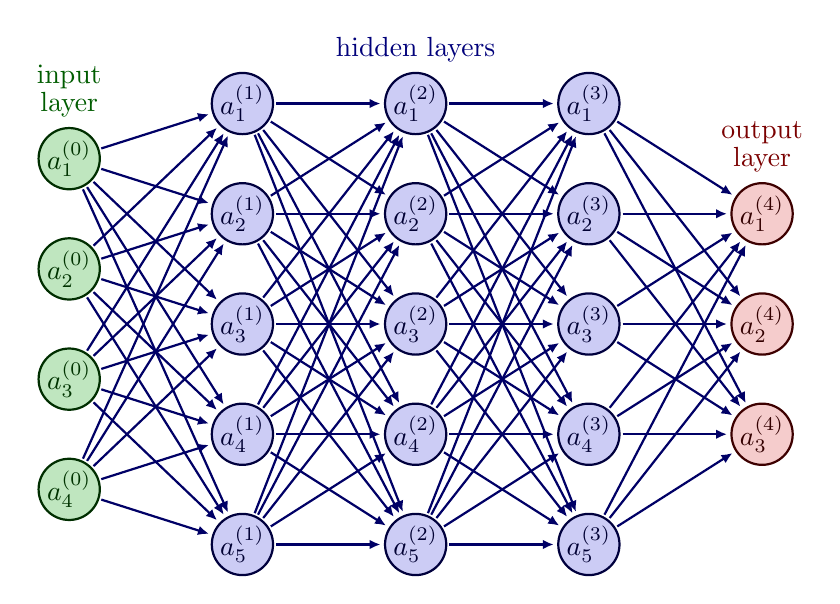
\begin{tikzpicture}[x=2.2cm,y=1.4cm]
  \message{^^JNeural network with arrows}
  \readlist\Nnod{4,5,5,5,3} % array of number of nodes per layer
  
  \message{^^J  Layer}
  \foreachitem \N \in \Nnod{ % loop over layers
    \edef\lay{\Ncnt} % alias of index of current layer
    \message{\lay,}
    \pgfmathsetmacro\prev{int(\Ncnt-1)} % number of previous layer
    \foreach \i [evaluate={\y=\N/2-\i; \x=\lay; \n=\nstyle;}] in {1,...,\N}{ % loop over nodes
      
      % NODES
      \node[node \n] (N\lay-\i) at (\x,\y) {$a_\i^{(\prev)}$};
      %\node[circle,inner sep=2] (N\lay-\i') at (\x-0.15,\y) {}; % shifted node
      %\draw[node] (N\lay-\i) circle (\R);
      
      % CONNECTIONS
      \ifnum\lay>1 % connect to previous layer
        \foreach \j in {1,...,\Nnod[\prev]}{ % loop over nodes in previous layer
          \draw[connect arrow] (N\prev-\j) -- (N\lay-\i); % connect arrows directly
          %\draw[connect arrow] (N\prev-\j) -- (N\lay-\i'); % connect arrows to shifted node
        }
      \fi % else: nothing to connect first layer
      
    }
    
  }
  
  % LABELS
  \node[above=0,align=center,mygreen!60!black] at (N1-1.90) {input\\[-0.2em]layer};
  \node[above=0,align=center,myblue!60!black] at (N3-1.90) {hidden layers};
  \node[above=0,align=center,myred!60!black] at (N\Nnodlen-1.90) {output\\[-0.2em]layer};
  

    \end{tikzpicture}
    \end{center}
    \caption[Feed Forward Neural Network]{Figure showing a simple Feed Forward Neural Network, with nodes labeled. The number in parentheses indicates the layer number while the subscript indicates the node number within the layer.}
    \label{fig:ffnn}
\end{figure}



Mathematically, a single layer can then be described as follows:

\begin{equation}
\bm{x_{i+1}} = \sigma_i (A_i \bm{x_i} + \bm{b_i})
\label{ffnn}
\end{equation}

Here, the input $\bm{x_i}$ is linearly transformed by the weights of the matrix $A_i$ from the input space to the output space, then each value of the new vector in the output space is adjusted by an addition of a bias term, and finally an activation function ($\sigma_i$) is applied to each value. The size of the input and output layers is determined by the number of input and output features, respectively. Furthermore, the activation function of the output layer is also determined by the application, most commonly {\it sigmoid} for binary classification, {\it softmax} for multi-class classification and simply identity for regression.


\subsection{Convolutional Neural Networks}

\acp{ffnn} have some inherent flaws which make them unsuitable for working with high dimensional, spatially connected data, such as the pixels which make up an image. Firstly, each input of a \ac{ffnn} is connected to every output of the following layer. If we want to connect the input pixels of a $224$ by $224$ image to a layer of 100 nodes, our first layer will have over 5 million weights, which is already quite a lot for a relatively small image. Furthermore, these weights will have to encode redundant information, because each pixel is considered separately. Consider a network attempting to detect the presence of a cat in an image. We would want the network to detect the cat regardless of whether it is in the middle, the right corner, or any other position in the image. In an \ac{ffnn}, the weights connected to any of these positions in the image would then have to encode a cat detector separately from all the others.

\acp{cnn} solve both these issues by using small kernels of weights which are "slid" across the entire input. By using the same weights across all positions of the image, we do not need to train separate detectors for different positions, giving us translation invariance. Figure \ref{fig:conv} shows the functioning of a convolutional kernel on a 3-channel image. Each value in the output is a weighted sum of a neighbourhood of values in the input image, where the weights are defined by the kernel. As we can see, the same weights are used on all positions, drastically reducing the number of parameters that need to be tuned. In a 2d-convolution, the kernel has the same number of channels as the input, and is only slid across the height and width dimension. The kernel in this figure is a {\it Sobel Operator}, and detects vertical edges. In a \ac{cnn}, the weights of each kernel are not specified manually, but rather learned through backpropagation.

\begin{figure}[H]
    \begin{center}

        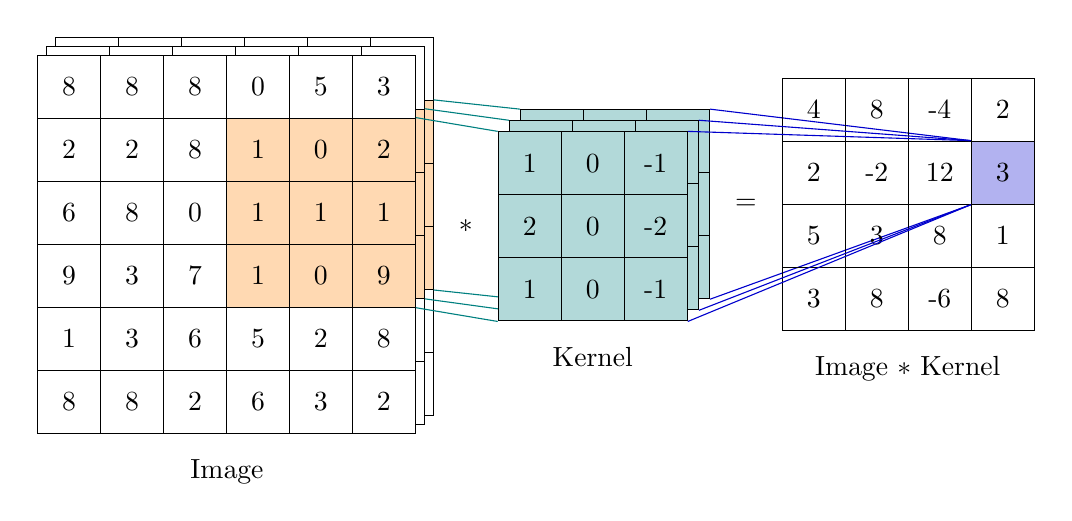
\begin{tikzpicture}[
    2d-arr/.style={minimum size=0.8cm, matrix of nodes, row sep=-\pgflinewidth, column sep=-\pgflinewidth, nodes={draw}}
  ]

  \begin{pgfonlayer}{foreground}
      \matrix (mtr) [2d-arr] {
      |[fill=white]| 8 & |[fill=white]| 8 & |[fill=white]| 8 & |[fill=white]| 0 & |[fill=white]| 5 & |[fill=white]| 3\\
      |[fill=white]| 2 & |[fill=white]| 2 & |[fill=white]| 8 & |[fill=orange!30]| 1 & |[fill=orange!30]| 0 & |[fill=orange!30]| 2\\
      |[fill=white]| 6 & |[fill=white]| 8 & |[fill=white]| 0 & |[fill=orange!30]| 1 & |[fill=orange!30]| 1 & |[fill=orange!30]| 1\\
      |[fill=white]| 9 & |[fill=white]| 3 & |[fill=white]| 7 & |[fill=orange!30]| 1 & |[fill=orange!30]| 0 & |[fill=orange!30]| 9\\
      |[fill=white]| 1 & |[fill=white]| 3 & |[fill=white]| 6 & |[fill=white]| 5 & |[fill=white]| 2 & |[fill=white]| 8\\
      |[fill=white]| 8 & |[fill=white]| 8 & |[fill=white]| 2 & |[fill=white]| 6 & |[fill=white]| 3 & |[fill=white]| 2\\
      };
  \end{pgfonlayer}

  \begin{pgfonlayer}{main}
      \matrix (mtr2) [2d-arr, above right=-7 cm of mtr] {
          |[fill=white]| 1 & |[fill=white]| 1 & |[fill=white]| 1 & |[fill=white]| 0 & |[fill=white]| 0 & |[fill=white]| 0\\
          |[fill=white]| 0 & |[fill=white]| 1 & |[fill=white]| 1 & |[fill=orange!30]| 1 & |[fill=orange!30]| 0 & |[fill=orange!30]| 0\\
          |[fill=white]| 0 & |[fill=white]| 0 & |[fill=white]| 1 & |[fill=orange!30]| 1 & |[fill=orange!30]| 1 & |[fill=orange!30]| 0\\
          |[fill=white]| 0 & |[fill=white]| 0 & |[fill=white]| 1 & |[fill=orange!30]| 1 & |[fill=orange!30]| 0 & |[fill=orange!30]| 0\\
          |[fill=white]| 0 & |[fill=white]| 1 & |[fill=white]| 1 & |[fill=white]| 0 & |[fill=white]| 0 & |[fill=white]| 0\\
          |[fill=white]| 1 & |[fill=white]| 1 & |[fill=white]| 0 & |[fill=white]| 0 & |[fill=white]| 0 & |[fill=white]| 0\\
      };
    \end{pgfonlayer}

  \begin{pgfonlayer}{background}
      \matrix (mtr3) [2d-arr, above right=-7 cm of mtr2] {
          |[fill=white]| 1 & |[fill=white]| 1 & |[fill=white]| 1 & |[fill=white]| 0 & |[fill=white]| 0 & |[fill=white]| 0\\
          |[fill=white]| 0 & |[fill=white]| 1 & |[fill=white]| 1 & |[fill=orange!30]| 1 & |[fill=orange!30]| 0 & |[fill=orange!30]| 0\\
          |[fill=white]| 0 & |[fill=white]| 0 & |[fill=white]| 1 & |[fill=orange!30]| 1 & |[fill=orange!30]| 1 & |[fill=orange!30]| 0\\
          |[fill=white]| 0 & |[fill=white]| 0 & |[fill=white]| 1 & |[fill=orange!30]| 1 & |[fill=orange!30]| 0 & |[fill=orange!30]| 0\\
          |[fill=white]| 0 & |[fill=white]| 1 & |[fill=white]| 1 & |[fill=white]| 0 & |[fill=white]| 0 & |[fill=white]| 0\\
          |[fill=white]| 1 & |[fill=white]| 1 & |[fill=white]| 0 & |[fill=white]| 0 & |[fill=white]| 0 & |[fill=white]| 0\\
      };
    \end{pgfonlayer}

  \node[below=of mtr-5-3.south east] {Image};

  \node[right=0.2em of mtr3] (str) {$*$};

  \begin{pgfonlayer}{foreground}
  \matrix (K) [2d-arr, right=0.2em of str, nodes={draw, fill=teal!30}] {
    1 & 0 & -1 \\
    2 & 0 & -2 \\
    1 & 0 & -1 \\
  };
  \end{pgfonlayer}

  \begin{pgfonlayer}{main}
  \matrix (K2) [2d-arr, below left=-3.965cm of K, nodes={draw, fill=teal!30}] {
    1 & 0 & 1 \\
    0 & 1 & 0 \\
    1 & 0 & 1 \\
  };
  \end{pgfonlayer}

  \begin{pgfonlayer}{background}
  \matrix (K3) [2d-arr, below left=-3.965cm of K2, nodes={draw, fill=teal!30}] {
    1 & 0 & 1 \\
    0 & 1 & 0 \\
    1 & 0 & 1 \\
  };
  \end{pgfonlayer}

  \node[below=of K-2-2] {Kernel};

  \node[right=0.2em of K3] (eq) {$=$};

  \matrix (ret) [2d-arr, right=0.2em of eq] {
  4 & 8 & -4 & 2\\
  2 & -2 & 12 & |[fill=blue!80!black!30]| 3\\
  5 & 3 & 8 & 1\\
  3 & 8 & -6 & 8\\
  };
  \node[below=of ret-3-3.south west] {Image $*$ Kernel};

  \begin{pgfonlayer}{foreground}
      \draw[teal] (mtr-4-6.south east) -- (K-3-1.south west);
      \draw[teal] (mtr-2-6.north east) -- (K-1-1.north west);

      \draw[blue!80!black] (K-1-3.north east) -- (ret-2-4.north west);
      \draw[blue!80!black] (K-3-3.south east) -- (ret-2-4.south west);
  \end{pgfonlayer}

  \begin{pgfonlayer}{main}
      \draw[teal] (mtr2-4-6.south east) -- (K2-3-1.south west);
      \draw[teal] (mtr2-2-6.north east) -- (K2-1-1.north west);

      \draw[blue!80!black] (K2-1-3.north east) -- (ret-2-4.north west);
      \draw[blue!80!black] (K2-3-3.south east) -- (ret-2-4.south west);
  \end{pgfonlayer}

  \begin{pgfonlayer}{background}
      \draw[teal] (mtr3-4-6.south east) -- (K3-3-1.south west);
      \draw[teal] (mtr3-2-6.north east) -- (K3-1-1.north west);

      \draw[blue!80!black] (K3-1-3.north east) -- (ret-2-4.north west);
      \draw[blue!80!black] (K3-3-3.south east) -- (ret-2-4.south west);
  \end{pgfonlayer}


\end{tikzpicture}

    \end{center}
    \caption[Convolution example]{Figure showing a convolutional kernel applied to a 3-channel image.}
    \label{fig:conv}
\end{figure}

By using several different kernels, we can detect many different patterns despite each kernel only detecting a single type. By using the outputs of all the kernels as inputs to a new set of kernels, we can use the same type layer structure as in an \ac{ffnn}, allowing us to extract information in a hierarchical manner. It is common to see that trained \acp{cnn} have early layers that detect edges and texture, later layers that use these edge and pattern detections to detect larger shapes, while the final layers combine the shapes to detect entire objects \cite{lenet5}.

By not evaluating every possible position in the input image, \acp{cnn} downsample the image, and are able to reduce the number of operations considerably. Simultaneously, this downsampling enables each subsequent layer to consider a larger area of the input image than the previous (a larger field-of-view), which allows larger patterns to be discovered. Simultaneously, it is common to use a larger and larger amounts of kernels on the new input, thus increasing the channel depth while the spatial dimensions are reduced. Between each layer, we use non-linear activation functions, similarly to how the are used in \acp{ffnn}.

After several such convolutions, we can flatten the output, either by aggregating each channel using \ac{gap} or a similar method, or we can simply flatten all dimensions and consider the three dimensional feature map as a long vector of shape $C \times H \times W$. By doing this, we can pass the output to one or more linear layers, which can perform classification or regression on the extracted features and give us a final prediction. Figure \ref{fig:cnn2} shows a high level overview of this process. Here, the input, which has only 3 channels, has its spatial dimensions reduced while its channel depth increases through consecutive convolutions. Finally, we have a certain number of channels in our final feature map, which are flattened (in this case with \ac{gap}) and processed through a linear layer to give a final prediction.


\begin{figure}[H]
    \begin{center}
    \end{center}


    \newcommand{\drawRectangles}[5]{
    % #1: Starting x-coordinate
    % #2: Starting y-coordinate (top)
    % #3: Rectangle size
    % #4: Spacing between rectangles
    % #5: Number of rectangles


    % Loop to draw rectangles
    \foreach \i in {0, 1, ..., \the\numexpr#5-1} {
        % Calculate x-coordinate for the current rectangle
        \pgfmathsetmacro{\x}{#1 + \i * #4)}
        \pgfmathsetmacro{\y}{#2 - \i * #4)}
        
        \pgfmathsetmacro{\fillColor}{mod(\i, 2) ? "ce0e0e0" : "ca0a0a0"}
        
        % Draw the rectangle
        \path[draw=black, fill=\fillColor, opacity=1, line width=0.0cm] 
            (\x, \y) rectangle (\x + #3, \y - #3);
    }
}


\def \globalscale {0.7}
\begin{tikzpicture}[y=1cm, x=1cm, yscale=\globalscale,xscale=\globalscale, every node/.append, inner sep=0pt, outer sep=0pt]
  \begin{scope}[shift={(3.5, 0.3)}]
    \path[draw=black,fill=red!20,opacity=1, line width=0.0cm] (12.6, 16.2) 
  rectangle (18.6, 10.3);
    \path[draw=black,fill=green!20,opacity=1, line width=0.0cm] (12.7, 16.1) 
  rectangle (18.7, 10.2);
    \path[draw=black,fill=blue!20,opacity=1, line width=0.0cm] (12.8, 16) 
  rectangle (18.8, 10.1);

    \begin{scope}[shift={(14, 11)}]
        \marmot[scale=1.3, body=blue]
        \bear[xshift=2.4cm, yshift=2.5cm, body=blue]
        \coati[rotatehead=-15, xshift=2.6cm, yshift=-0.5cm, body=blue]
    \end{scope}

    \drawRectangles{19.9}{15.0}{3.0}{0.1}{8}

    \drawRectangles{23.9}{14.8}{1.5}{0.12}{16}

    \drawRectangles{26.9}{15.3}{0.4}{0.133}{32}



    \path[draw=black,fill,fill opacity=0.0,draw opacity=1, line width=0.2mm] 
  (16.4, 14.3) rectangle (16.6, 14.1);
    \path[draw=black,fill,fill opacity=0.0,draw opacity=1, line width=0.2mm] 
  (21.3, 12.4) rectangle (21.7, 12.0);
    \path[draw=black,fill,fill opacity=0.0,draw opacity=1, line width=0.2mm] 
  (26.2, 11.9) rectangle (26.4, 11.7);

    \path[draw=black,fill,draw opacity=1, line width=0.2mm] (16.6, 14.1) -- 
  (22.6, 13.3);
    \path[draw=black,fill,draw opacity=1, line width=0.2mm] (16.6, 14.3) -- 
  (22.6, 13.3);
    \path[draw=black,fill,draw opacity=1, line width=0.2mm] (21.7, 12.0) -- 
  (26.2, 11.8);
    \path[draw=black,fill,draw opacity=1, line width=0.2mm] (21.7, 12.4) -- 
  (26.2, 11.8);
    \path[draw=black,fill,draw opacity=1, line width=0.2mm] (26.4, 11.7) -- 
  (31.1, 11.0);
    \path[draw=black,fill,draw opacity=1, line width=0.2mm] (26.4, 11.9) -- 
  (31.1, 11.0);

    \path[draw=black,fill=ce0e0e0,opacity=1, line width=0.0mm] (30.8, 13.5) -- 
  (31.1, 13.5) -- (32.0, 12.6) -- (31.7, 12.6) -- (30.8, 13.5)-- cycle;;
    \path[draw=black,fill=ce0e0e0,opacity=1, line width=0.0mm] (32.0, 13.2) -- 
  (32.3, 13.2) -- (32.6, 12.9) -- (32.3, 12.9) -- (32.0, 13.2)-- cycle;;

    \path[draw=black,fill,draw opacity=1, line width=0.2mm] (31.41, 11.15) -- 
  (31.7, 12.6);
    \path[draw=black,fill,draw opacity=1, line width=0.2mm] (27.3, 15.3) -- 
  (30.8, 13.5);
    \path[draw=black,fill,draw opacity=1, line width=0.2mm] (32.0, 12.6) -- 
  (32.3, 12.9);
    \path[draw=black,fill,draw opacity=1, line width=0.2mm] (31.1, 13.5) -- 
  (32.0, 13.2);


    \node[anchor=south west] (text10) at (19.9, 10.0){Conv};
    \node[anchor=south west] (text11) at (24.3, 10.0){Conv};
    \node[anchor=south west] (text12) at (27.9, 10.0){Conv};
    \node[anchor=south west] (text13) at (31.9, 11.0){GAP};
    \node[anchor=south west, align=left] (text14) at (12.6, 16.5){Input RGB Image:\\3@224x224};
    \node[anchor=south west] (text15) at (19.9, 15.4){8@112x112};
    \node[anchor=south west] (text16) at (23.9, 15.2){16@56x56};
    \node[anchor=south west] (text17) at (26.9, 15.7){32@14x14};
    \node[anchor=south west] (text18) at (30.8, 13.9){1x32};
    \node[anchor=south west] (text19) at (32.0, 13.6){1x10};
  \end{scope}



\end{tikzpicture}

    \caption[CNN example]{Figure showing a high level overview of how a CNN functions}
    \label{fig:cnn2}
\end{figure}


% \begin{figure}[H]
%     \begin{center}
%
%
%     \begin{tikzpicture}[x={(1,0)},y={(0,1)},z={({cos(60)},{sin(60)})}, scale=1.5]
% %
% % comment these out if you want to see where the axes point to
% % \draw[-latex] (0,0,0) -- (3,0,0) node[below]{$x$};
% % \draw[-latex] (0,0,0) -- (0,3,0) node[left]{$y$};
% % \draw[-latex] (0,0,0) -- (0,0,3) node[below]{$z$};
% % a plane
% \draw pic (box1-1) at (1,-1.6/2,0) {fake box=white!70!gray with dimensions {1/1.6/1.6} and {2*1.6} and {1*1.6} and Input};
%
% \foreach \X [count=\Y] in {1.4,1.2,1.2,1}
% {
%     \draw pic (box1-\Y) at (\Y+1,-\X/2,0) {fake box=white!70!gray with dimensions {1/\X/\X} and {2*\X} and {1*\X} and Conv};
% }
%
% \foreach \X/\Col in {6.5/blue,6.7/red,6.9/lightgray, 7.1/lightgray, 7.3/green}
% {\draw[canvas is yz plane at x = \X, transform shape, fill =
% \Col!50!white] (0,0.10) rectangle (1,-0.5);}
% % \draw[gray!60,thick] (6.3,-0.1,-1.6) coordinate (1-1) -- (6.3,-0.1,0.6) coordinate (1-2) -- (6.3,2.,0.6) coordinate (1-3) -- (6.3,2.1,-1.6) coordinate (1-4) -- cycle;
% % \draw[gray!60,thick] (7.1,-0.1,-1.6) coordinate (2-1) -- (7.1,-0.1,0.6) coordinate (2-2) -- (7.1,2.,0.6) coordinate (2-3) -- (7.1,2.1,-1.6) coordinate (2-4) -- cycle;
% % \foreach \X in {4,1,3}
% % {\draw[gray!60,thick] (1-\X) -- (2-\X);}
% %
% \node[draw,single arrow, fill=blue!10] at (8,0.5,0) {GAP};
% \node[circle,draw,blue,fill=blue!30] (A1) at (9,1,0) {~~~};
% \node[circle,draw,red,fill=red!30,below=4pt of A1] (A2) {~~~};
% \node[circle,draw,green,fill=green!30,below=18pt of A2] (A3) {~~~};
% \draw[circle dotted, line width=2pt,shorten <=3pt] (A2) -- (A3);
% \node[circle,draw,gray,fill=gray!20] (B1) at (10,1,0) {~~~};
% \node[circle,draw,fill=gray!60,below=4pt of B1] (B2) {~~~};
% \node[circle,draw,gray,fill=gray!20,below=18pt of B2] (B3) {~~~};
% \draw[circle dotted, line width=2pt,shorten <=3pt] (B2) -- (B3);
% \begin{scope}[on background layer]
% \node[orange,thick,rounded corners,fill=blue!10,fit=(A1) (A3)]{};
% \node[gray,thick,rounded corners,fill=gray!10,fit=(B1) (B3)]{};
% \end{scope}
% \foreach \X in {1,2,3}
% {\draw[-latex] (A\X) -- (B2);}
% \end{tikzpicture}
%
%     \end{center}
%     \caption[CNN example]{Figure showing a high level overview of how a CNN functions}
%     \label{fig:cnn2}
% \end{figure}

\section{Model evaluation}

\subsection{Metrics}

\ac{ood} detection is essentially simply a binary classification problem. Thus, the metrics I will use in this thesis are those used for such problems. In the field of \ac{ood} detection, \ac{auroc} and \ac{fpr} are most commonly used. As such I shall focus on these metrics, as opposed to for example the \ac{aupr}.

\subsubsection{Accuracy}

Accuracy is the simplest metric used in binary classification. It is simply the ratio of correct predictions over all instances in the data set. %, as seen in equation \ref{accuracy} below.

% \begin{equation}
% \text{accuracy} = \frac{TP + TN}{TP + TN + FP + FN}
% \label{eq:accuracy}
% \end{equation}

Accuracy has the advantage of being simple to understand and calculate, but it is very often insufficient. A simple (and quite common) scenario where accuracy fails to capture the performance of a model is any situation where there are large class imbalances. For example, imagine we have trained a \ac{cnn} to predict whether a person has lung cancer or not, based on CT-scans of their lungs. As most people do not have lung cancer, we can imagine that such a dataset is highly imbalanced, for example that only 1 in 100 people actually have cancer. If a model simply predicts that no one ever has lung cancer, it will be correct in $99\%$ of cases, and will thus have an accuracy of $99\%$, although it has missed every instance of cancer and is completely unusable in any real context.

For the purposes of \ac{ood} detection, accuracy is thus insufficient, as we have no guarantees that ID and OOD will be balanced. In fact, we expect OOD data to be relatively rare, given that the goal of developing an \ac{ai} model is to ensure high performance during deployment, which necessitates having training data which covers as much as possible of the data seen during inference.

\subsubsection{Metrics utilizing the binary classification confusion matrix} \label{section:aurocfpr95}

Instead of simply considering whether a prediction was correct or not, we should take into account the different combinations of prediction and ground truth, considering positive and negative classes separately. Figure \ref{fig:confusion} shows the possible four possible combinations given a ground truth class and a predicted class.

\begin{figure}[H]
    \begin{center}

    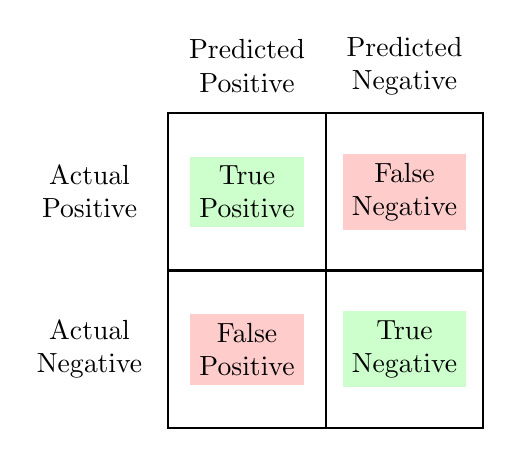
\begin{tikzpicture}
            % Draw the grid
    \draw[thick] (0,0) rectangle (4,4);
    \draw[thick] (2,0) -- (2,4);
    \draw[thick] (0,2) -- (4,2);

    % Label the axes
    \node[align=center] at (1,4.6) {Predicted\\Positive};
    \node[align=center] at (3,4.6) {Predicted\\Negative};

    \node[align=center] at (-1, 3) {Actual\\Positive};
    \node[align=center] at (-1, 1) {Actual\\Negative};

    % Label the cells
    \node[align=center, fill=green!20] at (1,3) {True\\Positive};
    \node[align=center, fill=red!20] at (1,1) {False\\Positive};
    \node[align=center, fill=red!20] at (3,3) {False\\Negative};
    \node[align=center, fill=green!20] at (3,1) {True\\Negative};
    \end{tikzpicture}

\end{center}
    \caption[Binary classification confusion matrix]{Figure showing the binary classification confusion matrix, denoting the four possible combinations created by the ground truth and predicted class. Green cells denote correct predictions, while red cells denote wrong predictions.}
\label{fig:confusion}
\end{figure}

With these possibilities defined, we can begin to gain a clearer picture of the performance of a model.

\noindent \textbf{Precision and Recall}

\noindent Precision is the share of positive predictions that were actually positive. With a high false positive rate, we have a low precision, which means that the model is erroneously flagging many negative classes as positive. In an \ac{ood} detection setting, a model which flags many ID samples as \ac{ood} would have a low precision, if we treat \ac{ood} samples as the positive class.

Recall is the share of actual positive samples that were predicted positive. Recall tells us how many of positive samples we missed. In and \ac{ood} detection context, a model which lets many \ac{ood} samples slip by undetected will have a low recall score.

Precision and recall are often used together because evaluate the model in different ways that complement each other. If a model has both high precision and high recall, it does not erroneously flag many negative classes as positive, nor does it miss many positive classes.

\noindent \textbf{Sensitivity and Specificity}

\noindent Sensitivity and specificity is another pair of metrics that is commonly used for evaluating binary classification. Sensitivity is equivalent to recall; the share of positive samples that were correctly predicted as positive. Specificity is the share of the negative samples that were correctly predicted as negative. Sensitivity and specificity are also known as \ac{tpr} and {\it True Negative Rate}.

\subsubsection{Threshold Independent Metrics}

The previous metrics are a clear improvement over simply using accuracy. However, they still have the problem that they are all dependent on what threshold one sets when predicting something to be a negative or positive class. Thus, it becomes harder to compare different models by using these metrics. Indeed, by simply increasing the threshold of any classifier, we can increase the true negative rate. Similarly, by decreasing the threshold, we can increase the true positive rate.\\

\noindent \textbf{Area under Receiver Operating Characteristic}:

\noindent \ac{auroc} remedies this problem by looking at all possible thresholds, and calculating the \ac{tpr} (equivalent to sensitivity, recall), and the \ac{fpr} (equivalent to $1 -$ specificity) for each possible threshold. With these values calculated, we can plot each point on a graph, giving us an \ac{roc} plot. Figure \ref{fig:auroc} shows this plot, for three different models.

\begin{figure}[H]
    \begin{center}
        %% Creator: Matplotlib, PGF backend
%%
%% To include the figure in your LaTeX document, write
%%   \input{<filename>.pgf}
%%
%% Make sure the required packages are loaded in your preamble
%%   \usepackage{pgf}
%%
%% Also ensure that all the required font packages are loaded; for instance,
%% the lmodern package is sometimes necessary when using math font.
%%   \usepackage{lmodern}
%%
%% Figures using additional raster images can only be included by \input if
%% they are in the same directory as the main LaTeX file. For loading figures
%% from other directories you can use the `import` package
%%   \usepackage{import}
%%
%% and then include the figures with
%%   \import{<path to file>}{<filename>.pgf}
%%
%% Matplotlib used the following preamble
%%   \def\mathdefault#1{#1}
%%   \everymath=\expandafter{\the\everymath\displaystyle}
%%   \IfFileExists{scrextend.sty}{
%%     \usepackage[fontsize=10.000000pt]{scrextend}
%%   }{
%%     \renewcommand{\normalsize}{\fontsize{10.000000}{12.000000}\selectfont}
%%     \normalsize
%%   }
%%   
%%   \makeatletter\@ifpackageloaded{underscore}{}{\usepackage[strings]{underscore}}\makeatother
%%
\begingroup%
\makeatletter%
\begin{pgfpicture}%
\pgfpathrectangle{\pgfpointorigin}{\pgfqpoint{6.400000in}{4.800000in}}%
\pgfusepath{use as bounding box, clip}%
\begin{pgfscope}%
\pgfsetbuttcap%
\pgfsetmiterjoin%
\definecolor{currentfill}{rgb}{1.000000,1.000000,1.000000}%
\pgfsetfillcolor{currentfill}%
\pgfsetlinewidth{0.000000pt}%
\definecolor{currentstroke}{rgb}{1.000000,1.000000,1.000000}%
\pgfsetstrokecolor{currentstroke}%
\pgfsetdash{}{0pt}%
\pgfpathmoveto{\pgfqpoint{0.000000in}{0.000000in}}%
\pgfpathlineto{\pgfqpoint{6.400000in}{0.000000in}}%
\pgfpathlineto{\pgfqpoint{6.400000in}{4.800000in}}%
\pgfpathlineto{\pgfqpoint{0.000000in}{4.800000in}}%
\pgfpathlineto{\pgfqpoint{0.000000in}{0.000000in}}%
\pgfpathclose%
\pgfusepath{fill}%
\end{pgfscope}%
\begin{pgfscope}%
\pgfsetbuttcap%
\pgfsetmiterjoin%
\definecolor{currentfill}{rgb}{1.000000,1.000000,1.000000}%
\pgfsetfillcolor{currentfill}%
\pgfsetlinewidth{0.000000pt}%
\definecolor{currentstroke}{rgb}{0.000000,0.000000,0.000000}%
\pgfsetstrokecolor{currentstroke}%
\pgfsetstrokeopacity{0.000000}%
\pgfsetdash{}{0pt}%
\pgfpathmoveto{\pgfqpoint{0.800000in}{0.528000in}}%
\pgfpathlineto{\pgfqpoint{5.760000in}{0.528000in}}%
\pgfpathlineto{\pgfqpoint{5.760000in}{4.224000in}}%
\pgfpathlineto{\pgfqpoint{0.800000in}{4.224000in}}%
\pgfpathlineto{\pgfqpoint{0.800000in}{0.528000in}}%
\pgfpathclose%
\pgfusepath{fill}%
\end{pgfscope}%
\begin{pgfscope}%
\pgfpathrectangle{\pgfqpoint{0.800000in}{0.528000in}}{\pgfqpoint{4.960000in}{3.696000in}}%
\pgfusepath{clip}%
\pgfsetrectcap%
\pgfsetroundjoin%
\pgfsetlinewidth{0.803000pt}%
\definecolor{currentstroke}{rgb}{0.690196,0.690196,0.690196}%
\pgfsetstrokecolor{currentstroke}%
\pgfsetdash{}{0pt}%
\pgfpathmoveto{\pgfqpoint{0.800000in}{0.528000in}}%
\pgfpathlineto{\pgfqpoint{0.800000in}{4.224000in}}%
\pgfusepath{stroke}%
\end{pgfscope}%
\begin{pgfscope}%
\pgfsetbuttcap%
\pgfsetroundjoin%
\definecolor{currentfill}{rgb}{0.000000,0.000000,0.000000}%
\pgfsetfillcolor{currentfill}%
\pgfsetlinewidth{0.803000pt}%
\definecolor{currentstroke}{rgb}{0.000000,0.000000,0.000000}%
\pgfsetstrokecolor{currentstroke}%
\pgfsetdash{}{0pt}%
\pgfsys@defobject{currentmarker}{\pgfqpoint{0.000000in}{-0.048611in}}{\pgfqpoint{0.000000in}{0.000000in}}{%
\pgfpathmoveto{\pgfqpoint{0.000000in}{0.000000in}}%
\pgfpathlineto{\pgfqpoint{0.000000in}{-0.048611in}}%
\pgfusepath{stroke,fill}%
}%
\begin{pgfscope}%
\pgfsys@transformshift{0.800000in}{0.528000in}%
\pgfsys@useobject{currentmarker}{}%
\end{pgfscope}%
\end{pgfscope}%
\begin{pgfscope}%
\definecolor{textcolor}{rgb}{0.000000,0.000000,0.000000}%
\pgfsetstrokecolor{textcolor}%
\pgfsetfillcolor{textcolor}%
\pgftext[x=0.800000in,y=0.430778in,,top]{\color{textcolor}{\rmfamily\fontsize{10.000000}{12.000000}\selectfont\catcode`\^=\active\def^{\ifmmode\sp\else\^{}\fi}\catcode`\%=\active\def%{\%}$\mathdefault{0.0}$}}%
\end{pgfscope}%
\begin{pgfscope}%
\pgfpathrectangle{\pgfqpoint{0.800000in}{0.528000in}}{\pgfqpoint{4.960000in}{3.696000in}}%
\pgfusepath{clip}%
\pgfsetrectcap%
\pgfsetroundjoin%
\pgfsetlinewidth{0.803000pt}%
\definecolor{currentstroke}{rgb}{0.690196,0.690196,0.690196}%
\pgfsetstrokecolor{currentstroke}%
\pgfsetdash{}{0pt}%
\pgfpathmoveto{\pgfqpoint{1.792000in}{0.528000in}}%
\pgfpathlineto{\pgfqpoint{1.792000in}{4.224000in}}%
\pgfusepath{stroke}%
\end{pgfscope}%
\begin{pgfscope}%
\pgfsetbuttcap%
\pgfsetroundjoin%
\definecolor{currentfill}{rgb}{0.000000,0.000000,0.000000}%
\pgfsetfillcolor{currentfill}%
\pgfsetlinewidth{0.803000pt}%
\definecolor{currentstroke}{rgb}{0.000000,0.000000,0.000000}%
\pgfsetstrokecolor{currentstroke}%
\pgfsetdash{}{0pt}%
\pgfsys@defobject{currentmarker}{\pgfqpoint{0.000000in}{-0.048611in}}{\pgfqpoint{0.000000in}{0.000000in}}{%
\pgfpathmoveto{\pgfqpoint{0.000000in}{0.000000in}}%
\pgfpathlineto{\pgfqpoint{0.000000in}{-0.048611in}}%
\pgfusepath{stroke,fill}%
}%
\begin{pgfscope}%
\pgfsys@transformshift{1.792000in}{0.528000in}%
\pgfsys@useobject{currentmarker}{}%
\end{pgfscope}%
\end{pgfscope}%
\begin{pgfscope}%
\definecolor{textcolor}{rgb}{0.000000,0.000000,0.000000}%
\pgfsetstrokecolor{textcolor}%
\pgfsetfillcolor{textcolor}%
\pgftext[x=1.792000in,y=0.430778in,,top]{\color{textcolor}{\rmfamily\fontsize{10.000000}{12.000000}\selectfont\catcode`\^=\active\def^{\ifmmode\sp\else\^{}\fi}\catcode`\%=\active\def%{\%}$\mathdefault{0.2}$}}%
\end{pgfscope}%
\begin{pgfscope}%
\pgfpathrectangle{\pgfqpoint{0.800000in}{0.528000in}}{\pgfqpoint{4.960000in}{3.696000in}}%
\pgfusepath{clip}%
\pgfsetrectcap%
\pgfsetroundjoin%
\pgfsetlinewidth{0.803000pt}%
\definecolor{currentstroke}{rgb}{0.690196,0.690196,0.690196}%
\pgfsetstrokecolor{currentstroke}%
\pgfsetdash{}{0pt}%
\pgfpathmoveto{\pgfqpoint{2.784000in}{0.528000in}}%
\pgfpathlineto{\pgfqpoint{2.784000in}{4.224000in}}%
\pgfusepath{stroke}%
\end{pgfscope}%
\begin{pgfscope}%
\pgfsetbuttcap%
\pgfsetroundjoin%
\definecolor{currentfill}{rgb}{0.000000,0.000000,0.000000}%
\pgfsetfillcolor{currentfill}%
\pgfsetlinewidth{0.803000pt}%
\definecolor{currentstroke}{rgb}{0.000000,0.000000,0.000000}%
\pgfsetstrokecolor{currentstroke}%
\pgfsetdash{}{0pt}%
\pgfsys@defobject{currentmarker}{\pgfqpoint{0.000000in}{-0.048611in}}{\pgfqpoint{0.000000in}{0.000000in}}{%
\pgfpathmoveto{\pgfqpoint{0.000000in}{0.000000in}}%
\pgfpathlineto{\pgfqpoint{0.000000in}{-0.048611in}}%
\pgfusepath{stroke,fill}%
}%
\begin{pgfscope}%
\pgfsys@transformshift{2.784000in}{0.528000in}%
\pgfsys@useobject{currentmarker}{}%
\end{pgfscope}%
\end{pgfscope}%
\begin{pgfscope}%
\definecolor{textcolor}{rgb}{0.000000,0.000000,0.000000}%
\pgfsetstrokecolor{textcolor}%
\pgfsetfillcolor{textcolor}%
\pgftext[x=2.784000in,y=0.430778in,,top]{\color{textcolor}{\rmfamily\fontsize{10.000000}{12.000000}\selectfont\catcode`\^=\active\def^{\ifmmode\sp\else\^{}\fi}\catcode`\%=\active\def%{\%}$\mathdefault{0.4}$}}%
\end{pgfscope}%
\begin{pgfscope}%
\pgfpathrectangle{\pgfqpoint{0.800000in}{0.528000in}}{\pgfqpoint{4.960000in}{3.696000in}}%
\pgfusepath{clip}%
\pgfsetrectcap%
\pgfsetroundjoin%
\pgfsetlinewidth{0.803000pt}%
\definecolor{currentstroke}{rgb}{0.690196,0.690196,0.690196}%
\pgfsetstrokecolor{currentstroke}%
\pgfsetdash{}{0pt}%
\pgfpathmoveto{\pgfqpoint{3.776000in}{0.528000in}}%
\pgfpathlineto{\pgfqpoint{3.776000in}{4.224000in}}%
\pgfusepath{stroke}%
\end{pgfscope}%
\begin{pgfscope}%
\pgfsetbuttcap%
\pgfsetroundjoin%
\definecolor{currentfill}{rgb}{0.000000,0.000000,0.000000}%
\pgfsetfillcolor{currentfill}%
\pgfsetlinewidth{0.803000pt}%
\definecolor{currentstroke}{rgb}{0.000000,0.000000,0.000000}%
\pgfsetstrokecolor{currentstroke}%
\pgfsetdash{}{0pt}%
\pgfsys@defobject{currentmarker}{\pgfqpoint{0.000000in}{-0.048611in}}{\pgfqpoint{0.000000in}{0.000000in}}{%
\pgfpathmoveto{\pgfqpoint{0.000000in}{0.000000in}}%
\pgfpathlineto{\pgfqpoint{0.000000in}{-0.048611in}}%
\pgfusepath{stroke,fill}%
}%
\begin{pgfscope}%
\pgfsys@transformshift{3.776000in}{0.528000in}%
\pgfsys@useobject{currentmarker}{}%
\end{pgfscope}%
\end{pgfscope}%
\begin{pgfscope}%
\definecolor{textcolor}{rgb}{0.000000,0.000000,0.000000}%
\pgfsetstrokecolor{textcolor}%
\pgfsetfillcolor{textcolor}%
\pgftext[x=3.776000in,y=0.430778in,,top]{\color{textcolor}{\rmfamily\fontsize{10.000000}{12.000000}\selectfont\catcode`\^=\active\def^{\ifmmode\sp\else\^{}\fi}\catcode`\%=\active\def%{\%}$\mathdefault{0.6}$}}%
\end{pgfscope}%
\begin{pgfscope}%
\pgfpathrectangle{\pgfqpoint{0.800000in}{0.528000in}}{\pgfqpoint{4.960000in}{3.696000in}}%
\pgfusepath{clip}%
\pgfsetrectcap%
\pgfsetroundjoin%
\pgfsetlinewidth{0.803000pt}%
\definecolor{currentstroke}{rgb}{0.690196,0.690196,0.690196}%
\pgfsetstrokecolor{currentstroke}%
\pgfsetdash{}{0pt}%
\pgfpathmoveto{\pgfqpoint{4.768000in}{0.528000in}}%
\pgfpathlineto{\pgfqpoint{4.768000in}{4.224000in}}%
\pgfusepath{stroke}%
\end{pgfscope}%
\begin{pgfscope}%
\pgfsetbuttcap%
\pgfsetroundjoin%
\definecolor{currentfill}{rgb}{0.000000,0.000000,0.000000}%
\pgfsetfillcolor{currentfill}%
\pgfsetlinewidth{0.803000pt}%
\definecolor{currentstroke}{rgb}{0.000000,0.000000,0.000000}%
\pgfsetstrokecolor{currentstroke}%
\pgfsetdash{}{0pt}%
\pgfsys@defobject{currentmarker}{\pgfqpoint{0.000000in}{-0.048611in}}{\pgfqpoint{0.000000in}{0.000000in}}{%
\pgfpathmoveto{\pgfqpoint{0.000000in}{0.000000in}}%
\pgfpathlineto{\pgfqpoint{0.000000in}{-0.048611in}}%
\pgfusepath{stroke,fill}%
}%
\begin{pgfscope}%
\pgfsys@transformshift{4.768000in}{0.528000in}%
\pgfsys@useobject{currentmarker}{}%
\end{pgfscope}%
\end{pgfscope}%
\begin{pgfscope}%
\definecolor{textcolor}{rgb}{0.000000,0.000000,0.000000}%
\pgfsetstrokecolor{textcolor}%
\pgfsetfillcolor{textcolor}%
\pgftext[x=4.768000in,y=0.430778in,,top]{\color{textcolor}{\rmfamily\fontsize{10.000000}{12.000000}\selectfont\catcode`\^=\active\def^{\ifmmode\sp\else\^{}\fi}\catcode`\%=\active\def%{\%}$\mathdefault{0.8}$}}%
\end{pgfscope}%
\begin{pgfscope}%
\pgfpathrectangle{\pgfqpoint{0.800000in}{0.528000in}}{\pgfqpoint{4.960000in}{3.696000in}}%
\pgfusepath{clip}%
\pgfsetrectcap%
\pgfsetroundjoin%
\pgfsetlinewidth{0.803000pt}%
\definecolor{currentstroke}{rgb}{0.690196,0.690196,0.690196}%
\pgfsetstrokecolor{currentstroke}%
\pgfsetdash{}{0pt}%
\pgfpathmoveto{\pgfqpoint{5.760000in}{0.528000in}}%
\pgfpathlineto{\pgfqpoint{5.760000in}{4.224000in}}%
\pgfusepath{stroke}%
\end{pgfscope}%
\begin{pgfscope}%
\pgfsetbuttcap%
\pgfsetroundjoin%
\definecolor{currentfill}{rgb}{0.000000,0.000000,0.000000}%
\pgfsetfillcolor{currentfill}%
\pgfsetlinewidth{0.803000pt}%
\definecolor{currentstroke}{rgb}{0.000000,0.000000,0.000000}%
\pgfsetstrokecolor{currentstroke}%
\pgfsetdash{}{0pt}%
\pgfsys@defobject{currentmarker}{\pgfqpoint{0.000000in}{-0.048611in}}{\pgfqpoint{0.000000in}{0.000000in}}{%
\pgfpathmoveto{\pgfqpoint{0.000000in}{0.000000in}}%
\pgfpathlineto{\pgfqpoint{0.000000in}{-0.048611in}}%
\pgfusepath{stroke,fill}%
}%
\begin{pgfscope}%
\pgfsys@transformshift{5.760000in}{0.528000in}%
\pgfsys@useobject{currentmarker}{}%
\end{pgfscope}%
\end{pgfscope}%
\begin{pgfscope}%
\definecolor{textcolor}{rgb}{0.000000,0.000000,0.000000}%
\pgfsetstrokecolor{textcolor}%
\pgfsetfillcolor{textcolor}%
\pgftext[x=5.760000in,y=0.430778in,,top]{\color{textcolor}{\rmfamily\fontsize{10.000000}{12.000000}\selectfont\catcode`\^=\active\def^{\ifmmode\sp\else\^{}\fi}\catcode`\%=\active\def%{\%}$\mathdefault{1.0}$}}%
\end{pgfscope}%
\begin{pgfscope}%
\definecolor{textcolor}{rgb}{0.000000,0.000000,0.000000}%
\pgfsetstrokecolor{textcolor}%
\pgfsetfillcolor{textcolor}%
\pgftext[x=3.280000in,y=0.251766in,,top]{\color{textcolor}{\rmfamily\fontsize{10.000000}{12.000000}\selectfont\catcode`\^=\active\def^{\ifmmode\sp\else\^{}\fi}\catcode`\%=\active\def%{\%}False Positive Rate (FPR)}}%
\end{pgfscope}%
\begin{pgfscope}%
\pgfpathrectangle{\pgfqpoint{0.800000in}{0.528000in}}{\pgfqpoint{4.960000in}{3.696000in}}%
\pgfusepath{clip}%
\pgfsetrectcap%
\pgfsetroundjoin%
\pgfsetlinewidth{0.803000pt}%
\definecolor{currentstroke}{rgb}{0.690196,0.690196,0.690196}%
\pgfsetstrokecolor{currentstroke}%
\pgfsetdash{}{0pt}%
\pgfpathmoveto{\pgfqpoint{0.800000in}{0.528000in}}%
\pgfpathlineto{\pgfqpoint{5.760000in}{0.528000in}}%
\pgfusepath{stroke}%
\end{pgfscope}%
\begin{pgfscope}%
\pgfsetbuttcap%
\pgfsetroundjoin%
\definecolor{currentfill}{rgb}{0.000000,0.000000,0.000000}%
\pgfsetfillcolor{currentfill}%
\pgfsetlinewidth{0.803000pt}%
\definecolor{currentstroke}{rgb}{0.000000,0.000000,0.000000}%
\pgfsetstrokecolor{currentstroke}%
\pgfsetdash{}{0pt}%
\pgfsys@defobject{currentmarker}{\pgfqpoint{-0.048611in}{0.000000in}}{\pgfqpoint{-0.000000in}{0.000000in}}{%
\pgfpathmoveto{\pgfqpoint{-0.000000in}{0.000000in}}%
\pgfpathlineto{\pgfqpoint{-0.048611in}{0.000000in}}%
\pgfusepath{stroke,fill}%
}%
\begin{pgfscope}%
\pgfsys@transformshift{0.800000in}{0.528000in}%
\pgfsys@useobject{currentmarker}{}%
\end{pgfscope}%
\end{pgfscope}%
\begin{pgfscope}%
\definecolor{textcolor}{rgb}{0.000000,0.000000,0.000000}%
\pgfsetstrokecolor{textcolor}%
\pgfsetfillcolor{textcolor}%
\pgftext[x=0.525308in, y=0.479775in, left, base]{\color{textcolor}{\rmfamily\fontsize{10.000000}{12.000000}\selectfont\catcode`\^=\active\def^{\ifmmode\sp\else\^{}\fi}\catcode`\%=\active\def%{\%}$\mathdefault{0.0}$}}%
\end{pgfscope}%
\begin{pgfscope}%
\pgfpathrectangle{\pgfqpoint{0.800000in}{0.528000in}}{\pgfqpoint{4.960000in}{3.696000in}}%
\pgfusepath{clip}%
\pgfsetrectcap%
\pgfsetroundjoin%
\pgfsetlinewidth{0.803000pt}%
\definecolor{currentstroke}{rgb}{0.690196,0.690196,0.690196}%
\pgfsetstrokecolor{currentstroke}%
\pgfsetdash{}{0pt}%
\pgfpathmoveto{\pgfqpoint{0.800000in}{1.267200in}}%
\pgfpathlineto{\pgfqpoint{5.760000in}{1.267200in}}%
\pgfusepath{stroke}%
\end{pgfscope}%
\begin{pgfscope}%
\pgfsetbuttcap%
\pgfsetroundjoin%
\definecolor{currentfill}{rgb}{0.000000,0.000000,0.000000}%
\pgfsetfillcolor{currentfill}%
\pgfsetlinewidth{0.803000pt}%
\definecolor{currentstroke}{rgb}{0.000000,0.000000,0.000000}%
\pgfsetstrokecolor{currentstroke}%
\pgfsetdash{}{0pt}%
\pgfsys@defobject{currentmarker}{\pgfqpoint{-0.048611in}{0.000000in}}{\pgfqpoint{-0.000000in}{0.000000in}}{%
\pgfpathmoveto{\pgfqpoint{-0.000000in}{0.000000in}}%
\pgfpathlineto{\pgfqpoint{-0.048611in}{0.000000in}}%
\pgfusepath{stroke,fill}%
}%
\begin{pgfscope}%
\pgfsys@transformshift{0.800000in}{1.267200in}%
\pgfsys@useobject{currentmarker}{}%
\end{pgfscope}%
\end{pgfscope}%
\begin{pgfscope}%
\definecolor{textcolor}{rgb}{0.000000,0.000000,0.000000}%
\pgfsetstrokecolor{textcolor}%
\pgfsetfillcolor{textcolor}%
\pgftext[x=0.525308in, y=1.218975in, left, base]{\color{textcolor}{\rmfamily\fontsize{10.000000}{12.000000}\selectfont\catcode`\^=\active\def^{\ifmmode\sp\else\^{}\fi}\catcode`\%=\active\def%{\%}$\mathdefault{0.2}$}}%
\end{pgfscope}%
\begin{pgfscope}%
\pgfpathrectangle{\pgfqpoint{0.800000in}{0.528000in}}{\pgfqpoint{4.960000in}{3.696000in}}%
\pgfusepath{clip}%
\pgfsetrectcap%
\pgfsetroundjoin%
\pgfsetlinewidth{0.803000pt}%
\definecolor{currentstroke}{rgb}{0.690196,0.690196,0.690196}%
\pgfsetstrokecolor{currentstroke}%
\pgfsetdash{}{0pt}%
\pgfpathmoveto{\pgfqpoint{0.800000in}{2.006400in}}%
\pgfpathlineto{\pgfqpoint{5.760000in}{2.006400in}}%
\pgfusepath{stroke}%
\end{pgfscope}%
\begin{pgfscope}%
\pgfsetbuttcap%
\pgfsetroundjoin%
\definecolor{currentfill}{rgb}{0.000000,0.000000,0.000000}%
\pgfsetfillcolor{currentfill}%
\pgfsetlinewidth{0.803000pt}%
\definecolor{currentstroke}{rgb}{0.000000,0.000000,0.000000}%
\pgfsetstrokecolor{currentstroke}%
\pgfsetdash{}{0pt}%
\pgfsys@defobject{currentmarker}{\pgfqpoint{-0.048611in}{0.000000in}}{\pgfqpoint{-0.000000in}{0.000000in}}{%
\pgfpathmoveto{\pgfqpoint{-0.000000in}{0.000000in}}%
\pgfpathlineto{\pgfqpoint{-0.048611in}{0.000000in}}%
\pgfusepath{stroke,fill}%
}%
\begin{pgfscope}%
\pgfsys@transformshift{0.800000in}{2.006400in}%
\pgfsys@useobject{currentmarker}{}%
\end{pgfscope}%
\end{pgfscope}%
\begin{pgfscope}%
\definecolor{textcolor}{rgb}{0.000000,0.000000,0.000000}%
\pgfsetstrokecolor{textcolor}%
\pgfsetfillcolor{textcolor}%
\pgftext[x=0.525308in, y=1.958175in, left, base]{\color{textcolor}{\rmfamily\fontsize{10.000000}{12.000000}\selectfont\catcode`\^=\active\def^{\ifmmode\sp\else\^{}\fi}\catcode`\%=\active\def%{\%}$\mathdefault{0.4}$}}%
\end{pgfscope}%
\begin{pgfscope}%
\pgfpathrectangle{\pgfqpoint{0.800000in}{0.528000in}}{\pgfqpoint{4.960000in}{3.696000in}}%
\pgfusepath{clip}%
\pgfsetrectcap%
\pgfsetroundjoin%
\pgfsetlinewidth{0.803000pt}%
\definecolor{currentstroke}{rgb}{0.690196,0.690196,0.690196}%
\pgfsetstrokecolor{currentstroke}%
\pgfsetdash{}{0pt}%
\pgfpathmoveto{\pgfqpoint{0.800000in}{2.745600in}}%
\pgfpathlineto{\pgfqpoint{5.760000in}{2.745600in}}%
\pgfusepath{stroke}%
\end{pgfscope}%
\begin{pgfscope}%
\pgfsetbuttcap%
\pgfsetroundjoin%
\definecolor{currentfill}{rgb}{0.000000,0.000000,0.000000}%
\pgfsetfillcolor{currentfill}%
\pgfsetlinewidth{0.803000pt}%
\definecolor{currentstroke}{rgb}{0.000000,0.000000,0.000000}%
\pgfsetstrokecolor{currentstroke}%
\pgfsetdash{}{0pt}%
\pgfsys@defobject{currentmarker}{\pgfqpoint{-0.048611in}{0.000000in}}{\pgfqpoint{-0.000000in}{0.000000in}}{%
\pgfpathmoveto{\pgfqpoint{-0.000000in}{0.000000in}}%
\pgfpathlineto{\pgfqpoint{-0.048611in}{0.000000in}}%
\pgfusepath{stroke,fill}%
}%
\begin{pgfscope}%
\pgfsys@transformshift{0.800000in}{2.745600in}%
\pgfsys@useobject{currentmarker}{}%
\end{pgfscope}%
\end{pgfscope}%
\begin{pgfscope}%
\definecolor{textcolor}{rgb}{0.000000,0.000000,0.000000}%
\pgfsetstrokecolor{textcolor}%
\pgfsetfillcolor{textcolor}%
\pgftext[x=0.525308in, y=2.697375in, left, base]{\color{textcolor}{\rmfamily\fontsize{10.000000}{12.000000}\selectfont\catcode`\^=\active\def^{\ifmmode\sp\else\^{}\fi}\catcode`\%=\active\def%{\%}$\mathdefault{0.6}$}}%
\end{pgfscope}%
\begin{pgfscope}%
\pgfpathrectangle{\pgfqpoint{0.800000in}{0.528000in}}{\pgfqpoint{4.960000in}{3.696000in}}%
\pgfusepath{clip}%
\pgfsetrectcap%
\pgfsetroundjoin%
\pgfsetlinewidth{0.803000pt}%
\definecolor{currentstroke}{rgb}{0.690196,0.690196,0.690196}%
\pgfsetstrokecolor{currentstroke}%
\pgfsetdash{}{0pt}%
\pgfpathmoveto{\pgfqpoint{0.800000in}{3.484800in}}%
\pgfpathlineto{\pgfqpoint{5.760000in}{3.484800in}}%
\pgfusepath{stroke}%
\end{pgfscope}%
\begin{pgfscope}%
\pgfsetbuttcap%
\pgfsetroundjoin%
\definecolor{currentfill}{rgb}{0.000000,0.000000,0.000000}%
\pgfsetfillcolor{currentfill}%
\pgfsetlinewidth{0.803000pt}%
\definecolor{currentstroke}{rgb}{0.000000,0.000000,0.000000}%
\pgfsetstrokecolor{currentstroke}%
\pgfsetdash{}{0pt}%
\pgfsys@defobject{currentmarker}{\pgfqpoint{-0.048611in}{0.000000in}}{\pgfqpoint{-0.000000in}{0.000000in}}{%
\pgfpathmoveto{\pgfqpoint{-0.000000in}{0.000000in}}%
\pgfpathlineto{\pgfqpoint{-0.048611in}{0.000000in}}%
\pgfusepath{stroke,fill}%
}%
\begin{pgfscope}%
\pgfsys@transformshift{0.800000in}{3.484800in}%
\pgfsys@useobject{currentmarker}{}%
\end{pgfscope}%
\end{pgfscope}%
\begin{pgfscope}%
\definecolor{textcolor}{rgb}{0.000000,0.000000,0.000000}%
\pgfsetstrokecolor{textcolor}%
\pgfsetfillcolor{textcolor}%
\pgftext[x=0.525308in, y=3.436575in, left, base]{\color{textcolor}{\rmfamily\fontsize{10.000000}{12.000000}\selectfont\catcode`\^=\active\def^{\ifmmode\sp\else\^{}\fi}\catcode`\%=\active\def%{\%}$\mathdefault{0.8}$}}%
\end{pgfscope}%
\begin{pgfscope}%
\pgfpathrectangle{\pgfqpoint{0.800000in}{0.528000in}}{\pgfqpoint{4.960000in}{3.696000in}}%
\pgfusepath{clip}%
\pgfsetrectcap%
\pgfsetroundjoin%
\pgfsetlinewidth{0.803000pt}%
\definecolor{currentstroke}{rgb}{0.690196,0.690196,0.690196}%
\pgfsetstrokecolor{currentstroke}%
\pgfsetdash{}{0pt}%
\pgfpathmoveto{\pgfqpoint{0.800000in}{4.224000in}}%
\pgfpathlineto{\pgfqpoint{5.760000in}{4.224000in}}%
\pgfusepath{stroke}%
\end{pgfscope}%
\begin{pgfscope}%
\pgfsetbuttcap%
\pgfsetroundjoin%
\definecolor{currentfill}{rgb}{0.000000,0.000000,0.000000}%
\pgfsetfillcolor{currentfill}%
\pgfsetlinewidth{0.803000pt}%
\definecolor{currentstroke}{rgb}{0.000000,0.000000,0.000000}%
\pgfsetstrokecolor{currentstroke}%
\pgfsetdash{}{0pt}%
\pgfsys@defobject{currentmarker}{\pgfqpoint{-0.048611in}{0.000000in}}{\pgfqpoint{-0.000000in}{0.000000in}}{%
\pgfpathmoveto{\pgfqpoint{-0.000000in}{0.000000in}}%
\pgfpathlineto{\pgfqpoint{-0.048611in}{0.000000in}}%
\pgfusepath{stroke,fill}%
}%
\begin{pgfscope}%
\pgfsys@transformshift{0.800000in}{4.224000in}%
\pgfsys@useobject{currentmarker}{}%
\end{pgfscope}%
\end{pgfscope}%
\begin{pgfscope}%
\definecolor{textcolor}{rgb}{0.000000,0.000000,0.000000}%
\pgfsetstrokecolor{textcolor}%
\pgfsetfillcolor{textcolor}%
\pgftext[x=0.525308in, y=4.175775in, left, base]{\color{textcolor}{\rmfamily\fontsize{10.000000}{12.000000}\selectfont\catcode`\^=\active\def^{\ifmmode\sp\else\^{}\fi}\catcode`\%=\active\def%{\%}$\mathdefault{1.0}$}}%
\end{pgfscope}%
\begin{pgfscope}%
\definecolor{textcolor}{rgb}{0.000000,0.000000,0.000000}%
\pgfsetstrokecolor{textcolor}%
\pgfsetfillcolor{textcolor}%
\pgftext[x=0.469752in,y=2.376000in,,bottom,rotate=90.000000]{\color{textcolor}{\rmfamily\fontsize{10.000000}{12.000000}\selectfont\catcode`\^=\active\def^{\ifmmode\sp\else\^{}\fi}\catcode`\%=\active\def%{\%}True Positive Rate (TPR)}}%
\end{pgfscope}%
\begin{pgfscope}%
\pgfpathrectangle{\pgfqpoint{0.800000in}{0.528000in}}{\pgfqpoint{4.960000in}{3.696000in}}%
\pgfusepath{clip}%
\pgfsetrectcap%
\pgfsetroundjoin%
\pgfsetlinewidth{1.505625pt}%
\definecolor{currentstroke}{rgb}{0.000000,0.501961,0.000000}%
\pgfsetstrokecolor{currentstroke}%
\pgfsetdash{}{0pt}%
\pgfpathmoveto{\pgfqpoint{0.800000in}{0.528000in}}%
\pgfpathlineto{\pgfqpoint{0.800000in}{0.564960in}}%
\pgfpathlineto{\pgfqpoint{0.800000in}{1.415040in}}%
\pgfpathlineto{\pgfqpoint{0.849600in}{1.415040in}}%
\pgfpathlineto{\pgfqpoint{0.849600in}{3.041280in}}%
\pgfpathlineto{\pgfqpoint{0.899200in}{3.041280in}}%
\pgfpathlineto{\pgfqpoint{0.899200in}{3.595680in}}%
\pgfpathlineto{\pgfqpoint{0.948800in}{3.595680in}}%
\pgfpathlineto{\pgfqpoint{0.948800in}{3.669600in}}%
\pgfpathlineto{\pgfqpoint{0.998400in}{3.669600in}}%
\pgfpathlineto{\pgfqpoint{0.998400in}{3.706560in}}%
\pgfpathlineto{\pgfqpoint{1.048000in}{3.706560in}}%
\pgfpathlineto{\pgfqpoint{1.048000in}{3.891360in}}%
\pgfpathlineto{\pgfqpoint{1.246400in}{3.891360in}}%
\pgfpathlineto{\pgfqpoint{1.246400in}{4.039200in}}%
\pgfpathlineto{\pgfqpoint{1.296000in}{4.039200in}}%
\pgfpathlineto{\pgfqpoint{1.296000in}{4.076160in}}%
\pgfpathlineto{\pgfqpoint{1.593600in}{4.076160in}}%
\pgfpathlineto{\pgfqpoint{1.593600in}{4.113120in}}%
\pgfpathlineto{\pgfqpoint{1.891200in}{4.113120in}}%
\pgfpathlineto{\pgfqpoint{1.891200in}{4.150080in}}%
\pgfpathlineto{\pgfqpoint{2.288000in}{4.150080in}}%
\pgfpathlineto{\pgfqpoint{2.288000in}{4.187040in}}%
\pgfpathlineto{\pgfqpoint{2.536000in}{4.187040in}}%
\pgfpathlineto{\pgfqpoint{2.536000in}{4.224000in}}%
\pgfpathlineto{\pgfqpoint{5.760000in}{4.224000in}}%
\pgfusepath{stroke}%
\end{pgfscope}%
\begin{pgfscope}%
\pgfpathrectangle{\pgfqpoint{0.800000in}{0.528000in}}{\pgfqpoint{4.960000in}{3.696000in}}%
\pgfusepath{clip}%
\pgfsetrectcap%
\pgfsetroundjoin%
\pgfsetlinewidth{1.505625pt}%
\definecolor{currentstroke}{rgb}{0.000000,0.000000,1.000000}%
\pgfsetstrokecolor{currentstroke}%
\pgfsetdash{}{0pt}%
\pgfpathmoveto{\pgfqpoint{0.800000in}{0.528000in}}%
\pgfpathlineto{\pgfqpoint{0.849600in}{0.528000in}}%
\pgfpathlineto{\pgfqpoint{0.849600in}{1.008480in}}%
\pgfpathlineto{\pgfqpoint{0.899200in}{1.008480in}}%
\pgfpathlineto{\pgfqpoint{0.899200in}{1.119360in}}%
\pgfpathlineto{\pgfqpoint{0.948800in}{1.119360in}}%
\pgfpathlineto{\pgfqpoint{0.948800in}{1.267200in}}%
\pgfpathlineto{\pgfqpoint{0.998400in}{1.267200in}}%
\pgfpathlineto{\pgfqpoint{0.998400in}{1.378080in}}%
\pgfpathlineto{\pgfqpoint{1.048000in}{1.378080in}}%
\pgfpathlineto{\pgfqpoint{1.048000in}{1.415040in}}%
\pgfpathlineto{\pgfqpoint{1.097600in}{1.415040in}}%
\pgfpathlineto{\pgfqpoint{1.097600in}{1.525920in}}%
\pgfpathlineto{\pgfqpoint{1.147200in}{1.525920in}}%
\pgfpathlineto{\pgfqpoint{1.147200in}{1.821600in}}%
\pgfpathlineto{\pgfqpoint{1.196800in}{1.821600in}}%
\pgfpathlineto{\pgfqpoint{1.196800in}{1.895520in}}%
\pgfpathlineto{\pgfqpoint{1.246400in}{1.895520in}}%
\pgfpathlineto{\pgfqpoint{1.246400in}{1.932480in}}%
\pgfpathlineto{\pgfqpoint{1.296000in}{1.932480in}}%
\pgfpathlineto{\pgfqpoint{1.296000in}{2.043360in}}%
\pgfpathlineto{\pgfqpoint{1.444800in}{2.043360in}}%
\pgfpathlineto{\pgfqpoint{1.444800in}{2.449920in}}%
\pgfpathlineto{\pgfqpoint{1.494400in}{2.449920in}}%
\pgfpathlineto{\pgfqpoint{1.494400in}{2.634720in}}%
\pgfpathlineto{\pgfqpoint{1.544000in}{2.634720in}}%
\pgfpathlineto{\pgfqpoint{1.544000in}{2.930400in}}%
\pgfpathlineto{\pgfqpoint{1.593600in}{2.930400in}}%
\pgfpathlineto{\pgfqpoint{1.593600in}{3.041280in}}%
\pgfpathlineto{\pgfqpoint{1.643200in}{3.041280in}}%
\pgfpathlineto{\pgfqpoint{1.643200in}{3.078240in}}%
\pgfpathlineto{\pgfqpoint{1.692800in}{3.078240in}}%
\pgfpathlineto{\pgfqpoint{1.692800in}{3.115200in}}%
\pgfpathlineto{\pgfqpoint{1.841600in}{3.115200in}}%
\pgfpathlineto{\pgfqpoint{1.841600in}{3.189120in}}%
\pgfpathlineto{\pgfqpoint{2.040000in}{3.189120in}}%
\pgfpathlineto{\pgfqpoint{2.040000in}{3.226080in}}%
\pgfpathlineto{\pgfqpoint{2.139200in}{3.226080in}}%
\pgfpathlineto{\pgfqpoint{2.139200in}{3.336960in}}%
\pgfpathlineto{\pgfqpoint{2.188800in}{3.336960in}}%
\pgfpathlineto{\pgfqpoint{2.188800in}{3.410880in}}%
\pgfpathlineto{\pgfqpoint{2.238400in}{3.410880in}}%
\pgfpathlineto{\pgfqpoint{2.238400in}{3.484800in}}%
\pgfpathlineto{\pgfqpoint{2.288000in}{3.484800in}}%
\pgfpathlineto{\pgfqpoint{2.288000in}{3.558720in}}%
\pgfpathlineto{\pgfqpoint{2.436800in}{3.558720in}}%
\pgfpathlineto{\pgfqpoint{2.436800in}{3.595680in}}%
\pgfpathlineto{\pgfqpoint{2.486400in}{3.595680in}}%
\pgfpathlineto{\pgfqpoint{2.486400in}{3.632640in}}%
\pgfpathlineto{\pgfqpoint{2.536000in}{3.632640in}}%
\pgfpathlineto{\pgfqpoint{2.536000in}{3.669600in}}%
\pgfpathlineto{\pgfqpoint{2.734400in}{3.669600in}}%
\pgfpathlineto{\pgfqpoint{2.734400in}{3.706560in}}%
\pgfpathlineto{\pgfqpoint{2.932800in}{3.706560in}}%
\pgfpathlineto{\pgfqpoint{2.932800in}{3.780480in}}%
\pgfpathlineto{\pgfqpoint{3.230400in}{3.780480in}}%
\pgfpathlineto{\pgfqpoint{3.230400in}{3.854400in}}%
\pgfpathlineto{\pgfqpoint{3.280000in}{3.854400in}}%
\pgfpathlineto{\pgfqpoint{3.280000in}{3.891360in}}%
\pgfpathlineto{\pgfqpoint{3.676800in}{3.891360in}}%
\pgfpathlineto{\pgfqpoint{3.676800in}{3.928320in}}%
\pgfpathlineto{\pgfqpoint{3.726400in}{3.928320in}}%
\pgfpathlineto{\pgfqpoint{3.726400in}{3.965280in}}%
\pgfpathlineto{\pgfqpoint{3.825600in}{3.965280in}}%
\pgfpathlineto{\pgfqpoint{3.825600in}{4.002240in}}%
\pgfpathlineto{\pgfqpoint{3.875200in}{4.002240in}}%
\pgfpathlineto{\pgfqpoint{3.875200in}{4.076160in}}%
\pgfpathlineto{\pgfqpoint{3.974400in}{4.076160in}}%
\pgfpathlineto{\pgfqpoint{3.974400in}{4.113120in}}%
\pgfpathlineto{\pgfqpoint{4.172800in}{4.113120in}}%
\pgfpathlineto{\pgfqpoint{4.172800in}{4.150080in}}%
\pgfpathlineto{\pgfqpoint{5.115200in}{4.150080in}}%
\pgfpathlineto{\pgfqpoint{5.115200in}{4.224000in}}%
\pgfpathlineto{\pgfqpoint{5.760000in}{4.224000in}}%
\pgfusepath{stroke}%
\end{pgfscope}%
\begin{pgfscope}%
\pgfpathrectangle{\pgfqpoint{0.800000in}{0.528000in}}{\pgfqpoint{4.960000in}{3.696000in}}%
\pgfusepath{clip}%
\pgfsetbuttcap%
\pgfsetroundjoin%
\pgfsetlinewidth{1.505625pt}%
\definecolor{currentstroke}{rgb}{0.501961,0.501961,0.501961}%
\pgfsetstrokecolor{currentstroke}%
\pgfsetdash{{5.550000pt}{2.400000pt}}{0.000000pt}%
\pgfpathmoveto{\pgfqpoint{0.800000in}{0.528000in}}%
\pgfpathlineto{\pgfqpoint{5.760000in}{4.224000in}}%
\pgfusepath{stroke}%
\end{pgfscope}%
\begin{pgfscope}%
\pgfsetrectcap%
\pgfsetmiterjoin%
\pgfsetlinewidth{0.803000pt}%
\definecolor{currentstroke}{rgb}{0.000000,0.000000,0.000000}%
\pgfsetstrokecolor{currentstroke}%
\pgfsetdash{}{0pt}%
\pgfpathmoveto{\pgfqpoint{0.800000in}{0.528000in}}%
\pgfpathlineto{\pgfqpoint{0.800000in}{4.224000in}}%
\pgfusepath{stroke}%
\end{pgfscope}%
\begin{pgfscope}%
\pgfsetrectcap%
\pgfsetmiterjoin%
\pgfsetlinewidth{0.803000pt}%
\definecolor{currentstroke}{rgb}{0.000000,0.000000,0.000000}%
\pgfsetstrokecolor{currentstroke}%
\pgfsetdash{}{0pt}%
\pgfpathmoveto{\pgfqpoint{5.760000in}{0.528000in}}%
\pgfpathlineto{\pgfqpoint{5.760000in}{4.224000in}}%
\pgfusepath{stroke}%
\end{pgfscope}%
\begin{pgfscope}%
\pgfsetrectcap%
\pgfsetmiterjoin%
\pgfsetlinewidth{0.803000pt}%
\definecolor{currentstroke}{rgb}{0.000000,0.000000,0.000000}%
\pgfsetstrokecolor{currentstroke}%
\pgfsetdash{}{0pt}%
\pgfpathmoveto{\pgfqpoint{0.800000in}{0.528000in}}%
\pgfpathlineto{\pgfqpoint{5.760000in}{0.528000in}}%
\pgfusepath{stroke}%
\end{pgfscope}%
\begin{pgfscope}%
\pgfsetrectcap%
\pgfsetmiterjoin%
\pgfsetlinewidth{0.803000pt}%
\definecolor{currentstroke}{rgb}{0.000000,0.000000,0.000000}%
\pgfsetstrokecolor{currentstroke}%
\pgfsetdash{}{0pt}%
\pgfpathmoveto{\pgfqpoint{0.800000in}{4.224000in}}%
\pgfpathlineto{\pgfqpoint{5.760000in}{4.224000in}}%
\pgfusepath{stroke}%
\end{pgfscope}%
\begin{pgfscope}%
\definecolor{textcolor}{rgb}{0.000000,0.000000,0.000000}%
\pgfsetstrokecolor{textcolor}%
\pgfsetfillcolor{textcolor}%
\pgftext[x=3.280000in,y=4.307333in,,base]{\color{textcolor}{\rmfamily\fontsize{12.000000}{14.400000}\selectfont\catcode`\^=\active\def^{\ifmmode\sp\else\^{}\fi}\catcode`\%=\active\def%{\%}Receiver Operating Characteristic (ROC)}}%
\end{pgfscope}%
\begin{pgfscope}%
\pgfsetbuttcap%
\pgfsetmiterjoin%
\definecolor{currentfill}{rgb}{1.000000,1.000000,1.000000}%
\pgfsetfillcolor{currentfill}%
\pgfsetfillopacity{0.800000}%
\pgfsetlinewidth{1.003750pt}%
\definecolor{currentstroke}{rgb}{0.800000,0.800000,0.800000}%
\pgfsetstrokecolor{currentstroke}%
\pgfsetstrokeopacity{0.800000}%
\pgfsetdash{}{0pt}%
\pgfpathmoveto{\pgfqpoint{4.259613in}{0.597444in}}%
\pgfpathlineto{\pgfqpoint{5.662778in}{0.597444in}}%
\pgfpathquadraticcurveto{\pgfqpoint{5.690556in}{0.597444in}}{\pgfqpoint{5.690556in}{0.625222in}}%
\pgfpathlineto{\pgfqpoint{5.690556in}{1.192352in}}%
\pgfpathquadraticcurveto{\pgfqpoint{5.690556in}{1.220129in}}{\pgfqpoint{5.662778in}{1.220129in}}%
\pgfpathlineto{\pgfqpoint{4.259613in}{1.220129in}}%
\pgfpathquadraticcurveto{\pgfqpoint{4.231835in}{1.220129in}}{\pgfqpoint{4.231835in}{1.192352in}}%
\pgfpathlineto{\pgfqpoint{4.231835in}{0.625222in}}%
\pgfpathquadraticcurveto{\pgfqpoint{4.231835in}{0.597444in}}{\pgfqpoint{4.259613in}{0.597444in}}%
\pgfpathlineto{\pgfqpoint{4.259613in}{0.597444in}}%
\pgfpathclose%
\pgfusepath{stroke,fill}%
\end{pgfscope}%
\begin{pgfscope}%
\pgfsetrectcap%
\pgfsetroundjoin%
\pgfsetlinewidth{1.505625pt}%
\definecolor{currentstroke}{rgb}{0.000000,0.501961,0.000000}%
\pgfsetstrokecolor{currentstroke}%
\pgfsetdash{}{0pt}%
\pgfpathmoveto{\pgfqpoint{4.287390in}{1.115963in}}%
\pgfpathlineto{\pgfqpoint{4.426279in}{1.115963in}}%
\pgfpathlineto{\pgfqpoint{4.565168in}{1.115963in}}%
\pgfusepath{stroke}%
\end{pgfscope}%
\begin{pgfscope}%
\definecolor{textcolor}{rgb}{0.000000,0.000000,0.000000}%
\pgfsetstrokecolor{textcolor}%
\pgfsetfillcolor{textcolor}%
\pgftext[x=4.676279in,y=1.067352in,left,base]{\color{textcolor}{\rmfamily\fontsize{10.000000}{12.000000}\selectfont\catcode`\^=\active\def^{\ifmmode\sp\else\^{}\fi}\catcode`\%=\active\def%{\%}AUROC = 0.97}}%
\end{pgfscope}%
\begin{pgfscope}%
\pgfsetrectcap%
\pgfsetroundjoin%
\pgfsetlinewidth{1.505625pt}%
\definecolor{currentstroke}{rgb}{0.000000,0.000000,1.000000}%
\pgfsetstrokecolor{currentstroke}%
\pgfsetdash{}{0pt}%
\pgfpathmoveto{\pgfqpoint{4.287390in}{0.922290in}}%
\pgfpathlineto{\pgfqpoint{4.426279in}{0.922290in}}%
\pgfpathlineto{\pgfqpoint{4.565168in}{0.922290in}}%
\pgfusepath{stroke}%
\end{pgfscope}%
\begin{pgfscope}%
\definecolor{textcolor}{rgb}{0.000000,0.000000,0.000000}%
\pgfsetstrokecolor{textcolor}%
\pgfsetfillcolor{textcolor}%
\pgftext[x=4.676279in,y=0.873679in,left,base]{\color{textcolor}{\rmfamily\fontsize{10.000000}{12.000000}\selectfont\catcode`\^=\active\def^{\ifmmode\sp\else\^{}\fi}\catcode`\%=\active\def%{\%}AUROC = 0.81}}%
\end{pgfscope}%
\begin{pgfscope}%
\pgfsetbuttcap%
\pgfsetroundjoin%
\pgfsetlinewidth{1.505625pt}%
\definecolor{currentstroke}{rgb}{0.501961,0.501961,0.501961}%
\pgfsetstrokecolor{currentstroke}%
\pgfsetdash{{5.550000pt}{2.400000pt}}{0.000000pt}%
\pgfpathmoveto{\pgfqpoint{4.287390in}{0.728617in}}%
\pgfpathlineto{\pgfqpoint{4.426279in}{0.728617in}}%
\pgfpathlineto{\pgfqpoint{4.565168in}{0.728617in}}%
\pgfusepath{stroke}%
\end{pgfscope}%
\begin{pgfscope}%
\definecolor{textcolor}{rgb}{0.000000,0.000000,0.000000}%
\pgfsetstrokecolor{textcolor}%
\pgfsetfillcolor{textcolor}%
\pgftext[x=4.676279in,y=0.680006in,left,base]{\color{textcolor}{\rmfamily\fontsize{10.000000}{12.000000}\selectfont\catcode`\^=\active\def^{\ifmmode\sp\else\^{}\fi}\catcode`\%=\active\def%{\%}AUROC = 0.50}}%
\end{pgfscope}%
\end{pgfpicture}%
\makeatother%
\endgroup%

    \end{center}
    \caption[Hypothetical ID/\ac{ood} distributions for an \ac{ood} detection metric]{Graph showing the distribution of hypothetical ID, Near-\ac{ood} and Far-\ac{ood} data for an unspecified metric. The shaded region shows the overlap between the ID and \ac{ood} samples.}
    \label{fig:auroc}
\end{figure}

Once we have done this, we can calculate the integral under this curve, giving us the \ac{auroc}. If a binary classification model can perfectly separate the two classes, then all possible thresholds will either have 100\% \ac{tpr} or 0\% \ac{fpr}, giving an area under the curve of 1. If instead a model has no discriminative power, then the predicted values of positive and negative classes are entirely random, and all changes to the threshold will increase one of the metrics at the expense of the other. Such a model would have \acp{tpr} and \acp{fpr} making a straight line of points, and an \ac{auroc} of 0.5. In between these extremes, we can evaluate different models, without having to consider different thresholds. \ref{fig:auroc} shows what the \ac{roc}-curve of a model with either 0.97 or 0.80 \ac{auroc} looks like, as well as that of a random classifier with \ac{auroc} = 0.50.\\

\noindent \textbf{False Positive Rate at 95\% Recall}

\noindent \ac{fpr95} is another way of comparing models without having to consider specific thresholds. Instead, we simply select the threshold which gives a recall (equivalent to \ac{tpr}) of 0.95, and calculate the \ac{fpr} at this threshold. The drawback to this metric as opposed to \ac{auroc} is that we do not get a general view of how the model performs. However, if we have a requirement that the model has a very high true positive rate, we may not care about how the model performs at any other threshold, and thus this metric is suitable. It is of course also possible to calculate this metric at any other recall value, depending on the application. However, in the field of \ac{ood} detection, \ac{fpr95} is the metric that is used in the vast majority of cases \cite{oodbaseline, odin, oodoverview, openood, vim}.

\subsection{Statistics: Bootstrapping and T-tests}

Bootstrapping \cite{bootstrap} is a way to get a better estimation of the true generalization error of a model, by performing the same experiments several times on resampled versions of the original dataset.


\section{Explainable Artificial Intelligence} \label{chapter:xai}

Below follows a thorough introduction to \ac{xai}, as well as detailed look at some important methods for explainability for neural networks applied to images. Specifically, saliency methods will be explained in detail, as they constitute a core part of my thesis.

\subsection{The motivation for Explainable Artificial Intelligence}

Given the impressive performance of \ac{dl} methods, one might be convinced that these models do not need to be explainable or interpretable, and that we instead should just place our faith in the model without knowing exactly how it came to a decision. However, as \cite{doshivelez} points out, "a single metric, such as classification accuracy, is an incomplete description of most real-world tasks". Small differences between the data distribution when the test data was collected and when the model is deployed may have a large impact on the model's performance, or the model may have learned artifacts or specificities in the training dataset which were also present in the test dataset, leading to a false belief that the model has gained generalizable knowledge when it has not. By using explainable methods, we may reveal these shortcomings.

\ac{xai} is also especially important whenever the model is used in settings where its decisions have a high impact. If a model is used by a hospital for disease detection, both the patient and doctor will probably want to be able to understand why the model has found that a disease is present. For them, high performance on a test set of different cases may not be enough. As \cite{xaisurvey} states, "for the regulated healthcare domain, it is utmost important to comprehend, justify, and explain the AI model predictions for a wider adoption of automated diagnosis". In other high impact areas, such as autonomous driving, the impact of wrong decisions by the network can have fatal consequences, and customers and regulators will want to be absolutely sure that the models used are robust and base their decisions on relevant factors as opposed to quirks in the training data. Furthermore, the right to an explanation of an automated decision affecting a person is included in the EU's General Data Protection Regulation, which states that "In any case, such processing should be subject to suitable safeguards, which should include specific information to the data subject and the right [...] to obtain an explanation of the decision reached after such assessment and to challenge the decision." \cite{gdpr}.

\subsection{The Properties of an Explanation}

\subsection{Taxonomy of Explainable Artificial Intelligence}

This section goes through three axes which define an \ac{xai} method:

\begin{itemize}
  \item Intrinsically explainable models versus post hoc methods
  \item Model dependent versus model agnostic methods
  \item Global versus local explanations
\end{itemize}


\subsubsection{Intrinsically explainable models versus post hoc methods}

Intrinsically explainable models are models which have sufficiently low complexity, such that it is feasible for a human to understand them without further modifications. Examples of such methods are linear regression, logistic regression and decision trees \cite{molnar}. 

Post hoc methods are methods which are applied to the model after training. These methods do not aim to constrain the model to be interpretable, but inspect the model after training. For example, after using a convolutional neural network to classify a CT-scan of a tumour (which gave a prediction of malignant), we could run post hoc algorithms on the network which are able to extract which part of the image contributed the most to the prediction. Thus, post hoc methods remove the need for the model to be simple enough for a human to understand by extracting the relevant information for us.

\subsubsection{Model dependent versus model agnostic methods}

Model dependence/agnosticity denotes whether an \ac{xai} method uses specifics of a particular type of model to generate the explanation, or whether the method can generate an explanation without using specifics of the model at all. Explanations based intrinsically explainable models are clearly model dependent, while methods that only use the input and output of the model instead of looking at the internal operations are model agnostic. An example of a model dependent method (which is not simply an intrinsically explainable model) is Class Activation Mapping, which requires a \ac{cnn} with a specific architecture to function, while an example of a model agnostic method are Shapley values, which use the inputs and outputs to calculate the marginal effect of a single feature on the output value.

\subsubsection{Global versus local explanations}

Global explanations provide general relationships between the input features and outputs learned by the model over the entire dataset \cite{xaioverview}. In this way, they can show how a specific feature affects the output in general, instead of just how it affects the output of a single point. These methods are ideal for finding trends in the data, but may not be suitable for a patient wanting an explanation for their specific case.

Local explanations do not describe general trends, but focus only on a single data point. These methods give insight into how the features influenced the prediction of a single data point, but these relationships may not hold for other data points, and as such these methods do not give the same insight into the general behaviour of the model.

\subsection{Benchmarking}

In general, it is difficult to evaluate an AI explanations, and there is no clear consensus in the field as to what metrics should be the standard \cite{molnar, evalxai}.

\subsection{\ac{xai} methods adapted to images: Saliency maps}


As explained in section \ref{section:scope}, the field of \ac{ood} detection is primarily focused on image data, and as such this is the focus of this thesis as well. Thus, before delving into specific \ac{xai} methods, it is beneficial to elaborate on how \ac{xai} methods are adapted to images. When explaining tabular data made up of categorical and numerical values, it is often common to explain each feature by associating it with some change in the output prediction. For example, one might say that increasing the number of rooms in a house by one increases the predicted sale price by 30 000 NOK, or that the absence of a balcony decreases it by 25 000 NOK. But, given that images are made up of tens or hundreds of thousands of features (pixels), considering each feature individually poses a couple of problems.

Firstly, many methods which are designed for data tabular data (which have may have 10-20 features) are far too slow when the number of features may be over a hundred thousand. Methods such as \ac{lime}, Occlusion or Shapley fall into this category, as they permute the input at a rate which scales with the number of inputs.

A solution to this is to segment the image into larger regions, which are treated as one. As opposed to asking "how does the prediction change if we remove this pixel from the image", we instead ask "how does the prediction change if we remove this {\it region} from the image". All pixels in a region are then awarded the same amount of importance. This drastically reduces the dimensionality of the problem, and allows us to use a much larger range of methods.

Regions of pixels can be created in different ways. The simplest option is consider a window of a specific height and width, and slide this window over the image with a specific stride. By adjusting the stride and size, the number of dimensions can be adjusted. The benefit of such a simple approach is that the segmentation itself introduces no extra computation. However, a substantial downside is that each region can contain completely unrelated objects, because the regions are created without considering the underlying image. For example, if a 60 by 60 pixel region contains in its lower right corner a part of a dog, occluding this region could lead to a large change in confidence and thus high importance. However, it is not just the lower right corner that is awarded high importance, but the entire region, which may contain other objects or parts of the background which are not actually important.

By using more sophisticated segmentation methods, we can avoid this problem. Methods such as \ac{slic} \cite{slic} create regions which can be considered more intuitive than simply using a rectangular sliding window. \ac{slic} performs an iterative clustering of pixels, grouping similar pixels into larger regions called superpixels. The downside to this method is that the iterative, CPU-bound process introduces a considerable computational overhead. Figure \ref{fig:segmentationcomp} shows a comparison between the saliency map of the \ac{lime} algorithm applied to an image segmented using rectangular regions and to an image segmented using \ac{slic}. As we can see, the rectangular segmentation means that the some of the grass in the background is given a high saliency, because it happens to be in the same region as the dogs head. Using \ac{slic}, there are few regions which contain both grass and the dog, and thus the high saliency of the dog's face does not affect other parts of the image.

\begin{figure}[H]
    \begin{center}

    \begin{tikzpicture}[
    SIR/.style={rectangle, draw=black!60, thick, minimum size=5mm},
    ]

    \node[SIR, label={[align=center]\textbf{Input image}}] (id1) {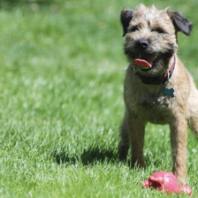
\includegraphics[width=0.25\textwidth, height=0.25\textwidth]{figure/segmentation_comparison/lime_rectangular-img0.png}};
    \node[SIR, label={[align=center]\textbf{\ac{lime} applied to}\\\textbf{rectangular regions}}] (id2) [right=of id1] {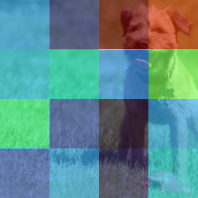
\includegraphics[width=0.25\textwidth, height=0.25\textwidth]{figure/segmentation_comparison/lime_rectangular-img1.png}};
    \node[SIR, label={[align=center]\textbf{\ac{lime} applied to}\\\textbf{superpixel regions}}] (id3) [right=of id2] {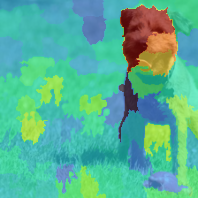
\includegraphics[width=0.25\textwidth, height=0.25\textwidth]{figure/segmentation_comparison/lime_slic-img1.png}};


    \end{tikzpicture}

    \end{center}
    \caption[Segmentation comparison]{Figure showing a comparison between running the \ac{lime} algorithm on rectangular and superpixel regions}
    \label{fig:segmentationcomp}
\end{figure}

Secondly, given that we have so many features, it may no longer be interesting to know exactly how much each feature contributes to a prediction, given that we don't expect any single pixel to have a very large impact. Instead we may be interested in how important pixels are relative to each other, or we may not be interested singular pixels at all.



With these limitations in mind,

\subsection{Specific methods}


The following section goes through several specific \ac{xai} methods. This serves two purposes: Firstly, it aids the first objective mentioned in section \ref{section:problemstatement}, by explaining how commonly used \ac{xai} methods function in practice, and by elucidating exactly how one is able to go from gradients, counterfactuals and other model outputs to human interpretable explanations. Secondly, this section also covers the specific methods that will be analyzed and evaluated as part of the rest of the objectives. By thoroughly detailing the functions of these methods in this chapter, it becomes easier to analyse and explain the results in chapter \ref{chapter:experiments}
\\


\subsubsection{Local Interpretable Model-Agnostic Explanations (LIME)}

\ac{lime} \cite{lime} is built on the idea that while the decision function of a large neural network (or any other large model) might be far too complex to easily interpret, it can most likely be approximated quite well by a simpler function, as long as we only look at the feature space around a single data point. For example, we could approximate a large feed forward neural network with a simple linear regression model, which can be intrinsically explained due to its low complexity.

To create a locally interpretable model, we need a neighbourhood of data points around our point of interest. To do this, we can sample a number of points from our dataset and weigh them by their distance to our original point. This sampling can be done in many ways, for example by calculating a mean and variance for each feature and sampling from a normal distribution. For image data, we can create new points similar to the image by masking out different regions of the image \cite{molnar}. The distance measure depends on the type of data we are dealing with. Regardless, the distance values are passed through a smoothing kernel which can be tuned to adjust the size of the "neighbourhood".

With these new data points, we can generate new predictions using the original, complex model. Thus, we now have a series of points, each with a weighting based on their distance to our original point, and each with a predicted score from our original model. With such a dataset, we can train a simpler model, which will then approximate the complex model around the point of interest. By inspecting this simple model (for example the learned weights of a linear regression model, or the structure of a decision tree), we can learn approximately how the complex model functions in a region around this single data point.

\subsubsection{Class Activation Mapping (CAM)}

\ac{cam} \cite{cam} is a model dependent, post hoc \ac{xai} method, which is used on Convolutional Neural Nets (\ac{cnn}s). For a specific output node of a model (for example, the one denoting the presence of a specific class, such as "cat"), \ac{cam} outputs a heat map showing which areas of the input image contributed to this node. In this way, \ac{cam} gives a visual explanation to which parts of an image the model focused on when making a decision to classify an image to a specific class. This method is model dependent, because it requires a specific architecture in the final layers of the network to work.

\ac{cam} is a relatively simple method to understand. It exploits the fact that various convolutional layers of \ac{cnn}s actually behave as object detectors, even when the training objective is classification \cite{cam}. As \cite{lenet5} explains, the earlier layers "extract elementary visual features such as oriented edges, end-points [or] corners", which can be used by subsequent layers to detect higher-order features. In this manner, the final convolutional layer will detect very high level visual features, combining the extracted information from all the previous layers. This layer is composed of several feature maps, where each map can be thought of as denoting the presence of some specific feature across the original image. The authors perform global average pooling (GAP) on these feature maps, giving a single value for each map, which is followed by a single dense layer and the Softmax activation function. In this way, each output node in the final layer is a weighted sum of all the global average pooled feature maps from the final convolutional layer. This means that we can represent the areas of the image which were used to perform the classification by performing the same weighted sum on the actual feature maps instead, which gives us a heat map which we can overlay on the original image (after upsampling the feature maps).

Figure \ref{camimg} shows the process visually. From this we can see that the resulting Class Activation Map (bottom right) gives an intuitive explanation for why the image in the top left gives a high score for the presence of the class "Australian Terrier".

\begin{figure}[h]
\centerline{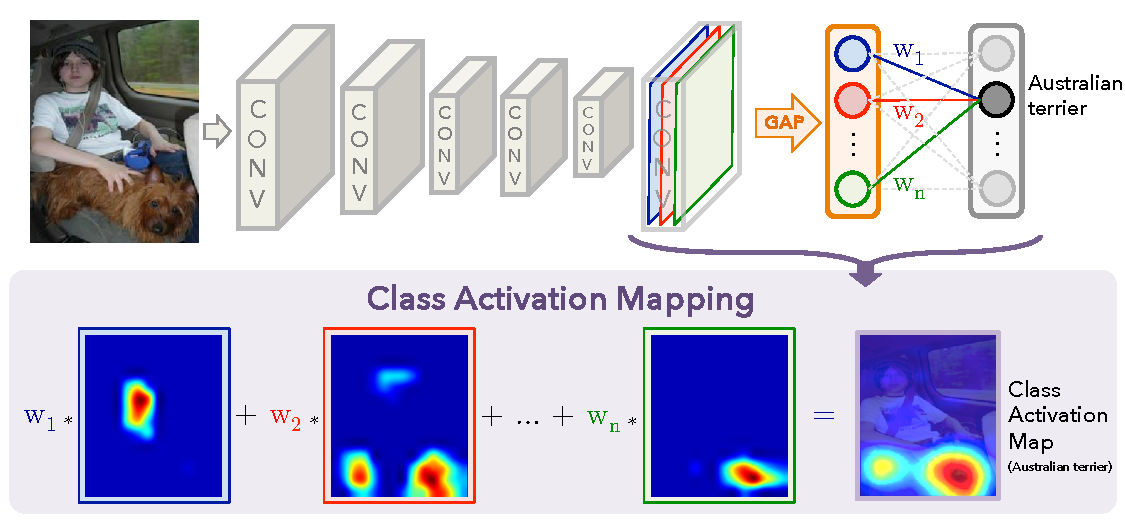
\includegraphics[width=3.25in]{figure/cam.pdf}}
\caption{Figure taken from \cite{cam}, showing the steps required to create a Class Activation Map}
\label{camimg}
\end{figure}

\begin{figure}[H]
    \begin{center}
    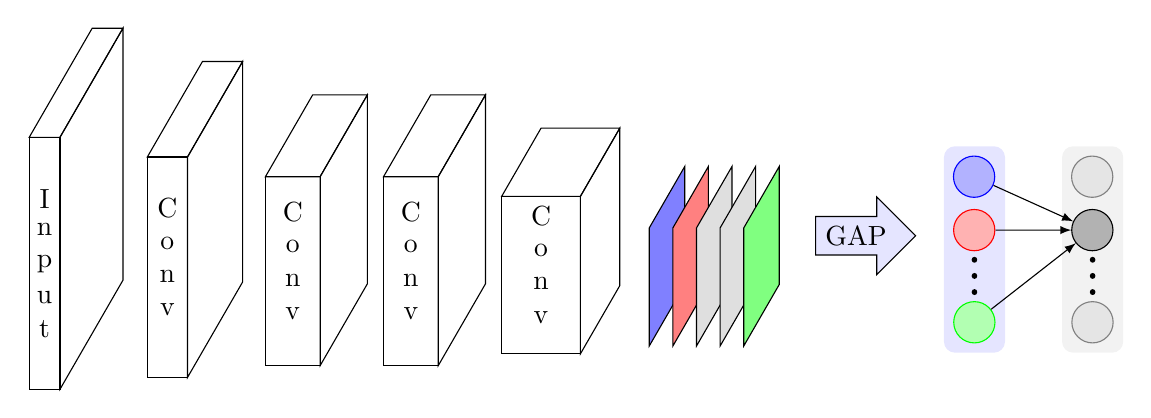
\begin{tikzpicture}[x={(1,0)},y={(0,1)},z={({cos(60)},{sin(60)})}, scale=1.5]
%
% comment these out if you want to see where the axes point to
% \draw[-latex] (0,0,0) -- (3,0,0) node[below]{$x$};
% \draw[-latex] (0,0,0) -- (0,3,0) node[left]{$y$};
% \draw[-latex] (0,0,0) -- (0,0,3) node[below]{$z$};
% a plane
\draw pic (box1-1) at (1,-1.6/2,0) {fake box=white!70!gray with dimensions {1/1.6/1.6} and {2*1.6} and {1*1.6} and Input};

\foreach \X [count=\Y] in {1.4,1.2,1.2,1}
{
    \draw pic (box1-\Y) at (\Y+1,-\X/2,0) {fake box=white!70!gray with dimensions {1/\X/\X} and {2*\X} and {1*\X} and Conv};
}

\foreach \X/\Col in {6.5/blue,6.7/red,6.9/lightgray, 7.1/lightgray, 7.3/green}
{\draw[canvas is yz plane at x = \X, transform shape, fill =
\Col!50!white] (0,0.10) rectangle (1,-0.5);}
% \draw[gray!60,thick] (6.3,-0.1,-1.6) coordinate (1-1) -- (6.3,-0.1,0.6) coordinate (1-2) -- (6.3,2.,0.6) coordinate (1-3) -- (6.3,2.1,-1.6) coordinate (1-4) -- cycle;
% \draw[gray!60,thick] (7.1,-0.1,-1.6) coordinate (2-1) -- (7.1,-0.1,0.6) coordinate (2-2) -- (7.1,2.,0.6) coordinate (2-3) -- (7.1,2.1,-1.6) coordinate (2-4) -- cycle;
% \foreach \X in {4,1,3}
% {\draw[gray!60,thick] (1-\X) -- (2-\X);}
%
\node[draw,single arrow, fill=blue!10] at (8,0.5,0) {GAP};
\node[circle,draw,blue,fill=blue!30] (A1) at (9,1,0) {~~~};
\node[circle,draw,red,fill=red!30,below=4pt of A1] (A2) {~~~};
\node[circle,draw,green,fill=green!30,below=18pt of A2] (A3) {~~~};
\draw[circle dotted, line width=2pt,shorten <=3pt] (A2) -- (A3);
\node[circle,draw,gray,fill=gray!20] (B1) at (10,1,0) {~~~};
\node[circle,draw,fill=gray!60,below=4pt of B1] (B2) {~~~};
\node[circle,draw,gray,fill=gray!20,below=18pt of B2] (B3) {~~~};
\draw[circle dotted, line width=2pt,shorten <=3pt] (B2) -- (B3);
\begin{scope}[on background layer]
\node[orange,thick,rounded corners,fill=blue!10,fit=(A1) (A3)]{};
\node[gray,thick,rounded corners,fill=gray!10,fit=(B1) (B3)]{};
\end{scope}
\foreach \X in {1,2,3}
{\draw[-latex] (A\X) -- (B2);}
\end{tikzpicture}

    \end{center}
    \caption[CNN example]{Figure showing a high level overview of how a CNN functions}
    \label{fig:cam2}
\end{figure}

Although \ac{cam} is an intuitive and effective method of visualizing the inner workings of a \ac{cnn}, it has some downsides. Firstly, it is highly model dependent, requiring that the model only have a single dense layer after the convolutions. Although there are some state of the art models which only use a single dense layer, this still places a limit on what models can be used, or requires the simplification of models that use more than a single dense layer. \cite[4]{cam} notes a 1-2\% drop in classification performance when performing this simplification. Secondly, the output of \ac{cam} is simply a weighted sum of all the feature maps after the final convolutional layer. As we move deeper in a \ac{cnn}, we reduce the spatial resolution by downsampling, while increasing the number of channels (increasing the depth of the output while reducing the height and width). Because of this, the \ac{cam} will have a drastically lower resolution than the original image, often less than $10 \, x \, 10$, while the input image may be hundreds of pixels in both dimensions. Because of this, \ac{cam} can only show general areas, as opposed to pixel wise explanations.
\\

\subsubsection{Gradient Class Activation Mapping (GradCAM)} \label{section:gradcam}

\ac{gradcam} \cite{gradcam} is an improvement on \ac{cam}, which generalizes the method to function with any \ac{cnn} architecture, thus making the method much less model dependent and avoiding the performance drop incurred when simplifying the model with \ac{cam}. Instead of using the weights of a final layer to calculate a weighted sum of feature maps in the last convolutional layer, \ac{gradcam} uses gradients flowing from the relevant output node to the activation maps to calculate the weights for each feature map. Furthermore, the authors prove that this method is a strict generalization of \ac{cam} \cite[5]{gradcam}, so that no information is lost by using gradients instead of weights.

Like the simplicity of the \ac{cam} method, the calculation of the weights using the gradients is also quite simple, as seen in Equation \ref{gradcameq}.

\begin{equation}
\alpha^c_k = \frac{1}{Z} \sum_i \sum_j \frac{\delta y^c}{\delta A^k_{ij}}
\label{gradcameq}
\end{equation}

Here, $c$ represents the index of the class we are interested in, $k$ the index of the feature map, and $i$ and $j$ the width and height of the image. $y^c$ is the element of the output vector $y$ which corresponds to the class $c$, while $A^k$ is the $k$'th feature map. $Z$ is equal to $i * j$, and simply normalizes the sum. Thus, we are actually just performing global average pooling of the gradients of $A^k$ with respect to $y^c$, which gives us a single value we can use as the weight for this feature map. Doing this for all feature maps for a specific class gives us all the weights we need to calculate a weighted sum, which we can upsample and visualize to get an explanation for the decision of the \ac{cnn}.

Thus, \ac{gradcam} improves upon \ac{cam} by making the method less model dependent. However, the explanations are still the same low resolution, which may not be ideal in all cases.
\\

\subsubsection{Guided Backpropagation}

Guided backpropagation is another \ac{xai} method which utilizes the gradients of the network with regards to the input to generate an explanation.

% \subsubsection{Layer-Wise Relevance Propagation (LRP)}
%
% LRP is another \ac{xai} method which generates a visual explanation of the areas of an image which lead to a classification decision. Unlike \ac{cam} and \ac{gradcam} LRP outputs a map which describes the relevance of every single pixel in the input image, and is thus produces a much more fine grained explanation than these other methods. LRP also differs in that \cite{lrp} does not define it as a specific method, but rather as a concept defined by a certain set of constraints which can be satisfied by different implementations depending on the type of model.
%
% LRP assumes that we can model the relevance $R_i$ for any node $i$ in a neural network, and aims to find the relevance for all the input nodes (the pixels in an image). Relevance is the contribution of any node to the final prediction $f(x)$ of a network, and the idea is to take the relevance of the output layer (simply defined as the output $f(x)$), and iteratively propagate this backwards through the network. Relevance scores are subject to a conservation property, which means that the sum of relevances must be equal for all layers (Equation \ref{lrpeq}). Furthermore, nodes must also conserve relevance, such that the sum of relevances a node receives from the previous layer is equal to the amount it distributes to the next layer. Once the relevance scores have been propagated from the output to the input layer in accordance with these constraints, we have a measure for how each input pixel contributed to the final output.
%
% \begin{equation}
% f(x) = ... = \sum_{d \in l + 1} R^{(l + 1)}_d = \sum_{d \in l + 1} R^{(l + 1)}_d = ... = \sum_d R^{(1)}_d
% \label{lrpeq}
% \end{equation}
%
% To distribute relevance between the nodes in a way which obeys the constraints defined in Equation \ref{lrpeq}, a rule for propagation of relevances must be defined. As \cite{lrp} shows, simply satisfying the constraints is not guaranteed to lead to meaningful explanations, nor is the decomposition of relevance unique. However, they show that by using a suitable propagation rule, we gain a visual explanation which shows which areas contribute to the final decision and which areas make the final decision less likely \cite[28]{lrp}.
% \\


\subsubsection{Occlusion methods}

Occlusion methods are a family of post-hoc model independent \ac{xai} methods. They function by masking different parts of the image and inspecting the change in output score. If an area leads to a large drop in softmax score for the predicted class when masked, this area must have been important for the network when making the prediction. The mask can be as simple as replacing all masked pixels with a single color, such as gray \cite{occlusion}, or they could use more advanced inpainting methods using generative models, for example by replacing a masked tumor with generated healthy tissue. 

Regardless of the mask, one can easily calculate the importance of any pixel for a prediction by calculating the average change in the output score for all masks which contain the specific pixel \cite{diagnostic}. Occlusion methods have the advantage of being completely model independent, since they do not consider the internals of the model. However, the computation can be expensive, because we need to run a forward pass for each position of the mask on the image. Figure \ref{fig:occlusion} shows the process visually.

% TODO: Make a picture



\section{Out-of-Distribution Detection} \label{ood_intro}

This section discusses \ac{ood} detection, the field which attempts to tackle the second problem discussed in the introduction; that \ac{ml} models have significantly worse performance on \ac{ood} data points and will often "fail silently", making completely wrong predictions with apparent high confidence \cite{adversarial}. \ac{ood} detection is a developing field, and still in an initial stage \cite{ooddl}. In 2017, \cite{oodbaseline} proposed a baseline \ac{ood} detection method. This section will discuss this method and the methods which follow it.

\subsection{Motivation for Out-of-Distribution Detection}

When training a model using supervised learning, we implicitly use the "closed-world assumption", which means that we assume that test data will be drawn from the same distribution as the training data \cite{oodoverview}. However, when a model is deployed, the data we see may not obey this assumption. Without \ac{ood} detection, the model will behave in the exact same way when encountering \ac{ood} samples or in distribution (ID) samples, and may even claim to be highly confident in its prediction although the sample is far away from the distribution of the training data \cite[1]{energy}. In any system where models make high impact decisions, this is a huge problem. We do not want a model to claim high confidence when predicting if a woman has lung cancer if the model has only been trained on men, nor do we want a model to attempt to classify a rare disease that was not part of the training data. Thus, \ac{ood} detection methods are necessary, so that \ac{ood} samples can be caught before the model makes a prediction and dealt with correctly.

Intuitively, one might assume that distinguishing ID and \ac{ood} samples from each other can be solved by simple binary classification using a dataset of ID samples and one of \ac{ood} samples. Indeed, if one has sufficient amount of high quality \ac{ood} samples, this can be done. However, this can be difficult to obtain in practice \cite[15]{oodoverview}, thus requiring more sophisticated methods of \ac{ood} detection.

\subsection{Semantic versus covariate shift}

The first distinction to make in \ac{ood} detection tasks is whether an \ac{ood} sample is \ac{ood} because of {\it semantic} or {\it covariate} shift. Semantic shift refers to samples with different classes than the ones the model is trained on. A picture of a giraffe would represent a semantic shift for a model trained to differentiate between different breeds of dogs, as a giraffe does not belong to any breed of dog. Covariate shift refers to samples which come from a different distribution while still belonging to one of the classes of the original data set. An image of a Beagle puppy could represent covariate shift for a dog breed classifier despite Beagle being one of the classes, if all ID images were of adult dogs. Likewise, an image of a dog in a dark room could represent covariate shift, if all the ID images were of dogs outside, in well lit conditions. Figure \ref{fig:semanticcovariate} shows this distinction visually. Here, we can easily see the difference between covariate and semantic shift; covariate shifted images come from the same classes as \ac{id} samples, while semantically shifted images come from completely unknown classes.

\begin{figure}[H]
    \begin{center}

    \begin{tikzpicture}[
    SIR/.style={rectangle, draw=black!60, thick, minimum size=5mm},
    ]

    \node[SIR, label={[align=center, above=0.2cm]\textbf{In Distribution}\\\textbf{images}}] (id1) {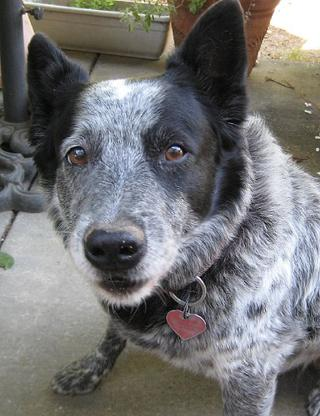
\includegraphics[width=0.25\textwidth, height=0.25\textwidth]{figure/semanticcovariate/id1.jpg}};
    \node[SIR] (id2) [below=of id1] {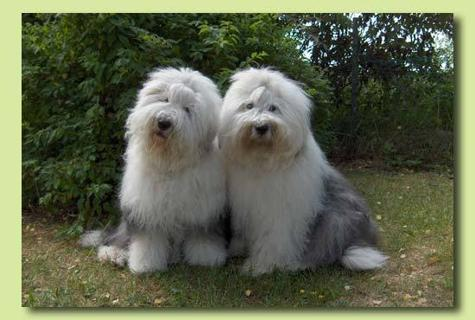
\includegraphics[width=0.25\textwidth, height=0.25\textwidth]{figure/semanticcovariate/id2.jpg}};
    \node[SIR] (id3) [below=of id2] {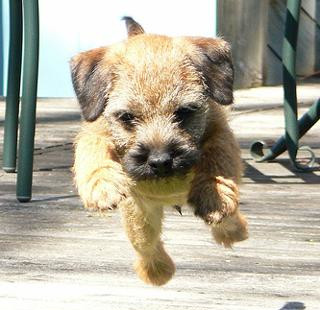
\includegraphics[width=0.25\textwidth, height=0.25\textwidth]{figure/semanticcovariate/id3.jpg}};

    \node[SIR, label={[align=center, above=0.2cm]\textbf{Covariate shifted}\\\textbf{images}}, right=of id1] (cov1) {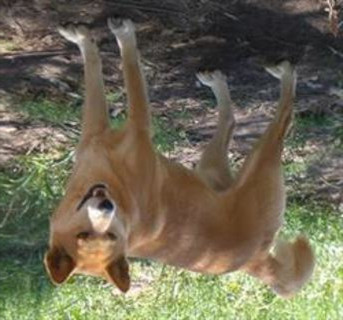
\includegraphics[width=0.25\textwidth, height=0.25\textwidth]{figure/semanticcovariate/cov1.jpg}};
    \node[SIR] (cov2) [below=of cov1] {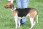
\includegraphics[width=0.25\textwidth, height=0.25\textwidth]{figure/semanticcovariate/cov2.jpg}};
    \node[SIR] (cov3) [below=of cov2] {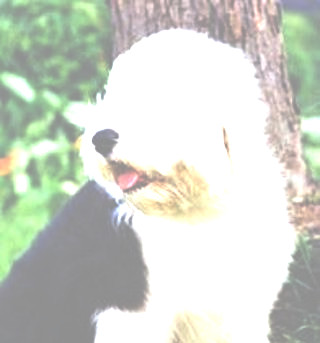
\includegraphics[width=0.25\textwidth, height=0.25\textwidth]{figure/semanticcovariate/cov3.jpg}};

    \node[SIR, label={[align=center, above=0.2cm]\textbf{Semantically shifted}\\\textbf{images}}, right=of cov1] (sem1) {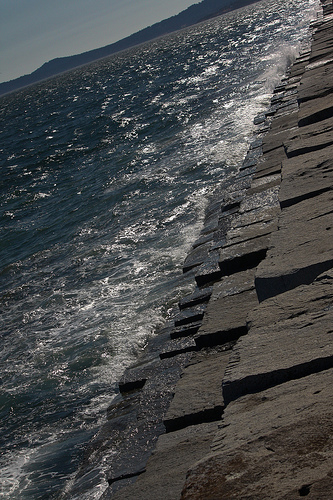
\includegraphics[width=0.25\textwidth, height=0.25\textwidth]{figure/semanticcovariate/sem1.jpg}};
    \node[SIR] (sem2) [below=of sem1] {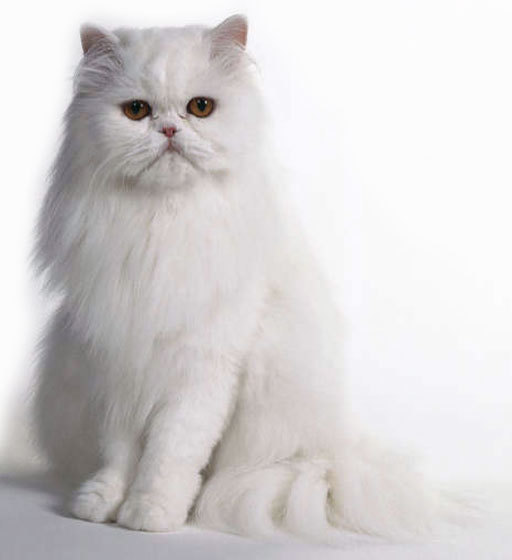
\includegraphics[width=0.25\textwidth, height=0.25\textwidth]{figure/semanticcovariate/sem2.jpg}};
    \node[SIR] (sem3) [below=of sem2] {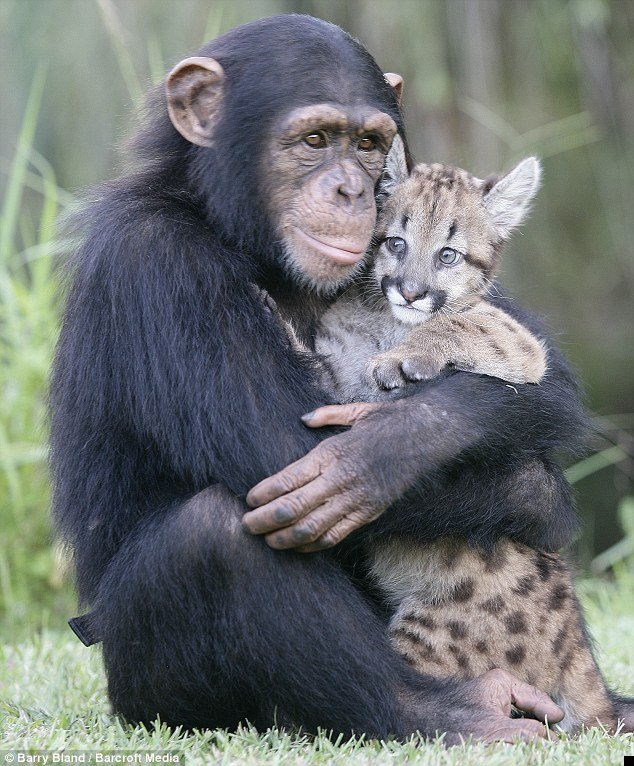
\includegraphics[width=0.25\textwidth, height=0.25\textwidth]{figure/semanticcovariate/sem3.jpg}};

    \begin{scope}[on background layer={color=id!50}]
        \fill (-2.5,2.15) rectangle (2.5,-12.1);
    \end{scope}

    \begin{scope}[on background layer={color=near!50}]
        \fill (2.5,2.15) rectangle (7.5,-12.1);
    \end{scope}

    \begin{scope}[on background layer={color=far!50}]
        \fill (7.5,2.15) rectangle (12.5,-12.1);
    \end{scope}

    \end{tikzpicture}

    \caption[Mean Saliency visual explanation]{Figure showing in-distribution, covariate shifted and semantically shifted images for an imagined dog breed classifier. Images are taken from the ImageNet dataset}
    \label{fig:semanticcovariate}

    \end{center}
\end{figure}

The detection of semantic shift, as opposed to covariate shift, is the main focus of most \ac{ood} detection tasks \cite{oodoverview}. In many applications, it is expected that the model should be able to generalize its prediction to covariate-shifted data, and therefore the focus is on detecting semantic shift. However, the field of medical image classification is one where detecting covariate shift is also important, as the model should only make predictions on data points which are very similar to its training data \cite{oodoverview}.

Given that the detection of semantic shift has been the main focus of most \ac{ood} literature, my work will primarily deal with semantic shift as well. Thus, unless otherwise specified, when I refer to \ac{ood} data points, I mean data points which are semantically shifted, i.e that come from another class than those the model has been trained on.

\subsection{Benchmarking}

The performance of an \ac{xai} is hard to quantify, because the quality of an explanation is not easily reduced to a number. For \ac{ood} detection, performance is much easier to measure, as the problem can be described as a binary classification problem, with \ac{ood} and ID samples as the positive and negative class. Thus, we can calculate many different metrics and compare methods against each other. For \ac{ood} methods, the two most common metrics to report are \ac{fpr95} and the \ac{auroc} (see section \ref{section:aurocfpr95}). It is common to use ImageNet or CIFAR as the ID dataset, and calculate FPR95 and AUROC on other datasets which contain no overlapping class labels. When selecting \ac{ood} datasets, it is common to differentiate between \textbf{near-\ac{ood}} and \textbf{far-\ac{ood}}. Far-\ac{ood} samples are samples which are drastically different from the ID samples, while near-\ac{ood} samples only differ slightly. For our cat-versus-dog classifier, a tiger and a wolf would represent near-\ac{ood} semantic shift, while a plane and a car would represent far-\ac{ood} semantic shift. As one might expect, detecting near-\ac{ood} samples is much harder.

% FPR95 is, as the name implies, the number of false positives (i.e the number of ID data points that the method falsely believes to be \ac{ood}) when 95\% of the \ac{ood} data points are correctly detected. AUROC can defined as the chance that a random ID data point has a higher ID-score than a random \ac{ood} data point \cite{openood}. An AUROC of 0.5 is equivalent to random guessing, while an AUROC of 1 is a perfect model that catches all \ac{ood} data points.


In 2021, \cite{oodoverview} defined a generalized \ac{ood} detection framework, and in 2023 \cite{openood} introduced a comprehensive benchmark of all relevant \ac{ood} methods under this framework, which allows for accurate comparisons of methods within the field. This benchmark is discussed in detail in section \ref{chapter:openood}.

\subsection{Methods}

This section will follow the same outline as section \ref{chapter:xai}; firstly, the overarching categories of methods will be discussed, followed by a more detailed look at a selection of specific methods within the field.
\\

The field of \ac{ood} is separated into four categories of methods \cite{oodoverview}:

\begin{itemize}
  \item Classification-based methods
  \item Density-based methods
  \item Distance-based methods
  \item Reconstruction-based methods
\end{itemize}

All methods can also be categorized by whether they are post-hoc or training based. Post-hoc methods take an already trained network and attempt to extract information which separates ID and \ac{ood} samples out of the network during inference. These methods have the obvious advantage that they can work out of the box with large pre-trained network without requiring expensive training from scratch. Training based methods train the network in ways which maximize the difference between ID and \ac{ood} samples. These methods do not necessarily require \ac{ood} samples, but can train using auxiliary loss functions which amplify the differences in network behaviour when faced with \ac{ood} data as opposed to ID. Regardless, these methods come with a much higher computational requirement than post-hoc methods, as they require training from scratch or at least retraining using the new loss criterion. 

Given the fact that post-hoc methods can be applied to trained networks out of the box, it is quite common to combine both post-hoc and training strategies to achieve the best performance.


Below follows a short explanation of each the four categories mentioned above.
\\

\subsubsection{Classification-based methods}

Classification-based methods usually use the softmax score or logits of a model to attempt to distinguish \ac{ood} and ID samples. \cite{oodbaseline} made the observation that while the softmax score may be a poor indication of the actual confidence of the model on a single data point, it is still higher on average for ID samples as opposed to \ac{ood} samples. By using this simple distinction, they created a baseline model which separated \ac{ood} and ID samples. Using input perturbations and temperature scaling, \cite{odin} further improved on this method, by amplifying the difference in softmax score of ID and \ac{ood} data. 

More generally, classification-based methods do not need to use the softmax score, but may attempt to find any metric which separates the distribution of ID samples from \ac{ood} samples. Figure \ref{fig:ood_metric} shows the probability density for an unspecified metric for both \ac{ood} and ID samples. The goal of classification-based \ac{ood} detection is to find metrics or training methods which make these probability densities have as little overlap as possible, such that they are easily separated by a threshold.

There are several state of the art methods which utilize a classification-based approach, and these make up a large part of the representative methodologies for \ac{ood} detection today \cite[8]{oodoverview}. As such, I shall devote the majority of section \ref{ood_specific} to classification-based methods.

\begin{figure}
    \label{fig:ood_metric}
    \begin{center}
        %% Creator: Matplotlib, PGF backend
%%
%% To include the figure in your LaTeX document, write
%%   \input{<filename>.pgf}
%%
%% Make sure the required packages are loaded in your preamble
%%   \usepackage{pgf}
%%
%% Also ensure that all the required font packages are loaded; for instance,
%% the lmodern package is sometimes necessary when using math font.
%%   \usepackage{lmodern}
%%
%% Figures using additional raster images can only be included by \input if
%% they are in the same directory as the main LaTeX file. For loading figures
%% from other directories you can use the `import` package
%%   \usepackage{import}
%%
%% and then include the figures with
%%   \import{<path to file>}{<filename>.pgf}
%%
%% Matplotlib used the following preamble
%%   \def\mathdefault#1{#1}
%%   \everymath=\expandafter{\the\everymath\displaystyle}
%%   \IfFileExists{scrextend.sty}{
%%     \usepackage[fontsize=10.000000pt]{scrextend}
%%   }{
%%     \renewcommand{\normalsize}{\fontsize{10.000000}{12.000000}\selectfont}
%%     \normalsize
%%   }
%%   
%%   \makeatletter\@ifpackageloaded{underscore}{}{\usepackage[strings]{underscore}}\makeatother
%%
\begingroup%
\makeatletter%
\begin{pgfpicture}%
\pgfpathrectangle{\pgfpointorigin}{\pgfqpoint{6.400000in}{4.800000in}}%
\pgfusepath{use as bounding box, clip}%
\begin{pgfscope}%
\pgfsetbuttcap%
\pgfsetmiterjoin%
\definecolor{currentfill}{rgb}{1.000000,1.000000,1.000000}%
\pgfsetfillcolor{currentfill}%
\pgfsetlinewidth{0.000000pt}%
\definecolor{currentstroke}{rgb}{1.000000,1.000000,1.000000}%
\pgfsetstrokecolor{currentstroke}%
\pgfsetdash{}{0pt}%
\pgfpathmoveto{\pgfqpoint{0.000000in}{0.000000in}}%
\pgfpathlineto{\pgfqpoint{6.400000in}{0.000000in}}%
\pgfpathlineto{\pgfqpoint{6.400000in}{4.800000in}}%
\pgfpathlineto{\pgfqpoint{0.000000in}{4.800000in}}%
\pgfpathlineto{\pgfqpoint{0.000000in}{0.000000in}}%
\pgfpathclose%
\pgfusepath{fill}%
\end{pgfscope}%
\begin{pgfscope}%
\pgfsetbuttcap%
\pgfsetmiterjoin%
\definecolor{currentfill}{rgb}{1.000000,1.000000,1.000000}%
\pgfsetfillcolor{currentfill}%
\pgfsetlinewidth{0.000000pt}%
\definecolor{currentstroke}{rgb}{0.000000,0.000000,0.000000}%
\pgfsetstrokecolor{currentstroke}%
\pgfsetstrokeopacity{0.000000}%
\pgfsetdash{}{0pt}%
\pgfpathmoveto{\pgfqpoint{0.800000in}{0.528000in}}%
\pgfpathlineto{\pgfqpoint{5.760000in}{0.528000in}}%
\pgfpathlineto{\pgfqpoint{5.760000in}{4.224000in}}%
\pgfpathlineto{\pgfqpoint{0.800000in}{4.224000in}}%
\pgfpathlineto{\pgfqpoint{0.800000in}{0.528000in}}%
\pgfpathclose%
\pgfusepath{fill}%
\end{pgfscope}%
\begin{pgfscope}%
\pgfpathrectangle{\pgfqpoint{0.800000in}{0.528000in}}{\pgfqpoint{4.960000in}{3.696000in}}%
\pgfusepath{clip}%
\pgfsetbuttcap%
\pgfsetroundjoin%
\definecolor{currentfill}{rgb}{0.501961,0.501961,0.501961}%
\pgfsetfillcolor{currentfill}%
\pgfsetfillopacity{0.500000}%
\pgfsetlinewidth{1.003750pt}%
\definecolor{currentstroke}{rgb}{0.501961,0.501961,0.501961}%
\pgfsetstrokecolor{currentstroke}%
\pgfsetstrokeopacity{0.500000}%
\pgfsetdash{}{0pt}%
\pgfsys@defobject{currentmarker}{\pgfqpoint{1.025455in}{0.696000in}}{\pgfqpoint{5.534545in}{1.722527in}}{%
\pgfpathmoveto{\pgfqpoint{1.025455in}{0.696000in}}%
\pgfpathlineto{\pgfqpoint{1.025455in}{0.696000in}}%
\pgfpathlineto{\pgfqpoint{1.029968in}{0.696000in}}%
\pgfpathlineto{\pgfqpoint{1.034482in}{0.696000in}}%
\pgfpathlineto{\pgfqpoint{1.038995in}{0.696000in}}%
\pgfpathlineto{\pgfqpoint{1.043509in}{0.696000in}}%
\pgfpathlineto{\pgfqpoint{1.048023in}{0.696000in}}%
\pgfpathlineto{\pgfqpoint{1.052536in}{0.696000in}}%
\pgfpathlineto{\pgfqpoint{1.057050in}{0.696000in}}%
\pgfpathlineto{\pgfqpoint{1.061563in}{0.696000in}}%
\pgfpathlineto{\pgfqpoint{1.066077in}{0.696000in}}%
\pgfpathlineto{\pgfqpoint{1.070591in}{0.696000in}}%
\pgfpathlineto{\pgfqpoint{1.075104in}{0.696000in}}%
\pgfpathlineto{\pgfqpoint{1.079618in}{0.696000in}}%
\pgfpathlineto{\pgfqpoint{1.084131in}{0.696000in}}%
\pgfpathlineto{\pgfqpoint{1.088645in}{0.696000in}}%
\pgfpathlineto{\pgfqpoint{1.093159in}{0.696000in}}%
\pgfpathlineto{\pgfqpoint{1.097672in}{0.696000in}}%
\pgfpathlineto{\pgfqpoint{1.102186in}{0.696000in}}%
\pgfpathlineto{\pgfqpoint{1.106699in}{0.696000in}}%
\pgfpathlineto{\pgfqpoint{1.111213in}{0.696000in}}%
\pgfpathlineto{\pgfqpoint{1.115727in}{0.696000in}}%
\pgfpathlineto{\pgfqpoint{1.120240in}{0.696000in}}%
\pgfpathlineto{\pgfqpoint{1.124754in}{0.696000in}}%
\pgfpathlineto{\pgfqpoint{1.129267in}{0.696000in}}%
\pgfpathlineto{\pgfqpoint{1.133781in}{0.696000in}}%
\pgfpathlineto{\pgfqpoint{1.138295in}{0.696000in}}%
\pgfpathlineto{\pgfqpoint{1.142808in}{0.696000in}}%
\pgfpathlineto{\pgfqpoint{1.147322in}{0.696000in}}%
\pgfpathlineto{\pgfqpoint{1.151835in}{0.696000in}}%
\pgfpathlineto{\pgfqpoint{1.156349in}{0.696000in}}%
\pgfpathlineto{\pgfqpoint{1.160863in}{0.696000in}}%
\pgfpathlineto{\pgfqpoint{1.165376in}{0.696000in}}%
\pgfpathlineto{\pgfqpoint{1.169890in}{0.696000in}}%
\pgfpathlineto{\pgfqpoint{1.174403in}{0.696000in}}%
\pgfpathlineto{\pgfqpoint{1.178917in}{0.696000in}}%
\pgfpathlineto{\pgfqpoint{1.183431in}{0.696000in}}%
\pgfpathlineto{\pgfqpoint{1.187944in}{0.696000in}}%
\pgfpathlineto{\pgfqpoint{1.192458in}{0.696000in}}%
\pgfpathlineto{\pgfqpoint{1.196972in}{0.696000in}}%
\pgfpathlineto{\pgfqpoint{1.201485in}{0.696000in}}%
\pgfpathlineto{\pgfqpoint{1.205999in}{0.696000in}}%
\pgfpathlineto{\pgfqpoint{1.210512in}{0.696000in}}%
\pgfpathlineto{\pgfqpoint{1.215026in}{0.696000in}}%
\pgfpathlineto{\pgfqpoint{1.219540in}{0.696000in}}%
\pgfpathlineto{\pgfqpoint{1.224053in}{0.696000in}}%
\pgfpathlineto{\pgfqpoint{1.228567in}{0.696000in}}%
\pgfpathlineto{\pgfqpoint{1.233080in}{0.696000in}}%
\pgfpathlineto{\pgfqpoint{1.237594in}{0.696000in}}%
\pgfpathlineto{\pgfqpoint{1.242108in}{0.696000in}}%
\pgfpathlineto{\pgfqpoint{1.246621in}{0.696000in}}%
\pgfpathlineto{\pgfqpoint{1.251135in}{0.696000in}}%
\pgfpathlineto{\pgfqpoint{1.255648in}{0.696000in}}%
\pgfpathlineto{\pgfqpoint{1.260162in}{0.696000in}}%
\pgfpathlineto{\pgfqpoint{1.264676in}{0.696000in}}%
\pgfpathlineto{\pgfqpoint{1.269189in}{0.696000in}}%
\pgfpathlineto{\pgfqpoint{1.273703in}{0.696000in}}%
\pgfpathlineto{\pgfqpoint{1.278216in}{0.696000in}}%
\pgfpathlineto{\pgfqpoint{1.282730in}{0.696000in}}%
\pgfpathlineto{\pgfqpoint{1.287244in}{0.696000in}}%
\pgfpathlineto{\pgfqpoint{1.291757in}{0.696000in}}%
\pgfpathlineto{\pgfqpoint{1.296271in}{0.696000in}}%
\pgfpathlineto{\pgfqpoint{1.300784in}{0.696000in}}%
\pgfpathlineto{\pgfqpoint{1.305298in}{0.696000in}}%
\pgfpathlineto{\pgfqpoint{1.309812in}{0.696000in}}%
\pgfpathlineto{\pgfqpoint{1.314325in}{0.696000in}}%
\pgfpathlineto{\pgfqpoint{1.318839in}{0.696000in}}%
\pgfpathlineto{\pgfqpoint{1.323352in}{0.696000in}}%
\pgfpathlineto{\pgfqpoint{1.327866in}{0.696000in}}%
\pgfpathlineto{\pgfqpoint{1.332380in}{0.696000in}}%
\pgfpathlineto{\pgfqpoint{1.336893in}{0.696000in}}%
\pgfpathlineto{\pgfqpoint{1.341407in}{0.696000in}}%
\pgfpathlineto{\pgfqpoint{1.345920in}{0.696000in}}%
\pgfpathlineto{\pgfqpoint{1.350434in}{0.696000in}}%
\pgfpathlineto{\pgfqpoint{1.354948in}{0.696000in}}%
\pgfpathlineto{\pgfqpoint{1.359461in}{0.696000in}}%
\pgfpathlineto{\pgfqpoint{1.363975in}{0.696000in}}%
\pgfpathlineto{\pgfqpoint{1.368488in}{0.696000in}}%
\pgfpathlineto{\pgfqpoint{1.373002in}{0.696000in}}%
\pgfpathlineto{\pgfqpoint{1.377516in}{0.696000in}}%
\pgfpathlineto{\pgfqpoint{1.382029in}{0.696000in}}%
\pgfpathlineto{\pgfqpoint{1.386543in}{0.696000in}}%
\pgfpathlineto{\pgfqpoint{1.391057in}{0.696000in}}%
\pgfpathlineto{\pgfqpoint{1.395570in}{0.696000in}}%
\pgfpathlineto{\pgfqpoint{1.400084in}{0.696000in}}%
\pgfpathlineto{\pgfqpoint{1.404597in}{0.696000in}}%
\pgfpathlineto{\pgfqpoint{1.409111in}{0.696000in}}%
\pgfpathlineto{\pgfqpoint{1.413625in}{0.696000in}}%
\pgfpathlineto{\pgfqpoint{1.418138in}{0.696000in}}%
\pgfpathlineto{\pgfqpoint{1.422652in}{0.696000in}}%
\pgfpathlineto{\pgfqpoint{1.427165in}{0.696000in}}%
\pgfpathlineto{\pgfqpoint{1.431679in}{0.696000in}}%
\pgfpathlineto{\pgfqpoint{1.436193in}{0.696000in}}%
\pgfpathlineto{\pgfqpoint{1.440706in}{0.696000in}}%
\pgfpathlineto{\pgfqpoint{1.445220in}{0.696000in}}%
\pgfpathlineto{\pgfqpoint{1.449733in}{0.696000in}}%
\pgfpathlineto{\pgfqpoint{1.454247in}{0.696000in}}%
\pgfpathlineto{\pgfqpoint{1.458761in}{0.696000in}}%
\pgfpathlineto{\pgfqpoint{1.463274in}{0.696000in}}%
\pgfpathlineto{\pgfqpoint{1.467788in}{0.696000in}}%
\pgfpathlineto{\pgfqpoint{1.472301in}{0.696000in}}%
\pgfpathlineto{\pgfqpoint{1.476815in}{0.696000in}}%
\pgfpathlineto{\pgfqpoint{1.481329in}{0.696000in}}%
\pgfpathlineto{\pgfqpoint{1.485842in}{0.696000in}}%
\pgfpathlineto{\pgfqpoint{1.490356in}{0.696000in}}%
\pgfpathlineto{\pgfqpoint{1.494869in}{0.696000in}}%
\pgfpathlineto{\pgfqpoint{1.499383in}{0.696000in}}%
\pgfpathlineto{\pgfqpoint{1.503897in}{0.696000in}}%
\pgfpathlineto{\pgfqpoint{1.508410in}{0.696000in}}%
\pgfpathlineto{\pgfqpoint{1.512924in}{0.696000in}}%
\pgfpathlineto{\pgfqpoint{1.517437in}{0.696000in}}%
\pgfpathlineto{\pgfqpoint{1.521951in}{0.696000in}}%
\pgfpathlineto{\pgfqpoint{1.526465in}{0.696000in}}%
\pgfpathlineto{\pgfqpoint{1.530978in}{0.696000in}}%
\pgfpathlineto{\pgfqpoint{1.535492in}{0.696000in}}%
\pgfpathlineto{\pgfqpoint{1.540005in}{0.696000in}}%
\pgfpathlineto{\pgfqpoint{1.544519in}{0.696000in}}%
\pgfpathlineto{\pgfqpoint{1.549033in}{0.696000in}}%
\pgfpathlineto{\pgfqpoint{1.553546in}{0.696000in}}%
\pgfpathlineto{\pgfqpoint{1.558060in}{0.696000in}}%
\pgfpathlineto{\pgfqpoint{1.562573in}{0.696000in}}%
\pgfpathlineto{\pgfqpoint{1.567087in}{0.696000in}}%
\pgfpathlineto{\pgfqpoint{1.571601in}{0.696000in}}%
\pgfpathlineto{\pgfqpoint{1.576114in}{0.696000in}}%
\pgfpathlineto{\pgfqpoint{1.580628in}{0.696000in}}%
\pgfpathlineto{\pgfqpoint{1.585142in}{0.696000in}}%
\pgfpathlineto{\pgfqpoint{1.589655in}{0.696000in}}%
\pgfpathlineto{\pgfqpoint{1.594169in}{0.696000in}}%
\pgfpathlineto{\pgfqpoint{1.598682in}{0.696000in}}%
\pgfpathlineto{\pgfqpoint{1.603196in}{0.696000in}}%
\pgfpathlineto{\pgfqpoint{1.607710in}{0.696000in}}%
\pgfpathlineto{\pgfqpoint{1.612223in}{0.696000in}}%
\pgfpathlineto{\pgfqpoint{1.616737in}{0.696000in}}%
\pgfpathlineto{\pgfqpoint{1.621250in}{0.696000in}}%
\pgfpathlineto{\pgfqpoint{1.625764in}{0.696000in}}%
\pgfpathlineto{\pgfqpoint{1.630278in}{0.696000in}}%
\pgfpathlineto{\pgfqpoint{1.634791in}{0.696000in}}%
\pgfpathlineto{\pgfqpoint{1.639305in}{0.696000in}}%
\pgfpathlineto{\pgfqpoint{1.643818in}{0.696000in}}%
\pgfpathlineto{\pgfqpoint{1.648332in}{0.696000in}}%
\pgfpathlineto{\pgfqpoint{1.652846in}{0.696000in}}%
\pgfpathlineto{\pgfqpoint{1.657359in}{0.696000in}}%
\pgfpathlineto{\pgfqpoint{1.661873in}{0.696000in}}%
\pgfpathlineto{\pgfqpoint{1.666386in}{0.696000in}}%
\pgfpathlineto{\pgfqpoint{1.670900in}{0.696000in}}%
\pgfpathlineto{\pgfqpoint{1.675414in}{0.696000in}}%
\pgfpathlineto{\pgfqpoint{1.679927in}{0.696000in}}%
\pgfpathlineto{\pgfqpoint{1.684441in}{0.696000in}}%
\pgfpathlineto{\pgfqpoint{1.688954in}{0.696000in}}%
\pgfpathlineto{\pgfqpoint{1.693468in}{0.696000in}}%
\pgfpathlineto{\pgfqpoint{1.697982in}{0.696000in}}%
\pgfpathlineto{\pgfqpoint{1.702495in}{0.696000in}}%
\pgfpathlineto{\pgfqpoint{1.707009in}{0.696000in}}%
\pgfpathlineto{\pgfqpoint{1.711522in}{0.696000in}}%
\pgfpathlineto{\pgfqpoint{1.716036in}{0.696000in}}%
\pgfpathlineto{\pgfqpoint{1.720550in}{0.696000in}}%
\pgfpathlineto{\pgfqpoint{1.725063in}{0.696000in}}%
\pgfpathlineto{\pgfqpoint{1.729577in}{0.696000in}}%
\pgfpathlineto{\pgfqpoint{1.734090in}{0.696000in}}%
\pgfpathlineto{\pgfqpoint{1.738604in}{0.696000in}}%
\pgfpathlineto{\pgfqpoint{1.743118in}{0.696000in}}%
\pgfpathlineto{\pgfqpoint{1.747631in}{0.696000in}}%
\pgfpathlineto{\pgfqpoint{1.752145in}{0.696000in}}%
\pgfpathlineto{\pgfqpoint{1.756658in}{0.696000in}}%
\pgfpathlineto{\pgfqpoint{1.761172in}{0.696000in}}%
\pgfpathlineto{\pgfqpoint{1.765686in}{0.696000in}}%
\pgfpathlineto{\pgfqpoint{1.770199in}{0.696000in}}%
\pgfpathlineto{\pgfqpoint{1.774713in}{0.696000in}}%
\pgfpathlineto{\pgfqpoint{1.779226in}{0.696000in}}%
\pgfpathlineto{\pgfqpoint{1.783740in}{0.696000in}}%
\pgfpathlineto{\pgfqpoint{1.788254in}{0.696000in}}%
\pgfpathlineto{\pgfqpoint{1.792767in}{0.696000in}}%
\pgfpathlineto{\pgfqpoint{1.797281in}{0.696000in}}%
\pgfpathlineto{\pgfqpoint{1.801795in}{0.696000in}}%
\pgfpathlineto{\pgfqpoint{1.806308in}{0.696000in}}%
\pgfpathlineto{\pgfqpoint{1.810822in}{0.696000in}}%
\pgfpathlineto{\pgfqpoint{1.815335in}{0.696000in}}%
\pgfpathlineto{\pgfqpoint{1.819849in}{0.696000in}}%
\pgfpathlineto{\pgfqpoint{1.824363in}{0.696000in}}%
\pgfpathlineto{\pgfqpoint{1.828876in}{0.696000in}}%
\pgfpathlineto{\pgfqpoint{1.833390in}{0.696000in}}%
\pgfpathlineto{\pgfqpoint{1.837903in}{0.696000in}}%
\pgfpathlineto{\pgfqpoint{1.842417in}{0.696000in}}%
\pgfpathlineto{\pgfqpoint{1.846931in}{0.696000in}}%
\pgfpathlineto{\pgfqpoint{1.851444in}{0.696000in}}%
\pgfpathlineto{\pgfqpoint{1.855958in}{0.696000in}}%
\pgfpathlineto{\pgfqpoint{1.860471in}{0.696000in}}%
\pgfpathlineto{\pgfqpoint{1.864985in}{0.696000in}}%
\pgfpathlineto{\pgfqpoint{1.869499in}{0.696000in}}%
\pgfpathlineto{\pgfqpoint{1.874012in}{0.696000in}}%
\pgfpathlineto{\pgfqpoint{1.878526in}{0.696000in}}%
\pgfpathlineto{\pgfqpoint{1.883039in}{0.696000in}}%
\pgfpathlineto{\pgfqpoint{1.887553in}{0.696000in}}%
\pgfpathlineto{\pgfqpoint{1.892067in}{0.696000in}}%
\pgfpathlineto{\pgfqpoint{1.896580in}{0.696000in}}%
\pgfpathlineto{\pgfqpoint{1.901094in}{0.696000in}}%
\pgfpathlineto{\pgfqpoint{1.905607in}{0.696000in}}%
\pgfpathlineto{\pgfqpoint{1.910121in}{0.696000in}}%
\pgfpathlineto{\pgfqpoint{1.914635in}{0.696000in}}%
\pgfpathlineto{\pgfqpoint{1.919148in}{0.696000in}}%
\pgfpathlineto{\pgfqpoint{1.923662in}{0.696000in}}%
\pgfpathlineto{\pgfqpoint{1.928175in}{0.696000in}}%
\pgfpathlineto{\pgfqpoint{1.932689in}{0.696000in}}%
\pgfpathlineto{\pgfqpoint{1.937203in}{0.696000in}}%
\pgfpathlineto{\pgfqpoint{1.941716in}{0.696000in}}%
\pgfpathlineto{\pgfqpoint{1.946230in}{0.696000in}}%
\pgfpathlineto{\pgfqpoint{1.950743in}{0.696000in}}%
\pgfpathlineto{\pgfqpoint{1.955257in}{0.696000in}}%
\pgfpathlineto{\pgfqpoint{1.959771in}{0.696000in}}%
\pgfpathlineto{\pgfqpoint{1.964284in}{0.696000in}}%
\pgfpathlineto{\pgfqpoint{1.968798in}{0.696000in}}%
\pgfpathlineto{\pgfqpoint{1.973311in}{0.696000in}}%
\pgfpathlineto{\pgfqpoint{1.977825in}{0.696000in}}%
\pgfpathlineto{\pgfqpoint{1.982339in}{0.696000in}}%
\pgfpathlineto{\pgfqpoint{1.986852in}{0.696000in}}%
\pgfpathlineto{\pgfqpoint{1.991366in}{0.696000in}}%
\pgfpathlineto{\pgfqpoint{1.995880in}{0.696000in}}%
\pgfpathlineto{\pgfqpoint{2.000393in}{0.696000in}}%
\pgfpathlineto{\pgfqpoint{2.004907in}{0.696000in}}%
\pgfpathlineto{\pgfqpoint{2.009420in}{0.696000in}}%
\pgfpathlineto{\pgfqpoint{2.013934in}{0.696000in}}%
\pgfpathlineto{\pgfqpoint{2.018448in}{0.696000in}}%
\pgfpathlineto{\pgfqpoint{2.022961in}{0.696000in}}%
\pgfpathlineto{\pgfqpoint{2.027475in}{0.696000in}}%
\pgfpathlineto{\pgfqpoint{2.031988in}{0.696000in}}%
\pgfpathlineto{\pgfqpoint{2.036502in}{0.696000in}}%
\pgfpathlineto{\pgfqpoint{2.041016in}{0.696000in}}%
\pgfpathlineto{\pgfqpoint{2.045529in}{0.696000in}}%
\pgfpathlineto{\pgfqpoint{2.050043in}{0.696000in}}%
\pgfpathlineto{\pgfqpoint{2.054556in}{0.696000in}}%
\pgfpathlineto{\pgfqpoint{2.059070in}{0.696000in}}%
\pgfpathlineto{\pgfqpoint{2.063584in}{0.696000in}}%
\pgfpathlineto{\pgfqpoint{2.068097in}{0.696000in}}%
\pgfpathlineto{\pgfqpoint{2.072611in}{0.696000in}}%
\pgfpathlineto{\pgfqpoint{2.077124in}{0.696000in}}%
\pgfpathlineto{\pgfqpoint{2.081638in}{0.696000in}}%
\pgfpathlineto{\pgfqpoint{2.086152in}{0.696000in}}%
\pgfpathlineto{\pgfqpoint{2.090665in}{0.696000in}}%
\pgfpathlineto{\pgfqpoint{2.095179in}{0.696000in}}%
\pgfpathlineto{\pgfqpoint{2.099692in}{0.696000in}}%
\pgfpathlineto{\pgfqpoint{2.104206in}{0.696000in}}%
\pgfpathlineto{\pgfqpoint{2.108720in}{0.696000in}}%
\pgfpathlineto{\pgfqpoint{2.113233in}{0.696000in}}%
\pgfpathlineto{\pgfqpoint{2.117747in}{0.696000in}}%
\pgfpathlineto{\pgfqpoint{2.122260in}{0.696000in}}%
\pgfpathlineto{\pgfqpoint{2.126774in}{0.696000in}}%
\pgfpathlineto{\pgfqpoint{2.131288in}{0.696000in}}%
\pgfpathlineto{\pgfqpoint{2.135801in}{0.696000in}}%
\pgfpathlineto{\pgfqpoint{2.140315in}{0.696000in}}%
\pgfpathlineto{\pgfqpoint{2.144828in}{0.696000in}}%
\pgfpathlineto{\pgfqpoint{2.149342in}{0.696000in}}%
\pgfpathlineto{\pgfqpoint{2.153856in}{0.696000in}}%
\pgfpathlineto{\pgfqpoint{2.158369in}{0.696000in}}%
\pgfpathlineto{\pgfqpoint{2.162883in}{0.696000in}}%
\pgfpathlineto{\pgfqpoint{2.167396in}{0.696000in}}%
\pgfpathlineto{\pgfqpoint{2.171910in}{0.696000in}}%
\pgfpathlineto{\pgfqpoint{2.176424in}{0.696000in}}%
\pgfpathlineto{\pgfqpoint{2.180937in}{0.696000in}}%
\pgfpathlineto{\pgfqpoint{2.185451in}{0.696000in}}%
\pgfpathlineto{\pgfqpoint{2.189965in}{0.696000in}}%
\pgfpathlineto{\pgfqpoint{2.194478in}{0.696000in}}%
\pgfpathlineto{\pgfqpoint{2.198992in}{0.696000in}}%
\pgfpathlineto{\pgfqpoint{2.203505in}{0.696000in}}%
\pgfpathlineto{\pgfqpoint{2.208019in}{0.696000in}}%
\pgfpathlineto{\pgfqpoint{2.212533in}{0.696000in}}%
\pgfpathlineto{\pgfqpoint{2.217046in}{0.696000in}}%
\pgfpathlineto{\pgfqpoint{2.221560in}{0.696000in}}%
\pgfpathlineto{\pgfqpoint{2.226073in}{0.696000in}}%
\pgfpathlineto{\pgfqpoint{2.230587in}{0.696000in}}%
\pgfpathlineto{\pgfqpoint{2.235101in}{0.696000in}}%
\pgfpathlineto{\pgfqpoint{2.239614in}{0.696000in}}%
\pgfpathlineto{\pgfqpoint{2.244128in}{0.696000in}}%
\pgfpathlineto{\pgfqpoint{2.248641in}{0.696000in}}%
\pgfpathlineto{\pgfqpoint{2.253155in}{0.696000in}}%
\pgfpathlineto{\pgfqpoint{2.257669in}{0.696000in}}%
\pgfpathlineto{\pgfqpoint{2.262182in}{0.696000in}}%
\pgfpathlineto{\pgfqpoint{2.266696in}{0.696000in}}%
\pgfpathlineto{\pgfqpoint{2.271209in}{0.696000in}}%
\pgfpathlineto{\pgfqpoint{2.275723in}{0.696000in}}%
\pgfpathlineto{\pgfqpoint{2.280237in}{0.696000in}}%
\pgfpathlineto{\pgfqpoint{2.284750in}{0.696000in}}%
\pgfpathlineto{\pgfqpoint{2.289264in}{0.696000in}}%
\pgfpathlineto{\pgfqpoint{2.293777in}{0.696000in}}%
\pgfpathlineto{\pgfqpoint{2.298291in}{0.696000in}}%
\pgfpathlineto{\pgfqpoint{2.302805in}{0.696000in}}%
\pgfpathlineto{\pgfqpoint{2.307318in}{0.696000in}}%
\pgfpathlineto{\pgfqpoint{2.311832in}{0.696000in}}%
\pgfpathlineto{\pgfqpoint{2.316345in}{0.696000in}}%
\pgfpathlineto{\pgfqpoint{2.320859in}{0.696000in}}%
\pgfpathlineto{\pgfqpoint{2.325373in}{0.696000in}}%
\pgfpathlineto{\pgfqpoint{2.329886in}{0.696000in}}%
\pgfpathlineto{\pgfqpoint{2.334400in}{0.696000in}}%
\pgfpathlineto{\pgfqpoint{2.338913in}{0.696000in}}%
\pgfpathlineto{\pgfqpoint{2.343427in}{0.696000in}}%
\pgfpathlineto{\pgfqpoint{2.347941in}{0.696001in}}%
\pgfpathlineto{\pgfqpoint{2.352454in}{0.696001in}}%
\pgfpathlineto{\pgfqpoint{2.356968in}{0.696001in}}%
\pgfpathlineto{\pgfqpoint{2.361481in}{0.696001in}}%
\pgfpathlineto{\pgfqpoint{2.365995in}{0.696001in}}%
\pgfpathlineto{\pgfqpoint{2.370509in}{0.696001in}}%
\pgfpathlineto{\pgfqpoint{2.375022in}{0.696001in}}%
\pgfpathlineto{\pgfqpoint{2.379536in}{0.696001in}}%
\pgfpathlineto{\pgfqpoint{2.384050in}{0.696001in}}%
\pgfpathlineto{\pgfqpoint{2.388563in}{0.696001in}}%
\pgfpathlineto{\pgfqpoint{2.393077in}{0.696001in}}%
\pgfpathlineto{\pgfqpoint{2.397590in}{0.696001in}}%
\pgfpathlineto{\pgfqpoint{2.402104in}{0.696001in}}%
\pgfpathlineto{\pgfqpoint{2.406618in}{0.696002in}}%
\pgfpathlineto{\pgfqpoint{2.411131in}{0.696002in}}%
\pgfpathlineto{\pgfqpoint{2.415645in}{0.696002in}}%
\pgfpathlineto{\pgfqpoint{2.420158in}{0.696002in}}%
\pgfpathlineto{\pgfqpoint{2.424672in}{0.696002in}}%
\pgfpathlineto{\pgfqpoint{2.429186in}{0.696002in}}%
\pgfpathlineto{\pgfqpoint{2.433699in}{0.696002in}}%
\pgfpathlineto{\pgfqpoint{2.438213in}{0.696003in}}%
\pgfpathlineto{\pgfqpoint{2.442726in}{0.696003in}}%
\pgfpathlineto{\pgfqpoint{2.447240in}{0.696003in}}%
\pgfpathlineto{\pgfqpoint{2.451754in}{0.696003in}}%
\pgfpathlineto{\pgfqpoint{2.456267in}{0.696004in}}%
\pgfpathlineto{\pgfqpoint{2.460781in}{0.696004in}}%
\pgfpathlineto{\pgfqpoint{2.465294in}{0.696004in}}%
\pgfpathlineto{\pgfqpoint{2.469808in}{0.696005in}}%
\pgfpathlineto{\pgfqpoint{2.474322in}{0.696005in}}%
\pgfpathlineto{\pgfqpoint{2.478835in}{0.696005in}}%
\pgfpathlineto{\pgfqpoint{2.483349in}{0.696006in}}%
\pgfpathlineto{\pgfqpoint{2.487862in}{0.696006in}}%
\pgfpathlineto{\pgfqpoint{2.492376in}{0.696007in}}%
\pgfpathlineto{\pgfqpoint{2.496890in}{0.696007in}}%
\pgfpathlineto{\pgfqpoint{2.501403in}{0.696008in}}%
\pgfpathlineto{\pgfqpoint{2.505917in}{0.696009in}}%
\pgfpathlineto{\pgfqpoint{2.510430in}{0.696009in}}%
\pgfpathlineto{\pgfqpoint{2.514944in}{0.696010in}}%
\pgfpathlineto{\pgfqpoint{2.519458in}{0.696011in}}%
\pgfpathlineto{\pgfqpoint{2.523971in}{0.696012in}}%
\pgfpathlineto{\pgfqpoint{2.528485in}{0.696013in}}%
\pgfpathlineto{\pgfqpoint{2.532998in}{0.696013in}}%
\pgfpathlineto{\pgfqpoint{2.537512in}{0.696015in}}%
\pgfpathlineto{\pgfqpoint{2.542026in}{0.696016in}}%
\pgfpathlineto{\pgfqpoint{2.546539in}{0.696017in}}%
\pgfpathlineto{\pgfqpoint{2.551053in}{0.696018in}}%
\pgfpathlineto{\pgfqpoint{2.555566in}{0.696020in}}%
\pgfpathlineto{\pgfqpoint{2.560080in}{0.696021in}}%
\pgfpathlineto{\pgfqpoint{2.564594in}{0.696023in}}%
\pgfpathlineto{\pgfqpoint{2.569107in}{0.696024in}}%
\pgfpathlineto{\pgfqpoint{2.573621in}{0.696026in}}%
\pgfpathlineto{\pgfqpoint{2.578134in}{0.696028in}}%
\pgfpathlineto{\pgfqpoint{2.582648in}{0.696030in}}%
\pgfpathlineto{\pgfqpoint{2.587162in}{0.696033in}}%
\pgfpathlineto{\pgfqpoint{2.591675in}{0.696035in}}%
\pgfpathlineto{\pgfqpoint{2.596189in}{0.696038in}}%
\pgfpathlineto{\pgfqpoint{2.600703in}{0.696040in}}%
\pgfpathlineto{\pgfqpoint{2.605216in}{0.696043in}}%
\pgfpathlineto{\pgfqpoint{2.609730in}{0.696047in}}%
\pgfpathlineto{\pgfqpoint{2.614243in}{0.696050in}}%
\pgfpathlineto{\pgfqpoint{2.618757in}{0.696054in}}%
\pgfpathlineto{\pgfqpoint{2.623271in}{0.696058in}}%
\pgfpathlineto{\pgfqpoint{2.627784in}{0.696062in}}%
\pgfpathlineto{\pgfqpoint{2.632298in}{0.696066in}}%
\pgfpathlineto{\pgfqpoint{2.636811in}{0.696071in}}%
\pgfpathlineto{\pgfqpoint{2.641325in}{0.696076in}}%
\pgfpathlineto{\pgfqpoint{2.645839in}{0.696082in}}%
\pgfpathlineto{\pgfqpoint{2.650352in}{0.696088in}}%
\pgfpathlineto{\pgfqpoint{2.654866in}{0.696094in}}%
\pgfpathlineto{\pgfqpoint{2.659379in}{0.696100in}}%
\pgfpathlineto{\pgfqpoint{2.663893in}{0.696108in}}%
\pgfpathlineto{\pgfqpoint{2.668407in}{0.696115in}}%
\pgfpathlineto{\pgfqpoint{2.672920in}{0.696123in}}%
\pgfpathlineto{\pgfqpoint{2.677434in}{0.696132in}}%
\pgfpathlineto{\pgfqpoint{2.681947in}{0.696141in}}%
\pgfpathlineto{\pgfqpoint{2.686461in}{0.696151in}}%
\pgfpathlineto{\pgfqpoint{2.690975in}{0.696161in}}%
\pgfpathlineto{\pgfqpoint{2.695488in}{0.696173in}}%
\pgfpathlineto{\pgfqpoint{2.700002in}{0.696184in}}%
\pgfpathlineto{\pgfqpoint{2.704515in}{0.696197in}}%
\pgfpathlineto{\pgfqpoint{2.709029in}{0.696211in}}%
\pgfpathlineto{\pgfqpoint{2.713543in}{0.696225in}}%
\pgfpathlineto{\pgfqpoint{2.718056in}{0.696240in}}%
\pgfpathlineto{\pgfqpoint{2.722570in}{0.696257in}}%
\pgfpathlineto{\pgfqpoint{2.727083in}{0.696274in}}%
\pgfpathlineto{\pgfqpoint{2.731597in}{0.696292in}}%
\pgfpathlineto{\pgfqpoint{2.736111in}{0.696312in}}%
\pgfpathlineto{\pgfqpoint{2.740624in}{0.696333in}}%
\pgfpathlineto{\pgfqpoint{2.745138in}{0.696355in}}%
\pgfpathlineto{\pgfqpoint{2.749651in}{0.696378in}}%
\pgfpathlineto{\pgfqpoint{2.754165in}{0.696403in}}%
\pgfpathlineto{\pgfqpoint{2.758679in}{0.696430in}}%
\pgfpathlineto{\pgfqpoint{2.763192in}{0.696458in}}%
\pgfpathlineto{\pgfqpoint{2.767706in}{0.696488in}}%
\pgfpathlineto{\pgfqpoint{2.772219in}{0.696519in}}%
\pgfpathlineto{\pgfqpoint{2.776733in}{0.696553in}}%
\pgfpathlineto{\pgfqpoint{2.781247in}{0.696589in}}%
\pgfpathlineto{\pgfqpoint{2.785760in}{0.696627in}}%
\pgfpathlineto{\pgfqpoint{2.790274in}{0.696667in}}%
\pgfpathlineto{\pgfqpoint{2.794788in}{0.696709in}}%
\pgfpathlineto{\pgfqpoint{2.799301in}{0.696755in}}%
\pgfpathlineto{\pgfqpoint{2.803815in}{0.696802in}}%
\pgfpathlineto{\pgfqpoint{2.808328in}{0.696853in}}%
\pgfpathlineto{\pgfqpoint{2.812842in}{0.696907in}}%
\pgfpathlineto{\pgfqpoint{2.817356in}{0.696963in}}%
\pgfpathlineto{\pgfqpoint{2.821869in}{0.697024in}}%
\pgfpathlineto{\pgfqpoint{2.826383in}{0.697087in}}%
\pgfpathlineto{\pgfqpoint{2.830896in}{0.697155in}}%
\pgfpathlineto{\pgfqpoint{2.835410in}{0.697226in}}%
\pgfpathlineto{\pgfqpoint{2.839924in}{0.697301in}}%
\pgfpathlineto{\pgfqpoint{2.844437in}{0.697381in}}%
\pgfpathlineto{\pgfqpoint{2.848951in}{0.697465in}}%
\pgfpathlineto{\pgfqpoint{2.853464in}{0.697554in}}%
\pgfpathlineto{\pgfqpoint{2.857978in}{0.697648in}}%
\pgfpathlineto{\pgfqpoint{2.862492in}{0.697747in}}%
\pgfpathlineto{\pgfqpoint{2.867005in}{0.697852in}}%
\pgfpathlineto{\pgfqpoint{2.871519in}{0.697963in}}%
\pgfpathlineto{\pgfqpoint{2.876032in}{0.698080in}}%
\pgfpathlineto{\pgfqpoint{2.880546in}{0.698203in}}%
\pgfpathlineto{\pgfqpoint{2.885060in}{0.698333in}}%
\pgfpathlineto{\pgfqpoint{2.889573in}{0.698470in}}%
\pgfpathlineto{\pgfqpoint{2.894087in}{0.698615in}}%
\pgfpathlineto{\pgfqpoint{2.898600in}{0.698767in}}%
\pgfpathlineto{\pgfqpoint{2.903114in}{0.698928in}}%
\pgfpathlineto{\pgfqpoint{2.907628in}{0.699098in}}%
\pgfpathlineto{\pgfqpoint{2.912141in}{0.699276in}}%
\pgfpathlineto{\pgfqpoint{2.916655in}{0.699464in}}%
\pgfpathlineto{\pgfqpoint{2.921168in}{0.699662in}}%
\pgfpathlineto{\pgfqpoint{2.925682in}{0.699870in}}%
\pgfpathlineto{\pgfqpoint{2.930196in}{0.700090in}}%
\pgfpathlineto{\pgfqpoint{2.934709in}{0.700321in}}%
\pgfpathlineto{\pgfqpoint{2.939223in}{0.700563in}}%
\pgfpathlineto{\pgfqpoint{2.943736in}{0.700819in}}%
\pgfpathlineto{\pgfqpoint{2.948250in}{0.701087in}}%
\pgfpathlineto{\pgfqpoint{2.952764in}{0.701369in}}%
\pgfpathlineto{\pgfqpoint{2.957277in}{0.701666in}}%
\pgfpathlineto{\pgfqpoint{2.961791in}{0.701978in}}%
\pgfpathlineto{\pgfqpoint{2.966304in}{0.702305in}}%
\pgfpathlineto{\pgfqpoint{2.970818in}{0.702649in}}%
\pgfpathlineto{\pgfqpoint{2.975332in}{0.703010in}}%
\pgfpathlineto{\pgfqpoint{2.979845in}{0.703389in}}%
\pgfpathlineto{\pgfqpoint{2.984359in}{0.703786in}}%
\pgfpathlineto{\pgfqpoint{2.988873in}{0.704203in}}%
\pgfpathlineto{\pgfqpoint{2.993386in}{0.704641in}}%
\pgfpathlineto{\pgfqpoint{2.997900in}{0.705100in}}%
\pgfpathlineto{\pgfqpoint{3.002413in}{0.705581in}}%
\pgfpathlineto{\pgfqpoint{3.006927in}{0.706085in}}%
\pgfpathlineto{\pgfqpoint{3.011441in}{0.706614in}}%
\pgfpathlineto{\pgfqpoint{3.015954in}{0.707167in}}%
\pgfpathlineto{\pgfqpoint{3.020468in}{0.707747in}}%
\pgfpathlineto{\pgfqpoint{3.024981in}{0.708354in}}%
\pgfpathlineto{\pgfqpoint{3.029495in}{0.708989in}}%
\pgfpathlineto{\pgfqpoint{3.034009in}{0.709655in}}%
\pgfpathlineto{\pgfqpoint{3.038522in}{0.710351in}}%
\pgfpathlineto{\pgfqpoint{3.043036in}{0.711079in}}%
\pgfpathlineto{\pgfqpoint{3.047549in}{0.711840in}}%
\pgfpathlineto{\pgfqpoint{3.052063in}{0.712636in}}%
\pgfpathlineto{\pgfqpoint{3.056577in}{0.713468in}}%
\pgfpathlineto{\pgfqpoint{3.061090in}{0.714338in}}%
\pgfpathlineto{\pgfqpoint{3.065604in}{0.715246in}}%
\pgfpathlineto{\pgfqpoint{3.070117in}{0.716196in}}%
\pgfpathlineto{\pgfqpoint{3.074631in}{0.717187in}}%
\pgfpathlineto{\pgfqpoint{3.079145in}{0.718221in}}%
\pgfpathlineto{\pgfqpoint{3.083658in}{0.719301in}}%
\pgfpathlineto{\pgfqpoint{3.088172in}{0.720428in}}%
\pgfpathlineto{\pgfqpoint{3.092685in}{0.721604in}}%
\pgfpathlineto{\pgfqpoint{3.097199in}{0.722830in}}%
\pgfpathlineto{\pgfqpoint{3.101713in}{0.724109in}}%
\pgfpathlineto{\pgfqpoint{3.106226in}{0.725442in}}%
\pgfpathlineto{\pgfqpoint{3.110740in}{0.726831in}}%
\pgfpathlineto{\pgfqpoint{3.115253in}{0.728278in}}%
\pgfpathlineto{\pgfqpoint{3.119767in}{0.729786in}}%
\pgfpathlineto{\pgfqpoint{3.124281in}{0.731356in}}%
\pgfpathlineto{\pgfqpoint{3.128794in}{0.732991in}}%
\pgfpathlineto{\pgfqpoint{3.133308in}{0.734693in}}%
\pgfpathlineto{\pgfqpoint{3.137821in}{0.736464in}}%
\pgfpathlineto{\pgfqpoint{3.142335in}{0.738306in}}%
\pgfpathlineto{\pgfqpoint{3.146849in}{0.740223in}}%
\pgfpathlineto{\pgfqpoint{3.151362in}{0.742216in}}%
\pgfpathlineto{\pgfqpoint{3.155876in}{0.744287in}}%
\pgfpathlineto{\pgfqpoint{3.160389in}{0.746440in}}%
\pgfpathlineto{\pgfqpoint{3.164903in}{0.748678in}}%
\pgfpathlineto{\pgfqpoint{3.169417in}{0.751002in}}%
\pgfpathlineto{\pgfqpoint{3.173930in}{0.753415in}}%
\pgfpathlineto{\pgfqpoint{3.178444in}{0.755921in}}%
\pgfpathlineto{\pgfqpoint{3.182958in}{0.758523in}}%
\pgfpathlineto{\pgfqpoint{3.187471in}{0.761222in}}%
\pgfpathlineto{\pgfqpoint{3.191985in}{0.764023in}}%
\pgfpathlineto{\pgfqpoint{3.196498in}{0.766928in}}%
\pgfpathlineto{\pgfqpoint{3.201012in}{0.769941in}}%
\pgfpathlineto{\pgfqpoint{3.205526in}{0.773064in}}%
\pgfpathlineto{\pgfqpoint{3.210039in}{0.776301in}}%
\pgfpathlineto{\pgfqpoint{3.214553in}{0.779655in}}%
\pgfpathlineto{\pgfqpoint{3.219066in}{0.783129in}}%
\pgfpathlineto{\pgfqpoint{3.223580in}{0.786728in}}%
\pgfpathlineto{\pgfqpoint{3.228094in}{0.790453in}}%
\pgfpathlineto{\pgfqpoint{3.232607in}{0.794310in}}%
\pgfpathlineto{\pgfqpoint{3.237121in}{0.798301in}}%
\pgfpathlineto{\pgfqpoint{3.241634in}{0.802429in}}%
\pgfpathlineto{\pgfqpoint{3.246148in}{0.806700in}}%
\pgfpathlineto{\pgfqpoint{3.250662in}{0.811116in}}%
\pgfpathlineto{\pgfqpoint{3.255175in}{0.815681in}}%
\pgfpathlineto{\pgfqpoint{3.259689in}{0.820399in}}%
\pgfpathlineto{\pgfqpoint{3.264202in}{0.825274in}}%
\pgfpathlineto{\pgfqpoint{3.268716in}{0.830310in}}%
\pgfpathlineto{\pgfqpoint{3.273230in}{0.835510in}}%
\pgfpathlineto{\pgfqpoint{3.277743in}{0.840879in}}%
\pgfpathlineto{\pgfqpoint{3.282257in}{0.846421in}}%
\pgfpathlineto{\pgfqpoint{3.286770in}{0.852139in}}%
\pgfpathlineto{\pgfqpoint{3.291284in}{0.858039in}}%
\pgfpathlineto{\pgfqpoint{3.295798in}{0.864123in}}%
\pgfpathlineto{\pgfqpoint{3.300311in}{0.870397in}}%
\pgfpathlineto{\pgfqpoint{3.304825in}{0.876864in}}%
\pgfpathlineto{\pgfqpoint{3.309338in}{0.883528in}}%
\pgfpathlineto{\pgfqpoint{3.313852in}{0.890394in}}%
\pgfpathlineto{\pgfqpoint{3.318366in}{0.897466in}}%
\pgfpathlineto{\pgfqpoint{3.322879in}{0.904748in}}%
\pgfpathlineto{\pgfqpoint{3.327393in}{0.912245in}}%
\pgfpathlineto{\pgfqpoint{3.331906in}{0.919961in}}%
\pgfpathlineto{\pgfqpoint{3.336420in}{0.927899in}}%
\pgfpathlineto{\pgfqpoint{3.340934in}{0.936065in}}%
\pgfpathlineto{\pgfqpoint{3.345447in}{0.944462in}}%
\pgfpathlineto{\pgfqpoint{3.349961in}{0.953095in}}%
\pgfpathlineto{\pgfqpoint{3.354474in}{0.961968in}}%
\pgfpathlineto{\pgfqpoint{3.358988in}{0.971085in}}%
\pgfpathlineto{\pgfqpoint{3.363502in}{0.980451in}}%
\pgfpathlineto{\pgfqpoint{3.368015in}{0.990069in}}%
\pgfpathlineto{\pgfqpoint{3.372529in}{0.999944in}}%
\pgfpathlineto{\pgfqpoint{3.377042in}{1.010079in}}%
\pgfpathlineto{\pgfqpoint{3.381556in}{1.020480in}}%
\pgfpathlineto{\pgfqpoint{3.386070in}{1.031149in}}%
\pgfpathlineto{\pgfqpoint{3.390583in}{1.042091in}}%
\pgfpathlineto{\pgfqpoint{3.395097in}{1.053310in}}%
\pgfpathlineto{\pgfqpoint{3.399611in}{1.064809in}}%
\pgfpathlineto{\pgfqpoint{3.404124in}{1.076593in}}%
\pgfpathlineto{\pgfqpoint{3.408638in}{1.088664in}}%
\pgfpathlineto{\pgfqpoint{3.413151in}{1.101027in}}%
\pgfpathlineto{\pgfqpoint{3.417665in}{1.113685in}}%
\pgfpathlineto{\pgfqpoint{3.422179in}{1.126642in}}%
\pgfpathlineto{\pgfqpoint{3.426692in}{1.139900in}}%
\pgfpathlineto{\pgfqpoint{3.431206in}{1.153464in}}%
\pgfpathlineto{\pgfqpoint{3.435719in}{1.167335in}}%
\pgfpathlineto{\pgfqpoint{3.440233in}{1.181518in}}%
\pgfpathlineto{\pgfqpoint{3.444747in}{1.196015in}}%
\pgfpathlineto{\pgfqpoint{3.449260in}{1.210829in}}%
\pgfpathlineto{\pgfqpoint{3.453774in}{1.225961in}}%
\pgfpathlineto{\pgfqpoint{3.458287in}{1.241416in}}%
\pgfpathlineto{\pgfqpoint{3.462801in}{1.257195in}}%
\pgfpathlineto{\pgfqpoint{3.467315in}{1.273300in}}%
\pgfpathlineto{\pgfqpoint{3.471828in}{1.289734in}}%
\pgfpathlineto{\pgfqpoint{3.476342in}{1.306498in}}%
\pgfpathlineto{\pgfqpoint{3.480855in}{1.323593in}}%
\pgfpathlineto{\pgfqpoint{3.485369in}{1.341022in}}%
\pgfpathlineto{\pgfqpoint{3.489883in}{1.358785in}}%
\pgfpathlineto{\pgfqpoint{3.494396in}{1.376885in}}%
\pgfpathlineto{\pgfqpoint{3.498910in}{1.395320in}}%
\pgfpathlineto{\pgfqpoint{3.503423in}{1.414093in}}%
\pgfpathlineto{\pgfqpoint{3.507937in}{1.433204in}}%
\pgfpathlineto{\pgfqpoint{3.512451in}{1.452652in}}%
\pgfpathlineto{\pgfqpoint{3.516964in}{1.472439in}}%
\pgfpathlineto{\pgfqpoint{3.521478in}{1.492563in}}%
\pgfpathlineto{\pgfqpoint{3.525991in}{1.513025in}}%
\pgfpathlineto{\pgfqpoint{3.530505in}{1.533823in}}%
\pgfpathlineto{\pgfqpoint{3.535019in}{1.554958in}}%
\pgfpathlineto{\pgfqpoint{3.539532in}{1.576427in}}%
\pgfpathlineto{\pgfqpoint{3.544046in}{1.598229in}}%
\pgfpathlineto{\pgfqpoint{3.548559in}{1.620362in}}%
\pgfpathlineto{\pgfqpoint{3.553073in}{1.642825in}}%
\pgfpathlineto{\pgfqpoint{3.557587in}{1.665615in}}%
\pgfpathlineto{\pgfqpoint{3.562100in}{1.688730in}}%
\pgfpathlineto{\pgfqpoint{3.566614in}{1.712167in}}%
\pgfpathlineto{\pgfqpoint{3.571127in}{1.722527in}}%
\pgfpathlineto{\pgfqpoint{3.575641in}{1.713169in}}%
\pgfpathlineto{\pgfqpoint{3.580155in}{1.703827in}}%
\pgfpathlineto{\pgfqpoint{3.584668in}{1.694502in}}%
\pgfpathlineto{\pgfqpoint{3.589182in}{1.685193in}}%
\pgfpathlineto{\pgfqpoint{3.593696in}{1.675904in}}%
\pgfpathlineto{\pgfqpoint{3.598209in}{1.666634in}}%
\pgfpathlineto{\pgfqpoint{3.602723in}{1.657385in}}%
\pgfpathlineto{\pgfqpoint{3.607236in}{1.648157in}}%
\pgfpathlineto{\pgfqpoint{3.611750in}{1.638953in}}%
\pgfpathlineto{\pgfqpoint{3.616264in}{1.629773in}}%
\pgfpathlineto{\pgfqpoint{3.620777in}{1.620617in}}%
\pgfpathlineto{\pgfqpoint{3.625291in}{1.611488in}}%
\pgfpathlineto{\pgfqpoint{3.629804in}{1.602386in}}%
\pgfpathlineto{\pgfqpoint{3.634318in}{1.593312in}}%
\pgfpathlineto{\pgfqpoint{3.638832in}{1.584267in}}%
\pgfpathlineto{\pgfqpoint{3.643345in}{1.575252in}}%
\pgfpathlineto{\pgfqpoint{3.647859in}{1.566267in}}%
\pgfpathlineto{\pgfqpoint{3.652372in}{1.557315in}}%
\pgfpathlineto{\pgfqpoint{3.656886in}{1.548396in}}%
\pgfpathlineto{\pgfqpoint{3.661400in}{1.539510in}}%
\pgfpathlineto{\pgfqpoint{3.665913in}{1.530658in}}%
\pgfpathlineto{\pgfqpoint{3.670427in}{1.521842in}}%
\pgfpathlineto{\pgfqpoint{3.674940in}{1.513063in}}%
\pgfpathlineto{\pgfqpoint{3.679454in}{1.504320in}}%
\pgfpathlineto{\pgfqpoint{3.683968in}{1.495616in}}%
\pgfpathlineto{\pgfqpoint{3.688481in}{1.486950in}}%
\pgfpathlineto{\pgfqpoint{3.692995in}{1.478323in}}%
\pgfpathlineto{\pgfqpoint{3.697508in}{1.469737in}}%
\pgfpathlineto{\pgfqpoint{3.702022in}{1.461192in}}%
\pgfpathlineto{\pgfqpoint{3.706536in}{1.452688in}}%
\pgfpathlineto{\pgfqpoint{3.711049in}{1.444227in}}%
\pgfpathlineto{\pgfqpoint{3.715563in}{1.435809in}}%
\pgfpathlineto{\pgfqpoint{3.720076in}{1.427435in}}%
\pgfpathlineto{\pgfqpoint{3.724590in}{1.419106in}}%
\pgfpathlineto{\pgfqpoint{3.729104in}{1.410821in}}%
\pgfpathlineto{\pgfqpoint{3.733617in}{1.402582in}}%
\pgfpathlineto{\pgfqpoint{3.738131in}{1.394390in}}%
\pgfpathlineto{\pgfqpoint{3.742644in}{1.386244in}}%
\pgfpathlineto{\pgfqpoint{3.747158in}{1.378146in}}%
\pgfpathlineto{\pgfqpoint{3.751672in}{1.370096in}}%
\pgfpathlineto{\pgfqpoint{3.756185in}{1.362095in}}%
\pgfpathlineto{\pgfqpoint{3.760699in}{1.354143in}}%
\pgfpathlineto{\pgfqpoint{3.765212in}{1.346241in}}%
\pgfpathlineto{\pgfqpoint{3.769726in}{1.338389in}}%
\pgfpathlineto{\pgfqpoint{3.774240in}{1.330587in}}%
\pgfpathlineto{\pgfqpoint{3.778753in}{1.322837in}}%
\pgfpathlineto{\pgfqpoint{3.783267in}{1.315138in}}%
\pgfpathlineto{\pgfqpoint{3.787781in}{1.307491in}}%
\pgfpathlineto{\pgfqpoint{3.792294in}{1.299897in}}%
\pgfpathlineto{\pgfqpoint{3.796808in}{1.292355in}}%
\pgfpathlineto{\pgfqpoint{3.801321in}{1.284867in}}%
\pgfpathlineto{\pgfqpoint{3.805835in}{1.277432in}}%
\pgfpathlineto{\pgfqpoint{3.810349in}{1.270051in}}%
\pgfpathlineto{\pgfqpoint{3.814862in}{1.262725in}}%
\pgfpathlineto{\pgfqpoint{3.819376in}{1.255453in}}%
\pgfpathlineto{\pgfqpoint{3.823889in}{1.248236in}}%
\pgfpathlineto{\pgfqpoint{3.828403in}{1.241074in}}%
\pgfpathlineto{\pgfqpoint{3.832917in}{1.233967in}}%
\pgfpathlineto{\pgfqpoint{3.837430in}{1.226916in}}%
\pgfpathlineto{\pgfqpoint{3.841944in}{1.219921in}}%
\pgfpathlineto{\pgfqpoint{3.846457in}{1.212983in}}%
\pgfpathlineto{\pgfqpoint{3.850971in}{1.206100in}}%
\pgfpathlineto{\pgfqpoint{3.855485in}{1.199275in}}%
\pgfpathlineto{\pgfqpoint{3.859998in}{1.192506in}}%
\pgfpathlineto{\pgfqpoint{3.864512in}{1.185794in}}%
\pgfpathlineto{\pgfqpoint{3.869025in}{1.179139in}}%
\pgfpathlineto{\pgfqpoint{3.873539in}{1.172542in}}%
\pgfpathlineto{\pgfqpoint{3.878053in}{1.166001in}}%
\pgfpathlineto{\pgfqpoint{3.882566in}{1.159519in}}%
\pgfpathlineto{\pgfqpoint{3.887080in}{1.153094in}}%
\pgfpathlineto{\pgfqpoint{3.891593in}{1.146726in}}%
\pgfpathlineto{\pgfqpoint{3.896107in}{1.140417in}}%
\pgfpathlineto{\pgfqpoint{3.900621in}{1.134165in}}%
\pgfpathlineto{\pgfqpoint{3.905134in}{1.127971in}}%
\pgfpathlineto{\pgfqpoint{3.909648in}{1.121835in}}%
\pgfpathlineto{\pgfqpoint{3.914161in}{1.115757in}}%
\pgfpathlineto{\pgfqpoint{3.918675in}{1.109737in}}%
\pgfpathlineto{\pgfqpoint{3.923189in}{1.103775in}}%
\pgfpathlineto{\pgfqpoint{3.927702in}{1.097871in}}%
\pgfpathlineto{\pgfqpoint{3.932216in}{1.092025in}}%
\pgfpathlineto{\pgfqpoint{3.936729in}{1.086236in}}%
\pgfpathlineto{\pgfqpoint{3.941243in}{1.080506in}}%
\pgfpathlineto{\pgfqpoint{3.945757in}{1.074833in}}%
\pgfpathlineto{\pgfqpoint{3.950270in}{1.069218in}}%
\pgfpathlineto{\pgfqpoint{3.954784in}{1.063661in}}%
\pgfpathlineto{\pgfqpoint{3.959297in}{1.058161in}}%
\pgfpathlineto{\pgfqpoint{3.963811in}{1.052719in}}%
\pgfpathlineto{\pgfqpoint{3.968325in}{1.047334in}}%
\pgfpathlineto{\pgfqpoint{3.972838in}{1.042006in}}%
\pgfpathlineto{\pgfqpoint{3.977352in}{1.036736in}}%
\pgfpathlineto{\pgfqpoint{3.981866in}{1.031522in}}%
\pgfpathlineto{\pgfqpoint{3.986379in}{1.026365in}}%
\pgfpathlineto{\pgfqpoint{3.990893in}{1.021264in}}%
\pgfpathlineto{\pgfqpoint{3.995406in}{1.016221in}}%
\pgfpathlineto{\pgfqpoint{3.999920in}{1.011233in}}%
\pgfpathlineto{\pgfqpoint{4.004434in}{1.006302in}}%
\pgfpathlineto{\pgfqpoint{4.008947in}{1.001426in}}%
\pgfpathlineto{\pgfqpoint{4.013461in}{0.996606in}}%
\pgfpathlineto{\pgfqpoint{4.017974in}{0.991842in}}%
\pgfpathlineto{\pgfqpoint{4.022488in}{0.987132in}}%
\pgfpathlineto{\pgfqpoint{4.027002in}{0.982478in}}%
\pgfpathlineto{\pgfqpoint{4.031515in}{0.977879in}}%
\pgfpathlineto{\pgfqpoint{4.036029in}{0.973334in}}%
\pgfpathlineto{\pgfqpoint{4.040542in}{0.968844in}}%
\pgfpathlineto{\pgfqpoint{4.045056in}{0.964407in}}%
\pgfpathlineto{\pgfqpoint{4.049570in}{0.960024in}}%
\pgfpathlineto{\pgfqpoint{4.054083in}{0.955695in}}%
\pgfpathlineto{\pgfqpoint{4.058597in}{0.951419in}}%
\pgfpathlineto{\pgfqpoint{4.063110in}{0.947196in}}%
\pgfpathlineto{\pgfqpoint{4.067624in}{0.943025in}}%
\pgfpathlineto{\pgfqpoint{4.072138in}{0.938907in}}%
\pgfpathlineto{\pgfqpoint{4.076651in}{0.934841in}}%
\pgfpathlineto{\pgfqpoint{4.081165in}{0.930827in}}%
\pgfpathlineto{\pgfqpoint{4.085678in}{0.926864in}}%
\pgfpathlineto{\pgfqpoint{4.090192in}{0.922952in}}%
\pgfpathlineto{\pgfqpoint{4.094706in}{0.919091in}}%
\pgfpathlineto{\pgfqpoint{4.099219in}{0.915280in}}%
\pgfpathlineto{\pgfqpoint{4.103733in}{0.911520in}}%
\pgfpathlineto{\pgfqpoint{4.108246in}{0.907809in}}%
\pgfpathlineto{\pgfqpoint{4.112760in}{0.904147in}}%
\pgfpathlineto{\pgfqpoint{4.117274in}{0.900535in}}%
\pgfpathlineto{\pgfqpoint{4.121787in}{0.896971in}}%
\pgfpathlineto{\pgfqpoint{4.126301in}{0.893456in}}%
\pgfpathlineto{\pgfqpoint{4.130814in}{0.889989in}}%
\pgfpathlineto{\pgfqpoint{4.135328in}{0.886569in}}%
\pgfpathlineto{\pgfqpoint{4.139842in}{0.883197in}}%
\pgfpathlineto{\pgfqpoint{4.144355in}{0.879871in}}%
\pgfpathlineto{\pgfqpoint{4.148869in}{0.876592in}}%
\pgfpathlineto{\pgfqpoint{4.153382in}{0.873359in}}%
\pgfpathlineto{\pgfqpoint{4.157896in}{0.870172in}}%
\pgfpathlineto{\pgfqpoint{4.162410in}{0.867030in}}%
\pgfpathlineto{\pgfqpoint{4.166923in}{0.863933in}}%
\pgfpathlineto{\pgfqpoint{4.171437in}{0.860881in}}%
\pgfpathlineto{\pgfqpoint{4.175950in}{0.857873in}}%
\pgfpathlineto{\pgfqpoint{4.180464in}{0.854909in}}%
\pgfpathlineto{\pgfqpoint{4.184978in}{0.851988in}}%
\pgfpathlineto{\pgfqpoint{4.189491in}{0.849111in}}%
\pgfpathlineto{\pgfqpoint{4.194005in}{0.846275in}}%
\pgfpathlineto{\pgfqpoint{4.198519in}{0.843483in}}%
\pgfpathlineto{\pgfqpoint{4.203032in}{0.840732in}}%
\pgfpathlineto{\pgfqpoint{4.207546in}{0.838022in}}%
\pgfpathlineto{\pgfqpoint{4.212059in}{0.835353in}}%
\pgfpathlineto{\pgfqpoint{4.216573in}{0.832726in}}%
\pgfpathlineto{\pgfqpoint{4.221087in}{0.830138in}}%
\pgfpathlineto{\pgfqpoint{4.225600in}{0.827590in}}%
\pgfpathlineto{\pgfqpoint{4.230114in}{0.825081in}}%
\pgfpathlineto{\pgfqpoint{4.234627in}{0.822612in}}%
\pgfpathlineto{\pgfqpoint{4.239141in}{0.820181in}}%
\pgfpathlineto{\pgfqpoint{4.243655in}{0.817789in}}%
\pgfpathlineto{\pgfqpoint{4.248168in}{0.815434in}}%
\pgfpathlineto{\pgfqpoint{4.252682in}{0.813116in}}%
\pgfpathlineto{\pgfqpoint{4.257195in}{0.810836in}}%
\pgfpathlineto{\pgfqpoint{4.261709in}{0.808592in}}%
\pgfpathlineto{\pgfqpoint{4.266223in}{0.806384in}}%
\pgfpathlineto{\pgfqpoint{4.270736in}{0.804212in}}%
\pgfpathlineto{\pgfqpoint{4.275250in}{0.802075in}}%
\pgfpathlineto{\pgfqpoint{4.279763in}{0.799974in}}%
\pgfpathlineto{\pgfqpoint{4.284277in}{0.797906in}}%
\pgfpathlineto{\pgfqpoint{4.288791in}{0.795873in}}%
\pgfpathlineto{\pgfqpoint{4.293304in}{0.793874in}}%
\pgfpathlineto{\pgfqpoint{4.297818in}{0.791908in}}%
\pgfpathlineto{\pgfqpoint{4.302331in}{0.789975in}}%
\pgfpathlineto{\pgfqpoint{4.306845in}{0.788075in}}%
\pgfpathlineto{\pgfqpoint{4.311359in}{0.786207in}}%
\pgfpathlineto{\pgfqpoint{4.315872in}{0.784370in}}%
\pgfpathlineto{\pgfqpoint{4.320386in}{0.782565in}}%
\pgfpathlineto{\pgfqpoint{4.324899in}{0.780791in}}%
\pgfpathlineto{\pgfqpoint{4.329413in}{0.779047in}}%
\pgfpathlineto{\pgfqpoint{4.333927in}{0.777334in}}%
\pgfpathlineto{\pgfqpoint{4.338440in}{0.775650in}}%
\pgfpathlineto{\pgfqpoint{4.342954in}{0.773996in}}%
\pgfpathlineto{\pgfqpoint{4.347467in}{0.772371in}}%
\pgfpathlineto{\pgfqpoint{4.351981in}{0.770775in}}%
\pgfpathlineto{\pgfqpoint{4.356495in}{0.769206in}}%
\pgfpathlineto{\pgfqpoint{4.361008in}{0.767666in}}%
\pgfpathlineto{\pgfqpoint{4.365522in}{0.766153in}}%
\pgfpathlineto{\pgfqpoint{4.370035in}{0.764668in}}%
\pgfpathlineto{\pgfqpoint{4.374549in}{0.763209in}}%
\pgfpathlineto{\pgfqpoint{4.379063in}{0.761777in}}%
\pgfpathlineto{\pgfqpoint{4.383576in}{0.760370in}}%
\pgfpathlineto{\pgfqpoint{4.388090in}{0.758990in}}%
\pgfpathlineto{\pgfqpoint{4.392604in}{0.757634in}}%
\pgfpathlineto{\pgfqpoint{4.397117in}{0.756304in}}%
\pgfpathlineto{\pgfqpoint{4.401631in}{0.754998in}}%
\pgfpathlineto{\pgfqpoint{4.406144in}{0.753717in}}%
\pgfpathlineto{\pgfqpoint{4.410658in}{0.752459in}}%
\pgfpathlineto{\pgfqpoint{4.415172in}{0.751225in}}%
\pgfpathlineto{\pgfqpoint{4.419685in}{0.750014in}}%
\pgfpathlineto{\pgfqpoint{4.424199in}{0.748826in}}%
\pgfpathlineto{\pgfqpoint{4.428712in}{0.747661in}}%
\pgfpathlineto{\pgfqpoint{4.433226in}{0.746517in}}%
\pgfpathlineto{\pgfqpoint{4.437740in}{0.745396in}}%
\pgfpathlineto{\pgfqpoint{4.442253in}{0.744296in}}%
\pgfpathlineto{\pgfqpoint{4.446767in}{0.743218in}}%
\pgfpathlineto{\pgfqpoint{4.451280in}{0.742160in}}%
\pgfpathlineto{\pgfqpoint{4.455794in}{0.741123in}}%
\pgfpathlineto{\pgfqpoint{4.460308in}{0.740106in}}%
\pgfpathlineto{\pgfqpoint{4.464821in}{0.739109in}}%
\pgfpathlineto{\pgfqpoint{4.469335in}{0.738131in}}%
\pgfpathlineto{\pgfqpoint{4.473848in}{0.737173in}}%
\pgfpathlineto{\pgfqpoint{4.478362in}{0.736234in}}%
\pgfpathlineto{\pgfqpoint{4.482876in}{0.735313in}}%
\pgfpathlineto{\pgfqpoint{4.487389in}{0.734411in}}%
\pgfpathlineto{\pgfqpoint{4.491903in}{0.733527in}}%
\pgfpathlineto{\pgfqpoint{4.496416in}{0.732661in}}%
\pgfpathlineto{\pgfqpoint{4.500930in}{0.731813in}}%
\pgfpathlineto{\pgfqpoint{4.505444in}{0.730981in}}%
\pgfpathlineto{\pgfqpoint{4.509957in}{0.730166in}}%
\pgfpathlineto{\pgfqpoint{4.514471in}{0.729369in}}%
\pgfpathlineto{\pgfqpoint{4.518984in}{0.728587in}}%
\pgfpathlineto{\pgfqpoint{4.523498in}{0.727822in}}%
\pgfpathlineto{\pgfqpoint{4.528012in}{0.727072in}}%
\pgfpathlineto{\pgfqpoint{4.532525in}{0.726338in}}%
\pgfpathlineto{\pgfqpoint{4.537039in}{0.725619in}}%
\pgfpathlineto{\pgfqpoint{4.541552in}{0.724915in}}%
\pgfpathlineto{\pgfqpoint{4.546066in}{0.724226in}}%
\pgfpathlineto{\pgfqpoint{4.550580in}{0.723552in}}%
\pgfpathlineto{\pgfqpoint{4.555093in}{0.722891in}}%
\pgfpathlineto{\pgfqpoint{4.559607in}{0.722245in}}%
\pgfpathlineto{\pgfqpoint{4.564120in}{0.721613in}}%
\pgfpathlineto{\pgfqpoint{4.568634in}{0.720994in}}%
\pgfpathlineto{\pgfqpoint{4.573148in}{0.720388in}}%
\pgfpathlineto{\pgfqpoint{4.577661in}{0.719795in}}%
\pgfpathlineto{\pgfqpoint{4.582175in}{0.719215in}}%
\pgfpathlineto{\pgfqpoint{4.586689in}{0.718648in}}%
\pgfpathlineto{\pgfqpoint{4.591202in}{0.718093in}}%
\pgfpathlineto{\pgfqpoint{4.595716in}{0.717550in}}%
\pgfpathlineto{\pgfqpoint{4.600229in}{0.717019in}}%
\pgfpathlineto{\pgfqpoint{4.604743in}{0.716499in}}%
\pgfpathlineto{\pgfqpoint{4.609257in}{0.715991in}}%
\pgfpathlineto{\pgfqpoint{4.613770in}{0.715495in}}%
\pgfpathlineto{\pgfqpoint{4.618284in}{0.715009in}}%
\pgfpathlineto{\pgfqpoint{4.622797in}{0.714534in}}%
\pgfpathlineto{\pgfqpoint{4.627311in}{0.714070in}}%
\pgfpathlineto{\pgfqpoint{4.631825in}{0.713616in}}%
\pgfpathlineto{\pgfqpoint{4.636338in}{0.713172in}}%
\pgfpathlineto{\pgfqpoint{4.640852in}{0.712738in}}%
\pgfpathlineto{\pgfqpoint{4.645365in}{0.712315in}}%
\pgfpathlineto{\pgfqpoint{4.649879in}{0.711900in}}%
\pgfpathlineto{\pgfqpoint{4.654393in}{0.711496in}}%
\pgfpathlineto{\pgfqpoint{4.658906in}{0.711100in}}%
\pgfpathlineto{\pgfqpoint{4.663420in}{0.710714in}}%
\pgfpathlineto{\pgfqpoint{4.667933in}{0.710336in}}%
\pgfpathlineto{\pgfqpoint{4.672447in}{0.709967in}}%
\pgfpathlineto{\pgfqpoint{4.676961in}{0.709607in}}%
\pgfpathlineto{\pgfqpoint{4.681474in}{0.709255in}}%
\pgfpathlineto{\pgfqpoint{4.685988in}{0.708911in}}%
\pgfpathlineto{\pgfqpoint{4.690501in}{0.708575in}}%
\pgfpathlineto{\pgfqpoint{4.695015in}{0.708248in}}%
\pgfpathlineto{\pgfqpoint{4.699529in}{0.707928in}}%
\pgfpathlineto{\pgfqpoint{4.704042in}{0.707615in}}%
\pgfpathlineto{\pgfqpoint{4.708556in}{0.707310in}}%
\pgfpathlineto{\pgfqpoint{4.713069in}{0.707012in}}%
\pgfpathlineto{\pgfqpoint{4.717583in}{0.706721in}}%
\pgfpathlineto{\pgfqpoint{4.722097in}{0.706437in}}%
\pgfpathlineto{\pgfqpoint{4.726610in}{0.706160in}}%
\pgfpathlineto{\pgfqpoint{4.731124in}{0.705890in}}%
\pgfpathlineto{\pgfqpoint{4.735637in}{0.705626in}}%
\pgfpathlineto{\pgfqpoint{4.740151in}{0.705369in}}%
\pgfpathlineto{\pgfqpoint{4.744665in}{0.705117in}}%
\pgfpathlineto{\pgfqpoint{4.749178in}{0.704872in}}%
\pgfpathlineto{\pgfqpoint{4.753692in}{0.704633in}}%
\pgfpathlineto{\pgfqpoint{4.758205in}{0.704400in}}%
\pgfpathlineto{\pgfqpoint{4.762719in}{0.704172in}}%
\pgfpathlineto{\pgfqpoint{4.767233in}{0.703951in}}%
\pgfpathlineto{\pgfqpoint{4.771746in}{0.703734in}}%
\pgfpathlineto{\pgfqpoint{4.776260in}{0.703523in}}%
\pgfpathlineto{\pgfqpoint{4.780774in}{0.703317in}}%
\pgfpathlineto{\pgfqpoint{4.785287in}{0.703117in}}%
\pgfpathlineto{\pgfqpoint{4.789801in}{0.702921in}}%
\pgfpathlineto{\pgfqpoint{4.794314in}{0.702730in}}%
\pgfpathlineto{\pgfqpoint{4.798828in}{0.702544in}}%
\pgfpathlineto{\pgfqpoint{4.803342in}{0.702363in}}%
\pgfpathlineto{\pgfqpoint{4.807855in}{0.702187in}}%
\pgfpathlineto{\pgfqpoint{4.812369in}{0.702014in}}%
\pgfpathlineto{\pgfqpoint{4.816882in}{0.701847in}}%
\pgfpathlineto{\pgfqpoint{4.821396in}{0.701683in}}%
\pgfpathlineto{\pgfqpoint{4.825910in}{0.701524in}}%
\pgfpathlineto{\pgfqpoint{4.830423in}{0.701369in}}%
\pgfpathlineto{\pgfqpoint{4.834937in}{0.701217in}}%
\pgfpathlineto{\pgfqpoint{4.839450in}{0.701070in}}%
\pgfpathlineto{\pgfqpoint{4.843964in}{0.700927in}}%
\pgfpathlineto{\pgfqpoint{4.848478in}{0.700787in}}%
\pgfpathlineto{\pgfqpoint{4.852991in}{0.700651in}}%
\pgfpathlineto{\pgfqpoint{4.857505in}{0.700518in}}%
\pgfpathlineto{\pgfqpoint{4.862018in}{0.700389in}}%
\pgfpathlineto{\pgfqpoint{4.866532in}{0.700263in}}%
\pgfpathlineto{\pgfqpoint{4.871046in}{0.700141in}}%
\pgfpathlineto{\pgfqpoint{4.875559in}{0.700022in}}%
\pgfpathlineto{\pgfqpoint{4.880073in}{0.699906in}}%
\pgfpathlineto{\pgfqpoint{4.884586in}{0.699793in}}%
\pgfpathlineto{\pgfqpoint{4.889100in}{0.699683in}}%
\pgfpathlineto{\pgfqpoint{4.893614in}{0.699576in}}%
\pgfpathlineto{\pgfqpoint{4.898127in}{0.699472in}}%
\pgfpathlineto{\pgfqpoint{4.902641in}{0.699371in}}%
\pgfpathlineto{\pgfqpoint{4.907154in}{0.699272in}}%
\pgfpathlineto{\pgfqpoint{4.911668in}{0.699176in}}%
\pgfpathlineto{\pgfqpoint{4.916182in}{0.699083in}}%
\pgfpathlineto{\pgfqpoint{4.920695in}{0.698992in}}%
\pgfpathlineto{\pgfqpoint{4.925209in}{0.698904in}}%
\pgfpathlineto{\pgfqpoint{4.929722in}{0.698818in}}%
\pgfpathlineto{\pgfqpoint{4.934236in}{0.698734in}}%
\pgfpathlineto{\pgfqpoint{4.938750in}{0.698653in}}%
\pgfpathlineto{\pgfqpoint{4.943263in}{0.698574in}}%
\pgfpathlineto{\pgfqpoint{4.947777in}{0.698497in}}%
\pgfpathlineto{\pgfqpoint{4.952290in}{0.698422in}}%
\pgfpathlineto{\pgfqpoint{4.956804in}{0.698350in}}%
\pgfpathlineto{\pgfqpoint{4.961318in}{0.698279in}}%
\pgfpathlineto{\pgfqpoint{4.965831in}{0.698210in}}%
\pgfpathlineto{\pgfqpoint{4.970345in}{0.698144in}}%
\pgfpathlineto{\pgfqpoint{4.974858in}{0.698079in}}%
\pgfpathlineto{\pgfqpoint{4.979372in}{0.698016in}}%
\pgfpathlineto{\pgfqpoint{4.983886in}{0.697954in}}%
\pgfpathlineto{\pgfqpoint{4.988399in}{0.697895in}}%
\pgfpathlineto{\pgfqpoint{4.992913in}{0.697837in}}%
\pgfpathlineto{\pgfqpoint{4.997427in}{0.697781in}}%
\pgfpathlineto{\pgfqpoint{5.001940in}{0.697726in}}%
\pgfpathlineto{\pgfqpoint{5.006454in}{0.697673in}}%
\pgfpathlineto{\pgfqpoint{5.010967in}{0.697622in}}%
\pgfpathlineto{\pgfqpoint{5.015481in}{0.697572in}}%
\pgfpathlineto{\pgfqpoint{5.019995in}{0.697523in}}%
\pgfpathlineto{\pgfqpoint{5.024508in}{0.697476in}}%
\pgfpathlineto{\pgfqpoint{5.029022in}{0.697430in}}%
\pgfpathlineto{\pgfqpoint{5.033535in}{0.697385in}}%
\pgfpathlineto{\pgfqpoint{5.038049in}{0.697342in}}%
\pgfpathlineto{\pgfqpoint{5.042563in}{0.697300in}}%
\pgfpathlineto{\pgfqpoint{5.047076in}{0.697259in}}%
\pgfpathlineto{\pgfqpoint{5.051590in}{0.697220in}}%
\pgfpathlineto{\pgfqpoint{5.056103in}{0.697181in}}%
\pgfpathlineto{\pgfqpoint{5.060617in}{0.697144in}}%
\pgfpathlineto{\pgfqpoint{5.065131in}{0.697108in}}%
\pgfpathlineto{\pgfqpoint{5.069644in}{0.697073in}}%
\pgfpathlineto{\pgfqpoint{5.074158in}{0.697039in}}%
\pgfpathlineto{\pgfqpoint{5.078671in}{0.697006in}}%
\pgfpathlineto{\pgfqpoint{5.083185in}{0.696974in}}%
\pgfpathlineto{\pgfqpoint{5.087699in}{0.696943in}}%
\pgfpathlineto{\pgfqpoint{5.092212in}{0.696912in}}%
\pgfpathlineto{\pgfqpoint{5.096726in}{0.696883in}}%
\pgfpathlineto{\pgfqpoint{5.101239in}{0.696855in}}%
\pgfpathlineto{\pgfqpoint{5.105753in}{0.696827in}}%
\pgfpathlineto{\pgfqpoint{5.110267in}{0.696801in}}%
\pgfpathlineto{\pgfqpoint{5.114780in}{0.696775in}}%
\pgfpathlineto{\pgfqpoint{5.119294in}{0.696750in}}%
\pgfpathlineto{\pgfqpoint{5.123807in}{0.696725in}}%
\pgfpathlineto{\pgfqpoint{5.128321in}{0.696702in}}%
\pgfpathlineto{\pgfqpoint{5.132835in}{0.696679in}}%
\pgfpathlineto{\pgfqpoint{5.137348in}{0.696657in}}%
\pgfpathlineto{\pgfqpoint{5.141862in}{0.696635in}}%
\pgfpathlineto{\pgfqpoint{5.146375in}{0.696614in}}%
\pgfpathlineto{\pgfqpoint{5.150889in}{0.696594in}}%
\pgfpathlineto{\pgfqpoint{5.155403in}{0.696574in}}%
\pgfpathlineto{\pgfqpoint{5.159916in}{0.696555in}}%
\pgfpathlineto{\pgfqpoint{5.164430in}{0.696537in}}%
\pgfpathlineto{\pgfqpoint{5.168943in}{0.696519in}}%
\pgfpathlineto{\pgfqpoint{5.173457in}{0.696502in}}%
\pgfpathlineto{\pgfqpoint{5.177971in}{0.696485in}}%
\pgfpathlineto{\pgfqpoint{5.182484in}{0.696469in}}%
\pgfpathlineto{\pgfqpoint{5.186998in}{0.696453in}}%
\pgfpathlineto{\pgfqpoint{5.191512in}{0.696438in}}%
\pgfpathlineto{\pgfqpoint{5.196025in}{0.696424in}}%
\pgfpathlineto{\pgfqpoint{5.200539in}{0.696409in}}%
\pgfpathlineto{\pgfqpoint{5.205052in}{0.696395in}}%
\pgfpathlineto{\pgfqpoint{5.209566in}{0.696382in}}%
\pgfpathlineto{\pgfqpoint{5.214080in}{0.696369in}}%
\pgfpathlineto{\pgfqpoint{5.218593in}{0.696357in}}%
\pgfpathlineto{\pgfqpoint{5.223107in}{0.696345in}}%
\pgfpathlineto{\pgfqpoint{5.227620in}{0.696333in}}%
\pgfpathlineto{\pgfqpoint{5.232134in}{0.696322in}}%
\pgfpathlineto{\pgfqpoint{5.236648in}{0.696311in}}%
\pgfpathlineto{\pgfqpoint{5.241161in}{0.696300in}}%
\pgfpathlineto{\pgfqpoint{5.245675in}{0.696290in}}%
\pgfpathlineto{\pgfqpoint{5.250188in}{0.696280in}}%
\pgfpathlineto{\pgfqpoint{5.254702in}{0.696270in}}%
\pgfpathlineto{\pgfqpoint{5.259216in}{0.696261in}}%
\pgfpathlineto{\pgfqpoint{5.263729in}{0.696252in}}%
\pgfpathlineto{\pgfqpoint{5.268243in}{0.696243in}}%
\pgfpathlineto{\pgfqpoint{5.272756in}{0.696235in}}%
\pgfpathlineto{\pgfqpoint{5.277270in}{0.696226in}}%
\pgfpathlineto{\pgfqpoint{5.281784in}{0.696218in}}%
\pgfpathlineto{\pgfqpoint{5.286297in}{0.696211in}}%
\pgfpathlineto{\pgfqpoint{5.290811in}{0.696203in}}%
\pgfpathlineto{\pgfqpoint{5.295324in}{0.696196in}}%
\pgfpathlineto{\pgfqpoint{5.299838in}{0.696189in}}%
\pgfpathlineto{\pgfqpoint{5.304352in}{0.696183in}}%
\pgfpathlineto{\pgfqpoint{5.308865in}{0.696176in}}%
\pgfpathlineto{\pgfqpoint{5.313379in}{0.696170in}}%
\pgfpathlineto{\pgfqpoint{5.317892in}{0.696164in}}%
\pgfpathlineto{\pgfqpoint{5.322406in}{0.696158in}}%
\pgfpathlineto{\pgfqpoint{5.326920in}{0.696153in}}%
\pgfpathlineto{\pgfqpoint{5.331433in}{0.696147in}}%
\pgfpathlineto{\pgfqpoint{5.335947in}{0.696142in}}%
\pgfpathlineto{\pgfqpoint{5.340460in}{0.696137in}}%
\pgfpathlineto{\pgfqpoint{5.344974in}{0.696132in}}%
\pgfpathlineto{\pgfqpoint{5.349488in}{0.696127in}}%
\pgfpathlineto{\pgfqpoint{5.354001in}{0.696123in}}%
\pgfpathlineto{\pgfqpoint{5.358515in}{0.696118in}}%
\pgfpathlineto{\pgfqpoint{5.363028in}{0.696114in}}%
\pgfpathlineto{\pgfqpoint{5.367542in}{0.696110in}}%
\pgfpathlineto{\pgfqpoint{5.372056in}{0.696106in}}%
\pgfpathlineto{\pgfqpoint{5.376569in}{0.696102in}}%
\pgfpathlineto{\pgfqpoint{5.381083in}{0.696098in}}%
\pgfpathlineto{\pgfqpoint{5.385597in}{0.696095in}}%
\pgfpathlineto{\pgfqpoint{5.390110in}{0.696091in}}%
\pgfpathlineto{\pgfqpoint{5.394624in}{0.696088in}}%
\pgfpathlineto{\pgfqpoint{5.399137in}{0.696085in}}%
\pgfpathlineto{\pgfqpoint{5.403651in}{0.696082in}}%
\pgfpathlineto{\pgfqpoint{5.408165in}{0.696079in}}%
\pgfpathlineto{\pgfqpoint{5.412678in}{0.696076in}}%
\pgfpathlineto{\pgfqpoint{5.417192in}{0.696073in}}%
\pgfpathlineto{\pgfqpoint{5.421705in}{0.696070in}}%
\pgfpathlineto{\pgfqpoint{5.426219in}{0.696068in}}%
\pgfpathlineto{\pgfqpoint{5.430733in}{0.696065in}}%
\pgfpathlineto{\pgfqpoint{5.435246in}{0.696062in}}%
\pgfpathlineto{\pgfqpoint{5.439760in}{0.696058in}}%
\pgfpathlineto{\pgfqpoint{5.444273in}{0.696054in}}%
\pgfpathlineto{\pgfqpoint{5.448787in}{0.696050in}}%
\pgfpathlineto{\pgfqpoint{5.453301in}{0.696047in}}%
\pgfpathlineto{\pgfqpoint{5.457814in}{0.696043in}}%
\pgfpathlineto{\pgfqpoint{5.462328in}{0.696040in}}%
\pgfpathlineto{\pgfqpoint{5.466841in}{0.696038in}}%
\pgfpathlineto{\pgfqpoint{5.471355in}{0.696035in}}%
\pgfpathlineto{\pgfqpoint{5.475869in}{0.696033in}}%
\pgfpathlineto{\pgfqpoint{5.480382in}{0.696030in}}%
\pgfpathlineto{\pgfqpoint{5.484896in}{0.696028in}}%
\pgfpathlineto{\pgfqpoint{5.489409in}{0.696026in}}%
\pgfpathlineto{\pgfqpoint{5.493923in}{0.696024in}}%
\pgfpathlineto{\pgfqpoint{5.498437in}{0.696023in}}%
\pgfpathlineto{\pgfqpoint{5.502950in}{0.696021in}}%
\pgfpathlineto{\pgfqpoint{5.507464in}{0.696020in}}%
\pgfpathlineto{\pgfqpoint{5.511977in}{0.696018in}}%
\pgfpathlineto{\pgfqpoint{5.516491in}{0.696017in}}%
\pgfpathlineto{\pgfqpoint{5.521005in}{0.696016in}}%
\pgfpathlineto{\pgfqpoint{5.525518in}{0.696015in}}%
\pgfpathlineto{\pgfqpoint{5.530032in}{0.696013in}}%
\pgfpathlineto{\pgfqpoint{5.534545in}{0.696013in}}%
\pgfpathlineto{\pgfqpoint{5.534545in}{0.696000in}}%
\pgfpathlineto{\pgfqpoint{5.534545in}{0.696000in}}%
\pgfpathlineto{\pgfqpoint{5.530032in}{0.696000in}}%
\pgfpathlineto{\pgfqpoint{5.525518in}{0.696000in}}%
\pgfpathlineto{\pgfqpoint{5.521005in}{0.696000in}}%
\pgfpathlineto{\pgfqpoint{5.516491in}{0.696000in}}%
\pgfpathlineto{\pgfqpoint{5.511977in}{0.696000in}}%
\pgfpathlineto{\pgfqpoint{5.507464in}{0.696000in}}%
\pgfpathlineto{\pgfqpoint{5.502950in}{0.696000in}}%
\pgfpathlineto{\pgfqpoint{5.498437in}{0.696000in}}%
\pgfpathlineto{\pgfqpoint{5.493923in}{0.696000in}}%
\pgfpathlineto{\pgfqpoint{5.489409in}{0.696000in}}%
\pgfpathlineto{\pgfqpoint{5.484896in}{0.696000in}}%
\pgfpathlineto{\pgfqpoint{5.480382in}{0.696000in}}%
\pgfpathlineto{\pgfqpoint{5.475869in}{0.696000in}}%
\pgfpathlineto{\pgfqpoint{5.471355in}{0.696000in}}%
\pgfpathlineto{\pgfqpoint{5.466841in}{0.696000in}}%
\pgfpathlineto{\pgfqpoint{5.462328in}{0.696000in}}%
\pgfpathlineto{\pgfqpoint{5.457814in}{0.696000in}}%
\pgfpathlineto{\pgfqpoint{5.453301in}{0.696000in}}%
\pgfpathlineto{\pgfqpoint{5.448787in}{0.696000in}}%
\pgfpathlineto{\pgfqpoint{5.444273in}{0.696000in}}%
\pgfpathlineto{\pgfqpoint{5.439760in}{0.696000in}}%
\pgfpathlineto{\pgfqpoint{5.435246in}{0.696000in}}%
\pgfpathlineto{\pgfqpoint{5.430733in}{0.696000in}}%
\pgfpathlineto{\pgfqpoint{5.426219in}{0.696000in}}%
\pgfpathlineto{\pgfqpoint{5.421705in}{0.696000in}}%
\pgfpathlineto{\pgfqpoint{5.417192in}{0.696000in}}%
\pgfpathlineto{\pgfqpoint{5.412678in}{0.696000in}}%
\pgfpathlineto{\pgfqpoint{5.408165in}{0.696000in}}%
\pgfpathlineto{\pgfqpoint{5.403651in}{0.696000in}}%
\pgfpathlineto{\pgfqpoint{5.399137in}{0.696000in}}%
\pgfpathlineto{\pgfqpoint{5.394624in}{0.696000in}}%
\pgfpathlineto{\pgfqpoint{5.390110in}{0.696000in}}%
\pgfpathlineto{\pgfqpoint{5.385597in}{0.696000in}}%
\pgfpathlineto{\pgfqpoint{5.381083in}{0.696000in}}%
\pgfpathlineto{\pgfqpoint{5.376569in}{0.696000in}}%
\pgfpathlineto{\pgfqpoint{5.372056in}{0.696000in}}%
\pgfpathlineto{\pgfqpoint{5.367542in}{0.696000in}}%
\pgfpathlineto{\pgfqpoint{5.363028in}{0.696000in}}%
\pgfpathlineto{\pgfqpoint{5.358515in}{0.696000in}}%
\pgfpathlineto{\pgfqpoint{5.354001in}{0.696000in}}%
\pgfpathlineto{\pgfqpoint{5.349488in}{0.696000in}}%
\pgfpathlineto{\pgfqpoint{5.344974in}{0.696000in}}%
\pgfpathlineto{\pgfqpoint{5.340460in}{0.696000in}}%
\pgfpathlineto{\pgfqpoint{5.335947in}{0.696000in}}%
\pgfpathlineto{\pgfqpoint{5.331433in}{0.696000in}}%
\pgfpathlineto{\pgfqpoint{5.326920in}{0.696000in}}%
\pgfpathlineto{\pgfqpoint{5.322406in}{0.696000in}}%
\pgfpathlineto{\pgfqpoint{5.317892in}{0.696000in}}%
\pgfpathlineto{\pgfqpoint{5.313379in}{0.696000in}}%
\pgfpathlineto{\pgfqpoint{5.308865in}{0.696000in}}%
\pgfpathlineto{\pgfqpoint{5.304352in}{0.696000in}}%
\pgfpathlineto{\pgfqpoint{5.299838in}{0.696000in}}%
\pgfpathlineto{\pgfqpoint{5.295324in}{0.696000in}}%
\pgfpathlineto{\pgfqpoint{5.290811in}{0.696000in}}%
\pgfpathlineto{\pgfqpoint{5.286297in}{0.696000in}}%
\pgfpathlineto{\pgfqpoint{5.281784in}{0.696000in}}%
\pgfpathlineto{\pgfqpoint{5.277270in}{0.696000in}}%
\pgfpathlineto{\pgfqpoint{5.272756in}{0.696000in}}%
\pgfpathlineto{\pgfqpoint{5.268243in}{0.696000in}}%
\pgfpathlineto{\pgfqpoint{5.263729in}{0.696000in}}%
\pgfpathlineto{\pgfqpoint{5.259216in}{0.696000in}}%
\pgfpathlineto{\pgfqpoint{5.254702in}{0.696000in}}%
\pgfpathlineto{\pgfqpoint{5.250188in}{0.696000in}}%
\pgfpathlineto{\pgfqpoint{5.245675in}{0.696000in}}%
\pgfpathlineto{\pgfqpoint{5.241161in}{0.696000in}}%
\pgfpathlineto{\pgfqpoint{5.236648in}{0.696000in}}%
\pgfpathlineto{\pgfqpoint{5.232134in}{0.696000in}}%
\pgfpathlineto{\pgfqpoint{5.227620in}{0.696000in}}%
\pgfpathlineto{\pgfqpoint{5.223107in}{0.696000in}}%
\pgfpathlineto{\pgfqpoint{5.218593in}{0.696000in}}%
\pgfpathlineto{\pgfqpoint{5.214080in}{0.696000in}}%
\pgfpathlineto{\pgfqpoint{5.209566in}{0.696000in}}%
\pgfpathlineto{\pgfqpoint{5.205052in}{0.696000in}}%
\pgfpathlineto{\pgfqpoint{5.200539in}{0.696000in}}%
\pgfpathlineto{\pgfqpoint{5.196025in}{0.696000in}}%
\pgfpathlineto{\pgfqpoint{5.191512in}{0.696000in}}%
\pgfpathlineto{\pgfqpoint{5.186998in}{0.696000in}}%
\pgfpathlineto{\pgfqpoint{5.182484in}{0.696000in}}%
\pgfpathlineto{\pgfqpoint{5.177971in}{0.696000in}}%
\pgfpathlineto{\pgfqpoint{5.173457in}{0.696000in}}%
\pgfpathlineto{\pgfqpoint{5.168943in}{0.696000in}}%
\pgfpathlineto{\pgfqpoint{5.164430in}{0.696000in}}%
\pgfpathlineto{\pgfqpoint{5.159916in}{0.696000in}}%
\pgfpathlineto{\pgfqpoint{5.155403in}{0.696000in}}%
\pgfpathlineto{\pgfqpoint{5.150889in}{0.696000in}}%
\pgfpathlineto{\pgfqpoint{5.146375in}{0.696000in}}%
\pgfpathlineto{\pgfqpoint{5.141862in}{0.696000in}}%
\pgfpathlineto{\pgfqpoint{5.137348in}{0.696000in}}%
\pgfpathlineto{\pgfqpoint{5.132835in}{0.696000in}}%
\pgfpathlineto{\pgfqpoint{5.128321in}{0.696000in}}%
\pgfpathlineto{\pgfqpoint{5.123807in}{0.696000in}}%
\pgfpathlineto{\pgfqpoint{5.119294in}{0.696000in}}%
\pgfpathlineto{\pgfqpoint{5.114780in}{0.696000in}}%
\pgfpathlineto{\pgfqpoint{5.110267in}{0.696000in}}%
\pgfpathlineto{\pgfqpoint{5.105753in}{0.696000in}}%
\pgfpathlineto{\pgfqpoint{5.101239in}{0.696000in}}%
\pgfpathlineto{\pgfqpoint{5.096726in}{0.696000in}}%
\pgfpathlineto{\pgfqpoint{5.092212in}{0.696000in}}%
\pgfpathlineto{\pgfqpoint{5.087699in}{0.696000in}}%
\pgfpathlineto{\pgfqpoint{5.083185in}{0.696000in}}%
\pgfpathlineto{\pgfqpoint{5.078671in}{0.696000in}}%
\pgfpathlineto{\pgfqpoint{5.074158in}{0.696000in}}%
\pgfpathlineto{\pgfqpoint{5.069644in}{0.696000in}}%
\pgfpathlineto{\pgfqpoint{5.065131in}{0.696000in}}%
\pgfpathlineto{\pgfqpoint{5.060617in}{0.696000in}}%
\pgfpathlineto{\pgfqpoint{5.056103in}{0.696000in}}%
\pgfpathlineto{\pgfqpoint{5.051590in}{0.696000in}}%
\pgfpathlineto{\pgfqpoint{5.047076in}{0.696000in}}%
\pgfpathlineto{\pgfqpoint{5.042563in}{0.696000in}}%
\pgfpathlineto{\pgfqpoint{5.038049in}{0.696000in}}%
\pgfpathlineto{\pgfqpoint{5.033535in}{0.696000in}}%
\pgfpathlineto{\pgfqpoint{5.029022in}{0.696000in}}%
\pgfpathlineto{\pgfqpoint{5.024508in}{0.696000in}}%
\pgfpathlineto{\pgfqpoint{5.019995in}{0.696000in}}%
\pgfpathlineto{\pgfqpoint{5.015481in}{0.696000in}}%
\pgfpathlineto{\pgfqpoint{5.010967in}{0.696000in}}%
\pgfpathlineto{\pgfqpoint{5.006454in}{0.696000in}}%
\pgfpathlineto{\pgfqpoint{5.001940in}{0.696000in}}%
\pgfpathlineto{\pgfqpoint{4.997427in}{0.696000in}}%
\pgfpathlineto{\pgfqpoint{4.992913in}{0.696000in}}%
\pgfpathlineto{\pgfqpoint{4.988399in}{0.696000in}}%
\pgfpathlineto{\pgfqpoint{4.983886in}{0.696000in}}%
\pgfpathlineto{\pgfqpoint{4.979372in}{0.696000in}}%
\pgfpathlineto{\pgfqpoint{4.974858in}{0.696000in}}%
\pgfpathlineto{\pgfqpoint{4.970345in}{0.696000in}}%
\pgfpathlineto{\pgfqpoint{4.965831in}{0.696000in}}%
\pgfpathlineto{\pgfqpoint{4.961318in}{0.696000in}}%
\pgfpathlineto{\pgfqpoint{4.956804in}{0.696000in}}%
\pgfpathlineto{\pgfqpoint{4.952290in}{0.696000in}}%
\pgfpathlineto{\pgfqpoint{4.947777in}{0.696000in}}%
\pgfpathlineto{\pgfqpoint{4.943263in}{0.696000in}}%
\pgfpathlineto{\pgfqpoint{4.938750in}{0.696000in}}%
\pgfpathlineto{\pgfqpoint{4.934236in}{0.696000in}}%
\pgfpathlineto{\pgfqpoint{4.929722in}{0.696000in}}%
\pgfpathlineto{\pgfqpoint{4.925209in}{0.696000in}}%
\pgfpathlineto{\pgfqpoint{4.920695in}{0.696000in}}%
\pgfpathlineto{\pgfqpoint{4.916182in}{0.696000in}}%
\pgfpathlineto{\pgfqpoint{4.911668in}{0.696000in}}%
\pgfpathlineto{\pgfqpoint{4.907154in}{0.696000in}}%
\pgfpathlineto{\pgfqpoint{4.902641in}{0.696000in}}%
\pgfpathlineto{\pgfqpoint{4.898127in}{0.696000in}}%
\pgfpathlineto{\pgfqpoint{4.893614in}{0.696000in}}%
\pgfpathlineto{\pgfqpoint{4.889100in}{0.696000in}}%
\pgfpathlineto{\pgfqpoint{4.884586in}{0.696000in}}%
\pgfpathlineto{\pgfqpoint{4.880073in}{0.696000in}}%
\pgfpathlineto{\pgfqpoint{4.875559in}{0.696000in}}%
\pgfpathlineto{\pgfqpoint{4.871046in}{0.696000in}}%
\pgfpathlineto{\pgfqpoint{4.866532in}{0.696000in}}%
\pgfpathlineto{\pgfqpoint{4.862018in}{0.696000in}}%
\pgfpathlineto{\pgfqpoint{4.857505in}{0.696000in}}%
\pgfpathlineto{\pgfqpoint{4.852991in}{0.696000in}}%
\pgfpathlineto{\pgfqpoint{4.848478in}{0.696000in}}%
\pgfpathlineto{\pgfqpoint{4.843964in}{0.696000in}}%
\pgfpathlineto{\pgfqpoint{4.839450in}{0.696000in}}%
\pgfpathlineto{\pgfqpoint{4.834937in}{0.696000in}}%
\pgfpathlineto{\pgfqpoint{4.830423in}{0.696000in}}%
\pgfpathlineto{\pgfqpoint{4.825910in}{0.696000in}}%
\pgfpathlineto{\pgfqpoint{4.821396in}{0.696000in}}%
\pgfpathlineto{\pgfqpoint{4.816882in}{0.696000in}}%
\pgfpathlineto{\pgfqpoint{4.812369in}{0.696000in}}%
\pgfpathlineto{\pgfqpoint{4.807855in}{0.696000in}}%
\pgfpathlineto{\pgfqpoint{4.803342in}{0.696000in}}%
\pgfpathlineto{\pgfqpoint{4.798828in}{0.696000in}}%
\pgfpathlineto{\pgfqpoint{4.794314in}{0.696000in}}%
\pgfpathlineto{\pgfqpoint{4.789801in}{0.696000in}}%
\pgfpathlineto{\pgfqpoint{4.785287in}{0.696000in}}%
\pgfpathlineto{\pgfqpoint{4.780774in}{0.696000in}}%
\pgfpathlineto{\pgfqpoint{4.776260in}{0.696000in}}%
\pgfpathlineto{\pgfqpoint{4.771746in}{0.696000in}}%
\pgfpathlineto{\pgfqpoint{4.767233in}{0.696000in}}%
\pgfpathlineto{\pgfqpoint{4.762719in}{0.696000in}}%
\pgfpathlineto{\pgfqpoint{4.758205in}{0.696000in}}%
\pgfpathlineto{\pgfqpoint{4.753692in}{0.696000in}}%
\pgfpathlineto{\pgfqpoint{4.749178in}{0.696000in}}%
\pgfpathlineto{\pgfqpoint{4.744665in}{0.696000in}}%
\pgfpathlineto{\pgfqpoint{4.740151in}{0.696000in}}%
\pgfpathlineto{\pgfqpoint{4.735637in}{0.696000in}}%
\pgfpathlineto{\pgfqpoint{4.731124in}{0.696000in}}%
\pgfpathlineto{\pgfqpoint{4.726610in}{0.696000in}}%
\pgfpathlineto{\pgfqpoint{4.722097in}{0.696000in}}%
\pgfpathlineto{\pgfqpoint{4.717583in}{0.696000in}}%
\pgfpathlineto{\pgfqpoint{4.713069in}{0.696000in}}%
\pgfpathlineto{\pgfqpoint{4.708556in}{0.696000in}}%
\pgfpathlineto{\pgfqpoint{4.704042in}{0.696000in}}%
\pgfpathlineto{\pgfqpoint{4.699529in}{0.696000in}}%
\pgfpathlineto{\pgfqpoint{4.695015in}{0.696000in}}%
\pgfpathlineto{\pgfqpoint{4.690501in}{0.696000in}}%
\pgfpathlineto{\pgfqpoint{4.685988in}{0.696000in}}%
\pgfpathlineto{\pgfqpoint{4.681474in}{0.696000in}}%
\pgfpathlineto{\pgfqpoint{4.676961in}{0.696000in}}%
\pgfpathlineto{\pgfqpoint{4.672447in}{0.696000in}}%
\pgfpathlineto{\pgfqpoint{4.667933in}{0.696000in}}%
\pgfpathlineto{\pgfqpoint{4.663420in}{0.696000in}}%
\pgfpathlineto{\pgfqpoint{4.658906in}{0.696000in}}%
\pgfpathlineto{\pgfqpoint{4.654393in}{0.696000in}}%
\pgfpathlineto{\pgfqpoint{4.649879in}{0.696000in}}%
\pgfpathlineto{\pgfqpoint{4.645365in}{0.696000in}}%
\pgfpathlineto{\pgfqpoint{4.640852in}{0.696000in}}%
\pgfpathlineto{\pgfqpoint{4.636338in}{0.696000in}}%
\pgfpathlineto{\pgfqpoint{4.631825in}{0.696000in}}%
\pgfpathlineto{\pgfqpoint{4.627311in}{0.696000in}}%
\pgfpathlineto{\pgfqpoint{4.622797in}{0.696000in}}%
\pgfpathlineto{\pgfqpoint{4.618284in}{0.696000in}}%
\pgfpathlineto{\pgfqpoint{4.613770in}{0.696000in}}%
\pgfpathlineto{\pgfqpoint{4.609257in}{0.696000in}}%
\pgfpathlineto{\pgfqpoint{4.604743in}{0.696000in}}%
\pgfpathlineto{\pgfqpoint{4.600229in}{0.696000in}}%
\pgfpathlineto{\pgfqpoint{4.595716in}{0.696000in}}%
\pgfpathlineto{\pgfqpoint{4.591202in}{0.696000in}}%
\pgfpathlineto{\pgfqpoint{4.586689in}{0.696000in}}%
\pgfpathlineto{\pgfqpoint{4.582175in}{0.696000in}}%
\pgfpathlineto{\pgfqpoint{4.577661in}{0.696000in}}%
\pgfpathlineto{\pgfqpoint{4.573148in}{0.696000in}}%
\pgfpathlineto{\pgfqpoint{4.568634in}{0.696000in}}%
\pgfpathlineto{\pgfqpoint{4.564120in}{0.696000in}}%
\pgfpathlineto{\pgfqpoint{4.559607in}{0.696000in}}%
\pgfpathlineto{\pgfqpoint{4.555093in}{0.696000in}}%
\pgfpathlineto{\pgfqpoint{4.550580in}{0.696000in}}%
\pgfpathlineto{\pgfqpoint{4.546066in}{0.696000in}}%
\pgfpathlineto{\pgfqpoint{4.541552in}{0.696000in}}%
\pgfpathlineto{\pgfqpoint{4.537039in}{0.696000in}}%
\pgfpathlineto{\pgfqpoint{4.532525in}{0.696000in}}%
\pgfpathlineto{\pgfqpoint{4.528012in}{0.696000in}}%
\pgfpathlineto{\pgfqpoint{4.523498in}{0.696000in}}%
\pgfpathlineto{\pgfqpoint{4.518984in}{0.696000in}}%
\pgfpathlineto{\pgfqpoint{4.514471in}{0.696000in}}%
\pgfpathlineto{\pgfqpoint{4.509957in}{0.696000in}}%
\pgfpathlineto{\pgfqpoint{4.505444in}{0.696000in}}%
\pgfpathlineto{\pgfqpoint{4.500930in}{0.696000in}}%
\pgfpathlineto{\pgfqpoint{4.496416in}{0.696000in}}%
\pgfpathlineto{\pgfqpoint{4.491903in}{0.696000in}}%
\pgfpathlineto{\pgfqpoint{4.487389in}{0.696000in}}%
\pgfpathlineto{\pgfqpoint{4.482876in}{0.696000in}}%
\pgfpathlineto{\pgfqpoint{4.478362in}{0.696000in}}%
\pgfpathlineto{\pgfqpoint{4.473848in}{0.696000in}}%
\pgfpathlineto{\pgfqpoint{4.469335in}{0.696000in}}%
\pgfpathlineto{\pgfqpoint{4.464821in}{0.696000in}}%
\pgfpathlineto{\pgfqpoint{4.460308in}{0.696000in}}%
\pgfpathlineto{\pgfqpoint{4.455794in}{0.696000in}}%
\pgfpathlineto{\pgfqpoint{4.451280in}{0.696000in}}%
\pgfpathlineto{\pgfqpoint{4.446767in}{0.696000in}}%
\pgfpathlineto{\pgfqpoint{4.442253in}{0.696000in}}%
\pgfpathlineto{\pgfqpoint{4.437740in}{0.696000in}}%
\pgfpathlineto{\pgfqpoint{4.433226in}{0.696000in}}%
\pgfpathlineto{\pgfqpoint{4.428712in}{0.696000in}}%
\pgfpathlineto{\pgfqpoint{4.424199in}{0.696000in}}%
\pgfpathlineto{\pgfqpoint{4.419685in}{0.696000in}}%
\pgfpathlineto{\pgfqpoint{4.415172in}{0.696000in}}%
\pgfpathlineto{\pgfqpoint{4.410658in}{0.696000in}}%
\pgfpathlineto{\pgfqpoint{4.406144in}{0.696000in}}%
\pgfpathlineto{\pgfqpoint{4.401631in}{0.696000in}}%
\pgfpathlineto{\pgfqpoint{4.397117in}{0.696000in}}%
\pgfpathlineto{\pgfqpoint{4.392604in}{0.696000in}}%
\pgfpathlineto{\pgfqpoint{4.388090in}{0.696000in}}%
\pgfpathlineto{\pgfqpoint{4.383576in}{0.696000in}}%
\pgfpathlineto{\pgfqpoint{4.379063in}{0.696000in}}%
\pgfpathlineto{\pgfqpoint{4.374549in}{0.696000in}}%
\pgfpathlineto{\pgfqpoint{4.370035in}{0.696000in}}%
\pgfpathlineto{\pgfqpoint{4.365522in}{0.696000in}}%
\pgfpathlineto{\pgfqpoint{4.361008in}{0.696000in}}%
\pgfpathlineto{\pgfqpoint{4.356495in}{0.696000in}}%
\pgfpathlineto{\pgfqpoint{4.351981in}{0.696000in}}%
\pgfpathlineto{\pgfqpoint{4.347467in}{0.696000in}}%
\pgfpathlineto{\pgfqpoint{4.342954in}{0.696000in}}%
\pgfpathlineto{\pgfqpoint{4.338440in}{0.696000in}}%
\pgfpathlineto{\pgfqpoint{4.333927in}{0.696000in}}%
\pgfpathlineto{\pgfqpoint{4.329413in}{0.696000in}}%
\pgfpathlineto{\pgfqpoint{4.324899in}{0.696000in}}%
\pgfpathlineto{\pgfqpoint{4.320386in}{0.696000in}}%
\pgfpathlineto{\pgfqpoint{4.315872in}{0.696000in}}%
\pgfpathlineto{\pgfqpoint{4.311359in}{0.696000in}}%
\pgfpathlineto{\pgfqpoint{4.306845in}{0.696000in}}%
\pgfpathlineto{\pgfqpoint{4.302331in}{0.696000in}}%
\pgfpathlineto{\pgfqpoint{4.297818in}{0.696000in}}%
\pgfpathlineto{\pgfqpoint{4.293304in}{0.696000in}}%
\pgfpathlineto{\pgfqpoint{4.288791in}{0.696000in}}%
\pgfpathlineto{\pgfqpoint{4.284277in}{0.696000in}}%
\pgfpathlineto{\pgfqpoint{4.279763in}{0.696000in}}%
\pgfpathlineto{\pgfqpoint{4.275250in}{0.696000in}}%
\pgfpathlineto{\pgfqpoint{4.270736in}{0.696000in}}%
\pgfpathlineto{\pgfqpoint{4.266223in}{0.696000in}}%
\pgfpathlineto{\pgfqpoint{4.261709in}{0.696000in}}%
\pgfpathlineto{\pgfqpoint{4.257195in}{0.696000in}}%
\pgfpathlineto{\pgfqpoint{4.252682in}{0.696000in}}%
\pgfpathlineto{\pgfqpoint{4.248168in}{0.696000in}}%
\pgfpathlineto{\pgfqpoint{4.243655in}{0.696000in}}%
\pgfpathlineto{\pgfqpoint{4.239141in}{0.696000in}}%
\pgfpathlineto{\pgfqpoint{4.234627in}{0.696000in}}%
\pgfpathlineto{\pgfqpoint{4.230114in}{0.696000in}}%
\pgfpathlineto{\pgfqpoint{4.225600in}{0.696000in}}%
\pgfpathlineto{\pgfqpoint{4.221087in}{0.696000in}}%
\pgfpathlineto{\pgfqpoint{4.216573in}{0.696000in}}%
\pgfpathlineto{\pgfqpoint{4.212059in}{0.696000in}}%
\pgfpathlineto{\pgfqpoint{4.207546in}{0.696000in}}%
\pgfpathlineto{\pgfqpoint{4.203032in}{0.696000in}}%
\pgfpathlineto{\pgfqpoint{4.198519in}{0.696000in}}%
\pgfpathlineto{\pgfqpoint{4.194005in}{0.696000in}}%
\pgfpathlineto{\pgfqpoint{4.189491in}{0.696000in}}%
\pgfpathlineto{\pgfqpoint{4.184978in}{0.696000in}}%
\pgfpathlineto{\pgfqpoint{4.180464in}{0.696000in}}%
\pgfpathlineto{\pgfqpoint{4.175950in}{0.696000in}}%
\pgfpathlineto{\pgfqpoint{4.171437in}{0.696000in}}%
\pgfpathlineto{\pgfqpoint{4.166923in}{0.696000in}}%
\pgfpathlineto{\pgfqpoint{4.162410in}{0.696000in}}%
\pgfpathlineto{\pgfqpoint{4.157896in}{0.696000in}}%
\pgfpathlineto{\pgfqpoint{4.153382in}{0.696000in}}%
\pgfpathlineto{\pgfqpoint{4.148869in}{0.696000in}}%
\pgfpathlineto{\pgfqpoint{4.144355in}{0.696000in}}%
\pgfpathlineto{\pgfqpoint{4.139842in}{0.696000in}}%
\pgfpathlineto{\pgfqpoint{4.135328in}{0.696000in}}%
\pgfpathlineto{\pgfqpoint{4.130814in}{0.696000in}}%
\pgfpathlineto{\pgfqpoint{4.126301in}{0.696000in}}%
\pgfpathlineto{\pgfqpoint{4.121787in}{0.696000in}}%
\pgfpathlineto{\pgfqpoint{4.117274in}{0.696000in}}%
\pgfpathlineto{\pgfqpoint{4.112760in}{0.696000in}}%
\pgfpathlineto{\pgfqpoint{4.108246in}{0.696000in}}%
\pgfpathlineto{\pgfqpoint{4.103733in}{0.696000in}}%
\pgfpathlineto{\pgfqpoint{4.099219in}{0.696000in}}%
\pgfpathlineto{\pgfqpoint{4.094706in}{0.696000in}}%
\pgfpathlineto{\pgfqpoint{4.090192in}{0.696000in}}%
\pgfpathlineto{\pgfqpoint{4.085678in}{0.696000in}}%
\pgfpathlineto{\pgfqpoint{4.081165in}{0.696000in}}%
\pgfpathlineto{\pgfqpoint{4.076651in}{0.696000in}}%
\pgfpathlineto{\pgfqpoint{4.072138in}{0.696000in}}%
\pgfpathlineto{\pgfqpoint{4.067624in}{0.696000in}}%
\pgfpathlineto{\pgfqpoint{4.063110in}{0.696000in}}%
\pgfpathlineto{\pgfqpoint{4.058597in}{0.696000in}}%
\pgfpathlineto{\pgfqpoint{4.054083in}{0.696000in}}%
\pgfpathlineto{\pgfqpoint{4.049570in}{0.696000in}}%
\pgfpathlineto{\pgfqpoint{4.045056in}{0.696000in}}%
\pgfpathlineto{\pgfqpoint{4.040542in}{0.696000in}}%
\pgfpathlineto{\pgfqpoint{4.036029in}{0.696000in}}%
\pgfpathlineto{\pgfqpoint{4.031515in}{0.696000in}}%
\pgfpathlineto{\pgfqpoint{4.027002in}{0.696000in}}%
\pgfpathlineto{\pgfqpoint{4.022488in}{0.696000in}}%
\pgfpathlineto{\pgfqpoint{4.017974in}{0.696000in}}%
\pgfpathlineto{\pgfqpoint{4.013461in}{0.696000in}}%
\pgfpathlineto{\pgfqpoint{4.008947in}{0.696000in}}%
\pgfpathlineto{\pgfqpoint{4.004434in}{0.696000in}}%
\pgfpathlineto{\pgfqpoint{3.999920in}{0.696000in}}%
\pgfpathlineto{\pgfqpoint{3.995406in}{0.696000in}}%
\pgfpathlineto{\pgfqpoint{3.990893in}{0.696000in}}%
\pgfpathlineto{\pgfqpoint{3.986379in}{0.696000in}}%
\pgfpathlineto{\pgfqpoint{3.981866in}{0.696000in}}%
\pgfpathlineto{\pgfqpoint{3.977352in}{0.696000in}}%
\pgfpathlineto{\pgfqpoint{3.972838in}{0.696000in}}%
\pgfpathlineto{\pgfqpoint{3.968325in}{0.696000in}}%
\pgfpathlineto{\pgfqpoint{3.963811in}{0.696000in}}%
\pgfpathlineto{\pgfqpoint{3.959297in}{0.696000in}}%
\pgfpathlineto{\pgfqpoint{3.954784in}{0.696000in}}%
\pgfpathlineto{\pgfqpoint{3.950270in}{0.696000in}}%
\pgfpathlineto{\pgfqpoint{3.945757in}{0.696000in}}%
\pgfpathlineto{\pgfqpoint{3.941243in}{0.696000in}}%
\pgfpathlineto{\pgfqpoint{3.936729in}{0.696000in}}%
\pgfpathlineto{\pgfqpoint{3.932216in}{0.696000in}}%
\pgfpathlineto{\pgfqpoint{3.927702in}{0.696000in}}%
\pgfpathlineto{\pgfqpoint{3.923189in}{0.696000in}}%
\pgfpathlineto{\pgfqpoint{3.918675in}{0.696000in}}%
\pgfpathlineto{\pgfqpoint{3.914161in}{0.696000in}}%
\pgfpathlineto{\pgfqpoint{3.909648in}{0.696000in}}%
\pgfpathlineto{\pgfqpoint{3.905134in}{0.696000in}}%
\pgfpathlineto{\pgfqpoint{3.900621in}{0.696000in}}%
\pgfpathlineto{\pgfqpoint{3.896107in}{0.696000in}}%
\pgfpathlineto{\pgfqpoint{3.891593in}{0.696000in}}%
\pgfpathlineto{\pgfqpoint{3.887080in}{0.696000in}}%
\pgfpathlineto{\pgfqpoint{3.882566in}{0.696000in}}%
\pgfpathlineto{\pgfqpoint{3.878053in}{0.696000in}}%
\pgfpathlineto{\pgfqpoint{3.873539in}{0.696000in}}%
\pgfpathlineto{\pgfqpoint{3.869025in}{0.696000in}}%
\pgfpathlineto{\pgfqpoint{3.864512in}{0.696000in}}%
\pgfpathlineto{\pgfqpoint{3.859998in}{0.696000in}}%
\pgfpathlineto{\pgfqpoint{3.855485in}{0.696000in}}%
\pgfpathlineto{\pgfqpoint{3.850971in}{0.696000in}}%
\pgfpathlineto{\pgfqpoint{3.846457in}{0.696000in}}%
\pgfpathlineto{\pgfqpoint{3.841944in}{0.696000in}}%
\pgfpathlineto{\pgfqpoint{3.837430in}{0.696000in}}%
\pgfpathlineto{\pgfqpoint{3.832917in}{0.696000in}}%
\pgfpathlineto{\pgfqpoint{3.828403in}{0.696000in}}%
\pgfpathlineto{\pgfqpoint{3.823889in}{0.696000in}}%
\pgfpathlineto{\pgfqpoint{3.819376in}{0.696000in}}%
\pgfpathlineto{\pgfqpoint{3.814862in}{0.696000in}}%
\pgfpathlineto{\pgfqpoint{3.810349in}{0.696000in}}%
\pgfpathlineto{\pgfqpoint{3.805835in}{0.696000in}}%
\pgfpathlineto{\pgfqpoint{3.801321in}{0.696000in}}%
\pgfpathlineto{\pgfqpoint{3.796808in}{0.696000in}}%
\pgfpathlineto{\pgfqpoint{3.792294in}{0.696000in}}%
\pgfpathlineto{\pgfqpoint{3.787781in}{0.696000in}}%
\pgfpathlineto{\pgfqpoint{3.783267in}{0.696000in}}%
\pgfpathlineto{\pgfqpoint{3.778753in}{0.696000in}}%
\pgfpathlineto{\pgfqpoint{3.774240in}{0.696000in}}%
\pgfpathlineto{\pgfqpoint{3.769726in}{0.696000in}}%
\pgfpathlineto{\pgfqpoint{3.765212in}{0.696000in}}%
\pgfpathlineto{\pgfqpoint{3.760699in}{0.696000in}}%
\pgfpathlineto{\pgfqpoint{3.756185in}{0.696000in}}%
\pgfpathlineto{\pgfqpoint{3.751672in}{0.696000in}}%
\pgfpathlineto{\pgfqpoint{3.747158in}{0.696000in}}%
\pgfpathlineto{\pgfqpoint{3.742644in}{0.696000in}}%
\pgfpathlineto{\pgfqpoint{3.738131in}{0.696000in}}%
\pgfpathlineto{\pgfqpoint{3.733617in}{0.696000in}}%
\pgfpathlineto{\pgfqpoint{3.729104in}{0.696000in}}%
\pgfpathlineto{\pgfqpoint{3.724590in}{0.696000in}}%
\pgfpathlineto{\pgfqpoint{3.720076in}{0.696000in}}%
\pgfpathlineto{\pgfqpoint{3.715563in}{0.696000in}}%
\pgfpathlineto{\pgfqpoint{3.711049in}{0.696000in}}%
\pgfpathlineto{\pgfqpoint{3.706536in}{0.696000in}}%
\pgfpathlineto{\pgfqpoint{3.702022in}{0.696000in}}%
\pgfpathlineto{\pgfqpoint{3.697508in}{0.696000in}}%
\pgfpathlineto{\pgfqpoint{3.692995in}{0.696000in}}%
\pgfpathlineto{\pgfqpoint{3.688481in}{0.696000in}}%
\pgfpathlineto{\pgfqpoint{3.683968in}{0.696000in}}%
\pgfpathlineto{\pgfqpoint{3.679454in}{0.696000in}}%
\pgfpathlineto{\pgfqpoint{3.674940in}{0.696000in}}%
\pgfpathlineto{\pgfqpoint{3.670427in}{0.696000in}}%
\pgfpathlineto{\pgfqpoint{3.665913in}{0.696000in}}%
\pgfpathlineto{\pgfqpoint{3.661400in}{0.696000in}}%
\pgfpathlineto{\pgfqpoint{3.656886in}{0.696000in}}%
\pgfpathlineto{\pgfqpoint{3.652372in}{0.696000in}}%
\pgfpathlineto{\pgfqpoint{3.647859in}{0.696000in}}%
\pgfpathlineto{\pgfqpoint{3.643345in}{0.696000in}}%
\pgfpathlineto{\pgfqpoint{3.638832in}{0.696000in}}%
\pgfpathlineto{\pgfqpoint{3.634318in}{0.696000in}}%
\pgfpathlineto{\pgfqpoint{3.629804in}{0.696000in}}%
\pgfpathlineto{\pgfqpoint{3.625291in}{0.696000in}}%
\pgfpathlineto{\pgfqpoint{3.620777in}{0.696000in}}%
\pgfpathlineto{\pgfqpoint{3.616264in}{0.696000in}}%
\pgfpathlineto{\pgfqpoint{3.611750in}{0.696000in}}%
\pgfpathlineto{\pgfqpoint{3.607236in}{0.696000in}}%
\pgfpathlineto{\pgfqpoint{3.602723in}{0.696000in}}%
\pgfpathlineto{\pgfqpoint{3.598209in}{0.696000in}}%
\pgfpathlineto{\pgfqpoint{3.593696in}{0.696000in}}%
\pgfpathlineto{\pgfqpoint{3.589182in}{0.696000in}}%
\pgfpathlineto{\pgfqpoint{3.584668in}{0.696000in}}%
\pgfpathlineto{\pgfqpoint{3.580155in}{0.696000in}}%
\pgfpathlineto{\pgfqpoint{3.575641in}{0.696000in}}%
\pgfpathlineto{\pgfqpoint{3.571127in}{0.696000in}}%
\pgfpathlineto{\pgfqpoint{3.566614in}{0.696000in}}%
\pgfpathlineto{\pgfqpoint{3.562100in}{0.696000in}}%
\pgfpathlineto{\pgfqpoint{3.557587in}{0.696000in}}%
\pgfpathlineto{\pgfqpoint{3.553073in}{0.696000in}}%
\pgfpathlineto{\pgfqpoint{3.548559in}{0.696000in}}%
\pgfpathlineto{\pgfqpoint{3.544046in}{0.696000in}}%
\pgfpathlineto{\pgfqpoint{3.539532in}{0.696000in}}%
\pgfpathlineto{\pgfqpoint{3.535019in}{0.696000in}}%
\pgfpathlineto{\pgfqpoint{3.530505in}{0.696000in}}%
\pgfpathlineto{\pgfqpoint{3.525991in}{0.696000in}}%
\pgfpathlineto{\pgfqpoint{3.521478in}{0.696000in}}%
\pgfpathlineto{\pgfqpoint{3.516964in}{0.696000in}}%
\pgfpathlineto{\pgfqpoint{3.512451in}{0.696000in}}%
\pgfpathlineto{\pgfqpoint{3.507937in}{0.696000in}}%
\pgfpathlineto{\pgfqpoint{3.503423in}{0.696000in}}%
\pgfpathlineto{\pgfqpoint{3.498910in}{0.696000in}}%
\pgfpathlineto{\pgfqpoint{3.494396in}{0.696000in}}%
\pgfpathlineto{\pgfqpoint{3.489883in}{0.696000in}}%
\pgfpathlineto{\pgfqpoint{3.485369in}{0.696000in}}%
\pgfpathlineto{\pgfqpoint{3.480855in}{0.696000in}}%
\pgfpathlineto{\pgfqpoint{3.476342in}{0.696000in}}%
\pgfpathlineto{\pgfqpoint{3.471828in}{0.696000in}}%
\pgfpathlineto{\pgfqpoint{3.467315in}{0.696000in}}%
\pgfpathlineto{\pgfqpoint{3.462801in}{0.696000in}}%
\pgfpathlineto{\pgfqpoint{3.458287in}{0.696000in}}%
\pgfpathlineto{\pgfqpoint{3.453774in}{0.696000in}}%
\pgfpathlineto{\pgfqpoint{3.449260in}{0.696000in}}%
\pgfpathlineto{\pgfqpoint{3.444747in}{0.696000in}}%
\pgfpathlineto{\pgfqpoint{3.440233in}{0.696000in}}%
\pgfpathlineto{\pgfqpoint{3.435719in}{0.696000in}}%
\pgfpathlineto{\pgfqpoint{3.431206in}{0.696000in}}%
\pgfpathlineto{\pgfqpoint{3.426692in}{0.696000in}}%
\pgfpathlineto{\pgfqpoint{3.422179in}{0.696000in}}%
\pgfpathlineto{\pgfqpoint{3.417665in}{0.696000in}}%
\pgfpathlineto{\pgfqpoint{3.413151in}{0.696000in}}%
\pgfpathlineto{\pgfqpoint{3.408638in}{0.696000in}}%
\pgfpathlineto{\pgfqpoint{3.404124in}{0.696000in}}%
\pgfpathlineto{\pgfqpoint{3.399611in}{0.696000in}}%
\pgfpathlineto{\pgfqpoint{3.395097in}{0.696000in}}%
\pgfpathlineto{\pgfqpoint{3.390583in}{0.696000in}}%
\pgfpathlineto{\pgfqpoint{3.386070in}{0.696000in}}%
\pgfpathlineto{\pgfqpoint{3.381556in}{0.696000in}}%
\pgfpathlineto{\pgfqpoint{3.377042in}{0.696000in}}%
\pgfpathlineto{\pgfqpoint{3.372529in}{0.696000in}}%
\pgfpathlineto{\pgfqpoint{3.368015in}{0.696000in}}%
\pgfpathlineto{\pgfqpoint{3.363502in}{0.696000in}}%
\pgfpathlineto{\pgfqpoint{3.358988in}{0.696000in}}%
\pgfpathlineto{\pgfqpoint{3.354474in}{0.696000in}}%
\pgfpathlineto{\pgfqpoint{3.349961in}{0.696000in}}%
\pgfpathlineto{\pgfqpoint{3.345447in}{0.696000in}}%
\pgfpathlineto{\pgfqpoint{3.340934in}{0.696000in}}%
\pgfpathlineto{\pgfqpoint{3.336420in}{0.696000in}}%
\pgfpathlineto{\pgfqpoint{3.331906in}{0.696000in}}%
\pgfpathlineto{\pgfqpoint{3.327393in}{0.696000in}}%
\pgfpathlineto{\pgfqpoint{3.322879in}{0.696000in}}%
\pgfpathlineto{\pgfqpoint{3.318366in}{0.696000in}}%
\pgfpathlineto{\pgfqpoint{3.313852in}{0.696000in}}%
\pgfpathlineto{\pgfqpoint{3.309338in}{0.696000in}}%
\pgfpathlineto{\pgfqpoint{3.304825in}{0.696000in}}%
\pgfpathlineto{\pgfqpoint{3.300311in}{0.696000in}}%
\pgfpathlineto{\pgfqpoint{3.295798in}{0.696000in}}%
\pgfpathlineto{\pgfqpoint{3.291284in}{0.696000in}}%
\pgfpathlineto{\pgfqpoint{3.286770in}{0.696000in}}%
\pgfpathlineto{\pgfqpoint{3.282257in}{0.696000in}}%
\pgfpathlineto{\pgfqpoint{3.277743in}{0.696000in}}%
\pgfpathlineto{\pgfqpoint{3.273230in}{0.696000in}}%
\pgfpathlineto{\pgfqpoint{3.268716in}{0.696000in}}%
\pgfpathlineto{\pgfqpoint{3.264202in}{0.696000in}}%
\pgfpathlineto{\pgfqpoint{3.259689in}{0.696000in}}%
\pgfpathlineto{\pgfqpoint{3.255175in}{0.696000in}}%
\pgfpathlineto{\pgfqpoint{3.250662in}{0.696000in}}%
\pgfpathlineto{\pgfqpoint{3.246148in}{0.696000in}}%
\pgfpathlineto{\pgfqpoint{3.241634in}{0.696000in}}%
\pgfpathlineto{\pgfqpoint{3.237121in}{0.696000in}}%
\pgfpathlineto{\pgfqpoint{3.232607in}{0.696000in}}%
\pgfpathlineto{\pgfqpoint{3.228094in}{0.696000in}}%
\pgfpathlineto{\pgfqpoint{3.223580in}{0.696000in}}%
\pgfpathlineto{\pgfqpoint{3.219066in}{0.696000in}}%
\pgfpathlineto{\pgfqpoint{3.214553in}{0.696000in}}%
\pgfpathlineto{\pgfqpoint{3.210039in}{0.696000in}}%
\pgfpathlineto{\pgfqpoint{3.205526in}{0.696000in}}%
\pgfpathlineto{\pgfqpoint{3.201012in}{0.696000in}}%
\pgfpathlineto{\pgfqpoint{3.196498in}{0.696000in}}%
\pgfpathlineto{\pgfqpoint{3.191985in}{0.696000in}}%
\pgfpathlineto{\pgfqpoint{3.187471in}{0.696000in}}%
\pgfpathlineto{\pgfqpoint{3.182958in}{0.696000in}}%
\pgfpathlineto{\pgfqpoint{3.178444in}{0.696000in}}%
\pgfpathlineto{\pgfqpoint{3.173930in}{0.696000in}}%
\pgfpathlineto{\pgfqpoint{3.169417in}{0.696000in}}%
\pgfpathlineto{\pgfqpoint{3.164903in}{0.696000in}}%
\pgfpathlineto{\pgfqpoint{3.160389in}{0.696000in}}%
\pgfpathlineto{\pgfqpoint{3.155876in}{0.696000in}}%
\pgfpathlineto{\pgfqpoint{3.151362in}{0.696000in}}%
\pgfpathlineto{\pgfqpoint{3.146849in}{0.696000in}}%
\pgfpathlineto{\pgfqpoint{3.142335in}{0.696000in}}%
\pgfpathlineto{\pgfqpoint{3.137821in}{0.696000in}}%
\pgfpathlineto{\pgfqpoint{3.133308in}{0.696000in}}%
\pgfpathlineto{\pgfqpoint{3.128794in}{0.696000in}}%
\pgfpathlineto{\pgfqpoint{3.124281in}{0.696000in}}%
\pgfpathlineto{\pgfqpoint{3.119767in}{0.696000in}}%
\pgfpathlineto{\pgfqpoint{3.115253in}{0.696000in}}%
\pgfpathlineto{\pgfqpoint{3.110740in}{0.696000in}}%
\pgfpathlineto{\pgfqpoint{3.106226in}{0.696000in}}%
\pgfpathlineto{\pgfqpoint{3.101713in}{0.696000in}}%
\pgfpathlineto{\pgfqpoint{3.097199in}{0.696000in}}%
\pgfpathlineto{\pgfqpoint{3.092685in}{0.696000in}}%
\pgfpathlineto{\pgfqpoint{3.088172in}{0.696000in}}%
\pgfpathlineto{\pgfqpoint{3.083658in}{0.696000in}}%
\pgfpathlineto{\pgfqpoint{3.079145in}{0.696000in}}%
\pgfpathlineto{\pgfqpoint{3.074631in}{0.696000in}}%
\pgfpathlineto{\pgfqpoint{3.070117in}{0.696000in}}%
\pgfpathlineto{\pgfqpoint{3.065604in}{0.696000in}}%
\pgfpathlineto{\pgfqpoint{3.061090in}{0.696000in}}%
\pgfpathlineto{\pgfqpoint{3.056577in}{0.696000in}}%
\pgfpathlineto{\pgfqpoint{3.052063in}{0.696000in}}%
\pgfpathlineto{\pgfqpoint{3.047549in}{0.696000in}}%
\pgfpathlineto{\pgfqpoint{3.043036in}{0.696000in}}%
\pgfpathlineto{\pgfqpoint{3.038522in}{0.696000in}}%
\pgfpathlineto{\pgfqpoint{3.034009in}{0.696000in}}%
\pgfpathlineto{\pgfqpoint{3.029495in}{0.696000in}}%
\pgfpathlineto{\pgfqpoint{3.024981in}{0.696000in}}%
\pgfpathlineto{\pgfqpoint{3.020468in}{0.696000in}}%
\pgfpathlineto{\pgfqpoint{3.015954in}{0.696000in}}%
\pgfpathlineto{\pgfqpoint{3.011441in}{0.696000in}}%
\pgfpathlineto{\pgfqpoint{3.006927in}{0.696000in}}%
\pgfpathlineto{\pgfqpoint{3.002413in}{0.696000in}}%
\pgfpathlineto{\pgfqpoint{2.997900in}{0.696000in}}%
\pgfpathlineto{\pgfqpoint{2.993386in}{0.696000in}}%
\pgfpathlineto{\pgfqpoint{2.988873in}{0.696000in}}%
\pgfpathlineto{\pgfqpoint{2.984359in}{0.696000in}}%
\pgfpathlineto{\pgfqpoint{2.979845in}{0.696000in}}%
\pgfpathlineto{\pgfqpoint{2.975332in}{0.696000in}}%
\pgfpathlineto{\pgfqpoint{2.970818in}{0.696000in}}%
\pgfpathlineto{\pgfqpoint{2.966304in}{0.696000in}}%
\pgfpathlineto{\pgfqpoint{2.961791in}{0.696000in}}%
\pgfpathlineto{\pgfqpoint{2.957277in}{0.696000in}}%
\pgfpathlineto{\pgfqpoint{2.952764in}{0.696000in}}%
\pgfpathlineto{\pgfqpoint{2.948250in}{0.696000in}}%
\pgfpathlineto{\pgfqpoint{2.943736in}{0.696000in}}%
\pgfpathlineto{\pgfqpoint{2.939223in}{0.696000in}}%
\pgfpathlineto{\pgfqpoint{2.934709in}{0.696000in}}%
\pgfpathlineto{\pgfqpoint{2.930196in}{0.696000in}}%
\pgfpathlineto{\pgfqpoint{2.925682in}{0.696000in}}%
\pgfpathlineto{\pgfqpoint{2.921168in}{0.696000in}}%
\pgfpathlineto{\pgfqpoint{2.916655in}{0.696000in}}%
\pgfpathlineto{\pgfqpoint{2.912141in}{0.696000in}}%
\pgfpathlineto{\pgfqpoint{2.907628in}{0.696000in}}%
\pgfpathlineto{\pgfqpoint{2.903114in}{0.696000in}}%
\pgfpathlineto{\pgfqpoint{2.898600in}{0.696000in}}%
\pgfpathlineto{\pgfqpoint{2.894087in}{0.696000in}}%
\pgfpathlineto{\pgfqpoint{2.889573in}{0.696000in}}%
\pgfpathlineto{\pgfqpoint{2.885060in}{0.696000in}}%
\pgfpathlineto{\pgfqpoint{2.880546in}{0.696000in}}%
\pgfpathlineto{\pgfqpoint{2.876032in}{0.696000in}}%
\pgfpathlineto{\pgfqpoint{2.871519in}{0.696000in}}%
\pgfpathlineto{\pgfqpoint{2.867005in}{0.696000in}}%
\pgfpathlineto{\pgfqpoint{2.862492in}{0.696000in}}%
\pgfpathlineto{\pgfqpoint{2.857978in}{0.696000in}}%
\pgfpathlineto{\pgfqpoint{2.853464in}{0.696000in}}%
\pgfpathlineto{\pgfqpoint{2.848951in}{0.696000in}}%
\pgfpathlineto{\pgfqpoint{2.844437in}{0.696000in}}%
\pgfpathlineto{\pgfqpoint{2.839924in}{0.696000in}}%
\pgfpathlineto{\pgfqpoint{2.835410in}{0.696000in}}%
\pgfpathlineto{\pgfqpoint{2.830896in}{0.696000in}}%
\pgfpathlineto{\pgfqpoint{2.826383in}{0.696000in}}%
\pgfpathlineto{\pgfqpoint{2.821869in}{0.696000in}}%
\pgfpathlineto{\pgfqpoint{2.817356in}{0.696000in}}%
\pgfpathlineto{\pgfqpoint{2.812842in}{0.696000in}}%
\pgfpathlineto{\pgfqpoint{2.808328in}{0.696000in}}%
\pgfpathlineto{\pgfqpoint{2.803815in}{0.696000in}}%
\pgfpathlineto{\pgfqpoint{2.799301in}{0.696000in}}%
\pgfpathlineto{\pgfqpoint{2.794788in}{0.696000in}}%
\pgfpathlineto{\pgfqpoint{2.790274in}{0.696000in}}%
\pgfpathlineto{\pgfqpoint{2.785760in}{0.696000in}}%
\pgfpathlineto{\pgfqpoint{2.781247in}{0.696000in}}%
\pgfpathlineto{\pgfqpoint{2.776733in}{0.696000in}}%
\pgfpathlineto{\pgfqpoint{2.772219in}{0.696000in}}%
\pgfpathlineto{\pgfqpoint{2.767706in}{0.696000in}}%
\pgfpathlineto{\pgfqpoint{2.763192in}{0.696000in}}%
\pgfpathlineto{\pgfqpoint{2.758679in}{0.696000in}}%
\pgfpathlineto{\pgfqpoint{2.754165in}{0.696000in}}%
\pgfpathlineto{\pgfqpoint{2.749651in}{0.696000in}}%
\pgfpathlineto{\pgfqpoint{2.745138in}{0.696000in}}%
\pgfpathlineto{\pgfqpoint{2.740624in}{0.696000in}}%
\pgfpathlineto{\pgfqpoint{2.736111in}{0.696000in}}%
\pgfpathlineto{\pgfqpoint{2.731597in}{0.696000in}}%
\pgfpathlineto{\pgfqpoint{2.727083in}{0.696000in}}%
\pgfpathlineto{\pgfqpoint{2.722570in}{0.696000in}}%
\pgfpathlineto{\pgfqpoint{2.718056in}{0.696000in}}%
\pgfpathlineto{\pgfqpoint{2.713543in}{0.696000in}}%
\pgfpathlineto{\pgfqpoint{2.709029in}{0.696000in}}%
\pgfpathlineto{\pgfqpoint{2.704515in}{0.696000in}}%
\pgfpathlineto{\pgfqpoint{2.700002in}{0.696000in}}%
\pgfpathlineto{\pgfqpoint{2.695488in}{0.696000in}}%
\pgfpathlineto{\pgfqpoint{2.690975in}{0.696000in}}%
\pgfpathlineto{\pgfqpoint{2.686461in}{0.696000in}}%
\pgfpathlineto{\pgfqpoint{2.681947in}{0.696000in}}%
\pgfpathlineto{\pgfqpoint{2.677434in}{0.696000in}}%
\pgfpathlineto{\pgfqpoint{2.672920in}{0.696000in}}%
\pgfpathlineto{\pgfqpoint{2.668407in}{0.696000in}}%
\pgfpathlineto{\pgfqpoint{2.663893in}{0.696000in}}%
\pgfpathlineto{\pgfqpoint{2.659379in}{0.696000in}}%
\pgfpathlineto{\pgfqpoint{2.654866in}{0.696000in}}%
\pgfpathlineto{\pgfqpoint{2.650352in}{0.696000in}}%
\pgfpathlineto{\pgfqpoint{2.645839in}{0.696000in}}%
\pgfpathlineto{\pgfqpoint{2.641325in}{0.696000in}}%
\pgfpathlineto{\pgfqpoint{2.636811in}{0.696000in}}%
\pgfpathlineto{\pgfqpoint{2.632298in}{0.696000in}}%
\pgfpathlineto{\pgfqpoint{2.627784in}{0.696000in}}%
\pgfpathlineto{\pgfqpoint{2.623271in}{0.696000in}}%
\pgfpathlineto{\pgfqpoint{2.618757in}{0.696000in}}%
\pgfpathlineto{\pgfqpoint{2.614243in}{0.696000in}}%
\pgfpathlineto{\pgfqpoint{2.609730in}{0.696000in}}%
\pgfpathlineto{\pgfqpoint{2.605216in}{0.696000in}}%
\pgfpathlineto{\pgfqpoint{2.600703in}{0.696000in}}%
\pgfpathlineto{\pgfqpoint{2.596189in}{0.696000in}}%
\pgfpathlineto{\pgfqpoint{2.591675in}{0.696000in}}%
\pgfpathlineto{\pgfqpoint{2.587162in}{0.696000in}}%
\pgfpathlineto{\pgfqpoint{2.582648in}{0.696000in}}%
\pgfpathlineto{\pgfqpoint{2.578134in}{0.696000in}}%
\pgfpathlineto{\pgfqpoint{2.573621in}{0.696000in}}%
\pgfpathlineto{\pgfqpoint{2.569107in}{0.696000in}}%
\pgfpathlineto{\pgfqpoint{2.564594in}{0.696000in}}%
\pgfpathlineto{\pgfqpoint{2.560080in}{0.696000in}}%
\pgfpathlineto{\pgfqpoint{2.555566in}{0.696000in}}%
\pgfpathlineto{\pgfqpoint{2.551053in}{0.696000in}}%
\pgfpathlineto{\pgfqpoint{2.546539in}{0.696000in}}%
\pgfpathlineto{\pgfqpoint{2.542026in}{0.696000in}}%
\pgfpathlineto{\pgfqpoint{2.537512in}{0.696000in}}%
\pgfpathlineto{\pgfqpoint{2.532998in}{0.696000in}}%
\pgfpathlineto{\pgfqpoint{2.528485in}{0.696000in}}%
\pgfpathlineto{\pgfqpoint{2.523971in}{0.696000in}}%
\pgfpathlineto{\pgfqpoint{2.519458in}{0.696000in}}%
\pgfpathlineto{\pgfqpoint{2.514944in}{0.696000in}}%
\pgfpathlineto{\pgfqpoint{2.510430in}{0.696000in}}%
\pgfpathlineto{\pgfqpoint{2.505917in}{0.696000in}}%
\pgfpathlineto{\pgfqpoint{2.501403in}{0.696000in}}%
\pgfpathlineto{\pgfqpoint{2.496890in}{0.696000in}}%
\pgfpathlineto{\pgfqpoint{2.492376in}{0.696000in}}%
\pgfpathlineto{\pgfqpoint{2.487862in}{0.696000in}}%
\pgfpathlineto{\pgfqpoint{2.483349in}{0.696000in}}%
\pgfpathlineto{\pgfqpoint{2.478835in}{0.696000in}}%
\pgfpathlineto{\pgfqpoint{2.474322in}{0.696000in}}%
\pgfpathlineto{\pgfqpoint{2.469808in}{0.696000in}}%
\pgfpathlineto{\pgfqpoint{2.465294in}{0.696000in}}%
\pgfpathlineto{\pgfqpoint{2.460781in}{0.696000in}}%
\pgfpathlineto{\pgfqpoint{2.456267in}{0.696000in}}%
\pgfpathlineto{\pgfqpoint{2.451754in}{0.696000in}}%
\pgfpathlineto{\pgfqpoint{2.447240in}{0.696000in}}%
\pgfpathlineto{\pgfqpoint{2.442726in}{0.696000in}}%
\pgfpathlineto{\pgfqpoint{2.438213in}{0.696000in}}%
\pgfpathlineto{\pgfqpoint{2.433699in}{0.696000in}}%
\pgfpathlineto{\pgfqpoint{2.429186in}{0.696000in}}%
\pgfpathlineto{\pgfqpoint{2.424672in}{0.696000in}}%
\pgfpathlineto{\pgfqpoint{2.420158in}{0.696000in}}%
\pgfpathlineto{\pgfqpoint{2.415645in}{0.696000in}}%
\pgfpathlineto{\pgfqpoint{2.411131in}{0.696000in}}%
\pgfpathlineto{\pgfqpoint{2.406618in}{0.696000in}}%
\pgfpathlineto{\pgfqpoint{2.402104in}{0.696000in}}%
\pgfpathlineto{\pgfqpoint{2.397590in}{0.696000in}}%
\pgfpathlineto{\pgfqpoint{2.393077in}{0.696000in}}%
\pgfpathlineto{\pgfqpoint{2.388563in}{0.696000in}}%
\pgfpathlineto{\pgfqpoint{2.384050in}{0.696000in}}%
\pgfpathlineto{\pgfqpoint{2.379536in}{0.696000in}}%
\pgfpathlineto{\pgfqpoint{2.375022in}{0.696000in}}%
\pgfpathlineto{\pgfqpoint{2.370509in}{0.696000in}}%
\pgfpathlineto{\pgfqpoint{2.365995in}{0.696000in}}%
\pgfpathlineto{\pgfqpoint{2.361481in}{0.696000in}}%
\pgfpathlineto{\pgfqpoint{2.356968in}{0.696000in}}%
\pgfpathlineto{\pgfqpoint{2.352454in}{0.696000in}}%
\pgfpathlineto{\pgfqpoint{2.347941in}{0.696000in}}%
\pgfpathlineto{\pgfqpoint{2.343427in}{0.696000in}}%
\pgfpathlineto{\pgfqpoint{2.338913in}{0.696000in}}%
\pgfpathlineto{\pgfqpoint{2.334400in}{0.696000in}}%
\pgfpathlineto{\pgfqpoint{2.329886in}{0.696000in}}%
\pgfpathlineto{\pgfqpoint{2.325373in}{0.696000in}}%
\pgfpathlineto{\pgfqpoint{2.320859in}{0.696000in}}%
\pgfpathlineto{\pgfqpoint{2.316345in}{0.696000in}}%
\pgfpathlineto{\pgfqpoint{2.311832in}{0.696000in}}%
\pgfpathlineto{\pgfqpoint{2.307318in}{0.696000in}}%
\pgfpathlineto{\pgfqpoint{2.302805in}{0.696000in}}%
\pgfpathlineto{\pgfqpoint{2.298291in}{0.696000in}}%
\pgfpathlineto{\pgfqpoint{2.293777in}{0.696000in}}%
\pgfpathlineto{\pgfqpoint{2.289264in}{0.696000in}}%
\pgfpathlineto{\pgfqpoint{2.284750in}{0.696000in}}%
\pgfpathlineto{\pgfqpoint{2.280237in}{0.696000in}}%
\pgfpathlineto{\pgfqpoint{2.275723in}{0.696000in}}%
\pgfpathlineto{\pgfqpoint{2.271209in}{0.696000in}}%
\pgfpathlineto{\pgfqpoint{2.266696in}{0.696000in}}%
\pgfpathlineto{\pgfqpoint{2.262182in}{0.696000in}}%
\pgfpathlineto{\pgfqpoint{2.257669in}{0.696000in}}%
\pgfpathlineto{\pgfqpoint{2.253155in}{0.696000in}}%
\pgfpathlineto{\pgfqpoint{2.248641in}{0.696000in}}%
\pgfpathlineto{\pgfqpoint{2.244128in}{0.696000in}}%
\pgfpathlineto{\pgfqpoint{2.239614in}{0.696000in}}%
\pgfpathlineto{\pgfqpoint{2.235101in}{0.696000in}}%
\pgfpathlineto{\pgfqpoint{2.230587in}{0.696000in}}%
\pgfpathlineto{\pgfqpoint{2.226073in}{0.696000in}}%
\pgfpathlineto{\pgfqpoint{2.221560in}{0.696000in}}%
\pgfpathlineto{\pgfqpoint{2.217046in}{0.696000in}}%
\pgfpathlineto{\pgfqpoint{2.212533in}{0.696000in}}%
\pgfpathlineto{\pgfqpoint{2.208019in}{0.696000in}}%
\pgfpathlineto{\pgfqpoint{2.203505in}{0.696000in}}%
\pgfpathlineto{\pgfqpoint{2.198992in}{0.696000in}}%
\pgfpathlineto{\pgfqpoint{2.194478in}{0.696000in}}%
\pgfpathlineto{\pgfqpoint{2.189965in}{0.696000in}}%
\pgfpathlineto{\pgfqpoint{2.185451in}{0.696000in}}%
\pgfpathlineto{\pgfqpoint{2.180937in}{0.696000in}}%
\pgfpathlineto{\pgfqpoint{2.176424in}{0.696000in}}%
\pgfpathlineto{\pgfqpoint{2.171910in}{0.696000in}}%
\pgfpathlineto{\pgfqpoint{2.167396in}{0.696000in}}%
\pgfpathlineto{\pgfqpoint{2.162883in}{0.696000in}}%
\pgfpathlineto{\pgfqpoint{2.158369in}{0.696000in}}%
\pgfpathlineto{\pgfqpoint{2.153856in}{0.696000in}}%
\pgfpathlineto{\pgfqpoint{2.149342in}{0.696000in}}%
\pgfpathlineto{\pgfqpoint{2.144828in}{0.696000in}}%
\pgfpathlineto{\pgfqpoint{2.140315in}{0.696000in}}%
\pgfpathlineto{\pgfqpoint{2.135801in}{0.696000in}}%
\pgfpathlineto{\pgfqpoint{2.131288in}{0.696000in}}%
\pgfpathlineto{\pgfqpoint{2.126774in}{0.696000in}}%
\pgfpathlineto{\pgfqpoint{2.122260in}{0.696000in}}%
\pgfpathlineto{\pgfqpoint{2.117747in}{0.696000in}}%
\pgfpathlineto{\pgfqpoint{2.113233in}{0.696000in}}%
\pgfpathlineto{\pgfqpoint{2.108720in}{0.696000in}}%
\pgfpathlineto{\pgfqpoint{2.104206in}{0.696000in}}%
\pgfpathlineto{\pgfqpoint{2.099692in}{0.696000in}}%
\pgfpathlineto{\pgfqpoint{2.095179in}{0.696000in}}%
\pgfpathlineto{\pgfqpoint{2.090665in}{0.696000in}}%
\pgfpathlineto{\pgfqpoint{2.086152in}{0.696000in}}%
\pgfpathlineto{\pgfqpoint{2.081638in}{0.696000in}}%
\pgfpathlineto{\pgfqpoint{2.077124in}{0.696000in}}%
\pgfpathlineto{\pgfqpoint{2.072611in}{0.696000in}}%
\pgfpathlineto{\pgfqpoint{2.068097in}{0.696000in}}%
\pgfpathlineto{\pgfqpoint{2.063584in}{0.696000in}}%
\pgfpathlineto{\pgfqpoint{2.059070in}{0.696000in}}%
\pgfpathlineto{\pgfqpoint{2.054556in}{0.696000in}}%
\pgfpathlineto{\pgfqpoint{2.050043in}{0.696000in}}%
\pgfpathlineto{\pgfqpoint{2.045529in}{0.696000in}}%
\pgfpathlineto{\pgfqpoint{2.041016in}{0.696000in}}%
\pgfpathlineto{\pgfqpoint{2.036502in}{0.696000in}}%
\pgfpathlineto{\pgfqpoint{2.031988in}{0.696000in}}%
\pgfpathlineto{\pgfqpoint{2.027475in}{0.696000in}}%
\pgfpathlineto{\pgfqpoint{2.022961in}{0.696000in}}%
\pgfpathlineto{\pgfqpoint{2.018448in}{0.696000in}}%
\pgfpathlineto{\pgfqpoint{2.013934in}{0.696000in}}%
\pgfpathlineto{\pgfqpoint{2.009420in}{0.696000in}}%
\pgfpathlineto{\pgfqpoint{2.004907in}{0.696000in}}%
\pgfpathlineto{\pgfqpoint{2.000393in}{0.696000in}}%
\pgfpathlineto{\pgfqpoint{1.995880in}{0.696000in}}%
\pgfpathlineto{\pgfqpoint{1.991366in}{0.696000in}}%
\pgfpathlineto{\pgfqpoint{1.986852in}{0.696000in}}%
\pgfpathlineto{\pgfqpoint{1.982339in}{0.696000in}}%
\pgfpathlineto{\pgfqpoint{1.977825in}{0.696000in}}%
\pgfpathlineto{\pgfqpoint{1.973311in}{0.696000in}}%
\pgfpathlineto{\pgfqpoint{1.968798in}{0.696000in}}%
\pgfpathlineto{\pgfqpoint{1.964284in}{0.696000in}}%
\pgfpathlineto{\pgfqpoint{1.959771in}{0.696000in}}%
\pgfpathlineto{\pgfqpoint{1.955257in}{0.696000in}}%
\pgfpathlineto{\pgfqpoint{1.950743in}{0.696000in}}%
\pgfpathlineto{\pgfqpoint{1.946230in}{0.696000in}}%
\pgfpathlineto{\pgfqpoint{1.941716in}{0.696000in}}%
\pgfpathlineto{\pgfqpoint{1.937203in}{0.696000in}}%
\pgfpathlineto{\pgfqpoint{1.932689in}{0.696000in}}%
\pgfpathlineto{\pgfqpoint{1.928175in}{0.696000in}}%
\pgfpathlineto{\pgfqpoint{1.923662in}{0.696000in}}%
\pgfpathlineto{\pgfqpoint{1.919148in}{0.696000in}}%
\pgfpathlineto{\pgfqpoint{1.914635in}{0.696000in}}%
\pgfpathlineto{\pgfqpoint{1.910121in}{0.696000in}}%
\pgfpathlineto{\pgfqpoint{1.905607in}{0.696000in}}%
\pgfpathlineto{\pgfqpoint{1.901094in}{0.696000in}}%
\pgfpathlineto{\pgfqpoint{1.896580in}{0.696000in}}%
\pgfpathlineto{\pgfqpoint{1.892067in}{0.696000in}}%
\pgfpathlineto{\pgfqpoint{1.887553in}{0.696000in}}%
\pgfpathlineto{\pgfqpoint{1.883039in}{0.696000in}}%
\pgfpathlineto{\pgfqpoint{1.878526in}{0.696000in}}%
\pgfpathlineto{\pgfqpoint{1.874012in}{0.696000in}}%
\pgfpathlineto{\pgfqpoint{1.869499in}{0.696000in}}%
\pgfpathlineto{\pgfqpoint{1.864985in}{0.696000in}}%
\pgfpathlineto{\pgfqpoint{1.860471in}{0.696000in}}%
\pgfpathlineto{\pgfqpoint{1.855958in}{0.696000in}}%
\pgfpathlineto{\pgfqpoint{1.851444in}{0.696000in}}%
\pgfpathlineto{\pgfqpoint{1.846931in}{0.696000in}}%
\pgfpathlineto{\pgfqpoint{1.842417in}{0.696000in}}%
\pgfpathlineto{\pgfqpoint{1.837903in}{0.696000in}}%
\pgfpathlineto{\pgfqpoint{1.833390in}{0.696000in}}%
\pgfpathlineto{\pgfqpoint{1.828876in}{0.696000in}}%
\pgfpathlineto{\pgfqpoint{1.824363in}{0.696000in}}%
\pgfpathlineto{\pgfqpoint{1.819849in}{0.696000in}}%
\pgfpathlineto{\pgfqpoint{1.815335in}{0.696000in}}%
\pgfpathlineto{\pgfqpoint{1.810822in}{0.696000in}}%
\pgfpathlineto{\pgfqpoint{1.806308in}{0.696000in}}%
\pgfpathlineto{\pgfqpoint{1.801795in}{0.696000in}}%
\pgfpathlineto{\pgfqpoint{1.797281in}{0.696000in}}%
\pgfpathlineto{\pgfqpoint{1.792767in}{0.696000in}}%
\pgfpathlineto{\pgfqpoint{1.788254in}{0.696000in}}%
\pgfpathlineto{\pgfqpoint{1.783740in}{0.696000in}}%
\pgfpathlineto{\pgfqpoint{1.779226in}{0.696000in}}%
\pgfpathlineto{\pgfqpoint{1.774713in}{0.696000in}}%
\pgfpathlineto{\pgfqpoint{1.770199in}{0.696000in}}%
\pgfpathlineto{\pgfqpoint{1.765686in}{0.696000in}}%
\pgfpathlineto{\pgfqpoint{1.761172in}{0.696000in}}%
\pgfpathlineto{\pgfqpoint{1.756658in}{0.696000in}}%
\pgfpathlineto{\pgfqpoint{1.752145in}{0.696000in}}%
\pgfpathlineto{\pgfqpoint{1.747631in}{0.696000in}}%
\pgfpathlineto{\pgfqpoint{1.743118in}{0.696000in}}%
\pgfpathlineto{\pgfqpoint{1.738604in}{0.696000in}}%
\pgfpathlineto{\pgfqpoint{1.734090in}{0.696000in}}%
\pgfpathlineto{\pgfqpoint{1.729577in}{0.696000in}}%
\pgfpathlineto{\pgfqpoint{1.725063in}{0.696000in}}%
\pgfpathlineto{\pgfqpoint{1.720550in}{0.696000in}}%
\pgfpathlineto{\pgfqpoint{1.716036in}{0.696000in}}%
\pgfpathlineto{\pgfqpoint{1.711522in}{0.696000in}}%
\pgfpathlineto{\pgfqpoint{1.707009in}{0.696000in}}%
\pgfpathlineto{\pgfqpoint{1.702495in}{0.696000in}}%
\pgfpathlineto{\pgfqpoint{1.697982in}{0.696000in}}%
\pgfpathlineto{\pgfqpoint{1.693468in}{0.696000in}}%
\pgfpathlineto{\pgfqpoint{1.688954in}{0.696000in}}%
\pgfpathlineto{\pgfqpoint{1.684441in}{0.696000in}}%
\pgfpathlineto{\pgfqpoint{1.679927in}{0.696000in}}%
\pgfpathlineto{\pgfqpoint{1.675414in}{0.696000in}}%
\pgfpathlineto{\pgfqpoint{1.670900in}{0.696000in}}%
\pgfpathlineto{\pgfqpoint{1.666386in}{0.696000in}}%
\pgfpathlineto{\pgfqpoint{1.661873in}{0.696000in}}%
\pgfpathlineto{\pgfqpoint{1.657359in}{0.696000in}}%
\pgfpathlineto{\pgfqpoint{1.652846in}{0.696000in}}%
\pgfpathlineto{\pgfqpoint{1.648332in}{0.696000in}}%
\pgfpathlineto{\pgfqpoint{1.643818in}{0.696000in}}%
\pgfpathlineto{\pgfqpoint{1.639305in}{0.696000in}}%
\pgfpathlineto{\pgfqpoint{1.634791in}{0.696000in}}%
\pgfpathlineto{\pgfqpoint{1.630278in}{0.696000in}}%
\pgfpathlineto{\pgfqpoint{1.625764in}{0.696000in}}%
\pgfpathlineto{\pgfqpoint{1.621250in}{0.696000in}}%
\pgfpathlineto{\pgfqpoint{1.616737in}{0.696000in}}%
\pgfpathlineto{\pgfqpoint{1.612223in}{0.696000in}}%
\pgfpathlineto{\pgfqpoint{1.607710in}{0.696000in}}%
\pgfpathlineto{\pgfqpoint{1.603196in}{0.696000in}}%
\pgfpathlineto{\pgfqpoint{1.598682in}{0.696000in}}%
\pgfpathlineto{\pgfqpoint{1.594169in}{0.696000in}}%
\pgfpathlineto{\pgfqpoint{1.589655in}{0.696000in}}%
\pgfpathlineto{\pgfqpoint{1.585142in}{0.696000in}}%
\pgfpathlineto{\pgfqpoint{1.580628in}{0.696000in}}%
\pgfpathlineto{\pgfqpoint{1.576114in}{0.696000in}}%
\pgfpathlineto{\pgfqpoint{1.571601in}{0.696000in}}%
\pgfpathlineto{\pgfqpoint{1.567087in}{0.696000in}}%
\pgfpathlineto{\pgfqpoint{1.562573in}{0.696000in}}%
\pgfpathlineto{\pgfqpoint{1.558060in}{0.696000in}}%
\pgfpathlineto{\pgfqpoint{1.553546in}{0.696000in}}%
\pgfpathlineto{\pgfqpoint{1.549033in}{0.696000in}}%
\pgfpathlineto{\pgfqpoint{1.544519in}{0.696000in}}%
\pgfpathlineto{\pgfqpoint{1.540005in}{0.696000in}}%
\pgfpathlineto{\pgfqpoint{1.535492in}{0.696000in}}%
\pgfpathlineto{\pgfqpoint{1.530978in}{0.696000in}}%
\pgfpathlineto{\pgfqpoint{1.526465in}{0.696000in}}%
\pgfpathlineto{\pgfqpoint{1.521951in}{0.696000in}}%
\pgfpathlineto{\pgfqpoint{1.517437in}{0.696000in}}%
\pgfpathlineto{\pgfqpoint{1.512924in}{0.696000in}}%
\pgfpathlineto{\pgfqpoint{1.508410in}{0.696000in}}%
\pgfpathlineto{\pgfqpoint{1.503897in}{0.696000in}}%
\pgfpathlineto{\pgfqpoint{1.499383in}{0.696000in}}%
\pgfpathlineto{\pgfqpoint{1.494869in}{0.696000in}}%
\pgfpathlineto{\pgfqpoint{1.490356in}{0.696000in}}%
\pgfpathlineto{\pgfqpoint{1.485842in}{0.696000in}}%
\pgfpathlineto{\pgfqpoint{1.481329in}{0.696000in}}%
\pgfpathlineto{\pgfqpoint{1.476815in}{0.696000in}}%
\pgfpathlineto{\pgfqpoint{1.472301in}{0.696000in}}%
\pgfpathlineto{\pgfqpoint{1.467788in}{0.696000in}}%
\pgfpathlineto{\pgfqpoint{1.463274in}{0.696000in}}%
\pgfpathlineto{\pgfqpoint{1.458761in}{0.696000in}}%
\pgfpathlineto{\pgfqpoint{1.454247in}{0.696000in}}%
\pgfpathlineto{\pgfqpoint{1.449733in}{0.696000in}}%
\pgfpathlineto{\pgfqpoint{1.445220in}{0.696000in}}%
\pgfpathlineto{\pgfqpoint{1.440706in}{0.696000in}}%
\pgfpathlineto{\pgfqpoint{1.436193in}{0.696000in}}%
\pgfpathlineto{\pgfqpoint{1.431679in}{0.696000in}}%
\pgfpathlineto{\pgfqpoint{1.427165in}{0.696000in}}%
\pgfpathlineto{\pgfqpoint{1.422652in}{0.696000in}}%
\pgfpathlineto{\pgfqpoint{1.418138in}{0.696000in}}%
\pgfpathlineto{\pgfqpoint{1.413625in}{0.696000in}}%
\pgfpathlineto{\pgfqpoint{1.409111in}{0.696000in}}%
\pgfpathlineto{\pgfqpoint{1.404597in}{0.696000in}}%
\pgfpathlineto{\pgfqpoint{1.400084in}{0.696000in}}%
\pgfpathlineto{\pgfqpoint{1.395570in}{0.696000in}}%
\pgfpathlineto{\pgfqpoint{1.391057in}{0.696000in}}%
\pgfpathlineto{\pgfqpoint{1.386543in}{0.696000in}}%
\pgfpathlineto{\pgfqpoint{1.382029in}{0.696000in}}%
\pgfpathlineto{\pgfqpoint{1.377516in}{0.696000in}}%
\pgfpathlineto{\pgfqpoint{1.373002in}{0.696000in}}%
\pgfpathlineto{\pgfqpoint{1.368488in}{0.696000in}}%
\pgfpathlineto{\pgfqpoint{1.363975in}{0.696000in}}%
\pgfpathlineto{\pgfqpoint{1.359461in}{0.696000in}}%
\pgfpathlineto{\pgfqpoint{1.354948in}{0.696000in}}%
\pgfpathlineto{\pgfqpoint{1.350434in}{0.696000in}}%
\pgfpathlineto{\pgfqpoint{1.345920in}{0.696000in}}%
\pgfpathlineto{\pgfqpoint{1.341407in}{0.696000in}}%
\pgfpathlineto{\pgfqpoint{1.336893in}{0.696000in}}%
\pgfpathlineto{\pgfqpoint{1.332380in}{0.696000in}}%
\pgfpathlineto{\pgfqpoint{1.327866in}{0.696000in}}%
\pgfpathlineto{\pgfqpoint{1.323352in}{0.696000in}}%
\pgfpathlineto{\pgfqpoint{1.318839in}{0.696000in}}%
\pgfpathlineto{\pgfqpoint{1.314325in}{0.696000in}}%
\pgfpathlineto{\pgfqpoint{1.309812in}{0.696000in}}%
\pgfpathlineto{\pgfqpoint{1.305298in}{0.696000in}}%
\pgfpathlineto{\pgfqpoint{1.300784in}{0.696000in}}%
\pgfpathlineto{\pgfqpoint{1.296271in}{0.696000in}}%
\pgfpathlineto{\pgfqpoint{1.291757in}{0.696000in}}%
\pgfpathlineto{\pgfqpoint{1.287244in}{0.696000in}}%
\pgfpathlineto{\pgfqpoint{1.282730in}{0.696000in}}%
\pgfpathlineto{\pgfqpoint{1.278216in}{0.696000in}}%
\pgfpathlineto{\pgfqpoint{1.273703in}{0.696000in}}%
\pgfpathlineto{\pgfqpoint{1.269189in}{0.696000in}}%
\pgfpathlineto{\pgfqpoint{1.264676in}{0.696000in}}%
\pgfpathlineto{\pgfqpoint{1.260162in}{0.696000in}}%
\pgfpathlineto{\pgfqpoint{1.255648in}{0.696000in}}%
\pgfpathlineto{\pgfqpoint{1.251135in}{0.696000in}}%
\pgfpathlineto{\pgfqpoint{1.246621in}{0.696000in}}%
\pgfpathlineto{\pgfqpoint{1.242108in}{0.696000in}}%
\pgfpathlineto{\pgfqpoint{1.237594in}{0.696000in}}%
\pgfpathlineto{\pgfqpoint{1.233080in}{0.696000in}}%
\pgfpathlineto{\pgfqpoint{1.228567in}{0.696000in}}%
\pgfpathlineto{\pgfqpoint{1.224053in}{0.696000in}}%
\pgfpathlineto{\pgfqpoint{1.219540in}{0.696000in}}%
\pgfpathlineto{\pgfqpoint{1.215026in}{0.696000in}}%
\pgfpathlineto{\pgfqpoint{1.210512in}{0.696000in}}%
\pgfpathlineto{\pgfqpoint{1.205999in}{0.696000in}}%
\pgfpathlineto{\pgfqpoint{1.201485in}{0.696000in}}%
\pgfpathlineto{\pgfqpoint{1.196972in}{0.696000in}}%
\pgfpathlineto{\pgfqpoint{1.192458in}{0.696000in}}%
\pgfpathlineto{\pgfqpoint{1.187944in}{0.696000in}}%
\pgfpathlineto{\pgfqpoint{1.183431in}{0.696000in}}%
\pgfpathlineto{\pgfqpoint{1.178917in}{0.696000in}}%
\pgfpathlineto{\pgfqpoint{1.174403in}{0.696000in}}%
\pgfpathlineto{\pgfqpoint{1.169890in}{0.696000in}}%
\pgfpathlineto{\pgfqpoint{1.165376in}{0.696000in}}%
\pgfpathlineto{\pgfqpoint{1.160863in}{0.696000in}}%
\pgfpathlineto{\pgfqpoint{1.156349in}{0.696000in}}%
\pgfpathlineto{\pgfqpoint{1.151835in}{0.696000in}}%
\pgfpathlineto{\pgfqpoint{1.147322in}{0.696000in}}%
\pgfpathlineto{\pgfqpoint{1.142808in}{0.696000in}}%
\pgfpathlineto{\pgfqpoint{1.138295in}{0.696000in}}%
\pgfpathlineto{\pgfqpoint{1.133781in}{0.696000in}}%
\pgfpathlineto{\pgfqpoint{1.129267in}{0.696000in}}%
\pgfpathlineto{\pgfqpoint{1.124754in}{0.696000in}}%
\pgfpathlineto{\pgfqpoint{1.120240in}{0.696000in}}%
\pgfpathlineto{\pgfqpoint{1.115727in}{0.696000in}}%
\pgfpathlineto{\pgfqpoint{1.111213in}{0.696000in}}%
\pgfpathlineto{\pgfqpoint{1.106699in}{0.696000in}}%
\pgfpathlineto{\pgfqpoint{1.102186in}{0.696000in}}%
\pgfpathlineto{\pgfqpoint{1.097672in}{0.696000in}}%
\pgfpathlineto{\pgfqpoint{1.093159in}{0.696000in}}%
\pgfpathlineto{\pgfqpoint{1.088645in}{0.696000in}}%
\pgfpathlineto{\pgfqpoint{1.084131in}{0.696000in}}%
\pgfpathlineto{\pgfqpoint{1.079618in}{0.696000in}}%
\pgfpathlineto{\pgfqpoint{1.075104in}{0.696000in}}%
\pgfpathlineto{\pgfqpoint{1.070591in}{0.696000in}}%
\pgfpathlineto{\pgfqpoint{1.066077in}{0.696000in}}%
\pgfpathlineto{\pgfqpoint{1.061563in}{0.696000in}}%
\pgfpathlineto{\pgfqpoint{1.057050in}{0.696000in}}%
\pgfpathlineto{\pgfqpoint{1.052536in}{0.696000in}}%
\pgfpathlineto{\pgfqpoint{1.048023in}{0.696000in}}%
\pgfpathlineto{\pgfqpoint{1.043509in}{0.696000in}}%
\pgfpathlineto{\pgfqpoint{1.038995in}{0.696000in}}%
\pgfpathlineto{\pgfqpoint{1.034482in}{0.696000in}}%
\pgfpathlineto{\pgfqpoint{1.029968in}{0.696000in}}%
\pgfpathlineto{\pgfqpoint{1.025455in}{0.696000in}}%
\pgfpathlineto{\pgfqpoint{1.025455in}{0.696000in}}%
\pgfpathclose%
\pgfusepath{stroke,fill}%
}%
\begin{pgfscope}%
\pgfsys@transformshift{0.000000in}{0.000000in}%
\pgfsys@useobject{currentmarker}{}%
\end{pgfscope}%
\end{pgfscope}%
\begin{pgfscope}%
\pgfsetbuttcap%
\pgfsetroundjoin%
\definecolor{currentfill}{rgb}{0.000000,0.000000,0.000000}%
\pgfsetfillcolor{currentfill}%
\pgfsetlinewidth{0.803000pt}%
\definecolor{currentstroke}{rgb}{0.000000,0.000000,0.000000}%
\pgfsetstrokecolor{currentstroke}%
\pgfsetdash{}{0pt}%
\pgfsys@defobject{currentmarker}{\pgfqpoint{0.000000in}{-0.048611in}}{\pgfqpoint{0.000000in}{0.000000in}}{%
\pgfpathmoveto{\pgfqpoint{0.000000in}{0.000000in}}%
\pgfpathlineto{\pgfqpoint{0.000000in}{-0.048611in}}%
\pgfusepath{stroke,fill}%
}%
\begin{pgfscope}%
\pgfsys@transformshift{1.326061in}{0.528000in}%
\pgfsys@useobject{currentmarker}{}%
\end{pgfscope}%
\end{pgfscope}%
\begin{pgfscope}%
\definecolor{textcolor}{rgb}{0.000000,0.000000,0.000000}%
\pgfsetstrokecolor{textcolor}%
\pgfsetfillcolor{textcolor}%
\pgftext[x=1.326061in,y=0.430778in,,top]{\color{textcolor}{\rmfamily\fontsize{10.000000}{12.000000}\selectfont\catcode`\^=\active\def^{\ifmmode\sp\else\^{}\fi}\catcode`\%=\active\def%{\%}$\mathdefault{\ensuremath{-}4}$}}%
\end{pgfscope}%
\begin{pgfscope}%
\pgfsetbuttcap%
\pgfsetroundjoin%
\definecolor{currentfill}{rgb}{0.000000,0.000000,0.000000}%
\pgfsetfillcolor{currentfill}%
\pgfsetlinewidth{0.803000pt}%
\definecolor{currentstroke}{rgb}{0.000000,0.000000,0.000000}%
\pgfsetstrokecolor{currentstroke}%
\pgfsetdash{}{0pt}%
\pgfsys@defobject{currentmarker}{\pgfqpoint{0.000000in}{-0.048611in}}{\pgfqpoint{0.000000in}{0.000000in}}{%
\pgfpathmoveto{\pgfqpoint{0.000000in}{0.000000in}}%
\pgfpathlineto{\pgfqpoint{0.000000in}{-0.048611in}}%
\pgfusepath{stroke,fill}%
}%
\begin{pgfscope}%
\pgfsys@transformshift{1.927273in}{0.528000in}%
\pgfsys@useobject{currentmarker}{}%
\end{pgfscope}%
\end{pgfscope}%
\begin{pgfscope}%
\definecolor{textcolor}{rgb}{0.000000,0.000000,0.000000}%
\pgfsetstrokecolor{textcolor}%
\pgfsetfillcolor{textcolor}%
\pgftext[x=1.927273in,y=0.430778in,,top]{\color{textcolor}{\rmfamily\fontsize{10.000000}{12.000000}\selectfont\catcode`\^=\active\def^{\ifmmode\sp\else\^{}\fi}\catcode`\%=\active\def%{\%}$\mathdefault{\ensuremath{-}2}$}}%
\end{pgfscope}%
\begin{pgfscope}%
\pgfsetbuttcap%
\pgfsetroundjoin%
\definecolor{currentfill}{rgb}{0.000000,0.000000,0.000000}%
\pgfsetfillcolor{currentfill}%
\pgfsetlinewidth{0.803000pt}%
\definecolor{currentstroke}{rgb}{0.000000,0.000000,0.000000}%
\pgfsetstrokecolor{currentstroke}%
\pgfsetdash{}{0pt}%
\pgfsys@defobject{currentmarker}{\pgfqpoint{0.000000in}{-0.048611in}}{\pgfqpoint{0.000000in}{0.000000in}}{%
\pgfpathmoveto{\pgfqpoint{0.000000in}{0.000000in}}%
\pgfpathlineto{\pgfqpoint{0.000000in}{-0.048611in}}%
\pgfusepath{stroke,fill}%
}%
\begin{pgfscope}%
\pgfsys@transformshift{2.528485in}{0.528000in}%
\pgfsys@useobject{currentmarker}{}%
\end{pgfscope}%
\end{pgfscope}%
\begin{pgfscope}%
\definecolor{textcolor}{rgb}{0.000000,0.000000,0.000000}%
\pgfsetstrokecolor{textcolor}%
\pgfsetfillcolor{textcolor}%
\pgftext[x=2.528485in,y=0.430778in,,top]{\color{textcolor}{\rmfamily\fontsize{10.000000}{12.000000}\selectfont\catcode`\^=\active\def^{\ifmmode\sp\else\^{}\fi}\catcode`\%=\active\def%{\%}$\mathdefault{0}$}}%
\end{pgfscope}%
\begin{pgfscope}%
\pgfsetbuttcap%
\pgfsetroundjoin%
\definecolor{currentfill}{rgb}{0.000000,0.000000,0.000000}%
\pgfsetfillcolor{currentfill}%
\pgfsetlinewidth{0.803000pt}%
\definecolor{currentstroke}{rgb}{0.000000,0.000000,0.000000}%
\pgfsetstrokecolor{currentstroke}%
\pgfsetdash{}{0pt}%
\pgfsys@defobject{currentmarker}{\pgfqpoint{0.000000in}{-0.048611in}}{\pgfqpoint{0.000000in}{0.000000in}}{%
\pgfpathmoveto{\pgfqpoint{0.000000in}{0.000000in}}%
\pgfpathlineto{\pgfqpoint{0.000000in}{-0.048611in}}%
\pgfusepath{stroke,fill}%
}%
\begin{pgfscope}%
\pgfsys@transformshift{3.129697in}{0.528000in}%
\pgfsys@useobject{currentmarker}{}%
\end{pgfscope}%
\end{pgfscope}%
\begin{pgfscope}%
\definecolor{textcolor}{rgb}{0.000000,0.000000,0.000000}%
\pgfsetstrokecolor{textcolor}%
\pgfsetfillcolor{textcolor}%
\pgftext[x=3.129697in,y=0.430778in,,top]{\color{textcolor}{\rmfamily\fontsize{10.000000}{12.000000}\selectfont\catcode`\^=\active\def^{\ifmmode\sp\else\^{}\fi}\catcode`\%=\active\def%{\%}$\mathdefault{2}$}}%
\end{pgfscope}%
\begin{pgfscope}%
\pgfsetbuttcap%
\pgfsetroundjoin%
\definecolor{currentfill}{rgb}{0.000000,0.000000,0.000000}%
\pgfsetfillcolor{currentfill}%
\pgfsetlinewidth{0.803000pt}%
\definecolor{currentstroke}{rgb}{0.000000,0.000000,0.000000}%
\pgfsetstrokecolor{currentstroke}%
\pgfsetdash{}{0pt}%
\pgfsys@defobject{currentmarker}{\pgfqpoint{0.000000in}{-0.048611in}}{\pgfqpoint{0.000000in}{0.000000in}}{%
\pgfpathmoveto{\pgfqpoint{0.000000in}{0.000000in}}%
\pgfpathlineto{\pgfqpoint{0.000000in}{-0.048611in}}%
\pgfusepath{stroke,fill}%
}%
\begin{pgfscope}%
\pgfsys@transformshift{3.730909in}{0.528000in}%
\pgfsys@useobject{currentmarker}{}%
\end{pgfscope}%
\end{pgfscope}%
\begin{pgfscope}%
\definecolor{textcolor}{rgb}{0.000000,0.000000,0.000000}%
\pgfsetstrokecolor{textcolor}%
\pgfsetfillcolor{textcolor}%
\pgftext[x=3.730909in,y=0.430778in,,top]{\color{textcolor}{\rmfamily\fontsize{10.000000}{12.000000}\selectfont\catcode`\^=\active\def^{\ifmmode\sp\else\^{}\fi}\catcode`\%=\active\def%{\%}$\mathdefault{4}$}}%
\end{pgfscope}%
\begin{pgfscope}%
\pgfsetbuttcap%
\pgfsetroundjoin%
\definecolor{currentfill}{rgb}{0.000000,0.000000,0.000000}%
\pgfsetfillcolor{currentfill}%
\pgfsetlinewidth{0.803000pt}%
\definecolor{currentstroke}{rgb}{0.000000,0.000000,0.000000}%
\pgfsetstrokecolor{currentstroke}%
\pgfsetdash{}{0pt}%
\pgfsys@defobject{currentmarker}{\pgfqpoint{0.000000in}{-0.048611in}}{\pgfqpoint{0.000000in}{0.000000in}}{%
\pgfpathmoveto{\pgfqpoint{0.000000in}{0.000000in}}%
\pgfpathlineto{\pgfqpoint{0.000000in}{-0.048611in}}%
\pgfusepath{stroke,fill}%
}%
\begin{pgfscope}%
\pgfsys@transformshift{4.332121in}{0.528000in}%
\pgfsys@useobject{currentmarker}{}%
\end{pgfscope}%
\end{pgfscope}%
\begin{pgfscope}%
\definecolor{textcolor}{rgb}{0.000000,0.000000,0.000000}%
\pgfsetstrokecolor{textcolor}%
\pgfsetfillcolor{textcolor}%
\pgftext[x=4.332121in,y=0.430778in,,top]{\color{textcolor}{\rmfamily\fontsize{10.000000}{12.000000}\selectfont\catcode`\^=\active\def^{\ifmmode\sp\else\^{}\fi}\catcode`\%=\active\def%{\%}$\mathdefault{6}$}}%
\end{pgfscope}%
\begin{pgfscope}%
\pgfsetbuttcap%
\pgfsetroundjoin%
\definecolor{currentfill}{rgb}{0.000000,0.000000,0.000000}%
\pgfsetfillcolor{currentfill}%
\pgfsetlinewidth{0.803000pt}%
\definecolor{currentstroke}{rgb}{0.000000,0.000000,0.000000}%
\pgfsetstrokecolor{currentstroke}%
\pgfsetdash{}{0pt}%
\pgfsys@defobject{currentmarker}{\pgfqpoint{0.000000in}{-0.048611in}}{\pgfqpoint{0.000000in}{0.000000in}}{%
\pgfpathmoveto{\pgfqpoint{0.000000in}{0.000000in}}%
\pgfpathlineto{\pgfqpoint{0.000000in}{-0.048611in}}%
\pgfusepath{stroke,fill}%
}%
\begin{pgfscope}%
\pgfsys@transformshift{4.933333in}{0.528000in}%
\pgfsys@useobject{currentmarker}{}%
\end{pgfscope}%
\end{pgfscope}%
\begin{pgfscope}%
\definecolor{textcolor}{rgb}{0.000000,0.000000,0.000000}%
\pgfsetstrokecolor{textcolor}%
\pgfsetfillcolor{textcolor}%
\pgftext[x=4.933333in,y=0.430778in,,top]{\color{textcolor}{\rmfamily\fontsize{10.000000}{12.000000}\selectfont\catcode`\^=\active\def^{\ifmmode\sp\else\^{}\fi}\catcode`\%=\active\def%{\%}$\mathdefault{8}$}}%
\end{pgfscope}%
\begin{pgfscope}%
\pgfsetbuttcap%
\pgfsetroundjoin%
\definecolor{currentfill}{rgb}{0.000000,0.000000,0.000000}%
\pgfsetfillcolor{currentfill}%
\pgfsetlinewidth{0.803000pt}%
\definecolor{currentstroke}{rgb}{0.000000,0.000000,0.000000}%
\pgfsetstrokecolor{currentstroke}%
\pgfsetdash{}{0pt}%
\pgfsys@defobject{currentmarker}{\pgfqpoint{0.000000in}{-0.048611in}}{\pgfqpoint{0.000000in}{0.000000in}}{%
\pgfpathmoveto{\pgfqpoint{0.000000in}{0.000000in}}%
\pgfpathlineto{\pgfqpoint{0.000000in}{-0.048611in}}%
\pgfusepath{stroke,fill}%
}%
\begin{pgfscope}%
\pgfsys@transformshift{5.534545in}{0.528000in}%
\pgfsys@useobject{currentmarker}{}%
\end{pgfscope}%
\end{pgfscope}%
\begin{pgfscope}%
\definecolor{textcolor}{rgb}{0.000000,0.000000,0.000000}%
\pgfsetstrokecolor{textcolor}%
\pgfsetfillcolor{textcolor}%
\pgftext[x=5.534545in,y=0.430778in,,top]{\color{textcolor}{\rmfamily\fontsize{10.000000}{12.000000}\selectfont\catcode`\^=\active\def^{\ifmmode\sp\else\^{}\fi}\catcode`\%=\active\def%{\%}$\mathdefault{10}$}}%
\end{pgfscope}%
\begin{pgfscope}%
\definecolor{textcolor}{rgb}{0.000000,0.000000,0.000000}%
\pgfsetstrokecolor{textcolor}%
\pgfsetfillcolor{textcolor}%
\pgftext[x=3.280000in,y=0.251766in,,top]{\color{textcolor}{\rmfamily\fontsize{10.000000}{12.000000}\selectfont\catcode`\^=\active\def^{\ifmmode\sp\else\^{}\fi}\catcode`\%=\active\def%{\%}OOD Detection Metric}}%
\end{pgfscope}%
\begin{pgfscope}%
\pgfsetbuttcap%
\pgfsetroundjoin%
\definecolor{currentfill}{rgb}{0.000000,0.000000,0.000000}%
\pgfsetfillcolor{currentfill}%
\pgfsetlinewidth{0.803000pt}%
\definecolor{currentstroke}{rgb}{0.000000,0.000000,0.000000}%
\pgfsetstrokecolor{currentstroke}%
\pgfsetdash{}{0pt}%
\pgfsys@defobject{currentmarker}{\pgfqpoint{-0.048611in}{0.000000in}}{\pgfqpoint{-0.000000in}{0.000000in}}{%
\pgfpathmoveto{\pgfqpoint{-0.000000in}{0.000000in}}%
\pgfpathlineto{\pgfqpoint{-0.048611in}{0.000000in}}%
\pgfusepath{stroke,fill}%
}%
\begin{pgfscope}%
\pgfsys@transformshift{0.800000in}{0.696000in}%
\pgfsys@useobject{currentmarker}{}%
\end{pgfscope}%
\end{pgfscope}%
\begin{pgfscope}%
\definecolor{textcolor}{rgb}{0.000000,0.000000,0.000000}%
\pgfsetstrokecolor{textcolor}%
\pgfsetfillcolor{textcolor}%
\pgftext[x=0.455863in, y=0.647775in, left, base]{\color{textcolor}{\rmfamily\fontsize{10.000000}{12.000000}\selectfont\catcode`\^=\active\def^{\ifmmode\sp\else\^{}\fi}\catcode`\%=\active\def%{\%}$\mathdefault{0.00}$}}%
\end{pgfscope}%
\begin{pgfscope}%
\pgfsetbuttcap%
\pgfsetroundjoin%
\definecolor{currentfill}{rgb}{0.000000,0.000000,0.000000}%
\pgfsetfillcolor{currentfill}%
\pgfsetlinewidth{0.803000pt}%
\definecolor{currentstroke}{rgb}{0.000000,0.000000,0.000000}%
\pgfsetstrokecolor{currentstroke}%
\pgfsetdash{}{0pt}%
\pgfsys@defobject{currentmarker}{\pgfqpoint{-0.048611in}{0.000000in}}{\pgfqpoint{-0.000000in}{0.000000in}}{%
\pgfpathmoveto{\pgfqpoint{-0.000000in}{0.000000in}}%
\pgfpathlineto{\pgfqpoint{-0.048611in}{0.000000in}}%
\pgfusepath{stroke,fill}%
}%
\begin{pgfscope}%
\pgfsys@transformshift{0.800000in}{1.117114in}%
\pgfsys@useobject{currentmarker}{}%
\end{pgfscope}%
\end{pgfscope}%
\begin{pgfscope}%
\definecolor{textcolor}{rgb}{0.000000,0.000000,0.000000}%
\pgfsetstrokecolor{textcolor}%
\pgfsetfillcolor{textcolor}%
\pgftext[x=0.455863in, y=1.068888in, left, base]{\color{textcolor}{\rmfamily\fontsize{10.000000}{12.000000}\selectfont\catcode`\^=\active\def^{\ifmmode\sp\else\^{}\fi}\catcode`\%=\active\def%{\%}$\mathdefault{0.05}$}}%
\end{pgfscope}%
\begin{pgfscope}%
\pgfsetbuttcap%
\pgfsetroundjoin%
\definecolor{currentfill}{rgb}{0.000000,0.000000,0.000000}%
\pgfsetfillcolor{currentfill}%
\pgfsetlinewidth{0.803000pt}%
\definecolor{currentstroke}{rgb}{0.000000,0.000000,0.000000}%
\pgfsetstrokecolor{currentstroke}%
\pgfsetdash{}{0pt}%
\pgfsys@defobject{currentmarker}{\pgfqpoint{-0.048611in}{0.000000in}}{\pgfqpoint{-0.000000in}{0.000000in}}{%
\pgfpathmoveto{\pgfqpoint{-0.000000in}{0.000000in}}%
\pgfpathlineto{\pgfqpoint{-0.048611in}{0.000000in}}%
\pgfusepath{stroke,fill}%
}%
\begin{pgfscope}%
\pgfsys@transformshift{0.800000in}{1.538227in}%
\pgfsys@useobject{currentmarker}{}%
\end{pgfscope}%
\end{pgfscope}%
\begin{pgfscope}%
\definecolor{textcolor}{rgb}{0.000000,0.000000,0.000000}%
\pgfsetstrokecolor{textcolor}%
\pgfsetfillcolor{textcolor}%
\pgftext[x=0.455863in, y=1.490002in, left, base]{\color{textcolor}{\rmfamily\fontsize{10.000000}{12.000000}\selectfont\catcode`\^=\active\def^{\ifmmode\sp\else\^{}\fi}\catcode`\%=\active\def%{\%}$\mathdefault{0.10}$}}%
\end{pgfscope}%
\begin{pgfscope}%
\pgfsetbuttcap%
\pgfsetroundjoin%
\definecolor{currentfill}{rgb}{0.000000,0.000000,0.000000}%
\pgfsetfillcolor{currentfill}%
\pgfsetlinewidth{0.803000pt}%
\definecolor{currentstroke}{rgb}{0.000000,0.000000,0.000000}%
\pgfsetstrokecolor{currentstroke}%
\pgfsetdash{}{0pt}%
\pgfsys@defobject{currentmarker}{\pgfqpoint{-0.048611in}{0.000000in}}{\pgfqpoint{-0.000000in}{0.000000in}}{%
\pgfpathmoveto{\pgfqpoint{-0.000000in}{0.000000in}}%
\pgfpathlineto{\pgfqpoint{-0.048611in}{0.000000in}}%
\pgfusepath{stroke,fill}%
}%
\begin{pgfscope}%
\pgfsys@transformshift{0.800000in}{1.959341in}%
\pgfsys@useobject{currentmarker}{}%
\end{pgfscope}%
\end{pgfscope}%
\begin{pgfscope}%
\definecolor{textcolor}{rgb}{0.000000,0.000000,0.000000}%
\pgfsetstrokecolor{textcolor}%
\pgfsetfillcolor{textcolor}%
\pgftext[x=0.455863in, y=1.911115in, left, base]{\color{textcolor}{\rmfamily\fontsize{10.000000}{12.000000}\selectfont\catcode`\^=\active\def^{\ifmmode\sp\else\^{}\fi}\catcode`\%=\active\def%{\%}$\mathdefault{0.15}$}}%
\end{pgfscope}%
\begin{pgfscope}%
\pgfsetbuttcap%
\pgfsetroundjoin%
\definecolor{currentfill}{rgb}{0.000000,0.000000,0.000000}%
\pgfsetfillcolor{currentfill}%
\pgfsetlinewidth{0.803000pt}%
\definecolor{currentstroke}{rgb}{0.000000,0.000000,0.000000}%
\pgfsetstrokecolor{currentstroke}%
\pgfsetdash{}{0pt}%
\pgfsys@defobject{currentmarker}{\pgfqpoint{-0.048611in}{0.000000in}}{\pgfqpoint{-0.000000in}{0.000000in}}{%
\pgfpathmoveto{\pgfqpoint{-0.000000in}{0.000000in}}%
\pgfpathlineto{\pgfqpoint{-0.048611in}{0.000000in}}%
\pgfusepath{stroke,fill}%
}%
\begin{pgfscope}%
\pgfsys@transformshift{0.800000in}{2.380454in}%
\pgfsys@useobject{currentmarker}{}%
\end{pgfscope}%
\end{pgfscope}%
\begin{pgfscope}%
\definecolor{textcolor}{rgb}{0.000000,0.000000,0.000000}%
\pgfsetstrokecolor{textcolor}%
\pgfsetfillcolor{textcolor}%
\pgftext[x=0.455863in, y=2.332229in, left, base]{\color{textcolor}{\rmfamily\fontsize{10.000000}{12.000000}\selectfont\catcode`\^=\active\def^{\ifmmode\sp\else\^{}\fi}\catcode`\%=\active\def%{\%}$\mathdefault{0.20}$}}%
\end{pgfscope}%
\begin{pgfscope}%
\pgfsetbuttcap%
\pgfsetroundjoin%
\definecolor{currentfill}{rgb}{0.000000,0.000000,0.000000}%
\pgfsetfillcolor{currentfill}%
\pgfsetlinewidth{0.803000pt}%
\definecolor{currentstroke}{rgb}{0.000000,0.000000,0.000000}%
\pgfsetstrokecolor{currentstroke}%
\pgfsetdash{}{0pt}%
\pgfsys@defobject{currentmarker}{\pgfqpoint{-0.048611in}{0.000000in}}{\pgfqpoint{-0.000000in}{0.000000in}}{%
\pgfpathmoveto{\pgfqpoint{-0.000000in}{0.000000in}}%
\pgfpathlineto{\pgfqpoint{-0.048611in}{0.000000in}}%
\pgfusepath{stroke,fill}%
}%
\begin{pgfscope}%
\pgfsys@transformshift{0.800000in}{2.801568in}%
\pgfsys@useobject{currentmarker}{}%
\end{pgfscope}%
\end{pgfscope}%
\begin{pgfscope}%
\definecolor{textcolor}{rgb}{0.000000,0.000000,0.000000}%
\pgfsetstrokecolor{textcolor}%
\pgfsetfillcolor{textcolor}%
\pgftext[x=0.455863in, y=2.753342in, left, base]{\color{textcolor}{\rmfamily\fontsize{10.000000}{12.000000}\selectfont\catcode`\^=\active\def^{\ifmmode\sp\else\^{}\fi}\catcode`\%=\active\def%{\%}$\mathdefault{0.25}$}}%
\end{pgfscope}%
\begin{pgfscope}%
\pgfsetbuttcap%
\pgfsetroundjoin%
\definecolor{currentfill}{rgb}{0.000000,0.000000,0.000000}%
\pgfsetfillcolor{currentfill}%
\pgfsetlinewidth{0.803000pt}%
\definecolor{currentstroke}{rgb}{0.000000,0.000000,0.000000}%
\pgfsetstrokecolor{currentstroke}%
\pgfsetdash{}{0pt}%
\pgfsys@defobject{currentmarker}{\pgfqpoint{-0.048611in}{0.000000in}}{\pgfqpoint{-0.000000in}{0.000000in}}{%
\pgfpathmoveto{\pgfqpoint{-0.000000in}{0.000000in}}%
\pgfpathlineto{\pgfqpoint{-0.048611in}{0.000000in}}%
\pgfusepath{stroke,fill}%
}%
\begin{pgfscope}%
\pgfsys@transformshift{0.800000in}{3.222681in}%
\pgfsys@useobject{currentmarker}{}%
\end{pgfscope}%
\end{pgfscope}%
\begin{pgfscope}%
\definecolor{textcolor}{rgb}{0.000000,0.000000,0.000000}%
\pgfsetstrokecolor{textcolor}%
\pgfsetfillcolor{textcolor}%
\pgftext[x=0.455863in, y=3.174456in, left, base]{\color{textcolor}{\rmfamily\fontsize{10.000000}{12.000000}\selectfont\catcode`\^=\active\def^{\ifmmode\sp\else\^{}\fi}\catcode`\%=\active\def%{\%}$\mathdefault{0.30}$}}%
\end{pgfscope}%
\begin{pgfscope}%
\pgfsetbuttcap%
\pgfsetroundjoin%
\definecolor{currentfill}{rgb}{0.000000,0.000000,0.000000}%
\pgfsetfillcolor{currentfill}%
\pgfsetlinewidth{0.803000pt}%
\definecolor{currentstroke}{rgb}{0.000000,0.000000,0.000000}%
\pgfsetstrokecolor{currentstroke}%
\pgfsetdash{}{0pt}%
\pgfsys@defobject{currentmarker}{\pgfqpoint{-0.048611in}{0.000000in}}{\pgfqpoint{-0.000000in}{0.000000in}}{%
\pgfpathmoveto{\pgfqpoint{-0.000000in}{0.000000in}}%
\pgfpathlineto{\pgfqpoint{-0.048611in}{0.000000in}}%
\pgfusepath{stroke,fill}%
}%
\begin{pgfscope}%
\pgfsys@transformshift{0.800000in}{3.643795in}%
\pgfsys@useobject{currentmarker}{}%
\end{pgfscope}%
\end{pgfscope}%
\begin{pgfscope}%
\definecolor{textcolor}{rgb}{0.000000,0.000000,0.000000}%
\pgfsetstrokecolor{textcolor}%
\pgfsetfillcolor{textcolor}%
\pgftext[x=0.455863in, y=3.595570in, left, base]{\color{textcolor}{\rmfamily\fontsize{10.000000}{12.000000}\selectfont\catcode`\^=\active\def^{\ifmmode\sp\else\^{}\fi}\catcode`\%=\active\def%{\%}$\mathdefault{0.35}$}}%
\end{pgfscope}%
\begin{pgfscope}%
\pgfsetbuttcap%
\pgfsetroundjoin%
\definecolor{currentfill}{rgb}{0.000000,0.000000,0.000000}%
\pgfsetfillcolor{currentfill}%
\pgfsetlinewidth{0.803000pt}%
\definecolor{currentstroke}{rgb}{0.000000,0.000000,0.000000}%
\pgfsetstrokecolor{currentstroke}%
\pgfsetdash{}{0pt}%
\pgfsys@defobject{currentmarker}{\pgfqpoint{-0.048611in}{0.000000in}}{\pgfqpoint{-0.000000in}{0.000000in}}{%
\pgfpathmoveto{\pgfqpoint{-0.000000in}{0.000000in}}%
\pgfpathlineto{\pgfqpoint{-0.048611in}{0.000000in}}%
\pgfusepath{stroke,fill}%
}%
\begin{pgfscope}%
\pgfsys@transformshift{0.800000in}{4.064908in}%
\pgfsys@useobject{currentmarker}{}%
\end{pgfscope}%
\end{pgfscope}%
\begin{pgfscope}%
\definecolor{textcolor}{rgb}{0.000000,0.000000,0.000000}%
\pgfsetstrokecolor{textcolor}%
\pgfsetfillcolor{textcolor}%
\pgftext[x=0.455863in, y=4.016683in, left, base]{\color{textcolor}{\rmfamily\fontsize{10.000000}{12.000000}\selectfont\catcode`\^=\active\def^{\ifmmode\sp\else\^{}\fi}\catcode`\%=\active\def%{\%}$\mathdefault{0.40}$}}%
\end{pgfscope}%
\begin{pgfscope}%
\definecolor{textcolor}{rgb}{0.000000,0.000000,0.000000}%
\pgfsetstrokecolor{textcolor}%
\pgfsetfillcolor{textcolor}%
\pgftext[x=0.400308in,y=2.376000in,,bottom,rotate=90.000000]{\color{textcolor}{\rmfamily\fontsize{10.000000}{12.000000}\selectfont\catcode`\^=\active\def^{\ifmmode\sp\else\^{}\fi}\catcode`\%=\active\def%{\%}Probability Density}}%
\end{pgfscope}%
\begin{pgfscope}%
\pgfpathrectangle{\pgfqpoint{0.800000in}{0.528000in}}{\pgfqpoint{4.960000in}{3.696000in}}%
\pgfusepath{clip}%
\pgfsetrectcap%
\pgfsetroundjoin%
\pgfsetlinewidth{2.007500pt}%
\definecolor{currentstroke}{rgb}{0.400000,0.760784,0.647059}%
\pgfsetstrokecolor{currentstroke}%
\pgfsetdash{}{0pt}%
\pgfpathmoveto{\pgfqpoint{1.025455in}{0.696000in}}%
\pgfpathlineto{\pgfqpoint{2.826383in}{0.697087in}}%
\pgfpathlineto{\pgfqpoint{2.916655in}{0.699464in}}%
\pgfpathlineto{\pgfqpoint{2.975332in}{0.703010in}}%
\pgfpathlineto{\pgfqpoint{3.020468in}{0.707747in}}%
\pgfpathlineto{\pgfqpoint{3.056577in}{0.713468in}}%
\pgfpathlineto{\pgfqpoint{3.088172in}{0.720428in}}%
\pgfpathlineto{\pgfqpoint{3.119767in}{0.729786in}}%
\pgfpathlineto{\pgfqpoint{3.146849in}{0.740223in}}%
\pgfpathlineto{\pgfqpoint{3.169417in}{0.751002in}}%
\pgfpathlineto{\pgfqpoint{3.191985in}{0.764023in}}%
\pgfpathlineto{\pgfqpoint{3.214553in}{0.779655in}}%
\pgfpathlineto{\pgfqpoint{3.237121in}{0.798301in}}%
\pgfpathlineto{\pgfqpoint{3.259689in}{0.820399in}}%
\pgfpathlineto{\pgfqpoint{3.277743in}{0.840879in}}%
\pgfpathlineto{\pgfqpoint{3.295798in}{0.864123in}}%
\pgfpathlineto{\pgfqpoint{3.313852in}{0.890394in}}%
\pgfpathlineto{\pgfqpoint{3.331906in}{0.919961in}}%
\pgfpathlineto{\pgfqpoint{3.349961in}{0.953095in}}%
\pgfpathlineto{\pgfqpoint{3.368015in}{0.990069in}}%
\pgfpathlineto{\pgfqpoint{3.390583in}{1.042091in}}%
\pgfpathlineto{\pgfqpoint{3.413151in}{1.101027in}}%
\pgfpathlineto{\pgfqpoint{3.435719in}{1.167335in}}%
\pgfpathlineto{\pgfqpoint{3.458287in}{1.241416in}}%
\pgfpathlineto{\pgfqpoint{3.480855in}{1.323593in}}%
\pgfpathlineto{\pgfqpoint{3.503423in}{1.414093in}}%
\pgfpathlineto{\pgfqpoint{3.525991in}{1.513025in}}%
\pgfpathlineto{\pgfqpoint{3.553073in}{1.642825in}}%
\pgfpathlineto{\pgfqpoint{3.580155in}{1.784377in}}%
\pgfpathlineto{\pgfqpoint{3.607236in}{1.936978in}}%
\pgfpathlineto{\pgfqpoint{3.638832in}{2.127500in}}%
\pgfpathlineto{\pgfqpoint{3.674940in}{2.358666in}}%
\pgfpathlineto{\pgfqpoint{3.729104in}{2.721703in}}%
\pgfpathlineto{\pgfqpoint{3.796808in}{3.173207in}}%
\pgfpathlineto{\pgfqpoint{3.828403in}{3.370259in}}%
\pgfpathlineto{\pgfqpoint{3.855485in}{3.526592in}}%
\pgfpathlineto{\pgfqpoint{3.878053in}{3.645485in}}%
\pgfpathlineto{\pgfqpoint{3.900621in}{3.752098in}}%
\pgfpathlineto{\pgfqpoint{3.918675in}{3.827423in}}%
\pgfpathlineto{\pgfqpoint{3.936729in}{3.893052in}}%
\pgfpathlineto{\pgfqpoint{3.950270in}{3.935497in}}%
\pgfpathlineto{\pgfqpoint{3.963811in}{3.971851in}}%
\pgfpathlineto{\pgfqpoint{3.977352in}{4.001899in}}%
\pgfpathlineto{\pgfqpoint{3.990893in}{4.025460in}}%
\pgfpathlineto{\pgfqpoint{3.999920in}{4.037492in}}%
\pgfpathlineto{\pgfqpoint{4.008947in}{4.046544in}}%
\pgfpathlineto{\pgfqpoint{4.017974in}{4.052593in}}%
\pgfpathlineto{\pgfqpoint{4.027002in}{4.055621in}}%
\pgfpathlineto{\pgfqpoint{4.036029in}{4.055621in}}%
\pgfpathlineto{\pgfqpoint{4.045056in}{4.052593in}}%
\pgfpathlineto{\pgfqpoint{4.054083in}{4.046544in}}%
\pgfpathlineto{\pgfqpoint{4.063110in}{4.037492in}}%
\pgfpathlineto{\pgfqpoint{4.072138in}{4.025460in}}%
\pgfpathlineto{\pgfqpoint{4.081165in}{4.010482in}}%
\pgfpathlineto{\pgfqpoint{4.094706in}{3.982578in}}%
\pgfpathlineto{\pgfqpoint{4.108246in}{3.948303in}}%
\pgfpathlineto{\pgfqpoint{4.121787in}{3.907862in}}%
\pgfpathlineto{\pgfqpoint{4.135328in}{3.861494in}}%
\pgfpathlineto{\pgfqpoint{4.153382in}{3.790927in}}%
\pgfpathlineto{\pgfqpoint{4.171437in}{3.711036in}}%
\pgfpathlineto{\pgfqpoint{4.194005in}{3.599303in}}%
\pgfpathlineto{\pgfqpoint{4.216573in}{3.475997in}}%
\pgfpathlineto{\pgfqpoint{4.243655in}{3.315362in}}%
\pgfpathlineto{\pgfqpoint{4.275250in}{3.114709in}}%
\pgfpathlineto{\pgfqpoint{4.324899in}{2.782893in}}%
\pgfpathlineto{\pgfqpoint{4.397117in}{2.299759in}}%
\pgfpathlineto{\pgfqpoint{4.433226in}{2.071811in}}%
\pgfpathlineto{\pgfqpoint{4.464821in}{1.884943in}}%
\pgfpathlineto{\pgfqpoint{4.496416in}{1.712167in}}%
\pgfpathlineto{\pgfqpoint{4.523498in}{1.576427in}}%
\pgfpathlineto{\pgfqpoint{4.550580in}{1.452652in}}%
\pgfpathlineto{\pgfqpoint{4.573148in}{1.358785in}}%
\pgfpathlineto{\pgfqpoint{4.595716in}{1.273300in}}%
\pgfpathlineto{\pgfqpoint{4.618284in}{1.196015in}}%
\pgfpathlineto{\pgfqpoint{4.640852in}{1.126642in}}%
\pgfpathlineto{\pgfqpoint{4.663420in}{1.064809in}}%
\pgfpathlineto{\pgfqpoint{4.685988in}{1.010079in}}%
\pgfpathlineto{\pgfqpoint{4.708556in}{0.961968in}}%
\pgfpathlineto{\pgfqpoint{4.731124in}{0.919961in}}%
\pgfpathlineto{\pgfqpoint{4.753692in}{0.883528in}}%
\pgfpathlineto{\pgfqpoint{4.776260in}{0.852139in}}%
\pgfpathlineto{\pgfqpoint{4.798828in}{0.825274in}}%
\pgfpathlineto{\pgfqpoint{4.821396in}{0.802429in}}%
\pgfpathlineto{\pgfqpoint{4.843964in}{0.783129in}}%
\pgfpathlineto{\pgfqpoint{4.866532in}{0.766928in}}%
\pgfpathlineto{\pgfqpoint{4.889100in}{0.753415in}}%
\pgfpathlineto{\pgfqpoint{4.911668in}{0.742216in}}%
\pgfpathlineto{\pgfqpoint{4.938750in}{0.731356in}}%
\pgfpathlineto{\pgfqpoint{4.965831in}{0.722830in}}%
\pgfpathlineto{\pgfqpoint{4.997427in}{0.715246in}}%
\pgfpathlineto{\pgfqpoint{5.033535in}{0.708989in}}%
\pgfpathlineto{\pgfqpoint{5.074158in}{0.704203in}}%
\pgfpathlineto{\pgfqpoint{5.123807in}{0.700563in}}%
\pgfpathlineto{\pgfqpoint{5.191512in}{0.697963in}}%
\pgfpathlineto{\pgfqpoint{5.295324in}{0.696488in}}%
\pgfpathlineto{\pgfqpoint{5.534545in}{0.696013in}}%
\pgfpathlineto{\pgfqpoint{5.534545in}{0.696013in}}%
\pgfusepath{stroke}%
\end{pgfscope}%
\begin{pgfscope}%
\pgfpathrectangle{\pgfqpoint{0.800000in}{0.528000in}}{\pgfqpoint{4.960000in}{3.696000in}}%
\pgfusepath{clip}%
\pgfsetrectcap%
\pgfsetroundjoin%
\pgfsetlinewidth{2.007500pt}%
\definecolor{currentstroke}{rgb}{0.552941,0.627451,0.796078}%
\pgfsetstrokecolor{currentstroke}%
\pgfsetdash{}{0pt}%
\pgfpathmoveto{\pgfqpoint{1.025455in}{0.698751in}}%
\pgfpathlineto{\pgfqpoint{1.147322in}{0.702048in}}%
\pgfpathlineto{\pgfqpoint{1.242108in}{0.706779in}}%
\pgfpathlineto{\pgfqpoint{1.318839in}{0.712824in}}%
\pgfpathlineto{\pgfqpoint{1.382029in}{0.719913in}}%
\pgfpathlineto{\pgfqpoint{1.440706in}{0.728742in}}%
\pgfpathlineto{\pgfqpoint{1.490356in}{0.738325in}}%
\pgfpathlineto{\pgfqpoint{1.540005in}{0.750254in}}%
\pgfpathlineto{\pgfqpoint{1.585142in}{0.763499in}}%
\pgfpathlineto{\pgfqpoint{1.625764in}{0.777674in}}%
\pgfpathlineto{\pgfqpoint{1.666386in}{0.794271in}}%
\pgfpathlineto{\pgfqpoint{1.702495in}{0.811289in}}%
\pgfpathlineto{\pgfqpoint{1.738604in}{0.830652in}}%
\pgfpathlineto{\pgfqpoint{1.774713in}{0.852569in}}%
\pgfpathlineto{\pgfqpoint{1.810822in}{0.877244in}}%
\pgfpathlineto{\pgfqpoint{1.846931in}{0.904876in}}%
\pgfpathlineto{\pgfqpoint{1.883039in}{0.935650in}}%
\pgfpathlineto{\pgfqpoint{1.919148in}{0.969737in}}%
\pgfpathlineto{\pgfqpoint{1.955257in}{1.007283in}}%
\pgfpathlineto{\pgfqpoint{1.991366in}{1.048406in}}%
\pgfpathlineto{\pgfqpoint{2.027475in}{1.093189in}}%
\pgfpathlineto{\pgfqpoint{2.063584in}{1.141674in}}%
\pgfpathlineto{\pgfqpoint{2.099692in}{1.193855in}}%
\pgfpathlineto{\pgfqpoint{2.135801in}{1.249675in}}%
\pgfpathlineto{\pgfqpoint{2.176424in}{1.316674in}}%
\pgfpathlineto{\pgfqpoint{2.217046in}{1.387870in}}%
\pgfpathlineto{\pgfqpoint{2.262182in}{1.471451in}}%
\pgfpathlineto{\pgfqpoint{2.311832in}{1.568062in}}%
\pgfpathlineto{\pgfqpoint{2.375022in}{1.696365in}}%
\pgfpathlineto{\pgfqpoint{2.578134in}{2.113915in}}%
\pgfpathlineto{\pgfqpoint{2.623271in}{2.199158in}}%
\pgfpathlineto{\pgfqpoint{2.659379in}{2.263156in}}%
\pgfpathlineto{\pgfqpoint{2.695488in}{2.322619in}}%
\pgfpathlineto{\pgfqpoint{2.727083in}{2.370369in}}%
\pgfpathlineto{\pgfqpoint{2.754165in}{2.407761in}}%
\pgfpathlineto{\pgfqpoint{2.781247in}{2.441609in}}%
\pgfpathlineto{\pgfqpoint{2.808328in}{2.471672in}}%
\pgfpathlineto{\pgfqpoint{2.830896in}{2.493677in}}%
\pgfpathlineto{\pgfqpoint{2.853464in}{2.512792in}}%
\pgfpathlineto{\pgfqpoint{2.876032in}{2.528918in}}%
\pgfpathlineto{\pgfqpoint{2.898600in}{2.541973in}}%
\pgfpathlineto{\pgfqpoint{2.916655in}{2.550161in}}%
\pgfpathlineto{\pgfqpoint{2.934709in}{2.556312in}}%
\pgfpathlineto{\pgfqpoint{2.952764in}{2.560407in}}%
\pgfpathlineto{\pgfqpoint{2.970818in}{2.562432in}}%
\pgfpathlineto{\pgfqpoint{2.988873in}{2.562380in}}%
\pgfpathlineto{\pgfqpoint{3.006927in}{2.560252in}}%
\pgfpathlineto{\pgfqpoint{3.024981in}{2.556053in}}%
\pgfpathlineto{\pgfqpoint{3.043036in}{2.549800in}}%
\pgfpathlineto{\pgfqpoint{3.061090in}{2.541511in}}%
\pgfpathlineto{\pgfqpoint{3.083658in}{2.528331in}}%
\pgfpathlineto{\pgfqpoint{3.106226in}{2.512084in}}%
\pgfpathlineto{\pgfqpoint{3.128794in}{2.492852in}}%
\pgfpathlineto{\pgfqpoint{3.151362in}{2.470733in}}%
\pgfpathlineto{\pgfqpoint{3.173930in}{2.445841in}}%
\pgfpathlineto{\pgfqpoint{3.201012in}{2.412484in}}%
\pgfpathlineto{\pgfqpoint{3.228094in}{2.375550in}}%
\pgfpathlineto{\pgfqpoint{3.259689in}{2.328288in}}%
\pgfpathlineto{\pgfqpoint{3.291284in}{2.276957in}}%
\pgfpathlineto{\pgfqpoint{3.327393in}{2.213915in}}%
\pgfpathlineto{\pgfqpoint{3.368015in}{2.138295in}}%
\pgfpathlineto{\pgfqpoint{3.417665in}{2.040636in}}%
\pgfpathlineto{\pgfqpoint{3.480855in}{1.910961in}}%
\pgfpathlineto{\pgfqpoint{3.638832in}{1.584267in}}%
\pgfpathlineto{\pgfqpoint{3.692995in}{1.478323in}}%
\pgfpathlineto{\pgfqpoint{3.742644in}{1.386244in}}%
\pgfpathlineto{\pgfqpoint{3.787781in}{1.307491in}}%
\pgfpathlineto{\pgfqpoint{3.828403in}{1.241074in}}%
\pgfpathlineto{\pgfqpoint{3.869025in}{1.179139in}}%
\pgfpathlineto{\pgfqpoint{3.905134in}{1.127971in}}%
\pgfpathlineto{\pgfqpoint{3.941243in}{1.080506in}}%
\pgfpathlineto{\pgfqpoint{3.977352in}{1.036736in}}%
\pgfpathlineto{\pgfqpoint{4.013461in}{0.996606in}}%
\pgfpathlineto{\pgfqpoint{4.049570in}{0.960024in}}%
\pgfpathlineto{\pgfqpoint{4.085678in}{0.926864in}}%
\pgfpathlineto{\pgfqpoint{4.121787in}{0.896971in}}%
\pgfpathlineto{\pgfqpoint{4.157896in}{0.870172in}}%
\pgfpathlineto{\pgfqpoint{4.194005in}{0.846275in}}%
\pgfpathlineto{\pgfqpoint{4.230114in}{0.825081in}}%
\pgfpathlineto{\pgfqpoint{4.266223in}{0.806384in}}%
\pgfpathlineto{\pgfqpoint{4.302331in}{0.789975in}}%
\pgfpathlineto{\pgfqpoint{4.342954in}{0.773996in}}%
\pgfpathlineto{\pgfqpoint{4.383576in}{0.760370in}}%
\pgfpathlineto{\pgfqpoint{4.428712in}{0.747661in}}%
\pgfpathlineto{\pgfqpoint{4.473848in}{0.737173in}}%
\pgfpathlineto{\pgfqpoint{4.523498in}{0.727822in}}%
\pgfpathlineto{\pgfqpoint{4.577661in}{0.719795in}}%
\pgfpathlineto{\pgfqpoint{4.640852in}{0.712738in}}%
\pgfpathlineto{\pgfqpoint{4.713069in}{0.707012in}}%
\pgfpathlineto{\pgfqpoint{4.798828in}{0.702544in}}%
\pgfpathlineto{\pgfqpoint{4.907154in}{0.699272in}}%
\pgfpathlineto{\pgfqpoint{5.056103in}{0.697181in}}%
\pgfpathlineto{\pgfqpoint{5.308865in}{0.696176in}}%
\pgfpathlineto{\pgfqpoint{5.534545in}{0.696027in}}%
\pgfpathlineto{\pgfqpoint{5.534545in}{0.696027in}}%
\pgfusepath{stroke}%
\end{pgfscope}%
\begin{pgfscope}%
\pgfpathrectangle{\pgfqpoint{0.800000in}{0.528000in}}{\pgfqpoint{4.960000in}{3.696000in}}%
\pgfusepath{clip}%
\pgfsetrectcap%
\pgfsetroundjoin%
\pgfsetlinewidth{2.007500pt}%
\definecolor{currentstroke}{rgb}{0.988235,0.552941,0.384314}%
\pgfsetstrokecolor{currentstroke}%
\pgfsetdash{}{0pt}%
\pgfpathmoveto{\pgfqpoint{1.025455in}{0.769814in}}%
\pgfpathlineto{\pgfqpoint{1.070591in}{0.784803in}}%
\pgfpathlineto{\pgfqpoint{1.115727in}{0.802235in}}%
\pgfpathlineto{\pgfqpoint{1.156349in}{0.820231in}}%
\pgfpathlineto{\pgfqpoint{1.196972in}{0.840614in}}%
\pgfpathlineto{\pgfqpoint{1.237594in}{0.863575in}}%
\pgfpathlineto{\pgfqpoint{1.278216in}{0.889296in}}%
\pgfpathlineto{\pgfqpoint{1.318839in}{0.917950in}}%
\pgfpathlineto{\pgfqpoint{1.354948in}{0.946007in}}%
\pgfpathlineto{\pgfqpoint{1.391057in}{0.976598in}}%
\pgfpathlineto{\pgfqpoint{1.431679in}{1.014133in}}%
\pgfpathlineto{\pgfqpoint{1.472301in}{1.055047in}}%
\pgfpathlineto{\pgfqpoint{1.512924in}{1.099376in}}%
\pgfpathlineto{\pgfqpoint{1.553546in}{1.147114in}}%
\pgfpathlineto{\pgfqpoint{1.594169in}{1.198204in}}%
\pgfpathlineto{\pgfqpoint{1.639305in}{1.258764in}}%
\pgfpathlineto{\pgfqpoint{1.684441in}{1.323081in}}%
\pgfpathlineto{\pgfqpoint{1.734090in}{1.397769in}}%
\pgfpathlineto{\pgfqpoint{1.788254in}{1.483280in}}%
\pgfpathlineto{\pgfqpoint{1.855958in}{1.594651in}}%
\pgfpathlineto{\pgfqpoint{2.081638in}{1.970544in}}%
\pgfpathlineto{\pgfqpoint{2.131288in}{2.046612in}}%
\pgfpathlineto{\pgfqpoint{2.171910in}{2.105048in}}%
\pgfpathlineto{\pgfqpoint{2.208019in}{2.153513in}}%
\pgfpathlineto{\pgfqpoint{2.244128in}{2.198217in}}%
\pgfpathlineto{\pgfqpoint{2.275723in}{2.233899in}}%
\pgfpathlineto{\pgfqpoint{2.307318in}{2.266086in}}%
\pgfpathlineto{\pgfqpoint{2.334400in}{2.290701in}}%
\pgfpathlineto{\pgfqpoint{2.361481in}{2.312420in}}%
\pgfpathlineto{\pgfqpoint{2.388563in}{2.331112in}}%
\pgfpathlineto{\pgfqpoint{2.411131in}{2.344298in}}%
\pgfpathlineto{\pgfqpoint{2.433699in}{2.355250in}}%
\pgfpathlineto{\pgfqpoint{2.456267in}{2.363923in}}%
\pgfpathlineto{\pgfqpoint{2.478835in}{2.370281in}}%
\pgfpathlineto{\pgfqpoint{2.501403in}{2.374296in}}%
\pgfpathlineto{\pgfqpoint{2.523971in}{2.375953in}}%
\pgfpathlineto{\pgfqpoint{2.546539in}{2.375243in}}%
\pgfpathlineto{\pgfqpoint{2.569107in}{2.372169in}}%
\pgfpathlineto{\pgfqpoint{2.591675in}{2.366746in}}%
\pgfpathlineto{\pgfqpoint{2.614243in}{2.358995in}}%
\pgfpathlineto{\pgfqpoint{2.636811in}{2.348950in}}%
\pgfpathlineto{\pgfqpoint{2.659379in}{2.336651in}}%
\pgfpathlineto{\pgfqpoint{2.681947in}{2.322151in}}%
\pgfpathlineto{\pgfqpoint{2.709029in}{2.301931in}}%
\pgfpathlineto{\pgfqpoint{2.736111in}{2.278747in}}%
\pgfpathlineto{\pgfqpoint{2.763192in}{2.252736in}}%
\pgfpathlineto{\pgfqpoint{2.794788in}{2.219019in}}%
\pgfpathlineto{\pgfqpoint{2.826383in}{2.181923in}}%
\pgfpathlineto{\pgfqpoint{2.862492in}{2.135755in}}%
\pgfpathlineto{\pgfqpoint{2.898600in}{2.085998in}}%
\pgfpathlineto{\pgfqpoint{2.939223in}{2.026326in}}%
\pgfpathlineto{\pgfqpoint{2.988873in}{1.949068in}}%
\pgfpathlineto{\pgfqpoint{3.047549in}{1.853307in}}%
\pgfpathlineto{\pgfqpoint{3.142335in}{1.693555in}}%
\pgfpathlineto{\pgfqpoint{3.241634in}{1.527333in}}%
\pgfpathlineto{\pgfqpoint{3.304825in}{1.425845in}}%
\pgfpathlineto{\pgfqpoint{3.358988in}{1.343062in}}%
\pgfpathlineto{\pgfqpoint{3.408638in}{1.271336in}}%
\pgfpathlineto{\pgfqpoint{3.453774in}{1.210003in}}%
\pgfpathlineto{\pgfqpoint{3.498910in}{1.152627in}}%
\pgfpathlineto{\pgfqpoint{3.539532in}{1.104512in}}%
\pgfpathlineto{\pgfqpoint{3.580155in}{1.059803in}}%
\pgfpathlineto{\pgfqpoint{3.620777in}{1.018511in}}%
\pgfpathlineto{\pgfqpoint{3.661400in}{0.980603in}}%
\pgfpathlineto{\pgfqpoint{3.702022in}{0.946007in}}%
\pgfpathlineto{\pgfqpoint{3.742644in}{0.914617in}}%
\pgfpathlineto{\pgfqpoint{3.783267in}{0.886296in}}%
\pgfpathlineto{\pgfqpoint{3.823889in}{0.860890in}}%
\pgfpathlineto{\pgfqpoint{3.864512in}{0.838225in}}%
\pgfpathlineto{\pgfqpoint{3.905134in}{0.818117in}}%
\pgfpathlineto{\pgfqpoint{3.945757in}{0.800374in}}%
\pgfpathlineto{\pgfqpoint{3.990893in}{0.783198in}}%
\pgfpathlineto{\pgfqpoint{4.036029in}{0.768440in}}%
\pgfpathlineto{\pgfqpoint{4.085678in}{0.754690in}}%
\pgfpathlineto{\pgfqpoint{4.135328in}{0.743227in}}%
\pgfpathlineto{\pgfqpoint{4.189491in}{0.732970in}}%
\pgfpathlineto{\pgfqpoint{4.248168in}{0.724099in}}%
\pgfpathlineto{\pgfqpoint{4.315872in}{0.716232in}}%
\pgfpathlineto{\pgfqpoint{4.392604in}{0.709731in}}%
\pgfpathlineto{\pgfqpoint{4.478362in}{0.704734in}}%
\pgfpathlineto{\pgfqpoint{4.586689in}{0.700791in}}%
\pgfpathlineto{\pgfqpoint{4.726610in}{0.698102in}}%
\pgfpathlineto{\pgfqpoint{4.934236in}{0.696560in}}%
\pgfpathlineto{\pgfqpoint{5.381083in}{0.696022in}}%
\pgfpathlineto{\pgfqpoint{5.534545in}{0.696006in}}%
\pgfpathlineto{\pgfqpoint{5.534545in}{0.696006in}}%
\pgfusepath{stroke}%
\end{pgfscope}%
\begin{pgfscope}%
\pgfsetrectcap%
\pgfsetmiterjoin%
\pgfsetlinewidth{0.803000pt}%
\definecolor{currentstroke}{rgb}{0.000000,0.000000,0.000000}%
\pgfsetstrokecolor{currentstroke}%
\pgfsetdash{}{0pt}%
\pgfpathmoveto{\pgfqpoint{0.800000in}{0.528000in}}%
\pgfpathlineto{\pgfqpoint{0.800000in}{4.224000in}}%
\pgfusepath{stroke}%
\end{pgfscope}%
\begin{pgfscope}%
\pgfsetrectcap%
\pgfsetmiterjoin%
\pgfsetlinewidth{0.803000pt}%
\definecolor{currentstroke}{rgb}{0.000000,0.000000,0.000000}%
\pgfsetstrokecolor{currentstroke}%
\pgfsetdash{}{0pt}%
\pgfpathmoveto{\pgfqpoint{5.760000in}{0.528000in}}%
\pgfpathlineto{\pgfqpoint{5.760000in}{4.224000in}}%
\pgfusepath{stroke}%
\end{pgfscope}%
\begin{pgfscope}%
\pgfsetrectcap%
\pgfsetmiterjoin%
\pgfsetlinewidth{0.803000pt}%
\definecolor{currentstroke}{rgb}{0.000000,0.000000,0.000000}%
\pgfsetstrokecolor{currentstroke}%
\pgfsetdash{}{0pt}%
\pgfpathmoveto{\pgfqpoint{0.800000in}{0.528000in}}%
\pgfpathlineto{\pgfqpoint{5.760000in}{0.528000in}}%
\pgfusepath{stroke}%
\end{pgfscope}%
\begin{pgfscope}%
\pgfsetrectcap%
\pgfsetmiterjoin%
\pgfsetlinewidth{0.803000pt}%
\definecolor{currentstroke}{rgb}{0.000000,0.000000,0.000000}%
\pgfsetstrokecolor{currentstroke}%
\pgfsetdash{}{0pt}%
\pgfpathmoveto{\pgfqpoint{0.800000in}{4.224000in}}%
\pgfpathlineto{\pgfqpoint{5.760000in}{4.224000in}}%
\pgfusepath{stroke}%
\end{pgfscope}%
\begin{pgfscope}%
\pgfsetbuttcap%
\pgfsetmiterjoin%
\definecolor{currentfill}{rgb}{1.000000,1.000000,1.000000}%
\pgfsetfillcolor{currentfill}%
\pgfsetfillopacity{0.800000}%
\pgfsetlinewidth{1.003750pt}%
\definecolor{currentstroke}{rgb}{0.800000,0.800000,0.800000}%
\pgfsetstrokecolor{currentstroke}%
\pgfsetstrokeopacity{0.800000}%
\pgfsetdash{}{0pt}%
\pgfpathmoveto{\pgfqpoint{0.897222in}{3.338198in}}%
\pgfpathlineto{\pgfqpoint{3.206640in}{3.338198in}}%
\pgfpathquadraticcurveto{\pgfqpoint{3.234417in}{3.338198in}}{\pgfqpoint{3.234417in}{3.365976in}}%
\pgfpathlineto{\pgfqpoint{3.234417in}{4.126778in}}%
\pgfpathquadraticcurveto{\pgfqpoint{3.234417in}{4.154556in}}{\pgfqpoint{3.206640in}{4.154556in}}%
\pgfpathlineto{\pgfqpoint{0.897222in}{4.154556in}}%
\pgfpathquadraticcurveto{\pgfqpoint{0.869444in}{4.154556in}}{\pgfqpoint{0.869444in}{4.126778in}}%
\pgfpathlineto{\pgfqpoint{0.869444in}{3.365976in}}%
\pgfpathquadraticcurveto{\pgfqpoint{0.869444in}{3.338198in}}{\pgfqpoint{0.897222in}{3.338198in}}%
\pgfpathlineto{\pgfqpoint{0.897222in}{3.338198in}}%
\pgfpathclose%
\pgfusepath{stroke,fill}%
\end{pgfscope}%
\begin{pgfscope}%
\pgfsetrectcap%
\pgfsetroundjoin%
\pgfsetlinewidth{2.007500pt}%
\definecolor{currentstroke}{rgb}{0.400000,0.760784,0.647059}%
\pgfsetstrokecolor{currentstroke}%
\pgfsetdash{}{0pt}%
\pgfpathmoveto{\pgfqpoint{0.925000in}{4.050389in}}%
\pgfpathlineto{\pgfqpoint{1.063889in}{4.050389in}}%
\pgfpathlineto{\pgfqpoint{1.202778in}{4.050389in}}%
\pgfusepath{stroke}%
\end{pgfscope}%
\begin{pgfscope}%
\definecolor{textcolor}{rgb}{0.000000,0.000000,0.000000}%
\pgfsetstrokecolor{textcolor}%
\pgfsetfillcolor{textcolor}%
\pgftext[x=1.313889in,y=4.001778in,left,base]{\color{textcolor}{\rmfamily\fontsize{10.000000}{12.000000}\selectfont\catcode`\^=\active\def^{\ifmmode\sp\else\^{}\fi}\catcode`\%=\active\def%{\%}In Distribution Data}}%
\end{pgfscope}%
\begin{pgfscope}%
\pgfsetrectcap%
\pgfsetroundjoin%
\pgfsetlinewidth{2.007500pt}%
\definecolor{currentstroke}{rgb}{0.552941,0.627451,0.796078}%
\pgfsetstrokecolor{currentstroke}%
\pgfsetdash{}{0pt}%
\pgfpathmoveto{\pgfqpoint{0.925000in}{3.856716in}}%
\pgfpathlineto{\pgfqpoint{1.063889in}{3.856716in}}%
\pgfpathlineto{\pgfqpoint{1.202778in}{3.856716in}}%
\pgfusepath{stroke}%
\end{pgfscope}%
\begin{pgfscope}%
\definecolor{textcolor}{rgb}{0.000000,0.000000,0.000000}%
\pgfsetstrokecolor{textcolor}%
\pgfsetfillcolor{textcolor}%
\pgftext[x=1.313889in,y=3.808105in,left,base]{\color{textcolor}{\rmfamily\fontsize{10.000000}{12.000000}\selectfont\catcode`\^=\active\def^{\ifmmode\sp\else\^{}\fi}\catcode`\%=\active\def%{\%}Near Out of Distribution Data}}%
\end{pgfscope}%
\begin{pgfscope}%
\pgfsetrectcap%
\pgfsetroundjoin%
\pgfsetlinewidth{2.007500pt}%
\definecolor{currentstroke}{rgb}{0.988235,0.552941,0.384314}%
\pgfsetstrokecolor{currentstroke}%
\pgfsetdash{}{0pt}%
\pgfpathmoveto{\pgfqpoint{0.925000in}{3.663043in}}%
\pgfpathlineto{\pgfqpoint{1.063889in}{3.663043in}}%
\pgfpathlineto{\pgfqpoint{1.202778in}{3.663043in}}%
\pgfusepath{stroke}%
\end{pgfscope}%
\begin{pgfscope}%
\definecolor{textcolor}{rgb}{0.000000,0.000000,0.000000}%
\pgfsetstrokecolor{textcolor}%
\pgfsetfillcolor{textcolor}%
\pgftext[x=1.313889in,y=3.614432in,left,base]{\color{textcolor}{\rmfamily\fontsize{10.000000}{12.000000}\selectfont\catcode`\^=\active\def^{\ifmmode\sp\else\^{}\fi}\catcode`\%=\active\def%{\%}Far Out of Distribution Data}}%
\end{pgfscope}%
\begin{pgfscope}%
\pgfsetbuttcap%
\pgfsetmiterjoin%
\definecolor{currentfill}{rgb}{0.501961,0.501961,0.501961}%
\pgfsetfillcolor{currentfill}%
\pgfsetfillopacity{0.500000}%
\pgfsetlinewidth{1.003750pt}%
\definecolor{currentstroke}{rgb}{0.501961,0.501961,0.501961}%
\pgfsetstrokecolor{currentstroke}%
\pgfsetstrokeopacity{0.500000}%
\pgfsetdash{}{0pt}%
\pgfpathmoveto{\pgfqpoint{0.925000in}{3.420759in}}%
\pgfpathlineto{\pgfqpoint{1.202778in}{3.420759in}}%
\pgfpathlineto{\pgfqpoint{1.202778in}{3.517982in}}%
\pgfpathlineto{\pgfqpoint{0.925000in}{3.517982in}}%
\pgfpathlineto{\pgfqpoint{0.925000in}{3.420759in}}%
\pgfpathclose%
\pgfusepath{stroke,fill}%
\end{pgfscope}%
\begin{pgfscope}%
\definecolor{textcolor}{rgb}{0.000000,0.000000,0.000000}%
\pgfsetstrokecolor{textcolor}%
\pgfsetfillcolor{textcolor}%
\pgftext[x=1.313889in,y=3.420759in,left,base]{\color{textcolor}{\rmfamily\fontsize{10.000000}{12.000000}\selectfont\catcode`\^=\active\def^{\ifmmode\sp\else\^{}\fi}\catcode`\%=\active\def%{\%}Overlapping region}}%
\end{pgfscope}%
\end{pgfpicture}%
\makeatother%
\endgroup%

    \end{center}
    \caption[Hypothetical ID/\ac{ood} distributions for an \ac{ood} detection metric]{Graph showing the distribution of hypothetical ID, Near-\ac{ood} and Far-\ac{ood} data for an unspecified metric. The shaded region shows the overlap between the ID and \ac{ood} samples.}
\end{figure}


\subsubsection{Density-based methods}

Density-based methods explicitly try to model the in-distribution \cite{oodoverview}, which is then used to detect outliers in low likelihood regions. Although the idea is intuitive, learning the distribution of the data set can often be prohibitively expensive, and thus these methods often lag behind classification-based methods \cite{oodoverview}.
\\

\subsubsection{Distance-based methods} \label{section:distancebasedood}

Distance-based methods attempt to detect \ac{ood} samples by calculating their distance to ID samples. Many different distance measures are used, such as Mahalanobis distance to estimated Gaussian distributions, cosine distance to the first singular vector of the data set or Euclidean distance in an embedding space.
\\

\subsubsection{Reconstruction-based methods}

Reconstruction-based methods are based on encoder-decoder frameworks, where the core idea is that the model will be much worse at reconstructing \ac{ood} data than ID. By measuring the reconstruction loss, we can detect \ac{ood} samples.
\\

\subsection{Specific methods} \label{ood_specific}

Below follows a more detailed look a selection of specific \ac{ood} detection methods.

\subsubsection{Baseline model} \label{ood_baseline}

The baseline model created by \cite{oodbaseline} is extremely simple, yet effective. It simply compares the softmax score the predicted class to a threshold, and labels it as \ac{ood} if it falls below this threshold. Let us assume we have a model $f: \bm{x} \rightarrow \R^C$ that takes an input $\bm{x}$ (which may be an image, a vector of values, or something else) and returns a vector of logits with length equal to the number of classes $C$. If we define a softmax score function 

\begin{equation}
    S_i(\bm{x}) = \frac{\text{exp} \, (f_i(\bm{x}))}{\sum^N_{j=1} \text{exp} \, (f_j(\bm{x}))},
\label{softmax}
\end{equation}

then the \ac{ood} detector has the following simple form, given a threshold $\delta$:

\begin{align}
\label{eq:msp}
    g(\bm{x}; \delta)=\begin{cases} 
        \text{in } & \max_i S(\bm{x})\ge \delta \\
        \text{out} & \max_i S(\bm{x}) < \delta 
   \end{cases},
\end{align}

This method reasonably well, because the softmax scores for ID data generally is higher than for \ac{ood} data. Two years later, \cite{mls} showed that this baseline could be improved in settings with larger datasets by forgoing the softmax normalization and instead only looking at the maximum logits, with the even simpler form

\begin{align}
\label{eq:msp}
    g(\bm{x}; \delta)=\begin{cases} 
        \text{in } & \max_i f(\bm{x})\ge \delta \\
        \text{out} & \max_i f(\bm{x}) < \delta 
   \end{cases},
\end{align}

Perhaps surprisingly, both these methods are quite good at detecting \ac{ood} samples. However, there are still many ways to improve these methods, as will be shown in the following sections.
\\

% \subsubsection{Out-of-Distribution Detector for Neural Networks (ODIN)} \label{ood_odin}
%
% \cite{odin} improves on the work of \cite{oodbaseline} by introducing two simple modifications to the method which amplify the difference between the softmax score of ID and \ac{ood} samples. Firstly, they alter the input image slightly by adding small perturbations based on the gradients of the cross-entropy loss, as shown in equation \ref{perturb}
%
% \begin{equation}
% \tilde{\bm{x}} = \bm{x} - \epsilon \, \text{sign}(-\nabla_{\bm{x}} \text{log}_{\hat{y}}(\bm{x};T))
% \label{perturb}
% \end{equation}
%
% Secondly, they add temperature scaling to the softmax calculation, as shown in equation \ref{softmaxtemp}:
%
% \begin{equation}
% S_i(\tilde{\bm{x}} ; T) = \frac{\text{exp} \, (f_i(\tilde{\bm{x}})/T)}{\sum^N_{j=1} \text{exp} \, (f_j(\tilde{\bm{x}})/T)}
% \label{softmaxtemp}
% \end{equation}
%
% Thus, the \ac{ood} detector has the following form, given a threshold $\delta$:
%
% \begin{align}
%     g(\bm{x}; T, \varepsilon, \delta)=\begin{cases} 
%         \text{in } & \max_{i}S(\tilde{\bm{x}};T) \ge \delta \\
%         \text{out} & \max_{i}S(\tilde{\bm{x}};T) < \delta 
%    \end{cases},
% \label{eq:fullodin}
% \end{align}
%
% With these modifications, they report large improvements over the baseline \cite[4]{odin}. To explain this increase, we should look at the mathematical justification for these modifications.
%
% The idea behind perturbing the input image based on the gradient of the cross entropy loss is that ID data points have a higher gradient than \ac{ood} data in general. By moving our data point slightly in the direction of the negative gradient, we should expect to see a higher softmax score than if we did not move, regardless of whether the data point is ID or \ac{ood}. However, because the gradients are larger for ID data, we expect that the difference between the new softmax scores will be larger than they were before the perturbations, because the ID data point has moved further towards higher softmax values, as shown in figure \ref{softmaxmove}, taken from \cite[8]{odin}. Here we see two data points, one ID (red) and one ODD (blue), which are both perturbed. As we can see, the resulting softmax scores after the perturbations differ more than before the perturbation.
%
% \begin{figure}[h]
% \centerline{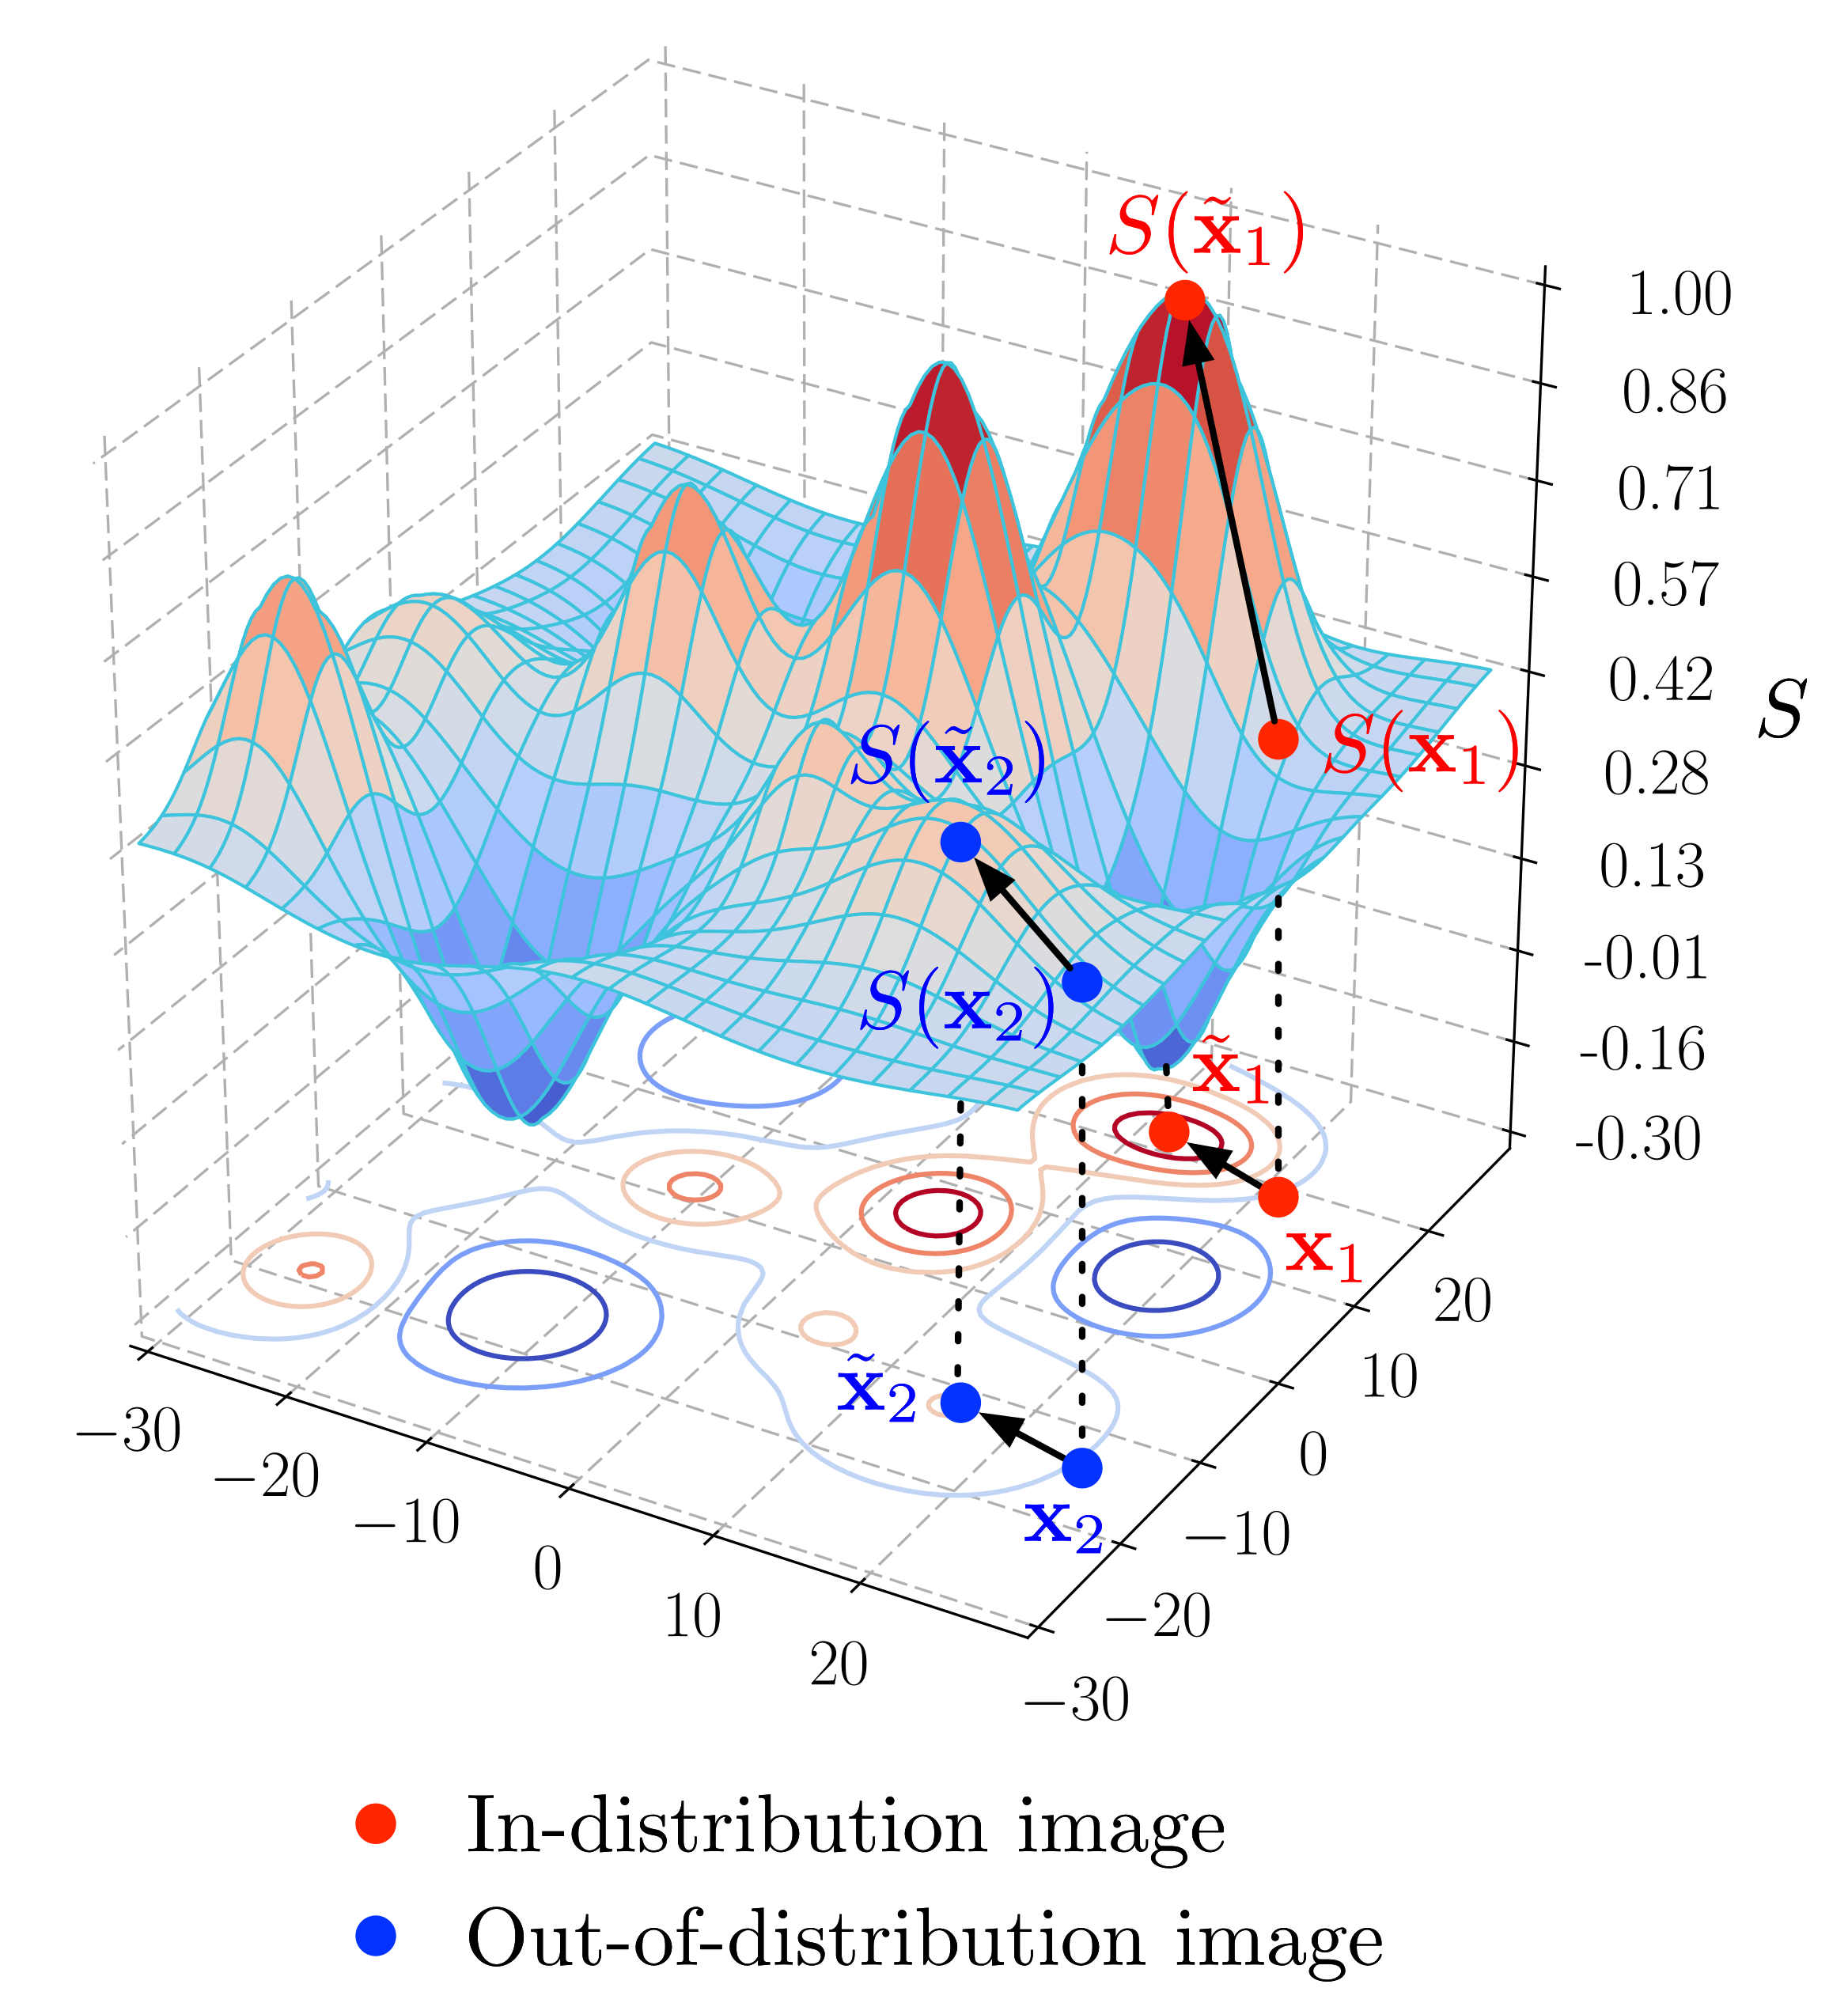
\includegraphics[width=3.25in]{figure/gradient.png}}
% \caption{Figure taken from \cite{odin}, showing the difference in gradients between ID and \ac{ood} data points}
% \label{softmaxmove}
% \end{figure}
%
% The interpretation of the temperature scaling is slightly more complex. By performing a Taylor expansion and omitting third and higher orders, we can rewrite the softmax score (i.e the value of the predicted class, the highest value) as ${S\propto {(U_{1}-U_{2}/2T)/T}}$, with $U_1$ and $U_2$ defined as follows \cite[4]{odin}:
%
%
% \begin{equation}\label{eq::u1u2}
% U_{1}(\bm{x})=\frac{1}{N-1}\sum_{i\neq\hat{y}}[f_{\hat{y}}(\bm{x})-f_{i}(\bm{x})]
% \end{equation}
%
% \begin{equation}\label{eq::u1u2}
% U_{2}(\bm{x})=\frac{1}{N-1}\sum_{i\neq\hat{y}}[f_{\hat{y}}(\bm{x})-f_{i}(\bm{x})]^{2}
% \end{equation}
%
% $\hat{y}$ is the predicted class, and is thus also the index for the highest value in $f(\bm{x})$. Thus, $U_1$ represents "the extent to which the largest unnormalized output deviates from the remaining outputs", while $U_2$ measures how the remaining outputs deviate from each other \cite[6]{odin}.
%
% \cite{odin} makes the two following observations with regards to these two values: Firstly, they find that the largest unnormalized output tends to deviate more for ID samples, making $U_1$ larger than for \ac{ood} samples, because the model is more confident in its prediction. Secondly, they find that $E[U_2|U_1]$ is larger for ID data samples than for \ac{ood} samples, which shows that ID samples have more separation in the remaining unnormalized inputs than \ac{ood} samples. 
%
% Returning to the Taylor approximated softmax score ${S\propto {(U_{1}-U_{2}/2T)/T}}$, we see that $U_1$ contributes to making the softmax score higher, while $U_2$ reduces the softmax score. Given that both these values are higher for ID data, we will want to reduce the impact of $U_2$ and increase the impact of $U_1$. As $U_1$ is divided by $T$, while $U_2$ is divided by $2T^2$, increasing the temperature achieves this, as $U_2$ will decrease much faster than $U_1$. Thus, we can see how an increased temperature increases the softmax scores for ID data, and thus increases the gap between softmax scores for ID and \ac{ood} samples, making them easier to differentiate.
%
% With these two modifications to the simple baseline proposed by \cite{oodbaseline}, \cite{odin} manages to increase the gap between the softmax scores of ID and \ac{ood} data and thus facilitates much more effective \ac{ood} detection.
% \\
%
% \subsubsection{Energy Based \ac{ood} Detection}
%
% \cite{energy} proposes using an {\it energy score} as opposed to the softmax score. They show mathematically that "the softmax confidence score is a biased scoring function that is not aligned with the density of the inputs" \cite{energy}, and thus seek to use a different measurement which is better aligned with the probability density.
%
% An energy function is a function $E(\bm{x}) : \mathbb{R}^D \rightarrow \mathbb{R}$ which maps any data point into a non-probabilistic scalar called energy. Energy values can be converted to probabilities using the Gibbs distribution defined below (equation \ref{energy}):
%
% \begin{equation} \label{energy}
%     p(y \mid \*x) = \frac{e^{-E(\*x,y)/T}}{\int_{y'} e^{-E(\*x, y')/T}}
%     = \frac{e^{-E(\*x,y)/T}}{e^{-E(\*x)/T}},
% \end{equation}
%
% This equation is quite similar to the softmax function, and we can see that by defining $E(\bm{x}, y) = -f_y(x)$. We can write the Gibbs distribution as the normal softmax output of a neural network:
%
% \begin{equation}\label{eq:softmax}
%     p(y \mid \*x) = \frac{e^{f_y(\*x)/T}}{\sum_{i}^K e^{f_{i}(\*x)/T}},
% \end{equation}
%
% By using the {\it Helmholtz free energy} measurement, we can get an energy score for each data point given to the model, which can be used to detect \ac{ood} data points. Given that we define $E(\bm{x}, y) = -f_y(x)$, we can write the Helmholtz free energy $E(\bm{x})$ as:
%
% \begin{equation}\label{eq:energy_softmax}
%   E(\*x;f)=- T\cdot \text{log}\sum_i^K e^{f_i(\*x)/T}.
% \end{equation}
%
% The authors show that when training with negative log likelihood loss, the optimization will reduce the free energy of ID data points, and that the difference  between ID and \ac{ood} energy scores is higher than the difference in softmax scores \cite{energy}. Thus, thresholding the free energy function is an effective way to separate ID and \ac{ood} data points. Furthermore, they also present a method for fine tuning a pre trained model using a loss function that is based on the energy score. By doing this, the gap between ID and \ac{ood} energy scores can be increased even further.
% \\
%
% \subsubsection{ReAct}
%
% ReAct \cite{react} is a very simple method, which also aims to increase the difference in confidence scores between ID and \ac{ood} data. It does this by rectifying high activations in the penultimate layer, which surprisingly achieves this very effectively. Figure \ref{react} gives an intuition for why this is the case:
%
% \begin{figure}[h]
% \centerline{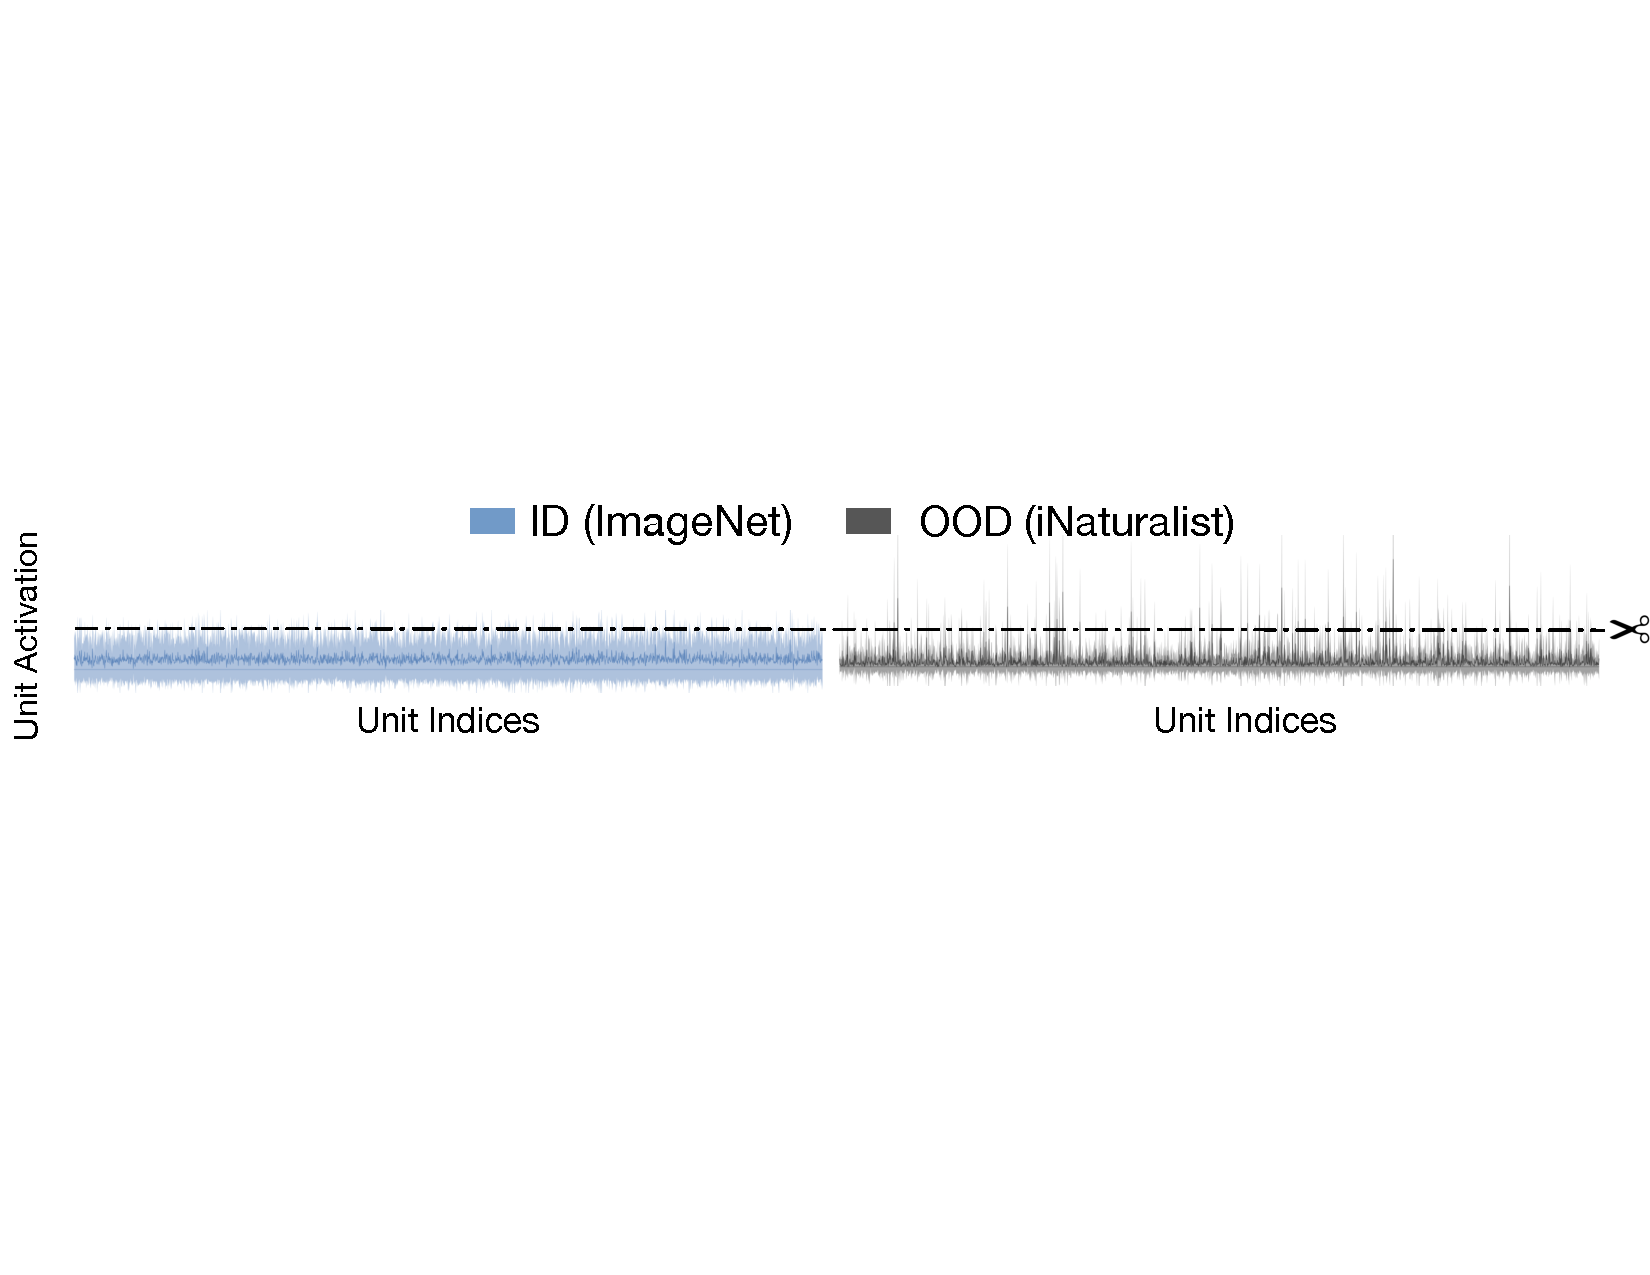
\includegraphics[width=3.25in]{figure/react.pdf}}
% \caption{Figure taken from \cite{react}, showing the activations for the nodes in the penultimate layer for ID and \ac{ood} data}
% \label{react}
% \end{figure}
%
% From this, we see that \ac{ood} samples have much more irregular activations, with a higher variance and many high value outliers. This gives an explanation for why \ac{ood} samples produce highly confident softmax scores: sharp positive outliers manifest in the model output, producing high logits in the output layer \cite{react}. By using a positive upper limit to rectify these outliers, we can remove their impact and reduce the confidence for \ac{ood} data.
%
% This gives rise to a very simple \ac{ood} detector: Let us denote the feature vector of the penultimate layer as $h(\bm{x})$, where $\bm{x}$ is the input feature vector. The logits of the network would be calculated by the function
%
% \begin{equation}\label{dog}
%   f(\bm{x}) = W \, h(\bm{x}) + \bm{b},
% \end{equation}
%
% where $W$ is a matrix which projects $h(\bm{x})$ down to the output space. $h(\bm{x})$ is the vector which contains the high activations for \ac{ood} data, so by rectifying this vector with $\text{ReAct}(\bm{x}; c) = min(\bm{x}, c)$ for a $c > 0$, we can remove these outlier activations. We then get
%
% \begin{equation}\label{dog}
%   \bar{h}(\bm{x}) = \text{ReAct}(h(\bm{x}; c),
% \end{equation}
%
% which gives us the new output logits 
%
% \begin{align}
% f^{\text{ReAct}}(\*x;\theta) = \*W^\top \bar h(\*x) + \mathbf{b}.
% \end{align}
%
% These logits can be used by any other \ac{ood} method which uses the output values to separate ID and \ac{ood} samples \cite{react}:
%
% \begin{align}
% \label{eq:threshold}
%     g(\bm{x}; f^\text{ReAct}, \delta)=\begin{cases} 
%         \text{in } & S(\bm{x};f^\text{ReAct})\ge \delta \\
%         \text{out} & S(\bm{x};f^\text{ReAct}) < \delta 
%    \end{cases},
% \end{align}
%
% This simple methods performs well on many benchmarks, with the added benefit that it can be combined with many other methods. For example, we can use ODIN or Energy with output scores calculated using ReAct instead of unrectified outputs, which leads to improvements over the methods used by themselves.
% \\
%
% \subsubsection{Virtual Outlier Synthesis (VOS)}
%
% Generating outliers to expose to the model during training is another way to reduce the model's confidence on \ac{ood} data. However, creating realistic \ac{ood} data points can be difficult, especially if the input space is of a high dimension, such as in image classification. \cite{vos} presents a more tractable method, which synthesizes outliers not in the input space, but in the feature space, which can be of a much lower dimensionality.
%
% In this lower dimension space, previously intractable methods are now less computationally expensive. To synthesize outliers, \cite{vos} simply estimates class conditional Gaussian distributions by computing empirical class means and covariances, and sample outliers from the class boundaries between these Gaussians.
%
% Using these outliers, they present a "unknown-aware training objective", which can be used during training to maximize the separability between ID and \ac{ood} data during inference.
% \\
%
% \subsubsection{GradNorm}
%
% As opposed to using the feature or output space, GradNorm \cite{gradnorm} attempts to use the gradient space of a network to calculate \ac{ood}-ness. They find that the gradients of the weights actually contain valuable information that allows for effective separation of ID and \ac{ood} samples, and perform ablation studies which show that this methods outperforms many other methods, including the previously mentioned ODIN and Energy methods.
%
% The gradients are calculated with regards to the Kullback-Leibler divergence between the softmax values and a uniform distribution. An important distinction from other methods is that all the softmax values are used, as opposed to the {\it softmax score} which would be only the score of the predicted class. Thus, this method captures information about the uncertainty across all categories, as opposed to just the most likely class \cite[3]{gradnorm}. Once the gradients have been calculated, the threshold is simply done on the $L_p$-norm of these gradients, giving us the following thresholding function \cite{gradnorm}:
%
% \begin{equation}
% \label{eq:score}
%     S(\*x) = \lVert\frac{\partial D_\text{KL}(\*u~\lVert~\text{softmax}(f(\*x))}{\partial \*w}  \rVert_p
% \end{equation}
%
% As shown in figure \ref{gradnorms}, we see that the gradient norms are consistently lower for \ac{ood} data (gray) than ID data (blue).
%
% \begin{figure}[h]
% \centerline{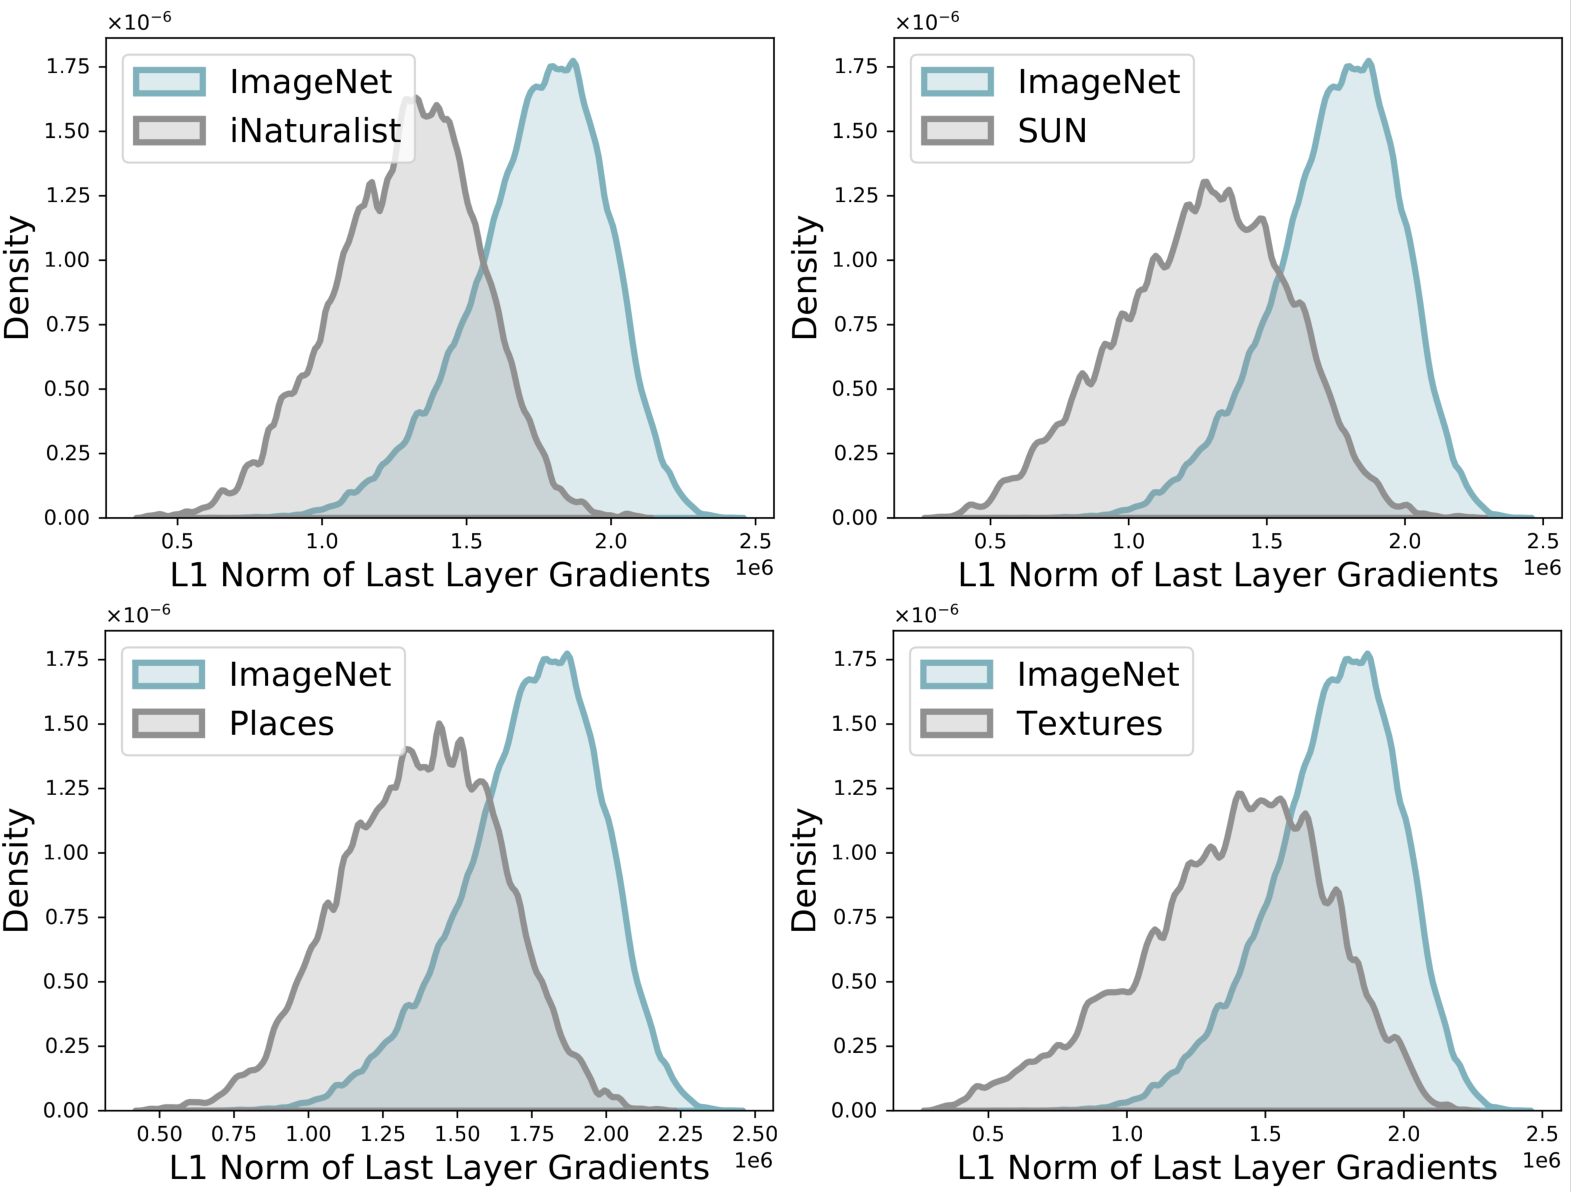
\includegraphics[width=3.25in]{figure/gradnorm.pdf}}
% \caption{Figure taken from \cite{gradnorm}, showing the difference in gradient norms between ID and \ac{ood} data}
% \label{gradnorms}
% \end{figure}
%
% \cite{gradnorm} find that it is sufficient to only calculate the gradients for the last layer of the network, and that the $L_1$-norm performs the best, as it weights all gradients equally, as opposed to higher norms which place more importance on larger values.
%
% In their mathematical analysis, they show that GradNorm captures joint information from both the feature and output space. By decomposing the $L_1$-norm of gradients of weights of the last layer with regards to the Kullback-Leibler divergence, they reach the following equality:
%
% \begin{equation}
% S(\bm{x}) = \frac{1}{CT}  \left(\sum_{i=1}^m |x_i|\right) \left(\sum_{j=1}^C \left|1 - C \cdot \frac{e^{f_j / T}}{\sum_{j=1}^C e^{{f_{j}} / T}}\right|\right)
% \label{eq:decomp}
% \end{equation}
%
% From this, we see that $S(\bm{x})$ is a product of a factor which is simply the $L_1$-norm of the feature vector $\bm{x}$, and another term which captures information about the softmax values in the output space.
% \\

\subsubsection{Virtual Logit Matching (ViM)}

\cite{vim} attempts to improve \ac{ood} detection by calculating a score based on the feature, the logit and the softmax probability at once, as opposed to just one of them. By looking at all three elements in conjunction, they see an increase in performance over models which only rely on a single input source (such as the previously mentioned ODIN).

The reasoning behind not just looking at the logits or softmax probability is that there is a lot of information that is lost when going from features to logits \cite{vim}. Once we project the features down to logits, we have only class dependent information, and have lost the class agnostic information which is contained within the features. To show how this information is lost, the authors give an example based on null space analysis \cite{nusa}:

Let us assume that we have a simplified network with only a single layer. Then, we have $\hat{\bm{y}} = W \bm{x}$, where $\hat{\bm{y}}$ is the vector containing the logits, $\bm{x}$ is the feature vector of the input (with an additional 1 for the bias term) and $W$ is the matrix containing the weights and biases transforming the feature vector into logits. A null space $\text{Null}(W)$ of a matrix $W$ is the set of all vectors that map to the zero vector, such that $W \bm{a} = \bm{0} \iff \bm{a} \in \text{Null}(W)$. The null space of a matrix may be trivial (empty), but a matrix which projects vectors to a lower dimension have non-trivial null spaces. Given that the final layer of a neural network projects down to logits, which are the same dimension as the number of classes, this will almost always be the case. Because of the distributivity of matrix multiplication, we have the following:

\begin{equation}
W (\bm{x} + \bm{a}) = W \bm{x} + W \bm{a} = W \bm{x} + \bm{0} = W \bm{x}
\label{matrix}
\end{equation}

The vector $\bm{x}$ can be decomposed into $\bm{x}^W + \bm{x}^{\text{Null}(W)}$, where $\bm{x}^W$ is the projection of $\bm{x}$ onto the column space of $W$ and $\bm{x}^{\text{Null}(W)}$ is the projection of $\bm{x}$ onto the null space of $W$. It follows from this and equation \ref{matrix} that when going from features to logits using the projection $W \bm{x}$, we lose all information contained in $\bm{x}^{\text{Null}(W)}$. \cite{nusa} shows how this can be exploited by adversarial methods, by creating images with added noise derived from the null space of a matrix within the network, which are classified as if the noise was not present, despite having no resemblance to the original image. See figure \ref{dog}.

\begin{figure}[hbt]
    \centering
    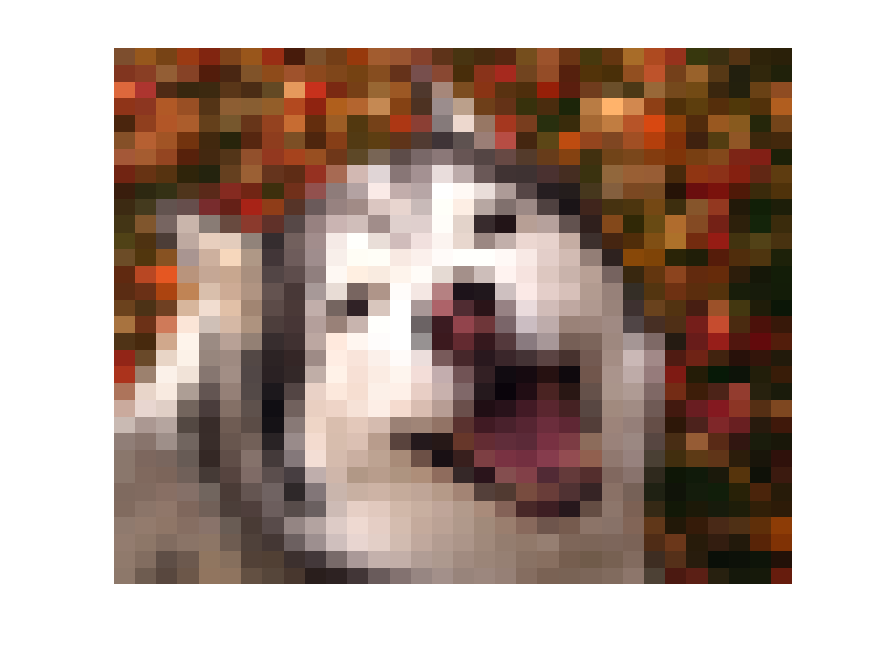
\includegraphics[width=0.32\linewidth,trim={1.25cm 1.25cm 1.25cm 1.25cm},clip]{figure/OrigImage.pdf}
    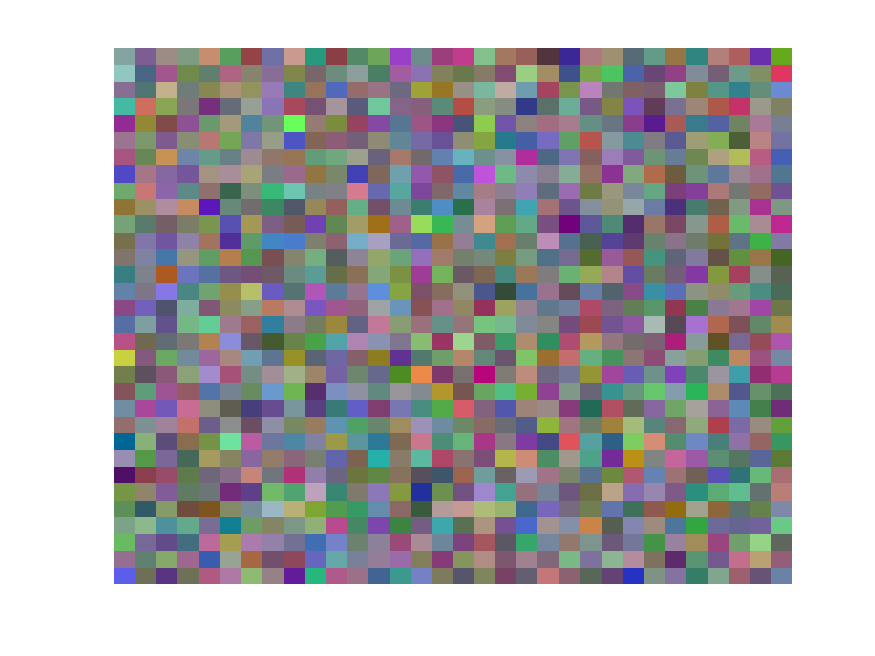
\includegraphics[width=0.32\linewidth,trim={1.25cm 1.25cm 1.25cm 1.25cm},clip]{figure/PureNoise.pdf}
    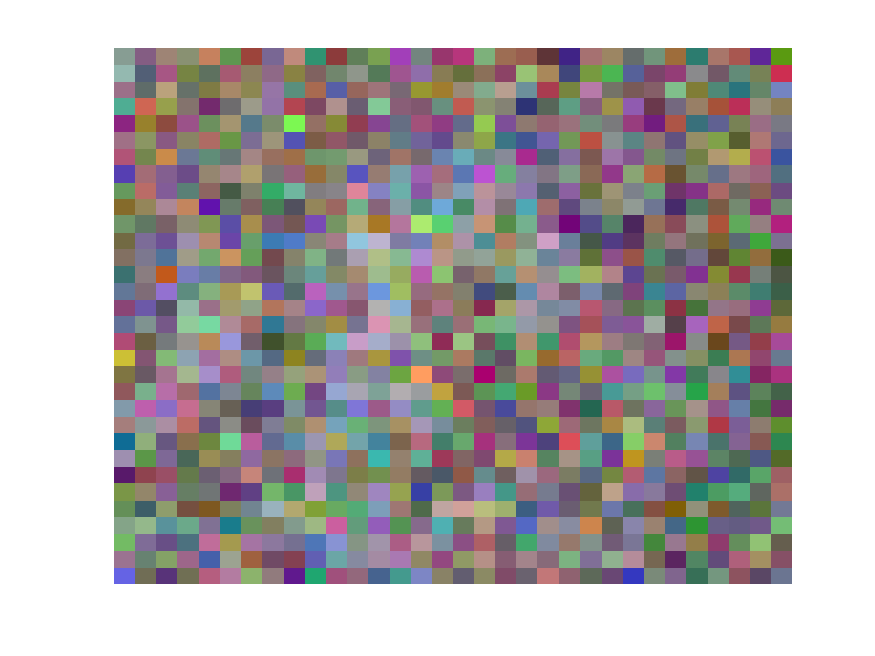
\includegraphics[width=0.32\linewidth,trim={1.25cm 1.25cm 1.25cm 1.25cm},clip]{figure/NoiseAdded.pdf}
    \caption{Image taken from \cite{nusa}. Left: Original image. Center: Additive null space noise. Right: Final image, indistinguishable from original image according to the network the noise in the center column is sampled from.}
    \label{dog}
\end{figure}

From this, we can see that potentially large amounts of information can be lost when going from features to logits. Using this information, it is also possible to perform \ac{ood} detection, as shown by \cite{nusa}. Another method which uses the features performs Principal Component Analysis (PCA) and looks at the residual information lost when using the first $N$ principal components \cite{subspace}. However, the information in the features is still class agnostic, and \cite{vim} aims to go beyond using just one input source and combine several elements of the network.

To do this, they propose using a {\it Virtual Logit}. The Virtual Logit is calculated as follows: First, they center the feature space, so that "it is bias free in the computation of logits" \cite{vim}. They then perform PCA as in \cite{subspace}, and calculate the residual of $\bm{x}$ with regards to the principal components, which is the projection $\bm{x}$ onto the null space of the principal subspace $P$. The residual represents the information lost when using the projection $P$.

\begin{equation}
\text{Residual}(x) = || \bm{x}^{\text{Null}(P)}||
\label{virtuallogit}
\end{equation}

This value is scaled based on the average values of the maximum logit across the dataset, and is appended to the rest of the logits as a Virtual Logit:

\begin{equation}
l_0 := \alpha || \bm{x}^{\text{Null}(P)}||
\label{virtuallogit}
\end{equation}

This now takes part in the computation of the softmax values, and thus is affected by the size of the rest of the logits. They call the softmax value of the Virtual Logit the {\it ViM score}. In this way, the ViM score represents the size of the residual in comparison with the predictions of the model. If the model is very confident, then the norm of the residual will be small in comparison, and the ViM score will be low. If the residual is very large, the ViM score will be higher, and more indicative of an \ac{ood} sample. In this way, \cite{vim} have combined information from the feature, the logit and the softmax probability level to perform \ac{ood} detection.

\section{Related work} \label{section:relatedwork}

While the combination of \ac{xai} and \ac{ood} detection has been explored in many previous works, the majority of them focus on explaining why a data point was marked as \ac{ood}, as opposed to using \ac{xai} to aid the detection itself. Works like \cite{uncertainty}, \cite{generalxaiforood} and \cite{tallon2020explainable} are papers which combine \ac{xai} and \ac{ood} for this purpose. Within network security, \ac{xai} has been as part of anomaly detection systems to detect malicious or faulty network traffic. Here, it has been used to explain detections (\cite{idsxai}, \cite{mahbooba}), but also to aid in detection itself by inspecting the explanations of the detection system (\cite{tcydenova2021detection}, \cite{dnsxai}). These methods thus use \ac{xai} to aid \ac{ood} detection in a similar manner to my work, however they are strictly focused on sequential network traffic data as opposed to images, and are mostly concerned with detection "unnatural" data samples such as intentionally malicious traffic or that generated by faulty equipment, as opposed to natural \ac{ood} data caused by semantic or covariate shift occurring when a model is deployed.

\cite{martinez} is the most relevant previous work. Here, the authors explicitly aim to use \ac{xai} to improve \ac{ood} detection on images. They do this by looking at saliency maps produced by a \ac{gradcam}-based \ac{xai} method (section \ref{section:gradcam}) during inference, i.e the heatmaps that explain which parts of the image was most influential to classify the image as a specific class. Using these heatmaps, they perform distance-based \ac{ood} detection (section \ref{section:distancebasedood}): By collecting all explanations for each image in the ID dataset, they are able to construct archetypical explanations, and can make clusters of explanations. To perform \ac{ood} detection, they simply compare the explanation of a new data point to the clusters of archetypical explanations, and mark it as \ac{ood} if it has a distance which is over a certain threshold.

This method performs decently on toy datasets, achieving scores similar to State-of-the-Art methods when using {\it Fashin MNIST} as ID and {\it MNIST} as \ac{ood}. However, this method fails catastrophically in more complicated scenarios, achieving an AUROC score of only $52\%$ on {\it CIFAR10} vs {\it SVHN}, which is only marginally better than pure guessing and far below any other method. The paper thus ends with the authors concluding that "OoD detection approaches that are specifically designed for the purpose achieve in general better detection scores at the cost of an additional computational burden in the model’s construction" \cite{martinez}.

For more potential related work, we can look to OpenOOD (\cite{openood}), which aims to provide a comprehensive benchmark of all relevant methods in the field of \ac{ood} detection. Out of all 41 \ac{ood} detection methods included in this benchmark, there are no methods which use \ac{xai}.

From the absence of any relevant method utilizing \ac{xai} in OpenOOD and from the poor results of \cite{martinez}, we can see that the potential for a truly effective \ac{ood} detection system using \ac{xai} has not been fully realized in any previous work.

\section{Summary}

In this chapter, I have given a thorough introduction.

\chapter{Methodology}

The core of this work is the 

As shown in the preceding chapter, there exists a plethora of \ac{xai} methods, which exploit gradient information, differences in output scores when altering model inputs, marginal contributions of input features, as well as many other intricacies of deep learning models. The core idea of this master thesis is that these methods, in their attempt to explain a model decision, may also inadvertently extract information which is valuable for \ac{ood} detection. Thus, there may be an unexplored potential in these methods to function not just as explanations, but also as classifiers which allow us to separate ID and \ac{ood} data. Intuitively, we might expect the explanations to be more spread out on \ac{ood} images, given that there are (by definition) no objects of interest in the image that the model can definitely be said to focus on. In contrast, we might expect an explanation on an ID image to be more focused on a specific area, which contains an object of interest. Furthermore, given that saliency methods give a numerical value to each region of the image, we might be able to extract information about the "\ac{ood}-ness" of an image by inspecting the magnitudes of these values. Intuitively, it makes sense that such values should be lower for \ac{ood} than ID, reflecting the higher uncertainty present in \ac{ood} data.

As an example, let us consider \ac{gradcam}. As explained in section \ref{section:gradcam}, \ac{gradcam} uses the gradients of the weights within the final convolutional layer with regard to the output prediction, along with the final feature maps, to generate an explanation.

\section{Proposed \ac{xai} methods for \ac{ood} detection}

In this section, I introduce my proposed methods for \ac{ood} detection, which utilize \ac{xai} methods as part of their detection pipeline.

\subsection{Stand-alone saliency methods}

As we have seen from section \ref{section:relatedwork}, there has been little research into using explanations for \ac{ood} detection, aside from the work of \cite{martinez}. Thus, I begin by presenting a simple baseline method which uses saliency values generated by \ac{xai} methods to calculate an \ac{ood} score.

\subsubsection{Aggregate of Saliency}

As mentioned previously, the field of \ac{ood} detection started with the simple baseline introduced by \cite{oodbaseline}, which simply uses the \ac{msp} (i.e the confidence score of the predicted class) as a way to measure \ac{ood}. As such, I propose a similarly simple baseline when using explanations for \ac{ood} detection. The analogue of the maximum logit in an \ac{xai} context can reasonably be said to be the explanation generated of the predicted class (the class corresponding to the maximum logit). As explained previously, this explanation will take the form of an $n \times m$ saliency map. This saliency map is not a single scalar value, and does thus not make a suitable \ac{ood} score by itself. Instead, we may perform some form of aggregation on the saliency map (such as taking the mean, the max, the variance or some other form), and use this as the \ac{ood} score.

The intuition for this method is informed by the fact that there are many forms of aggregation over saliencies which one might reasonably expect to be different for ID and \ac{ood} data. As an example, let us consider the implications of aggregating in some way which captures the magnitude of the saliencies, such as the {\it mean}, the {\it norm}, or the {\it max value}. When we generate a saliency map using the predicted class, the \ac{xai} saliency method attempts to calculate a measure of importance for each region of the input image, with regard to this class. For ID data, as long as the model predicted correctly, we know that there really are regions of the input image which contain the predicted class. If we instead are looking at semantically shifted \ac{ood} data, we know that no input image contains any of the ID classes. Thus, when a neural network makes a prediction on such a data point, it will always be wrong, because it will always predict one of the ID classes. By generating a saliency map of this prediction, we are asking a method to decide how each region contributed to a false decision. Given that there are no objects of the predicted class, in any region, we should expect the saliency values to be lower than in an ID case, where such objects actually are present.

To further illustrate this theoretical justification, I present a simple example scenario (figure \ref{fig:meansaliency}). Here, I imagine a model which has been trained to differentiate between different breeds of dogs. In the first case, it is given an image of a dog, and a prediction of "English Foxhound" is made, which happens to be correct. Generating an explanation for this prediction, each region of the image is given a measure of importance, calculated using gradient information, differences in prediction score on counterfactual examples or by other means. As there actually is an English Foxhound in the image, we expect that these methods generate saliencies which have a magnitude which is higher than if there was no dog present.

\begin{figure}[H]
    \begin{center}

    \begin{tikzpicture}[
    SIR/.style={rectangle, draw=black!60, thick, minimum size=5mm},
    ]

    \node[SIR, label={[align=center]Image with dog present,\\correctly classified as\\"English Foxhound"}] (idimg) {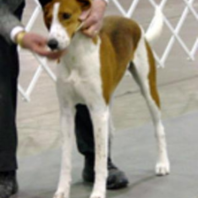
\includegraphics[width=0.25\textwidth]{figure/meansaliency/meansaliency0.png}};
    \node[SIR, label={[align=center]Image without dog\\present, wrongly\\classified as "Samyoed"}] (oodimg) [right=of idimg] {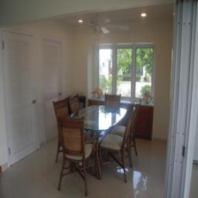
\includegraphics[width=0.25\textwidth]{figure/meansaliency/meansaliency2.png}};

    \node[SIR] (idsal) [below=1.5cm of idimg] {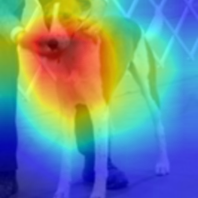
\includegraphics[width=0.25\textwidth]{figure/meansaliency/meansaliency1.png}};
    \node[SIR] (oodsal) [below=1.5cm of oodimg] {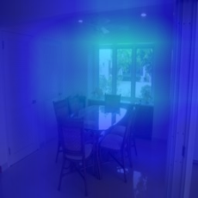
\includegraphics[width=0.25\textwidth]{figure/meansaliency/meansaliency3.png}};

    \node[SIR] (idmean) [below=1.5cm of idsal] {Mean saliency = $0.152$};
    \node[SIR] (oodmean) [below=1.5cm of oodsal] {Mean saliency = $0.034$};

    \draw[->, very thick] (idimg.south)  to node[midway, fill=white, align=center] {Generate \ac{xai} heatmap\\of model prediction} (idsal.north);
    \draw[->, very thick] (oodimg.south)  to node[midway, fill=white, align=center] {Generate \ac{xai} heatmap\\of model prediction} (oodsal.north);

    \draw[->, very thick] (idsal.south)  to node[midway, fill=white, align=center] {Calculate average value\\of heatmap} (idmean.north);
    \draw[->, very thick] (oodsal.south)  to node[midway, fill=white, align=center] {Calculate average value\\of heatmap} (oodmean.north);

    \node[SIR, align=left, draw=id, fill=id!30] (iddecision) [below=of idmean] {Above threshold:\\classified as ID};
    \node[SIR, align=left, draw=far, fill=far!30] (ooddecision) [below=of oodmean] {Below threshold:\\classified as \ac{ood}};

    \draw[->, very thick] (idmean.south)  to node[midway, fill=white] {Compare with threshold} (iddecision.north);
    \draw[->, very thick] (oodmean.south)  to node[midway, fill=white] {Compare with threshold} (ooddecision.north);

    \end{tikzpicture}

    \caption[Mean Saliency visual explanation]{Figure showing the functioning of the Aggregate of Saliency \ac{ood} detector, using mean as the aggregation, in a hypothetical scenario where a model trained on images of dogs is shown an image with no dogs present}
    \label{fig:meansaliency}

    \end{center}
\end{figure}

In the second case, the model is given an image without any dogs present. Given that there is no class for images without dogs in them, the model will classify the image as one of the possible dog breeds. In this case, the model predicted the class of "Samoyed", a decision which can be considered essentially arbitrary. When a explanation is generated for this decision, the methods for calculating importance scores will most likely assign saliencies to most regions, given that no region contains a dog. As such, if we calculate mean saliencies for both the image with the dog and the one without, we expect the image with the dog to have a higher mean saliency. As long as we work with semantically shifted \ac{ood} data, it will always be the case that the prediction on \ac{ood} data is wrong, and thus we may also expect that the generated explanations in general output lower saliencies.

Apart from aggregations which convey information about the magnitude of the saliencies, we may also expect the variation or spread of the saliencies to be different between ID and \ac{ood} data. The intuition is that one might expect the heatmap on \ac{ood} data to be less concentrated and more spread out, given that there are no actual objects of interest present.

Figure \ref{fig:varsaliency} shows a hypothetical scenario in which calculating the spread could be beneficial in \ac{ood} detection. Like in the previous case, we imagine a model trained on dogs, which is fed two images, one which contains a dog and one which does not. In this case, we do not care about the magnitudes, but instead only the spread of the values in relation to each other, and thus the heatmap is normalized. As we can see, the heatmap is more spread out in the explanation where there is no dog present than for the image with a dog. By calculating a suitable metric, such as the Gini coefficient, entropy or another measure of spread, we can get a single number which represents how spread out the heatmap is, regardless of its magnitude. Using these values, we can define a threshold which is below most ID data and above most \ac{ood} data, allowing us to separate these distributions.

\begin{figure}[H]
    \begin{center}

    \begin{tikzpicture}[
    SIR/.style={rectangle, draw=black!60, thick, minimum size=5mm},
    ]

    \node[SIR, label={[align=center]Image with dog present,\\correctly classified as\\"Golden Retriever"}] (idimg) {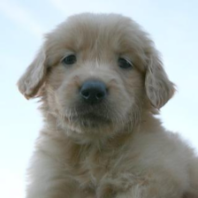
\includegraphics[width=0.25\textwidth]{figure/varsaliency/varsaliency0.png}};
    \node[SIR, label={[align=center]Image without dog\\present, wrongly\\classified as "Dingo"}] (oodimg) [right=of idimg] {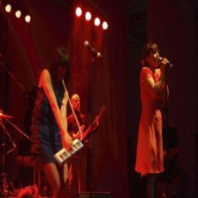
\includegraphics[width=0.25\textwidth]{figure/varsaliency/varsaliency2.png}};

    \node[SIR] (idsal) [below=1.5cm of idimg] {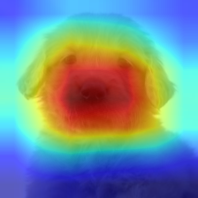
\includegraphics[width=0.25\textwidth]{figure/varsaliency/varsaliency1.png}};
    \node[SIR] (oodsal) [below=1.5cm of oodimg] {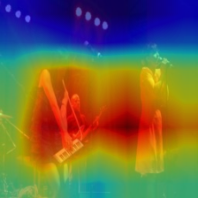
\includegraphics[width=0.25\textwidth]{figure/varsaliency/varsaliency3.png}};

    \node[SIR] (idmean) [below=1.5cm of idsal] {GINI = $0.6$};
    \node[SIR] (oodmean) [below=1.5cm of oodsal] {GINI = $0.2$};

    \draw[->, very thick] (idimg.south)  to node[midway, fill=white, align=center] {Generate \ac{xai} heatmap\\of model prediction} (idsal.north);
    \draw[->, very thick] (oodimg.south)  to node[midway, fill=white, align=center] {Generate \ac{xai} heatmap\\of model prediction} (oodsal.north);

    \draw[->, very thick] (idsal.south)  to node[midway, fill=white, align=center] {Calculate variance\\of heatmap} (idmean.north);
    \draw[->, very thick] (oodsal.south)  to node[midway, fill=white, align=center] {Calculate variance\\of heatmap} (oodmean.north);

    \node[SIR, align=left, draw=id, fill=id!30] (iddecision) [below=of idmean] {Above threshold:\\classified as ID};
    \node[SIR, align=left, draw=far, fill=far!30] (ooddecision) [below=of oodmean] {Below threshold:\\classified as \ac{ood}};

    \draw[->, very thick] (idmean.south)  to node[midway, fill=white] {Compare with threshold} (iddecision.north);
    \draw[->, very thick] (oodmean.south)  to node[midway, fill=white] {Compare with threshold} (ooddecision.north);

    \end{tikzpicture}

    \caption[Spred of Saliency visual explanation]{Figure showing the functioning of the Spread of Saliency \ac{ood} detector in a hypothetical scenario where a model trained on images of dogs is shown an image with no dogs present}
    \label{fig:varsaliency}
    \end{center}
\end{figure}

With the intuition explained, we may now formalize the method. To define this detector mathematically, let us first define the necessary components. As in chapter \ref{chapter:background}, we assume we have a model $f: \bm{x} \to \R^C$. In this case, $\bm{x} \in \R^{D \times H \times W}$, i.e a $D$ channel image of height $H$ and width $W$. In addition, we define a \ac{xai} saliency mapping method $s: (f, \bm{x}) \to \R^{H_s \times W_s}$. This function takes the model $f$ and an input $\bm{x}$ and returns a $H_s$ by $W_s$ saliency map for the predicted class; the class corresponding to the highest logit. Finally, we define an aggregation function $A: \bm{x} \rightarrow \R$, where $\bm{x}$ can be of any shape.

Thus, the \ac{ood} detector has the following form, given a threshold $\delta$:

\begin{align}
    g(\bm{x}; s, A, \delta)=\begin{cases} 
        \text{in } & A(s(\bm{x}, f)) \ge \delta \\
        \text{out} & A(s(\bm{x}, f)) < \delta 
   \end{cases}
\label{eq:aggregate}
\end{align}

% Algorithm \ref{algo:meansaliency} shows the pseudo-code for the Mean Saliency \ac{ood} Detector. Like the baseline Maximum Softmax and Logit methods introduced by \cite{oodbaseline} and \cite{mls}, it is very simple:
%
% \begin{algorithm}
%     \caption{Mean Saliency \ac{ood} Detector}
%     \label{algo:meansaliency}
%     \begin{algorithmic}
%     \Require Trained Neural Network $f$, Saliency Method $s$, Input Data Sample $x$
%     \Ensure ID Score
%
%     \Function{mean\_saliency}{$f$, $s$, $x$}
%         \State $pred \gets f(x)$
%         \State $class \gets \arg\max(pred)$
%         \State $saliency\_map \gets s(f, x, class)$
%         \State $id\_score \gets \text{mean}(saliency\_map)$
%         \State \Return $id\_score$
%     \EndFunction
%
%     \end{algorithmic}
% \end{algorithm}




% Below (algorithm \ref{algo:varsaliency}), we see the pseudo-code for the Spread of Saliency \ac{ood} Detector, which is equivalent to the Mean Saliency method apart from the aggregation of each saliency map being a measure of spread as opposed to the mean.
%
%
% \begin{algorithm}
%     \caption{Spread of Saliency \ac{ood} Detector}
%     \label{algo:varsaliency}
%     \begin{algorithmic}
%     \Require Trained Neural Network $f$, Saliency Method $s$, Measure of Spread $\sigma$, Input Data Sample $x$
%     \Ensure ID Score
%
%     \Function{spread\_of\_saliency}{$f$, $s$, $\sigma$, $x$}
%         \State $pred \gets f(x)$
%         \State $class \gets \arg\max(pred)$
%         \State $saliency\_map \gets s(f, x, class)$
%         \State $id\_score \gets \sigma(saliency\_map)$
%         \State \Return $id\_score$
%     \EndFunction
%
%     \end{algorithmic}
% \end{algorithm}




\subsubsection{Explanation Clustering}


\subsection{Saliency integrated into existing \ac{ood} detection algorithms}

Given the poor results of \cite{martinez}, one might expect that saliency maps on their own are insufficient to differentiate ID and \ac{ood} data.

\subsubsection{Virtual Logit Matching with Saliencies}


\section{Datasets} \label{section:datasets}

With a thorough introduction to both \ac{xai} and \ac{ood} detection as well as methods which combine the two, I shall present the datasets that will be used to test the new method that I introduce in chapter \ref{chapter:newmethod}. The two datasets used are OpenOOD (\cite{openood}) and HyperKvasir (\cite{hyperkvasir}). OpenOOD is a comprehensive benchmark which can test the new method's performance in a wide range of \ac{ood} scenarios, while HyperKvasir is a medicinal dataset which can be used to test the method in the specific use case of gastrointestinal \ac{ood} detection.


\subsection{OpenOOD} \label{chapter:openood}

As mentioned previously, OpenOOD was introduced in 2023 by \cite{openood} as an attempt to unify the performance metrics of the field, such that accurate comparisons of different methods could be made. Prior to this work, different methods were tested on different datasets, with different image preprocessing procedures, and with other externalities which inhibited effective comparison between methods \cite{openood}.

OpenOOD includes 11 different benchmarks across Anomaly Detection, Open Set Recognition and \ac{ood} detection, three fields which are very closely related. Of these, 6 benchmarks are used to test methods for \ac{ood} detection. Each benchmark is defined by an ID dataset, with 6 or more corresponding \ac{ood} datasets, separated into Near-\ac{ood} and Far-\ac{ood}.

\subsubsection{CIFAR10}

CIFAR10 \cite{cifar} is a 10-class dataset for general object recognition \cite{openood}. This dataset is commonly used in \ac{ai} research \cite{pouyanfar2018survey}. Each image is $32 \times 32$, and there are 50 000 training images and 10 000 test images. The ten classes are as follows: airplanes, cars, birds, cats, deer, dogs, frogs, horses, ships, and trucks. OpenOOD presents a series of Near-\ac{ood} and Far-\ac{ood} datasets which are used in conjunction with this dataset for evaluation. Table \ref{table:cifar10} presents a short description of each dataset and the number of samples.

\begin{table}
\begin{center}
\begin{tabular}{ |c|c|c| } 
    \hline
    Dataset & Size & Description \\
    \hline
    \rowcolor{id!50}
    CIFAR10 & 10 000 & General objects \\ 
    \hline
    \rowcolor{near!50}
    CIFAR100 & 10 000 & General objects from same collection as CIFAR10 \\ 
    \rowcolor{near!50}
    TinyImageNet & 10 000 & General objects \\ 
    \hline
    \rowcolor{far!50}
    MNIST & 10 000 & Handwritten digits from 0 to 9 \\ 
    \rowcolor{far!50}
    SVHN & 10 000 & Street view house numbers \\ 
    \rowcolor{far!50}
    Texture & 10 000 & Street view house numbers \\ 
    \rowcolor{far!50}
    Places365 & 10 000 & Places, scenes, locations \\ 
    \hline
    \end{tabular}
    \caption{Hello}
    \label{table:cifar10}
\end{center}
\end{table}

In addition, a sample of images from CIFAR10 and the corresponding \ac{ood} datasets are shown in figure \ref{fig:cifar10}.

\begin{figure}[H]
    \begin{center}

    \begin{tikzpicture}[
    SIR/.style={rectangle, draw=black!60, thick, minimum size=5mm},
    ]


    % Define the size of each image cell
    \def\cellwidth{2.3cm}
    \def\cellheight{2.3cm}
    \def\rowpadding{0.8cm}

    \pgfmathtruncatemacro{\offset}{\cellheight + \rowpadding}

    % Loop through the grid
    \foreach \row in {0, 1, 2, 3, 4, 5, 6} {
        \foreach \col in {0, 1, 2} {
            % Calculate the image number
            \pgfmathtruncatemacro{\imagenumber}{\row * 3 + \col}
            % Draw the image
            \node[inner sep=0] (\imagenumber) at (\col * \cellwidth, -\row * \offset - \cellheight) 
                {\includegraphics[width=\cellwidth, height=\cellheight]{figure/cifar10_examples/image-img\imagenumber.png}};
        }
    }
    \node [above=0.1cm of 1] {ID: CIFAR10};
    \node [above=0.1cm of 4] {Near-\ac{ood}: CIFAR100};
    \node [above=0.1cm of 7] {Near-\ac{ood}: TinyImageNet};
    \node [above=0.1cm of 10] {Far-\ac{ood}: MNIST};
    \node [above=0.1cm of 13] {Far-\ac{ood}: SVHN};
    \node [above=0.1cm of 16] {Far-\ac{ood}: Texture};
    \node [above=0.1cm of 19] {Far-\ac{ood}: Places365};

    \begin{scope}[on background layer={color=id!50}]
        \fill (-1.5,-0.4) rectangle (6.2,-3.6);
    \end{scope}

    \begin{scope}[on background layer={color=near!50}]
        \fill (-1.5,-3.6) rectangle (6.2,-9.8);
    \end{scope}

    \begin{scope}[on background layer={color=far!50}]
        \fill (-1.5,-9.8) rectangle (6.2,-22.3);
    \end{scope}

    \end{tikzpicture}

    \caption[CIFAR10 dataset example images]{Figure showing three example images from CIFAR10 and from the corresponding \ac{ood} datasets}
    \label{fig:cifar10}

    \end{center}
\end{figure}



\subsubsection{ImageNet200}

\begin{figure}[H]
    \begin{center}

    \begin{tikzpicture}[
    SIR/.style={rectangle, draw=black!60, thick, minimum size=5mm},
    ]


    % Define the size of each image cell
    \def\cellwidth{2.3cm}
    \def\cellheight{2.3cm}
    \def\rowpadding{0.8cm}

    \pgfmathtruncatemacro{\offset}{\cellheight + \rowpadding}

    % Loop through the grid
    \foreach \row in {0, 1, 2, 3, 4, 5} {
        \foreach \col in {0, 1, 2} {
            % Calculate the image number
            \pgfmathtruncatemacro{\imagenumber}{\row * 3 + \col}
            % Draw the image
            \node[inner sep=0] (\imagenumber) at (\col * \cellwidth, -\row * \offset - \cellheight) 
                {\includegraphics[width=\cellwidth, height=\cellheight]{figure/imagenet200_examples/image-img\imagenumber.png}};
        }
    }
    \node [above=0.1cm of 1] {ID: ImageNet200};
    \node [above=0.1cm of 4] {Near-\ac{ood}: SSB-Hard};
    \node [above=0.1cm of 7] {Near-\ac{ood}: NINCO};
    \node [above=0.1cm of 10] {Far-\ac{ood}: iNaturalist};
    \node [above=0.1cm of 13] {Far-\ac{ood}: Texture};
    \node [above=0.1cm of 16] {Far-\ac{ood}: OpenImage-O};

    \begin{scope}[on background layer={color=id!50}]
        \fill (-1.5,-0.4) rectangle (6.2,-3.6);
    \end{scope}

    \begin{scope}[on background layer={color=near!50}]
        \fill (-1.5,-3.6) rectangle (6.2,-9.8);
    \end{scope}

    \begin{scope}[on background layer={color=far!50}]
        \fill (-1.5,-9.8) rectangle (6.2,-19.1);
    \end{scope}

    \end{tikzpicture}

    \caption[ImageNet200 dataset example images]{Figure showing three example images from ImageNet200 and from the corresponding \ac{ood} datasets}
    \label{fig:imagenet200}

    \end{center}
\end{figure}
\begin{table}

\begin{center}
\begin{tabular}{ |c|c|c| } 
    \hline
    Dataset & Size & Description \\
    \hline
    \rowcolor{id!50}
    ImageNet200 & 10 000 & General objects \\ 
    \hline
    \rowcolor{near!50}
    SSB-Hard & 10 000 & General objects \\ 
    \rowcolor{near!50}
    NINCO & 10 000 & General objects \\ 
    \hline
    \rowcolor{far!50}
    iNaturalist & 10 000 & Handwritten digits from 0 to 9 \\ 
    \rowcolor{far!50}
    Texture & 10 000 & Street view house numbers \\ 
    \rowcolor{far!50}
    OpenImage-O & 10 000 & General objects \\ 
    \hline
    \end{tabular}
    \caption{Hello}
    \label{table:imagenet200}
\end{center}
\end{table}

\subsection{HyperKvasir} \label{chapter:hyperkvasir}

HyperKvasir is the largest gastrointestinal (GI) machine learning datasets, containing $110 \,079$ images and $374$ videos collected during gastro- and colonoscopy examinations \cite{hyperkvasir}. It is of utmost importance to detect and correctly classify disease found in the GI-tract, as the different diseases can range from minor annoyances to highly deadly diseases such as GI-cancer, which has a mortality rate of $63 \%$ \cite{hyperkvasir}. Furthermore, the effectiveness of endoscopy in locating these diseases is highly dependent on the skill and knowledge of the human operator, with polyps in the colon having a $20 \%$ miss rate \cite{kaminski2010quality}. Thus, this is a field which could benefit greatly from computer aided diagnosis, but such an integration requires robust and trustworthy AI-systems which do not make erroneous decisions with high confidence. This makes HyperKvasir an ideal dataset to test a new \ac{ood} detection method in a more practical real-world scenario.

Of the $100 \, 079$ images, $10 \, 662$ have been labeled, with a total of 23 classes. HyperKvasir also contains segmentations and labeled video, however, I shall limit myself to the labeled images and to the task of classification, as per the scope of this thesis as outlined in section \ref{section:scope}.

\section{Networks}

While it may be interesting to see how these new methods function on different network architectures, the combination of several different novel \ac{ood} detection algorithms and three different datasets already presents a considerable amount of evaluation. Thus, to focus the thesis on comparing different \ac{ood} detection methods against each other, I believe it is best to fix other parameters such as network architecture. With this in mind, I choose to limit myself to the ResNet \cite{resnet} family of neural networks. In particular, I use ResNet18 for all tests, either one trained on $32 \times 32$ images (for Cifar10), or one trained on $224 \times 224$ images (for ImageNet200, HyperKvasir).

Aside from \acp{cnn}, Vision Transformers also perform exceptionally on computer vision tasks, and achieve state-of-the-art results in many settings \cite{vit}. On ImageNet, they are even dominant, and the top 10 models when considering (top-1) accuracy are all based on vision transformers, as opposed to \acp{cnn}.\footnote{https://paperswithcode.com/sota/image-classification-on-imagenet} As such one might question the choice of a \ac{cnn} model, when newer and better models have been developed.

However, given that a large part of the \ac{xai} methods have been developed in the \ac{cnn} paradigm, they are not easily adapted to vision transformers. Methods such as \ac{gradcam} and \ac{lrp} exploit specific parts of \ac{cnn} architectures when generating explanations \cite{legrad}, and are thus difficult to use with different architectures. To be able to use a broad section of the representative \ac{xai} methods in use today, it is thus preferable to use \acp{cnn} as opposed to vision transformers.

\section{\ac{xai} Saliency Methods}

In the following section, I will describe the saliency methods I have chosen to use.

\subsection{\ac{gradcam}}

\ac{gradcam} is a natural choice of \ac{xai} method, given that is a seminal work which has inspired a large number of other methods \cite{gradcamplusplus, xgradcam, hirescam}.

% TODO: move background here?

\subsection{\ac{lime}}


\subsection{Occlusion}


\section{Evaluation}

\subsection{Metrics}

\ac{auroc} and \ac{fpr95} are the most common metrics used for \ac{ood} detection \cite{oodbaseline, odin, oodoverview, openood, vim}. In OpenOOD (\cite{openood}), \ac{auroc} is chosen as the primary metric used to rank methods against each other. As \cite{openood} by far presents the most comprehensive complete benchmark of all \ac{ood} detection methods to date, I have followed their methodology and used \ac{auroc} when evaluating my methods, while also calculating \ac{fpr95} as a secondary metric.

\ac{auroc} is agnostic to which class is the positive and which is the negative. Whether we consider \ac{ood} samples as 0 or 1, the result will be the same. However, the same is not true for \ac{fpr95}, necessitating a choice of positive and negative classes. There is no correct answer, but \cite{openood} chooses to consider \ac{ood} samples as the positive class, to "align with ML convention". It is common to consider abnormalities, anomalies, or the unexpected as the positive class (for example, a cancer detection system would consider the presence of cancer to be part of the positive class), which aligns with the goal of \ac{ood} detection. Thus, I have also followed this convention and considered \ac{ood} samples as positive, and \ac{id} samples as negative. In this case, \ac{fpr95} has the following interpretation: When 95\% of \ac{ood} samples are correctly classified as \ac{ood}, what percentage of \ac{id} samples are incorrectly classified as \ac{ood}. In other words, \ac{fpr95} measures the rate of "false alarms" when 95\% of actual anomalies are caught.

For both of these metrics, the calculations are done on each \ac{ood} dataset individually, as opposed to comparing all \ac{ood} samples to the \ac{id} dataset. Afterwards, the metrics of all Near-\ac{ood} and Far-\ac{ood} are averaged, giving us two general performance metrics which tell us how a method functions on either Near-\ac{ood} or Far-\ac{ood}.

\subsection{Development and Test Sets}

Given the scope of my thesis, which focuses on post-hoc \ac{ood} methods which do not use outlier exposure or require any form of training, there is no need for a training dataset. Despite this, there is still a chance of overfitting, due to the exploratory nature of developing an entirely new class of methods. By trying out different methods and by tuning different parameters to find out how one might best separate \ac{id} and \ac{ood} data using XAI, I am also biasing the results. Therefore, it may be possible that potential improvements in performance are not due to the increased quality of the method, but instead because of peculiarities in the specific datasets that the method is used on.

Thus, I have split all the datasets mentioned in \ref{section:datasets} into development and test sets, and have performed all development of the methods exclusively on the development set. Only when calculating the final metrics have I used the test set, to remove any bias associated with performing multiple experiments on the same data. Due to the large amount of data available in the CIFAR10 and ImageNet200 datasets, and their associated \ac{ood} datasets, I have simply split all datasets into two equally large parts.

\subsection{Bootstrapping}

When evaluating a new method, it is not enough to simply report the results from a single experiment. Instead one should run the same experiment multiple times and perform statistical analysis to ensure that the results are robust. Therefore, I have.

\section{Implementation}

This section goes over the implementation details of my thesis.

\subsection{Basic hardware and software}

Python is the most popular programming language for data science and \ac{ml} research \cite{nguyen2019machine}, and as such it is my language of choice as well. Key libraries that I have used are {\it PyTorch}, {\it OpenOOD}, {\it Captum}, {\it Matplotlib}, and others. Below is a table of the key libraries and their version numbers.

\begin{center}
    \begin{tabular}{ |c|c|c| } 
    \hline
    Library & Version number & Short description \\
    \hline
    PyTorch & 2.4.1 & GPU-accelerated \ac{ml} library \\ 
    OpenOOD & 1.5 & Comprehensive \ac{ood} detection framework \cite{openood} \\ 
    Captum & 0.7.1 & \ac{xai} methods integrated with PyTorch \\ 
    Scikit-Learn & 1.5.2 & Various \ac{ml} methods \\ 
    NumPy & 1.26.4 & Efficient matrix multiplication and scientific computing \\ 
    Matplotlib & 3.9.2  & Visualization library \\ 
    Seaborn & 0.13.2 & Visualization library based on Matplotlib \\
    \hline
    \end{tabular}
\end{center}

All development and computation was done on a single computer with an \texttt{Intel i7-8700K} CPU and an \texttt{Nvidia GeForce RTX 3090} GPU.

\subsection{Method Evaluation: OpenOOD}

As explained previously, OpenOOD \cite{openood} represents the most comprehensive benchmark for \ac{ood} detection methods. It is also a framework which easily allows for development and benchmarking of new methods, and is thus the ideal framework for the purposes of this thesis.

In particular, OpenOOD includes a "unified, easy to use evaluator" \cite{openood15} that makes evaluating new methods very simple. All that is required is that new methods inherit from a base class (\texttt{BasePostprocessor}\footnote{In OpenOOD, \texttt{Postprocessor}s are the \ac{ood} detection algorithms that generate an \ac{ood} score during inference}), and override the calculation of \ac{ood} scores. Code listing \ref{code:aggregate} shows all the code required to create the Aggregate of Saliency \ac{ood} detector.

\begin{lstlisting}[style=pythonstyle, caption={Source code listing for the Aggregate of Saliency \ac{ood} detector}, captionpos=b, label={code:aggregate}]
class SaliencyAggregatorPostprocessor(BasePostprocessor):
    def __init__(self, config, saliency_generator, aggregator):
        super().__init__(config)

        self.saliency_generator = saliency_generator
        self.aggregator = aggregator

    def postprocess(self, net: nn.Module, data: Any):
        predictions = torch.argmax(net(data), dim=-1)

        saliencies = self.saliency_generator(net, data)
        score_ood = self.aggregator(saliencies, dim=-1)

        return predictions, score_ood
\end{lstlisting}

With this \texttt{postprocessor} defined, evaluating it on a specific dataset is similarly simple (listing \ref{code:eval}):

\begin{lstlisting}[style=pythonstyle, caption={Source code listing for evaluating methods within the OpenOOD framework}, captionpos=b, label={code:eval}]
resnet18_pretrained = get_network('cifar10')

ood_detector = SaliencyAggregatorPostprocessor(None, GradCAM, torch.mean)

evaluator = Evaluator(
    net=resnet18_pretrained,
    id_name='cifar10',
    postprocessor=ood_detector,
)

metrics = evaluator.eval_ood()

print(metrics)
\end{lstlisting}

This code will calculate the \ac{ood} scores for all data samples in both the \ac{id} and \ac{ood} datasets, and subsequently calculate the \ac{auroc} and \ac{fpr95} for all the \ac{ood} datasets when comparing their \ac{ood} values to the values of the \ac{id} datasets. Code listing \ref{code:msp} shows this output when using the baseline \ac{msp} method.

\begin{lstlisting}[style=pythonstyle, caption={Output of calling \texttt{evaluator.eval\_ood} with CIFAR10 as the dataset and \ac{msp} as the detector}, captionpos=b, label={code:msp}]
           FPR@95  AUROC  AUPR_IN  AUPR_OUT   ACC
cifar100    61.36  86.51    84.20     85.05 95.56
tin         42.02  88.88    88.81     85.57 95.56
nearood     51.69  87.69    86.51     85.31 95.56 # average of two above
mnist       19.38  93.86    79.72     98.89 95.56
svhn        24.78  91.38    84.26     95.49 95.56
texture     43.31  88.68    91.01     80.97 95.56
places365   41.62  89.21    68.49     96.28 95.56
farood      32.27  90.78    80.87     92.91 95.56 # average of four above
\end{lstlisting}

As we can see, OpenOOD allows for very easy evaluation of new methods. Furthermore, it allows for easy comparisons between methods, one of the stated goals of the framework \cite{openood}. This makes it an ideal framework for this thesis.


\subsubsection{Modifications to OpenOOD}

As explained previously, continually testing new methods on the same datasets will bias the final results. As of the writing of this thesis, there are no functionalities in OpenOOD which allow for creating development or test sets, all evaluations are done with entire datasets. For my purposes, which involve continuous exploration of different methods and careful inspection of the datasets, this is inadequate. Thus, I have made modifications to the \texttt{Evaluator} class such that it takes a \texttt{data\_split} parameter during initialization, and have also modified the function \texttt{get\_id\_ood\_dataloader} to accept this parameter and return the correct split accordingly.

Furthermore, there is no functionality for sampling from the datasets as opposed to using them as they are, which is necessary to perform bootstrapping and calculate the statistical significance of the results. This has been done by passing a seed to the \texttt{Evaluator} class, which, if defined, will be used to seed a random sampling operation on the datasets. By instantiating several \texttt{Evaluator} classes with different seeds, we can bootstrap the evaluation and perform statistical analysis on the results.

% Listing \ref{code:split} shows the relevant snippet of code from  \texttt{get\_id\_ood\_dataloader} which enables both dataset splitting and bootstrapping:
%
% \begin{lstlisting}[style=pythonstyle, caption={Code snippet from \texttt{get\_id\_ood\_dataloader} which contains the modifications necessary for splitting and bootstrapping the datasets}, captionpos=b, label={code:split}]
% # This code is run once for the ID dataset and once for all OOD datasets
% sampler = None
% if data_split is not None:
%     # Always seed with the same value to ensure
%     # development and test sets always are the same
%     generator = Generator().manual_seed(0)
%     val_set, test_set = random_split(
%         dataset, [0.5, 0.5], generator=generator
%     )
%
%     if data_split == 'val':
%         dataset = val_set
%     elif data_split == 'test':
%         dataset = test_set
%     else:
%         raise ValueError("data_split only accepts 'val' or 'test'")
%
%     # Create a sampler if bootstrap seed is set, otherwise it is None
%     if bootstrap_seed is not None:
%         # Variable seed allows for new randomly sampled 
%         # datasets each time
%         generator = Generator().manual_seed(bootstrap_seed)
%         sampler = RandomSampler(
%             dataset, replacement=True, generator=generator)
% # If sampler=None, this just makes a dataloader, if sampler 
% # is a RandomSampler the dataloader samples with replacement
% # from the original dataset
% dataloader = DataLoader(dataset, sampler=sampler, **loader_kwargs)
% \end{lstlisting}

\subsection{Implementation of Saliency Methods}

There are many libraries which implement \ac{xai} methods \cite{lime, captum, jacobgilpytorchcam}. When these implementations were suitable for my purposes, I used them. However, given I am not using these explanations for their original purpose (elucidating why a model came to a specific decision), there are many cases where the current implementations are inadequate. The two main problems are lack of access to the raw saliency values and slow speeds.

\subsubsection{\ac{gradcam}}

\ac{gradcam} has been implemented from scratch in \texttt{PyTorch}. There are several libraries which implement \ac{gradcam} \cite{jacobgilpytorchcam, captum}. However, given that these libraries are concerned with simply producing heatmaps that users can inspect, they do not output the raw saliency values, but upscale the saliencies to match the input image dimensions. As explained in \ref{section:gradcam}, \ac{gradcam} uses the final feature map to generate an explanation, which usually has a spatial dimension which is far smaller than the input image (e.g. $7 \times 7$ versus $224 \times 224$). When overlaying these values on the input image, it is common to use bilinear interpolation \cite{jacobgilpytorchcam}, which interpolates all $224 \times 224$ positions based on the original $7 \times 7$ saliency map. For visualizations, this is reasonable. When attempting to use this data to separate \ac{id} and \ac{ood} data however, this is undesirable. Bilinear interpolation introduces new values, which changes many statistical qualities of the saliency values. This may reduce the separability of different samples. Furthermore, given that these new values do not add any new information, it is inefficient to involve these upscaled saliency maps in any computational operation.

Although it is relatively simple to modify the source code of these libraries to remove the interpolation, \ac{gradcam} is not very difficult to implement, and as such I have simply used my own implementation. 

% Listing \ref{code:gradcam} shows the Python code.
%
% \begin{lstlisting}[style=pythonstyle, caption={Source code listing for my \ac{gradcam} implementation}, captionpos=b, label={code:gradcam}]
% class GradCAM(torch.nn.Module):
%     def __init__(self, model, target_layer):
%         super().__init__()
%         self.model = model
%         self.target_layer = target_layer
%         self.grads = None
%         self.acts = None
%
%         self.handles = list()
%         self.handles.append(
%             self.target_layer.register_full_backward_hook(self.grad_hook)
%         )
%         self.handles.append(
%             self.target_layer.register_forward_hook(self.act_hook)
%         )
%
%     def __del__(self):
%         for handle in self.handles:
%             handle.remove()
%
%     def grad_hook(self, module, grad_input, grad_output):
%         self.grads = grad_output[0]
%
%     def act_hook(self, module, input, output):
%         self.acts = output
%
%     def forward(self, x):
%         batch_size = x.shape[0]
%
%         # self.act_hook is called here
%         preds = self.model(x)
%
%         self.model.zero_grad(set_to_none=True)
%
%         idxs = torch.argmax(preds, dim=1)
%
%         # backward pass, this gets gradients for each prediction
%         # self.grad_hook is called here
%         torch.sum(preds[torch.arange(batch_size), idxs]).backward()
%
%         # average last two dimensions so that we have Batch x Channel
%         average_gradients = self.grads.mean(-1).mean(-1)
%
%         # make shape Batch x Channel x 1 x 1 to allow for broadcasting
%         average_gradients = average_gradients.unsqueeze(-1).unsqueeze(-1)
%
%         saliency = self.acts * average_gradients
%         saliency = torch.sum(saliency, dim=1)
%         # remove negative saliencies in accordance with original paper
%         saliency = torch.nn.functional.relu(saliency)
%
%         return saliency
% \end{lstlisting}


\subsubsection{\ac{lime}}

\ac{lime} has an implementation for Python, written by the original authors \cite{lime}. However, this implementation is not suitable for my purposes. The main issue is that it is far too slow, being implemented with \texttt{NumPy} which restricts the computation to the CPU. Furthermore, \cite{lime} also returns full size heatmaps, although the actual number of saliency values used to create this heatmap is far smaller than the number of pixels in the image.

Thus I have implemented \ac{lime} myself, using PyTorch whenever possible.

\subsubsection{Occlusion}

Captum \cite{captum} is a library of \ac{xai} methods implemented in PyTorch, and this library contains a suitable implementation of occlusion. As explained previously, occlusion occludes parts of the image and compares the prediction scores before and after the occlusion. By occluding all parts of the image, we can get a saliency value for all positions. Occlusion is usually done using a sliding window, similar to a convolutional kernel, which is slid over all parts of the image. Such a window is rarely a single pixel, because it is often not interesting to see how a single pixel contributes to a prediction, but rather a larger region. What this means is that the final heatmap, although it is the same size as the input image, actually contains far fewer unique values. To avoid performing computations on thousands of repeated values, I reduce the size of the heatmap by sampling one pixel from each of the positions the sliding window has been applied, which can be efficiently done using a $1 \times 1$ MaxPooling kernel in PyTorch.


% Listing \ref{code:occlusion} shows the code listing for this implementation.
%
% \begin{lstlisting}[style=pythonstyle, caption={Source code listing for the Captum occlusion implementation}, captionpos=b, label={code:occlusion}]
% def occlusion(data, model, block_size):
%     targets = torch.argmax(model(data), dim=-1)
%     lrp = captum.attr.Occlusion(model)
%
%     attributions = lrp.attribute(
%         data,
%         target=targets,
%         sliding_window_shapes=(3, block_size, block_size),
%         strides=(3, block_size, block_size),
%     )
%
%     attributions = attributions.sum(dim=1)
%     attributions = torch.nn.MaxPool2d(1, stride=block_size)(attributions)
%
%     return attributions
% \end{lstlisting}



\chapter{Experiments and Results} \label{chapter:experiments}

This chapter contains my findings. In the first section, I show how different forms of aggregation over saliency maps separate \ac{id} and \ac{ood} data points. This step is important, because it informs the choice of aggregation used in the Aggregation-of-Saliency \ac{ood} detection method. I report \ac{auroc} for different forms of aggregation over the three datasets. This is done on the validation sets, to avoid biasing the final results.

In the second section, \ac{ood} detection on the test sets is performed, and the \ac{auroc} and \ac{fpr95} for each method on each dataset is reported. In addition, I perform statistical analyses to investigate whether my \ac{xai} \ac{ood} detection methods outperform baseline methods.

\section{Data Analysis of Explanations}

This section will detail how various \ac{xai} methods generate explanations which differ between \ac{id} and \ac{ood} 


\subsection{CIFAR10}

\subsubsection{\ac{gradcam}}

\subsubsection{\ac{lime}}

\subsubsection{Occlusion}

\subsection{ImageNet200}

\subsubsection{\ac{gradcam}}

\subsubsection{\ac{lime}}

\subsubsection{Occlusion}

\subsection{HyperKvasir}

\subsubsection{\ac{gradcam}}

\subsubsection{\ac{lime}}

\subsubsection{Occlusion}


\begin{figure}
    \label{fig:lime}
    \begin{center}
        %% Creator: Matplotlib, PGF backend
%%
%% To include the figure in your LaTeX document, write
%%   \input{<filename>.pgf}
%%
%% Make sure the required packages are loaded in your preamble
%%   \usepackage{pgf}
%%
%% Also ensure that all the required font packages are loaded; for instance,
%% the lmodern package is sometimes necessary when using math font.
%%   \usepackage{lmodern}
%%
%% Figures using additional raster images can only be included by \input if
%% they are in the same directory as the main LaTeX file. For loading figures
%% from other directories you can use the `import` package
%%   \usepackage{import}
%%
%% and then include the figures with
%%   \import{<path to file>}{<filename>.pgf}
%%
%% Matplotlib used the following preamble
%%   \def\mathdefault#1{#1}
%%   \everymath=\expandafter{\the\everymath\displaystyle}
%%   
%%   \ifdefined\pdftexversion\else  % non-pdftex case.
%%     \usepackage{fontspec}
%%   \fi
%%   \makeatletter\@ifpackageloaded{underscore}{}{\usepackage[strings]{underscore}}\makeatother
%%
\begingroup%
\makeatletter%
\begin{pgfpicture}%
\pgfpathrectangle{\pgfpointorigin}{\pgfqpoint{6.400000in}{4.800000in}}%
\pgfusepath{use as bounding box, clip}%
\begin{pgfscope}%
\pgfsetbuttcap%
\pgfsetmiterjoin%
\definecolor{currentfill}{rgb}{1.000000,1.000000,1.000000}%
\pgfsetfillcolor{currentfill}%
\pgfsetlinewidth{0.000000pt}%
\definecolor{currentstroke}{rgb}{1.000000,1.000000,1.000000}%
\pgfsetstrokecolor{currentstroke}%
\pgfsetdash{}{0pt}%
\pgfpathmoveto{\pgfqpoint{0.000000in}{0.000000in}}%
\pgfpathlineto{\pgfqpoint{6.400000in}{0.000000in}}%
\pgfpathlineto{\pgfqpoint{6.400000in}{4.800000in}}%
\pgfpathlineto{\pgfqpoint{0.000000in}{4.800000in}}%
\pgfpathlineto{\pgfqpoint{0.000000in}{0.000000in}}%
\pgfpathclose%
\pgfusepath{fill}%
\end{pgfscope}%
\begin{pgfscope}%
\pgfsetbuttcap%
\pgfsetmiterjoin%
\definecolor{currentfill}{rgb}{1.000000,1.000000,1.000000}%
\pgfsetfillcolor{currentfill}%
\pgfsetlinewidth{0.000000pt}%
\definecolor{currentstroke}{rgb}{0.000000,0.000000,0.000000}%
\pgfsetstrokecolor{currentstroke}%
\pgfsetstrokeopacity{0.000000}%
\pgfsetdash{}{0pt}%
\pgfpathmoveto{\pgfqpoint{0.800000in}{0.528000in}}%
\pgfpathlineto{\pgfqpoint{5.760000in}{0.528000in}}%
\pgfpathlineto{\pgfqpoint{5.760000in}{4.224000in}}%
\pgfpathlineto{\pgfqpoint{0.800000in}{4.224000in}}%
\pgfpathlineto{\pgfqpoint{0.800000in}{0.528000in}}%
\pgfpathclose%
\pgfusepath{fill}%
\end{pgfscope}%
\begin{pgfscope}%
\pgfsetbuttcap%
\pgfsetroundjoin%
\definecolor{currentfill}{rgb}{0.000000,0.000000,0.000000}%
\pgfsetfillcolor{currentfill}%
\pgfsetlinewidth{0.803000pt}%
\definecolor{currentstroke}{rgb}{0.000000,0.000000,0.000000}%
\pgfsetstrokecolor{currentstroke}%
\pgfsetdash{}{0pt}%
\pgfsys@defobject{currentmarker}{\pgfqpoint{0.000000in}{-0.048611in}}{\pgfqpoint{0.000000in}{0.000000in}}{%
\pgfpathmoveto{\pgfqpoint{0.000000in}{0.000000in}}%
\pgfpathlineto{\pgfqpoint{0.000000in}{-0.048611in}}%
\pgfusepath{stroke,fill}%
}%
\begin{pgfscope}%
\pgfsys@transformshift{0.964808in}{0.528000in}%
\pgfsys@useobject{currentmarker}{}%
\end{pgfscope}%
\end{pgfscope}%
\begin{pgfscope}%
\definecolor{textcolor}{rgb}{0.000000,0.000000,0.000000}%
\pgfsetstrokecolor{textcolor}%
\pgfsetfillcolor{textcolor}%
\pgftext[x=0.964808in,y=0.430778in,,top]{\color{textcolor}{\rmfamily\fontsize{10.000000}{12.000000}\selectfont\catcode`\^=\active\def^{\ifmmode\sp\else\^{}\fi}\catcode`\%=\active\def%{\%}$\mathdefault{\ensuremath{-}1.0}$}}%
\end{pgfscope}%
\begin{pgfscope}%
\pgfsetbuttcap%
\pgfsetroundjoin%
\definecolor{currentfill}{rgb}{0.000000,0.000000,0.000000}%
\pgfsetfillcolor{currentfill}%
\pgfsetlinewidth{0.803000pt}%
\definecolor{currentstroke}{rgb}{0.000000,0.000000,0.000000}%
\pgfsetstrokecolor{currentstroke}%
\pgfsetdash{}{0pt}%
\pgfsys@defobject{currentmarker}{\pgfqpoint{0.000000in}{-0.048611in}}{\pgfqpoint{0.000000in}{0.000000in}}{%
\pgfpathmoveto{\pgfqpoint{0.000000in}{0.000000in}}%
\pgfpathlineto{\pgfqpoint{0.000000in}{-0.048611in}}%
\pgfusepath{stroke,fill}%
}%
\begin{pgfscope}%
\pgfsys@transformshift{1.720501in}{0.528000in}%
\pgfsys@useobject{currentmarker}{}%
\end{pgfscope}%
\end{pgfscope}%
\begin{pgfscope}%
\definecolor{textcolor}{rgb}{0.000000,0.000000,0.000000}%
\pgfsetstrokecolor{textcolor}%
\pgfsetfillcolor{textcolor}%
\pgftext[x=1.720501in,y=0.430778in,,top]{\color{textcolor}{\rmfamily\fontsize{10.000000}{12.000000}\selectfont\catcode`\^=\active\def^{\ifmmode\sp\else\^{}\fi}\catcode`\%=\active\def%{\%}$\mathdefault{\ensuremath{-}0.5}$}}%
\end{pgfscope}%
\begin{pgfscope}%
\pgfsetbuttcap%
\pgfsetroundjoin%
\definecolor{currentfill}{rgb}{0.000000,0.000000,0.000000}%
\pgfsetfillcolor{currentfill}%
\pgfsetlinewidth{0.803000pt}%
\definecolor{currentstroke}{rgb}{0.000000,0.000000,0.000000}%
\pgfsetstrokecolor{currentstroke}%
\pgfsetdash{}{0pt}%
\pgfsys@defobject{currentmarker}{\pgfqpoint{0.000000in}{-0.048611in}}{\pgfqpoint{0.000000in}{0.000000in}}{%
\pgfpathmoveto{\pgfqpoint{0.000000in}{0.000000in}}%
\pgfpathlineto{\pgfqpoint{0.000000in}{-0.048611in}}%
\pgfusepath{stroke,fill}%
}%
\begin{pgfscope}%
\pgfsys@transformshift{2.476194in}{0.528000in}%
\pgfsys@useobject{currentmarker}{}%
\end{pgfscope}%
\end{pgfscope}%
\begin{pgfscope}%
\definecolor{textcolor}{rgb}{0.000000,0.000000,0.000000}%
\pgfsetstrokecolor{textcolor}%
\pgfsetfillcolor{textcolor}%
\pgftext[x=2.476194in,y=0.430778in,,top]{\color{textcolor}{\rmfamily\fontsize{10.000000}{12.000000}\selectfont\catcode`\^=\active\def^{\ifmmode\sp\else\^{}\fi}\catcode`\%=\active\def%{\%}$\mathdefault{0.0}$}}%
\end{pgfscope}%
\begin{pgfscope}%
\pgfsetbuttcap%
\pgfsetroundjoin%
\definecolor{currentfill}{rgb}{0.000000,0.000000,0.000000}%
\pgfsetfillcolor{currentfill}%
\pgfsetlinewidth{0.803000pt}%
\definecolor{currentstroke}{rgb}{0.000000,0.000000,0.000000}%
\pgfsetstrokecolor{currentstroke}%
\pgfsetdash{}{0pt}%
\pgfsys@defobject{currentmarker}{\pgfqpoint{0.000000in}{-0.048611in}}{\pgfqpoint{0.000000in}{0.000000in}}{%
\pgfpathmoveto{\pgfqpoint{0.000000in}{0.000000in}}%
\pgfpathlineto{\pgfqpoint{0.000000in}{-0.048611in}}%
\pgfusepath{stroke,fill}%
}%
\begin{pgfscope}%
\pgfsys@transformshift{3.231887in}{0.528000in}%
\pgfsys@useobject{currentmarker}{}%
\end{pgfscope}%
\end{pgfscope}%
\begin{pgfscope}%
\definecolor{textcolor}{rgb}{0.000000,0.000000,0.000000}%
\pgfsetstrokecolor{textcolor}%
\pgfsetfillcolor{textcolor}%
\pgftext[x=3.231887in,y=0.430778in,,top]{\color{textcolor}{\rmfamily\fontsize{10.000000}{12.000000}\selectfont\catcode`\^=\active\def^{\ifmmode\sp\else\^{}\fi}\catcode`\%=\active\def%{\%}$\mathdefault{0.5}$}}%
\end{pgfscope}%
\begin{pgfscope}%
\pgfsetbuttcap%
\pgfsetroundjoin%
\definecolor{currentfill}{rgb}{0.000000,0.000000,0.000000}%
\pgfsetfillcolor{currentfill}%
\pgfsetlinewidth{0.803000pt}%
\definecolor{currentstroke}{rgb}{0.000000,0.000000,0.000000}%
\pgfsetstrokecolor{currentstroke}%
\pgfsetdash{}{0pt}%
\pgfsys@defobject{currentmarker}{\pgfqpoint{0.000000in}{-0.048611in}}{\pgfqpoint{0.000000in}{0.000000in}}{%
\pgfpathmoveto{\pgfqpoint{0.000000in}{0.000000in}}%
\pgfpathlineto{\pgfqpoint{0.000000in}{-0.048611in}}%
\pgfusepath{stroke,fill}%
}%
\begin{pgfscope}%
\pgfsys@transformshift{3.987581in}{0.528000in}%
\pgfsys@useobject{currentmarker}{}%
\end{pgfscope}%
\end{pgfscope}%
\begin{pgfscope}%
\definecolor{textcolor}{rgb}{0.000000,0.000000,0.000000}%
\pgfsetstrokecolor{textcolor}%
\pgfsetfillcolor{textcolor}%
\pgftext[x=3.987581in,y=0.430778in,,top]{\color{textcolor}{\rmfamily\fontsize{10.000000}{12.000000}\selectfont\catcode`\^=\active\def^{\ifmmode\sp\else\^{}\fi}\catcode`\%=\active\def%{\%}$\mathdefault{1.0}$}}%
\end{pgfscope}%
\begin{pgfscope}%
\pgfsetbuttcap%
\pgfsetroundjoin%
\definecolor{currentfill}{rgb}{0.000000,0.000000,0.000000}%
\pgfsetfillcolor{currentfill}%
\pgfsetlinewidth{0.803000pt}%
\definecolor{currentstroke}{rgb}{0.000000,0.000000,0.000000}%
\pgfsetstrokecolor{currentstroke}%
\pgfsetdash{}{0pt}%
\pgfsys@defobject{currentmarker}{\pgfqpoint{0.000000in}{-0.048611in}}{\pgfqpoint{0.000000in}{0.000000in}}{%
\pgfpathmoveto{\pgfqpoint{0.000000in}{0.000000in}}%
\pgfpathlineto{\pgfqpoint{0.000000in}{-0.048611in}}%
\pgfusepath{stroke,fill}%
}%
\begin{pgfscope}%
\pgfsys@transformshift{4.743274in}{0.528000in}%
\pgfsys@useobject{currentmarker}{}%
\end{pgfscope}%
\end{pgfscope}%
\begin{pgfscope}%
\definecolor{textcolor}{rgb}{0.000000,0.000000,0.000000}%
\pgfsetstrokecolor{textcolor}%
\pgfsetfillcolor{textcolor}%
\pgftext[x=4.743274in,y=0.430778in,,top]{\color{textcolor}{\rmfamily\fontsize{10.000000}{12.000000}\selectfont\catcode`\^=\active\def^{\ifmmode\sp\else\^{}\fi}\catcode`\%=\active\def%{\%}$\mathdefault{1.5}$}}%
\end{pgfscope}%
\begin{pgfscope}%
\pgfsetbuttcap%
\pgfsetroundjoin%
\definecolor{currentfill}{rgb}{0.000000,0.000000,0.000000}%
\pgfsetfillcolor{currentfill}%
\pgfsetlinewidth{0.803000pt}%
\definecolor{currentstroke}{rgb}{0.000000,0.000000,0.000000}%
\pgfsetstrokecolor{currentstroke}%
\pgfsetdash{}{0pt}%
\pgfsys@defobject{currentmarker}{\pgfqpoint{0.000000in}{-0.048611in}}{\pgfqpoint{0.000000in}{0.000000in}}{%
\pgfpathmoveto{\pgfqpoint{0.000000in}{0.000000in}}%
\pgfpathlineto{\pgfqpoint{0.000000in}{-0.048611in}}%
\pgfusepath{stroke,fill}%
}%
\begin{pgfscope}%
\pgfsys@transformshift{5.498967in}{0.528000in}%
\pgfsys@useobject{currentmarker}{}%
\end{pgfscope}%
\end{pgfscope}%
\begin{pgfscope}%
\definecolor{textcolor}{rgb}{0.000000,0.000000,0.000000}%
\pgfsetstrokecolor{textcolor}%
\pgfsetfillcolor{textcolor}%
\pgftext[x=5.498967in,y=0.430778in,,top]{\color{textcolor}{\rmfamily\fontsize{10.000000}{12.000000}\selectfont\catcode`\^=\active\def^{\ifmmode\sp\else\^{}\fi}\catcode`\%=\active\def%{\%}$\mathdefault{2.0}$}}%
\end{pgfscope}%
\begin{pgfscope}%
\definecolor{textcolor}{rgb}{0.000000,0.000000,0.000000}%
\pgfsetstrokecolor{textcolor}%
\pgfsetfillcolor{textcolor}%
\pgftext[x=3.280000in,y=0.251766in,,top]{\color{textcolor}{\rmfamily\fontsize{10.000000}{12.000000}\selectfont\catcode`\^=\active\def^{\ifmmode\sp\else\^{}\fi}\catcode`\%=\active\def%{\%}Mean}}%
\end{pgfscope}%
\begin{pgfscope}%
\pgfsetbuttcap%
\pgfsetroundjoin%
\definecolor{currentfill}{rgb}{0.000000,0.000000,0.000000}%
\pgfsetfillcolor{currentfill}%
\pgfsetlinewidth{0.803000pt}%
\definecolor{currentstroke}{rgb}{0.000000,0.000000,0.000000}%
\pgfsetstrokecolor{currentstroke}%
\pgfsetdash{}{0pt}%
\pgfsys@defobject{currentmarker}{\pgfqpoint{-0.048611in}{0.000000in}}{\pgfqpoint{-0.000000in}{0.000000in}}{%
\pgfpathmoveto{\pgfqpoint{-0.000000in}{0.000000in}}%
\pgfpathlineto{\pgfqpoint{-0.048611in}{0.000000in}}%
\pgfusepath{stroke,fill}%
}%
\begin{pgfscope}%
\pgfsys@transformshift{0.800000in}{0.528000in}%
\pgfsys@useobject{currentmarker}{}%
\end{pgfscope}%
\end{pgfscope}%
\begin{pgfscope}%
\definecolor{textcolor}{rgb}{0.000000,0.000000,0.000000}%
\pgfsetstrokecolor{textcolor}%
\pgfsetfillcolor{textcolor}%
\pgftext[x=0.455863in, y=0.479775in, left, base]{\color{textcolor}{\rmfamily\fontsize{10.000000}{12.000000}\selectfont\catcode`\^=\active\def^{\ifmmode\sp\else\^{}\fi}\catcode`\%=\active\def%{\%}$\mathdefault{0.00}$}}%
\end{pgfscope}%
\begin{pgfscope}%
\pgfsetbuttcap%
\pgfsetroundjoin%
\definecolor{currentfill}{rgb}{0.000000,0.000000,0.000000}%
\pgfsetfillcolor{currentfill}%
\pgfsetlinewidth{0.803000pt}%
\definecolor{currentstroke}{rgb}{0.000000,0.000000,0.000000}%
\pgfsetstrokecolor{currentstroke}%
\pgfsetdash{}{0pt}%
\pgfsys@defobject{currentmarker}{\pgfqpoint{-0.048611in}{0.000000in}}{\pgfqpoint{-0.000000in}{0.000000in}}{%
\pgfpathmoveto{\pgfqpoint{-0.000000in}{0.000000in}}%
\pgfpathlineto{\pgfqpoint{-0.048611in}{0.000000in}}%
\pgfusepath{stroke,fill}%
}%
\begin{pgfscope}%
\pgfsys@transformshift{0.800000in}{1.036915in}%
\pgfsys@useobject{currentmarker}{}%
\end{pgfscope}%
\end{pgfscope}%
\begin{pgfscope}%
\definecolor{textcolor}{rgb}{0.000000,0.000000,0.000000}%
\pgfsetstrokecolor{textcolor}%
\pgfsetfillcolor{textcolor}%
\pgftext[x=0.455863in, y=0.988690in, left, base]{\color{textcolor}{\rmfamily\fontsize{10.000000}{12.000000}\selectfont\catcode`\^=\active\def^{\ifmmode\sp\else\^{}\fi}\catcode`\%=\active\def%{\%}$\mathdefault{0.25}$}}%
\end{pgfscope}%
\begin{pgfscope}%
\pgfsetbuttcap%
\pgfsetroundjoin%
\definecolor{currentfill}{rgb}{0.000000,0.000000,0.000000}%
\pgfsetfillcolor{currentfill}%
\pgfsetlinewidth{0.803000pt}%
\definecolor{currentstroke}{rgb}{0.000000,0.000000,0.000000}%
\pgfsetstrokecolor{currentstroke}%
\pgfsetdash{}{0pt}%
\pgfsys@defobject{currentmarker}{\pgfqpoint{-0.048611in}{0.000000in}}{\pgfqpoint{-0.000000in}{0.000000in}}{%
\pgfpathmoveto{\pgfqpoint{-0.000000in}{0.000000in}}%
\pgfpathlineto{\pgfqpoint{-0.048611in}{0.000000in}}%
\pgfusepath{stroke,fill}%
}%
\begin{pgfscope}%
\pgfsys@transformshift{0.800000in}{1.545830in}%
\pgfsys@useobject{currentmarker}{}%
\end{pgfscope}%
\end{pgfscope}%
\begin{pgfscope}%
\definecolor{textcolor}{rgb}{0.000000,0.000000,0.000000}%
\pgfsetstrokecolor{textcolor}%
\pgfsetfillcolor{textcolor}%
\pgftext[x=0.455863in, y=1.497605in, left, base]{\color{textcolor}{\rmfamily\fontsize{10.000000}{12.000000}\selectfont\catcode`\^=\active\def^{\ifmmode\sp\else\^{}\fi}\catcode`\%=\active\def%{\%}$\mathdefault{0.50}$}}%
\end{pgfscope}%
\begin{pgfscope}%
\pgfsetbuttcap%
\pgfsetroundjoin%
\definecolor{currentfill}{rgb}{0.000000,0.000000,0.000000}%
\pgfsetfillcolor{currentfill}%
\pgfsetlinewidth{0.803000pt}%
\definecolor{currentstroke}{rgb}{0.000000,0.000000,0.000000}%
\pgfsetstrokecolor{currentstroke}%
\pgfsetdash{}{0pt}%
\pgfsys@defobject{currentmarker}{\pgfqpoint{-0.048611in}{0.000000in}}{\pgfqpoint{-0.000000in}{0.000000in}}{%
\pgfpathmoveto{\pgfqpoint{-0.000000in}{0.000000in}}%
\pgfpathlineto{\pgfqpoint{-0.048611in}{0.000000in}}%
\pgfusepath{stroke,fill}%
}%
\begin{pgfscope}%
\pgfsys@transformshift{0.800000in}{2.054745in}%
\pgfsys@useobject{currentmarker}{}%
\end{pgfscope}%
\end{pgfscope}%
\begin{pgfscope}%
\definecolor{textcolor}{rgb}{0.000000,0.000000,0.000000}%
\pgfsetstrokecolor{textcolor}%
\pgfsetfillcolor{textcolor}%
\pgftext[x=0.455863in, y=2.006520in, left, base]{\color{textcolor}{\rmfamily\fontsize{10.000000}{12.000000}\selectfont\catcode`\^=\active\def^{\ifmmode\sp\else\^{}\fi}\catcode`\%=\active\def%{\%}$\mathdefault{0.75}$}}%
\end{pgfscope}%
\begin{pgfscope}%
\pgfsetbuttcap%
\pgfsetroundjoin%
\definecolor{currentfill}{rgb}{0.000000,0.000000,0.000000}%
\pgfsetfillcolor{currentfill}%
\pgfsetlinewidth{0.803000pt}%
\definecolor{currentstroke}{rgb}{0.000000,0.000000,0.000000}%
\pgfsetstrokecolor{currentstroke}%
\pgfsetdash{}{0pt}%
\pgfsys@defobject{currentmarker}{\pgfqpoint{-0.048611in}{0.000000in}}{\pgfqpoint{-0.000000in}{0.000000in}}{%
\pgfpathmoveto{\pgfqpoint{-0.000000in}{0.000000in}}%
\pgfpathlineto{\pgfqpoint{-0.048611in}{0.000000in}}%
\pgfusepath{stroke,fill}%
}%
\begin{pgfscope}%
\pgfsys@transformshift{0.800000in}{2.563660in}%
\pgfsys@useobject{currentmarker}{}%
\end{pgfscope}%
\end{pgfscope}%
\begin{pgfscope}%
\definecolor{textcolor}{rgb}{0.000000,0.000000,0.000000}%
\pgfsetstrokecolor{textcolor}%
\pgfsetfillcolor{textcolor}%
\pgftext[x=0.455863in, y=2.515435in, left, base]{\color{textcolor}{\rmfamily\fontsize{10.000000}{12.000000}\selectfont\catcode`\^=\active\def^{\ifmmode\sp\else\^{}\fi}\catcode`\%=\active\def%{\%}$\mathdefault{1.00}$}}%
\end{pgfscope}%
\begin{pgfscope}%
\pgfsetbuttcap%
\pgfsetroundjoin%
\definecolor{currentfill}{rgb}{0.000000,0.000000,0.000000}%
\pgfsetfillcolor{currentfill}%
\pgfsetlinewidth{0.803000pt}%
\definecolor{currentstroke}{rgb}{0.000000,0.000000,0.000000}%
\pgfsetstrokecolor{currentstroke}%
\pgfsetdash{}{0pt}%
\pgfsys@defobject{currentmarker}{\pgfqpoint{-0.048611in}{0.000000in}}{\pgfqpoint{-0.000000in}{0.000000in}}{%
\pgfpathmoveto{\pgfqpoint{-0.000000in}{0.000000in}}%
\pgfpathlineto{\pgfqpoint{-0.048611in}{0.000000in}}%
\pgfusepath{stroke,fill}%
}%
\begin{pgfscope}%
\pgfsys@transformshift{0.800000in}{3.072575in}%
\pgfsys@useobject{currentmarker}{}%
\end{pgfscope}%
\end{pgfscope}%
\begin{pgfscope}%
\definecolor{textcolor}{rgb}{0.000000,0.000000,0.000000}%
\pgfsetstrokecolor{textcolor}%
\pgfsetfillcolor{textcolor}%
\pgftext[x=0.455863in, y=3.024350in, left, base]{\color{textcolor}{\rmfamily\fontsize{10.000000}{12.000000}\selectfont\catcode`\^=\active\def^{\ifmmode\sp\else\^{}\fi}\catcode`\%=\active\def%{\%}$\mathdefault{1.25}$}}%
\end{pgfscope}%
\begin{pgfscope}%
\pgfsetbuttcap%
\pgfsetroundjoin%
\definecolor{currentfill}{rgb}{0.000000,0.000000,0.000000}%
\pgfsetfillcolor{currentfill}%
\pgfsetlinewidth{0.803000pt}%
\definecolor{currentstroke}{rgb}{0.000000,0.000000,0.000000}%
\pgfsetstrokecolor{currentstroke}%
\pgfsetdash{}{0pt}%
\pgfsys@defobject{currentmarker}{\pgfqpoint{-0.048611in}{0.000000in}}{\pgfqpoint{-0.000000in}{0.000000in}}{%
\pgfpathmoveto{\pgfqpoint{-0.000000in}{0.000000in}}%
\pgfpathlineto{\pgfqpoint{-0.048611in}{0.000000in}}%
\pgfusepath{stroke,fill}%
}%
\begin{pgfscope}%
\pgfsys@transformshift{0.800000in}{3.581490in}%
\pgfsys@useobject{currentmarker}{}%
\end{pgfscope}%
\end{pgfscope}%
\begin{pgfscope}%
\definecolor{textcolor}{rgb}{0.000000,0.000000,0.000000}%
\pgfsetstrokecolor{textcolor}%
\pgfsetfillcolor{textcolor}%
\pgftext[x=0.455863in, y=3.533265in, left, base]{\color{textcolor}{\rmfamily\fontsize{10.000000}{12.000000}\selectfont\catcode`\^=\active\def^{\ifmmode\sp\else\^{}\fi}\catcode`\%=\active\def%{\%}$\mathdefault{1.50}$}}%
\end{pgfscope}%
\begin{pgfscope}%
\pgfsetbuttcap%
\pgfsetroundjoin%
\definecolor{currentfill}{rgb}{0.000000,0.000000,0.000000}%
\pgfsetfillcolor{currentfill}%
\pgfsetlinewidth{0.803000pt}%
\definecolor{currentstroke}{rgb}{0.000000,0.000000,0.000000}%
\pgfsetstrokecolor{currentstroke}%
\pgfsetdash{}{0pt}%
\pgfsys@defobject{currentmarker}{\pgfqpoint{-0.048611in}{0.000000in}}{\pgfqpoint{-0.000000in}{0.000000in}}{%
\pgfpathmoveto{\pgfqpoint{-0.000000in}{0.000000in}}%
\pgfpathlineto{\pgfqpoint{-0.048611in}{0.000000in}}%
\pgfusepath{stroke,fill}%
}%
\begin{pgfscope}%
\pgfsys@transformshift{0.800000in}{4.090405in}%
\pgfsys@useobject{currentmarker}{}%
\end{pgfscope}%
\end{pgfscope}%
\begin{pgfscope}%
\definecolor{textcolor}{rgb}{0.000000,0.000000,0.000000}%
\pgfsetstrokecolor{textcolor}%
\pgfsetfillcolor{textcolor}%
\pgftext[x=0.455863in, y=4.042180in, left, base]{\color{textcolor}{\rmfamily\fontsize{10.000000}{12.000000}\selectfont\catcode`\^=\active\def^{\ifmmode\sp\else\^{}\fi}\catcode`\%=\active\def%{\%}$\mathdefault{1.75}$}}%
\end{pgfscope}%
\begin{pgfscope}%
\definecolor{textcolor}{rgb}{0.000000,0.000000,0.000000}%
\pgfsetstrokecolor{textcolor}%
\pgfsetfillcolor{textcolor}%
\pgftext[x=0.400308in,y=2.376000in,,bottom,rotate=90.000000]{\color{textcolor}{\rmfamily\fontsize{10.000000}{12.000000}\selectfont\catcode`\^=\active\def^{\ifmmode\sp\else\^{}\fi}\catcode`\%=\active\def%{\%}Density}}%
\end{pgfscope}%
\begin{pgfscope}%
\pgfpathrectangle{\pgfqpoint{0.800000in}{0.528000in}}{\pgfqpoint{4.960000in}{3.696000in}}%
\pgfusepath{clip}%
\pgfsetrectcap%
\pgfsetroundjoin%
\pgfsetlinewidth{2.007500pt}%
\definecolor{currentstroke}{rgb}{0.400000,0.760784,0.647059}%
\pgfsetstrokecolor{currentstroke}%
\pgfsetdash{}{0pt}%
\pgfpathmoveto{\pgfqpoint{1.565310in}{0.528029in}}%
\pgfpathlineto{\pgfqpoint{1.764769in}{0.529258in}}%
\pgfpathlineto{\pgfqpoint{1.844552in}{0.531835in}}%
\pgfpathlineto{\pgfqpoint{1.904390in}{0.535872in}}%
\pgfpathlineto{\pgfqpoint{1.944282in}{0.540106in}}%
\pgfpathlineto{\pgfqpoint{1.984174in}{0.545965in}}%
\pgfpathlineto{\pgfqpoint{2.024066in}{0.553795in}}%
\pgfpathlineto{\pgfqpoint{2.063957in}{0.563919in}}%
\pgfpathlineto{\pgfqpoint{2.103849in}{0.576627in}}%
\pgfpathlineto{\pgfqpoint{2.143741in}{0.592182in}}%
\pgfpathlineto{\pgfqpoint{2.183633in}{0.610875in}}%
\pgfpathlineto{\pgfqpoint{2.223525in}{0.633116in}}%
\pgfpathlineto{\pgfqpoint{2.263417in}{0.659536in}}%
\pgfpathlineto{\pgfqpoint{2.283362in}{0.674591in}}%
\pgfpathlineto{\pgfqpoint{2.303308in}{0.691065in}}%
\pgfpathlineto{\pgfqpoint{2.323254in}{0.709124in}}%
\pgfpathlineto{\pgfqpoint{2.343200in}{0.728948in}}%
\pgfpathlineto{\pgfqpoint{2.363146in}{0.750727in}}%
\pgfpathlineto{\pgfqpoint{2.383092in}{0.774657in}}%
\pgfpathlineto{\pgfqpoint{2.403038in}{0.800929in}}%
\pgfpathlineto{\pgfqpoint{2.422984in}{0.829723in}}%
\pgfpathlineto{\pgfqpoint{2.442930in}{0.861202in}}%
\pgfpathlineto{\pgfqpoint{2.462876in}{0.895499in}}%
\pgfpathlineto{\pgfqpoint{2.482822in}{0.932714in}}%
\pgfpathlineto{\pgfqpoint{2.502767in}{0.972911in}}%
\pgfpathlineto{\pgfqpoint{2.522713in}{1.016108in}}%
\pgfpathlineto{\pgfqpoint{2.542659in}{1.062286in}}%
\pgfpathlineto{\pgfqpoint{2.582551in}{1.163313in}}%
\pgfpathlineto{\pgfqpoint{2.622443in}{1.275161in}}%
\pgfpathlineto{\pgfqpoint{2.662335in}{1.396721in}}%
\pgfpathlineto{\pgfqpoint{2.702227in}{1.526818in}}%
\pgfpathlineto{\pgfqpoint{2.742118in}{1.664263in}}%
\pgfpathlineto{\pgfqpoint{2.801956in}{1.881080in}}%
\pgfpathlineto{\pgfqpoint{2.921632in}{2.322209in}}%
\pgfpathlineto{\pgfqpoint{2.961523in}{2.458127in}}%
\pgfpathlineto{\pgfqpoint{3.001415in}{2.581999in}}%
\pgfpathlineto{\pgfqpoint{3.021361in}{2.638479in}}%
\pgfpathlineto{\pgfqpoint{3.041307in}{2.690970in}}%
\pgfpathlineto{\pgfqpoint{3.061253in}{2.739305in}}%
\pgfpathlineto{\pgfqpoint{3.081199in}{2.783395in}}%
\pgfpathlineto{\pgfqpoint{3.101145in}{2.823218in}}%
\pgfpathlineto{\pgfqpoint{3.121091in}{2.858809in}}%
\pgfpathlineto{\pgfqpoint{3.141036in}{2.890248in}}%
\pgfpathlineto{\pgfqpoint{3.160982in}{2.917647in}}%
\pgfpathlineto{\pgfqpoint{3.180928in}{2.941137in}}%
\pgfpathlineto{\pgfqpoint{3.200874in}{2.960852in}}%
\pgfpathlineto{\pgfqpoint{3.220820in}{2.976921in}}%
\pgfpathlineto{\pgfqpoint{3.240766in}{2.989459in}}%
\pgfpathlineto{\pgfqpoint{3.260712in}{2.998554in}}%
\pgfpathlineto{\pgfqpoint{3.280658in}{3.004265in}}%
\pgfpathlineto{\pgfqpoint{3.300604in}{3.006620in}}%
\pgfpathlineto{\pgfqpoint{3.320550in}{3.005609in}}%
\pgfpathlineto{\pgfqpoint{3.340496in}{3.001193in}}%
\pgfpathlineto{\pgfqpoint{3.360441in}{2.993306in}}%
\pgfpathlineto{\pgfqpoint{3.380387in}{2.981864in}}%
\pgfpathlineto{\pgfqpoint{3.400333in}{2.966777in}}%
\pgfpathlineto{\pgfqpoint{3.420279in}{2.947960in}}%
\pgfpathlineto{\pgfqpoint{3.440225in}{2.925349in}}%
\pgfpathlineto{\pgfqpoint{3.460171in}{2.898913in}}%
\pgfpathlineto{\pgfqpoint{3.480117in}{2.868668in}}%
\pgfpathlineto{\pgfqpoint{3.500063in}{2.834688in}}%
\pgfpathlineto{\pgfqpoint{3.520009in}{2.797111in}}%
\pgfpathlineto{\pgfqpoint{3.539955in}{2.756143in}}%
\pgfpathlineto{\pgfqpoint{3.559901in}{2.712054in}}%
\pgfpathlineto{\pgfqpoint{3.599792in}{2.615864in}}%
\pgfpathlineto{\pgfqpoint{3.639684in}{2.511607in}}%
\pgfpathlineto{\pgfqpoint{3.699522in}{2.347186in}}%
\pgfpathlineto{\pgfqpoint{3.779306in}{2.126950in}}%
\pgfpathlineto{\pgfqpoint{3.839143in}{1.968578in}}%
\pgfpathlineto{\pgfqpoint{3.879035in}{1.868222in}}%
\pgfpathlineto{\pgfqpoint{3.918927in}{1.773002in}}%
\pgfpathlineto{\pgfqpoint{3.958819in}{1.683622in}}%
\pgfpathlineto{\pgfqpoint{3.998711in}{1.600557in}}%
\pgfpathlineto{\pgfqpoint{4.038602in}{1.523878in}}%
\pgfpathlineto{\pgfqpoint{4.078494in}{1.453105in}}%
\pgfpathlineto{\pgfqpoint{4.118386in}{1.387182in}}%
\pgfpathlineto{\pgfqpoint{4.178224in}{1.293996in}}%
\pgfpathlineto{\pgfqpoint{4.277953in}{1.140483in}}%
\pgfpathlineto{\pgfqpoint{4.357737in}{1.012214in}}%
\pgfpathlineto{\pgfqpoint{4.417575in}{0.915902in}}%
\pgfpathlineto{\pgfqpoint{4.457466in}{0.854551in}}%
\pgfpathlineto{\pgfqpoint{4.497358in}{0.797439in}}%
\pgfpathlineto{\pgfqpoint{4.537250in}{0.745928in}}%
\pgfpathlineto{\pgfqpoint{4.577142in}{0.700927in}}%
\pgfpathlineto{\pgfqpoint{4.597088in}{0.681017in}}%
\pgfpathlineto{\pgfqpoint{4.617034in}{0.662851in}}%
\pgfpathlineto{\pgfqpoint{4.636980in}{0.646410in}}%
\pgfpathlineto{\pgfqpoint{4.656926in}{0.631647in}}%
\pgfpathlineto{\pgfqpoint{4.676871in}{0.618492in}}%
\pgfpathlineto{\pgfqpoint{4.696817in}{0.606856in}}%
\pgfpathlineto{\pgfqpoint{4.716763in}{0.596632in}}%
\pgfpathlineto{\pgfqpoint{4.756655in}{0.579942in}}%
\pgfpathlineto{\pgfqpoint{4.796547in}{0.567399in}}%
\pgfpathlineto{\pgfqpoint{4.836439in}{0.558005in}}%
\pgfpathlineto{\pgfqpoint{4.876330in}{0.550904in}}%
\pgfpathlineto{\pgfqpoint{4.936168in}{0.543226in}}%
\pgfpathlineto{\pgfqpoint{4.996006in}{0.538020in}}%
\pgfpathlineto{\pgfqpoint{5.075790in}{0.533702in}}%
\pgfpathlineto{\pgfqpoint{5.175519in}{0.530793in}}%
\pgfpathlineto{\pgfqpoint{5.335086in}{0.528611in}}%
\pgfpathlineto{\pgfqpoint{5.534545in}{0.528022in}}%
\pgfpathlineto{\pgfqpoint{5.534545in}{0.528022in}}%
\pgfusepath{stroke}%
\end{pgfscope}%
\begin{pgfscope}%
\pgfpathrectangle{\pgfqpoint{0.800000in}{0.528000in}}{\pgfqpoint{4.960000in}{3.696000in}}%
\pgfusepath{clip}%
\pgfsetrectcap%
\pgfsetroundjoin%
\pgfsetlinewidth{2.007500pt}%
\definecolor{currentstroke}{rgb}{0.552941,0.627451,0.796078}%
\pgfsetstrokecolor{currentstroke}%
\pgfsetdash{}{0pt}%
\pgfpathmoveto{\pgfqpoint{1.025455in}{0.528015in}}%
\pgfpathlineto{\pgfqpoint{1.287978in}{0.529201in}}%
\pgfpathlineto{\pgfqpoint{1.588005in}{0.531933in}}%
\pgfpathlineto{\pgfqpoint{1.644260in}{0.535227in}}%
\pgfpathlineto{\pgfqpoint{1.681763in}{0.538938in}}%
\pgfpathlineto{\pgfqpoint{1.719267in}{0.544287in}}%
\pgfpathlineto{\pgfqpoint{1.756770in}{0.551609in}}%
\pgfpathlineto{\pgfqpoint{1.794273in}{0.561237in}}%
\pgfpathlineto{\pgfqpoint{1.831777in}{0.573560in}}%
\pgfpathlineto{\pgfqpoint{1.869280in}{0.589115in}}%
\pgfpathlineto{\pgfqpoint{1.906783in}{0.608674in}}%
\pgfpathlineto{\pgfqpoint{1.925535in}{0.620289in}}%
\pgfpathlineto{\pgfqpoint{1.944287in}{0.633364in}}%
\pgfpathlineto{\pgfqpoint{1.963038in}{0.648121in}}%
\pgfpathlineto{\pgfqpoint{1.981790in}{0.664824in}}%
\pgfpathlineto{\pgfqpoint{2.000542in}{0.683783in}}%
\pgfpathlineto{\pgfqpoint{2.019294in}{0.705347in}}%
\pgfpathlineto{\pgfqpoint{2.038045in}{0.729898in}}%
\pgfpathlineto{\pgfqpoint{2.056797in}{0.757839in}}%
\pgfpathlineto{\pgfqpoint{2.075549in}{0.789576in}}%
\pgfpathlineto{\pgfqpoint{2.094300in}{0.825494in}}%
\pgfpathlineto{\pgfqpoint{2.113052in}{0.865942in}}%
\pgfpathlineto{\pgfqpoint{2.131804in}{0.911209in}}%
\pgfpathlineto{\pgfqpoint{2.150555in}{0.961516in}}%
\pgfpathlineto{\pgfqpoint{2.169307in}{1.017004in}}%
\pgfpathlineto{\pgfqpoint{2.188059in}{1.077738in}}%
\pgfpathlineto{\pgfqpoint{2.206810in}{1.143714in}}%
\pgfpathlineto{\pgfqpoint{2.225562in}{1.214872in}}%
\pgfpathlineto{\pgfqpoint{2.244314in}{1.291108in}}%
\pgfpathlineto{\pgfqpoint{2.281817in}{1.458282in}}%
\pgfpathlineto{\pgfqpoint{2.319320in}{1.644082in}}%
\pgfpathlineto{\pgfqpoint{2.356824in}{1.847230in}}%
\pgfpathlineto{\pgfqpoint{2.394327in}{2.066008in}}%
\pgfpathlineto{\pgfqpoint{2.431830in}{2.297558in}}%
\pgfpathlineto{\pgfqpoint{2.544341in}{3.011259in}}%
\pgfpathlineto{\pgfqpoint{2.581844in}{3.228800in}}%
\pgfpathlineto{\pgfqpoint{2.600596in}{3.329249in}}%
\pgfpathlineto{\pgfqpoint{2.619347in}{3.423143in}}%
\pgfpathlineto{\pgfqpoint{2.638099in}{3.509908in}}%
\pgfpathlineto{\pgfqpoint{2.656851in}{3.589108in}}%
\pgfpathlineto{\pgfqpoint{2.675602in}{3.660424in}}%
\pgfpathlineto{\pgfqpoint{2.694354in}{3.723628in}}%
\pgfpathlineto{\pgfqpoint{2.713106in}{3.778559in}}%
\pgfpathlineto{\pgfqpoint{2.731857in}{3.825089in}}%
\pgfpathlineto{\pgfqpoint{2.750609in}{3.863101in}}%
\pgfpathlineto{\pgfqpoint{2.769361in}{3.892475in}}%
\pgfpathlineto{\pgfqpoint{2.788112in}{3.913069in}}%
\pgfpathlineto{\pgfqpoint{2.806864in}{3.924722in}}%
\pgfpathlineto{\pgfqpoint{2.825616in}{3.927254in}}%
\pgfpathlineto{\pgfqpoint{2.844367in}{3.920488in}}%
\pgfpathlineto{\pgfqpoint{2.863119in}{3.904270in}}%
\pgfpathlineto{\pgfqpoint{2.881871in}{3.878505in}}%
\pgfpathlineto{\pgfqpoint{2.900622in}{3.843194in}}%
\pgfpathlineto{\pgfqpoint{2.919374in}{3.798477in}}%
\pgfpathlineto{\pgfqpoint{2.938126in}{3.744661in}}%
\pgfpathlineto{\pgfqpoint{2.956877in}{3.682246in}}%
\pgfpathlineto{\pgfqpoint{2.975629in}{3.611932in}}%
\pgfpathlineto{\pgfqpoint{2.994381in}{3.534607in}}%
\pgfpathlineto{\pgfqpoint{3.031884in}{3.363206in}}%
\pgfpathlineto{\pgfqpoint{3.069388in}{3.177302in}}%
\pgfpathlineto{\pgfqpoint{3.181898in}{2.608870in}}%
\pgfpathlineto{\pgfqpoint{3.238153in}{2.338498in}}%
\pgfpathlineto{\pgfqpoint{3.294408in}{2.077651in}}%
\pgfpathlineto{\pgfqpoint{3.350663in}{1.828007in}}%
\pgfpathlineto{\pgfqpoint{3.388166in}{1.670461in}}%
\pgfpathlineto{\pgfqpoint{3.425669in}{1.522234in}}%
\pgfpathlineto{\pgfqpoint{3.463173in}{1.385131in}}%
\pgfpathlineto{\pgfqpoint{3.500676in}{1.260792in}}%
\pgfpathlineto{\pgfqpoint{3.519428in}{1.203834in}}%
\pgfpathlineto{\pgfqpoint{3.538179in}{1.150504in}}%
\pgfpathlineto{\pgfqpoint{3.556931in}{1.100853in}}%
\pgfpathlineto{\pgfqpoint{3.575683in}{1.054869in}}%
\pgfpathlineto{\pgfqpoint{3.594435in}{1.012475in}}%
\pgfpathlineto{\pgfqpoint{3.613186in}{0.973529in}}%
\pgfpathlineto{\pgfqpoint{3.631938in}{0.937834in}}%
\pgfpathlineto{\pgfqpoint{3.650690in}{0.905144in}}%
\pgfpathlineto{\pgfqpoint{3.669441in}{0.875183in}}%
\pgfpathlineto{\pgfqpoint{3.688193in}{0.847660in}}%
\pgfpathlineto{\pgfqpoint{3.706945in}{0.822283in}}%
\pgfpathlineto{\pgfqpoint{3.744448in}{0.776894in}}%
\pgfpathlineto{\pgfqpoint{3.781951in}{0.737210in}}%
\pgfpathlineto{\pgfqpoint{3.819455in}{0.702131in}}%
\pgfpathlineto{\pgfqpoint{3.856958in}{0.671276in}}%
\pgfpathlineto{\pgfqpoint{3.894461in}{0.644730in}}%
\pgfpathlineto{\pgfqpoint{3.931965in}{0.622640in}}%
\pgfpathlineto{\pgfqpoint{3.969468in}{0.604864in}}%
\pgfpathlineto{\pgfqpoint{4.006971in}{0.590861in}}%
\pgfpathlineto{\pgfqpoint{4.044475in}{0.579837in}}%
\pgfpathlineto{\pgfqpoint{4.081978in}{0.571010in}}%
\pgfpathlineto{\pgfqpoint{4.138233in}{0.560654in}}%
\pgfpathlineto{\pgfqpoint{4.194488in}{0.552781in}}%
\pgfpathlineto{\pgfqpoint{4.269495in}{0.545001in}}%
\pgfpathlineto{\pgfqpoint{4.363253in}{0.538152in}}%
\pgfpathlineto{\pgfqpoint{4.475763in}{0.532345in}}%
\pgfpathlineto{\pgfqpoint{4.569522in}{0.529361in}}%
\pgfpathlineto{\pgfqpoint{4.682032in}{0.528153in}}%
\pgfpathlineto{\pgfqpoint{4.757039in}{0.528021in}}%
\pgfpathlineto{\pgfqpoint{4.757039in}{0.528021in}}%
\pgfusepath{stroke}%
\end{pgfscope}%
\begin{pgfscope}%
\pgfpathrectangle{\pgfqpoint{0.800000in}{0.528000in}}{\pgfqpoint{4.960000in}{3.696000in}}%
\pgfusepath{clip}%
\pgfsetrectcap%
\pgfsetroundjoin%
\pgfsetlinewidth{2.007500pt}%
\definecolor{currentstroke}{rgb}{0.988235,0.552941,0.384314}%
\pgfsetstrokecolor{currentstroke}%
\pgfsetdash{}{0pt}%
\pgfpathmoveto{\pgfqpoint{1.090312in}{0.528002in}}%
\pgfpathlineto{\pgfqpoint{1.472123in}{0.528941in}}%
\pgfpathlineto{\pgfqpoint{1.572599in}{0.530920in}}%
\pgfpathlineto{\pgfqpoint{1.632885in}{0.534251in}}%
\pgfpathlineto{\pgfqpoint{1.673076in}{0.538293in}}%
\pgfpathlineto{\pgfqpoint{1.713266in}{0.544636in}}%
\pgfpathlineto{\pgfqpoint{1.753457in}{0.554295in}}%
\pgfpathlineto{\pgfqpoint{1.773552in}{0.560783in}}%
\pgfpathlineto{\pgfqpoint{1.793647in}{0.568660in}}%
\pgfpathlineto{\pgfqpoint{1.813743in}{0.578182in}}%
\pgfpathlineto{\pgfqpoint{1.833838in}{0.589652in}}%
\pgfpathlineto{\pgfqpoint{1.853933in}{0.603420in}}%
\pgfpathlineto{\pgfqpoint{1.874028in}{0.619885in}}%
\pgfpathlineto{\pgfqpoint{1.894124in}{0.639495in}}%
\pgfpathlineto{\pgfqpoint{1.914219in}{0.662749in}}%
\pgfpathlineto{\pgfqpoint{1.934314in}{0.690191in}}%
\pgfpathlineto{\pgfqpoint{1.954410in}{0.722406in}}%
\pgfpathlineto{\pgfqpoint{1.974505in}{0.760012in}}%
\pgfpathlineto{\pgfqpoint{1.994600in}{0.803648in}}%
\pgfpathlineto{\pgfqpoint{2.014695in}{0.853958in}}%
\pgfpathlineto{\pgfqpoint{2.034791in}{0.911569in}}%
\pgfpathlineto{\pgfqpoint{2.054886in}{0.977060in}}%
\pgfpathlineto{\pgfqpoint{2.074981in}{1.050935in}}%
\pgfpathlineto{\pgfqpoint{2.095077in}{1.133587in}}%
\pgfpathlineto{\pgfqpoint{2.115172in}{1.225268in}}%
\pgfpathlineto{\pgfqpoint{2.135267in}{1.326057in}}%
\pgfpathlineto{\pgfqpoint{2.155362in}{1.435842in}}%
\pgfpathlineto{\pgfqpoint{2.175458in}{1.554299in}}%
\pgfpathlineto{\pgfqpoint{2.195553in}{1.680888in}}%
\pgfpathlineto{\pgfqpoint{2.235744in}{1.955195in}}%
\pgfpathlineto{\pgfqpoint{2.275934in}{2.250197in}}%
\pgfpathlineto{\pgfqpoint{2.376411in}{3.001196in}}%
\pgfpathlineto{\pgfqpoint{2.416601in}{3.274525in}}%
\pgfpathlineto{\pgfqpoint{2.436696in}{3.400004in}}%
\pgfpathlineto{\pgfqpoint{2.456792in}{3.516627in}}%
\pgfpathlineto{\pgfqpoint{2.476887in}{3.623493in}}%
\pgfpathlineto{\pgfqpoint{2.496982in}{3.719796in}}%
\pgfpathlineto{\pgfqpoint{2.517078in}{3.804801in}}%
\pgfpathlineto{\pgfqpoint{2.537173in}{3.877842in}}%
\pgfpathlineto{\pgfqpoint{2.557268in}{3.938335in}}%
\pgfpathlineto{\pgfqpoint{2.577363in}{3.985810in}}%
\pgfpathlineto{\pgfqpoint{2.597459in}{4.019951in}}%
\pgfpathlineto{\pgfqpoint{2.617554in}{4.040643in}}%
\pgfpathlineto{\pgfqpoint{2.637649in}{4.048000in}}%
\pgfpathlineto{\pgfqpoint{2.657745in}{4.042377in}}%
\pgfpathlineto{\pgfqpoint{2.677840in}{4.024352in}}%
\pgfpathlineto{\pgfqpoint{2.697935in}{3.994677in}}%
\pgfpathlineto{\pgfqpoint{2.718030in}{3.954223in}}%
\pgfpathlineto{\pgfqpoint{2.738126in}{3.903914in}}%
\pgfpathlineto{\pgfqpoint{2.758221in}{3.844668in}}%
\pgfpathlineto{\pgfqpoint{2.778316in}{3.777367in}}%
\pgfpathlineto{\pgfqpoint{2.798411in}{3.702840in}}%
\pgfpathlineto{\pgfqpoint{2.818507in}{3.621873in}}%
\pgfpathlineto{\pgfqpoint{2.838602in}{3.535228in}}%
\pgfpathlineto{\pgfqpoint{2.878793in}{3.347952in}}%
\pgfpathlineto{\pgfqpoint{2.918983in}{3.147245in}}%
\pgfpathlineto{\pgfqpoint{3.059650in}{2.426281in}}%
\pgfpathlineto{\pgfqpoint{3.099841in}{2.234901in}}%
\pgfpathlineto{\pgfqpoint{3.140031in}{2.055477in}}%
\pgfpathlineto{\pgfqpoint{3.180222in}{1.889140in}}%
\pgfpathlineto{\pgfqpoint{3.220412in}{1.736091in}}%
\pgfpathlineto{\pgfqpoint{3.260603in}{1.595776in}}%
\pgfpathlineto{\pgfqpoint{3.300794in}{1.467176in}}%
\pgfpathlineto{\pgfqpoint{3.340984in}{1.349236in}}%
\pgfpathlineto{\pgfqpoint{3.381175in}{1.241214in}}%
\pgfpathlineto{\pgfqpoint{3.421365in}{1.142704in}}%
\pgfpathlineto{\pgfqpoint{3.461556in}{1.053426in}}%
\pgfpathlineto{\pgfqpoint{3.501746in}{0.973032in}}%
\pgfpathlineto{\pgfqpoint{3.541937in}{0.901127in}}%
\pgfpathlineto{\pgfqpoint{3.582128in}{0.837392in}}%
\pgfpathlineto{\pgfqpoint{3.602223in}{0.808524in}}%
\pgfpathlineto{\pgfqpoint{3.622318in}{0.781634in}}%
\pgfpathlineto{\pgfqpoint{3.642413in}{0.756706in}}%
\pgfpathlineto{\pgfqpoint{3.662509in}{0.733718in}}%
\pgfpathlineto{\pgfqpoint{3.682604in}{0.712637in}}%
\pgfpathlineto{\pgfqpoint{3.702699in}{0.693415in}}%
\pgfpathlineto{\pgfqpoint{3.722795in}{0.675984in}}%
\pgfpathlineto{\pgfqpoint{3.742890in}{0.660255in}}%
\pgfpathlineto{\pgfqpoint{3.762985in}{0.646115in}}%
\pgfpathlineto{\pgfqpoint{3.783080in}{0.633433in}}%
\pgfpathlineto{\pgfqpoint{3.823271in}{0.611867in}}%
\pgfpathlineto{\pgfqpoint{3.863462in}{0.594406in}}%
\pgfpathlineto{\pgfqpoint{3.903652in}{0.580088in}}%
\pgfpathlineto{\pgfqpoint{3.943843in}{0.568284in}}%
\pgfpathlineto{\pgfqpoint{3.984033in}{0.558652in}}%
\pgfpathlineto{\pgfqpoint{4.024224in}{0.550976in}}%
\pgfpathlineto{\pgfqpoint{4.064414in}{0.545043in}}%
\pgfpathlineto{\pgfqpoint{4.124700in}{0.538813in}}%
\pgfpathlineto{\pgfqpoint{4.184986in}{0.534898in}}%
\pgfpathlineto{\pgfqpoint{4.265367in}{0.531844in}}%
\pgfpathlineto{\pgfqpoint{4.385939in}{0.529658in}}%
\pgfpathlineto{\pgfqpoint{4.606987in}{0.528314in}}%
\pgfpathlineto{\pgfqpoint{5.089274in}{0.528002in}}%
\pgfpathlineto{\pgfqpoint{5.089274in}{0.528002in}}%
\pgfusepath{stroke}%
\end{pgfscope}%
\begin{pgfscope}%
\pgfsetrectcap%
\pgfsetmiterjoin%
\pgfsetlinewidth{0.803000pt}%
\definecolor{currentstroke}{rgb}{0.000000,0.000000,0.000000}%
\pgfsetstrokecolor{currentstroke}%
\pgfsetdash{}{0pt}%
\pgfpathmoveto{\pgfqpoint{0.800000in}{0.528000in}}%
\pgfpathlineto{\pgfqpoint{0.800000in}{4.224000in}}%
\pgfusepath{stroke}%
\end{pgfscope}%
\begin{pgfscope}%
\pgfsetrectcap%
\pgfsetmiterjoin%
\pgfsetlinewidth{0.803000pt}%
\definecolor{currentstroke}{rgb}{0.000000,0.000000,0.000000}%
\pgfsetstrokecolor{currentstroke}%
\pgfsetdash{}{0pt}%
\pgfpathmoveto{\pgfqpoint{5.760000in}{0.528000in}}%
\pgfpathlineto{\pgfqpoint{5.760000in}{4.224000in}}%
\pgfusepath{stroke}%
\end{pgfscope}%
\begin{pgfscope}%
\pgfsetrectcap%
\pgfsetmiterjoin%
\pgfsetlinewidth{0.803000pt}%
\definecolor{currentstroke}{rgb}{0.000000,0.000000,0.000000}%
\pgfsetstrokecolor{currentstroke}%
\pgfsetdash{}{0pt}%
\pgfpathmoveto{\pgfqpoint{0.800000in}{0.528000in}}%
\pgfpathlineto{\pgfqpoint{5.760000in}{0.528000in}}%
\pgfusepath{stroke}%
\end{pgfscope}%
\begin{pgfscope}%
\pgfsetrectcap%
\pgfsetmiterjoin%
\pgfsetlinewidth{0.803000pt}%
\definecolor{currentstroke}{rgb}{0.000000,0.000000,0.000000}%
\pgfsetstrokecolor{currentstroke}%
\pgfsetdash{}{0pt}%
\pgfpathmoveto{\pgfqpoint{0.800000in}{4.224000in}}%
\pgfpathlineto{\pgfqpoint{5.760000in}{4.224000in}}%
\pgfusepath{stroke}%
\end{pgfscope}%
\begin{pgfscope}%
\pgfsetbuttcap%
\pgfsetmiterjoin%
\definecolor{currentfill}{rgb}{1.000000,1.000000,1.000000}%
\pgfsetfillcolor{currentfill}%
\pgfsetfillopacity{0.800000}%
\pgfsetlinewidth{1.003750pt}%
\definecolor{currentstroke}{rgb}{0.800000,0.800000,0.800000}%
\pgfsetstrokecolor{currentstroke}%
\pgfsetstrokeopacity{0.800000}%
\pgfsetdash{}{0pt}%
\pgfpathmoveto{\pgfqpoint{3.060191in}{3.743047in}}%
\pgfpathlineto{\pgfqpoint{5.692528in}{3.743047in}}%
\pgfpathquadraticcurveto{\pgfqpoint{5.711806in}{3.743047in}}{\pgfqpoint{5.711806in}{3.762325in}}%
\pgfpathlineto{\pgfqpoint{5.711806in}{4.156528in}}%
\pgfpathquadraticcurveto{\pgfqpoint{5.711806in}{4.175806in}}{\pgfqpoint{5.692528in}{4.175806in}}%
\pgfpathlineto{\pgfqpoint{3.060191in}{4.175806in}}%
\pgfpathquadraticcurveto{\pgfqpoint{3.040913in}{4.175806in}}{\pgfqpoint{3.040913in}{4.156528in}}%
\pgfpathlineto{\pgfqpoint{3.040913in}{3.762325in}}%
\pgfpathquadraticcurveto{\pgfqpoint{3.040913in}{3.743047in}}{\pgfqpoint{3.060191in}{3.743047in}}%
\pgfpathlineto{\pgfqpoint{3.060191in}{3.743047in}}%
\pgfpathclose%
\pgfusepath{stroke,fill}%
\end{pgfscope}%
\begin{pgfscope}%
\pgfsetrectcap%
\pgfsetroundjoin%
\pgfsetlinewidth{2.007500pt}%
\definecolor{currentstroke}{rgb}{0.400000,0.760784,0.647059}%
\pgfsetstrokecolor{currentstroke}%
\pgfsetdash{}{0pt}%
\pgfpathmoveto{\pgfqpoint{3.079468in}{4.103471in}}%
\pgfpathlineto{\pgfqpoint{3.175857in}{4.103471in}}%
\pgfpathlineto{\pgfqpoint{3.272246in}{4.103471in}}%
\pgfusepath{stroke}%
\end{pgfscope}%
\begin{pgfscope}%
\definecolor{textcolor}{rgb}{0.000000,0.000000,0.000000}%
\pgfsetstrokecolor{textcolor}%
\pgfsetfillcolor{textcolor}%
\pgftext[x=3.349357in,y=4.069735in,left,base]{\color{textcolor}{\rmfamily\fontsize{6.940000}{8.328000}\selectfont\catcode`\^=\active\def^{\ifmmode\sp\else\^{}\fi}\catcode`\%=\active\def%{\%}ID: CIFAR10}}%
\end{pgfscope}%
\begin{pgfscope}%
\pgfsetrectcap%
\pgfsetroundjoin%
\pgfsetlinewidth{2.007500pt}%
\definecolor{currentstroke}{rgb}{0.552941,0.627451,0.796078}%
\pgfsetstrokecolor{currentstroke}%
\pgfsetdash{}{0pt}%
\pgfpathmoveto{\pgfqpoint{3.079468in}{3.968857in}}%
\pgfpathlineto{\pgfqpoint{3.175857in}{3.968857in}}%
\pgfpathlineto{\pgfqpoint{3.272246in}{3.968857in}}%
\pgfusepath{stroke}%
\end{pgfscope}%
\begin{pgfscope}%
\definecolor{textcolor}{rgb}{0.000000,0.000000,0.000000}%
\pgfsetstrokecolor{textcolor}%
\pgfsetfillcolor{textcolor}%
\pgftext[x=3.349357in,y=3.935121in,left,base]{\color{textcolor}{\rmfamily\fontsize{6.940000}{8.328000}\selectfont\catcode`\^=\active\def^{\ifmmode\sp\else\^{}\fi}\catcode`\%=\active\def%{\%}NEAR: CIFAR100, TIN}}%
\end{pgfscope}%
\begin{pgfscope}%
\pgfsetrectcap%
\pgfsetroundjoin%
\pgfsetlinewidth{2.007500pt}%
\definecolor{currentstroke}{rgb}{0.988235,0.552941,0.384314}%
\pgfsetstrokecolor{currentstroke}%
\pgfsetdash{}{0pt}%
\pgfpathmoveto{\pgfqpoint{3.079468in}{3.834243in}}%
\pgfpathlineto{\pgfqpoint{3.175857in}{3.834243in}}%
\pgfpathlineto{\pgfqpoint{3.272246in}{3.834243in}}%
\pgfusepath{stroke}%
\end{pgfscope}%
\begin{pgfscope}%
\definecolor{textcolor}{rgb}{0.000000,0.000000,0.000000}%
\pgfsetstrokecolor{textcolor}%
\pgfsetfillcolor{textcolor}%
\pgftext[x=3.349357in,y=3.800507in,left,base]{\color{textcolor}{\rmfamily\fontsize{6.940000}{8.328000}\selectfont\catcode`\^=\active\def^{\ifmmode\sp\else\^{}\fi}\catcode`\%=\active\def%{\%}FAR: MNIST, SVHN, TEXTURE, PLACES365}}%
\end{pgfscope}%
\end{pgfpicture}%
\makeatother%
\endgroup%

    \end{center}
    \caption[Hypothetical ID/\ac{ood} distributions for an \ac{ood} detection metric]{Graph showing the distribution of hypothetical ID, Near-\ac{ood} and Far-\ac{ood} data for an unspecified metric. The shaded region shows the overlap between the ID and \ac{ood} samples.}
\end{figure}

\begin{figure}
    \label{fig:lime}
    \begin{center}
        %% Creator: Matplotlib, PGF backend
%%
%% To include the figure in your LaTeX document, write
%%   \input{<filename>.pgf}
%%
%% Make sure the required packages are loaded in your preamble
%%   \usepackage{pgf}
%%
%% Also ensure that all the required font packages are loaded; for instance,
%% the lmodern package is sometimes necessary when using math font.
%%   \usepackage{lmodern}
%%
%% Figures using additional raster images can only be included by \input if
%% they are in the same directory as the main LaTeX file. For loading figures
%% from other directories you can use the `import` package
%%   \usepackage{import}
%%
%% and then include the figures with
%%   \import{<path to file>}{<filename>.pgf}
%%
%% Matplotlib used the following preamble
%%   \def\mathdefault#1{#1}
%%   \everymath=\expandafter{\the\everymath\displaystyle}
%%   
%%   \ifdefined\pdftexversion\else  % non-pdftex case.
%%     \usepackage{fontspec}
%%   \fi
%%   \makeatletter\@ifpackageloaded{underscore}{}{\usepackage[strings]{underscore}}\makeatother
%%
\begingroup%
\makeatletter%
\begin{pgfpicture}%
\pgfpathrectangle{\pgfpointorigin}{\pgfqpoint{6.400000in}{4.800000in}}%
\pgfusepath{use as bounding box, clip}%
\begin{pgfscope}%
\pgfsetbuttcap%
\pgfsetmiterjoin%
\definecolor{currentfill}{rgb}{1.000000,1.000000,1.000000}%
\pgfsetfillcolor{currentfill}%
\pgfsetlinewidth{0.000000pt}%
\definecolor{currentstroke}{rgb}{1.000000,1.000000,1.000000}%
\pgfsetstrokecolor{currentstroke}%
\pgfsetdash{}{0pt}%
\pgfpathmoveto{\pgfqpoint{0.000000in}{0.000000in}}%
\pgfpathlineto{\pgfqpoint{6.400000in}{0.000000in}}%
\pgfpathlineto{\pgfqpoint{6.400000in}{4.800000in}}%
\pgfpathlineto{\pgfqpoint{0.000000in}{4.800000in}}%
\pgfpathlineto{\pgfqpoint{0.000000in}{0.000000in}}%
\pgfpathclose%
\pgfusepath{fill}%
\end{pgfscope}%
\begin{pgfscope}%
\pgfsetbuttcap%
\pgfsetmiterjoin%
\definecolor{currentfill}{rgb}{1.000000,1.000000,1.000000}%
\pgfsetfillcolor{currentfill}%
\pgfsetlinewidth{0.000000pt}%
\definecolor{currentstroke}{rgb}{0.000000,0.000000,0.000000}%
\pgfsetstrokecolor{currentstroke}%
\pgfsetstrokeopacity{0.000000}%
\pgfsetdash{}{0pt}%
\pgfpathmoveto{\pgfqpoint{0.800000in}{0.528000in}}%
\pgfpathlineto{\pgfqpoint{5.760000in}{0.528000in}}%
\pgfpathlineto{\pgfqpoint{5.760000in}{4.224000in}}%
\pgfpathlineto{\pgfqpoint{0.800000in}{4.224000in}}%
\pgfpathlineto{\pgfqpoint{0.800000in}{0.528000in}}%
\pgfpathclose%
\pgfusepath{fill}%
\end{pgfscope}%
\begin{pgfscope}%
\pgfsetbuttcap%
\pgfsetroundjoin%
\definecolor{currentfill}{rgb}{0.000000,0.000000,0.000000}%
\pgfsetfillcolor{currentfill}%
\pgfsetlinewidth{0.803000pt}%
\definecolor{currentstroke}{rgb}{0.000000,0.000000,0.000000}%
\pgfsetstrokecolor{currentstroke}%
\pgfsetdash{}{0pt}%
\pgfsys@defobject{currentmarker}{\pgfqpoint{0.000000in}{-0.048611in}}{\pgfqpoint{0.000000in}{0.000000in}}{%
\pgfpathmoveto{\pgfqpoint{0.000000in}{0.000000in}}%
\pgfpathlineto{\pgfqpoint{0.000000in}{-0.048611in}}%
\pgfusepath{stroke,fill}%
}%
\begin{pgfscope}%
\pgfsys@transformshift{1.397840in}{0.528000in}%
\pgfsys@useobject{currentmarker}{}%
\end{pgfscope}%
\end{pgfscope}%
\begin{pgfscope}%
\definecolor{textcolor}{rgb}{0.000000,0.000000,0.000000}%
\pgfsetstrokecolor{textcolor}%
\pgfsetfillcolor{textcolor}%
\pgftext[x=1.397840in,y=0.430778in,,top]{\color{textcolor}{\rmfamily\fontsize{10.000000}{12.000000}\selectfont\catcode`\^=\active\def^{\ifmmode\sp\else\^{}\fi}\catcode`\%=\active\def%{\%}$\mathdefault{0.1}$}}%
\end{pgfscope}%
\begin{pgfscope}%
\pgfsetbuttcap%
\pgfsetroundjoin%
\definecolor{currentfill}{rgb}{0.000000,0.000000,0.000000}%
\pgfsetfillcolor{currentfill}%
\pgfsetlinewidth{0.803000pt}%
\definecolor{currentstroke}{rgb}{0.000000,0.000000,0.000000}%
\pgfsetstrokecolor{currentstroke}%
\pgfsetdash{}{0pt}%
\pgfsys@defobject{currentmarker}{\pgfqpoint{0.000000in}{-0.048611in}}{\pgfqpoint{0.000000in}{0.000000in}}{%
\pgfpathmoveto{\pgfqpoint{0.000000in}{0.000000in}}%
\pgfpathlineto{\pgfqpoint{0.000000in}{-0.048611in}}%
\pgfusepath{stroke,fill}%
}%
\begin{pgfscope}%
\pgfsys@transformshift{2.033329in}{0.528000in}%
\pgfsys@useobject{currentmarker}{}%
\end{pgfscope}%
\end{pgfscope}%
\begin{pgfscope}%
\definecolor{textcolor}{rgb}{0.000000,0.000000,0.000000}%
\pgfsetstrokecolor{textcolor}%
\pgfsetfillcolor{textcolor}%
\pgftext[x=2.033329in,y=0.430778in,,top]{\color{textcolor}{\rmfamily\fontsize{10.000000}{12.000000}\selectfont\catcode`\^=\active\def^{\ifmmode\sp\else\^{}\fi}\catcode`\%=\active\def%{\%}$\mathdefault{0.2}$}}%
\end{pgfscope}%
\begin{pgfscope}%
\pgfsetbuttcap%
\pgfsetroundjoin%
\definecolor{currentfill}{rgb}{0.000000,0.000000,0.000000}%
\pgfsetfillcolor{currentfill}%
\pgfsetlinewidth{0.803000pt}%
\definecolor{currentstroke}{rgb}{0.000000,0.000000,0.000000}%
\pgfsetstrokecolor{currentstroke}%
\pgfsetdash{}{0pt}%
\pgfsys@defobject{currentmarker}{\pgfqpoint{0.000000in}{-0.048611in}}{\pgfqpoint{0.000000in}{0.000000in}}{%
\pgfpathmoveto{\pgfqpoint{0.000000in}{0.000000in}}%
\pgfpathlineto{\pgfqpoint{0.000000in}{-0.048611in}}%
\pgfusepath{stroke,fill}%
}%
\begin{pgfscope}%
\pgfsys@transformshift{2.668819in}{0.528000in}%
\pgfsys@useobject{currentmarker}{}%
\end{pgfscope}%
\end{pgfscope}%
\begin{pgfscope}%
\definecolor{textcolor}{rgb}{0.000000,0.000000,0.000000}%
\pgfsetstrokecolor{textcolor}%
\pgfsetfillcolor{textcolor}%
\pgftext[x=2.668819in,y=0.430778in,,top]{\color{textcolor}{\rmfamily\fontsize{10.000000}{12.000000}\selectfont\catcode`\^=\active\def^{\ifmmode\sp\else\^{}\fi}\catcode`\%=\active\def%{\%}$\mathdefault{0.3}$}}%
\end{pgfscope}%
\begin{pgfscope}%
\pgfsetbuttcap%
\pgfsetroundjoin%
\definecolor{currentfill}{rgb}{0.000000,0.000000,0.000000}%
\pgfsetfillcolor{currentfill}%
\pgfsetlinewidth{0.803000pt}%
\definecolor{currentstroke}{rgb}{0.000000,0.000000,0.000000}%
\pgfsetstrokecolor{currentstroke}%
\pgfsetdash{}{0pt}%
\pgfsys@defobject{currentmarker}{\pgfqpoint{0.000000in}{-0.048611in}}{\pgfqpoint{0.000000in}{0.000000in}}{%
\pgfpathmoveto{\pgfqpoint{0.000000in}{0.000000in}}%
\pgfpathlineto{\pgfqpoint{0.000000in}{-0.048611in}}%
\pgfusepath{stroke,fill}%
}%
\begin{pgfscope}%
\pgfsys@transformshift{3.304308in}{0.528000in}%
\pgfsys@useobject{currentmarker}{}%
\end{pgfscope}%
\end{pgfscope}%
\begin{pgfscope}%
\definecolor{textcolor}{rgb}{0.000000,0.000000,0.000000}%
\pgfsetstrokecolor{textcolor}%
\pgfsetfillcolor{textcolor}%
\pgftext[x=3.304308in,y=0.430778in,,top]{\color{textcolor}{\rmfamily\fontsize{10.000000}{12.000000}\selectfont\catcode`\^=\active\def^{\ifmmode\sp\else\^{}\fi}\catcode`\%=\active\def%{\%}$\mathdefault{0.4}$}}%
\end{pgfscope}%
\begin{pgfscope}%
\pgfsetbuttcap%
\pgfsetroundjoin%
\definecolor{currentfill}{rgb}{0.000000,0.000000,0.000000}%
\pgfsetfillcolor{currentfill}%
\pgfsetlinewidth{0.803000pt}%
\definecolor{currentstroke}{rgb}{0.000000,0.000000,0.000000}%
\pgfsetstrokecolor{currentstroke}%
\pgfsetdash{}{0pt}%
\pgfsys@defobject{currentmarker}{\pgfqpoint{0.000000in}{-0.048611in}}{\pgfqpoint{0.000000in}{0.000000in}}{%
\pgfpathmoveto{\pgfqpoint{0.000000in}{0.000000in}}%
\pgfpathlineto{\pgfqpoint{0.000000in}{-0.048611in}}%
\pgfusepath{stroke,fill}%
}%
\begin{pgfscope}%
\pgfsys@transformshift{3.939798in}{0.528000in}%
\pgfsys@useobject{currentmarker}{}%
\end{pgfscope}%
\end{pgfscope}%
\begin{pgfscope}%
\definecolor{textcolor}{rgb}{0.000000,0.000000,0.000000}%
\pgfsetstrokecolor{textcolor}%
\pgfsetfillcolor{textcolor}%
\pgftext[x=3.939798in,y=0.430778in,,top]{\color{textcolor}{\rmfamily\fontsize{10.000000}{12.000000}\selectfont\catcode`\^=\active\def^{\ifmmode\sp\else\^{}\fi}\catcode`\%=\active\def%{\%}$\mathdefault{0.5}$}}%
\end{pgfscope}%
\begin{pgfscope}%
\pgfsetbuttcap%
\pgfsetroundjoin%
\definecolor{currentfill}{rgb}{0.000000,0.000000,0.000000}%
\pgfsetfillcolor{currentfill}%
\pgfsetlinewidth{0.803000pt}%
\definecolor{currentstroke}{rgb}{0.000000,0.000000,0.000000}%
\pgfsetstrokecolor{currentstroke}%
\pgfsetdash{}{0pt}%
\pgfsys@defobject{currentmarker}{\pgfqpoint{0.000000in}{-0.048611in}}{\pgfqpoint{0.000000in}{0.000000in}}{%
\pgfpathmoveto{\pgfqpoint{0.000000in}{0.000000in}}%
\pgfpathlineto{\pgfqpoint{0.000000in}{-0.048611in}}%
\pgfusepath{stroke,fill}%
}%
\begin{pgfscope}%
\pgfsys@transformshift{4.575287in}{0.528000in}%
\pgfsys@useobject{currentmarker}{}%
\end{pgfscope}%
\end{pgfscope}%
\begin{pgfscope}%
\definecolor{textcolor}{rgb}{0.000000,0.000000,0.000000}%
\pgfsetstrokecolor{textcolor}%
\pgfsetfillcolor{textcolor}%
\pgftext[x=4.575287in,y=0.430778in,,top]{\color{textcolor}{\rmfamily\fontsize{10.000000}{12.000000}\selectfont\catcode`\^=\active\def^{\ifmmode\sp\else\^{}\fi}\catcode`\%=\active\def%{\%}$\mathdefault{0.6}$}}%
\end{pgfscope}%
\begin{pgfscope}%
\pgfsetbuttcap%
\pgfsetroundjoin%
\definecolor{currentfill}{rgb}{0.000000,0.000000,0.000000}%
\pgfsetfillcolor{currentfill}%
\pgfsetlinewidth{0.803000pt}%
\definecolor{currentstroke}{rgb}{0.000000,0.000000,0.000000}%
\pgfsetstrokecolor{currentstroke}%
\pgfsetdash{}{0pt}%
\pgfsys@defobject{currentmarker}{\pgfqpoint{0.000000in}{-0.048611in}}{\pgfqpoint{0.000000in}{0.000000in}}{%
\pgfpathmoveto{\pgfqpoint{0.000000in}{0.000000in}}%
\pgfpathlineto{\pgfqpoint{0.000000in}{-0.048611in}}%
\pgfusepath{stroke,fill}%
}%
\begin{pgfscope}%
\pgfsys@transformshift{5.210776in}{0.528000in}%
\pgfsys@useobject{currentmarker}{}%
\end{pgfscope}%
\end{pgfscope}%
\begin{pgfscope}%
\definecolor{textcolor}{rgb}{0.000000,0.000000,0.000000}%
\pgfsetstrokecolor{textcolor}%
\pgfsetfillcolor{textcolor}%
\pgftext[x=5.210776in,y=0.430778in,,top]{\color{textcolor}{\rmfamily\fontsize{10.000000}{12.000000}\selectfont\catcode`\^=\active\def^{\ifmmode\sp\else\^{}\fi}\catcode`\%=\active\def%{\%}$\mathdefault{0.7}$}}%
\end{pgfscope}%
\begin{pgfscope}%
\definecolor{textcolor}{rgb}{0.000000,0.000000,0.000000}%
\pgfsetstrokecolor{textcolor}%
\pgfsetfillcolor{textcolor}%
\pgftext[x=3.280000in,y=0.251766in,,top]{\color{textcolor}{\rmfamily\fontsize{10.000000}{12.000000}\selectfont\catcode`\^=\active\def^{\ifmmode\sp\else\^{}\fi}\catcode`\%=\active\def%{\%}Gini}}%
\end{pgfscope}%
\begin{pgfscope}%
\pgfsetbuttcap%
\pgfsetroundjoin%
\definecolor{currentfill}{rgb}{0.000000,0.000000,0.000000}%
\pgfsetfillcolor{currentfill}%
\pgfsetlinewidth{0.803000pt}%
\definecolor{currentstroke}{rgb}{0.000000,0.000000,0.000000}%
\pgfsetstrokecolor{currentstroke}%
\pgfsetdash{}{0pt}%
\pgfsys@defobject{currentmarker}{\pgfqpoint{-0.048611in}{0.000000in}}{\pgfqpoint{-0.000000in}{0.000000in}}{%
\pgfpathmoveto{\pgfqpoint{-0.000000in}{0.000000in}}%
\pgfpathlineto{\pgfqpoint{-0.048611in}{0.000000in}}%
\pgfusepath{stroke,fill}%
}%
\begin{pgfscope}%
\pgfsys@transformshift{0.800000in}{0.528000in}%
\pgfsys@useobject{currentmarker}{}%
\end{pgfscope}%
\end{pgfscope}%
\begin{pgfscope}%
\definecolor{textcolor}{rgb}{0.000000,0.000000,0.000000}%
\pgfsetstrokecolor{textcolor}%
\pgfsetfillcolor{textcolor}%
\pgftext[x=0.633333in, y=0.479775in, left, base]{\color{textcolor}{\rmfamily\fontsize{10.000000}{12.000000}\selectfont\catcode`\^=\active\def^{\ifmmode\sp\else\^{}\fi}\catcode`\%=\active\def%{\%}$\mathdefault{0}$}}%
\end{pgfscope}%
\begin{pgfscope}%
\pgfsetbuttcap%
\pgfsetroundjoin%
\definecolor{currentfill}{rgb}{0.000000,0.000000,0.000000}%
\pgfsetfillcolor{currentfill}%
\pgfsetlinewidth{0.803000pt}%
\definecolor{currentstroke}{rgb}{0.000000,0.000000,0.000000}%
\pgfsetstrokecolor{currentstroke}%
\pgfsetdash{}{0pt}%
\pgfsys@defobject{currentmarker}{\pgfqpoint{-0.048611in}{0.000000in}}{\pgfqpoint{-0.000000in}{0.000000in}}{%
\pgfpathmoveto{\pgfqpoint{-0.000000in}{0.000000in}}%
\pgfpathlineto{\pgfqpoint{-0.048611in}{0.000000in}}%
\pgfusepath{stroke,fill}%
}%
\begin{pgfscope}%
\pgfsys@transformshift{0.800000in}{1.204218in}%
\pgfsys@useobject{currentmarker}{}%
\end{pgfscope}%
\end{pgfscope}%
\begin{pgfscope}%
\definecolor{textcolor}{rgb}{0.000000,0.000000,0.000000}%
\pgfsetstrokecolor{textcolor}%
\pgfsetfillcolor{textcolor}%
\pgftext[x=0.633333in, y=1.155993in, left, base]{\color{textcolor}{\rmfamily\fontsize{10.000000}{12.000000}\selectfont\catcode`\^=\active\def^{\ifmmode\sp\else\^{}\fi}\catcode`\%=\active\def%{\%}$\mathdefault{1}$}}%
\end{pgfscope}%
\begin{pgfscope}%
\pgfsetbuttcap%
\pgfsetroundjoin%
\definecolor{currentfill}{rgb}{0.000000,0.000000,0.000000}%
\pgfsetfillcolor{currentfill}%
\pgfsetlinewidth{0.803000pt}%
\definecolor{currentstroke}{rgb}{0.000000,0.000000,0.000000}%
\pgfsetstrokecolor{currentstroke}%
\pgfsetdash{}{0pt}%
\pgfsys@defobject{currentmarker}{\pgfqpoint{-0.048611in}{0.000000in}}{\pgfqpoint{-0.000000in}{0.000000in}}{%
\pgfpathmoveto{\pgfqpoint{-0.000000in}{0.000000in}}%
\pgfpathlineto{\pgfqpoint{-0.048611in}{0.000000in}}%
\pgfusepath{stroke,fill}%
}%
\begin{pgfscope}%
\pgfsys@transformshift{0.800000in}{1.880437in}%
\pgfsys@useobject{currentmarker}{}%
\end{pgfscope}%
\end{pgfscope}%
\begin{pgfscope}%
\definecolor{textcolor}{rgb}{0.000000,0.000000,0.000000}%
\pgfsetstrokecolor{textcolor}%
\pgfsetfillcolor{textcolor}%
\pgftext[x=0.633333in, y=1.832211in, left, base]{\color{textcolor}{\rmfamily\fontsize{10.000000}{12.000000}\selectfont\catcode`\^=\active\def^{\ifmmode\sp\else\^{}\fi}\catcode`\%=\active\def%{\%}$\mathdefault{2}$}}%
\end{pgfscope}%
\begin{pgfscope}%
\pgfsetbuttcap%
\pgfsetroundjoin%
\definecolor{currentfill}{rgb}{0.000000,0.000000,0.000000}%
\pgfsetfillcolor{currentfill}%
\pgfsetlinewidth{0.803000pt}%
\definecolor{currentstroke}{rgb}{0.000000,0.000000,0.000000}%
\pgfsetstrokecolor{currentstroke}%
\pgfsetdash{}{0pt}%
\pgfsys@defobject{currentmarker}{\pgfqpoint{-0.048611in}{0.000000in}}{\pgfqpoint{-0.000000in}{0.000000in}}{%
\pgfpathmoveto{\pgfqpoint{-0.000000in}{0.000000in}}%
\pgfpathlineto{\pgfqpoint{-0.048611in}{0.000000in}}%
\pgfusepath{stroke,fill}%
}%
\begin{pgfscope}%
\pgfsys@transformshift{0.800000in}{2.556655in}%
\pgfsys@useobject{currentmarker}{}%
\end{pgfscope}%
\end{pgfscope}%
\begin{pgfscope}%
\definecolor{textcolor}{rgb}{0.000000,0.000000,0.000000}%
\pgfsetstrokecolor{textcolor}%
\pgfsetfillcolor{textcolor}%
\pgftext[x=0.633333in, y=2.508430in, left, base]{\color{textcolor}{\rmfamily\fontsize{10.000000}{12.000000}\selectfont\catcode`\^=\active\def^{\ifmmode\sp\else\^{}\fi}\catcode`\%=\active\def%{\%}$\mathdefault{3}$}}%
\end{pgfscope}%
\begin{pgfscope}%
\pgfsetbuttcap%
\pgfsetroundjoin%
\definecolor{currentfill}{rgb}{0.000000,0.000000,0.000000}%
\pgfsetfillcolor{currentfill}%
\pgfsetlinewidth{0.803000pt}%
\definecolor{currentstroke}{rgb}{0.000000,0.000000,0.000000}%
\pgfsetstrokecolor{currentstroke}%
\pgfsetdash{}{0pt}%
\pgfsys@defobject{currentmarker}{\pgfqpoint{-0.048611in}{0.000000in}}{\pgfqpoint{-0.000000in}{0.000000in}}{%
\pgfpathmoveto{\pgfqpoint{-0.000000in}{0.000000in}}%
\pgfpathlineto{\pgfqpoint{-0.048611in}{0.000000in}}%
\pgfusepath{stroke,fill}%
}%
\begin{pgfscope}%
\pgfsys@transformshift{0.800000in}{3.232873in}%
\pgfsys@useobject{currentmarker}{}%
\end{pgfscope}%
\end{pgfscope}%
\begin{pgfscope}%
\definecolor{textcolor}{rgb}{0.000000,0.000000,0.000000}%
\pgfsetstrokecolor{textcolor}%
\pgfsetfillcolor{textcolor}%
\pgftext[x=0.633333in, y=3.184648in, left, base]{\color{textcolor}{\rmfamily\fontsize{10.000000}{12.000000}\selectfont\catcode`\^=\active\def^{\ifmmode\sp\else\^{}\fi}\catcode`\%=\active\def%{\%}$\mathdefault{4}$}}%
\end{pgfscope}%
\begin{pgfscope}%
\pgfsetbuttcap%
\pgfsetroundjoin%
\definecolor{currentfill}{rgb}{0.000000,0.000000,0.000000}%
\pgfsetfillcolor{currentfill}%
\pgfsetlinewidth{0.803000pt}%
\definecolor{currentstroke}{rgb}{0.000000,0.000000,0.000000}%
\pgfsetstrokecolor{currentstroke}%
\pgfsetdash{}{0pt}%
\pgfsys@defobject{currentmarker}{\pgfqpoint{-0.048611in}{0.000000in}}{\pgfqpoint{-0.000000in}{0.000000in}}{%
\pgfpathmoveto{\pgfqpoint{-0.000000in}{0.000000in}}%
\pgfpathlineto{\pgfqpoint{-0.048611in}{0.000000in}}%
\pgfusepath{stroke,fill}%
}%
\begin{pgfscope}%
\pgfsys@transformshift{0.800000in}{3.909092in}%
\pgfsys@useobject{currentmarker}{}%
\end{pgfscope}%
\end{pgfscope}%
\begin{pgfscope}%
\definecolor{textcolor}{rgb}{0.000000,0.000000,0.000000}%
\pgfsetstrokecolor{textcolor}%
\pgfsetfillcolor{textcolor}%
\pgftext[x=0.633333in, y=3.860866in, left, base]{\color{textcolor}{\rmfamily\fontsize{10.000000}{12.000000}\selectfont\catcode`\^=\active\def^{\ifmmode\sp\else\^{}\fi}\catcode`\%=\active\def%{\%}$\mathdefault{5}$}}%
\end{pgfscope}%
\begin{pgfscope}%
\definecolor{textcolor}{rgb}{0.000000,0.000000,0.000000}%
\pgfsetstrokecolor{textcolor}%
\pgfsetfillcolor{textcolor}%
\pgftext[x=0.577777in,y=2.376000in,,bottom,rotate=90.000000]{\color{textcolor}{\rmfamily\fontsize{10.000000}{12.000000}\selectfont\catcode`\^=\active\def^{\ifmmode\sp\else\^{}\fi}\catcode`\%=\active\def%{\%}Density}}%
\end{pgfscope}%
\begin{pgfscope}%
\pgfpathrectangle{\pgfqpoint{0.800000in}{0.528000in}}{\pgfqpoint{4.960000in}{3.696000in}}%
\pgfusepath{clip}%
\pgfsetrectcap%
\pgfsetroundjoin%
\pgfsetlinewidth{2.007500pt}%
\definecolor{currentstroke}{rgb}{0.400000,0.760784,0.647059}%
\pgfsetstrokecolor{currentstroke}%
\pgfsetdash{}{0pt}%
\pgfpathmoveto{\pgfqpoint{1.132214in}{0.528042in}}%
\pgfpathlineto{\pgfqpoint{1.323439in}{0.529295in}}%
\pgfpathlineto{\pgfqpoint{1.408428in}{0.531999in}}%
\pgfpathlineto{\pgfqpoint{1.472170in}{0.536193in}}%
\pgfpathlineto{\pgfqpoint{1.514664in}{0.540579in}}%
\pgfpathlineto{\pgfqpoint{1.557159in}{0.546718in}}%
\pgfpathlineto{\pgfqpoint{1.599653in}{0.555185in}}%
\pgfpathlineto{\pgfqpoint{1.642148in}{0.566778in}}%
\pgfpathlineto{\pgfqpoint{1.663395in}{0.574072in}}%
\pgfpathlineto{\pgfqpoint{1.684642in}{0.582577in}}%
\pgfpathlineto{\pgfqpoint{1.705889in}{0.592477in}}%
\pgfpathlineto{\pgfqpoint{1.727137in}{0.603970in}}%
\pgfpathlineto{\pgfqpoint{1.748384in}{0.617270in}}%
\pgfpathlineto{\pgfqpoint{1.769631in}{0.632596in}}%
\pgfpathlineto{\pgfqpoint{1.790878in}{0.650168in}}%
\pgfpathlineto{\pgfqpoint{1.812126in}{0.670197in}}%
\pgfpathlineto{\pgfqpoint{1.833373in}{0.692879in}}%
\pgfpathlineto{\pgfqpoint{1.854620in}{0.718382in}}%
\pgfpathlineto{\pgfqpoint{1.875867in}{0.746843in}}%
\pgfpathlineto{\pgfqpoint{1.897115in}{0.778358in}}%
\pgfpathlineto{\pgfqpoint{1.918362in}{0.812982in}}%
\pgfpathlineto{\pgfqpoint{1.939609in}{0.850725in}}%
\pgfpathlineto{\pgfqpoint{1.960856in}{0.891559in}}%
\pgfpathlineto{\pgfqpoint{1.982103in}{0.935427in}}%
\pgfpathlineto{\pgfqpoint{2.003351in}{0.982248in}}%
\pgfpathlineto{\pgfqpoint{2.045845in}{1.084408in}}%
\pgfpathlineto{\pgfqpoint{2.088340in}{1.197462in}}%
\pgfpathlineto{\pgfqpoint{2.130834in}{1.321156in}}%
\pgfpathlineto{\pgfqpoint{2.173329in}{1.455503in}}%
\pgfpathlineto{\pgfqpoint{2.215823in}{1.600371in}}%
\pgfpathlineto{\pgfqpoint{2.258317in}{1.754907in}}%
\pgfpathlineto{\pgfqpoint{2.322059in}{2.000183in}}%
\pgfpathlineto{\pgfqpoint{2.449543in}{2.498685in}}%
\pgfpathlineto{\pgfqpoint{2.492037in}{2.656926in}}%
\pgfpathlineto{\pgfqpoint{2.534531in}{2.808883in}}%
\pgfpathlineto{\pgfqpoint{2.577026in}{2.953864in}}%
\pgfpathlineto{\pgfqpoint{2.619520in}{3.090843in}}%
\pgfpathlineto{\pgfqpoint{2.662015in}{3.218283in}}%
\pgfpathlineto{\pgfqpoint{2.704509in}{3.334460in}}%
\pgfpathlineto{\pgfqpoint{2.725757in}{3.387869in}}%
\pgfpathlineto{\pgfqpoint{2.747004in}{3.437995in}}%
\pgfpathlineto{\pgfqpoint{2.768251in}{3.484769in}}%
\pgfpathlineto{\pgfqpoint{2.789498in}{3.528153in}}%
\pgfpathlineto{\pgfqpoint{2.810745in}{3.568117in}}%
\pgfpathlineto{\pgfqpoint{2.831993in}{3.604618in}}%
\pgfpathlineto{\pgfqpoint{2.853240in}{3.637574in}}%
\pgfpathlineto{\pgfqpoint{2.874487in}{3.666845in}}%
\pgfpathlineto{\pgfqpoint{2.895734in}{3.692224in}}%
\pgfpathlineto{\pgfqpoint{2.916982in}{3.713439in}}%
\pgfpathlineto{\pgfqpoint{2.938229in}{3.730170in}}%
\pgfpathlineto{\pgfqpoint{2.959476in}{3.742074in}}%
\pgfpathlineto{\pgfqpoint{2.980723in}{3.748820in}}%
\pgfpathlineto{\pgfqpoint{3.001971in}{3.750133in}}%
\pgfpathlineto{\pgfqpoint{3.023218in}{3.745826in}}%
\pgfpathlineto{\pgfqpoint{3.044465in}{3.735832in}}%
\pgfpathlineto{\pgfqpoint{3.065712in}{3.720221in}}%
\pgfpathlineto{\pgfqpoint{3.086959in}{3.699198in}}%
\pgfpathlineto{\pgfqpoint{3.108207in}{3.673088in}}%
\pgfpathlineto{\pgfqpoint{3.129454in}{3.642306in}}%
\pgfpathlineto{\pgfqpoint{3.150701in}{3.607317in}}%
\pgfpathlineto{\pgfqpoint{3.171948in}{3.568592in}}%
\pgfpathlineto{\pgfqpoint{3.193196in}{3.526563in}}%
\pgfpathlineto{\pgfqpoint{3.214443in}{3.481593in}}%
\pgfpathlineto{\pgfqpoint{3.256937in}{3.383807in}}%
\pgfpathlineto{\pgfqpoint{3.299432in}{3.276257in}}%
\pgfpathlineto{\pgfqpoint{3.341926in}{3.158880in}}%
\pgfpathlineto{\pgfqpoint{3.384421in}{3.031414in}}%
\pgfpathlineto{\pgfqpoint{3.426915in}{2.894213in}}%
\pgfpathlineto{\pgfqpoint{3.469410in}{2.748634in}}%
\pgfpathlineto{\pgfqpoint{3.533151in}{2.519656in}}%
\pgfpathlineto{\pgfqpoint{3.639387in}{2.133787in}}%
\pgfpathlineto{\pgfqpoint{3.681882in}{1.986091in}}%
\pgfpathlineto{\pgfqpoint{3.724376in}{1.845388in}}%
\pgfpathlineto{\pgfqpoint{3.766871in}{1.712680in}}%
\pgfpathlineto{\pgfqpoint{3.809365in}{1.588008in}}%
\pgfpathlineto{\pgfqpoint{3.851860in}{1.470741in}}%
\pgfpathlineto{\pgfqpoint{3.894354in}{1.360152in}}%
\pgfpathlineto{\pgfqpoint{3.936849in}{1.256005in}}%
\pgfpathlineto{\pgfqpoint{3.979343in}{1.158824in}}%
\pgfpathlineto{\pgfqpoint{4.021838in}{1.069691in}}%
\pgfpathlineto{\pgfqpoint{4.064332in}{0.989698in}}%
\pgfpathlineto{\pgfqpoint{4.085579in}{0.953334in}}%
\pgfpathlineto{\pgfqpoint{4.106827in}{0.919403in}}%
\pgfpathlineto{\pgfqpoint{4.128074in}{0.887852in}}%
\pgfpathlineto{\pgfqpoint{4.149321in}{0.858589in}}%
\pgfpathlineto{\pgfqpoint{4.170568in}{0.831494in}}%
\pgfpathlineto{\pgfqpoint{4.191815in}{0.806433in}}%
\pgfpathlineto{\pgfqpoint{4.213063in}{0.783272in}}%
\pgfpathlineto{\pgfqpoint{4.234310in}{0.761887in}}%
\pgfpathlineto{\pgfqpoint{4.255557in}{0.742171in}}%
\pgfpathlineto{\pgfqpoint{4.276804in}{0.724032in}}%
\pgfpathlineto{\pgfqpoint{4.298052in}{0.707392in}}%
\pgfpathlineto{\pgfqpoint{4.340546in}{0.678338in}}%
\pgfpathlineto{\pgfqpoint{4.383041in}{0.654451in}}%
\pgfpathlineto{\pgfqpoint{4.425535in}{0.635059in}}%
\pgfpathlineto{\pgfqpoint{4.468029in}{0.619351in}}%
\pgfpathlineto{\pgfqpoint{4.510524in}{0.606477in}}%
\pgfpathlineto{\pgfqpoint{4.553018in}{0.595678in}}%
\pgfpathlineto{\pgfqpoint{4.616760in}{0.582146in}}%
\pgfpathlineto{\pgfqpoint{4.680502in}{0.570801in}}%
\pgfpathlineto{\pgfqpoint{4.765491in}{0.558144in}}%
\pgfpathlineto{\pgfqpoint{4.850480in}{0.547875in}}%
\pgfpathlineto{\pgfqpoint{4.935469in}{0.539862in}}%
\pgfpathlineto{\pgfqpoint{5.020457in}{0.534128in}}%
\pgfpathlineto{\pgfqpoint{5.105446in}{0.530609in}}%
\pgfpathlineto{\pgfqpoint{5.211683in}{0.528641in}}%
\pgfpathlineto{\pgfqpoint{5.360413in}{0.528044in}}%
\pgfpathlineto{\pgfqpoint{5.360413in}{0.528044in}}%
\pgfusepath{stroke}%
\end{pgfscope}%
\begin{pgfscope}%
\pgfpathrectangle{\pgfqpoint{0.800000in}{0.528000in}}{\pgfqpoint{4.960000in}{3.696000in}}%
\pgfusepath{clip}%
\pgfsetrectcap%
\pgfsetroundjoin%
\pgfsetlinewidth{2.007500pt}%
\definecolor{currentstroke}{rgb}{0.552941,0.627451,0.796078}%
\pgfsetstrokecolor{currentstroke}%
\pgfsetdash{}{0pt}%
\pgfpathmoveto{\pgfqpoint{1.161155in}{0.528040in}}%
\pgfpathlineto{\pgfqpoint{1.326099in}{0.529073in}}%
\pgfpathlineto{\pgfqpoint{1.408572in}{0.531779in}}%
\pgfpathlineto{\pgfqpoint{1.470426in}{0.536532in}}%
\pgfpathlineto{\pgfqpoint{1.511662in}{0.542003in}}%
\pgfpathlineto{\pgfqpoint{1.552898in}{0.550322in}}%
\pgfpathlineto{\pgfqpoint{1.573516in}{0.555927in}}%
\pgfpathlineto{\pgfqpoint{1.594134in}{0.562750in}}%
\pgfpathlineto{\pgfqpoint{1.614752in}{0.571019in}}%
\pgfpathlineto{\pgfqpoint{1.635370in}{0.580989in}}%
\pgfpathlineto{\pgfqpoint{1.655988in}{0.592940in}}%
\pgfpathlineto{\pgfqpoint{1.676606in}{0.607170in}}%
\pgfpathlineto{\pgfqpoint{1.697224in}{0.623991in}}%
\pgfpathlineto{\pgfqpoint{1.717842in}{0.643716in}}%
\pgfpathlineto{\pgfqpoint{1.738461in}{0.666649in}}%
\pgfpathlineto{\pgfqpoint{1.759079in}{0.693070in}}%
\pgfpathlineto{\pgfqpoint{1.779697in}{0.723230in}}%
\pgfpathlineto{\pgfqpoint{1.800315in}{0.757335in}}%
\pgfpathlineto{\pgfqpoint{1.820933in}{0.795541in}}%
\pgfpathlineto{\pgfqpoint{1.841551in}{0.837949in}}%
\pgfpathlineto{\pgfqpoint{1.862169in}{0.884602in}}%
\pgfpathlineto{\pgfqpoint{1.882787in}{0.935489in}}%
\pgfpathlineto{\pgfqpoint{1.903405in}{0.990550in}}%
\pgfpathlineto{\pgfqpoint{1.924023in}{1.049684in}}%
\pgfpathlineto{\pgfqpoint{1.944641in}{1.112759in}}%
\pgfpathlineto{\pgfqpoint{1.985877in}{1.250122in}}%
\pgfpathlineto{\pgfqpoint{2.027113in}{1.401400in}}%
\pgfpathlineto{\pgfqpoint{2.068349in}{1.565499in}}%
\pgfpathlineto{\pgfqpoint{2.109585in}{1.741526in}}%
\pgfpathlineto{\pgfqpoint{2.150822in}{1.928566in}}%
\pgfpathlineto{\pgfqpoint{2.192058in}{2.125211in}}%
\pgfpathlineto{\pgfqpoint{2.253912in}{2.432685in}}%
\pgfpathlineto{\pgfqpoint{2.336384in}{2.845048in}}%
\pgfpathlineto{\pgfqpoint{2.377620in}{3.041815in}}%
\pgfpathlineto{\pgfqpoint{2.418856in}{3.226889in}}%
\pgfpathlineto{\pgfqpoint{2.460092in}{3.397437in}}%
\pgfpathlineto{\pgfqpoint{2.501328in}{3.551470in}}%
\pgfpathlineto{\pgfqpoint{2.521947in}{3.621795in}}%
\pgfpathlineto{\pgfqpoint{2.542565in}{3.687404in}}%
\pgfpathlineto{\pgfqpoint{2.563183in}{3.748096in}}%
\pgfpathlineto{\pgfqpoint{2.583801in}{3.803665in}}%
\pgfpathlineto{\pgfqpoint{2.604419in}{3.853905in}}%
\pgfpathlineto{\pgfqpoint{2.625037in}{3.898620in}}%
\pgfpathlineto{\pgfqpoint{2.645655in}{3.937639in}}%
\pgfpathlineto{\pgfqpoint{2.666273in}{3.970828in}}%
\pgfpathlineto{\pgfqpoint{2.686891in}{3.998099in}}%
\pgfpathlineto{\pgfqpoint{2.707509in}{4.019417in}}%
\pgfpathlineto{\pgfqpoint{2.728127in}{4.034797in}}%
\pgfpathlineto{\pgfqpoint{2.748745in}{4.044295in}}%
\pgfpathlineto{\pgfqpoint{2.769363in}{4.048000in}}%
\pgfpathlineto{\pgfqpoint{2.789981in}{4.046016in}}%
\pgfpathlineto{\pgfqpoint{2.810599in}{4.038442in}}%
\pgfpathlineto{\pgfqpoint{2.831217in}{4.025364in}}%
\pgfpathlineto{\pgfqpoint{2.851835in}{4.006842in}}%
\pgfpathlineto{\pgfqpoint{2.872453in}{3.982903in}}%
\pgfpathlineto{\pgfqpoint{2.893071in}{3.953550in}}%
\pgfpathlineto{\pgfqpoint{2.913690in}{3.918769in}}%
\pgfpathlineto{\pgfqpoint{2.934308in}{3.878546in}}%
\pgfpathlineto{\pgfqpoint{2.954926in}{3.832888in}}%
\pgfpathlineto{\pgfqpoint{2.975544in}{3.781848in}}%
\pgfpathlineto{\pgfqpoint{2.996162in}{3.725541in}}%
\pgfpathlineto{\pgfqpoint{3.016780in}{3.664168in}}%
\pgfpathlineto{\pgfqpoint{3.037398in}{3.598026in}}%
\pgfpathlineto{\pgfqpoint{3.078634in}{3.453135in}}%
\pgfpathlineto{\pgfqpoint{3.119870in}{3.295171in}}%
\pgfpathlineto{\pgfqpoint{3.181724in}{3.045378in}}%
\pgfpathlineto{\pgfqpoint{3.243578in}{2.795328in}}%
\pgfpathlineto{\pgfqpoint{3.305433in}{2.555868in}}%
\pgfpathlineto{\pgfqpoint{3.367287in}{2.329414in}}%
\pgfpathlineto{\pgfqpoint{3.429141in}{2.113652in}}%
\pgfpathlineto{\pgfqpoint{3.490995in}{1.906774in}}%
\pgfpathlineto{\pgfqpoint{3.552849in}{1.709777in}}%
\pgfpathlineto{\pgfqpoint{3.594085in}{1.585417in}}%
\pgfpathlineto{\pgfqpoint{3.635321in}{1.467950in}}%
\pgfpathlineto{\pgfqpoint{3.676557in}{1.358521in}}%
\pgfpathlineto{\pgfqpoint{3.717794in}{1.258121in}}%
\pgfpathlineto{\pgfqpoint{3.759030in}{1.167391in}}%
\pgfpathlineto{\pgfqpoint{3.800266in}{1.086447in}}%
\pgfpathlineto{\pgfqpoint{3.841502in}{1.014806in}}%
\pgfpathlineto{\pgfqpoint{3.882738in}{0.951481in}}%
\pgfpathlineto{\pgfqpoint{3.923974in}{0.895220in}}%
\pgfpathlineto{\pgfqpoint{3.965210in}{0.844798in}}%
\pgfpathlineto{\pgfqpoint{4.006446in}{0.799266in}}%
\pgfpathlineto{\pgfqpoint{4.047682in}{0.758068in}}%
\pgfpathlineto{\pgfqpoint{4.088918in}{0.721016in}}%
\pgfpathlineto{\pgfqpoint{4.130155in}{0.688155in}}%
\pgfpathlineto{\pgfqpoint{4.171391in}{0.659580in}}%
\pgfpathlineto{\pgfqpoint{4.212627in}{0.635277in}}%
\pgfpathlineto{\pgfqpoint{4.253863in}{0.615024in}}%
\pgfpathlineto{\pgfqpoint{4.295099in}{0.598380in}}%
\pgfpathlineto{\pgfqpoint{4.336335in}{0.584759in}}%
\pgfpathlineto{\pgfqpoint{4.377571in}{0.573542in}}%
\pgfpathlineto{\pgfqpoint{4.418807in}{0.564206in}}%
\pgfpathlineto{\pgfqpoint{4.480661in}{0.552976in}}%
\pgfpathlineto{\pgfqpoint{4.542516in}{0.544577in}}%
\pgfpathlineto{\pgfqpoint{4.604370in}{0.538702in}}%
\pgfpathlineto{\pgfqpoint{4.666224in}{0.534928in}}%
\pgfpathlineto{\pgfqpoint{4.748696in}{0.532136in}}%
\pgfpathlineto{\pgfqpoint{4.893023in}{0.529934in}}%
\pgfpathlineto{\pgfqpoint{5.161057in}{0.528117in}}%
\pgfpathlineto{\pgfqpoint{5.264147in}{0.528016in}}%
\pgfpathlineto{\pgfqpoint{5.264147in}{0.528016in}}%
\pgfusepath{stroke}%
\end{pgfscope}%
\begin{pgfscope}%
\pgfpathrectangle{\pgfqpoint{0.800000in}{0.528000in}}{\pgfqpoint{4.960000in}{3.696000in}}%
\pgfusepath{clip}%
\pgfsetrectcap%
\pgfsetroundjoin%
\pgfsetlinewidth{2.007500pt}%
\definecolor{currentstroke}{rgb}{0.988235,0.552941,0.384314}%
\pgfsetstrokecolor{currentstroke}%
\pgfsetdash{}{0pt}%
\pgfpathmoveto{\pgfqpoint{1.025455in}{0.528007in}}%
\pgfpathlineto{\pgfqpoint{1.274701in}{0.529029in}}%
\pgfpathlineto{\pgfqpoint{1.342677in}{0.530957in}}%
\pgfpathlineto{\pgfqpoint{1.387995in}{0.533608in}}%
\pgfpathlineto{\pgfqpoint{1.433312in}{0.538134in}}%
\pgfpathlineto{\pgfqpoint{1.478630in}{0.545494in}}%
\pgfpathlineto{\pgfqpoint{1.501288in}{0.550611in}}%
\pgfpathlineto{\pgfqpoint{1.523947in}{0.556918in}}%
\pgfpathlineto{\pgfqpoint{1.546606in}{0.564609in}}%
\pgfpathlineto{\pgfqpoint{1.569265in}{0.573893in}}%
\pgfpathlineto{\pgfqpoint{1.591923in}{0.584987in}}%
\pgfpathlineto{\pgfqpoint{1.614582in}{0.598118in}}%
\pgfpathlineto{\pgfqpoint{1.637241in}{0.613520in}}%
\pgfpathlineto{\pgfqpoint{1.659899in}{0.631427in}}%
\pgfpathlineto{\pgfqpoint{1.682558in}{0.652074in}}%
\pgfpathlineto{\pgfqpoint{1.705217in}{0.675690in}}%
\pgfpathlineto{\pgfqpoint{1.727876in}{0.702498in}}%
\pgfpathlineto{\pgfqpoint{1.750534in}{0.732709in}}%
\pgfpathlineto{\pgfqpoint{1.773193in}{0.766520in}}%
\pgfpathlineto{\pgfqpoint{1.795852in}{0.804110in}}%
\pgfpathlineto{\pgfqpoint{1.818511in}{0.845638in}}%
\pgfpathlineto{\pgfqpoint{1.841169in}{0.891235in}}%
\pgfpathlineto{\pgfqpoint{1.863828in}{0.941007in}}%
\pgfpathlineto{\pgfqpoint{1.886487in}{0.995021in}}%
\pgfpathlineto{\pgfqpoint{1.909146in}{1.053310in}}%
\pgfpathlineto{\pgfqpoint{1.931804in}{1.115861in}}%
\pgfpathlineto{\pgfqpoint{1.954463in}{1.182614in}}%
\pgfpathlineto{\pgfqpoint{1.977122in}{1.253457in}}%
\pgfpathlineto{\pgfqpoint{2.022439in}{1.406703in}}%
\pgfpathlineto{\pgfqpoint{2.067757in}{1.573672in}}%
\pgfpathlineto{\pgfqpoint{2.113074in}{1.751744in}}%
\pgfpathlineto{\pgfqpoint{2.181051in}{2.032950in}}%
\pgfpathlineto{\pgfqpoint{2.339662in}{2.701569in}}%
\pgfpathlineto{\pgfqpoint{2.384979in}{2.883454in}}%
\pgfpathlineto{\pgfqpoint{2.430297in}{3.056422in}}%
\pgfpathlineto{\pgfqpoint{2.475614in}{3.217588in}}%
\pgfpathlineto{\pgfqpoint{2.498273in}{3.292780in}}%
\pgfpathlineto{\pgfqpoint{2.520932in}{3.363842in}}%
\pgfpathlineto{\pgfqpoint{2.543591in}{3.430367in}}%
\pgfpathlineto{\pgfqpoint{2.566249in}{3.491960in}}%
\pgfpathlineto{\pgfqpoint{2.588908in}{3.548239in}}%
\pgfpathlineto{\pgfqpoint{2.611567in}{3.598859in}}%
\pgfpathlineto{\pgfqpoint{2.634226in}{3.643511in}}%
\pgfpathlineto{\pgfqpoint{2.656884in}{3.681944in}}%
\pgfpathlineto{\pgfqpoint{2.679543in}{3.713969in}}%
\pgfpathlineto{\pgfqpoint{2.702202in}{3.739464in}}%
\pgfpathlineto{\pgfqpoint{2.724861in}{3.758384in}}%
\pgfpathlineto{\pgfqpoint{2.747519in}{3.770755in}}%
\pgfpathlineto{\pgfqpoint{2.770178in}{3.776676in}}%
\pgfpathlineto{\pgfqpoint{2.792837in}{3.776308in}}%
\pgfpathlineto{\pgfqpoint{2.815496in}{3.769868in}}%
\pgfpathlineto{\pgfqpoint{2.838154in}{3.757617in}}%
\pgfpathlineto{\pgfqpoint{2.860813in}{3.739846in}}%
\pgfpathlineto{\pgfqpoint{2.883472in}{3.716864in}}%
\pgfpathlineto{\pgfqpoint{2.906131in}{3.688986in}}%
\pgfpathlineto{\pgfqpoint{2.928789in}{3.656518in}}%
\pgfpathlineto{\pgfqpoint{2.951448in}{3.619755in}}%
\pgfpathlineto{\pgfqpoint{2.974107in}{3.578966in}}%
\pgfpathlineto{\pgfqpoint{2.996766in}{3.534404in}}%
\pgfpathlineto{\pgfqpoint{3.019424in}{3.486295in}}%
\pgfpathlineto{\pgfqpoint{3.042083in}{3.434853in}}%
\pgfpathlineto{\pgfqpoint{3.064742in}{3.380280in}}%
\pgfpathlineto{\pgfqpoint{3.110059in}{3.262553in}}%
\pgfpathlineto{\pgfqpoint{3.155377in}{3.134816in}}%
\pgfpathlineto{\pgfqpoint{3.200694in}{2.998965in}}%
\pgfpathlineto{\pgfqpoint{3.268671in}{2.784422in}}%
\pgfpathlineto{\pgfqpoint{3.381964in}{2.414079in}}%
\pgfpathlineto{\pgfqpoint{3.472599in}{2.121392in}}%
\pgfpathlineto{\pgfqpoint{3.517917in}{1.980803in}}%
\pgfpathlineto{\pgfqpoint{3.563234in}{1.846255in}}%
\pgfpathlineto{\pgfqpoint{3.608552in}{1.719077in}}%
\pgfpathlineto{\pgfqpoint{3.653869in}{1.600097in}}%
\pgfpathlineto{\pgfqpoint{3.699187in}{1.489564in}}%
\pgfpathlineto{\pgfqpoint{3.744504in}{1.387251in}}%
\pgfpathlineto{\pgfqpoint{3.789822in}{1.292665in}}%
\pgfpathlineto{\pgfqpoint{3.835139in}{1.205271in}}%
\pgfpathlineto{\pgfqpoint{3.880457in}{1.124663in}}%
\pgfpathlineto{\pgfqpoint{3.925774in}{1.050634in}}%
\pgfpathlineto{\pgfqpoint{3.971092in}{0.983150in}}%
\pgfpathlineto{\pgfqpoint{4.016409in}{0.922266in}}%
\pgfpathlineto{\pgfqpoint{4.061727in}{0.868002in}}%
\pgfpathlineto{\pgfqpoint{4.107044in}{0.820219in}}%
\pgfpathlineto{\pgfqpoint{4.152362in}{0.778543in}}%
\pgfpathlineto{\pgfqpoint{4.197679in}{0.742356in}}%
\pgfpathlineto{\pgfqpoint{4.242997in}{0.710876in}}%
\pgfpathlineto{\pgfqpoint{4.288314in}{0.683286in}}%
\pgfpathlineto{\pgfqpoint{4.333632in}{0.658882in}}%
\pgfpathlineto{\pgfqpoint{4.378949in}{0.637175in}}%
\pgfpathlineto{\pgfqpoint{4.424267in}{0.617915in}}%
\pgfpathlineto{\pgfqpoint{4.469584in}{0.601039in}}%
\pgfpathlineto{\pgfqpoint{4.514902in}{0.586561in}}%
\pgfpathlineto{\pgfqpoint{4.560219in}{0.574467in}}%
\pgfpathlineto{\pgfqpoint{4.605537in}{0.564635in}}%
\pgfpathlineto{\pgfqpoint{4.650854in}{0.556819in}}%
\pgfpathlineto{\pgfqpoint{4.718831in}{0.548127in}}%
\pgfpathlineto{\pgfqpoint{4.786807in}{0.542022in}}%
\pgfpathlineto{\pgfqpoint{4.877442in}{0.536391in}}%
\pgfpathlineto{\pgfqpoint{4.990735in}{0.531970in}}%
\pgfpathlineto{\pgfqpoint{5.126688in}{0.529314in}}%
\pgfpathlineto{\pgfqpoint{5.330617in}{0.528131in}}%
\pgfpathlineto{\pgfqpoint{5.534545in}{0.528004in}}%
\pgfpathlineto{\pgfqpoint{5.534545in}{0.528004in}}%
\pgfusepath{stroke}%
\end{pgfscope}%
\begin{pgfscope}%
\pgfsetrectcap%
\pgfsetmiterjoin%
\pgfsetlinewidth{0.803000pt}%
\definecolor{currentstroke}{rgb}{0.000000,0.000000,0.000000}%
\pgfsetstrokecolor{currentstroke}%
\pgfsetdash{}{0pt}%
\pgfpathmoveto{\pgfqpoint{0.800000in}{0.528000in}}%
\pgfpathlineto{\pgfqpoint{0.800000in}{4.224000in}}%
\pgfusepath{stroke}%
\end{pgfscope}%
\begin{pgfscope}%
\pgfsetrectcap%
\pgfsetmiterjoin%
\pgfsetlinewidth{0.803000pt}%
\definecolor{currentstroke}{rgb}{0.000000,0.000000,0.000000}%
\pgfsetstrokecolor{currentstroke}%
\pgfsetdash{}{0pt}%
\pgfpathmoveto{\pgfqpoint{5.760000in}{0.528000in}}%
\pgfpathlineto{\pgfqpoint{5.760000in}{4.224000in}}%
\pgfusepath{stroke}%
\end{pgfscope}%
\begin{pgfscope}%
\pgfsetrectcap%
\pgfsetmiterjoin%
\pgfsetlinewidth{0.803000pt}%
\definecolor{currentstroke}{rgb}{0.000000,0.000000,0.000000}%
\pgfsetstrokecolor{currentstroke}%
\pgfsetdash{}{0pt}%
\pgfpathmoveto{\pgfqpoint{0.800000in}{0.528000in}}%
\pgfpathlineto{\pgfqpoint{5.760000in}{0.528000in}}%
\pgfusepath{stroke}%
\end{pgfscope}%
\begin{pgfscope}%
\pgfsetrectcap%
\pgfsetmiterjoin%
\pgfsetlinewidth{0.803000pt}%
\definecolor{currentstroke}{rgb}{0.000000,0.000000,0.000000}%
\pgfsetstrokecolor{currentstroke}%
\pgfsetdash{}{0pt}%
\pgfpathmoveto{\pgfqpoint{0.800000in}{4.224000in}}%
\pgfpathlineto{\pgfqpoint{5.760000in}{4.224000in}}%
\pgfusepath{stroke}%
\end{pgfscope}%
\begin{pgfscope}%
\pgfsetbuttcap%
\pgfsetmiterjoin%
\definecolor{currentfill}{rgb}{1.000000,1.000000,1.000000}%
\pgfsetfillcolor{currentfill}%
\pgfsetfillopacity{0.800000}%
\pgfsetlinewidth{1.003750pt}%
\definecolor{currentstroke}{rgb}{0.800000,0.800000,0.800000}%
\pgfsetstrokecolor{currentstroke}%
\pgfsetstrokeopacity{0.800000}%
\pgfsetdash{}{0pt}%
\pgfpathmoveto{\pgfqpoint{3.060191in}{3.743047in}}%
\pgfpathlineto{\pgfqpoint{5.692528in}{3.743047in}}%
\pgfpathquadraticcurveto{\pgfqpoint{5.711806in}{3.743047in}}{\pgfqpoint{5.711806in}{3.762325in}}%
\pgfpathlineto{\pgfqpoint{5.711806in}{4.156528in}}%
\pgfpathquadraticcurveto{\pgfqpoint{5.711806in}{4.175806in}}{\pgfqpoint{5.692528in}{4.175806in}}%
\pgfpathlineto{\pgfqpoint{3.060191in}{4.175806in}}%
\pgfpathquadraticcurveto{\pgfqpoint{3.040913in}{4.175806in}}{\pgfqpoint{3.040913in}{4.156528in}}%
\pgfpathlineto{\pgfqpoint{3.040913in}{3.762325in}}%
\pgfpathquadraticcurveto{\pgfqpoint{3.040913in}{3.743047in}}{\pgfqpoint{3.060191in}{3.743047in}}%
\pgfpathlineto{\pgfqpoint{3.060191in}{3.743047in}}%
\pgfpathclose%
\pgfusepath{stroke,fill}%
\end{pgfscope}%
\begin{pgfscope}%
\pgfsetrectcap%
\pgfsetroundjoin%
\pgfsetlinewidth{2.007500pt}%
\definecolor{currentstroke}{rgb}{0.400000,0.760784,0.647059}%
\pgfsetstrokecolor{currentstroke}%
\pgfsetdash{}{0pt}%
\pgfpathmoveto{\pgfqpoint{3.079468in}{4.103471in}}%
\pgfpathlineto{\pgfqpoint{3.175857in}{4.103471in}}%
\pgfpathlineto{\pgfqpoint{3.272246in}{4.103471in}}%
\pgfusepath{stroke}%
\end{pgfscope}%
\begin{pgfscope}%
\definecolor{textcolor}{rgb}{0.000000,0.000000,0.000000}%
\pgfsetstrokecolor{textcolor}%
\pgfsetfillcolor{textcolor}%
\pgftext[x=3.349357in,y=4.069735in,left,base]{\color{textcolor}{\rmfamily\fontsize{6.940000}{8.328000}\selectfont\catcode`\^=\active\def^{\ifmmode\sp\else\^{}\fi}\catcode`\%=\active\def%{\%}ID: CIFAR10}}%
\end{pgfscope}%
\begin{pgfscope}%
\pgfsetrectcap%
\pgfsetroundjoin%
\pgfsetlinewidth{2.007500pt}%
\definecolor{currentstroke}{rgb}{0.552941,0.627451,0.796078}%
\pgfsetstrokecolor{currentstroke}%
\pgfsetdash{}{0pt}%
\pgfpathmoveto{\pgfqpoint{3.079468in}{3.968857in}}%
\pgfpathlineto{\pgfqpoint{3.175857in}{3.968857in}}%
\pgfpathlineto{\pgfqpoint{3.272246in}{3.968857in}}%
\pgfusepath{stroke}%
\end{pgfscope}%
\begin{pgfscope}%
\definecolor{textcolor}{rgb}{0.000000,0.000000,0.000000}%
\pgfsetstrokecolor{textcolor}%
\pgfsetfillcolor{textcolor}%
\pgftext[x=3.349357in,y=3.935121in,left,base]{\color{textcolor}{\rmfamily\fontsize{6.940000}{8.328000}\selectfont\catcode`\^=\active\def^{\ifmmode\sp\else\^{}\fi}\catcode`\%=\active\def%{\%}NEAR: CIFAR100, TIN}}%
\end{pgfscope}%
\begin{pgfscope}%
\pgfsetrectcap%
\pgfsetroundjoin%
\pgfsetlinewidth{2.007500pt}%
\definecolor{currentstroke}{rgb}{0.988235,0.552941,0.384314}%
\pgfsetstrokecolor{currentstroke}%
\pgfsetdash{}{0pt}%
\pgfpathmoveto{\pgfqpoint{3.079468in}{3.834243in}}%
\pgfpathlineto{\pgfqpoint{3.175857in}{3.834243in}}%
\pgfpathlineto{\pgfqpoint{3.272246in}{3.834243in}}%
\pgfusepath{stroke}%
\end{pgfscope}%
\begin{pgfscope}%
\definecolor{textcolor}{rgb}{0.000000,0.000000,0.000000}%
\pgfsetstrokecolor{textcolor}%
\pgfsetfillcolor{textcolor}%
\pgftext[x=3.349357in,y=3.800507in,left,base]{\color{textcolor}{\rmfamily\fontsize{6.940000}{8.328000}\selectfont\catcode`\^=\active\def^{\ifmmode\sp\else\^{}\fi}\catcode`\%=\active\def%{\%}FAR: MNIST, SVHN, TEXTURE, PLACES365}}%
\end{pgfscope}%
\end{pgfpicture}%
\makeatother%
\endgroup%

    \end{center}
    \caption[Hypothetical ID/\ac{ood} distributions for an \ac{ood} detection metric]{Graph showing the distribution of hypothetical ID, Near-\ac{ood} and Far-\ac{ood} data for an unspecified metric. The shaded region shows the overlap between the ID and \ac{ood} samples.}
\end{figure}

\begin{figure}
    \label{fig:gradcam}
    \begin{center}
        %% Creator: Matplotlib, PGF backend
%%
%% To include the figure in your LaTeX document, write
%%   \input{<filename>.pgf}
%%
%% Make sure the required packages are loaded in your preamble
%%   \usepackage{pgf}
%%
%% Also ensure that all the required font packages are loaded; for instance,
%% the lmodern package is sometimes necessary when using math font.
%%   \usepackage{lmodern}
%%
%% Figures using additional raster images can only be included by \input if
%% they are in the same directory as the main LaTeX file. For loading figures
%% from other directories you can use the `import` package
%%   \usepackage{import}
%%
%% and then include the figures with
%%   \import{<path to file>}{<filename>.pgf}
%%
%% Matplotlib used the following preamble
%%   \def\mathdefault#1{#1}
%%   \everymath=\expandafter{\the\everymath\displaystyle}
%%   
%%   \ifdefined\pdftexversion\else  % non-pdftex case.
%%     \usepackage{fontspec}
%%   \fi
%%   \makeatletter\@ifpackageloaded{underscore}{}{\usepackage[strings]{underscore}}\makeatother
%%
\begingroup%
\makeatletter%
\begin{pgfpicture}%
\pgfpathrectangle{\pgfpointorigin}{\pgfqpoint{6.400000in}{4.800000in}}%
\pgfusepath{use as bounding box, clip}%
\begin{pgfscope}%
\pgfsetbuttcap%
\pgfsetmiterjoin%
\definecolor{currentfill}{rgb}{1.000000,1.000000,1.000000}%
\pgfsetfillcolor{currentfill}%
\pgfsetlinewidth{0.000000pt}%
\definecolor{currentstroke}{rgb}{1.000000,1.000000,1.000000}%
\pgfsetstrokecolor{currentstroke}%
\pgfsetdash{}{0pt}%
\pgfpathmoveto{\pgfqpoint{0.000000in}{0.000000in}}%
\pgfpathlineto{\pgfqpoint{6.400000in}{0.000000in}}%
\pgfpathlineto{\pgfqpoint{6.400000in}{4.800000in}}%
\pgfpathlineto{\pgfqpoint{0.000000in}{4.800000in}}%
\pgfpathlineto{\pgfqpoint{0.000000in}{0.000000in}}%
\pgfpathclose%
\pgfusepath{fill}%
\end{pgfscope}%
\begin{pgfscope}%
\pgfsetbuttcap%
\pgfsetmiterjoin%
\definecolor{currentfill}{rgb}{1.000000,1.000000,1.000000}%
\pgfsetfillcolor{currentfill}%
\pgfsetlinewidth{0.000000pt}%
\definecolor{currentstroke}{rgb}{0.000000,0.000000,0.000000}%
\pgfsetstrokecolor{currentstroke}%
\pgfsetstrokeopacity{0.000000}%
\pgfsetdash{}{0pt}%
\pgfpathmoveto{\pgfqpoint{0.800000in}{0.528000in}}%
\pgfpathlineto{\pgfqpoint{5.760000in}{0.528000in}}%
\pgfpathlineto{\pgfqpoint{5.760000in}{4.224000in}}%
\pgfpathlineto{\pgfqpoint{0.800000in}{4.224000in}}%
\pgfpathlineto{\pgfqpoint{0.800000in}{0.528000in}}%
\pgfpathclose%
\pgfusepath{fill}%
\end{pgfscope}%
\begin{pgfscope}%
\pgfsetbuttcap%
\pgfsetroundjoin%
\definecolor{currentfill}{rgb}{0.000000,0.000000,0.000000}%
\pgfsetfillcolor{currentfill}%
\pgfsetlinewidth{0.803000pt}%
\definecolor{currentstroke}{rgb}{0.000000,0.000000,0.000000}%
\pgfsetstrokecolor{currentstroke}%
\pgfsetdash{}{0pt}%
\pgfsys@defobject{currentmarker}{\pgfqpoint{0.000000in}{-0.048611in}}{\pgfqpoint{0.000000in}{0.000000in}}{%
\pgfpathmoveto{\pgfqpoint{0.000000in}{0.000000in}}%
\pgfpathlineto{\pgfqpoint{0.000000in}{-0.048611in}}%
\pgfusepath{stroke,fill}%
}%
\begin{pgfscope}%
\pgfsys@transformshift{1.681660in}{0.528000in}%
\pgfsys@useobject{currentmarker}{}%
\end{pgfscope}%
\end{pgfscope}%
\begin{pgfscope}%
\definecolor{textcolor}{rgb}{0.000000,0.000000,0.000000}%
\pgfsetstrokecolor{textcolor}%
\pgfsetfillcolor{textcolor}%
\pgftext[x=1.681660in,y=0.430778in,,top]{\color{textcolor}{\rmfamily\fontsize{10.000000}{12.000000}\selectfont\catcode`\^=\active\def^{\ifmmode\sp\else\^{}\fi}\catcode`\%=\active\def%{\%}$\mathdefault{0.1}$}}%
\end{pgfscope}%
\begin{pgfscope}%
\pgfsetbuttcap%
\pgfsetroundjoin%
\definecolor{currentfill}{rgb}{0.000000,0.000000,0.000000}%
\pgfsetfillcolor{currentfill}%
\pgfsetlinewidth{0.803000pt}%
\definecolor{currentstroke}{rgb}{0.000000,0.000000,0.000000}%
\pgfsetstrokecolor{currentstroke}%
\pgfsetdash{}{0pt}%
\pgfsys@defobject{currentmarker}{\pgfqpoint{0.000000in}{-0.048611in}}{\pgfqpoint{0.000000in}{0.000000in}}{%
\pgfpathmoveto{\pgfqpoint{0.000000in}{0.000000in}}%
\pgfpathlineto{\pgfqpoint{0.000000in}{-0.048611in}}%
\pgfusepath{stroke,fill}%
}%
\begin{pgfscope}%
\pgfsys@transformshift{2.623923in}{0.528000in}%
\pgfsys@useobject{currentmarker}{}%
\end{pgfscope}%
\end{pgfscope}%
\begin{pgfscope}%
\definecolor{textcolor}{rgb}{0.000000,0.000000,0.000000}%
\pgfsetstrokecolor{textcolor}%
\pgfsetfillcolor{textcolor}%
\pgftext[x=2.623923in,y=0.430778in,,top]{\color{textcolor}{\rmfamily\fontsize{10.000000}{12.000000}\selectfont\catcode`\^=\active\def^{\ifmmode\sp\else\^{}\fi}\catcode`\%=\active\def%{\%}$\mathdefault{0.2}$}}%
\end{pgfscope}%
\begin{pgfscope}%
\pgfsetbuttcap%
\pgfsetroundjoin%
\definecolor{currentfill}{rgb}{0.000000,0.000000,0.000000}%
\pgfsetfillcolor{currentfill}%
\pgfsetlinewidth{0.803000pt}%
\definecolor{currentstroke}{rgb}{0.000000,0.000000,0.000000}%
\pgfsetstrokecolor{currentstroke}%
\pgfsetdash{}{0pt}%
\pgfsys@defobject{currentmarker}{\pgfqpoint{0.000000in}{-0.048611in}}{\pgfqpoint{0.000000in}{0.000000in}}{%
\pgfpathmoveto{\pgfqpoint{0.000000in}{0.000000in}}%
\pgfpathlineto{\pgfqpoint{0.000000in}{-0.048611in}}%
\pgfusepath{stroke,fill}%
}%
\begin{pgfscope}%
\pgfsys@transformshift{3.566186in}{0.528000in}%
\pgfsys@useobject{currentmarker}{}%
\end{pgfscope}%
\end{pgfscope}%
\begin{pgfscope}%
\definecolor{textcolor}{rgb}{0.000000,0.000000,0.000000}%
\pgfsetstrokecolor{textcolor}%
\pgfsetfillcolor{textcolor}%
\pgftext[x=3.566186in,y=0.430778in,,top]{\color{textcolor}{\rmfamily\fontsize{10.000000}{12.000000}\selectfont\catcode`\^=\active\def^{\ifmmode\sp\else\^{}\fi}\catcode`\%=\active\def%{\%}$\mathdefault{0.3}$}}%
\end{pgfscope}%
\begin{pgfscope}%
\pgfsetbuttcap%
\pgfsetroundjoin%
\definecolor{currentfill}{rgb}{0.000000,0.000000,0.000000}%
\pgfsetfillcolor{currentfill}%
\pgfsetlinewidth{0.803000pt}%
\definecolor{currentstroke}{rgb}{0.000000,0.000000,0.000000}%
\pgfsetstrokecolor{currentstroke}%
\pgfsetdash{}{0pt}%
\pgfsys@defobject{currentmarker}{\pgfqpoint{0.000000in}{-0.048611in}}{\pgfqpoint{0.000000in}{0.000000in}}{%
\pgfpathmoveto{\pgfqpoint{0.000000in}{0.000000in}}%
\pgfpathlineto{\pgfqpoint{0.000000in}{-0.048611in}}%
\pgfusepath{stroke,fill}%
}%
\begin{pgfscope}%
\pgfsys@transformshift{4.508449in}{0.528000in}%
\pgfsys@useobject{currentmarker}{}%
\end{pgfscope}%
\end{pgfscope}%
\begin{pgfscope}%
\definecolor{textcolor}{rgb}{0.000000,0.000000,0.000000}%
\pgfsetstrokecolor{textcolor}%
\pgfsetfillcolor{textcolor}%
\pgftext[x=4.508449in,y=0.430778in,,top]{\color{textcolor}{\rmfamily\fontsize{10.000000}{12.000000}\selectfont\catcode`\^=\active\def^{\ifmmode\sp\else\^{}\fi}\catcode`\%=\active\def%{\%}$\mathdefault{0.4}$}}%
\end{pgfscope}%
\begin{pgfscope}%
\pgfsetbuttcap%
\pgfsetroundjoin%
\definecolor{currentfill}{rgb}{0.000000,0.000000,0.000000}%
\pgfsetfillcolor{currentfill}%
\pgfsetlinewidth{0.803000pt}%
\definecolor{currentstroke}{rgb}{0.000000,0.000000,0.000000}%
\pgfsetstrokecolor{currentstroke}%
\pgfsetdash{}{0pt}%
\pgfsys@defobject{currentmarker}{\pgfqpoint{0.000000in}{-0.048611in}}{\pgfqpoint{0.000000in}{0.000000in}}{%
\pgfpathmoveto{\pgfqpoint{0.000000in}{0.000000in}}%
\pgfpathlineto{\pgfqpoint{0.000000in}{-0.048611in}}%
\pgfusepath{stroke,fill}%
}%
\begin{pgfscope}%
\pgfsys@transformshift{5.450712in}{0.528000in}%
\pgfsys@useobject{currentmarker}{}%
\end{pgfscope}%
\end{pgfscope}%
\begin{pgfscope}%
\definecolor{textcolor}{rgb}{0.000000,0.000000,0.000000}%
\pgfsetstrokecolor{textcolor}%
\pgfsetfillcolor{textcolor}%
\pgftext[x=5.450712in,y=0.430778in,,top]{\color{textcolor}{\rmfamily\fontsize{10.000000}{12.000000}\selectfont\catcode`\^=\active\def^{\ifmmode\sp\else\^{}\fi}\catcode`\%=\active\def%{\%}$\mathdefault{0.5}$}}%
\end{pgfscope}%
\begin{pgfscope}%
\definecolor{textcolor}{rgb}{0.000000,0.000000,0.000000}%
\pgfsetstrokecolor{textcolor}%
\pgfsetfillcolor{textcolor}%
\pgftext[x=3.280000in,y=0.251766in,,top]{\color{textcolor}{\rmfamily\fontsize{10.000000}{12.000000}\selectfont\catcode`\^=\active\def^{\ifmmode\sp\else\^{}\fi}\catcode`\%=\active\def%{\%}Gini}}%
\end{pgfscope}%
\begin{pgfscope}%
\pgfsetbuttcap%
\pgfsetroundjoin%
\definecolor{currentfill}{rgb}{0.000000,0.000000,0.000000}%
\pgfsetfillcolor{currentfill}%
\pgfsetlinewidth{0.803000pt}%
\definecolor{currentstroke}{rgb}{0.000000,0.000000,0.000000}%
\pgfsetstrokecolor{currentstroke}%
\pgfsetdash{}{0pt}%
\pgfsys@defobject{currentmarker}{\pgfqpoint{-0.048611in}{0.000000in}}{\pgfqpoint{-0.000000in}{0.000000in}}{%
\pgfpathmoveto{\pgfqpoint{-0.000000in}{0.000000in}}%
\pgfpathlineto{\pgfqpoint{-0.048611in}{0.000000in}}%
\pgfusepath{stroke,fill}%
}%
\begin{pgfscope}%
\pgfsys@transformshift{0.800000in}{0.528000in}%
\pgfsys@useobject{currentmarker}{}%
\end{pgfscope}%
\end{pgfscope}%
\begin{pgfscope}%
\definecolor{textcolor}{rgb}{0.000000,0.000000,0.000000}%
\pgfsetstrokecolor{textcolor}%
\pgfsetfillcolor{textcolor}%
\pgftext[x=0.525308in, y=0.479775in, left, base]{\color{textcolor}{\rmfamily\fontsize{10.000000}{12.000000}\selectfont\catcode`\^=\active\def^{\ifmmode\sp\else\^{}\fi}\catcode`\%=\active\def%{\%}$\mathdefault{0.0}$}}%
\end{pgfscope}%
\begin{pgfscope}%
\pgfsetbuttcap%
\pgfsetroundjoin%
\definecolor{currentfill}{rgb}{0.000000,0.000000,0.000000}%
\pgfsetfillcolor{currentfill}%
\pgfsetlinewidth{0.803000pt}%
\definecolor{currentstroke}{rgb}{0.000000,0.000000,0.000000}%
\pgfsetstrokecolor{currentstroke}%
\pgfsetdash{}{0pt}%
\pgfsys@defobject{currentmarker}{\pgfqpoint{-0.048611in}{0.000000in}}{\pgfqpoint{-0.000000in}{0.000000in}}{%
\pgfpathmoveto{\pgfqpoint{-0.000000in}{0.000000in}}%
\pgfpathlineto{\pgfqpoint{-0.048611in}{0.000000in}}%
\pgfusepath{stroke,fill}%
}%
\begin{pgfscope}%
\pgfsys@transformshift{0.800000in}{0.990723in}%
\pgfsys@useobject{currentmarker}{}%
\end{pgfscope}%
\end{pgfscope}%
\begin{pgfscope}%
\definecolor{textcolor}{rgb}{0.000000,0.000000,0.000000}%
\pgfsetstrokecolor{textcolor}%
\pgfsetfillcolor{textcolor}%
\pgftext[x=0.525308in, y=0.942498in, left, base]{\color{textcolor}{\rmfamily\fontsize{10.000000}{12.000000}\selectfont\catcode`\^=\active\def^{\ifmmode\sp\else\^{}\fi}\catcode`\%=\active\def%{\%}$\mathdefault{2.5}$}}%
\end{pgfscope}%
\begin{pgfscope}%
\pgfsetbuttcap%
\pgfsetroundjoin%
\definecolor{currentfill}{rgb}{0.000000,0.000000,0.000000}%
\pgfsetfillcolor{currentfill}%
\pgfsetlinewidth{0.803000pt}%
\definecolor{currentstroke}{rgb}{0.000000,0.000000,0.000000}%
\pgfsetstrokecolor{currentstroke}%
\pgfsetdash{}{0pt}%
\pgfsys@defobject{currentmarker}{\pgfqpoint{-0.048611in}{0.000000in}}{\pgfqpoint{-0.000000in}{0.000000in}}{%
\pgfpathmoveto{\pgfqpoint{-0.000000in}{0.000000in}}%
\pgfpathlineto{\pgfqpoint{-0.048611in}{0.000000in}}%
\pgfusepath{stroke,fill}%
}%
\begin{pgfscope}%
\pgfsys@transformshift{0.800000in}{1.453447in}%
\pgfsys@useobject{currentmarker}{}%
\end{pgfscope}%
\end{pgfscope}%
\begin{pgfscope}%
\definecolor{textcolor}{rgb}{0.000000,0.000000,0.000000}%
\pgfsetstrokecolor{textcolor}%
\pgfsetfillcolor{textcolor}%
\pgftext[x=0.525308in, y=1.405222in, left, base]{\color{textcolor}{\rmfamily\fontsize{10.000000}{12.000000}\selectfont\catcode`\^=\active\def^{\ifmmode\sp\else\^{}\fi}\catcode`\%=\active\def%{\%}$\mathdefault{5.0}$}}%
\end{pgfscope}%
\begin{pgfscope}%
\pgfsetbuttcap%
\pgfsetroundjoin%
\definecolor{currentfill}{rgb}{0.000000,0.000000,0.000000}%
\pgfsetfillcolor{currentfill}%
\pgfsetlinewidth{0.803000pt}%
\definecolor{currentstroke}{rgb}{0.000000,0.000000,0.000000}%
\pgfsetstrokecolor{currentstroke}%
\pgfsetdash{}{0pt}%
\pgfsys@defobject{currentmarker}{\pgfqpoint{-0.048611in}{0.000000in}}{\pgfqpoint{-0.000000in}{0.000000in}}{%
\pgfpathmoveto{\pgfqpoint{-0.000000in}{0.000000in}}%
\pgfpathlineto{\pgfqpoint{-0.048611in}{0.000000in}}%
\pgfusepath{stroke,fill}%
}%
\begin{pgfscope}%
\pgfsys@transformshift{0.800000in}{1.916170in}%
\pgfsys@useobject{currentmarker}{}%
\end{pgfscope}%
\end{pgfscope}%
\begin{pgfscope}%
\definecolor{textcolor}{rgb}{0.000000,0.000000,0.000000}%
\pgfsetstrokecolor{textcolor}%
\pgfsetfillcolor{textcolor}%
\pgftext[x=0.525308in, y=1.867945in, left, base]{\color{textcolor}{\rmfamily\fontsize{10.000000}{12.000000}\selectfont\catcode`\^=\active\def^{\ifmmode\sp\else\^{}\fi}\catcode`\%=\active\def%{\%}$\mathdefault{7.5}$}}%
\end{pgfscope}%
\begin{pgfscope}%
\pgfsetbuttcap%
\pgfsetroundjoin%
\definecolor{currentfill}{rgb}{0.000000,0.000000,0.000000}%
\pgfsetfillcolor{currentfill}%
\pgfsetlinewidth{0.803000pt}%
\definecolor{currentstroke}{rgb}{0.000000,0.000000,0.000000}%
\pgfsetstrokecolor{currentstroke}%
\pgfsetdash{}{0pt}%
\pgfsys@defobject{currentmarker}{\pgfqpoint{-0.048611in}{0.000000in}}{\pgfqpoint{-0.000000in}{0.000000in}}{%
\pgfpathmoveto{\pgfqpoint{-0.000000in}{0.000000in}}%
\pgfpathlineto{\pgfqpoint{-0.048611in}{0.000000in}}%
\pgfusepath{stroke,fill}%
}%
\begin{pgfscope}%
\pgfsys@transformshift{0.800000in}{2.378894in}%
\pgfsys@useobject{currentmarker}{}%
\end{pgfscope}%
\end{pgfscope}%
\begin{pgfscope}%
\definecolor{textcolor}{rgb}{0.000000,0.000000,0.000000}%
\pgfsetstrokecolor{textcolor}%
\pgfsetfillcolor{textcolor}%
\pgftext[x=0.455863in, y=2.330668in, left, base]{\color{textcolor}{\rmfamily\fontsize{10.000000}{12.000000}\selectfont\catcode`\^=\active\def^{\ifmmode\sp\else\^{}\fi}\catcode`\%=\active\def%{\%}$\mathdefault{10.0}$}}%
\end{pgfscope}%
\begin{pgfscope}%
\pgfsetbuttcap%
\pgfsetroundjoin%
\definecolor{currentfill}{rgb}{0.000000,0.000000,0.000000}%
\pgfsetfillcolor{currentfill}%
\pgfsetlinewidth{0.803000pt}%
\definecolor{currentstroke}{rgb}{0.000000,0.000000,0.000000}%
\pgfsetstrokecolor{currentstroke}%
\pgfsetdash{}{0pt}%
\pgfsys@defobject{currentmarker}{\pgfqpoint{-0.048611in}{0.000000in}}{\pgfqpoint{-0.000000in}{0.000000in}}{%
\pgfpathmoveto{\pgfqpoint{-0.000000in}{0.000000in}}%
\pgfpathlineto{\pgfqpoint{-0.048611in}{0.000000in}}%
\pgfusepath{stroke,fill}%
}%
\begin{pgfscope}%
\pgfsys@transformshift{0.800000in}{2.841617in}%
\pgfsys@useobject{currentmarker}{}%
\end{pgfscope}%
\end{pgfscope}%
\begin{pgfscope}%
\definecolor{textcolor}{rgb}{0.000000,0.000000,0.000000}%
\pgfsetstrokecolor{textcolor}%
\pgfsetfillcolor{textcolor}%
\pgftext[x=0.455863in, y=2.793392in, left, base]{\color{textcolor}{\rmfamily\fontsize{10.000000}{12.000000}\selectfont\catcode`\^=\active\def^{\ifmmode\sp\else\^{}\fi}\catcode`\%=\active\def%{\%}$\mathdefault{12.5}$}}%
\end{pgfscope}%
\begin{pgfscope}%
\pgfsetbuttcap%
\pgfsetroundjoin%
\definecolor{currentfill}{rgb}{0.000000,0.000000,0.000000}%
\pgfsetfillcolor{currentfill}%
\pgfsetlinewidth{0.803000pt}%
\definecolor{currentstroke}{rgb}{0.000000,0.000000,0.000000}%
\pgfsetstrokecolor{currentstroke}%
\pgfsetdash{}{0pt}%
\pgfsys@defobject{currentmarker}{\pgfqpoint{-0.048611in}{0.000000in}}{\pgfqpoint{-0.000000in}{0.000000in}}{%
\pgfpathmoveto{\pgfqpoint{-0.000000in}{0.000000in}}%
\pgfpathlineto{\pgfqpoint{-0.048611in}{0.000000in}}%
\pgfusepath{stroke,fill}%
}%
\begin{pgfscope}%
\pgfsys@transformshift{0.800000in}{3.304340in}%
\pgfsys@useobject{currentmarker}{}%
\end{pgfscope}%
\end{pgfscope}%
\begin{pgfscope}%
\definecolor{textcolor}{rgb}{0.000000,0.000000,0.000000}%
\pgfsetstrokecolor{textcolor}%
\pgfsetfillcolor{textcolor}%
\pgftext[x=0.455863in, y=3.256115in, left, base]{\color{textcolor}{\rmfamily\fontsize{10.000000}{12.000000}\selectfont\catcode`\^=\active\def^{\ifmmode\sp\else\^{}\fi}\catcode`\%=\active\def%{\%}$\mathdefault{15.0}$}}%
\end{pgfscope}%
\begin{pgfscope}%
\pgfsetbuttcap%
\pgfsetroundjoin%
\definecolor{currentfill}{rgb}{0.000000,0.000000,0.000000}%
\pgfsetfillcolor{currentfill}%
\pgfsetlinewidth{0.803000pt}%
\definecolor{currentstroke}{rgb}{0.000000,0.000000,0.000000}%
\pgfsetstrokecolor{currentstroke}%
\pgfsetdash{}{0pt}%
\pgfsys@defobject{currentmarker}{\pgfqpoint{-0.048611in}{0.000000in}}{\pgfqpoint{-0.000000in}{0.000000in}}{%
\pgfpathmoveto{\pgfqpoint{-0.000000in}{0.000000in}}%
\pgfpathlineto{\pgfqpoint{-0.048611in}{0.000000in}}%
\pgfusepath{stroke,fill}%
}%
\begin{pgfscope}%
\pgfsys@transformshift{0.800000in}{3.767064in}%
\pgfsys@useobject{currentmarker}{}%
\end{pgfscope}%
\end{pgfscope}%
\begin{pgfscope}%
\definecolor{textcolor}{rgb}{0.000000,0.000000,0.000000}%
\pgfsetstrokecolor{textcolor}%
\pgfsetfillcolor{textcolor}%
\pgftext[x=0.455863in, y=3.718838in, left, base]{\color{textcolor}{\rmfamily\fontsize{10.000000}{12.000000}\selectfont\catcode`\^=\active\def^{\ifmmode\sp\else\^{}\fi}\catcode`\%=\active\def%{\%}$\mathdefault{17.5}$}}%
\end{pgfscope}%
\begin{pgfscope}%
\definecolor{textcolor}{rgb}{0.000000,0.000000,0.000000}%
\pgfsetstrokecolor{textcolor}%
\pgfsetfillcolor{textcolor}%
\pgftext[x=0.400308in,y=2.376000in,,bottom,rotate=90.000000]{\color{textcolor}{\rmfamily\fontsize{10.000000}{12.000000}\selectfont\catcode`\^=\active\def^{\ifmmode\sp\else\^{}\fi}\catcode`\%=\active\def%{\%}Density}}%
\end{pgfscope}%
\begin{pgfscope}%
\pgfpathrectangle{\pgfqpoint{0.800000in}{0.528000in}}{\pgfqpoint{4.960000in}{3.696000in}}%
\pgfusepath{clip}%
\pgfsetrectcap%
\pgfsetroundjoin%
\pgfsetlinewidth{2.007500pt}%
\definecolor{currentstroke}{rgb}{0.400000,0.760784,0.647059}%
\pgfsetstrokecolor{currentstroke}%
\pgfsetdash{}{0pt}%
\pgfpathmoveto{\pgfqpoint{1.285391in}{0.528089in}}%
\pgfpathlineto{\pgfqpoint{1.350829in}{0.529107in}}%
\pgfpathlineto{\pgfqpoint{1.383549in}{0.531238in}}%
\pgfpathlineto{\pgfqpoint{1.416268in}{0.536437in}}%
\pgfpathlineto{\pgfqpoint{1.432627in}{0.541079in}}%
\pgfpathlineto{\pgfqpoint{1.448987in}{0.547766in}}%
\pgfpathlineto{\pgfqpoint{1.465347in}{0.557162in}}%
\pgfpathlineto{\pgfqpoint{1.481706in}{0.570060in}}%
\pgfpathlineto{\pgfqpoint{1.498066in}{0.587379in}}%
\pgfpathlineto{\pgfqpoint{1.514425in}{0.610170in}}%
\pgfpathlineto{\pgfqpoint{1.530785in}{0.639596in}}%
\pgfpathlineto{\pgfqpoint{1.547145in}{0.676923in}}%
\pgfpathlineto{\pgfqpoint{1.563504in}{0.723479in}}%
\pgfpathlineto{\pgfqpoint{1.579864in}{0.780607in}}%
\pgfpathlineto{\pgfqpoint{1.596223in}{0.849591in}}%
\pgfpathlineto{\pgfqpoint{1.612583in}{0.931559in}}%
\pgfpathlineto{\pgfqpoint{1.628943in}{1.027387in}}%
\pgfpathlineto{\pgfqpoint{1.645302in}{1.137601in}}%
\pgfpathlineto{\pgfqpoint{1.661662in}{1.262306in}}%
\pgfpathlineto{\pgfqpoint{1.678021in}{1.401163in}}%
\pgfpathlineto{\pgfqpoint{1.694381in}{1.553415in}}%
\pgfpathlineto{\pgfqpoint{1.727100in}{1.893439in}}%
\pgfpathlineto{\pgfqpoint{1.759819in}{2.270958in}}%
\pgfpathlineto{\pgfqpoint{1.857977in}{3.452231in}}%
\pgfpathlineto{\pgfqpoint{1.874337in}{3.618383in}}%
\pgfpathlineto{\pgfqpoint{1.890696in}{3.762775in}}%
\pgfpathlineto{\pgfqpoint{1.907056in}{3.880775in}}%
\pgfpathlineto{\pgfqpoint{1.923415in}{3.968809in}}%
\pgfpathlineto{\pgfqpoint{1.939775in}{4.024734in}}%
\pgfpathlineto{\pgfqpoint{1.956135in}{4.048000in}}%
\pgfpathlineto{\pgfqpoint{1.972494in}{4.039578in}}%
\pgfpathlineto{\pgfqpoint{1.988854in}{4.001670in}}%
\pgfpathlineto{\pgfqpoint{2.005214in}{3.937304in}}%
\pgfpathlineto{\pgfqpoint{2.021573in}{3.849905in}}%
\pgfpathlineto{\pgfqpoint{2.037933in}{3.742948in}}%
\pgfpathlineto{\pgfqpoint{2.054292in}{3.619739in}}%
\pgfpathlineto{\pgfqpoint{2.070652in}{3.483338in}}%
\pgfpathlineto{\pgfqpoint{2.103371in}{3.182209in}}%
\pgfpathlineto{\pgfqpoint{2.201529in}{2.235823in}}%
\pgfpathlineto{\pgfqpoint{2.234248in}{1.959983in}}%
\pgfpathlineto{\pgfqpoint{2.266967in}{1.717162in}}%
\pgfpathlineto{\pgfqpoint{2.283327in}{1.608332in}}%
\pgfpathlineto{\pgfqpoint{2.299686in}{1.507692in}}%
\pgfpathlineto{\pgfqpoint{2.316046in}{1.415032in}}%
\pgfpathlineto{\pgfqpoint{2.332406in}{1.330135in}}%
\pgfpathlineto{\pgfqpoint{2.348765in}{1.252778in}}%
\pgfpathlineto{\pgfqpoint{2.365125in}{1.182712in}}%
\pgfpathlineto{\pgfqpoint{2.381484in}{1.119647in}}%
\pgfpathlineto{\pgfqpoint{2.397844in}{1.063234in}}%
\pgfpathlineto{\pgfqpoint{2.414204in}{1.013063in}}%
\pgfpathlineto{\pgfqpoint{2.430563in}{0.968677in}}%
\pgfpathlineto{\pgfqpoint{2.446923in}{0.929582in}}%
\pgfpathlineto{\pgfqpoint{2.463282in}{0.895258in}}%
\pgfpathlineto{\pgfqpoint{2.479642in}{0.865176in}}%
\pgfpathlineto{\pgfqpoint{2.496002in}{0.838804in}}%
\pgfpathlineto{\pgfqpoint{2.512361in}{0.815618in}}%
\pgfpathlineto{\pgfqpoint{2.528721in}{0.795120in}}%
\pgfpathlineto{\pgfqpoint{2.545080in}{0.776852in}}%
\pgfpathlineto{\pgfqpoint{2.577800in}{0.745471in}}%
\pgfpathlineto{\pgfqpoint{2.610519in}{0.719100in}}%
\pgfpathlineto{\pgfqpoint{2.643238in}{0.696414in}}%
\pgfpathlineto{\pgfqpoint{2.675957in}{0.676872in}}%
\pgfpathlineto{\pgfqpoint{2.708676in}{0.660386in}}%
\pgfpathlineto{\pgfqpoint{2.741396in}{0.646934in}}%
\pgfpathlineto{\pgfqpoint{2.774115in}{0.636149in}}%
\pgfpathlineto{\pgfqpoint{2.839553in}{0.618650in}}%
\pgfpathlineto{\pgfqpoint{2.937711in}{0.593345in}}%
\pgfpathlineto{\pgfqpoint{2.970430in}{0.587181in}}%
\pgfpathlineto{\pgfqpoint{3.003149in}{0.582983in}}%
\pgfpathlineto{\pgfqpoint{3.101307in}{0.573356in}}%
\pgfpathlineto{\pgfqpoint{3.150386in}{0.565415in}}%
\pgfpathlineto{\pgfqpoint{3.215824in}{0.554928in}}%
\pgfpathlineto{\pgfqpoint{3.248543in}{0.551589in}}%
\pgfpathlineto{\pgfqpoint{3.297622in}{0.549314in}}%
\pgfpathlineto{\pgfqpoint{3.363061in}{0.549340in}}%
\pgfpathlineto{\pgfqpoint{3.477578in}{0.550056in}}%
\pgfpathlineto{\pgfqpoint{3.543016in}{0.547715in}}%
\pgfpathlineto{\pgfqpoint{3.624814in}{0.542346in}}%
\pgfpathlineto{\pgfqpoint{3.739331in}{0.534288in}}%
\pgfpathlineto{\pgfqpoint{3.788410in}{0.532659in}}%
\pgfpathlineto{\pgfqpoint{3.853849in}{0.532916in}}%
\pgfpathlineto{\pgfqpoint{3.968366in}{0.533886in}}%
\pgfpathlineto{\pgfqpoint{4.344637in}{0.530212in}}%
\pgfpathlineto{\pgfqpoint{4.475513in}{0.528188in}}%
\pgfpathlineto{\pgfqpoint{4.540952in}{0.528022in}}%
\pgfpathlineto{\pgfqpoint{4.540952in}{0.528022in}}%
\pgfusepath{stroke}%
\end{pgfscope}%
\begin{pgfscope}%
\pgfpathrectangle{\pgfqpoint{0.800000in}{0.528000in}}{\pgfqpoint{4.960000in}{3.696000in}}%
\pgfusepath{clip}%
\pgfsetrectcap%
\pgfsetroundjoin%
\pgfsetlinewidth{2.007500pt}%
\definecolor{currentstroke}{rgb}{0.552941,0.627451,0.796078}%
\pgfsetstrokecolor{currentstroke}%
\pgfsetdash{}{0pt}%
\pgfpathmoveto{\pgfqpoint{1.073152in}{0.528013in}}%
\pgfpathlineto{\pgfqpoint{1.274924in}{0.529010in}}%
\pgfpathlineto{\pgfqpoint{1.342181in}{0.531531in}}%
\pgfpathlineto{\pgfqpoint{1.387019in}{0.535662in}}%
\pgfpathlineto{\pgfqpoint{1.409438in}{0.539077in}}%
\pgfpathlineto{\pgfqpoint{1.431857in}{0.543806in}}%
\pgfpathlineto{\pgfqpoint{1.454276in}{0.550259in}}%
\pgfpathlineto{\pgfqpoint{1.476695in}{0.558928in}}%
\pgfpathlineto{\pgfqpoint{1.499114in}{0.570390in}}%
\pgfpathlineto{\pgfqpoint{1.521533in}{0.585307in}}%
\pgfpathlineto{\pgfqpoint{1.543953in}{0.604410in}}%
\pgfpathlineto{\pgfqpoint{1.566372in}{0.628484in}}%
\pgfpathlineto{\pgfqpoint{1.588791in}{0.658333in}}%
\pgfpathlineto{\pgfqpoint{1.611210in}{0.694749in}}%
\pgfpathlineto{\pgfqpoint{1.633629in}{0.738467in}}%
\pgfpathlineto{\pgfqpoint{1.656048in}{0.790113in}}%
\pgfpathlineto{\pgfqpoint{1.678467in}{0.850156in}}%
\pgfpathlineto{\pgfqpoint{1.700886in}{0.918859in}}%
\pgfpathlineto{\pgfqpoint{1.723305in}{0.996237in}}%
\pgfpathlineto{\pgfqpoint{1.745724in}{1.082018in}}%
\pgfpathlineto{\pgfqpoint{1.768143in}{1.175627in}}%
\pgfpathlineto{\pgfqpoint{1.790562in}{1.276172in}}%
\pgfpathlineto{\pgfqpoint{1.835400in}{1.493000in}}%
\pgfpathlineto{\pgfqpoint{1.925077in}{1.940742in}}%
\pgfpathlineto{\pgfqpoint{1.947496in}{2.043845in}}%
\pgfpathlineto{\pgfqpoint{1.969915in}{2.139353in}}%
\pgfpathlineto{\pgfqpoint{1.992334in}{2.225469in}}%
\pgfpathlineto{\pgfqpoint{2.014753in}{2.300648in}}%
\pgfpathlineto{\pgfqpoint{2.037172in}{2.363657in}}%
\pgfpathlineto{\pgfqpoint{2.059591in}{2.413616in}}%
\pgfpathlineto{\pgfqpoint{2.082010in}{2.450031in}}%
\pgfpathlineto{\pgfqpoint{2.104429in}{2.472797in}}%
\pgfpathlineto{\pgfqpoint{2.126848in}{2.482184in}}%
\pgfpathlineto{\pgfqpoint{2.149267in}{2.478811in}}%
\pgfpathlineto{\pgfqpoint{2.171686in}{2.463593in}}%
\pgfpathlineto{\pgfqpoint{2.194105in}{2.437684in}}%
\pgfpathlineto{\pgfqpoint{2.216524in}{2.402413in}}%
\pgfpathlineto{\pgfqpoint{2.238943in}{2.359209in}}%
\pgfpathlineto{\pgfqpoint{2.261363in}{2.309537in}}%
\pgfpathlineto{\pgfqpoint{2.283782in}{2.254835in}}%
\pgfpathlineto{\pgfqpoint{2.328620in}{2.135656in}}%
\pgfpathlineto{\pgfqpoint{2.440715in}{1.827609in}}%
\pgfpathlineto{\pgfqpoint{2.485553in}{1.713368in}}%
\pgfpathlineto{\pgfqpoint{2.530391in}{1.607508in}}%
\pgfpathlineto{\pgfqpoint{2.575229in}{1.510361in}}%
\pgfpathlineto{\pgfqpoint{2.620067in}{1.421473in}}%
\pgfpathlineto{\pgfqpoint{2.664906in}{1.339890in}}%
\pgfpathlineto{\pgfqpoint{2.709744in}{1.264478in}}%
\pgfpathlineto{\pgfqpoint{2.754582in}{1.194298in}}%
\pgfpathlineto{\pgfqpoint{2.799420in}{1.128930in}}%
\pgfpathlineto{\pgfqpoint{2.844258in}{1.068569in}}%
\pgfpathlineto{\pgfqpoint{2.889096in}{1.013835in}}%
\pgfpathlineto{\pgfqpoint{2.933934in}{0.965358in}}%
\pgfpathlineto{\pgfqpoint{2.956353in}{0.943559in}}%
\pgfpathlineto{\pgfqpoint{2.978772in}{0.923357in}}%
\pgfpathlineto{\pgfqpoint{3.023611in}{0.887408in}}%
\pgfpathlineto{\pgfqpoint{3.068449in}{0.856502in}}%
\pgfpathlineto{\pgfqpoint{3.113287in}{0.829366in}}%
\pgfpathlineto{\pgfqpoint{3.158125in}{0.804849in}}%
\pgfpathlineto{\pgfqpoint{3.202963in}{0.782226in}}%
\pgfpathlineto{\pgfqpoint{3.247801in}{0.761266in}}%
\pgfpathlineto{\pgfqpoint{3.292639in}{0.742101in}}%
\pgfpathlineto{\pgfqpoint{3.337477in}{0.724994in}}%
\pgfpathlineto{\pgfqpoint{3.382316in}{0.710133in}}%
\pgfpathlineto{\pgfqpoint{3.427154in}{0.697517in}}%
\pgfpathlineto{\pgfqpoint{3.471992in}{0.686944in}}%
\pgfpathlineto{\pgfqpoint{3.539249in}{0.674090in}}%
\pgfpathlineto{\pgfqpoint{3.628925in}{0.660065in}}%
\pgfpathlineto{\pgfqpoint{3.741021in}{0.642585in}}%
\pgfpathlineto{\pgfqpoint{3.830697in}{0.626445in}}%
\pgfpathlineto{\pgfqpoint{3.965211in}{0.601777in}}%
\pgfpathlineto{\pgfqpoint{4.032468in}{0.591763in}}%
\pgfpathlineto{\pgfqpoint{4.122145in}{0.581188in}}%
\pgfpathlineto{\pgfqpoint{4.301497in}{0.560891in}}%
\pgfpathlineto{\pgfqpoint{4.413592in}{0.548638in}}%
\pgfpathlineto{\pgfqpoint{4.480850in}{0.543396in}}%
\pgfpathlineto{\pgfqpoint{4.570526in}{0.538972in}}%
\pgfpathlineto{\pgfqpoint{4.727459in}{0.534509in}}%
\pgfpathlineto{\pgfqpoint{4.951650in}{0.530205in}}%
\pgfpathlineto{\pgfqpoint{5.175840in}{0.528662in}}%
\pgfpathlineto{\pgfqpoint{5.534545in}{0.528006in}}%
\pgfpathlineto{\pgfqpoint{5.534545in}{0.528006in}}%
\pgfusepath{stroke}%
\end{pgfscope}%
\begin{pgfscope}%
\pgfpathrectangle{\pgfqpoint{0.800000in}{0.528000in}}{\pgfqpoint{4.960000in}{3.696000in}}%
\pgfusepath{clip}%
\pgfsetrectcap%
\pgfsetroundjoin%
\pgfsetlinewidth{2.007500pt}%
\definecolor{currentstroke}{rgb}{0.988235,0.552941,0.384314}%
\pgfsetstrokecolor{currentstroke}%
\pgfsetdash{}{0pt}%
\pgfpathmoveto{\pgfqpoint{1.025455in}{0.528001in}}%
\pgfpathlineto{\pgfqpoint{1.358701in}{0.529009in}}%
\pgfpathlineto{\pgfqpoint{1.425350in}{0.530858in}}%
\pgfpathlineto{\pgfqpoint{1.469783in}{0.533566in}}%
\pgfpathlineto{\pgfqpoint{1.514216in}{0.538558in}}%
\pgfpathlineto{\pgfqpoint{1.536432in}{0.542382in}}%
\pgfpathlineto{\pgfqpoint{1.558649in}{0.547436in}}%
\pgfpathlineto{\pgfqpoint{1.580865in}{0.554053in}}%
\pgfpathlineto{\pgfqpoint{1.603082in}{0.562629in}}%
\pgfpathlineto{\pgfqpoint{1.625298in}{0.573635in}}%
\pgfpathlineto{\pgfqpoint{1.647515in}{0.587612in}}%
\pgfpathlineto{\pgfqpoint{1.669731in}{0.605176in}}%
\pgfpathlineto{\pgfqpoint{1.691947in}{0.627008in}}%
\pgfpathlineto{\pgfqpoint{1.714164in}{0.653840in}}%
\pgfpathlineto{\pgfqpoint{1.736380in}{0.686437in}}%
\pgfpathlineto{\pgfqpoint{1.758597in}{0.725561in}}%
\pgfpathlineto{\pgfqpoint{1.780813in}{0.771933in}}%
\pgfpathlineto{\pgfqpoint{1.803030in}{0.826186in}}%
\pgfpathlineto{\pgfqpoint{1.825246in}{0.888805in}}%
\pgfpathlineto{\pgfqpoint{1.847462in}{0.960070in}}%
\pgfpathlineto{\pgfqpoint{1.869679in}{1.040000in}}%
\pgfpathlineto{\pgfqpoint{1.891895in}{1.128300in}}%
\pgfpathlineto{\pgfqpoint{1.914112in}{1.224328in}}%
\pgfpathlineto{\pgfqpoint{1.936328in}{1.327083in}}%
\pgfpathlineto{\pgfqpoint{1.980761in}{1.547045in}}%
\pgfpathlineto{\pgfqpoint{2.047410in}{1.884986in}}%
\pgfpathlineto{\pgfqpoint{2.069627in}{1.991448in}}%
\pgfpathlineto{\pgfqpoint{2.091843in}{2.091482in}}%
\pgfpathlineto{\pgfqpoint{2.114060in}{2.183378in}}%
\pgfpathlineto{\pgfqpoint{2.136276in}{2.265724in}}%
\pgfpathlineto{\pgfqpoint{2.158492in}{2.337441in}}%
\pgfpathlineto{\pgfqpoint{2.180709in}{2.397800in}}%
\pgfpathlineto{\pgfqpoint{2.202925in}{2.446410in}}%
\pgfpathlineto{\pgfqpoint{2.225142in}{2.483192in}}%
\pgfpathlineto{\pgfqpoint{2.247358in}{2.508329in}}%
\pgfpathlineto{\pgfqpoint{2.269575in}{2.522219in}}%
\pgfpathlineto{\pgfqpoint{2.291791in}{2.525420in}}%
\pgfpathlineto{\pgfqpoint{2.314007in}{2.518590in}}%
\pgfpathlineto{\pgfqpoint{2.336224in}{2.502452in}}%
\pgfpathlineto{\pgfqpoint{2.358440in}{2.477753in}}%
\pgfpathlineto{\pgfqpoint{2.380657in}{2.445249in}}%
\pgfpathlineto{\pgfqpoint{2.402873in}{2.405696in}}%
\pgfpathlineto{\pgfqpoint{2.425090in}{2.359858in}}%
\pgfpathlineto{\pgfqpoint{2.447306in}{2.308518in}}%
\pgfpathlineto{\pgfqpoint{2.469522in}{2.252492in}}%
\pgfpathlineto{\pgfqpoint{2.513955in}{2.129851in}}%
\pgfpathlineto{\pgfqpoint{2.647254in}{1.741551in}}%
\pgfpathlineto{\pgfqpoint{2.691687in}{1.624662in}}%
\pgfpathlineto{\pgfqpoint{2.736120in}{1.518786in}}%
\pgfpathlineto{\pgfqpoint{2.780552in}{1.423756in}}%
\pgfpathlineto{\pgfqpoint{2.824985in}{1.338284in}}%
\pgfpathlineto{\pgfqpoint{2.869418in}{1.260684in}}%
\pgfpathlineto{\pgfqpoint{2.913851in}{1.189398in}}%
\pgfpathlineto{\pgfqpoint{2.958284in}{1.123308in}}%
\pgfpathlineto{\pgfqpoint{3.002717in}{1.061814in}}%
\pgfpathlineto{\pgfqpoint{3.047150in}{1.004736in}}%
\pgfpathlineto{\pgfqpoint{3.091583in}{0.952109in}}%
\pgfpathlineto{\pgfqpoint{3.136015in}{0.904005in}}%
\pgfpathlineto{\pgfqpoint{3.180448in}{0.860433in}}%
\pgfpathlineto{\pgfqpoint{3.224881in}{0.821300in}}%
\pgfpathlineto{\pgfqpoint{3.269314in}{0.786388in}}%
\pgfpathlineto{\pgfqpoint{3.313747in}{0.755359in}}%
\pgfpathlineto{\pgfqpoint{3.358180in}{0.727801in}}%
\pgfpathlineto{\pgfqpoint{3.402613in}{0.703338in}}%
\pgfpathlineto{\pgfqpoint{3.447045in}{0.681722in}}%
\pgfpathlineto{\pgfqpoint{3.491478in}{0.662851in}}%
\pgfpathlineto{\pgfqpoint{3.535911in}{0.646687in}}%
\pgfpathlineto{\pgfqpoint{3.580344in}{0.633120in}}%
\pgfpathlineto{\pgfqpoint{3.624777in}{0.621882in}}%
\pgfpathlineto{\pgfqpoint{3.669210in}{0.612556in}}%
\pgfpathlineto{\pgfqpoint{3.735859in}{0.601136in}}%
\pgfpathlineto{\pgfqpoint{3.824725in}{0.588776in}}%
\pgfpathlineto{\pgfqpoint{3.958023in}{0.573059in}}%
\pgfpathlineto{\pgfqpoint{4.069105in}{0.561798in}}%
\pgfpathlineto{\pgfqpoint{4.180188in}{0.553176in}}%
\pgfpathlineto{\pgfqpoint{4.357919in}{0.542532in}}%
\pgfpathlineto{\pgfqpoint{4.513434in}{0.534933in}}%
\pgfpathlineto{\pgfqpoint{4.624516in}{0.531706in}}%
\pgfpathlineto{\pgfqpoint{4.780031in}{0.529728in}}%
\pgfpathlineto{\pgfqpoint{5.091061in}{0.528386in}}%
\pgfpathlineto{\pgfqpoint{5.446524in}{0.528002in}}%
\pgfpathlineto{\pgfqpoint{5.446524in}{0.528002in}}%
\pgfusepath{stroke}%
\end{pgfscope}%
\begin{pgfscope}%
\pgfsetrectcap%
\pgfsetmiterjoin%
\pgfsetlinewidth{0.803000pt}%
\definecolor{currentstroke}{rgb}{0.000000,0.000000,0.000000}%
\pgfsetstrokecolor{currentstroke}%
\pgfsetdash{}{0pt}%
\pgfpathmoveto{\pgfqpoint{0.800000in}{0.528000in}}%
\pgfpathlineto{\pgfqpoint{0.800000in}{4.224000in}}%
\pgfusepath{stroke}%
\end{pgfscope}%
\begin{pgfscope}%
\pgfsetrectcap%
\pgfsetmiterjoin%
\pgfsetlinewidth{0.803000pt}%
\definecolor{currentstroke}{rgb}{0.000000,0.000000,0.000000}%
\pgfsetstrokecolor{currentstroke}%
\pgfsetdash{}{0pt}%
\pgfpathmoveto{\pgfqpoint{5.760000in}{0.528000in}}%
\pgfpathlineto{\pgfqpoint{5.760000in}{4.224000in}}%
\pgfusepath{stroke}%
\end{pgfscope}%
\begin{pgfscope}%
\pgfsetrectcap%
\pgfsetmiterjoin%
\pgfsetlinewidth{0.803000pt}%
\definecolor{currentstroke}{rgb}{0.000000,0.000000,0.000000}%
\pgfsetstrokecolor{currentstroke}%
\pgfsetdash{}{0pt}%
\pgfpathmoveto{\pgfqpoint{0.800000in}{0.528000in}}%
\pgfpathlineto{\pgfqpoint{5.760000in}{0.528000in}}%
\pgfusepath{stroke}%
\end{pgfscope}%
\begin{pgfscope}%
\pgfsetrectcap%
\pgfsetmiterjoin%
\pgfsetlinewidth{0.803000pt}%
\definecolor{currentstroke}{rgb}{0.000000,0.000000,0.000000}%
\pgfsetstrokecolor{currentstroke}%
\pgfsetdash{}{0pt}%
\pgfpathmoveto{\pgfqpoint{0.800000in}{4.224000in}}%
\pgfpathlineto{\pgfqpoint{5.760000in}{4.224000in}}%
\pgfusepath{stroke}%
\end{pgfscope}%
\begin{pgfscope}%
\pgfsetbuttcap%
\pgfsetmiterjoin%
\definecolor{currentfill}{rgb}{1.000000,1.000000,1.000000}%
\pgfsetfillcolor{currentfill}%
\pgfsetfillopacity{0.800000}%
\pgfsetlinewidth{1.003750pt}%
\definecolor{currentstroke}{rgb}{0.800000,0.800000,0.800000}%
\pgfsetstrokecolor{currentstroke}%
\pgfsetstrokeopacity{0.800000}%
\pgfsetdash{}{0pt}%
\pgfpathmoveto{\pgfqpoint{3.060191in}{3.743047in}}%
\pgfpathlineto{\pgfqpoint{5.692528in}{3.743047in}}%
\pgfpathquadraticcurveto{\pgfqpoint{5.711806in}{3.743047in}}{\pgfqpoint{5.711806in}{3.762325in}}%
\pgfpathlineto{\pgfqpoint{5.711806in}{4.156528in}}%
\pgfpathquadraticcurveto{\pgfqpoint{5.711806in}{4.175806in}}{\pgfqpoint{5.692528in}{4.175806in}}%
\pgfpathlineto{\pgfqpoint{3.060191in}{4.175806in}}%
\pgfpathquadraticcurveto{\pgfqpoint{3.040913in}{4.175806in}}{\pgfqpoint{3.040913in}{4.156528in}}%
\pgfpathlineto{\pgfqpoint{3.040913in}{3.762325in}}%
\pgfpathquadraticcurveto{\pgfqpoint{3.040913in}{3.743047in}}{\pgfqpoint{3.060191in}{3.743047in}}%
\pgfpathlineto{\pgfqpoint{3.060191in}{3.743047in}}%
\pgfpathclose%
\pgfusepath{stroke,fill}%
\end{pgfscope}%
\begin{pgfscope}%
\pgfsetrectcap%
\pgfsetroundjoin%
\pgfsetlinewidth{2.007500pt}%
\definecolor{currentstroke}{rgb}{0.400000,0.760784,0.647059}%
\pgfsetstrokecolor{currentstroke}%
\pgfsetdash{}{0pt}%
\pgfpathmoveto{\pgfqpoint{3.079468in}{4.103471in}}%
\pgfpathlineto{\pgfqpoint{3.175857in}{4.103471in}}%
\pgfpathlineto{\pgfqpoint{3.272246in}{4.103471in}}%
\pgfusepath{stroke}%
\end{pgfscope}%
\begin{pgfscope}%
\definecolor{textcolor}{rgb}{0.000000,0.000000,0.000000}%
\pgfsetstrokecolor{textcolor}%
\pgfsetfillcolor{textcolor}%
\pgftext[x=3.349357in,y=4.069735in,left,base]{\color{textcolor}{\rmfamily\fontsize{6.940000}{8.328000}\selectfont\catcode`\^=\active\def^{\ifmmode\sp\else\^{}\fi}\catcode`\%=\active\def%{\%}ID: CIFAR10}}%
\end{pgfscope}%
\begin{pgfscope}%
\pgfsetrectcap%
\pgfsetroundjoin%
\pgfsetlinewidth{2.007500pt}%
\definecolor{currentstroke}{rgb}{0.552941,0.627451,0.796078}%
\pgfsetstrokecolor{currentstroke}%
\pgfsetdash{}{0pt}%
\pgfpathmoveto{\pgfqpoint{3.079468in}{3.968857in}}%
\pgfpathlineto{\pgfqpoint{3.175857in}{3.968857in}}%
\pgfpathlineto{\pgfqpoint{3.272246in}{3.968857in}}%
\pgfusepath{stroke}%
\end{pgfscope}%
\begin{pgfscope}%
\definecolor{textcolor}{rgb}{0.000000,0.000000,0.000000}%
\pgfsetstrokecolor{textcolor}%
\pgfsetfillcolor{textcolor}%
\pgftext[x=3.349357in,y=3.935121in,left,base]{\color{textcolor}{\rmfamily\fontsize{6.940000}{8.328000}\selectfont\catcode`\^=\active\def^{\ifmmode\sp\else\^{}\fi}\catcode`\%=\active\def%{\%}NEAR: CIFAR100, TIN}}%
\end{pgfscope}%
\begin{pgfscope}%
\pgfsetrectcap%
\pgfsetroundjoin%
\pgfsetlinewidth{2.007500pt}%
\definecolor{currentstroke}{rgb}{0.988235,0.552941,0.384314}%
\pgfsetstrokecolor{currentstroke}%
\pgfsetdash{}{0pt}%
\pgfpathmoveto{\pgfqpoint{3.079468in}{3.834243in}}%
\pgfpathlineto{\pgfqpoint{3.175857in}{3.834243in}}%
\pgfpathlineto{\pgfqpoint{3.272246in}{3.834243in}}%
\pgfusepath{stroke}%
\end{pgfscope}%
\begin{pgfscope}%
\definecolor{textcolor}{rgb}{0.000000,0.000000,0.000000}%
\pgfsetstrokecolor{textcolor}%
\pgfsetfillcolor{textcolor}%
\pgftext[x=3.349357in,y=3.800507in,left,base]{\color{textcolor}{\rmfamily\fontsize{6.940000}{8.328000}\selectfont\catcode`\^=\active\def^{\ifmmode\sp\else\^{}\fi}\catcode`\%=\active\def%{\%}FAR: MNIST, SVHN, TEXTURE, PLACES365}}%
\end{pgfscope}%
\end{pgfpicture}%
\makeatother%
\endgroup%

    \end{center}
    \caption[Hypothetical ID/\ac{ood} distributions for an \ac{ood} detection metric]{Graph showing the distribution of hypothetical ID, Near-\ac{ood} and Far-\ac{ood} data for an unspecified metric. The shaded region shows the overlap between the ID and \ac{ood} samples.}
\end{figure}

\begin{figure}
    \label{fig:gradcam}
    \begin{center}
        %% Creator: Matplotlib, PGF backend
%%
%% To include the figure in your LaTeX document, write
%%   \input{<filename>.pgf}
%%
%% Make sure the required packages are loaded in your preamble
%%   \usepackage{pgf}
%%
%% Also ensure that all the required font packages are loaded; for instance,
%% the lmodern package is sometimes necessary when using math font.
%%   \usepackage{lmodern}
%%
%% Figures using additional raster images can only be included by \input if
%% they are in the same directory as the main LaTeX file. For loading figures
%% from other directories you can use the `import` package
%%   \usepackage{import}
%%
%% and then include the figures with
%%   \import{<path to file>}{<filename>.pgf}
%%
%% Matplotlib used the following preamble
%%   \def\mathdefault#1{#1}
%%   \everymath=\expandafter{\the\everymath\displaystyle}
%%   
%%   \ifdefined\pdftexversion\else  % non-pdftex case.
%%     \usepackage{fontspec}
%%   \fi
%%   \makeatletter\@ifpackageloaded{underscore}{}{\usepackage[strings]{underscore}}\makeatother
%%
\begingroup%
\makeatletter%
\begin{pgfpicture}%
\pgfpathrectangle{\pgfpointorigin}{\pgfqpoint{6.400000in}{4.800000in}}%
\pgfusepath{use as bounding box, clip}%
\begin{pgfscope}%
\pgfsetbuttcap%
\pgfsetmiterjoin%
\definecolor{currentfill}{rgb}{1.000000,1.000000,1.000000}%
\pgfsetfillcolor{currentfill}%
\pgfsetlinewidth{0.000000pt}%
\definecolor{currentstroke}{rgb}{1.000000,1.000000,1.000000}%
\pgfsetstrokecolor{currentstroke}%
\pgfsetdash{}{0pt}%
\pgfpathmoveto{\pgfqpoint{0.000000in}{0.000000in}}%
\pgfpathlineto{\pgfqpoint{6.400000in}{0.000000in}}%
\pgfpathlineto{\pgfqpoint{6.400000in}{4.800000in}}%
\pgfpathlineto{\pgfqpoint{0.000000in}{4.800000in}}%
\pgfpathlineto{\pgfqpoint{0.000000in}{0.000000in}}%
\pgfpathclose%
\pgfusepath{fill}%
\end{pgfscope}%
\begin{pgfscope}%
\pgfsetbuttcap%
\pgfsetmiterjoin%
\definecolor{currentfill}{rgb}{1.000000,1.000000,1.000000}%
\pgfsetfillcolor{currentfill}%
\pgfsetlinewidth{0.000000pt}%
\definecolor{currentstroke}{rgb}{0.000000,0.000000,0.000000}%
\pgfsetstrokecolor{currentstroke}%
\pgfsetstrokeopacity{0.000000}%
\pgfsetdash{}{0pt}%
\pgfpathmoveto{\pgfqpoint{0.800000in}{0.528000in}}%
\pgfpathlineto{\pgfqpoint{5.760000in}{0.528000in}}%
\pgfpathlineto{\pgfqpoint{5.760000in}{4.224000in}}%
\pgfpathlineto{\pgfqpoint{0.800000in}{4.224000in}}%
\pgfpathlineto{\pgfqpoint{0.800000in}{0.528000in}}%
\pgfpathclose%
\pgfusepath{fill}%
\end{pgfscope}%
\begin{pgfscope}%
\pgfsetbuttcap%
\pgfsetroundjoin%
\definecolor{currentfill}{rgb}{0.000000,0.000000,0.000000}%
\pgfsetfillcolor{currentfill}%
\pgfsetlinewidth{0.803000pt}%
\definecolor{currentstroke}{rgb}{0.000000,0.000000,0.000000}%
\pgfsetstrokecolor{currentstroke}%
\pgfsetdash{}{0pt}%
\pgfsys@defobject{currentmarker}{\pgfqpoint{0.000000in}{-0.048611in}}{\pgfqpoint{0.000000in}{0.000000in}}{%
\pgfpathmoveto{\pgfqpoint{0.000000in}{0.000000in}}%
\pgfpathlineto{\pgfqpoint{0.000000in}{-0.048611in}}%
\pgfusepath{stroke,fill}%
}%
\begin{pgfscope}%
\pgfsys@transformshift{1.138153in}{0.528000in}%
\pgfsys@useobject{currentmarker}{}%
\end{pgfscope}%
\end{pgfscope}%
\begin{pgfscope}%
\definecolor{textcolor}{rgb}{0.000000,0.000000,0.000000}%
\pgfsetstrokecolor{textcolor}%
\pgfsetfillcolor{textcolor}%
\pgftext[x=1.138153in,y=0.430778in,,top]{\color{textcolor}{\rmfamily\fontsize{10.000000}{12.000000}\selectfont\catcode`\^=\active\def^{\ifmmode\sp\else\^{}\fi}\catcode`\%=\active\def%{\%}$\mathdefault{0.0}$}}%
\end{pgfscope}%
\begin{pgfscope}%
\pgfsetbuttcap%
\pgfsetroundjoin%
\definecolor{currentfill}{rgb}{0.000000,0.000000,0.000000}%
\pgfsetfillcolor{currentfill}%
\pgfsetlinewidth{0.803000pt}%
\definecolor{currentstroke}{rgb}{0.000000,0.000000,0.000000}%
\pgfsetstrokecolor{currentstroke}%
\pgfsetdash{}{0pt}%
\pgfsys@defobject{currentmarker}{\pgfqpoint{0.000000in}{-0.048611in}}{\pgfqpoint{0.000000in}{0.000000in}}{%
\pgfpathmoveto{\pgfqpoint{0.000000in}{0.000000in}}%
\pgfpathlineto{\pgfqpoint{0.000000in}{-0.048611in}}%
\pgfusepath{stroke,fill}%
}%
\begin{pgfscope}%
\pgfsys@transformshift{2.101893in}{0.528000in}%
\pgfsys@useobject{currentmarker}{}%
\end{pgfscope}%
\end{pgfscope}%
\begin{pgfscope}%
\definecolor{textcolor}{rgb}{0.000000,0.000000,0.000000}%
\pgfsetstrokecolor{textcolor}%
\pgfsetfillcolor{textcolor}%
\pgftext[x=2.101893in,y=0.430778in,,top]{\color{textcolor}{\rmfamily\fontsize{10.000000}{12.000000}\selectfont\catcode`\^=\active\def^{\ifmmode\sp\else\^{}\fi}\catcode`\%=\active\def%{\%}$\mathdefault{0.2}$}}%
\end{pgfscope}%
\begin{pgfscope}%
\pgfsetbuttcap%
\pgfsetroundjoin%
\definecolor{currentfill}{rgb}{0.000000,0.000000,0.000000}%
\pgfsetfillcolor{currentfill}%
\pgfsetlinewidth{0.803000pt}%
\definecolor{currentstroke}{rgb}{0.000000,0.000000,0.000000}%
\pgfsetstrokecolor{currentstroke}%
\pgfsetdash{}{0pt}%
\pgfsys@defobject{currentmarker}{\pgfqpoint{0.000000in}{-0.048611in}}{\pgfqpoint{0.000000in}{0.000000in}}{%
\pgfpathmoveto{\pgfqpoint{0.000000in}{0.000000in}}%
\pgfpathlineto{\pgfqpoint{0.000000in}{-0.048611in}}%
\pgfusepath{stroke,fill}%
}%
\begin{pgfscope}%
\pgfsys@transformshift{3.065632in}{0.528000in}%
\pgfsys@useobject{currentmarker}{}%
\end{pgfscope}%
\end{pgfscope}%
\begin{pgfscope}%
\definecolor{textcolor}{rgb}{0.000000,0.000000,0.000000}%
\pgfsetstrokecolor{textcolor}%
\pgfsetfillcolor{textcolor}%
\pgftext[x=3.065632in,y=0.430778in,,top]{\color{textcolor}{\rmfamily\fontsize{10.000000}{12.000000}\selectfont\catcode`\^=\active\def^{\ifmmode\sp\else\^{}\fi}\catcode`\%=\active\def%{\%}$\mathdefault{0.4}$}}%
\end{pgfscope}%
\begin{pgfscope}%
\pgfsetbuttcap%
\pgfsetroundjoin%
\definecolor{currentfill}{rgb}{0.000000,0.000000,0.000000}%
\pgfsetfillcolor{currentfill}%
\pgfsetlinewidth{0.803000pt}%
\definecolor{currentstroke}{rgb}{0.000000,0.000000,0.000000}%
\pgfsetstrokecolor{currentstroke}%
\pgfsetdash{}{0pt}%
\pgfsys@defobject{currentmarker}{\pgfqpoint{0.000000in}{-0.048611in}}{\pgfqpoint{0.000000in}{0.000000in}}{%
\pgfpathmoveto{\pgfqpoint{0.000000in}{0.000000in}}%
\pgfpathlineto{\pgfqpoint{0.000000in}{-0.048611in}}%
\pgfusepath{stroke,fill}%
}%
\begin{pgfscope}%
\pgfsys@transformshift{4.029372in}{0.528000in}%
\pgfsys@useobject{currentmarker}{}%
\end{pgfscope}%
\end{pgfscope}%
\begin{pgfscope}%
\definecolor{textcolor}{rgb}{0.000000,0.000000,0.000000}%
\pgfsetstrokecolor{textcolor}%
\pgfsetfillcolor{textcolor}%
\pgftext[x=4.029372in,y=0.430778in,,top]{\color{textcolor}{\rmfamily\fontsize{10.000000}{12.000000}\selectfont\catcode`\^=\active\def^{\ifmmode\sp\else\^{}\fi}\catcode`\%=\active\def%{\%}$\mathdefault{0.6}$}}%
\end{pgfscope}%
\begin{pgfscope}%
\pgfsetbuttcap%
\pgfsetroundjoin%
\definecolor{currentfill}{rgb}{0.000000,0.000000,0.000000}%
\pgfsetfillcolor{currentfill}%
\pgfsetlinewidth{0.803000pt}%
\definecolor{currentstroke}{rgb}{0.000000,0.000000,0.000000}%
\pgfsetstrokecolor{currentstroke}%
\pgfsetdash{}{0pt}%
\pgfsys@defobject{currentmarker}{\pgfqpoint{0.000000in}{-0.048611in}}{\pgfqpoint{0.000000in}{0.000000in}}{%
\pgfpathmoveto{\pgfqpoint{0.000000in}{0.000000in}}%
\pgfpathlineto{\pgfqpoint{0.000000in}{-0.048611in}}%
\pgfusepath{stroke,fill}%
}%
\begin{pgfscope}%
\pgfsys@transformshift{4.993111in}{0.528000in}%
\pgfsys@useobject{currentmarker}{}%
\end{pgfscope}%
\end{pgfscope}%
\begin{pgfscope}%
\definecolor{textcolor}{rgb}{0.000000,0.000000,0.000000}%
\pgfsetstrokecolor{textcolor}%
\pgfsetfillcolor{textcolor}%
\pgftext[x=4.993111in,y=0.430778in,,top]{\color{textcolor}{\rmfamily\fontsize{10.000000}{12.000000}\selectfont\catcode`\^=\active\def^{\ifmmode\sp\else\^{}\fi}\catcode`\%=\active\def%{\%}$\mathdefault{0.8}$}}%
\end{pgfscope}%
\begin{pgfscope}%
\definecolor{textcolor}{rgb}{0.000000,0.000000,0.000000}%
\pgfsetstrokecolor{textcolor}%
\pgfsetfillcolor{textcolor}%
\pgftext[x=3.280000in,y=0.251766in,,top]{\color{textcolor}{\rmfamily\fontsize{10.000000}{12.000000}\selectfont\catcode`\^=\active\def^{\ifmmode\sp\else\^{}\fi}\catcode`\%=\active\def%{\%}Mean}}%
\end{pgfscope}%
\begin{pgfscope}%
\pgfsetbuttcap%
\pgfsetroundjoin%
\definecolor{currentfill}{rgb}{0.000000,0.000000,0.000000}%
\pgfsetfillcolor{currentfill}%
\pgfsetlinewidth{0.803000pt}%
\definecolor{currentstroke}{rgb}{0.000000,0.000000,0.000000}%
\pgfsetstrokecolor{currentstroke}%
\pgfsetdash{}{0pt}%
\pgfsys@defobject{currentmarker}{\pgfqpoint{-0.048611in}{0.000000in}}{\pgfqpoint{-0.000000in}{0.000000in}}{%
\pgfpathmoveto{\pgfqpoint{-0.000000in}{0.000000in}}%
\pgfpathlineto{\pgfqpoint{-0.048611in}{0.000000in}}%
\pgfusepath{stroke,fill}%
}%
\begin{pgfscope}%
\pgfsys@transformshift{0.800000in}{0.528000in}%
\pgfsys@useobject{currentmarker}{}%
\end{pgfscope}%
\end{pgfscope}%
\begin{pgfscope}%
\definecolor{textcolor}{rgb}{0.000000,0.000000,0.000000}%
\pgfsetstrokecolor{textcolor}%
\pgfsetfillcolor{textcolor}%
\pgftext[x=0.633333in, y=0.479775in, left, base]{\color{textcolor}{\rmfamily\fontsize{10.000000}{12.000000}\selectfont\catcode`\^=\active\def^{\ifmmode\sp\else\^{}\fi}\catcode`\%=\active\def%{\%}$\mathdefault{0}$}}%
\end{pgfscope}%
\begin{pgfscope}%
\pgfsetbuttcap%
\pgfsetroundjoin%
\definecolor{currentfill}{rgb}{0.000000,0.000000,0.000000}%
\pgfsetfillcolor{currentfill}%
\pgfsetlinewidth{0.803000pt}%
\definecolor{currentstroke}{rgb}{0.000000,0.000000,0.000000}%
\pgfsetstrokecolor{currentstroke}%
\pgfsetdash{}{0pt}%
\pgfsys@defobject{currentmarker}{\pgfqpoint{-0.048611in}{0.000000in}}{\pgfqpoint{-0.000000in}{0.000000in}}{%
\pgfpathmoveto{\pgfqpoint{-0.000000in}{0.000000in}}%
\pgfpathlineto{\pgfqpoint{-0.048611in}{0.000000in}}%
\pgfusepath{stroke,fill}%
}%
\begin{pgfscope}%
\pgfsys@transformshift{0.800000in}{1.309212in}%
\pgfsys@useobject{currentmarker}{}%
\end{pgfscope}%
\end{pgfscope}%
\begin{pgfscope}%
\definecolor{textcolor}{rgb}{0.000000,0.000000,0.000000}%
\pgfsetstrokecolor{textcolor}%
\pgfsetfillcolor{textcolor}%
\pgftext[x=0.633333in, y=1.260986in, left, base]{\color{textcolor}{\rmfamily\fontsize{10.000000}{12.000000}\selectfont\catcode`\^=\active\def^{\ifmmode\sp\else\^{}\fi}\catcode`\%=\active\def%{\%}$\mathdefault{2}$}}%
\end{pgfscope}%
\begin{pgfscope}%
\pgfsetbuttcap%
\pgfsetroundjoin%
\definecolor{currentfill}{rgb}{0.000000,0.000000,0.000000}%
\pgfsetfillcolor{currentfill}%
\pgfsetlinewidth{0.803000pt}%
\definecolor{currentstroke}{rgb}{0.000000,0.000000,0.000000}%
\pgfsetstrokecolor{currentstroke}%
\pgfsetdash{}{0pt}%
\pgfsys@defobject{currentmarker}{\pgfqpoint{-0.048611in}{0.000000in}}{\pgfqpoint{-0.000000in}{0.000000in}}{%
\pgfpathmoveto{\pgfqpoint{-0.000000in}{0.000000in}}%
\pgfpathlineto{\pgfqpoint{-0.048611in}{0.000000in}}%
\pgfusepath{stroke,fill}%
}%
\begin{pgfscope}%
\pgfsys@transformshift{0.800000in}{2.090423in}%
\pgfsys@useobject{currentmarker}{}%
\end{pgfscope}%
\end{pgfscope}%
\begin{pgfscope}%
\definecolor{textcolor}{rgb}{0.000000,0.000000,0.000000}%
\pgfsetstrokecolor{textcolor}%
\pgfsetfillcolor{textcolor}%
\pgftext[x=0.633333in, y=2.042198in, left, base]{\color{textcolor}{\rmfamily\fontsize{10.000000}{12.000000}\selectfont\catcode`\^=\active\def^{\ifmmode\sp\else\^{}\fi}\catcode`\%=\active\def%{\%}$\mathdefault{4}$}}%
\end{pgfscope}%
\begin{pgfscope}%
\pgfsetbuttcap%
\pgfsetroundjoin%
\definecolor{currentfill}{rgb}{0.000000,0.000000,0.000000}%
\pgfsetfillcolor{currentfill}%
\pgfsetlinewidth{0.803000pt}%
\definecolor{currentstroke}{rgb}{0.000000,0.000000,0.000000}%
\pgfsetstrokecolor{currentstroke}%
\pgfsetdash{}{0pt}%
\pgfsys@defobject{currentmarker}{\pgfqpoint{-0.048611in}{0.000000in}}{\pgfqpoint{-0.000000in}{0.000000in}}{%
\pgfpathmoveto{\pgfqpoint{-0.000000in}{0.000000in}}%
\pgfpathlineto{\pgfqpoint{-0.048611in}{0.000000in}}%
\pgfusepath{stroke,fill}%
}%
\begin{pgfscope}%
\pgfsys@transformshift{0.800000in}{2.871635in}%
\pgfsys@useobject{currentmarker}{}%
\end{pgfscope}%
\end{pgfscope}%
\begin{pgfscope}%
\definecolor{textcolor}{rgb}{0.000000,0.000000,0.000000}%
\pgfsetstrokecolor{textcolor}%
\pgfsetfillcolor{textcolor}%
\pgftext[x=0.633333in, y=2.823410in, left, base]{\color{textcolor}{\rmfamily\fontsize{10.000000}{12.000000}\selectfont\catcode`\^=\active\def^{\ifmmode\sp\else\^{}\fi}\catcode`\%=\active\def%{\%}$\mathdefault{6}$}}%
\end{pgfscope}%
\begin{pgfscope}%
\pgfsetbuttcap%
\pgfsetroundjoin%
\definecolor{currentfill}{rgb}{0.000000,0.000000,0.000000}%
\pgfsetfillcolor{currentfill}%
\pgfsetlinewidth{0.803000pt}%
\definecolor{currentstroke}{rgb}{0.000000,0.000000,0.000000}%
\pgfsetstrokecolor{currentstroke}%
\pgfsetdash{}{0pt}%
\pgfsys@defobject{currentmarker}{\pgfqpoint{-0.048611in}{0.000000in}}{\pgfqpoint{-0.000000in}{0.000000in}}{%
\pgfpathmoveto{\pgfqpoint{-0.000000in}{0.000000in}}%
\pgfpathlineto{\pgfqpoint{-0.048611in}{0.000000in}}%
\pgfusepath{stroke,fill}%
}%
\begin{pgfscope}%
\pgfsys@transformshift{0.800000in}{3.652846in}%
\pgfsys@useobject{currentmarker}{}%
\end{pgfscope}%
\end{pgfscope}%
\begin{pgfscope}%
\definecolor{textcolor}{rgb}{0.000000,0.000000,0.000000}%
\pgfsetstrokecolor{textcolor}%
\pgfsetfillcolor{textcolor}%
\pgftext[x=0.633333in, y=3.604621in, left, base]{\color{textcolor}{\rmfamily\fontsize{10.000000}{12.000000}\selectfont\catcode`\^=\active\def^{\ifmmode\sp\else\^{}\fi}\catcode`\%=\active\def%{\%}$\mathdefault{8}$}}%
\end{pgfscope}%
\begin{pgfscope}%
\definecolor{textcolor}{rgb}{0.000000,0.000000,0.000000}%
\pgfsetstrokecolor{textcolor}%
\pgfsetfillcolor{textcolor}%
\pgftext[x=0.577777in,y=2.376000in,,bottom,rotate=90.000000]{\color{textcolor}{\rmfamily\fontsize{10.000000}{12.000000}\selectfont\catcode`\^=\active\def^{\ifmmode\sp\else\^{}\fi}\catcode`\%=\active\def%{\%}Density}}%
\end{pgfscope}%
\begin{pgfscope}%
\pgfpathrectangle{\pgfqpoint{0.800000in}{0.528000in}}{\pgfqpoint{4.960000in}{3.696000in}}%
\pgfusepath{clip}%
\pgfsetrectcap%
\pgfsetroundjoin%
\pgfsetlinewidth{2.007500pt}%
\definecolor{currentstroke}{rgb}{0.400000,0.760784,0.647059}%
\pgfsetstrokecolor{currentstroke}%
\pgfsetdash{}{0pt}%
\pgfpathmoveto{\pgfqpoint{1.046357in}{0.528089in}}%
\pgfpathlineto{\pgfqpoint{1.166764in}{0.529243in}}%
\pgfpathlineto{\pgfqpoint{1.226967in}{0.531770in}}%
\pgfpathlineto{\pgfqpoint{1.267103in}{0.535342in}}%
\pgfpathlineto{\pgfqpoint{1.307239in}{0.541524in}}%
\pgfpathlineto{\pgfqpoint{1.327307in}{0.545989in}}%
\pgfpathlineto{\pgfqpoint{1.347374in}{0.551620in}}%
\pgfpathlineto{\pgfqpoint{1.367442in}{0.558624in}}%
\pgfpathlineto{\pgfqpoint{1.387510in}{0.567217in}}%
\pgfpathlineto{\pgfqpoint{1.407578in}{0.577622in}}%
\pgfpathlineto{\pgfqpoint{1.427646in}{0.590056in}}%
\pgfpathlineto{\pgfqpoint{1.447714in}{0.604727in}}%
\pgfpathlineto{\pgfqpoint{1.467782in}{0.621819in}}%
\pgfpathlineto{\pgfqpoint{1.487849in}{0.641487in}}%
\pgfpathlineto{\pgfqpoint{1.507917in}{0.663844in}}%
\pgfpathlineto{\pgfqpoint{1.527985in}{0.688952in}}%
\pgfpathlineto{\pgfqpoint{1.548053in}{0.716817in}}%
\pgfpathlineto{\pgfqpoint{1.568121in}{0.747379in}}%
\pgfpathlineto{\pgfqpoint{1.588189in}{0.780516in}}%
\pgfpathlineto{\pgfqpoint{1.628324in}{0.853697in}}%
\pgfpathlineto{\pgfqpoint{1.668460in}{0.934185in}}%
\pgfpathlineto{\pgfqpoint{1.728664in}{1.062471in}}%
\pgfpathlineto{\pgfqpoint{1.808935in}{1.233436in}}%
\pgfpathlineto{\pgfqpoint{1.849071in}{1.314829in}}%
\pgfpathlineto{\pgfqpoint{1.909274in}{1.430547in}}%
\pgfpathlineto{\pgfqpoint{1.969478in}{1.540197in}}%
\pgfpathlineto{\pgfqpoint{2.029681in}{1.645787in}}%
\pgfpathlineto{\pgfqpoint{2.089885in}{1.746797in}}%
\pgfpathlineto{\pgfqpoint{2.130021in}{1.809587in}}%
\pgfpathlineto{\pgfqpoint{2.170156in}{1.866484in}}%
\pgfpathlineto{\pgfqpoint{2.190224in}{1.892083in}}%
\pgfpathlineto{\pgfqpoint{2.210292in}{1.915489in}}%
\pgfpathlineto{\pgfqpoint{2.230360in}{1.936538in}}%
\pgfpathlineto{\pgfqpoint{2.250428in}{1.955125in}}%
\pgfpathlineto{\pgfqpoint{2.270496in}{1.971210in}}%
\pgfpathlineto{\pgfqpoint{2.290564in}{1.984811in}}%
\pgfpathlineto{\pgfqpoint{2.310631in}{1.996001in}}%
\pgfpathlineto{\pgfqpoint{2.330699in}{2.004894in}}%
\pgfpathlineto{\pgfqpoint{2.350767in}{2.011627in}}%
\pgfpathlineto{\pgfqpoint{2.370835in}{2.016340in}}%
\pgfpathlineto{\pgfqpoint{2.390903in}{2.019163in}}%
\pgfpathlineto{\pgfqpoint{2.410971in}{2.020195in}}%
\pgfpathlineto{\pgfqpoint{2.431039in}{2.019499in}}%
\pgfpathlineto{\pgfqpoint{2.451106in}{2.017093in}}%
\pgfpathlineto{\pgfqpoint{2.471174in}{2.012953in}}%
\pgfpathlineto{\pgfqpoint{2.491242in}{2.007020in}}%
\pgfpathlineto{\pgfqpoint{2.511310in}{1.999213in}}%
\pgfpathlineto{\pgfqpoint{2.531378in}{1.989445in}}%
\pgfpathlineto{\pgfqpoint{2.551446in}{1.977639in}}%
\pgfpathlineto{\pgfqpoint{2.571514in}{1.963740in}}%
\pgfpathlineto{\pgfqpoint{2.591581in}{1.947737in}}%
\pgfpathlineto{\pgfqpoint{2.611649in}{1.929657in}}%
\pgfpathlineto{\pgfqpoint{2.631717in}{1.909580in}}%
\pgfpathlineto{\pgfqpoint{2.651785in}{1.887624in}}%
\pgfpathlineto{\pgfqpoint{2.691921in}{1.838698in}}%
\pgfpathlineto{\pgfqpoint{2.732056in}{1.784228in}}%
\pgfpathlineto{\pgfqpoint{2.772192in}{1.725406in}}%
\pgfpathlineto{\pgfqpoint{2.812328in}{1.663005in}}%
\pgfpathlineto{\pgfqpoint{2.852464in}{1.597439in}}%
\pgfpathlineto{\pgfqpoint{2.912667in}{1.494123in}}%
\pgfpathlineto{\pgfqpoint{3.013006in}{1.318357in}}%
\pgfpathlineto{\pgfqpoint{3.053142in}{1.251910in}}%
\pgfpathlineto{\pgfqpoint{3.093278in}{1.189846in}}%
\pgfpathlineto{\pgfqpoint{3.133414in}{1.132500in}}%
\pgfpathlineto{\pgfqpoint{3.173549in}{1.079330in}}%
\pgfpathlineto{\pgfqpoint{3.213685in}{1.029300in}}%
\pgfpathlineto{\pgfqpoint{3.273888in}{0.958112in}}%
\pgfpathlineto{\pgfqpoint{3.334092in}{0.890723in}}%
\pgfpathlineto{\pgfqpoint{3.374228in}{0.848597in}}%
\pgfpathlineto{\pgfqpoint{3.414363in}{0.809565in}}%
\pgfpathlineto{\pgfqpoint{3.454499in}{0.774215in}}%
\pgfpathlineto{\pgfqpoint{3.494635in}{0.742801in}}%
\pgfpathlineto{\pgfqpoint{3.534771in}{0.715225in}}%
\pgfpathlineto{\pgfqpoint{3.574906in}{0.691142in}}%
\pgfpathlineto{\pgfqpoint{3.615042in}{0.670103in}}%
\pgfpathlineto{\pgfqpoint{3.655178in}{0.651661in}}%
\pgfpathlineto{\pgfqpoint{3.695313in}{0.635425in}}%
\pgfpathlineto{\pgfqpoint{3.735449in}{0.621080in}}%
\pgfpathlineto{\pgfqpoint{3.795653in}{0.602578in}}%
\pgfpathlineto{\pgfqpoint{3.855856in}{0.587179in}}%
\pgfpathlineto{\pgfqpoint{3.916060in}{0.574455in}}%
\pgfpathlineto{\pgfqpoint{3.976263in}{0.564037in}}%
\pgfpathlineto{\pgfqpoint{4.036467in}{0.555592in}}%
\pgfpathlineto{\pgfqpoint{4.116738in}{0.547021in}}%
\pgfpathlineto{\pgfqpoint{4.197010in}{0.541188in}}%
\pgfpathlineto{\pgfqpoint{4.297349in}{0.536657in}}%
\pgfpathlineto{\pgfqpoint{4.457892in}{0.532146in}}%
\pgfpathlineto{\pgfqpoint{4.618435in}{0.529859in}}%
\pgfpathlineto{\pgfqpoint{4.939520in}{0.528086in}}%
\pgfpathlineto{\pgfqpoint{5.039860in}{0.528013in}}%
\pgfpathlineto{\pgfqpoint{5.039860in}{0.528013in}}%
\pgfusepath{stroke}%
\end{pgfscope}%
\begin{pgfscope}%
\pgfpathrectangle{\pgfqpoint{0.800000in}{0.528000in}}{\pgfqpoint{4.960000in}{3.696000in}}%
\pgfusepath{clip}%
\pgfsetrectcap%
\pgfsetroundjoin%
\pgfsetlinewidth{2.007500pt}%
\definecolor{currentstroke}{rgb}{0.552941,0.627451,0.796078}%
\pgfsetstrokecolor{currentstroke}%
\pgfsetdash{}{0pt}%
\pgfpathmoveto{\pgfqpoint{1.025455in}{0.528028in}}%
\pgfpathlineto{\pgfqpoint{1.138748in}{0.529118in}}%
\pgfpathlineto{\pgfqpoint{1.184066in}{0.531836in}}%
\pgfpathlineto{\pgfqpoint{1.206725in}{0.534767in}}%
\pgfpathlineto{\pgfqpoint{1.229383in}{0.539561in}}%
\pgfpathlineto{\pgfqpoint{1.252042in}{0.547142in}}%
\pgfpathlineto{\pgfqpoint{1.274701in}{0.558737in}}%
\pgfpathlineto{\pgfqpoint{1.297360in}{0.575901in}}%
\pgfpathlineto{\pgfqpoint{1.320018in}{0.600501in}}%
\pgfpathlineto{\pgfqpoint{1.342677in}{0.634658in}}%
\pgfpathlineto{\pgfqpoint{1.365336in}{0.680631in}}%
\pgfpathlineto{\pgfqpoint{1.387995in}{0.740636in}}%
\pgfpathlineto{\pgfqpoint{1.410653in}{0.816625in}}%
\pgfpathlineto{\pgfqpoint{1.433312in}{0.910035in}}%
\pgfpathlineto{\pgfqpoint{1.455971in}{1.021542in}}%
\pgfpathlineto{\pgfqpoint{1.478630in}{1.150859in}}%
\pgfpathlineto{\pgfqpoint{1.501288in}{1.296619in}}%
\pgfpathlineto{\pgfqpoint{1.523947in}{1.456360in}}%
\pgfpathlineto{\pgfqpoint{1.569265in}{1.803253in}}%
\pgfpathlineto{\pgfqpoint{1.614582in}{2.156723in}}%
\pgfpathlineto{\pgfqpoint{1.637241in}{2.324215in}}%
\pgfpathlineto{\pgfqpoint{1.659899in}{2.479901in}}%
\pgfpathlineto{\pgfqpoint{1.682558in}{2.620317in}}%
\pgfpathlineto{\pgfqpoint{1.705217in}{2.742751in}}%
\pgfpathlineto{\pgfqpoint{1.727876in}{2.845283in}}%
\pgfpathlineto{\pgfqpoint{1.750534in}{2.926779in}}%
\pgfpathlineto{\pgfqpoint{1.773193in}{2.986848in}}%
\pgfpathlineto{\pgfqpoint{1.795852in}{3.025791in}}%
\pgfpathlineto{\pgfqpoint{1.818511in}{3.044504in}}%
\pgfpathlineto{\pgfqpoint{1.841169in}{3.044368in}}%
\pgfpathlineto{\pgfqpoint{1.863828in}{3.027089in}}%
\pgfpathlineto{\pgfqpoint{1.886487in}{2.994541in}}%
\pgfpathlineto{\pgfqpoint{1.909146in}{2.948615in}}%
\pgfpathlineto{\pgfqpoint{1.931804in}{2.891108in}}%
\pgfpathlineto{\pgfqpoint{1.954463in}{2.823680in}}%
\pgfpathlineto{\pgfqpoint{1.977122in}{2.747864in}}%
\pgfpathlineto{\pgfqpoint{1.999781in}{2.665116in}}%
\pgfpathlineto{\pgfqpoint{2.045098in}{2.484601in}}%
\pgfpathlineto{\pgfqpoint{2.158392in}{2.013749in}}%
\pgfpathlineto{\pgfqpoint{2.203709in}{1.843362in}}%
\pgfpathlineto{\pgfqpoint{2.226368in}{1.764846in}}%
\pgfpathlineto{\pgfqpoint{2.249027in}{1.690952in}}%
\pgfpathlineto{\pgfqpoint{2.271686in}{1.621539in}}%
\pgfpathlineto{\pgfqpoint{2.294344in}{1.556325in}}%
\pgfpathlineto{\pgfqpoint{2.317003in}{1.494950in}}%
\pgfpathlineto{\pgfqpoint{2.339662in}{1.437042in}}%
\pgfpathlineto{\pgfqpoint{2.384979in}{1.330362in}}%
\pgfpathlineto{\pgfqpoint{2.430297in}{1.234445in}}%
\pgfpathlineto{\pgfqpoint{2.475614in}{1.148342in}}%
\pgfpathlineto{\pgfqpoint{2.520932in}{1.071379in}}%
\pgfpathlineto{\pgfqpoint{2.566249in}{1.002792in}}%
\pgfpathlineto{\pgfqpoint{2.611567in}{0.941941in}}%
\pgfpathlineto{\pgfqpoint{2.634226in}{0.914348in}}%
\pgfpathlineto{\pgfqpoint{2.656884in}{0.888674in}}%
\pgfpathlineto{\pgfqpoint{2.679543in}{0.864954in}}%
\pgfpathlineto{\pgfqpoint{2.702202in}{0.843196in}}%
\pgfpathlineto{\pgfqpoint{2.724861in}{0.823355in}}%
\pgfpathlineto{\pgfqpoint{2.747519in}{0.805307in}}%
\pgfpathlineto{\pgfqpoint{2.792837in}{0.773706in}}%
\pgfpathlineto{\pgfqpoint{2.838154in}{0.746163in}}%
\pgfpathlineto{\pgfqpoint{2.928789in}{0.695568in}}%
\pgfpathlineto{\pgfqpoint{2.996766in}{0.659606in}}%
\pgfpathlineto{\pgfqpoint{3.042083in}{0.637613in}}%
\pgfpathlineto{\pgfqpoint{3.087401in}{0.618125in}}%
\pgfpathlineto{\pgfqpoint{3.132718in}{0.601720in}}%
\pgfpathlineto{\pgfqpoint{3.178036in}{0.588612in}}%
\pgfpathlineto{\pgfqpoint{3.223353in}{0.578545in}}%
\pgfpathlineto{\pgfqpoint{3.268671in}{0.570865in}}%
\pgfpathlineto{\pgfqpoint{3.336647in}{0.562080in}}%
\pgfpathlineto{\pgfqpoint{3.427282in}{0.552761in}}%
\pgfpathlineto{\pgfqpoint{3.517917in}{0.545356in}}%
\pgfpathlineto{\pgfqpoint{3.631211in}{0.538320in}}%
\pgfpathlineto{\pgfqpoint{3.744504in}{0.533559in}}%
\pgfpathlineto{\pgfqpoint{3.880457in}{0.530596in}}%
\pgfpathlineto{\pgfqpoint{4.107044in}{0.528527in}}%
\pgfpathlineto{\pgfqpoint{4.469584in}{0.528314in}}%
\pgfpathlineto{\pgfqpoint{4.786807in}{0.528089in}}%
\pgfpathlineto{\pgfqpoint{5.534545in}{0.528003in}}%
\pgfpathlineto{\pgfqpoint{5.534545in}{0.528003in}}%
\pgfusepath{stroke}%
\end{pgfscope}%
\begin{pgfscope}%
\pgfpathrectangle{\pgfqpoint{0.800000in}{0.528000in}}{\pgfqpoint{4.960000in}{3.696000in}}%
\pgfusepath{clip}%
\pgfsetrectcap%
\pgfsetroundjoin%
\pgfsetlinewidth{2.007500pt}%
\definecolor{currentstroke}{rgb}{0.988235,0.552941,0.384314}%
\pgfsetstrokecolor{currentstroke}%
\pgfsetdash{}{0pt}%
\pgfpathmoveto{\pgfqpoint{1.055827in}{0.528014in}}%
\pgfpathlineto{\pgfqpoint{1.159453in}{0.529105in}}%
\pgfpathlineto{\pgfqpoint{1.189060in}{0.531200in}}%
\pgfpathlineto{\pgfqpoint{1.203864in}{0.533274in}}%
\pgfpathlineto{\pgfqpoint{1.218667in}{0.536509in}}%
\pgfpathlineto{\pgfqpoint{1.233471in}{0.541433in}}%
\pgfpathlineto{\pgfqpoint{1.248275in}{0.548749in}}%
\pgfpathlineto{\pgfqpoint{1.263079in}{0.559356in}}%
\pgfpathlineto{\pgfqpoint{1.277882in}{0.574366in}}%
\pgfpathlineto{\pgfqpoint{1.292686in}{0.595102in}}%
\pgfpathlineto{\pgfqpoint{1.307490in}{0.623074in}}%
\pgfpathlineto{\pgfqpoint{1.322293in}{0.659942in}}%
\pgfpathlineto{\pgfqpoint{1.337097in}{0.707442in}}%
\pgfpathlineto{\pgfqpoint{1.351901in}{0.767302in}}%
\pgfpathlineto{\pgfqpoint{1.366704in}{0.841140in}}%
\pgfpathlineto{\pgfqpoint{1.381508in}{0.930348in}}%
\pgfpathlineto{\pgfqpoint{1.396312in}{1.035981in}}%
\pgfpathlineto{\pgfqpoint{1.411115in}{1.158653in}}%
\pgfpathlineto{\pgfqpoint{1.425919in}{1.298441in}}%
\pgfpathlineto{\pgfqpoint{1.440723in}{1.454812in}}%
\pgfpathlineto{\pgfqpoint{1.455526in}{1.626584in}}%
\pgfpathlineto{\pgfqpoint{1.485134in}{2.008312in}}%
\pgfpathlineto{\pgfqpoint{1.573956in}{3.225433in}}%
\pgfpathlineto{\pgfqpoint{1.588759in}{3.399305in}}%
\pgfpathlineto{\pgfqpoint{1.603563in}{3.555776in}}%
\pgfpathlineto{\pgfqpoint{1.618367in}{3.692452in}}%
\pgfpathlineto{\pgfqpoint{1.633171in}{3.807608in}}%
\pgfpathlineto{\pgfqpoint{1.647974in}{3.900234in}}%
\pgfpathlineto{\pgfqpoint{1.662778in}{3.970020in}}%
\pgfpathlineto{\pgfqpoint{1.677582in}{4.017290in}}%
\pgfpathlineto{\pgfqpoint{1.692385in}{4.042884in}}%
\pgfpathlineto{\pgfqpoint{1.707189in}{4.048000in}}%
\pgfpathlineto{\pgfqpoint{1.721993in}{4.034038in}}%
\pgfpathlineto{\pgfqpoint{1.736796in}{4.002467in}}%
\pgfpathlineto{\pgfqpoint{1.751600in}{3.954738in}}%
\pgfpathlineto{\pgfqpoint{1.766404in}{3.892267in}}%
\pgfpathlineto{\pgfqpoint{1.781207in}{3.816459in}}%
\pgfpathlineto{\pgfqpoint{1.796011in}{3.728764in}}%
\pgfpathlineto{\pgfqpoint{1.810815in}{3.630742in}}%
\pgfpathlineto{\pgfqpoint{1.840422in}{3.410595in}}%
\pgfpathlineto{\pgfqpoint{1.884833in}{3.047807in}}%
\pgfpathlineto{\pgfqpoint{1.929244in}{2.686468in}}%
\pgfpathlineto{\pgfqpoint{1.958851in}{2.462576in}}%
\pgfpathlineto{\pgfqpoint{1.988459in}{2.257889in}}%
\pgfpathlineto{\pgfqpoint{2.018066in}{2.072615in}}%
\pgfpathlineto{\pgfqpoint{2.047674in}{1.903753in}}%
\pgfpathlineto{\pgfqpoint{2.077281in}{1.747235in}}%
\pgfpathlineto{\pgfqpoint{2.106888in}{1.600293in}}%
\pgfpathlineto{\pgfqpoint{2.136496in}{1.462505in}}%
\pgfpathlineto{\pgfqpoint{2.166103in}{1.335164in}}%
\pgfpathlineto{\pgfqpoint{2.195710in}{1.220006in}}%
\pgfpathlineto{\pgfqpoint{2.225318in}{1.118424in}}%
\pgfpathlineto{\pgfqpoint{2.240121in}{1.073008in}}%
\pgfpathlineto{\pgfqpoint{2.254925in}{1.031243in}}%
\pgfpathlineto{\pgfqpoint{2.269729in}{0.993106in}}%
\pgfpathlineto{\pgfqpoint{2.284532in}{0.958498in}}%
\pgfpathlineto{\pgfqpoint{2.299336in}{0.927229in}}%
\pgfpathlineto{\pgfqpoint{2.314140in}{0.899015in}}%
\pgfpathlineto{\pgfqpoint{2.328943in}{0.873492in}}%
\pgfpathlineto{\pgfqpoint{2.358551in}{0.828789in}}%
\pgfpathlineto{\pgfqpoint{2.388158in}{0.789667in}}%
\pgfpathlineto{\pgfqpoint{2.432569in}{0.736213in}}%
\pgfpathlineto{\pgfqpoint{2.462177in}{0.703293in}}%
\pgfpathlineto{\pgfqpoint{2.491784in}{0.673664in}}%
\pgfpathlineto{\pgfqpoint{2.521391in}{0.648536in}}%
\pgfpathlineto{\pgfqpoint{2.550999in}{0.628362in}}%
\pgfpathlineto{\pgfqpoint{2.580606in}{0.612679in}}%
\pgfpathlineto{\pgfqpoint{2.610213in}{0.600569in}}%
\pgfpathlineto{\pgfqpoint{2.639821in}{0.591161in}}%
\pgfpathlineto{\pgfqpoint{2.684232in}{0.580542in}}%
\pgfpathlineto{\pgfqpoint{2.817465in}{0.554304in}}%
\pgfpathlineto{\pgfqpoint{2.861876in}{0.547965in}}%
\pgfpathlineto{\pgfqpoint{2.906287in}{0.544477in}}%
\pgfpathlineto{\pgfqpoint{2.995109in}{0.540931in}}%
\pgfpathlineto{\pgfqpoint{3.098735in}{0.538658in}}%
\pgfpathlineto{\pgfqpoint{3.217164in}{0.535753in}}%
\pgfpathlineto{\pgfqpoint{3.424416in}{0.529334in}}%
\pgfpathlineto{\pgfqpoint{3.572453in}{0.528673in}}%
\pgfpathlineto{\pgfqpoint{3.972152in}{0.528024in}}%
\pgfpathlineto{\pgfqpoint{4.001759in}{0.528007in}}%
\pgfpathlineto{\pgfqpoint{4.001759in}{0.528007in}}%
\pgfusepath{stroke}%
\end{pgfscope}%
\begin{pgfscope}%
\pgfsetrectcap%
\pgfsetmiterjoin%
\pgfsetlinewidth{0.803000pt}%
\definecolor{currentstroke}{rgb}{0.000000,0.000000,0.000000}%
\pgfsetstrokecolor{currentstroke}%
\pgfsetdash{}{0pt}%
\pgfpathmoveto{\pgfqpoint{0.800000in}{0.528000in}}%
\pgfpathlineto{\pgfqpoint{0.800000in}{4.224000in}}%
\pgfusepath{stroke}%
\end{pgfscope}%
\begin{pgfscope}%
\pgfsetrectcap%
\pgfsetmiterjoin%
\pgfsetlinewidth{0.803000pt}%
\definecolor{currentstroke}{rgb}{0.000000,0.000000,0.000000}%
\pgfsetstrokecolor{currentstroke}%
\pgfsetdash{}{0pt}%
\pgfpathmoveto{\pgfqpoint{5.760000in}{0.528000in}}%
\pgfpathlineto{\pgfqpoint{5.760000in}{4.224000in}}%
\pgfusepath{stroke}%
\end{pgfscope}%
\begin{pgfscope}%
\pgfsetrectcap%
\pgfsetmiterjoin%
\pgfsetlinewidth{0.803000pt}%
\definecolor{currentstroke}{rgb}{0.000000,0.000000,0.000000}%
\pgfsetstrokecolor{currentstroke}%
\pgfsetdash{}{0pt}%
\pgfpathmoveto{\pgfqpoint{0.800000in}{0.528000in}}%
\pgfpathlineto{\pgfqpoint{5.760000in}{0.528000in}}%
\pgfusepath{stroke}%
\end{pgfscope}%
\begin{pgfscope}%
\pgfsetrectcap%
\pgfsetmiterjoin%
\pgfsetlinewidth{0.803000pt}%
\definecolor{currentstroke}{rgb}{0.000000,0.000000,0.000000}%
\pgfsetstrokecolor{currentstroke}%
\pgfsetdash{}{0pt}%
\pgfpathmoveto{\pgfqpoint{0.800000in}{4.224000in}}%
\pgfpathlineto{\pgfqpoint{5.760000in}{4.224000in}}%
\pgfusepath{stroke}%
\end{pgfscope}%
\begin{pgfscope}%
\pgfsetbuttcap%
\pgfsetmiterjoin%
\definecolor{currentfill}{rgb}{1.000000,1.000000,1.000000}%
\pgfsetfillcolor{currentfill}%
\pgfsetfillopacity{0.800000}%
\pgfsetlinewidth{1.003750pt}%
\definecolor{currentstroke}{rgb}{0.800000,0.800000,0.800000}%
\pgfsetstrokecolor{currentstroke}%
\pgfsetstrokeopacity{0.800000}%
\pgfsetdash{}{0pt}%
\pgfpathmoveto{\pgfqpoint{2.751617in}{3.743047in}}%
\pgfpathlineto{\pgfqpoint{5.692528in}{3.743047in}}%
\pgfpathquadraticcurveto{\pgfqpoint{5.711806in}{3.743047in}}{\pgfqpoint{5.711806in}{3.762325in}}%
\pgfpathlineto{\pgfqpoint{5.711806in}{4.156528in}}%
\pgfpathquadraticcurveto{\pgfqpoint{5.711806in}{4.175806in}}{\pgfqpoint{5.692528in}{4.175806in}}%
\pgfpathlineto{\pgfqpoint{2.751617in}{4.175806in}}%
\pgfpathquadraticcurveto{\pgfqpoint{2.732339in}{4.175806in}}{\pgfqpoint{2.732339in}{4.156528in}}%
\pgfpathlineto{\pgfqpoint{2.732339in}{3.762325in}}%
\pgfpathquadraticcurveto{\pgfqpoint{2.732339in}{3.743047in}}{\pgfqpoint{2.751617in}{3.743047in}}%
\pgfpathlineto{\pgfqpoint{2.751617in}{3.743047in}}%
\pgfpathclose%
\pgfusepath{stroke,fill}%
\end{pgfscope}%
\begin{pgfscope}%
\pgfsetrectcap%
\pgfsetroundjoin%
\pgfsetlinewidth{2.007500pt}%
\definecolor{currentstroke}{rgb}{0.400000,0.760784,0.647059}%
\pgfsetstrokecolor{currentstroke}%
\pgfsetdash{}{0pt}%
\pgfpathmoveto{\pgfqpoint{2.770895in}{4.103471in}}%
\pgfpathlineto{\pgfqpoint{2.867284in}{4.103471in}}%
\pgfpathlineto{\pgfqpoint{2.963673in}{4.103471in}}%
\pgfusepath{stroke}%
\end{pgfscope}%
\begin{pgfscope}%
\definecolor{textcolor}{rgb}{0.000000,0.000000,0.000000}%
\pgfsetstrokecolor{textcolor}%
\pgfsetfillcolor{textcolor}%
\pgftext[x=3.040784in,y=4.069735in,left,base]{\color{textcolor}{\rmfamily\fontsize{6.940000}{8.328000}\selectfont\catcode`\^=\active\def^{\ifmmode\sp\else\^{}\fi}\catcode`\%=\active\def%{\%}ID: IMAGENET200}}%
\end{pgfscope}%
\begin{pgfscope}%
\pgfsetrectcap%
\pgfsetroundjoin%
\pgfsetlinewidth{2.007500pt}%
\definecolor{currentstroke}{rgb}{0.552941,0.627451,0.796078}%
\pgfsetstrokecolor{currentstroke}%
\pgfsetdash{}{0pt}%
\pgfpathmoveto{\pgfqpoint{2.770895in}{3.968857in}}%
\pgfpathlineto{\pgfqpoint{2.867284in}{3.968857in}}%
\pgfpathlineto{\pgfqpoint{2.963673in}{3.968857in}}%
\pgfusepath{stroke}%
\end{pgfscope}%
\begin{pgfscope}%
\definecolor{textcolor}{rgb}{0.000000,0.000000,0.000000}%
\pgfsetstrokecolor{textcolor}%
\pgfsetfillcolor{textcolor}%
\pgftext[x=3.040784in,y=3.935121in,left,base]{\color{textcolor}{\rmfamily\fontsize{6.940000}{8.328000}\selectfont\catcode`\^=\active\def^{\ifmmode\sp\else\^{}\fi}\catcode`\%=\active\def%{\%}NEAR: SSB\_HARD, NINCO}}%
\end{pgfscope}%
\begin{pgfscope}%
\pgfsetrectcap%
\pgfsetroundjoin%
\pgfsetlinewidth{2.007500pt}%
\definecolor{currentstroke}{rgb}{0.988235,0.552941,0.384314}%
\pgfsetstrokecolor{currentstroke}%
\pgfsetdash{}{0pt}%
\pgfpathmoveto{\pgfqpoint{2.770895in}{3.834243in}}%
\pgfpathlineto{\pgfqpoint{2.867284in}{3.834243in}}%
\pgfpathlineto{\pgfqpoint{2.963673in}{3.834243in}}%
\pgfusepath{stroke}%
\end{pgfscope}%
\begin{pgfscope}%
\definecolor{textcolor}{rgb}{0.000000,0.000000,0.000000}%
\pgfsetstrokecolor{textcolor}%
\pgfsetfillcolor{textcolor}%
\pgftext[x=3.040784in,y=3.800507in,left,base]{\color{textcolor}{\rmfamily\fontsize{6.940000}{8.328000}\selectfont\catcode`\^=\active\def^{\ifmmode\sp\else\^{}\fi}\catcode`\%=\active\def%{\%}FAR: INATURALIST, TEXTURES, OPENIMAGE\_O}}%
\end{pgfscope}%
\end{pgfpicture}%
\makeatother%
\endgroup%

    \end{center}
    \caption[Hypothetical ID/\ac{ood} distributions for an \ac{ood} detection metric]{Graph showing the distribution of hypothetical ID, Near-\ac{ood} and Far-\ac{ood} data for an unspecified metric. The shaded region shows the overlap between the ID and \ac{ood} samples.}
\end{figure}

\begin{figure}
    \label{fig:gradcam}
    \begin{center}
        %% Creator: Matplotlib, PGF backend
%%
%% To include the figure in your LaTeX document, write
%%   \input{<filename>.pgf}
%%
%% Make sure the required packages are loaded in your preamble
%%   \usepackage{pgf}
%%
%% Also ensure that all the required font packages are loaded; for instance,
%% the lmodern package is sometimes necessary when using math font.
%%   \usepackage{lmodern}
%%
%% Figures using additional raster images can only be included by \input if
%% they are in the same directory as the main LaTeX file. For loading figures
%% from other directories you can use the `import` package
%%   \usepackage{import}
%%
%% and then include the figures with
%%   \import{<path to file>}{<filename>.pgf}
%%
%% Matplotlib used the following preamble
%%   \def\mathdefault#1{#1}
%%   \everymath=\expandafter{\the\everymath\displaystyle}
%%   
%%   \ifdefined\pdftexversion\else  % non-pdftex case.
%%     \usepackage{fontspec}
%%   \fi
%%   \makeatletter\@ifpackageloaded{underscore}{}{\usepackage[strings]{underscore}}\makeatother
%%
\begingroup%
\makeatletter%
\begin{pgfpicture}%
\pgfpathrectangle{\pgfpointorigin}{\pgfqpoint{6.400000in}{4.800000in}}%
\pgfusepath{use as bounding box, clip}%
\begin{pgfscope}%
\pgfsetbuttcap%
\pgfsetmiterjoin%
\definecolor{currentfill}{rgb}{1.000000,1.000000,1.000000}%
\pgfsetfillcolor{currentfill}%
\pgfsetlinewidth{0.000000pt}%
\definecolor{currentstroke}{rgb}{1.000000,1.000000,1.000000}%
\pgfsetstrokecolor{currentstroke}%
\pgfsetdash{}{0pt}%
\pgfpathmoveto{\pgfqpoint{0.000000in}{0.000000in}}%
\pgfpathlineto{\pgfqpoint{6.400000in}{0.000000in}}%
\pgfpathlineto{\pgfqpoint{6.400000in}{4.800000in}}%
\pgfpathlineto{\pgfqpoint{0.000000in}{4.800000in}}%
\pgfpathlineto{\pgfqpoint{0.000000in}{0.000000in}}%
\pgfpathclose%
\pgfusepath{fill}%
\end{pgfscope}%
\begin{pgfscope}%
\pgfsetbuttcap%
\pgfsetmiterjoin%
\definecolor{currentfill}{rgb}{1.000000,1.000000,1.000000}%
\pgfsetfillcolor{currentfill}%
\pgfsetlinewidth{0.000000pt}%
\definecolor{currentstroke}{rgb}{0.000000,0.000000,0.000000}%
\pgfsetstrokecolor{currentstroke}%
\pgfsetstrokeopacity{0.000000}%
\pgfsetdash{}{0pt}%
\pgfpathmoveto{\pgfqpoint{0.800000in}{0.528000in}}%
\pgfpathlineto{\pgfqpoint{5.760000in}{0.528000in}}%
\pgfpathlineto{\pgfqpoint{5.760000in}{4.224000in}}%
\pgfpathlineto{\pgfqpoint{0.800000in}{4.224000in}}%
\pgfpathlineto{\pgfqpoint{0.800000in}{0.528000in}}%
\pgfpathclose%
\pgfusepath{fill}%
\end{pgfscope}%
\begin{pgfscope}%
\pgfsetbuttcap%
\pgfsetroundjoin%
\definecolor{currentfill}{rgb}{0.000000,0.000000,0.000000}%
\pgfsetfillcolor{currentfill}%
\pgfsetlinewidth{0.803000pt}%
\definecolor{currentstroke}{rgb}{0.000000,0.000000,0.000000}%
\pgfsetstrokecolor{currentstroke}%
\pgfsetdash{}{0pt}%
\pgfsys@defobject{currentmarker}{\pgfqpoint{0.000000in}{-0.048611in}}{\pgfqpoint{0.000000in}{0.000000in}}{%
\pgfpathmoveto{\pgfqpoint{0.000000in}{0.000000in}}%
\pgfpathlineto{\pgfqpoint{0.000000in}{-0.048611in}}%
\pgfusepath{stroke,fill}%
}%
\begin{pgfscope}%
\pgfsys@transformshift{1.367433in}{0.528000in}%
\pgfsys@useobject{currentmarker}{}%
\end{pgfscope}%
\end{pgfscope}%
\begin{pgfscope}%
\definecolor{textcolor}{rgb}{0.000000,0.000000,0.000000}%
\pgfsetstrokecolor{textcolor}%
\pgfsetfillcolor{textcolor}%
\pgftext[x=1.367433in,y=0.430778in,,top]{\color{textcolor}{\rmfamily\fontsize{10.000000}{12.000000}\selectfont\catcode`\^=\active\def^{\ifmmode\sp\else\^{}\fi}\catcode`\%=\active\def%{\%}$\mathdefault{\ensuremath{-}0.5}$}}%
\end{pgfscope}%
\begin{pgfscope}%
\pgfsetbuttcap%
\pgfsetroundjoin%
\definecolor{currentfill}{rgb}{0.000000,0.000000,0.000000}%
\pgfsetfillcolor{currentfill}%
\pgfsetlinewidth{0.803000pt}%
\definecolor{currentstroke}{rgb}{0.000000,0.000000,0.000000}%
\pgfsetstrokecolor{currentstroke}%
\pgfsetdash{}{0pt}%
\pgfsys@defobject{currentmarker}{\pgfqpoint{0.000000in}{-0.048611in}}{\pgfqpoint{0.000000in}{0.000000in}}{%
\pgfpathmoveto{\pgfqpoint{0.000000in}{0.000000in}}%
\pgfpathlineto{\pgfqpoint{0.000000in}{-0.048611in}}%
\pgfusepath{stroke,fill}%
}%
\begin{pgfscope}%
\pgfsys@transformshift{2.004097in}{0.528000in}%
\pgfsys@useobject{currentmarker}{}%
\end{pgfscope}%
\end{pgfscope}%
\begin{pgfscope}%
\definecolor{textcolor}{rgb}{0.000000,0.000000,0.000000}%
\pgfsetstrokecolor{textcolor}%
\pgfsetfillcolor{textcolor}%
\pgftext[x=2.004097in,y=0.430778in,,top]{\color{textcolor}{\rmfamily\fontsize{10.000000}{12.000000}\selectfont\catcode`\^=\active\def^{\ifmmode\sp\else\^{}\fi}\catcode`\%=\active\def%{\%}$\mathdefault{0.0}$}}%
\end{pgfscope}%
\begin{pgfscope}%
\pgfsetbuttcap%
\pgfsetroundjoin%
\definecolor{currentfill}{rgb}{0.000000,0.000000,0.000000}%
\pgfsetfillcolor{currentfill}%
\pgfsetlinewidth{0.803000pt}%
\definecolor{currentstroke}{rgb}{0.000000,0.000000,0.000000}%
\pgfsetstrokecolor{currentstroke}%
\pgfsetdash{}{0pt}%
\pgfsys@defobject{currentmarker}{\pgfqpoint{0.000000in}{-0.048611in}}{\pgfqpoint{0.000000in}{0.000000in}}{%
\pgfpathmoveto{\pgfqpoint{0.000000in}{0.000000in}}%
\pgfpathlineto{\pgfqpoint{0.000000in}{-0.048611in}}%
\pgfusepath{stroke,fill}%
}%
\begin{pgfscope}%
\pgfsys@transformshift{2.640761in}{0.528000in}%
\pgfsys@useobject{currentmarker}{}%
\end{pgfscope}%
\end{pgfscope}%
\begin{pgfscope}%
\definecolor{textcolor}{rgb}{0.000000,0.000000,0.000000}%
\pgfsetstrokecolor{textcolor}%
\pgfsetfillcolor{textcolor}%
\pgftext[x=2.640761in,y=0.430778in,,top]{\color{textcolor}{\rmfamily\fontsize{10.000000}{12.000000}\selectfont\catcode`\^=\active\def^{\ifmmode\sp\else\^{}\fi}\catcode`\%=\active\def%{\%}$\mathdefault{0.5}$}}%
\end{pgfscope}%
\begin{pgfscope}%
\pgfsetbuttcap%
\pgfsetroundjoin%
\definecolor{currentfill}{rgb}{0.000000,0.000000,0.000000}%
\pgfsetfillcolor{currentfill}%
\pgfsetlinewidth{0.803000pt}%
\definecolor{currentstroke}{rgb}{0.000000,0.000000,0.000000}%
\pgfsetstrokecolor{currentstroke}%
\pgfsetdash{}{0pt}%
\pgfsys@defobject{currentmarker}{\pgfqpoint{0.000000in}{-0.048611in}}{\pgfqpoint{0.000000in}{0.000000in}}{%
\pgfpathmoveto{\pgfqpoint{0.000000in}{0.000000in}}%
\pgfpathlineto{\pgfqpoint{0.000000in}{-0.048611in}}%
\pgfusepath{stroke,fill}%
}%
\begin{pgfscope}%
\pgfsys@transformshift{3.277425in}{0.528000in}%
\pgfsys@useobject{currentmarker}{}%
\end{pgfscope}%
\end{pgfscope}%
\begin{pgfscope}%
\definecolor{textcolor}{rgb}{0.000000,0.000000,0.000000}%
\pgfsetstrokecolor{textcolor}%
\pgfsetfillcolor{textcolor}%
\pgftext[x=3.277425in,y=0.430778in,,top]{\color{textcolor}{\rmfamily\fontsize{10.000000}{12.000000}\selectfont\catcode`\^=\active\def^{\ifmmode\sp\else\^{}\fi}\catcode`\%=\active\def%{\%}$\mathdefault{1.0}$}}%
\end{pgfscope}%
\begin{pgfscope}%
\pgfsetbuttcap%
\pgfsetroundjoin%
\definecolor{currentfill}{rgb}{0.000000,0.000000,0.000000}%
\pgfsetfillcolor{currentfill}%
\pgfsetlinewidth{0.803000pt}%
\definecolor{currentstroke}{rgb}{0.000000,0.000000,0.000000}%
\pgfsetstrokecolor{currentstroke}%
\pgfsetdash{}{0pt}%
\pgfsys@defobject{currentmarker}{\pgfqpoint{0.000000in}{-0.048611in}}{\pgfqpoint{0.000000in}{0.000000in}}{%
\pgfpathmoveto{\pgfqpoint{0.000000in}{0.000000in}}%
\pgfpathlineto{\pgfqpoint{0.000000in}{-0.048611in}}%
\pgfusepath{stroke,fill}%
}%
\begin{pgfscope}%
\pgfsys@transformshift{3.914089in}{0.528000in}%
\pgfsys@useobject{currentmarker}{}%
\end{pgfscope}%
\end{pgfscope}%
\begin{pgfscope}%
\definecolor{textcolor}{rgb}{0.000000,0.000000,0.000000}%
\pgfsetstrokecolor{textcolor}%
\pgfsetfillcolor{textcolor}%
\pgftext[x=3.914089in,y=0.430778in,,top]{\color{textcolor}{\rmfamily\fontsize{10.000000}{12.000000}\selectfont\catcode`\^=\active\def^{\ifmmode\sp\else\^{}\fi}\catcode`\%=\active\def%{\%}$\mathdefault{1.5}$}}%
\end{pgfscope}%
\begin{pgfscope}%
\pgfsetbuttcap%
\pgfsetroundjoin%
\definecolor{currentfill}{rgb}{0.000000,0.000000,0.000000}%
\pgfsetfillcolor{currentfill}%
\pgfsetlinewidth{0.803000pt}%
\definecolor{currentstroke}{rgb}{0.000000,0.000000,0.000000}%
\pgfsetstrokecolor{currentstroke}%
\pgfsetdash{}{0pt}%
\pgfsys@defobject{currentmarker}{\pgfqpoint{0.000000in}{-0.048611in}}{\pgfqpoint{0.000000in}{0.000000in}}{%
\pgfpathmoveto{\pgfqpoint{0.000000in}{0.000000in}}%
\pgfpathlineto{\pgfqpoint{0.000000in}{-0.048611in}}%
\pgfusepath{stroke,fill}%
}%
\begin{pgfscope}%
\pgfsys@transformshift{4.550753in}{0.528000in}%
\pgfsys@useobject{currentmarker}{}%
\end{pgfscope}%
\end{pgfscope}%
\begin{pgfscope}%
\definecolor{textcolor}{rgb}{0.000000,0.000000,0.000000}%
\pgfsetstrokecolor{textcolor}%
\pgfsetfillcolor{textcolor}%
\pgftext[x=4.550753in,y=0.430778in,,top]{\color{textcolor}{\rmfamily\fontsize{10.000000}{12.000000}\selectfont\catcode`\^=\active\def^{\ifmmode\sp\else\^{}\fi}\catcode`\%=\active\def%{\%}$\mathdefault{2.0}$}}%
\end{pgfscope}%
\begin{pgfscope}%
\pgfsetbuttcap%
\pgfsetroundjoin%
\definecolor{currentfill}{rgb}{0.000000,0.000000,0.000000}%
\pgfsetfillcolor{currentfill}%
\pgfsetlinewidth{0.803000pt}%
\definecolor{currentstroke}{rgb}{0.000000,0.000000,0.000000}%
\pgfsetstrokecolor{currentstroke}%
\pgfsetdash{}{0pt}%
\pgfsys@defobject{currentmarker}{\pgfqpoint{0.000000in}{-0.048611in}}{\pgfqpoint{0.000000in}{0.000000in}}{%
\pgfpathmoveto{\pgfqpoint{0.000000in}{0.000000in}}%
\pgfpathlineto{\pgfqpoint{0.000000in}{-0.048611in}}%
\pgfusepath{stroke,fill}%
}%
\begin{pgfscope}%
\pgfsys@transformshift{5.187417in}{0.528000in}%
\pgfsys@useobject{currentmarker}{}%
\end{pgfscope}%
\end{pgfscope}%
\begin{pgfscope}%
\definecolor{textcolor}{rgb}{0.000000,0.000000,0.000000}%
\pgfsetstrokecolor{textcolor}%
\pgfsetfillcolor{textcolor}%
\pgftext[x=5.187417in,y=0.430778in,,top]{\color{textcolor}{\rmfamily\fontsize{10.000000}{12.000000}\selectfont\catcode`\^=\active\def^{\ifmmode\sp\else\^{}\fi}\catcode`\%=\active\def%{\%}$\mathdefault{2.5}$}}%
\end{pgfscope}%
\begin{pgfscope}%
\definecolor{textcolor}{rgb}{0.000000,0.000000,0.000000}%
\pgfsetstrokecolor{textcolor}%
\pgfsetfillcolor{textcolor}%
\pgftext[x=3.280000in,y=0.251766in,,top]{\color{textcolor}{\rmfamily\fontsize{10.000000}{12.000000}\selectfont\catcode`\^=\active\def^{\ifmmode\sp\else\^{}\fi}\catcode`\%=\active\def%{\%}Mean}}%
\end{pgfscope}%
\begin{pgfscope}%
\pgfsetbuttcap%
\pgfsetroundjoin%
\definecolor{currentfill}{rgb}{0.000000,0.000000,0.000000}%
\pgfsetfillcolor{currentfill}%
\pgfsetlinewidth{0.803000pt}%
\definecolor{currentstroke}{rgb}{0.000000,0.000000,0.000000}%
\pgfsetstrokecolor{currentstroke}%
\pgfsetdash{}{0pt}%
\pgfsys@defobject{currentmarker}{\pgfqpoint{-0.048611in}{0.000000in}}{\pgfqpoint{-0.000000in}{0.000000in}}{%
\pgfpathmoveto{\pgfqpoint{-0.000000in}{0.000000in}}%
\pgfpathlineto{\pgfqpoint{-0.048611in}{0.000000in}}%
\pgfusepath{stroke,fill}%
}%
\begin{pgfscope}%
\pgfsys@transformshift{0.800000in}{0.528000in}%
\pgfsys@useobject{currentmarker}{}%
\end{pgfscope}%
\end{pgfscope}%
\begin{pgfscope}%
\definecolor{textcolor}{rgb}{0.000000,0.000000,0.000000}%
\pgfsetstrokecolor{textcolor}%
\pgfsetfillcolor{textcolor}%
\pgftext[x=0.455863in, y=0.479775in, left, base]{\color{textcolor}{\rmfamily\fontsize{10.000000}{12.000000}\selectfont\catcode`\^=\active\def^{\ifmmode\sp\else\^{}\fi}\catcode`\%=\active\def%{\%}$\mathdefault{0.00}$}}%
\end{pgfscope}%
\begin{pgfscope}%
\pgfsetbuttcap%
\pgfsetroundjoin%
\definecolor{currentfill}{rgb}{0.000000,0.000000,0.000000}%
\pgfsetfillcolor{currentfill}%
\pgfsetlinewidth{0.803000pt}%
\definecolor{currentstroke}{rgb}{0.000000,0.000000,0.000000}%
\pgfsetstrokecolor{currentstroke}%
\pgfsetdash{}{0pt}%
\pgfsys@defobject{currentmarker}{\pgfqpoint{-0.048611in}{0.000000in}}{\pgfqpoint{-0.000000in}{0.000000in}}{%
\pgfpathmoveto{\pgfqpoint{-0.000000in}{0.000000in}}%
\pgfpathlineto{\pgfqpoint{-0.048611in}{0.000000in}}%
\pgfusepath{stroke,fill}%
}%
\begin{pgfscope}%
\pgfsys@transformshift{0.800000in}{0.965694in}%
\pgfsys@useobject{currentmarker}{}%
\end{pgfscope}%
\end{pgfscope}%
\begin{pgfscope}%
\definecolor{textcolor}{rgb}{0.000000,0.000000,0.000000}%
\pgfsetstrokecolor{textcolor}%
\pgfsetfillcolor{textcolor}%
\pgftext[x=0.455863in, y=0.917469in, left, base]{\color{textcolor}{\rmfamily\fontsize{10.000000}{12.000000}\selectfont\catcode`\^=\active\def^{\ifmmode\sp\else\^{}\fi}\catcode`\%=\active\def%{\%}$\mathdefault{0.25}$}}%
\end{pgfscope}%
\begin{pgfscope}%
\pgfsetbuttcap%
\pgfsetroundjoin%
\definecolor{currentfill}{rgb}{0.000000,0.000000,0.000000}%
\pgfsetfillcolor{currentfill}%
\pgfsetlinewidth{0.803000pt}%
\definecolor{currentstroke}{rgb}{0.000000,0.000000,0.000000}%
\pgfsetstrokecolor{currentstroke}%
\pgfsetdash{}{0pt}%
\pgfsys@defobject{currentmarker}{\pgfqpoint{-0.048611in}{0.000000in}}{\pgfqpoint{-0.000000in}{0.000000in}}{%
\pgfpathmoveto{\pgfqpoint{-0.000000in}{0.000000in}}%
\pgfpathlineto{\pgfqpoint{-0.048611in}{0.000000in}}%
\pgfusepath{stroke,fill}%
}%
\begin{pgfscope}%
\pgfsys@transformshift{0.800000in}{1.403389in}%
\pgfsys@useobject{currentmarker}{}%
\end{pgfscope}%
\end{pgfscope}%
\begin{pgfscope}%
\definecolor{textcolor}{rgb}{0.000000,0.000000,0.000000}%
\pgfsetstrokecolor{textcolor}%
\pgfsetfillcolor{textcolor}%
\pgftext[x=0.455863in, y=1.355164in, left, base]{\color{textcolor}{\rmfamily\fontsize{10.000000}{12.000000}\selectfont\catcode`\^=\active\def^{\ifmmode\sp\else\^{}\fi}\catcode`\%=\active\def%{\%}$\mathdefault{0.50}$}}%
\end{pgfscope}%
\begin{pgfscope}%
\pgfsetbuttcap%
\pgfsetroundjoin%
\definecolor{currentfill}{rgb}{0.000000,0.000000,0.000000}%
\pgfsetfillcolor{currentfill}%
\pgfsetlinewidth{0.803000pt}%
\definecolor{currentstroke}{rgb}{0.000000,0.000000,0.000000}%
\pgfsetstrokecolor{currentstroke}%
\pgfsetdash{}{0pt}%
\pgfsys@defobject{currentmarker}{\pgfqpoint{-0.048611in}{0.000000in}}{\pgfqpoint{-0.000000in}{0.000000in}}{%
\pgfpathmoveto{\pgfqpoint{-0.000000in}{0.000000in}}%
\pgfpathlineto{\pgfqpoint{-0.048611in}{0.000000in}}%
\pgfusepath{stroke,fill}%
}%
\begin{pgfscope}%
\pgfsys@transformshift{0.800000in}{1.841083in}%
\pgfsys@useobject{currentmarker}{}%
\end{pgfscope}%
\end{pgfscope}%
\begin{pgfscope}%
\definecolor{textcolor}{rgb}{0.000000,0.000000,0.000000}%
\pgfsetstrokecolor{textcolor}%
\pgfsetfillcolor{textcolor}%
\pgftext[x=0.455863in, y=1.792858in, left, base]{\color{textcolor}{\rmfamily\fontsize{10.000000}{12.000000}\selectfont\catcode`\^=\active\def^{\ifmmode\sp\else\^{}\fi}\catcode`\%=\active\def%{\%}$\mathdefault{0.75}$}}%
\end{pgfscope}%
\begin{pgfscope}%
\pgfsetbuttcap%
\pgfsetroundjoin%
\definecolor{currentfill}{rgb}{0.000000,0.000000,0.000000}%
\pgfsetfillcolor{currentfill}%
\pgfsetlinewidth{0.803000pt}%
\definecolor{currentstroke}{rgb}{0.000000,0.000000,0.000000}%
\pgfsetstrokecolor{currentstroke}%
\pgfsetdash{}{0pt}%
\pgfsys@defobject{currentmarker}{\pgfqpoint{-0.048611in}{0.000000in}}{\pgfqpoint{-0.000000in}{0.000000in}}{%
\pgfpathmoveto{\pgfqpoint{-0.000000in}{0.000000in}}%
\pgfpathlineto{\pgfqpoint{-0.048611in}{0.000000in}}%
\pgfusepath{stroke,fill}%
}%
\begin{pgfscope}%
\pgfsys@transformshift{0.800000in}{2.278778in}%
\pgfsys@useobject{currentmarker}{}%
\end{pgfscope}%
\end{pgfscope}%
\begin{pgfscope}%
\definecolor{textcolor}{rgb}{0.000000,0.000000,0.000000}%
\pgfsetstrokecolor{textcolor}%
\pgfsetfillcolor{textcolor}%
\pgftext[x=0.455863in, y=2.230552in, left, base]{\color{textcolor}{\rmfamily\fontsize{10.000000}{12.000000}\selectfont\catcode`\^=\active\def^{\ifmmode\sp\else\^{}\fi}\catcode`\%=\active\def%{\%}$\mathdefault{1.00}$}}%
\end{pgfscope}%
\begin{pgfscope}%
\pgfsetbuttcap%
\pgfsetroundjoin%
\definecolor{currentfill}{rgb}{0.000000,0.000000,0.000000}%
\pgfsetfillcolor{currentfill}%
\pgfsetlinewidth{0.803000pt}%
\definecolor{currentstroke}{rgb}{0.000000,0.000000,0.000000}%
\pgfsetstrokecolor{currentstroke}%
\pgfsetdash{}{0pt}%
\pgfsys@defobject{currentmarker}{\pgfqpoint{-0.048611in}{0.000000in}}{\pgfqpoint{-0.000000in}{0.000000in}}{%
\pgfpathmoveto{\pgfqpoint{-0.000000in}{0.000000in}}%
\pgfpathlineto{\pgfqpoint{-0.048611in}{0.000000in}}%
\pgfusepath{stroke,fill}%
}%
\begin{pgfscope}%
\pgfsys@transformshift{0.800000in}{2.716472in}%
\pgfsys@useobject{currentmarker}{}%
\end{pgfscope}%
\end{pgfscope}%
\begin{pgfscope}%
\definecolor{textcolor}{rgb}{0.000000,0.000000,0.000000}%
\pgfsetstrokecolor{textcolor}%
\pgfsetfillcolor{textcolor}%
\pgftext[x=0.455863in, y=2.668247in, left, base]{\color{textcolor}{\rmfamily\fontsize{10.000000}{12.000000}\selectfont\catcode`\^=\active\def^{\ifmmode\sp\else\^{}\fi}\catcode`\%=\active\def%{\%}$\mathdefault{1.25}$}}%
\end{pgfscope}%
\begin{pgfscope}%
\pgfsetbuttcap%
\pgfsetroundjoin%
\definecolor{currentfill}{rgb}{0.000000,0.000000,0.000000}%
\pgfsetfillcolor{currentfill}%
\pgfsetlinewidth{0.803000pt}%
\definecolor{currentstroke}{rgb}{0.000000,0.000000,0.000000}%
\pgfsetstrokecolor{currentstroke}%
\pgfsetdash{}{0pt}%
\pgfsys@defobject{currentmarker}{\pgfqpoint{-0.048611in}{0.000000in}}{\pgfqpoint{-0.000000in}{0.000000in}}{%
\pgfpathmoveto{\pgfqpoint{-0.000000in}{0.000000in}}%
\pgfpathlineto{\pgfqpoint{-0.048611in}{0.000000in}}%
\pgfusepath{stroke,fill}%
}%
\begin{pgfscope}%
\pgfsys@transformshift{0.800000in}{3.154166in}%
\pgfsys@useobject{currentmarker}{}%
\end{pgfscope}%
\end{pgfscope}%
\begin{pgfscope}%
\definecolor{textcolor}{rgb}{0.000000,0.000000,0.000000}%
\pgfsetstrokecolor{textcolor}%
\pgfsetfillcolor{textcolor}%
\pgftext[x=0.455863in, y=3.105941in, left, base]{\color{textcolor}{\rmfamily\fontsize{10.000000}{12.000000}\selectfont\catcode`\^=\active\def^{\ifmmode\sp\else\^{}\fi}\catcode`\%=\active\def%{\%}$\mathdefault{1.50}$}}%
\end{pgfscope}%
\begin{pgfscope}%
\pgfsetbuttcap%
\pgfsetroundjoin%
\definecolor{currentfill}{rgb}{0.000000,0.000000,0.000000}%
\pgfsetfillcolor{currentfill}%
\pgfsetlinewidth{0.803000pt}%
\definecolor{currentstroke}{rgb}{0.000000,0.000000,0.000000}%
\pgfsetstrokecolor{currentstroke}%
\pgfsetdash{}{0pt}%
\pgfsys@defobject{currentmarker}{\pgfqpoint{-0.048611in}{0.000000in}}{\pgfqpoint{-0.000000in}{0.000000in}}{%
\pgfpathmoveto{\pgfqpoint{-0.000000in}{0.000000in}}%
\pgfpathlineto{\pgfqpoint{-0.048611in}{0.000000in}}%
\pgfusepath{stroke,fill}%
}%
\begin{pgfscope}%
\pgfsys@transformshift{0.800000in}{3.591861in}%
\pgfsys@useobject{currentmarker}{}%
\end{pgfscope}%
\end{pgfscope}%
\begin{pgfscope}%
\definecolor{textcolor}{rgb}{0.000000,0.000000,0.000000}%
\pgfsetstrokecolor{textcolor}%
\pgfsetfillcolor{textcolor}%
\pgftext[x=0.455863in, y=3.543636in, left, base]{\color{textcolor}{\rmfamily\fontsize{10.000000}{12.000000}\selectfont\catcode`\^=\active\def^{\ifmmode\sp\else\^{}\fi}\catcode`\%=\active\def%{\%}$\mathdefault{1.75}$}}%
\end{pgfscope}%
\begin{pgfscope}%
\pgfsetbuttcap%
\pgfsetroundjoin%
\definecolor{currentfill}{rgb}{0.000000,0.000000,0.000000}%
\pgfsetfillcolor{currentfill}%
\pgfsetlinewidth{0.803000pt}%
\definecolor{currentstroke}{rgb}{0.000000,0.000000,0.000000}%
\pgfsetstrokecolor{currentstroke}%
\pgfsetdash{}{0pt}%
\pgfsys@defobject{currentmarker}{\pgfqpoint{-0.048611in}{0.000000in}}{\pgfqpoint{-0.000000in}{0.000000in}}{%
\pgfpathmoveto{\pgfqpoint{-0.000000in}{0.000000in}}%
\pgfpathlineto{\pgfqpoint{-0.048611in}{0.000000in}}%
\pgfusepath{stroke,fill}%
}%
\begin{pgfscope}%
\pgfsys@transformshift{0.800000in}{4.029555in}%
\pgfsys@useobject{currentmarker}{}%
\end{pgfscope}%
\end{pgfscope}%
\begin{pgfscope}%
\definecolor{textcolor}{rgb}{0.000000,0.000000,0.000000}%
\pgfsetstrokecolor{textcolor}%
\pgfsetfillcolor{textcolor}%
\pgftext[x=0.455863in, y=3.981330in, left, base]{\color{textcolor}{\rmfamily\fontsize{10.000000}{12.000000}\selectfont\catcode`\^=\active\def^{\ifmmode\sp\else\^{}\fi}\catcode`\%=\active\def%{\%}$\mathdefault{2.00}$}}%
\end{pgfscope}%
\begin{pgfscope}%
\definecolor{textcolor}{rgb}{0.000000,0.000000,0.000000}%
\pgfsetstrokecolor{textcolor}%
\pgfsetfillcolor{textcolor}%
\pgftext[x=0.400308in,y=2.376000in,,bottom,rotate=90.000000]{\color{textcolor}{\rmfamily\fontsize{10.000000}{12.000000}\selectfont\catcode`\^=\active\def^{\ifmmode\sp\else\^{}\fi}\catcode`\%=\active\def%{\%}Density}}%
\end{pgfscope}%
\begin{pgfscope}%
\pgfpathrectangle{\pgfqpoint{0.800000in}{0.528000in}}{\pgfqpoint{4.960000in}{3.696000in}}%
\pgfusepath{clip}%
\pgfsetrectcap%
\pgfsetroundjoin%
\pgfsetlinewidth{2.007500pt}%
\definecolor{currentstroke}{rgb}{0.400000,0.760784,0.647059}%
\pgfsetstrokecolor{currentstroke}%
\pgfsetdash{}{0pt}%
\pgfpathmoveto{\pgfqpoint{1.256935in}{0.528021in}}%
\pgfpathlineto{\pgfqpoint{1.490711in}{0.529265in}}%
\pgfpathlineto{\pgfqpoint{1.575721in}{0.531573in}}%
\pgfpathlineto{\pgfqpoint{1.639478in}{0.534912in}}%
\pgfpathlineto{\pgfqpoint{1.703235in}{0.540370in}}%
\pgfpathlineto{\pgfqpoint{1.745740in}{0.545664in}}%
\pgfpathlineto{\pgfqpoint{1.788245in}{0.552779in}}%
\pgfpathlineto{\pgfqpoint{1.830750in}{0.562324in}}%
\pgfpathlineto{\pgfqpoint{1.873255in}{0.575103in}}%
\pgfpathlineto{\pgfqpoint{1.915759in}{0.592090in}}%
\pgfpathlineto{\pgfqpoint{1.937012in}{0.602496in}}%
\pgfpathlineto{\pgfqpoint{1.958264in}{0.614359in}}%
\pgfpathlineto{\pgfqpoint{1.979517in}{0.627813in}}%
\pgfpathlineto{\pgfqpoint{2.000769in}{0.642986in}}%
\pgfpathlineto{\pgfqpoint{2.022021in}{0.659999in}}%
\pgfpathlineto{\pgfqpoint{2.043274in}{0.678964in}}%
\pgfpathlineto{\pgfqpoint{2.064526in}{0.699989in}}%
\pgfpathlineto{\pgfqpoint{2.085779in}{0.723174in}}%
\pgfpathlineto{\pgfqpoint{2.107031in}{0.748615in}}%
\pgfpathlineto{\pgfqpoint{2.128283in}{0.776402in}}%
\pgfpathlineto{\pgfqpoint{2.149536in}{0.806619in}}%
\pgfpathlineto{\pgfqpoint{2.170788in}{0.839339in}}%
\pgfpathlineto{\pgfqpoint{2.192041in}{0.874615in}}%
\pgfpathlineto{\pgfqpoint{2.213293in}{0.912476in}}%
\pgfpathlineto{\pgfqpoint{2.234545in}{0.952915in}}%
\pgfpathlineto{\pgfqpoint{2.277050in}{1.041257in}}%
\pgfpathlineto{\pgfqpoint{2.319555in}{1.138566in}}%
\pgfpathlineto{\pgfqpoint{2.362060in}{1.242925in}}%
\pgfpathlineto{\pgfqpoint{2.425817in}{1.407187in}}%
\pgfpathlineto{\pgfqpoint{2.532079in}{1.681771in}}%
\pgfpathlineto{\pgfqpoint{2.574584in}{1.786506in}}%
\pgfpathlineto{\pgfqpoint{2.617089in}{1.885641in}}%
\pgfpathlineto{\pgfqpoint{2.659594in}{1.976806in}}%
\pgfpathlineto{\pgfqpoint{2.680846in}{2.018560in}}%
\pgfpathlineto{\pgfqpoint{2.702098in}{2.057325in}}%
\pgfpathlineto{\pgfqpoint{2.723351in}{2.092830in}}%
\pgfpathlineto{\pgfqpoint{2.744603in}{2.124870in}}%
\pgfpathlineto{\pgfqpoint{2.765856in}{2.153333in}}%
\pgfpathlineto{\pgfqpoint{2.787108in}{2.178204in}}%
\pgfpathlineto{\pgfqpoint{2.808360in}{2.199562in}}%
\pgfpathlineto{\pgfqpoint{2.829613in}{2.217567in}}%
\pgfpathlineto{\pgfqpoint{2.850865in}{2.232442in}}%
\pgfpathlineto{\pgfqpoint{2.872118in}{2.244438in}}%
\pgfpathlineto{\pgfqpoint{2.893370in}{2.253812in}}%
\pgfpathlineto{\pgfqpoint{2.914622in}{2.260801in}}%
\pgfpathlineto{\pgfqpoint{2.935875in}{2.265598in}}%
\pgfpathlineto{\pgfqpoint{2.957127in}{2.268346in}}%
\pgfpathlineto{\pgfqpoint{2.978380in}{2.269128in}}%
\pgfpathlineto{\pgfqpoint{2.999632in}{2.267974in}}%
\pgfpathlineto{\pgfqpoint{3.020884in}{2.264866in}}%
\pgfpathlineto{\pgfqpoint{3.042137in}{2.259750in}}%
\pgfpathlineto{\pgfqpoint{3.063389in}{2.252548in}}%
\pgfpathlineto{\pgfqpoint{3.084642in}{2.243166in}}%
\pgfpathlineto{\pgfqpoint{3.105894in}{2.231509in}}%
\pgfpathlineto{\pgfqpoint{3.127147in}{2.217491in}}%
\pgfpathlineto{\pgfqpoint{3.148399in}{2.201041in}}%
\pgfpathlineto{\pgfqpoint{3.169651in}{2.182118in}}%
\pgfpathlineto{\pgfqpoint{3.190904in}{2.160718in}}%
\pgfpathlineto{\pgfqpoint{3.212156in}{2.136881in}}%
\pgfpathlineto{\pgfqpoint{3.233409in}{2.110702in}}%
\pgfpathlineto{\pgfqpoint{3.254661in}{2.082322in}}%
\pgfpathlineto{\pgfqpoint{3.297166in}{2.019784in}}%
\pgfpathlineto{\pgfqpoint{3.339671in}{1.951226in}}%
\pgfpathlineto{\pgfqpoint{3.403428in}{1.841601in}}%
\pgfpathlineto{\pgfqpoint{3.488437in}{1.689524in}}%
\pgfpathlineto{\pgfqpoint{3.552195in}{1.571888in}}%
\pgfpathlineto{\pgfqpoint{3.637204in}{1.409666in}}%
\pgfpathlineto{\pgfqpoint{3.722214in}{1.247238in}}%
\pgfpathlineto{\pgfqpoint{3.764719in}{1.169724in}}%
\pgfpathlineto{\pgfqpoint{3.807224in}{1.096736in}}%
\pgfpathlineto{\pgfqpoint{3.849728in}{1.029467in}}%
\pgfpathlineto{\pgfqpoint{3.892233in}{0.968688in}}%
\pgfpathlineto{\pgfqpoint{3.934738in}{0.914692in}}%
\pgfpathlineto{\pgfqpoint{3.977243in}{0.867288in}}%
\pgfpathlineto{\pgfqpoint{4.019748in}{0.825882in}}%
\pgfpathlineto{\pgfqpoint{4.062252in}{0.789652in}}%
\pgfpathlineto{\pgfqpoint{4.104757in}{0.757729in}}%
\pgfpathlineto{\pgfqpoint{4.147262in}{0.729333in}}%
\pgfpathlineto{\pgfqpoint{4.189767in}{0.703828in}}%
\pgfpathlineto{\pgfqpoint{4.232272in}{0.680720in}}%
\pgfpathlineto{\pgfqpoint{4.274776in}{0.659642in}}%
\pgfpathlineto{\pgfqpoint{4.317281in}{0.640359in}}%
\pgfpathlineto{\pgfqpoint{4.359786in}{0.622779in}}%
\pgfpathlineto{\pgfqpoint{4.402291in}{0.606957in}}%
\pgfpathlineto{\pgfqpoint{4.444796in}{0.593048in}}%
\pgfpathlineto{\pgfqpoint{4.487301in}{0.581228in}}%
\pgfpathlineto{\pgfqpoint{4.529805in}{0.571595in}}%
\pgfpathlineto{\pgfqpoint{4.572310in}{0.564099in}}%
\pgfpathlineto{\pgfqpoint{4.614815in}{0.558515in}}%
\pgfpathlineto{\pgfqpoint{4.678572in}{0.552905in}}%
\pgfpathlineto{\pgfqpoint{4.763582in}{0.548299in}}%
\pgfpathlineto{\pgfqpoint{5.167378in}{0.531150in}}%
\pgfpathlineto{\pgfqpoint{5.294892in}{0.528812in}}%
\pgfpathlineto{\pgfqpoint{5.486164in}{0.528031in}}%
\pgfpathlineto{\pgfqpoint{5.486164in}{0.528031in}}%
\pgfusepath{stroke}%
\end{pgfscope}%
\begin{pgfscope}%
\pgfpathrectangle{\pgfqpoint{0.800000in}{0.528000in}}{\pgfqpoint{4.960000in}{3.696000in}}%
\pgfusepath{clip}%
\pgfsetrectcap%
\pgfsetroundjoin%
\pgfsetlinewidth{2.007500pt}%
\definecolor{currentstroke}{rgb}{0.552941,0.627451,0.796078}%
\pgfsetstrokecolor{currentstroke}%
\pgfsetdash{}{0pt}%
\pgfpathmoveto{\pgfqpoint{1.052268in}{0.528003in}}%
\pgfpathlineto{\pgfqpoint{1.435176in}{0.529098in}}%
\pgfpathlineto{\pgfqpoint{1.525272in}{0.531457in}}%
\pgfpathlineto{\pgfqpoint{1.592844in}{0.535647in}}%
\pgfpathlineto{\pgfqpoint{1.637892in}{0.540393in}}%
\pgfpathlineto{\pgfqpoint{1.682940in}{0.547542in}}%
\pgfpathlineto{\pgfqpoint{1.727988in}{0.558229in}}%
\pgfpathlineto{\pgfqpoint{1.750512in}{0.565404in}}%
\pgfpathlineto{\pgfqpoint{1.773036in}{0.574163in}}%
\pgfpathlineto{\pgfqpoint{1.795560in}{0.584849in}}%
\pgfpathlineto{\pgfqpoint{1.818084in}{0.597871in}}%
\pgfpathlineto{\pgfqpoint{1.840608in}{0.613708in}}%
\pgfpathlineto{\pgfqpoint{1.863132in}{0.632904in}}%
\pgfpathlineto{\pgfqpoint{1.885656in}{0.656065in}}%
\pgfpathlineto{\pgfqpoint{1.908180in}{0.683847in}}%
\pgfpathlineto{\pgfqpoint{1.930704in}{0.716934in}}%
\pgfpathlineto{\pgfqpoint{1.953228in}{0.756021in}}%
\pgfpathlineto{\pgfqpoint{1.975752in}{0.801779in}}%
\pgfpathlineto{\pgfqpoint{1.998276in}{0.854833in}}%
\pgfpathlineto{\pgfqpoint{2.020800in}{0.915727in}}%
\pgfpathlineto{\pgfqpoint{2.043324in}{0.984904in}}%
\pgfpathlineto{\pgfqpoint{2.065848in}{1.062685in}}%
\pgfpathlineto{\pgfqpoint{2.088372in}{1.149243in}}%
\pgfpathlineto{\pgfqpoint{2.110896in}{1.244593in}}%
\pgfpathlineto{\pgfqpoint{2.133420in}{1.348564in}}%
\pgfpathlineto{\pgfqpoint{2.155944in}{1.460772in}}%
\pgfpathlineto{\pgfqpoint{2.178468in}{1.580594in}}%
\pgfpathlineto{\pgfqpoint{2.223516in}{1.839211in}}%
\pgfpathlineto{\pgfqpoint{2.336136in}{2.521202in}}%
\pgfpathlineto{\pgfqpoint{2.358660in}{2.646937in}}%
\pgfpathlineto{\pgfqpoint{2.381184in}{2.763967in}}%
\pgfpathlineto{\pgfqpoint{2.403708in}{2.870401in}}%
\pgfpathlineto{\pgfqpoint{2.426232in}{2.964653in}}%
\pgfpathlineto{\pgfqpoint{2.448756in}{3.045473in}}%
\pgfpathlineto{\pgfqpoint{2.471280in}{3.111935in}}%
\pgfpathlineto{\pgfqpoint{2.493804in}{3.163400in}}%
\pgfpathlineto{\pgfqpoint{2.516328in}{3.199480in}}%
\pgfpathlineto{\pgfqpoint{2.538852in}{3.220002in}}%
\pgfpathlineto{\pgfqpoint{2.561376in}{3.225010in}}%
\pgfpathlineto{\pgfqpoint{2.583900in}{3.214778in}}%
\pgfpathlineto{\pgfqpoint{2.606424in}{3.189836in}}%
\pgfpathlineto{\pgfqpoint{2.628948in}{3.150989in}}%
\pgfpathlineto{\pgfqpoint{2.651472in}{3.099319in}}%
\pgfpathlineto{\pgfqpoint{2.673996in}{3.036160in}}%
\pgfpathlineto{\pgfqpoint{2.696520in}{2.963044in}}%
\pgfpathlineto{\pgfqpoint{2.719044in}{2.881637in}}%
\pgfpathlineto{\pgfqpoint{2.741568in}{2.793665in}}%
\pgfpathlineto{\pgfqpoint{2.786616in}{2.604839in}}%
\pgfpathlineto{\pgfqpoint{2.876713in}{2.216757in}}%
\pgfpathlineto{\pgfqpoint{2.921761in}{2.033984in}}%
\pgfpathlineto{\pgfqpoint{2.966809in}{1.863897in}}%
\pgfpathlineto{\pgfqpoint{3.011857in}{1.707382in}}%
\pgfpathlineto{\pgfqpoint{3.056905in}{1.564701in}}%
\pgfpathlineto{\pgfqpoint{3.079429in}{1.498614in}}%
\pgfpathlineto{\pgfqpoint{3.101953in}{1.436015in}}%
\pgfpathlineto{\pgfqpoint{3.124477in}{1.376818in}}%
\pgfpathlineto{\pgfqpoint{3.147001in}{1.320871in}}%
\pgfpathlineto{\pgfqpoint{3.192049in}{1.217857in}}%
\pgfpathlineto{\pgfqpoint{3.237097in}{1.125258in}}%
\pgfpathlineto{\pgfqpoint{3.282145in}{1.042124in}}%
\pgfpathlineto{\pgfqpoint{3.304669in}{1.004117in}}%
\pgfpathlineto{\pgfqpoint{3.327193in}{0.968570in}}%
\pgfpathlineto{\pgfqpoint{3.349717in}{0.935533in}}%
\pgfpathlineto{\pgfqpoint{3.372241in}{0.905006in}}%
\pgfpathlineto{\pgfqpoint{3.394765in}{0.876923in}}%
\pgfpathlineto{\pgfqpoint{3.417289in}{0.851155in}}%
\pgfpathlineto{\pgfqpoint{3.439813in}{0.827519in}}%
\pgfpathlineto{\pgfqpoint{3.462337in}{0.805805in}}%
\pgfpathlineto{\pgfqpoint{3.484861in}{0.785797in}}%
\pgfpathlineto{\pgfqpoint{3.529909in}{0.750126in}}%
\pgfpathlineto{\pgfqpoint{3.574957in}{0.719247in}}%
\pgfpathlineto{\pgfqpoint{3.620005in}{0.692361in}}%
\pgfpathlineto{\pgfqpoint{3.665053in}{0.668964in}}%
\pgfpathlineto{\pgfqpoint{3.710101in}{0.648649in}}%
\pgfpathlineto{\pgfqpoint{3.755149in}{0.630997in}}%
\pgfpathlineto{\pgfqpoint{3.800197in}{0.615555in}}%
\pgfpathlineto{\pgfqpoint{3.845245in}{0.601906in}}%
\pgfpathlineto{\pgfqpoint{3.912817in}{0.584148in}}%
\pgfpathlineto{\pgfqpoint{3.980389in}{0.569269in}}%
\pgfpathlineto{\pgfqpoint{4.047961in}{0.557331in}}%
\pgfpathlineto{\pgfqpoint{4.115533in}{0.548528in}}%
\pgfpathlineto{\pgfqpoint{4.183105in}{0.542664in}}%
\pgfpathlineto{\pgfqpoint{4.250677in}{0.539017in}}%
\pgfpathlineto{\pgfqpoint{4.385821in}{0.534677in}}%
\pgfpathlineto{\pgfqpoint{4.588537in}{0.530157in}}%
\pgfpathlineto{\pgfqpoint{4.746205in}{0.528773in}}%
\pgfpathlineto{\pgfqpoint{5.534545in}{0.528004in}}%
\pgfpathlineto{\pgfqpoint{5.534545in}{0.528004in}}%
\pgfusepath{stroke}%
\end{pgfscope}%
\begin{pgfscope}%
\pgfpathrectangle{\pgfqpoint{0.800000in}{0.528000in}}{\pgfqpoint{4.960000in}{3.696000in}}%
\pgfusepath{clip}%
\pgfsetrectcap%
\pgfsetroundjoin%
\pgfsetlinewidth{2.007500pt}%
\definecolor{currentstroke}{rgb}{0.988235,0.552941,0.384314}%
\pgfsetstrokecolor{currentstroke}%
\pgfsetdash{}{0pt}%
\pgfpathmoveto{\pgfqpoint{1.025455in}{0.528014in}}%
\pgfpathlineto{\pgfqpoint{1.196261in}{0.529246in}}%
\pgfpathlineto{\pgfqpoint{1.452472in}{0.534824in}}%
\pgfpathlineto{\pgfqpoint{1.503714in}{0.538994in}}%
\pgfpathlineto{\pgfqpoint{1.554956in}{0.545773in}}%
\pgfpathlineto{\pgfqpoint{1.589117in}{0.552049in}}%
\pgfpathlineto{\pgfqpoint{1.623278in}{0.560190in}}%
\pgfpathlineto{\pgfqpoint{1.657440in}{0.571040in}}%
\pgfpathlineto{\pgfqpoint{1.691601in}{0.585874in}}%
\pgfpathlineto{\pgfqpoint{1.708682in}{0.595270in}}%
\pgfpathlineto{\pgfqpoint{1.725762in}{0.606269in}}%
\pgfpathlineto{\pgfqpoint{1.742843in}{0.619095in}}%
\pgfpathlineto{\pgfqpoint{1.759924in}{0.633984in}}%
\pgfpathlineto{\pgfqpoint{1.777004in}{0.651195in}}%
\pgfpathlineto{\pgfqpoint{1.794085in}{0.671017in}}%
\pgfpathlineto{\pgfqpoint{1.811166in}{0.693791in}}%
\pgfpathlineto{\pgfqpoint{1.828246in}{0.719922in}}%
\pgfpathlineto{\pgfqpoint{1.845327in}{0.749900in}}%
\pgfpathlineto{\pgfqpoint{1.862408in}{0.784300in}}%
\pgfpathlineto{\pgfqpoint{1.879489in}{0.823772in}}%
\pgfpathlineto{\pgfqpoint{1.896569in}{0.869016in}}%
\pgfpathlineto{\pgfqpoint{1.913650in}{0.920737in}}%
\pgfpathlineto{\pgfqpoint{1.930731in}{0.979602in}}%
\pgfpathlineto{\pgfqpoint{1.947811in}{1.046199in}}%
\pgfpathlineto{\pgfqpoint{1.964892in}{1.121014in}}%
\pgfpathlineto{\pgfqpoint{1.981973in}{1.204425in}}%
\pgfpathlineto{\pgfqpoint{1.999053in}{1.296708in}}%
\pgfpathlineto{\pgfqpoint{2.016134in}{1.398050in}}%
\pgfpathlineto{\pgfqpoint{2.033215in}{1.508548in}}%
\pgfpathlineto{\pgfqpoint{2.050295in}{1.628199in}}%
\pgfpathlineto{\pgfqpoint{2.067376in}{1.756860in}}%
\pgfpathlineto{\pgfqpoint{2.101537in}{2.039604in}}%
\pgfpathlineto{\pgfqpoint{2.135699in}{2.350511in}}%
\pgfpathlineto{\pgfqpoint{2.221102in}{3.157587in}}%
\pgfpathlineto{\pgfqpoint{2.238183in}{3.305050in}}%
\pgfpathlineto{\pgfqpoint{2.255263in}{3.442599in}}%
\pgfpathlineto{\pgfqpoint{2.272344in}{3.568622in}}%
\pgfpathlineto{\pgfqpoint{2.289425in}{3.681881in}}%
\pgfpathlineto{\pgfqpoint{2.306506in}{3.781427in}}%
\pgfpathlineto{\pgfqpoint{2.323586in}{3.866471in}}%
\pgfpathlineto{\pgfqpoint{2.340667in}{3.936271in}}%
\pgfpathlineto{\pgfqpoint{2.357748in}{3.990061in}}%
\pgfpathlineto{\pgfqpoint{2.374828in}{4.027063in}}%
\pgfpathlineto{\pgfqpoint{2.391909in}{4.046555in}}%
\pgfpathlineto{\pgfqpoint{2.408990in}{4.048000in}}%
\pgfpathlineto{\pgfqpoint{2.426070in}{4.031177in}}%
\pgfpathlineto{\pgfqpoint{2.443151in}{3.996294in}}%
\pgfpathlineto{\pgfqpoint{2.460232in}{3.944043in}}%
\pgfpathlineto{\pgfqpoint{2.477312in}{3.875591in}}%
\pgfpathlineto{\pgfqpoint{2.494393in}{3.792511in}}%
\pgfpathlineto{\pgfqpoint{2.511474in}{3.696661in}}%
\pgfpathlineto{\pgfqpoint{2.528554in}{3.590047in}}%
\pgfpathlineto{\pgfqpoint{2.562716in}{3.352489in}}%
\pgfpathlineto{\pgfqpoint{2.596877in}{3.094362in}}%
\pgfpathlineto{\pgfqpoint{2.699361in}{2.304313in}}%
\pgfpathlineto{\pgfqpoint{2.733522in}{2.064860in}}%
\pgfpathlineto{\pgfqpoint{2.767684in}{1.848098in}}%
\pgfpathlineto{\pgfqpoint{2.801845in}{1.655404in}}%
\pgfpathlineto{\pgfqpoint{2.836007in}{1.484402in}}%
\pgfpathlineto{\pgfqpoint{2.870168in}{1.331261in}}%
\pgfpathlineto{\pgfqpoint{2.904329in}{1.193506in}}%
\pgfpathlineto{\pgfqpoint{2.938491in}{1.071219in}}%
\pgfpathlineto{\pgfqpoint{2.955571in}{1.016360in}}%
\pgfpathlineto{\pgfqpoint{2.972652in}{0.965948in}}%
\pgfpathlineto{\pgfqpoint{2.989733in}{0.920072in}}%
\pgfpathlineto{\pgfqpoint{3.006813in}{0.878705in}}%
\pgfpathlineto{\pgfqpoint{3.023894in}{0.841708in}}%
\pgfpathlineto{\pgfqpoint{3.040975in}{0.808854in}}%
\pgfpathlineto{\pgfqpoint{3.058055in}{0.779863in}}%
\pgfpathlineto{\pgfqpoint{3.075136in}{0.754429in}}%
\pgfpathlineto{\pgfqpoint{3.092217in}{0.732245in}}%
\pgfpathlineto{\pgfqpoint{3.109297in}{0.713008in}}%
\pgfpathlineto{\pgfqpoint{3.126378in}{0.696412in}}%
\pgfpathlineto{\pgfqpoint{3.143459in}{0.682140in}}%
\pgfpathlineto{\pgfqpoint{3.160539in}{0.669854in}}%
\pgfpathlineto{\pgfqpoint{3.194701in}{0.649785in}}%
\pgfpathlineto{\pgfqpoint{3.228862in}{0.633332in}}%
\pgfpathlineto{\pgfqpoint{3.297185in}{0.603765in}}%
\pgfpathlineto{\pgfqpoint{3.348427in}{0.583923in}}%
\pgfpathlineto{\pgfqpoint{3.382588in}{0.573178in}}%
\pgfpathlineto{\pgfqpoint{3.416750in}{0.564747in}}%
\pgfpathlineto{\pgfqpoint{3.467992in}{0.555287in}}%
\pgfpathlineto{\pgfqpoint{3.536314in}{0.545596in}}%
\pgfpathlineto{\pgfqpoint{3.587556in}{0.540654in}}%
\pgfpathlineto{\pgfqpoint{3.638799in}{0.538294in}}%
\pgfpathlineto{\pgfqpoint{3.724202in}{0.537434in}}%
\pgfpathlineto{\pgfqpoint{3.877928in}{0.536628in}}%
\pgfpathlineto{\pgfqpoint{4.185380in}{0.530260in}}%
\pgfpathlineto{\pgfqpoint{4.407429in}{0.528026in}}%
\pgfpathlineto{\pgfqpoint{4.424510in}{0.528014in}}%
\pgfpathlineto{\pgfqpoint{4.424510in}{0.528014in}}%
\pgfusepath{stroke}%
\end{pgfscope}%
\begin{pgfscope}%
\pgfsetrectcap%
\pgfsetmiterjoin%
\pgfsetlinewidth{0.803000pt}%
\definecolor{currentstroke}{rgb}{0.000000,0.000000,0.000000}%
\pgfsetstrokecolor{currentstroke}%
\pgfsetdash{}{0pt}%
\pgfpathmoveto{\pgfqpoint{0.800000in}{0.528000in}}%
\pgfpathlineto{\pgfqpoint{0.800000in}{4.224000in}}%
\pgfusepath{stroke}%
\end{pgfscope}%
\begin{pgfscope}%
\pgfsetrectcap%
\pgfsetmiterjoin%
\pgfsetlinewidth{0.803000pt}%
\definecolor{currentstroke}{rgb}{0.000000,0.000000,0.000000}%
\pgfsetstrokecolor{currentstroke}%
\pgfsetdash{}{0pt}%
\pgfpathmoveto{\pgfqpoint{5.760000in}{0.528000in}}%
\pgfpathlineto{\pgfqpoint{5.760000in}{4.224000in}}%
\pgfusepath{stroke}%
\end{pgfscope}%
\begin{pgfscope}%
\pgfsetrectcap%
\pgfsetmiterjoin%
\pgfsetlinewidth{0.803000pt}%
\definecolor{currentstroke}{rgb}{0.000000,0.000000,0.000000}%
\pgfsetstrokecolor{currentstroke}%
\pgfsetdash{}{0pt}%
\pgfpathmoveto{\pgfqpoint{0.800000in}{0.528000in}}%
\pgfpathlineto{\pgfqpoint{5.760000in}{0.528000in}}%
\pgfusepath{stroke}%
\end{pgfscope}%
\begin{pgfscope}%
\pgfsetrectcap%
\pgfsetmiterjoin%
\pgfsetlinewidth{0.803000pt}%
\definecolor{currentstroke}{rgb}{0.000000,0.000000,0.000000}%
\pgfsetstrokecolor{currentstroke}%
\pgfsetdash{}{0pt}%
\pgfpathmoveto{\pgfqpoint{0.800000in}{4.224000in}}%
\pgfpathlineto{\pgfqpoint{5.760000in}{4.224000in}}%
\pgfusepath{stroke}%
\end{pgfscope}%
\begin{pgfscope}%
\pgfsetbuttcap%
\pgfsetmiterjoin%
\definecolor{currentfill}{rgb}{1.000000,1.000000,1.000000}%
\pgfsetfillcolor{currentfill}%
\pgfsetfillopacity{0.800000}%
\pgfsetlinewidth{1.003750pt}%
\definecolor{currentstroke}{rgb}{0.800000,0.800000,0.800000}%
\pgfsetstrokecolor{currentstroke}%
\pgfsetstrokeopacity{0.800000}%
\pgfsetdash{}{0pt}%
\pgfpathmoveto{\pgfqpoint{2.751617in}{3.743047in}}%
\pgfpathlineto{\pgfqpoint{5.692528in}{3.743047in}}%
\pgfpathquadraticcurveto{\pgfqpoint{5.711806in}{3.743047in}}{\pgfqpoint{5.711806in}{3.762325in}}%
\pgfpathlineto{\pgfqpoint{5.711806in}{4.156528in}}%
\pgfpathquadraticcurveto{\pgfqpoint{5.711806in}{4.175806in}}{\pgfqpoint{5.692528in}{4.175806in}}%
\pgfpathlineto{\pgfqpoint{2.751617in}{4.175806in}}%
\pgfpathquadraticcurveto{\pgfqpoint{2.732339in}{4.175806in}}{\pgfqpoint{2.732339in}{4.156528in}}%
\pgfpathlineto{\pgfqpoint{2.732339in}{3.762325in}}%
\pgfpathquadraticcurveto{\pgfqpoint{2.732339in}{3.743047in}}{\pgfqpoint{2.751617in}{3.743047in}}%
\pgfpathlineto{\pgfqpoint{2.751617in}{3.743047in}}%
\pgfpathclose%
\pgfusepath{stroke,fill}%
\end{pgfscope}%
\begin{pgfscope}%
\pgfsetrectcap%
\pgfsetroundjoin%
\pgfsetlinewidth{2.007500pt}%
\definecolor{currentstroke}{rgb}{0.400000,0.760784,0.647059}%
\pgfsetstrokecolor{currentstroke}%
\pgfsetdash{}{0pt}%
\pgfpathmoveto{\pgfqpoint{2.770895in}{4.103471in}}%
\pgfpathlineto{\pgfqpoint{2.867284in}{4.103471in}}%
\pgfpathlineto{\pgfqpoint{2.963673in}{4.103471in}}%
\pgfusepath{stroke}%
\end{pgfscope}%
\begin{pgfscope}%
\definecolor{textcolor}{rgb}{0.000000,0.000000,0.000000}%
\pgfsetstrokecolor{textcolor}%
\pgfsetfillcolor{textcolor}%
\pgftext[x=3.040784in,y=4.069735in,left,base]{\color{textcolor}{\rmfamily\fontsize{6.940000}{8.328000}\selectfont\catcode`\^=\active\def^{\ifmmode\sp\else\^{}\fi}\catcode`\%=\active\def%{\%}ID: IMAGENET200}}%
\end{pgfscope}%
\begin{pgfscope}%
\pgfsetrectcap%
\pgfsetroundjoin%
\pgfsetlinewidth{2.007500pt}%
\definecolor{currentstroke}{rgb}{0.552941,0.627451,0.796078}%
\pgfsetstrokecolor{currentstroke}%
\pgfsetdash{}{0pt}%
\pgfpathmoveto{\pgfqpoint{2.770895in}{3.968857in}}%
\pgfpathlineto{\pgfqpoint{2.867284in}{3.968857in}}%
\pgfpathlineto{\pgfqpoint{2.963673in}{3.968857in}}%
\pgfusepath{stroke}%
\end{pgfscope}%
\begin{pgfscope}%
\definecolor{textcolor}{rgb}{0.000000,0.000000,0.000000}%
\pgfsetstrokecolor{textcolor}%
\pgfsetfillcolor{textcolor}%
\pgftext[x=3.040784in,y=3.935121in,left,base]{\color{textcolor}{\rmfamily\fontsize{6.940000}{8.328000}\selectfont\catcode`\^=\active\def^{\ifmmode\sp\else\^{}\fi}\catcode`\%=\active\def%{\%}NEAR: SSB\_HARD, NINCO}}%
\end{pgfscope}%
\begin{pgfscope}%
\pgfsetrectcap%
\pgfsetroundjoin%
\pgfsetlinewidth{2.007500pt}%
\definecolor{currentstroke}{rgb}{0.988235,0.552941,0.384314}%
\pgfsetstrokecolor{currentstroke}%
\pgfsetdash{}{0pt}%
\pgfpathmoveto{\pgfqpoint{2.770895in}{3.834243in}}%
\pgfpathlineto{\pgfqpoint{2.867284in}{3.834243in}}%
\pgfpathlineto{\pgfqpoint{2.963673in}{3.834243in}}%
\pgfusepath{stroke}%
\end{pgfscope}%
\begin{pgfscope}%
\definecolor{textcolor}{rgb}{0.000000,0.000000,0.000000}%
\pgfsetstrokecolor{textcolor}%
\pgfsetfillcolor{textcolor}%
\pgftext[x=3.040784in,y=3.800507in,left,base]{\color{textcolor}{\rmfamily\fontsize{6.940000}{8.328000}\selectfont\catcode`\^=\active\def^{\ifmmode\sp\else\^{}\fi}\catcode`\%=\active\def%{\%}FAR: INATURALIST, TEXTURES, OPENIMAGE\_O}}%
\end{pgfscope}%
\end{pgfpicture}%
\makeatother%
\endgroup%

    \end{center}
    \caption[Hypothetical ID/\ac{ood} distributions for an \ac{ood} detection metric]{Graph showing the distribution of hypothetical ID, Near-\ac{ood} and Far-\ac{ood} data for an unspecified metric. The shaded region shows the overlap between the ID and \ac{ood} samples.}
\end{figure}

\begin{figure}
    \label{fig:lime}
    \begin{center}
        %% Creator: Matplotlib, PGF backend
%%
%% To include the figure in your LaTeX document, write
%%   \input{<filename>.pgf}
%%
%% Make sure the required packages are loaded in your preamble
%%   \usepackage{pgf}
%%
%% Also ensure that all the required font packages are loaded; for instance,
%% the lmodern package is sometimes necessary when using math font.
%%   \usepackage{lmodern}
%%
%% Figures using additional raster images can only be included by \input if
%% they are in the same directory as the main LaTeX file. For loading figures
%% from other directories you can use the `import` package
%%   \usepackage{import}
%%
%% and then include the figures with
%%   \import{<path to file>}{<filename>.pgf}
%%
%% Matplotlib used the following preamble
%%   \def\mathdefault#1{#1}
%%   \everymath=\expandafter{\the\everymath\displaystyle}
%%   
%%   \ifdefined\pdftexversion\else  % non-pdftex case.
%%     \usepackage{fontspec}
%%   \fi
%%   \makeatletter\@ifpackageloaded{underscore}{}{\usepackage[strings]{underscore}}\makeatother
%%
\begingroup%
\makeatletter%
\begin{pgfpicture}%
\pgfpathrectangle{\pgfpointorigin}{\pgfqpoint{6.400000in}{4.800000in}}%
\pgfusepath{use as bounding box, clip}%
\begin{pgfscope}%
\pgfsetbuttcap%
\pgfsetmiterjoin%
\definecolor{currentfill}{rgb}{1.000000,1.000000,1.000000}%
\pgfsetfillcolor{currentfill}%
\pgfsetlinewidth{0.000000pt}%
\definecolor{currentstroke}{rgb}{1.000000,1.000000,1.000000}%
\pgfsetstrokecolor{currentstroke}%
\pgfsetdash{}{0pt}%
\pgfpathmoveto{\pgfqpoint{0.000000in}{0.000000in}}%
\pgfpathlineto{\pgfqpoint{6.400000in}{0.000000in}}%
\pgfpathlineto{\pgfqpoint{6.400000in}{4.800000in}}%
\pgfpathlineto{\pgfqpoint{0.000000in}{4.800000in}}%
\pgfpathlineto{\pgfqpoint{0.000000in}{0.000000in}}%
\pgfpathclose%
\pgfusepath{fill}%
\end{pgfscope}%
\begin{pgfscope}%
\pgfpathrectangle{\pgfqpoint{0.462111in}{3.712731in}}{\pgfqpoint{0.738195in}{0.738195in}}%
\pgfusepath{clip}%
\pgfsys@transformshift{0.462111in}{3.712731in}%
\pgftext[left,bottom]{\includegraphics[interpolate=true,width=0.740000in,height=0.740000in]{figure/imagenet200_lime_heatmaps_unnormalized-img0.png}}%
\end{pgfscope}%
\begin{pgfscope}%
\definecolor{textcolor}{rgb}{0.000000,0.000000,0.000000}%
\pgfsetstrokecolor{textcolor}%
\pgfsetfillcolor{textcolor}%
\pgftext[x=0.831208in,y=4.534260in,,base]{\color{textcolor}{\rmfamily\fontsize{12.000000}{14.400000}\selectfont\catcode`\^=\active\def^{\ifmmode\sp\else\^{}\fi}\catcode`\%=\active\def%{\%}id}}%
\end{pgfscope}%
\begin{pgfscope}%
\pgfpathrectangle{\pgfqpoint{2.029891in}{3.712731in}}{\pgfqpoint{0.738195in}{0.738195in}}%
\pgfusepath{clip}%
\pgfsys@transformshift{2.030000in}{3.710000in}%
\pgftext[left,bottom]{\includegraphics[interpolate=true,width=0.740000in,height=0.740000in]{figure/imagenet200_lime_heatmaps_unnormalized-img1.png}}%
\end{pgfscope}%
\begin{pgfscope}%
\definecolor{textcolor}{rgb}{0.000000,0.000000,0.000000}%
\pgfsetstrokecolor{textcolor}%
\pgfsetfillcolor{textcolor}%
\pgftext[x=2.398988in,y=4.534260in,,base]{\color{textcolor}{\rmfamily\fontsize{12.000000}{14.400000}\selectfont\catcode`\^=\active\def^{\ifmmode\sp\else\^{}\fi}\catcode`\%=\active\def%{\%}0.602}}%
\end{pgfscope}%
\begin{pgfscope}%
\pgfsetbuttcap%
\pgfsetmiterjoin%
\definecolor{currentfill}{rgb}{1.000000,1.000000,1.000000}%
\pgfsetfillcolor{currentfill}%
\pgfsetlinewidth{0.000000pt}%
\definecolor{currentstroke}{rgb}{0.000000,0.000000,0.000000}%
\pgfsetstrokecolor{currentstroke}%
\pgfsetstrokeopacity{0.000000}%
\pgfsetdash{}{0pt}%
\pgfpathmoveto{\pgfqpoint{2.836206in}{3.712731in}}%
\pgfpathlineto{\pgfqpoint{2.873116in}{3.712731in}}%
\pgfpathlineto{\pgfqpoint{2.873116in}{4.450926in}}%
\pgfpathlineto{\pgfqpoint{2.836206in}{4.450926in}}%
\pgfpathlineto{\pgfqpoint{2.836206in}{3.712731in}}%
\pgfpathclose%
\pgfusepath{fill}%
\end{pgfscope}%
\begin{pgfscope}%
\pgfsys@transformshift{2.840000in}{3.710000in}%
\pgftext[left,bottom]{\includegraphics[interpolate=true,width=0.030000in,height=0.740000in]{figure/imagenet200_lime_heatmaps_unnormalized-img2.png}}%
\end{pgfscope}%
\begin{pgfscope}%
\pgfsetbuttcap%
\pgfsetroundjoin%
\definecolor{currentfill}{rgb}{0.000000,0.000000,0.000000}%
\pgfsetfillcolor{currentfill}%
\pgfsetlinewidth{0.803000pt}%
\definecolor{currentstroke}{rgb}{0.000000,0.000000,0.000000}%
\pgfsetstrokecolor{currentstroke}%
\pgfsetdash{}{0pt}%
\pgfsys@defobject{currentmarker}{\pgfqpoint{0.000000in}{0.000000in}}{\pgfqpoint{0.048611in}{0.000000in}}{%
\pgfpathmoveto{\pgfqpoint{0.000000in}{0.000000in}}%
\pgfpathlineto{\pgfqpoint{0.048611in}{0.000000in}}%
\pgfusepath{stroke,fill}%
}%
\begin{pgfscope}%
\pgfsys@transformshift{2.873116in}{3.712731in}%
\pgfsys@useobject{currentmarker}{}%
\end{pgfscope}%
\end{pgfscope}%
\begin{pgfscope}%
\definecolor{textcolor}{rgb}{0.000000,0.000000,0.000000}%
\pgfsetstrokecolor{textcolor}%
\pgfsetfillcolor{textcolor}%
\pgftext[x=2.970338in, y=3.664506in, left, base]{\color{textcolor}{\rmfamily\fontsize{10.000000}{12.000000}\selectfont\catcode`\^=\active\def^{\ifmmode\sp\else\^{}\fi}\catcode`\%=\active\def%{\%}$\mathdefault{0.0}$}}%
\end{pgfscope}%
\begin{pgfscope}%
\pgfsetbuttcap%
\pgfsetroundjoin%
\definecolor{currentfill}{rgb}{0.000000,0.000000,0.000000}%
\pgfsetfillcolor{currentfill}%
\pgfsetlinewidth{0.803000pt}%
\definecolor{currentstroke}{rgb}{0.000000,0.000000,0.000000}%
\pgfsetstrokecolor{currentstroke}%
\pgfsetdash{}{0pt}%
\pgfsys@defobject{currentmarker}{\pgfqpoint{0.000000in}{0.000000in}}{\pgfqpoint{0.048611in}{0.000000in}}{%
\pgfpathmoveto{\pgfqpoint{0.000000in}{0.000000in}}%
\pgfpathlineto{\pgfqpoint{0.048611in}{0.000000in}}%
\pgfusepath{stroke,fill}%
}%
\begin{pgfscope}%
\pgfsys@transformshift{2.873116in}{4.164174in}%
\pgfsys@useobject{currentmarker}{}%
\end{pgfscope}%
\end{pgfscope}%
\begin{pgfscope}%
\definecolor{textcolor}{rgb}{0.000000,0.000000,0.000000}%
\pgfsetstrokecolor{textcolor}%
\pgfsetfillcolor{textcolor}%
\pgftext[x=2.970338in, y=4.115948in, left, base]{\color{textcolor}{\rmfamily\fontsize{10.000000}{12.000000}\selectfont\catcode`\^=\active\def^{\ifmmode\sp\else\^{}\fi}\catcode`\%=\active\def%{\%}$\mathdefault{2.5}$}}%
\end{pgfscope}%
\begin{pgfscope}%
\pgfsetrectcap%
\pgfsetmiterjoin%
\pgfsetlinewidth{0.803000pt}%
\definecolor{currentstroke}{rgb}{0.000000,0.000000,0.000000}%
\pgfsetstrokecolor{currentstroke}%
\pgfsetdash{}{0pt}%
\pgfpathmoveto{\pgfqpoint{2.836206in}{3.712731in}}%
\pgfpathlineto{\pgfqpoint{2.854661in}{3.712731in}}%
\pgfpathlineto{\pgfqpoint{2.873116in}{3.712731in}}%
\pgfpathlineto{\pgfqpoint{2.873116in}{4.450926in}}%
\pgfpathlineto{\pgfqpoint{2.854661in}{4.450926in}}%
\pgfpathlineto{\pgfqpoint{2.836206in}{4.450926in}}%
\pgfpathlineto{\pgfqpoint{2.836206in}{3.712731in}}%
\pgfpathclose%
\pgfusepath{stroke}%
\end{pgfscope}%
\begin{pgfscope}%
\pgfpathrectangle{\pgfqpoint{0.462111in}{1.387731in}}{\pgfqpoint{0.738195in}{0.738195in}}%
\pgfusepath{clip}%
\pgfsys@transformshift{0.462111in}{1.387731in}%
\pgftext[left,bottom]{\includegraphics[interpolate=true,width=0.740000in,height=0.740000in]{figure/imagenet200_lime_heatmaps_unnormalized-img3.png}}%
\end{pgfscope}%
\begin{pgfscope}%
\definecolor{textcolor}{rgb}{0.000000,0.000000,0.000000}%
\pgfsetstrokecolor{textcolor}%
\pgfsetfillcolor{textcolor}%
\pgftext[x=0.831208in,y=2.209260in,,base]{\color{textcolor}{\rmfamily\fontsize{12.000000}{14.400000}\selectfont\catcode`\^=\active\def^{\ifmmode\sp\else\^{}\fi}\catcode`\%=\active\def%{\%}ood}}%
\end{pgfscope}%
\begin{pgfscope}%
\pgfpathrectangle{\pgfqpoint{2.029891in}{1.387731in}}{\pgfqpoint{0.738195in}{0.738195in}}%
\pgfusepath{clip}%
\pgfsys@transformshift{2.030000in}{1.390000in}%
\pgftext[left,bottom]{\includegraphics[interpolate=true,width=0.740000in,height=0.740000in]{figure/imagenet200_lime_heatmaps_unnormalized-img4.png}}%
\end{pgfscope}%
\begin{pgfscope}%
\definecolor{textcolor}{rgb}{0.000000,0.000000,0.000000}%
\pgfsetstrokecolor{textcolor}%
\pgfsetfillcolor{textcolor}%
\pgftext[x=2.398988in,y=2.209260in,,base]{\color{textcolor}{\rmfamily\fontsize{12.000000}{14.400000}\selectfont\catcode`\^=\active\def^{\ifmmode\sp\else\^{}\fi}\catcode`\%=\active\def%{\%}0.194}}%
\end{pgfscope}%
\begin{pgfscope}%
\pgfsetbuttcap%
\pgfsetmiterjoin%
\definecolor{currentfill}{rgb}{1.000000,1.000000,1.000000}%
\pgfsetfillcolor{currentfill}%
\pgfsetlinewidth{0.000000pt}%
\definecolor{currentstroke}{rgb}{0.000000,0.000000,0.000000}%
\pgfsetstrokecolor{currentstroke}%
\pgfsetstrokeopacity{0.000000}%
\pgfsetdash{}{0pt}%
\pgfpathmoveto{\pgfqpoint{2.836206in}{1.387731in}}%
\pgfpathlineto{\pgfqpoint{2.873116in}{1.387731in}}%
\pgfpathlineto{\pgfqpoint{2.873116in}{2.125926in}}%
\pgfpathlineto{\pgfqpoint{2.836206in}{2.125926in}}%
\pgfpathlineto{\pgfqpoint{2.836206in}{1.387731in}}%
\pgfpathclose%
\pgfusepath{fill}%
\end{pgfscope}%
\begin{pgfscope}%
\pgfsys@transformshift{2.840000in}{1.390000in}%
\pgftext[left,bottom]{\includegraphics[interpolate=true,width=0.030000in,height=0.740000in]{figure/imagenet200_lime_heatmaps_unnormalized-img5.png}}%
\end{pgfscope}%
\begin{pgfscope}%
\pgfsetbuttcap%
\pgfsetroundjoin%
\definecolor{currentfill}{rgb}{0.000000,0.000000,0.000000}%
\pgfsetfillcolor{currentfill}%
\pgfsetlinewidth{0.803000pt}%
\definecolor{currentstroke}{rgb}{0.000000,0.000000,0.000000}%
\pgfsetstrokecolor{currentstroke}%
\pgfsetdash{}{0pt}%
\pgfsys@defobject{currentmarker}{\pgfqpoint{0.000000in}{0.000000in}}{\pgfqpoint{0.048611in}{0.000000in}}{%
\pgfpathmoveto{\pgfqpoint{0.000000in}{0.000000in}}%
\pgfpathlineto{\pgfqpoint{0.048611in}{0.000000in}}%
\pgfusepath{stroke,fill}%
}%
\begin{pgfscope}%
\pgfsys@transformshift{2.873116in}{1.387731in}%
\pgfsys@useobject{currentmarker}{}%
\end{pgfscope}%
\end{pgfscope}%
\begin{pgfscope}%
\definecolor{textcolor}{rgb}{0.000000,0.000000,0.000000}%
\pgfsetstrokecolor{textcolor}%
\pgfsetfillcolor{textcolor}%
\pgftext[x=2.970338in, y=1.339506in, left, base]{\color{textcolor}{\rmfamily\fontsize{10.000000}{12.000000}\selectfont\catcode`\^=\active\def^{\ifmmode\sp\else\^{}\fi}\catcode`\%=\active\def%{\%}$\mathdefault{0}$}}%
\end{pgfscope}%
\begin{pgfscope}%
\pgfsetbuttcap%
\pgfsetroundjoin%
\definecolor{currentfill}{rgb}{0.000000,0.000000,0.000000}%
\pgfsetfillcolor{currentfill}%
\pgfsetlinewidth{0.803000pt}%
\definecolor{currentstroke}{rgb}{0.000000,0.000000,0.000000}%
\pgfsetstrokecolor{currentstroke}%
\pgfsetdash{}{0pt}%
\pgfsys@defobject{currentmarker}{\pgfqpoint{0.000000in}{0.000000in}}{\pgfqpoint{0.048611in}{0.000000in}}{%
\pgfpathmoveto{\pgfqpoint{0.000000in}{0.000000in}}%
\pgfpathlineto{\pgfqpoint{0.048611in}{0.000000in}}%
\pgfusepath{stroke,fill}%
}%
\begin{pgfscope}%
\pgfsys@transformshift{2.873116in}{1.784983in}%
\pgfsys@useobject{currentmarker}{}%
\end{pgfscope}%
\end{pgfscope}%
\begin{pgfscope}%
\definecolor{textcolor}{rgb}{0.000000,0.000000,0.000000}%
\pgfsetstrokecolor{textcolor}%
\pgfsetfillcolor{textcolor}%
\pgftext[x=2.970338in, y=1.736758in, left, base]{\color{textcolor}{\rmfamily\fontsize{10.000000}{12.000000}\selectfont\catcode`\^=\active\def^{\ifmmode\sp\else\^{}\fi}\catcode`\%=\active\def%{\%}$\mathdefault{2}$}}%
\end{pgfscope}%
\begin{pgfscope}%
\pgfsetrectcap%
\pgfsetmiterjoin%
\pgfsetlinewidth{0.803000pt}%
\definecolor{currentstroke}{rgb}{0.000000,0.000000,0.000000}%
\pgfsetstrokecolor{currentstroke}%
\pgfsetdash{}{0pt}%
\pgfpathmoveto{\pgfqpoint{2.836206in}{1.387731in}}%
\pgfpathlineto{\pgfqpoint{2.854661in}{1.387731in}}%
\pgfpathlineto{\pgfqpoint{2.873116in}{1.387731in}}%
\pgfpathlineto{\pgfqpoint{2.873116in}{2.125926in}}%
\pgfpathlineto{\pgfqpoint{2.854661in}{2.125926in}}%
\pgfpathlineto{\pgfqpoint{2.836206in}{2.125926in}}%
\pgfpathlineto{\pgfqpoint{2.836206in}{1.387731in}}%
\pgfpathclose%
\pgfusepath{stroke}%
\end{pgfscope}%
\begin{pgfscope}%
\pgfpathrectangle{\pgfqpoint{3.518415in}{3.712731in}}{\pgfqpoint{0.738195in}{0.738195in}}%
\pgfusepath{clip}%
\pgfsys@transformshift{3.518415in}{3.712731in}%
\pgftext[left,bottom]{\includegraphics[interpolate=true,width=0.740000in,height=0.740000in]{figure/imagenet200_lime_heatmaps_unnormalized-img6.png}}%
\end{pgfscope}%
\begin{pgfscope}%
\definecolor{textcolor}{rgb}{0.000000,0.000000,0.000000}%
\pgfsetstrokecolor{textcolor}%
\pgfsetfillcolor{textcolor}%
\pgftext[x=3.887513in,y=4.534260in,,base]{\color{textcolor}{\rmfamily\fontsize{12.000000}{14.400000}\selectfont\catcode`\^=\active\def^{\ifmmode\sp\else\^{}\fi}\catcode`\%=\active\def%{\%}id}}%
\end{pgfscope}%
\begin{pgfscope}%
\pgfpathrectangle{\pgfqpoint{5.086195in}{3.712731in}}{\pgfqpoint{0.738195in}{0.738195in}}%
\pgfusepath{clip}%
\pgfsys@transformshift{5.090000in}{3.710000in}%
\pgftext[left,bottom]{\includegraphics[interpolate=true,width=0.740000in,height=0.740000in]{figure/imagenet200_lime_heatmaps_unnormalized-img7.png}}%
\end{pgfscope}%
\begin{pgfscope}%
\definecolor{textcolor}{rgb}{0.000000,0.000000,0.000000}%
\pgfsetstrokecolor{textcolor}%
\pgfsetfillcolor{textcolor}%
\pgftext[x=5.455292in,y=4.534260in,,base]{\color{textcolor}{\rmfamily\fontsize{12.000000}{14.400000}\selectfont\catcode`\^=\active\def^{\ifmmode\sp\else\^{}\fi}\catcode`\%=\active\def%{\%}0.909}}%
\end{pgfscope}%
\begin{pgfscope}%
\pgfsetbuttcap%
\pgfsetmiterjoin%
\definecolor{currentfill}{rgb}{1.000000,1.000000,1.000000}%
\pgfsetfillcolor{currentfill}%
\pgfsetlinewidth{0.000000pt}%
\definecolor{currentstroke}{rgb}{0.000000,0.000000,0.000000}%
\pgfsetstrokecolor{currentstroke}%
\pgfsetstrokeopacity{0.000000}%
\pgfsetdash{}{0pt}%
\pgfpathmoveto{\pgfqpoint{5.892511in}{3.712731in}}%
\pgfpathlineto{\pgfqpoint{5.929421in}{3.712731in}}%
\pgfpathlineto{\pgfqpoint{5.929421in}{4.450926in}}%
\pgfpathlineto{\pgfqpoint{5.892511in}{4.450926in}}%
\pgfpathlineto{\pgfqpoint{5.892511in}{3.712731in}}%
\pgfpathclose%
\pgfusepath{fill}%
\end{pgfscope}%
\begin{pgfscope}%
\pgfsys@transformshift{5.890000in}{3.710000in}%
\pgftext[left,bottom]{\includegraphics[interpolate=true,width=0.040000in,height=0.740000in]{figure/imagenet200_lime_heatmaps_unnormalized-img8.png}}%
\end{pgfscope}%
\begin{pgfscope}%
\pgfsetbuttcap%
\pgfsetroundjoin%
\definecolor{currentfill}{rgb}{0.000000,0.000000,0.000000}%
\pgfsetfillcolor{currentfill}%
\pgfsetlinewidth{0.803000pt}%
\definecolor{currentstroke}{rgb}{0.000000,0.000000,0.000000}%
\pgfsetstrokecolor{currentstroke}%
\pgfsetdash{}{0pt}%
\pgfsys@defobject{currentmarker}{\pgfqpoint{0.000000in}{0.000000in}}{\pgfqpoint{0.048611in}{0.000000in}}{%
\pgfpathmoveto{\pgfqpoint{0.000000in}{0.000000in}}%
\pgfpathlineto{\pgfqpoint{0.048611in}{0.000000in}}%
\pgfusepath{stroke,fill}%
}%
\begin{pgfscope}%
\pgfsys@transformshift{5.929421in}{3.712731in}%
\pgfsys@useobject{currentmarker}{}%
\end{pgfscope}%
\end{pgfscope}%
\begin{pgfscope}%
\definecolor{textcolor}{rgb}{0.000000,0.000000,0.000000}%
\pgfsetstrokecolor{textcolor}%
\pgfsetfillcolor{textcolor}%
\pgftext[x=6.026643in, y=3.664506in, left, base]{\color{textcolor}{\rmfamily\fontsize{10.000000}{12.000000}\selectfont\catcode`\^=\active\def^{\ifmmode\sp\else\^{}\fi}\catcode`\%=\active\def%{\%}$\mathdefault{0.0}$}}%
\end{pgfscope}%
\begin{pgfscope}%
\pgfsetbuttcap%
\pgfsetroundjoin%
\definecolor{currentfill}{rgb}{0.000000,0.000000,0.000000}%
\pgfsetfillcolor{currentfill}%
\pgfsetlinewidth{0.803000pt}%
\definecolor{currentstroke}{rgb}{0.000000,0.000000,0.000000}%
\pgfsetstrokecolor{currentstroke}%
\pgfsetdash{}{0pt}%
\pgfsys@defobject{currentmarker}{\pgfqpoint{0.000000in}{0.000000in}}{\pgfqpoint{0.048611in}{0.000000in}}{%
\pgfpathmoveto{\pgfqpoint{0.000000in}{0.000000in}}%
\pgfpathlineto{\pgfqpoint{0.048611in}{0.000000in}}%
\pgfusepath{stroke,fill}%
}%
\begin{pgfscope}%
\pgfsys@transformshift{5.929421in}{4.173643in}%
\pgfsys@useobject{currentmarker}{}%
\end{pgfscope}%
\end{pgfscope}%
\begin{pgfscope}%
\definecolor{textcolor}{rgb}{0.000000,0.000000,0.000000}%
\pgfsetstrokecolor{textcolor}%
\pgfsetfillcolor{textcolor}%
\pgftext[x=6.026643in, y=4.125418in, left, base]{\color{textcolor}{\rmfamily\fontsize{10.000000}{12.000000}\selectfont\catcode`\^=\active\def^{\ifmmode\sp\else\^{}\fi}\catcode`\%=\active\def%{\%}$\mathdefault{2.5}$}}%
\end{pgfscope}%
\begin{pgfscope}%
\pgfsetrectcap%
\pgfsetmiterjoin%
\pgfsetlinewidth{0.803000pt}%
\definecolor{currentstroke}{rgb}{0.000000,0.000000,0.000000}%
\pgfsetstrokecolor{currentstroke}%
\pgfsetdash{}{0pt}%
\pgfpathmoveto{\pgfqpoint{5.892511in}{3.712731in}}%
\pgfpathlineto{\pgfqpoint{5.910966in}{3.712731in}}%
\pgfpathlineto{\pgfqpoint{5.929421in}{3.712731in}}%
\pgfpathlineto{\pgfqpoint{5.929421in}{4.450926in}}%
\pgfpathlineto{\pgfqpoint{5.910966in}{4.450926in}}%
\pgfpathlineto{\pgfqpoint{5.892511in}{4.450926in}}%
\pgfpathlineto{\pgfqpoint{5.892511in}{3.712731in}}%
\pgfpathclose%
\pgfusepath{stroke}%
\end{pgfscope}%
\begin{pgfscope}%
\pgfpathrectangle{\pgfqpoint{3.518415in}{1.387731in}}{\pgfqpoint{0.738195in}{0.738195in}}%
\pgfusepath{clip}%
\pgfsys@transformshift{3.518415in}{1.387731in}%
\pgftext[left,bottom]{\includegraphics[interpolate=true,width=0.740000in,height=0.740000in]{figure/imagenet200_lime_heatmaps_unnormalized-img9.png}}%
\end{pgfscope}%
\begin{pgfscope}%
\definecolor{textcolor}{rgb}{0.000000,0.000000,0.000000}%
\pgfsetstrokecolor{textcolor}%
\pgfsetfillcolor{textcolor}%
\pgftext[x=3.887513in,y=2.209260in,,base]{\color{textcolor}{\rmfamily\fontsize{12.000000}{14.400000}\selectfont\catcode`\^=\active\def^{\ifmmode\sp\else\^{}\fi}\catcode`\%=\active\def%{\%}ood}}%
\end{pgfscope}%
\begin{pgfscope}%
\pgfpathrectangle{\pgfqpoint{5.086195in}{1.387731in}}{\pgfqpoint{0.738195in}{0.738195in}}%
\pgfusepath{clip}%
\pgfsys@transformshift{5.090000in}{1.390000in}%
\pgftext[left,bottom]{\includegraphics[interpolate=true,width=0.740000in,height=0.740000in]{figure/imagenet200_lime_heatmaps_unnormalized-img10.png}}%
\end{pgfscope}%
\begin{pgfscope}%
\definecolor{textcolor}{rgb}{0.000000,0.000000,0.000000}%
\pgfsetstrokecolor{textcolor}%
\pgfsetfillcolor{textcolor}%
\pgftext[x=5.455292in,y=2.209260in,,base]{\color{textcolor}{\rmfamily\fontsize{12.000000}{14.400000}\selectfont\catcode`\^=\active\def^{\ifmmode\sp\else\^{}\fi}\catcode`\%=\active\def%{\%}0.724}}%
\end{pgfscope}%
\begin{pgfscope}%
\pgfsetbuttcap%
\pgfsetmiterjoin%
\definecolor{currentfill}{rgb}{1.000000,1.000000,1.000000}%
\pgfsetfillcolor{currentfill}%
\pgfsetlinewidth{0.000000pt}%
\definecolor{currentstroke}{rgb}{0.000000,0.000000,0.000000}%
\pgfsetstrokecolor{currentstroke}%
\pgfsetstrokeopacity{0.000000}%
\pgfsetdash{}{0pt}%
\pgfpathmoveto{\pgfqpoint{5.892511in}{1.387731in}}%
\pgfpathlineto{\pgfqpoint{5.929421in}{1.387731in}}%
\pgfpathlineto{\pgfqpoint{5.929421in}{2.125926in}}%
\pgfpathlineto{\pgfqpoint{5.892511in}{2.125926in}}%
\pgfpathlineto{\pgfqpoint{5.892511in}{1.387731in}}%
\pgfpathclose%
\pgfusepath{fill}%
\end{pgfscope}%
\begin{pgfscope}%
\pgfsys@transformshift{5.890000in}{1.390000in}%
\pgftext[left,bottom]{\includegraphics[interpolate=true,width=0.040000in,height=0.740000in]{figure/imagenet200_lime_heatmaps_unnormalized-img11.png}}%
\end{pgfscope}%
\begin{pgfscope}%
\pgfsetbuttcap%
\pgfsetroundjoin%
\definecolor{currentfill}{rgb}{0.000000,0.000000,0.000000}%
\pgfsetfillcolor{currentfill}%
\pgfsetlinewidth{0.803000pt}%
\definecolor{currentstroke}{rgb}{0.000000,0.000000,0.000000}%
\pgfsetstrokecolor{currentstroke}%
\pgfsetdash{}{0pt}%
\pgfsys@defobject{currentmarker}{\pgfqpoint{0.000000in}{0.000000in}}{\pgfqpoint{0.048611in}{0.000000in}}{%
\pgfpathmoveto{\pgfqpoint{0.000000in}{0.000000in}}%
\pgfpathlineto{\pgfqpoint{0.048611in}{0.000000in}}%
\pgfusepath{stroke,fill}%
}%
\begin{pgfscope}%
\pgfsys@transformshift{5.929421in}{1.387731in}%
\pgfsys@useobject{currentmarker}{}%
\end{pgfscope}%
\end{pgfscope}%
\begin{pgfscope}%
\definecolor{textcolor}{rgb}{0.000000,0.000000,0.000000}%
\pgfsetstrokecolor{textcolor}%
\pgfsetfillcolor{textcolor}%
\pgftext[x=6.026643in, y=1.339506in, left, base]{\color{textcolor}{\rmfamily\fontsize{10.000000}{12.000000}\selectfont\catcode`\^=\active\def^{\ifmmode\sp\else\^{}\fi}\catcode`\%=\active\def%{\%}$\mathdefault{0.0}$}}%
\end{pgfscope}%
\begin{pgfscope}%
\pgfsetbuttcap%
\pgfsetroundjoin%
\definecolor{currentfill}{rgb}{0.000000,0.000000,0.000000}%
\pgfsetfillcolor{currentfill}%
\pgfsetlinewidth{0.803000pt}%
\definecolor{currentstroke}{rgb}{0.000000,0.000000,0.000000}%
\pgfsetstrokecolor{currentstroke}%
\pgfsetdash{}{0pt}%
\pgfsys@defobject{currentmarker}{\pgfqpoint{0.000000in}{0.000000in}}{\pgfqpoint{0.048611in}{0.000000in}}{%
\pgfpathmoveto{\pgfqpoint{0.000000in}{0.000000in}}%
\pgfpathlineto{\pgfqpoint{0.048611in}{0.000000in}}%
\pgfusepath{stroke,fill}%
}%
\begin{pgfscope}%
\pgfsys@transformshift{5.929421in}{1.771987in}%
\pgfsys@useobject{currentmarker}{}%
\end{pgfscope}%
\end{pgfscope}%
\begin{pgfscope}%
\definecolor{textcolor}{rgb}{0.000000,0.000000,0.000000}%
\pgfsetstrokecolor{textcolor}%
\pgfsetfillcolor{textcolor}%
\pgftext[x=6.026643in, y=1.723762in, left, base]{\color{textcolor}{\rmfamily\fontsize{10.000000}{12.000000}\selectfont\catcode`\^=\active\def^{\ifmmode\sp\else\^{}\fi}\catcode`\%=\active\def%{\%}$\mathdefault{2.5}$}}%
\end{pgfscope}%
\begin{pgfscope}%
\pgfsetrectcap%
\pgfsetmiterjoin%
\pgfsetlinewidth{0.803000pt}%
\definecolor{currentstroke}{rgb}{0.000000,0.000000,0.000000}%
\pgfsetstrokecolor{currentstroke}%
\pgfsetdash{}{0pt}%
\pgfpathmoveto{\pgfqpoint{5.892511in}{1.387731in}}%
\pgfpathlineto{\pgfqpoint{5.910966in}{1.387731in}}%
\pgfpathlineto{\pgfqpoint{5.929421in}{1.387731in}}%
\pgfpathlineto{\pgfqpoint{5.929421in}{2.125926in}}%
\pgfpathlineto{\pgfqpoint{5.910966in}{2.125926in}}%
\pgfpathlineto{\pgfqpoint{5.892511in}{2.125926in}}%
\pgfpathlineto{\pgfqpoint{5.892511in}{1.387731in}}%
\pgfpathclose%
\pgfusepath{stroke}%
\end{pgfscope}%
\begin{pgfscope}%
\pgfpathrectangle{\pgfqpoint{0.462111in}{2.550231in}}{\pgfqpoint{0.738195in}{0.738195in}}%
\pgfusepath{clip}%
\pgfsys@transformshift{0.462111in}{2.550231in}%
\pgftext[left,bottom]{\includegraphics[interpolate=true,width=0.740000in,height=0.740000in]{figure/imagenet200_lime_heatmaps_unnormalized-img12.png}}%
\end{pgfscope}%
\begin{pgfscope}%
\definecolor{textcolor}{rgb}{0.000000,0.000000,0.000000}%
\pgfsetstrokecolor{textcolor}%
\pgfsetfillcolor{textcolor}%
\pgftext[x=0.831208in,y=3.371760in,,base]{\color{textcolor}{\rmfamily\fontsize{12.000000}{14.400000}\selectfont\catcode`\^=\active\def^{\ifmmode\sp\else\^{}\fi}\catcode`\%=\active\def%{\%}id}}%
\end{pgfscope}%
\begin{pgfscope}%
\pgfpathrectangle{\pgfqpoint{2.029891in}{2.550231in}}{\pgfqpoint{0.738195in}{0.738195in}}%
\pgfusepath{clip}%
\pgfsys@transformshift{2.030000in}{2.550000in}%
\pgftext[left,bottom]{\includegraphics[interpolate=true,width=0.740000in,height=0.730000in]{figure/imagenet200_lime_heatmaps_unnormalized-img13.png}}%
\end{pgfscope}%
\begin{pgfscope}%
\definecolor{textcolor}{rgb}{0.000000,0.000000,0.000000}%
\pgfsetstrokecolor{textcolor}%
\pgfsetfillcolor{textcolor}%
\pgftext[x=2.398988in,y=3.371760in,,base]{\color{textcolor}{\rmfamily\fontsize{12.000000}{14.400000}\selectfont\catcode`\^=\active\def^{\ifmmode\sp\else\^{}\fi}\catcode`\%=\active\def%{\%}0.595}}%
\end{pgfscope}%
\begin{pgfscope}%
\pgfsetbuttcap%
\pgfsetmiterjoin%
\definecolor{currentfill}{rgb}{1.000000,1.000000,1.000000}%
\pgfsetfillcolor{currentfill}%
\pgfsetlinewidth{0.000000pt}%
\definecolor{currentstroke}{rgb}{0.000000,0.000000,0.000000}%
\pgfsetstrokecolor{currentstroke}%
\pgfsetstrokeopacity{0.000000}%
\pgfsetdash{}{0pt}%
\pgfpathmoveto{\pgfqpoint{2.836206in}{2.550231in}}%
\pgfpathlineto{\pgfqpoint{2.873116in}{2.550231in}}%
\pgfpathlineto{\pgfqpoint{2.873116in}{3.288426in}}%
\pgfpathlineto{\pgfqpoint{2.836206in}{3.288426in}}%
\pgfpathlineto{\pgfqpoint{2.836206in}{2.550231in}}%
\pgfpathclose%
\pgfusepath{fill}%
\end{pgfscope}%
\begin{pgfscope}%
\pgfsys@transformshift{2.840000in}{2.550000in}%
\pgftext[left,bottom]{\includegraphics[interpolate=true,width=0.030000in,height=0.740000in]{figure/imagenet200_lime_heatmaps_unnormalized-img14.png}}%
\end{pgfscope}%
\begin{pgfscope}%
\pgfsetbuttcap%
\pgfsetroundjoin%
\definecolor{currentfill}{rgb}{0.000000,0.000000,0.000000}%
\pgfsetfillcolor{currentfill}%
\pgfsetlinewidth{0.803000pt}%
\definecolor{currentstroke}{rgb}{0.000000,0.000000,0.000000}%
\pgfsetstrokecolor{currentstroke}%
\pgfsetdash{}{0pt}%
\pgfsys@defobject{currentmarker}{\pgfqpoint{0.000000in}{0.000000in}}{\pgfqpoint{0.048611in}{0.000000in}}{%
\pgfpathmoveto{\pgfqpoint{0.000000in}{0.000000in}}%
\pgfpathlineto{\pgfqpoint{0.048611in}{0.000000in}}%
\pgfusepath{stroke,fill}%
}%
\begin{pgfscope}%
\pgfsys@transformshift{2.873116in}{2.550231in}%
\pgfsys@useobject{currentmarker}{}%
\end{pgfscope}%
\end{pgfscope}%
\begin{pgfscope}%
\definecolor{textcolor}{rgb}{0.000000,0.000000,0.000000}%
\pgfsetstrokecolor{textcolor}%
\pgfsetfillcolor{textcolor}%
\pgftext[x=2.970338in, y=2.502006in, left, base]{\color{textcolor}{\rmfamily\fontsize{10.000000}{12.000000}\selectfont\catcode`\^=\active\def^{\ifmmode\sp\else\^{}\fi}\catcode`\%=\active\def%{\%}$\mathdefault{0}$}}%
\end{pgfscope}%
\begin{pgfscope}%
\pgfsetbuttcap%
\pgfsetroundjoin%
\definecolor{currentfill}{rgb}{0.000000,0.000000,0.000000}%
\pgfsetfillcolor{currentfill}%
\pgfsetlinewidth{0.803000pt}%
\definecolor{currentstroke}{rgb}{0.000000,0.000000,0.000000}%
\pgfsetstrokecolor{currentstroke}%
\pgfsetdash{}{0pt}%
\pgfsys@defobject{currentmarker}{\pgfqpoint{0.000000in}{0.000000in}}{\pgfqpoint{0.048611in}{0.000000in}}{%
\pgfpathmoveto{\pgfqpoint{0.000000in}{0.000000in}}%
\pgfpathlineto{\pgfqpoint{0.048611in}{0.000000in}}%
\pgfusepath{stroke,fill}%
}%
\begin{pgfscope}%
\pgfsys@transformshift{2.873116in}{2.948299in}%
\pgfsys@useobject{currentmarker}{}%
\end{pgfscope}%
\end{pgfscope}%
\begin{pgfscope}%
\definecolor{textcolor}{rgb}{0.000000,0.000000,0.000000}%
\pgfsetstrokecolor{textcolor}%
\pgfsetfillcolor{textcolor}%
\pgftext[x=2.970338in, y=2.900073in, left, base]{\color{textcolor}{\rmfamily\fontsize{10.000000}{12.000000}\selectfont\catcode`\^=\active\def^{\ifmmode\sp\else\^{}\fi}\catcode`\%=\active\def%{\%}$\mathdefault{2}$}}%
\end{pgfscope}%
\begin{pgfscope}%
\pgfsetrectcap%
\pgfsetmiterjoin%
\pgfsetlinewidth{0.803000pt}%
\definecolor{currentstroke}{rgb}{0.000000,0.000000,0.000000}%
\pgfsetstrokecolor{currentstroke}%
\pgfsetdash{}{0pt}%
\pgfpathmoveto{\pgfqpoint{2.836206in}{2.550231in}}%
\pgfpathlineto{\pgfqpoint{2.854661in}{2.550231in}}%
\pgfpathlineto{\pgfqpoint{2.873116in}{2.550231in}}%
\pgfpathlineto{\pgfqpoint{2.873116in}{3.288426in}}%
\pgfpathlineto{\pgfqpoint{2.854661in}{3.288426in}}%
\pgfpathlineto{\pgfqpoint{2.836206in}{3.288426in}}%
\pgfpathlineto{\pgfqpoint{2.836206in}{2.550231in}}%
\pgfpathclose%
\pgfusepath{stroke}%
\end{pgfscope}%
\begin{pgfscope}%
\pgfpathrectangle{\pgfqpoint{0.462111in}{0.225231in}}{\pgfqpoint{0.738195in}{0.738195in}}%
\pgfusepath{clip}%
\pgfsys@transformshift{0.462111in}{0.225231in}%
\pgftext[left,bottom]{\includegraphics[interpolate=true,width=0.740000in,height=0.740000in]{figure/imagenet200_lime_heatmaps_unnormalized-img15.png}}%
\end{pgfscope}%
\begin{pgfscope}%
\definecolor{textcolor}{rgb}{0.000000,0.000000,0.000000}%
\pgfsetstrokecolor{textcolor}%
\pgfsetfillcolor{textcolor}%
\pgftext[x=0.831208in,y=1.046760in,,base]{\color{textcolor}{\rmfamily\fontsize{12.000000}{14.400000}\selectfont\catcode`\^=\active\def^{\ifmmode\sp\else\^{}\fi}\catcode`\%=\active\def%{\%}ood}}%
\end{pgfscope}%
\begin{pgfscope}%
\pgfpathrectangle{\pgfqpoint{2.029891in}{0.225231in}}{\pgfqpoint{0.738195in}{0.738195in}}%
\pgfusepath{clip}%
\pgfsys@transformshift{2.030000in}{0.230000in}%
\pgftext[left,bottom]{\includegraphics[interpolate=true,width=0.740000in,height=0.740000in]{figure/imagenet200_lime_heatmaps_unnormalized-img16.png}}%
\end{pgfscope}%
\begin{pgfscope}%
\definecolor{textcolor}{rgb}{0.000000,0.000000,0.000000}%
\pgfsetstrokecolor{textcolor}%
\pgfsetfillcolor{textcolor}%
\pgftext[x=2.398988in,y=1.046760in,,base]{\color{textcolor}{\rmfamily\fontsize{12.000000}{14.400000}\selectfont\catcode`\^=\active\def^{\ifmmode\sp\else\^{}\fi}\catcode`\%=\active\def%{\%}0.306}}%
\end{pgfscope}%
\begin{pgfscope}%
\pgfsetbuttcap%
\pgfsetmiterjoin%
\definecolor{currentfill}{rgb}{1.000000,1.000000,1.000000}%
\pgfsetfillcolor{currentfill}%
\pgfsetlinewidth{0.000000pt}%
\definecolor{currentstroke}{rgb}{0.000000,0.000000,0.000000}%
\pgfsetstrokecolor{currentstroke}%
\pgfsetstrokeopacity{0.000000}%
\pgfsetdash{}{0pt}%
\pgfpathmoveto{\pgfqpoint{2.836206in}{0.225231in}}%
\pgfpathlineto{\pgfqpoint{2.873116in}{0.225231in}}%
\pgfpathlineto{\pgfqpoint{2.873116in}{0.963426in}}%
\pgfpathlineto{\pgfqpoint{2.836206in}{0.963426in}}%
\pgfpathlineto{\pgfqpoint{2.836206in}{0.225231in}}%
\pgfpathclose%
\pgfusepath{fill}%
\end{pgfscope}%
\begin{pgfscope}%
\pgfsys@transformshift{2.840000in}{0.230000in}%
\pgftext[left,bottom]{\includegraphics[interpolate=true,width=0.030000in,height=0.730000in]{figure/imagenet200_lime_heatmaps_unnormalized-img17.png}}%
\end{pgfscope}%
\begin{pgfscope}%
\pgfsetbuttcap%
\pgfsetroundjoin%
\definecolor{currentfill}{rgb}{0.000000,0.000000,0.000000}%
\pgfsetfillcolor{currentfill}%
\pgfsetlinewidth{0.803000pt}%
\definecolor{currentstroke}{rgb}{0.000000,0.000000,0.000000}%
\pgfsetstrokecolor{currentstroke}%
\pgfsetdash{}{0pt}%
\pgfsys@defobject{currentmarker}{\pgfqpoint{0.000000in}{0.000000in}}{\pgfqpoint{0.048611in}{0.000000in}}{%
\pgfpathmoveto{\pgfqpoint{0.000000in}{0.000000in}}%
\pgfpathlineto{\pgfqpoint{0.048611in}{0.000000in}}%
\pgfusepath{stroke,fill}%
}%
\begin{pgfscope}%
\pgfsys@transformshift{2.873116in}{0.225231in}%
\pgfsys@useobject{currentmarker}{}%
\end{pgfscope}%
\end{pgfscope}%
\begin{pgfscope}%
\definecolor{textcolor}{rgb}{0.000000,0.000000,0.000000}%
\pgfsetstrokecolor{textcolor}%
\pgfsetfillcolor{textcolor}%
\pgftext[x=2.970338in, y=0.177006in, left, base]{\color{textcolor}{\rmfamily\fontsize{10.000000}{12.000000}\selectfont\catcode`\^=\active\def^{\ifmmode\sp\else\^{}\fi}\catcode`\%=\active\def%{\%}$\mathdefault{0}$}}%
\end{pgfscope}%
\begin{pgfscope}%
\pgfsetbuttcap%
\pgfsetroundjoin%
\definecolor{currentfill}{rgb}{0.000000,0.000000,0.000000}%
\pgfsetfillcolor{currentfill}%
\pgfsetlinewidth{0.803000pt}%
\definecolor{currentstroke}{rgb}{0.000000,0.000000,0.000000}%
\pgfsetstrokecolor{currentstroke}%
\pgfsetdash{}{0pt}%
\pgfsys@defobject{currentmarker}{\pgfqpoint{0.000000in}{0.000000in}}{\pgfqpoint{0.048611in}{0.000000in}}{%
\pgfpathmoveto{\pgfqpoint{0.000000in}{0.000000in}}%
\pgfpathlineto{\pgfqpoint{0.048611in}{0.000000in}}%
\pgfusepath{stroke,fill}%
}%
\begin{pgfscope}%
\pgfsys@transformshift{2.873116in}{0.652614in}%
\pgfsys@useobject{currentmarker}{}%
\end{pgfscope}%
\end{pgfscope}%
\begin{pgfscope}%
\definecolor{textcolor}{rgb}{0.000000,0.000000,0.000000}%
\pgfsetstrokecolor{textcolor}%
\pgfsetfillcolor{textcolor}%
\pgftext[x=2.970338in, y=0.604389in, left, base]{\color{textcolor}{\rmfamily\fontsize{10.000000}{12.000000}\selectfont\catcode`\^=\active\def^{\ifmmode\sp\else\^{}\fi}\catcode`\%=\active\def%{\%}$\mathdefault{2}$}}%
\end{pgfscope}%
\begin{pgfscope}%
\pgfsetrectcap%
\pgfsetmiterjoin%
\pgfsetlinewidth{0.803000pt}%
\definecolor{currentstroke}{rgb}{0.000000,0.000000,0.000000}%
\pgfsetstrokecolor{currentstroke}%
\pgfsetdash{}{0pt}%
\pgfpathmoveto{\pgfqpoint{2.836206in}{0.225231in}}%
\pgfpathlineto{\pgfqpoint{2.854661in}{0.225231in}}%
\pgfpathlineto{\pgfqpoint{2.873116in}{0.225231in}}%
\pgfpathlineto{\pgfqpoint{2.873116in}{0.963426in}}%
\pgfpathlineto{\pgfqpoint{2.854661in}{0.963426in}}%
\pgfpathlineto{\pgfqpoint{2.836206in}{0.963426in}}%
\pgfpathlineto{\pgfqpoint{2.836206in}{0.225231in}}%
\pgfpathclose%
\pgfusepath{stroke}%
\end{pgfscope}%
\begin{pgfscope}%
\pgfpathrectangle{\pgfqpoint{3.518415in}{2.550231in}}{\pgfqpoint{0.738195in}{0.738195in}}%
\pgfusepath{clip}%
\pgfsys@transformshift{3.518415in}{2.550231in}%
\pgftext[left,bottom]{\includegraphics[interpolate=true,width=0.740000in,height=0.740000in]{figure/imagenet200_lime_heatmaps_unnormalized-img18.png}}%
\end{pgfscope}%
\begin{pgfscope}%
\definecolor{textcolor}{rgb}{0.000000,0.000000,0.000000}%
\pgfsetstrokecolor{textcolor}%
\pgfsetfillcolor{textcolor}%
\pgftext[x=3.887513in,y=3.371760in,,base]{\color{textcolor}{\rmfamily\fontsize{12.000000}{14.400000}\selectfont\catcode`\^=\active\def^{\ifmmode\sp\else\^{}\fi}\catcode`\%=\active\def%{\%}id}}%
\end{pgfscope}%
\begin{pgfscope}%
\pgfpathrectangle{\pgfqpoint{5.086195in}{2.550231in}}{\pgfqpoint{0.738195in}{0.738195in}}%
\pgfusepath{clip}%
\pgfsys@transformshift{5.090000in}{2.550000in}%
\pgftext[left,bottom]{\includegraphics[interpolate=true,width=0.740000in,height=0.730000in]{figure/imagenet200_lime_heatmaps_unnormalized-img19.png}}%
\end{pgfscope}%
\begin{pgfscope}%
\definecolor{textcolor}{rgb}{0.000000,0.000000,0.000000}%
\pgfsetstrokecolor{textcolor}%
\pgfsetfillcolor{textcolor}%
\pgftext[x=5.455292in,y=3.371760in,,base]{\color{textcolor}{\rmfamily\fontsize{12.000000}{14.400000}\selectfont\catcode`\^=\active\def^{\ifmmode\sp\else\^{}\fi}\catcode`\%=\active\def%{\%}0.742}}%
\end{pgfscope}%
\begin{pgfscope}%
\pgfsetbuttcap%
\pgfsetmiterjoin%
\definecolor{currentfill}{rgb}{1.000000,1.000000,1.000000}%
\pgfsetfillcolor{currentfill}%
\pgfsetlinewidth{0.000000pt}%
\definecolor{currentstroke}{rgb}{0.000000,0.000000,0.000000}%
\pgfsetstrokecolor{currentstroke}%
\pgfsetstrokeopacity{0.000000}%
\pgfsetdash{}{0pt}%
\pgfpathmoveto{\pgfqpoint{5.892511in}{2.550231in}}%
\pgfpathlineto{\pgfqpoint{5.929421in}{2.550231in}}%
\pgfpathlineto{\pgfqpoint{5.929421in}{3.288426in}}%
\pgfpathlineto{\pgfqpoint{5.892511in}{3.288426in}}%
\pgfpathlineto{\pgfqpoint{5.892511in}{2.550231in}}%
\pgfpathclose%
\pgfusepath{fill}%
\end{pgfscope}%
\begin{pgfscope}%
\pgfsys@transformshift{5.890000in}{2.550000in}%
\pgftext[left,bottom]{\includegraphics[interpolate=true,width=0.040000in,height=0.740000in]{figure/imagenet200_lime_heatmaps_unnormalized-img20.png}}%
\end{pgfscope}%
\begin{pgfscope}%
\pgfsetbuttcap%
\pgfsetroundjoin%
\definecolor{currentfill}{rgb}{0.000000,0.000000,0.000000}%
\pgfsetfillcolor{currentfill}%
\pgfsetlinewidth{0.803000pt}%
\definecolor{currentstroke}{rgb}{0.000000,0.000000,0.000000}%
\pgfsetstrokecolor{currentstroke}%
\pgfsetdash{}{0pt}%
\pgfsys@defobject{currentmarker}{\pgfqpoint{0.000000in}{0.000000in}}{\pgfqpoint{0.048611in}{0.000000in}}{%
\pgfpathmoveto{\pgfqpoint{0.000000in}{0.000000in}}%
\pgfpathlineto{\pgfqpoint{0.048611in}{0.000000in}}%
\pgfusepath{stroke,fill}%
}%
\begin{pgfscope}%
\pgfsys@transformshift{5.929421in}{2.550231in}%
\pgfsys@useobject{currentmarker}{}%
\end{pgfscope}%
\end{pgfscope}%
\begin{pgfscope}%
\definecolor{textcolor}{rgb}{0.000000,0.000000,0.000000}%
\pgfsetstrokecolor{textcolor}%
\pgfsetfillcolor{textcolor}%
\pgftext[x=6.026643in, y=2.502006in, left, base]{\color{textcolor}{\rmfamily\fontsize{10.000000}{12.000000}\selectfont\catcode`\^=\active\def^{\ifmmode\sp\else\^{}\fi}\catcode`\%=\active\def%{\%}$\mathdefault{0}$}}%
\end{pgfscope}%
\begin{pgfscope}%
\pgfsetbuttcap%
\pgfsetroundjoin%
\definecolor{currentfill}{rgb}{0.000000,0.000000,0.000000}%
\pgfsetfillcolor{currentfill}%
\pgfsetlinewidth{0.803000pt}%
\definecolor{currentstroke}{rgb}{0.000000,0.000000,0.000000}%
\pgfsetstrokecolor{currentstroke}%
\pgfsetdash{}{0pt}%
\pgfsys@defobject{currentmarker}{\pgfqpoint{0.000000in}{0.000000in}}{\pgfqpoint{0.048611in}{0.000000in}}{%
\pgfpathmoveto{\pgfqpoint{0.000000in}{0.000000in}}%
\pgfpathlineto{\pgfqpoint{0.048611in}{0.000000in}}%
\pgfusepath{stroke,fill}%
}%
\begin{pgfscope}%
\pgfsys@transformshift{5.929421in}{3.122540in}%
\pgfsys@useobject{currentmarker}{}%
\end{pgfscope}%
\end{pgfscope}%
\begin{pgfscope}%
\definecolor{textcolor}{rgb}{0.000000,0.000000,0.000000}%
\pgfsetstrokecolor{textcolor}%
\pgfsetfillcolor{textcolor}%
\pgftext[x=6.026643in, y=3.074315in, left, base]{\color{textcolor}{\rmfamily\fontsize{10.000000}{12.000000}\selectfont\catcode`\^=\active\def^{\ifmmode\sp\else\^{}\fi}\catcode`\%=\active\def%{\%}$\mathdefault{5}$}}%
\end{pgfscope}%
\begin{pgfscope}%
\pgfsetrectcap%
\pgfsetmiterjoin%
\pgfsetlinewidth{0.803000pt}%
\definecolor{currentstroke}{rgb}{0.000000,0.000000,0.000000}%
\pgfsetstrokecolor{currentstroke}%
\pgfsetdash{}{0pt}%
\pgfpathmoveto{\pgfqpoint{5.892511in}{2.550231in}}%
\pgfpathlineto{\pgfqpoint{5.910966in}{2.550231in}}%
\pgfpathlineto{\pgfqpoint{5.929421in}{2.550231in}}%
\pgfpathlineto{\pgfqpoint{5.929421in}{3.288426in}}%
\pgfpathlineto{\pgfqpoint{5.910966in}{3.288426in}}%
\pgfpathlineto{\pgfqpoint{5.892511in}{3.288426in}}%
\pgfpathlineto{\pgfqpoint{5.892511in}{2.550231in}}%
\pgfpathclose%
\pgfusepath{stroke}%
\end{pgfscope}%
\begin{pgfscope}%
\pgfpathrectangle{\pgfqpoint{3.518415in}{0.225231in}}{\pgfqpoint{0.738195in}{0.738195in}}%
\pgfusepath{clip}%
\pgfsys@transformshift{3.518415in}{0.225231in}%
\pgftext[left,bottom]{\includegraphics[interpolate=true,width=0.740000in,height=0.740000in]{figure/imagenet200_lime_heatmaps_unnormalized-img21.png}}%
\end{pgfscope}%
\begin{pgfscope}%
\definecolor{textcolor}{rgb}{0.000000,0.000000,0.000000}%
\pgfsetstrokecolor{textcolor}%
\pgfsetfillcolor{textcolor}%
\pgftext[x=3.887513in,y=1.046760in,,base]{\color{textcolor}{\rmfamily\fontsize{12.000000}{14.400000}\selectfont\catcode`\^=\active\def^{\ifmmode\sp\else\^{}\fi}\catcode`\%=\active\def%{\%}ood}}%
\end{pgfscope}%
\begin{pgfscope}%
\pgfpathrectangle{\pgfqpoint{5.086195in}{0.225231in}}{\pgfqpoint{0.738195in}{0.738195in}}%
\pgfusepath{clip}%
\pgfsys@transformshift{5.090000in}{0.230000in}%
\pgftext[left,bottom]{\includegraphics[interpolate=true,width=0.740000in,height=0.740000in]{figure/imagenet200_lime_heatmaps_unnormalized-img22.png}}%
\end{pgfscope}%
\begin{pgfscope}%
\definecolor{textcolor}{rgb}{0.000000,0.000000,0.000000}%
\pgfsetstrokecolor{textcolor}%
\pgfsetfillcolor{textcolor}%
\pgftext[x=5.455292in,y=1.046760in,,base]{\color{textcolor}{\rmfamily\fontsize{12.000000}{14.400000}\selectfont\catcode`\^=\active\def^{\ifmmode\sp\else\^{}\fi}\catcode`\%=\active\def%{\%}0.522}}%
\end{pgfscope}%
\begin{pgfscope}%
\pgfsetbuttcap%
\pgfsetmiterjoin%
\definecolor{currentfill}{rgb}{1.000000,1.000000,1.000000}%
\pgfsetfillcolor{currentfill}%
\pgfsetlinewidth{0.000000pt}%
\definecolor{currentstroke}{rgb}{0.000000,0.000000,0.000000}%
\pgfsetstrokecolor{currentstroke}%
\pgfsetstrokeopacity{0.000000}%
\pgfsetdash{}{0pt}%
\pgfpathmoveto{\pgfqpoint{5.892511in}{0.225231in}}%
\pgfpathlineto{\pgfqpoint{5.929421in}{0.225231in}}%
\pgfpathlineto{\pgfqpoint{5.929421in}{0.963426in}}%
\pgfpathlineto{\pgfqpoint{5.892511in}{0.963426in}}%
\pgfpathlineto{\pgfqpoint{5.892511in}{0.225231in}}%
\pgfpathclose%
\pgfusepath{fill}%
\end{pgfscope}%
\begin{pgfscope}%
\pgfsys@transformshift{5.890000in}{0.230000in}%
\pgftext[left,bottom]{\includegraphics[interpolate=true,width=0.040000in,height=0.730000in]{figure/imagenet200_lime_heatmaps_unnormalized-img23.png}}%
\end{pgfscope}%
\begin{pgfscope}%
\pgfsetbuttcap%
\pgfsetroundjoin%
\definecolor{currentfill}{rgb}{0.000000,0.000000,0.000000}%
\pgfsetfillcolor{currentfill}%
\pgfsetlinewidth{0.803000pt}%
\definecolor{currentstroke}{rgb}{0.000000,0.000000,0.000000}%
\pgfsetstrokecolor{currentstroke}%
\pgfsetdash{}{0pt}%
\pgfsys@defobject{currentmarker}{\pgfqpoint{0.000000in}{0.000000in}}{\pgfqpoint{0.048611in}{0.000000in}}{%
\pgfpathmoveto{\pgfqpoint{0.000000in}{0.000000in}}%
\pgfpathlineto{\pgfqpoint{0.048611in}{0.000000in}}%
\pgfusepath{stroke,fill}%
}%
\begin{pgfscope}%
\pgfsys@transformshift{5.929421in}{0.225231in}%
\pgfsys@useobject{currentmarker}{}%
\end{pgfscope}%
\end{pgfscope}%
\begin{pgfscope}%
\definecolor{textcolor}{rgb}{0.000000,0.000000,0.000000}%
\pgfsetstrokecolor{textcolor}%
\pgfsetfillcolor{textcolor}%
\pgftext[x=6.026643in, y=0.177006in, left, base]{\color{textcolor}{\rmfamily\fontsize{10.000000}{12.000000}\selectfont\catcode`\^=\active\def^{\ifmmode\sp\else\^{}\fi}\catcode`\%=\active\def%{\%}$\mathdefault{0}$}}%
\end{pgfscope}%
\begin{pgfscope}%
\pgfsetbuttcap%
\pgfsetroundjoin%
\definecolor{currentfill}{rgb}{0.000000,0.000000,0.000000}%
\pgfsetfillcolor{currentfill}%
\pgfsetlinewidth{0.803000pt}%
\definecolor{currentstroke}{rgb}{0.000000,0.000000,0.000000}%
\pgfsetstrokecolor{currentstroke}%
\pgfsetdash{}{0pt}%
\pgfsys@defobject{currentmarker}{\pgfqpoint{0.000000in}{0.000000in}}{\pgfqpoint{0.048611in}{0.000000in}}{%
\pgfpathmoveto{\pgfqpoint{0.000000in}{0.000000in}}%
\pgfpathlineto{\pgfqpoint{0.048611in}{0.000000in}}%
\pgfusepath{stroke,fill}%
}%
\begin{pgfscope}%
\pgfsys@transformshift{5.929421in}{0.836127in}%
\pgfsys@useobject{currentmarker}{}%
\end{pgfscope}%
\end{pgfscope}%
\begin{pgfscope}%
\definecolor{textcolor}{rgb}{0.000000,0.000000,0.000000}%
\pgfsetstrokecolor{textcolor}%
\pgfsetfillcolor{textcolor}%
\pgftext[x=6.026643in, y=0.787901in, left, base]{\color{textcolor}{\rmfamily\fontsize{10.000000}{12.000000}\selectfont\catcode`\^=\active\def^{\ifmmode\sp\else\^{}\fi}\catcode`\%=\active\def%{\%}$\mathdefault{5}$}}%
\end{pgfscope}%
\begin{pgfscope}%
\pgfsetrectcap%
\pgfsetmiterjoin%
\pgfsetlinewidth{0.803000pt}%
\definecolor{currentstroke}{rgb}{0.000000,0.000000,0.000000}%
\pgfsetstrokecolor{currentstroke}%
\pgfsetdash{}{0pt}%
\pgfpathmoveto{\pgfqpoint{5.892511in}{0.225231in}}%
\pgfpathlineto{\pgfqpoint{5.910966in}{0.225231in}}%
\pgfpathlineto{\pgfqpoint{5.929421in}{0.225231in}}%
\pgfpathlineto{\pgfqpoint{5.929421in}{0.963426in}}%
\pgfpathlineto{\pgfqpoint{5.910966in}{0.963426in}}%
\pgfpathlineto{\pgfqpoint{5.892511in}{0.963426in}}%
\pgfpathlineto{\pgfqpoint{5.892511in}{0.225231in}}%
\pgfpathclose%
\pgfusepath{stroke}%
\end{pgfscope}%
\end{pgfpicture}%
\makeatother%
\endgroup%

    \end{center}
    \caption[Hypothetical ID/\ac{ood} distributions for an \ac{ood} detection metric]{Graph showing the distribution of hypothetical ID, Near-\ac{ood} and Far-\ac{ood} data for an unspecified metric. The shaded region shows the overlap between the ID and \ac{ood} samples.}
\end{figure}


Figure \ref{fig:imagewoof_norm} shows an example of a case which corresponds to the intuition mentioned in chapter \ref{chapter:tempmotivation}. Here, we see how the spatial extent of explanations generated for a data point in the ImageWoof dataset (ID) differ from the explanations generated for a data point in the Places365 dataset (Far-\ac{ood}). In the first instance, the correct class is predicted, and we see that both \ac{gradcam}, LIME and Occlusion \ac{xai} methods highlight only a small, localized area of the image, corresponding roughly to the face of the dog. In the second instance, the prediction is much less localized, due to the fact that there is no single location corresponding to the predicted class (which is this case was Samoyed).

\begin{figure}[h]
\centerline{\includegraphics[width=5.25in]{figure/imagewoof_normalized_sal.pdf}}
\caption{Figure}
\label{fig:imagewoof_norm}
\end{figure}

If we look at the same examples as in figure \ref{fig:imagewoof_norm}, but without normalizing the saliencies, we can see from figure \ref{fig:imagewoof_unnorm} that there are not just spatial differences in the saliencies generated for ID and \ac{ood} data, but also great differences in magnitude. Intuitively, this also makes sense: For ID data, we expect there to be regions which are very important for the predicted class, which get corresponding high saliency values. For \ac{ood} data, the predicted class is always wrong (given that the image is, by definition, not of any of the known classes), and thus it less likely that any one region in the image was particularly important for the prediction. It is more likely that the responses of all parts of the image for all the different classes were quite low, and that one of these low responses simply happened to be higher than the others.

\begin{figure}[ht]
\centerline{\includegraphics[width=6.25in]{figure/imagewoof_unnormalized_sal.pdf}}
\caption{Figure}
\label{fig:imagewoof_unnorm}
\end{figure}

Figure \ref{fig:imagewoof_unnorm_stan} shows that this can even be the case for near-\ac{ood}. Here we see that all though both images contain a dog, only the dog which is actually part of the ID classes generates a significant saliency response.

\begin{figure}[ht]
\centerline{\includegraphics[width=6.25in]{figure/imagewoof_unnormalized_sal_stanford.pdf}}
\caption{Figure}
\label{fig:imagewoof_unnorm_stan}
\end{figure}

Looking at the mean saliency values for each image over all datasets (figure \ref{fig:imagewoof_mean_gradcam}, we can see that these examples were not outliers, but consistent with a clear trend in all explanations across the datasets. Here, we can see that the mean saliency per image is on average higher for ID than Near- or Far-\ac{ood}, although there is a certain amount of overlap, especially between ID and Near-\ac{ood}.

Furthermore, when looking at the average standard deviation for each saliency map (figure \ref{fig:imagewoof_std_gradcam}), we see a similar result.


\section{\ac{xai} methods for \ac{ood} detection}

\subsection{CIFAR10}

\subsection{ImageNet200}

\subsection{HyperKvasir}

\chapter{Discussion} \label{chapter:discussion}

\chapter{Conclusion} \label{chapter:conclusion}

\section{Future work}


































\chapter{Temporary chapter} \label{chapter:newmethod}


\section{Overall plan}

I will integrate \ac{xai} methods into a specific method from each of the four methodologies discussed in chapter \ref{chapter:background}; classification-, density-, distance-, and reconstruction-based methods. For each method, I shall compare the AUROC and FPR95-scores before and after integrating \ac{xai} values.

Furthermore, I will perform data analysis on 

\section{Motivation} \label{chapter:tempmotivation}

Many \ac{ood}-detection methods use the final features of the network, i.e the values right before we generate logits for each class. In convolutional neural networks values typically contain a lot of semantic information, but little spatial information. For example, the ResNet family of convolutional networks use global average pooling on the feature map generated by the last convolutional layer to generate the penultimate features. When doing this, all positional information is lost, as we average over the pixel values in each channel, so that a 512 channel 7 by 7 feature map becomes a vector of 512 values. Thus, we have only the average activation of each channel, which gives us information about what is in the image, but not where.

Explainability methods, especially local saliency methods, give information about where a model is focused when making a prediction. Such information could be valuable to deciding whether a data point is \ac{ood}. For example, by comparing explanations for \ac{ood} and ID data, we may find that the model is focused on several different areas of the image in an \ac{ood} data point, while it is focused on a single area in ID samples. The reasoning for this is that if a data point is ID, it must contain an object of the class the model has been trained on. It is then likely that this object will generate a higher response from the network than other parts of the image, which will be picked up by \ac{xai} algorithms. For an \ac{ood} data point, there is, by definition, no object of any of the classes that the model has been trained on. In this case, the predicted class will be essentially random, and it is less likely that there is a single object which elicits a very high response from the network. Thus, we expect to see an explanation which is more spread out.

Furthermore, the explanations also contain magnitude information about the saliencies of different regions of the image, which one might expect to be higher for ID data, where there should be clear regions which contribute greatly to the final prediction. In \ac{ood} data points, we would expect there to be no region which is particularly important to the predicted class the model happened to output, given that (in the case of semantic shift) this class is not even present in the image.

\section{Proof of Concept, preliminary investigations: ImageWoof}


\subsection{Results}



\section{Combine \ac{xai} and \ac{ood}}

Given the poor results of \cite{martinez} in their attempt to perform \ac{ood} detection using only explanations, it is likely that explanations on their own will not be sufficient to discriminate between ID and \ac{ood} samples. Instead, I believe that by integrating explanations into \ac{ood} methods which use other features of the network, we could increase the gap between \ac{ood} and ID and increase the discriminatory power of these methods.

\subsection{Virtual Logit Matching (ViM)}

As a first choice of \ac{ood} method, I choose ViM. The reasoning is that ViM already is a method which attempts to use multiple sources of information from a network at once to determine an \ac{ood}-score. The baseline ViM uses the logits, features and softmax probabilities to determine \ac{ood}-ness. I propose to adapt this method to also include saliency values, which can come from different \ac{xai} methods.

The methods I choose are LIME, Occlusion and \ac{gradcam}. The values are appended to the logit values for each sample. In this way, we gain some positional information along with the strictly semantic information of the logits of ResNet model.

\section{Implemented method}

Although there exists many libraries for \ac{xai} methods such as LIME, Occlusion and \ac{gradcam}, I have implemented them all from scratch. Given that I am using \ac{xai}-methods for an entirely different purpose than the libraries are designed for (\ac{ood} detection versus explainability), this is not so surprising.

Lime and Occlusion have been implemented from scratch to work best in the context of \ac{ood} detection. Specifically, they have been implemented in such a way that the calculations can be batched, to take advantage of large 

\ac{gradcam} has been implemented from scratch to allow for certain

\section{Analysis of \ac{xai} methods}


In this chapter, I will conduct a thorough analysis of the explanations generated by different \ac{xai} methods. The focus will be on the possible differences between explanations made on ID and \ac{ood} data points. With this in mind, I will compare and contrast the different methods, attempting to identify possible candidate methods for use in \ac{ood} detection.

\section{Choice of \ac{xai} methods}

While there exists a large multitude of \ac{xai} methods, the problem statement (\ac{ood} detection on image data) imposes a number of restrictions which restrict the choice of methods.

Firstly, given the wish to use \ac{xai} methods for \ac{ood} detection, it is natural to favour local methods, i.e those that give explanations to single samples. Global methods, which describe the relation between the input features over a whole dataset, give a greater understanding of how the model functions in general but are of little use when attempting to decide whether a single data point is \ac{ood}, which is the goal during deployment of \ac{ood} methods.

Secondly, since I am working with image classification problems, it is most reasonable to use post-hoc methods, as opposed to intrinsically explainable models.  Image classification is complex problem which can not be satisfactorily solved by simple methods such as logistic regression or random forests, and as such intrinsically explainable models will have unacceptably poor classification performance. Instead, the field of image classification is dominated by complex models such as Vision Transformers and Convolutional Neural Networks, which are not intrinsically explainable. Indeed, as shown by \cite{xaioverview}, the vast majority of \ac{xai} methods applied to images in the medical field are post-hoc.

The majority of \ac{xai} methods applied to image models are so-called {\it saliency methods}, also known as {\it pixel attribution methods} \cite{molnar}. These methods produce a heatmap denoting which regions of the image the model was "focused on" when making the prediction, attributing a numerical value of importance to each pixel or region in the image. For example, when producing an explanation for why a classification model chose to label an image as "cat", we would expect the explanation to highlight the regions where the cat is, and not parts of the background.For my purposes, these methods are well-suited, as they output numerical values which are easy to compare between examples. In contrast, image captioning methods generate textual explanations, which are much harder to compare.

In conclusion, given the requirements set by the type of data (images) and the task (\ac{ood} detection), the \ac{xai} methods I choose will:

\begin{itemize}
    \item be local rather than global
    \item be post-hoc rather than intrinsically explainable
    \item output numerical values (such as saliency values) rather than text
\end{itemize}

Based on these criteria, I choose N number of methods, all of which have been introduced and explained in chapter \ref{chapter:xai}.

\begin{itemize}
    \item Gradient Class Activation Mapping (GradCAM)
    \item Occlusion
    \item Local Interpretable Model-agnostic Explanations (LIME)
    \item Layer Relevance Propagation (LRP)
\end{itemize}

\section{Analysis of methods on a proof of concept dataset}

To investigate the potential for \ac{xai} methods to aid in separating ID from \ac{ood} data, I introduce a simple collection of datasets, which form an \ac{ood} detection problem. This collection consists of an ID, Near-\ac{ood} and Far-\ac{ood} dataset. The ID dataset is ImageWoof \cite{imagewoof}, a subset of ImageNet which contains ten different breeds of dogs which are to be classified. For Near-\ac{ood} data points, the obvious choice would be pictures of dogs which are of different breeds than the 10 breeds used in ImageWoof. Thus, I use the Stanford Dog Dataset \cite{stanforddogs}, and simply remove any classes which overlap with the 10 from ImageWoof. Given that dogs from two different breeds can have many similarities in terms of size, colour, texture and body and face structure, the Stanford Dog Dataset represents a very small semantic shift and consequently, a difficult \ac{ood} detection task.

For a far-\ac{ood} dataset, I use Places365 \cite{places365}, a dataset used for scene recognition. This dataset has categories such as {\it Classroom}, {\it Forest road} or {\it Conference Room}, and thus does not contain anything resembling dogs or even any animal at all. 

Below (figure \ref{fig:imagewoof_examples}) is a set of examples for each of these datasets. As we can see, ImageWoof and Stanford Dogs are quite similar, however, no breed is present in both datasets.

\begin{figure}[h]
\centerline{\includegraphics[width=5.25in]{figure/imagewoof_near_far_examples.pdf}}
\caption{Figure}
\label{fig:imagewoof_examples}
\end{figure}

With this collection, I train a ResNet-50 model on the ID dataset and subsequently run inference on all three datasets, generating explanations for all data points.

\section{Results}

When inspecting the generated saliency heatmaps, we can either normalize the values (making the maximum value equal to one and the minimum equal to 0) before displaying them, or keep the saliency values unnormalized. Because the intended purpose of saliency methods is simply to show which regions are more important than others when making a prediction, it is common to normalize the values before visualization \cite{molnar, gradcam}. However, as I will show, there is much understanding to be gained by looking at the unnormalized saliencies directly, especially for \ac{ood} detection. In fact, I posit that one of the reasons for the poor performance attained by \cite{martinez} is the presence of normalization in their implementation.

For each method, I will 

\subsection{\ac{gradcam}}




\chapter{\ac{xai} for \ac{ood} Detection: Integration of Select \ac{xai} Methods}

% \section{Hypothetical \ac{ood} Detection Problem: Dog Breed Classification Neural Network}
%
% Complicated concepts are often more easily understood when the reader is given examples. Thus, to aid the reader in their understanding of my methodology, I will introduce a simple hypothetical \ac{ood} detection task, which will be used as the context whenever I illustrate a method with an example. This \ac{ood} detection task consists of a Neural Network which is trained on a dataset of ten different dog breeds, henceforth known as {\it Dogs10}. The task of the network is to correctly classify an image of a dog into one of the ten classes. In addition to the ID dataset Dogs10, I imagine a Near-\ac{ood} dataset called {\it DifferentDogs} which contains dogs of different breeds than the 10 the model is trained on. Finally I imagine a Far-\ac{ood} dataset called {\it NoDogs}, which contain images where no dog is present.
%
% \section{Data Analysis of Explanations}
%
% As part of my effort to integrate \ac{xai} methods into \ac{ood} detection, I plan to perform detailed data analysis on the properties of explanations generated by different \ac{xai} methods. The core of this analysis will be comparisons between explanations generated on ID and \ac{ood} data.
%
% \subsection{Data Generation}
%
% As explained previously, I limit myself to the study of saliency mapping \ac{xai} methods. This means that each explanation is a two-dimensional grid of real values, which denote the importance of each region, as determined by the \ac{xai} method used. By iterating over the entire ID dataset, as well as all associated \ac{ood} datasets, we thus have explanations corresponding to all data points, both ID and \ac{ood}.
%
% Specifically, given a trained model $f$, an \ac{xai} saliency mapping method $s$ and a data set $D$ containing images $\{ \mathbf{x} \mid \mathbf{x} \in \R^{c, h, w} \}$, I will generate a dataset of explanations $D_{sal}$ in the following way:
%
% {\large
% \begin{equation}
%     D_{sal} = \{ \mathbf{x}_{sal} \mid \mathbf{x}_{sal} = s(f, \mathbf{x}), \, \mathbf{x} \in D \}
% \end{equation}
% }
%
% In general, $\mathbf{x}_{sal} \in \R^{n, m}$, where $n \leq h$ and $m \leq w$. For methods such as \ac{gradcam}, the output saliency map $\mathbf{x}_{sal}$ may be as small as $7 \times 7$ despite the input image being $224 \times 224$, while other methods such as LRP will maintain the entire input dimension.



\section{Saliency methods}



\section{Methods}






\backmatter{}
\printbibliography{}
\end{document}
